\documentclass[11pt,a4paper]{book}
\usepackage{pifont}
\usepackage{color}
\usepackage{graphicx}
\usepackage{subfigure}
\usepackage{fancyhdr}
\usepackage{subeqnarray}
\usepackage{ifthen}
%\usepackage[allowmove]{url}
\usepackage[hyperindex,pagebackref=true]{hyperref}
\usepackage{supertabular}
\usepackage{moreverb}
\usepackage{fancyvrb}
\usepackage{listings}
\usepackage{natbib}
\usepackage{doi}
\usepackage{longtable}
\usepackage{pdflscape}
\usepackage{psfrag}
\usepackage{makeidx}
\usepackage{palatino}
\usepackage{epsfig}
\usepackage{multirow}
\usepackage{rotating} 
%\usepackage{stmaryrd}

%Flag for htlatex compilation to html.
\newboolean{HTLatex}
\setboolean{HTLatex}{false}
\newcommand{\ifhtml}[2]{\ifthenelse{\boolean{HTLatex}}{#1}{#2}}
\newcommand{\onlypdf}[1]{\ifthenelse{\boolean{HTLatex}}{}{#1}}
\newcommand{\onlyhtml}[1]{\ifthenelse{\boolean{HTLatex}}{#1}{}}
\newcommand{\targetlabel}[1]{\hypertarget{#1}{}\label{#1}}

\usepackage{pdftricks}
\usepackage{pstricks}
\usepackage{pst-node}
\begin{psinputs}
  \usepackage{palatino}
  \usepackage{color}
  \usepackage{pst-node}
  \usepackage{graphicx}
  \usepackage{psfrag}
  \usepackage{units}
\usepackage{xspace}
\usepackage{amsfonts,amsmath,amssymb,amsthm,amsbsy,amssymb,bm}

% Place any maths notation which is also required in figures here.

% Text abbreviations.
\newcommand{\ie}{{\em{i.e., }}}
\newcommand{\eg}{{\em{e.g., }}}
\newcommand{\cf}{{\em{cf., }}}
\newcommand{\fluidity}{Fluidity\xspace}
\newcommand{\wrt}{with respect to}
\newcommand{\lhs}{left hand side}
\newcommand{\rhs}{right hand side}
\newcommand{\fluiditysourcepath}{{\tt$\textless\textless$fluidity\_source\_path$\textgreater\textgreater$}}

% Commands definining mathematical notation.

% This is for quantities which are physically vectors.
\renewcommand{\vec}[1]{{\mbox{\boldmath$#1$}}}
% Physical rank 2 tensors
\newcommand{\tensor}[1]{\overline{\overline{#1}}}
% This is for vectors formed of the value of a quantity at each node.
\newcommand{\dvec}[1]{\underline{#1}}
% This is for matrices in the discrete system.
\newcommand{\mat}[1]{\mathrm{#1}}

\renewcommand{\div}{\nabla\cdot}
\newcommand{\grad}{\nabla}
\newcommand{\curl}{\nabla\cross}

% The domain boundary.
\newcommand{\dOmega}{{\partial\Omega}}

\DeclareMathOperator{\sgn}{sgn}
\newtheorem{thm}{Theorem}[section]
\newtheorem{lemma}[thm]{Lemma}

%\newcommand\qed{\hfill\mbox{$\Box$}}
\newcommand{\re}{{\mathrm{I}\hspace{-0.2em}\mathrm{R}}}
\newcommand{\inner}[2]{\langle#1,#2\rangle}
\renewcommand\leq{\leqslant}
\renewcommand\geq{\geqslant}
\renewcommand\le{\leqslant}
\renewcommand\ge{\geqslant}
\renewcommand\epsilon{\varepsilon}
\newcommand\eps{\varepsilon}
\renewcommand\phi{\varphi}
\newcommand{\bmF}{\vec{F}}
\newcommand{\bmphi}{\vec{\phi}}
\newcommand{\bmn}{\vec{n}}
\newcommand{\bmns}{{\textrm{\scriptsize{\boldmath $n$}}}}
\newcommand{\bmi}{\vec{i}}
\newcommand{\bmj}{\vec{j}}
\newcommand{\bmk}{\vec{k}}
\newcommand{\bmx}{\vec{x}}
\newcommand{\bmu}{\vec{u}}
\newcommand{\bmv}{\vec{v}}
\newcommand{\bmr}{\vec{r}}
\newcommand{\bma}{\vec{a}}
\newcommand{\bmg}{\vec{g}}
\newcommand{\bmU}{\vec{U}}
\newcommand{\bmI}{\vec{I}}
\newcommand{\bmq}{\vec{q}}
\newcommand{\bmT}{\vec{T}}
\newcommand{\bmM}{\vec{M}}
\newcommand{\bmtau}{\vec{\tau}}
\newcommand{\bmOmega}{\vec{\Omega}}
\bmdefine{\bmphi}{\phi}
\newcommand{\pp}{\partial}
\newcommand{\kaptens}{\tensor{\kappa}}
\newcommand{\tautens}{\tensor{\tau}}
\newcommand{\sigtens}{\tensor{\sigma}}
\newcommand{\etens}{\tensor{\dot\epsilon}}
\newcommand{\ktens}{\tensor{k}}
\newcommand{\half}{{\textstyle \frac{1}{2}}}
\newcommand{\tote}{E}
\newcommand{\inte}{e}
\newcommand{\strt}{\dot\epsilon}
\newcommand{\modu}{|\bmu|}
% discretised pressure gradient operator/matrix
\newcommand{\matC}{\mat C}
% Derivatives
\renewcommand{\d}{\mathrm{d}}
\newcommand{\D}{\mathrm{D}}
\newcommand{\ddx}[2][x]{\frac{\d#2}{\d#1}}
\newcommand{\ddxx}[2][x]{\frac{\d^2#2}{\d#1^2}}
\newcommand{\ddt}[2][t]{\frac{\d#2}{\d#1}}
\newcommand{\ddtt}[2][t]{\frac{\d^2#2}{\d#1^2}}
\newcommand{\ppx}[2][x]{\frac{\partial#2}{\partial#1}}
\newcommand{\ppxx}[2][x]{\frac{\partial^2#2}{\partial#1^2}}
\newcommand{\ppt}[2][t]{\frac{\partial#2}{\partial#1}}
\newcommand{\pptt}[2][t]{\frac{\partial^2#2}{\partial#1^2}}
\newcommand{\DDx}[2][x]{\frac{\D#2}{\D#1}}
\newcommand{\DDxx}[2][x]{\frac{\D^2#2}{\D#1^2}}
\newcommand{\DDt}[2][t]{\frac{\D#2}{\D#1}}
\newcommand{\DDtt}[2][t]{\frac{\D^2#2}{\D#1^2}}
% Norms
\newcommand{\Ltwo}{\ensuremath{L_2} }
% Basis functions
\newcommand{\Qone}{\ensuremath{Q_1} }
\newcommand{\Qtwo}{\ensuremath{Q_2} }
\newcommand{\Qthree}{\ensuremath{Q_3} }
\newcommand{\QN}{\ensuremath{Q_N} }
\newcommand{\Pzero}{\ensuremath{P_0} }
\newcommand{\Pone}{\ensuremath{P_1} }
\newcommand{\Ptwo}{\ensuremath{P_2} }
\newcommand{\Pthree}{\ensuremath{P_3} }
\newcommand{\PN}{\ensuremath{P_N} }
\newcommand{\PNN}{\ensuremath{P_NP_N} }
\newcommand{\Poo}{\ensuremath{P_1P_1} }
\newcommand{\PoDG}{\ensuremath{P_{1\mathrm{DG}}} }
\newcommand{\PoDGPt}{\ensuremath{P_{1\mathrm{DG}}P_2} }
\newcommand{\Pzo}{\ensuremath{P_0P_1} }
\newcommand{\Poz}{\ensuremath{P_1P_0} }
\newcommand{\PzoCV}{\ensuremath{P_0P_{1\mathrm{CV}}} }

\newcommand{\metric}{\tensor{M}}
\newcommand{\configureflag}[1]{\texttt{#1}}

% Nonlinear relaxation parameter.
\newcommand{\thetanl}{\theta_{\mathrm{nl}}}
% Implicitness parameters.
\newcommand{\thetac}{\theta_c}
\newcommand{\thetau}{\theta_{\vec{u}}}

% Notation used in timestepping.
\newcommand{\ustar}{\dvec{u}_*}
\newcommand{\unew}{\dvec{\tilde u}^{n+1}}
\newcommand{\uold}{\dvec{u}^{n}}
\newcommand{\urelax}{\vec{u}^{n+\thetanl}}
\newcommand{\pstar}{\dvec{p}_*}
\newcommand{\pnew}{\dvec{\tilde p}^{n+1}}

\newcommand{\cnew}{\dvec{\tilde c}^{n+1}}
\newcommand{\ctheta}{\dvec{c}^{n+\thetac}}
\newcommand{\cold}{\dvec{c}^{n}}
\newcommand{\cstar}{\dvec{c}_*}

\newcommand{\rhonew}{\dvec{\tilde \rho}^{n+1}}
\newcommand{\rhoold}{\dvec{\rho}^{n}}
\newcommand{\rhorelax}{\rho^{n+\thetanl}}


% Units
\newcommand{\m}[1][]{\unit[#1]{m}}
\newcommand{\km}[1][]{\unit[#1]{km}}
\newcommand{\s}[1][]{\unit[#1]{s}}
\newcommand{\invs}[1][]{\unit[#1]{s}\ensuremath{^{-1}}}
\newcommand{\ms}[1][]{\unit[#1]{m\ensuremath{\,}s\ensuremath{^{-1}}}}
\newcommand{\mss}[1][]{\unit[#1]{m\ensuremath{\,}s\ensuremath{^{-2}}}}
\newcommand{\K}[1][]{\unit[#1]{K}}
\newcommand{\PSU}[1][]{\unit[#1]{PSU}}
\newcommand{\Pa}[1][]{\unit[#1]{Pa}}
\newcommand{\kg}[1][]{\unit[#1]{kg}}
\newcommand{\rads}[1][]{\unit[#1]{rad\ensuremath{\,}s\ensuremath{^{-1}}}}
\newcommand{\kgmm}[1][]{\unit[#1]{kg\ensuremath{\,}m\ensuremath{^{-2}}}}
\newcommand{\kgmmm}[1][]{\unit[#1]{kg\ensuremath{\,}m\ensuremath{^{-3}}}}
\newcommand{\Nmm}[1][]{\unit[#1]{N\ensuremath{\,}m\ensuremath{^{-2}}}}

% Dimensionless numbers
\newcommand{\dimensionless}[1]{\mathrm{#1}}
\renewcommand{\Re}{\dimensionless{Re}}
\newcommand{\Ro}{\dimensionless{Ro}}
\newcommand{\Fr}{\dimensionless{Fr}}
\newcommand{\Bu}{\dimensionless{Bu}}
\newcommand{\Ri}{\dimensionless{Ri}}
\renewcommand{\Pr}{\dimensionless{Pr}}
\newcommand{\Pe}{\dimensionless{Pe}}
\newcommand{\Ek}{\dimensionless{Ek}}
\newcommand{\Gr}{\dimensionless{Gr}}
\newcommand{\Ra}{\dimensionless{Ra}}


\end{psinputs}

\newcommand{\note}[1]{\textbf{Note: #1}}

\usepackage{units}
\usepackage{xspace}
\usepackage{amsfonts,amsmath,amssymb,amsthm,amsbsy,amssymb,bm}

% Place any maths notation which is also required in figures here.

% Text abbreviations.
\newcommand{\ie}{{\em{i.e., }}}
\newcommand{\eg}{{\em{e.g., }}}
\newcommand{\cf}{{\em{cf., }}}
\newcommand{\fluidity}{Fluidity\xspace}
\newcommand{\wrt}{with respect to}
\newcommand{\lhs}{left hand side}
\newcommand{\rhs}{right hand side}
\newcommand{\fluiditysourcepath}{{\tt$\textless\textless$fluidity\_source\_path$\textgreater\textgreater$}}

% Commands definining mathematical notation.

% This is for quantities which are physically vectors.
\renewcommand{\vec}[1]{{\mbox{\boldmath$#1$}}}
% Physical rank 2 tensors
\newcommand{\tensor}[1]{\overline{\overline{#1}}}
% This is for vectors formed of the value of a quantity at each node.
\newcommand{\dvec}[1]{\underline{#1}}
% This is for matrices in the discrete system.
\newcommand{\mat}[1]{\mathrm{#1}}

\renewcommand{\div}{\nabla\cdot}
\newcommand{\grad}{\nabla}
\newcommand{\curl}{\nabla\cross}

% The domain boundary.
\newcommand{\dOmega}{{\partial\Omega}}

\DeclareMathOperator{\sgn}{sgn}
\newtheorem{thm}{Theorem}[section]
\newtheorem{lemma}[thm]{Lemma}

%\newcommand\qed{\hfill\mbox{$\Box$}}
\newcommand{\re}{{\mathrm{I}\hspace{-0.2em}\mathrm{R}}}
\newcommand{\inner}[2]{\langle#1,#2\rangle}
\renewcommand\leq{\leqslant}
\renewcommand\geq{\geqslant}
\renewcommand\le{\leqslant}
\renewcommand\ge{\geqslant}
\renewcommand\epsilon{\varepsilon}
\newcommand\eps{\varepsilon}
\renewcommand\phi{\varphi}
\newcommand{\bmF}{\vec{F}}
\newcommand{\bmphi}{\vec{\phi}}
\newcommand{\bmn}{\vec{n}}
\newcommand{\bmns}{{\textrm{\scriptsize{\boldmath $n$}}}}
\newcommand{\bmi}{\vec{i}}
\newcommand{\bmj}{\vec{j}}
\newcommand{\bmk}{\vec{k}}
\newcommand{\bmx}{\vec{x}}
\newcommand{\bmu}{\vec{u}}
\newcommand{\bmv}{\vec{v}}
\newcommand{\bmr}{\vec{r}}
\newcommand{\bma}{\vec{a}}
\newcommand{\bmg}{\vec{g}}
\newcommand{\bmU}{\vec{U}}
\newcommand{\bmI}{\vec{I}}
\newcommand{\bmq}{\vec{q}}
\newcommand{\bmT}{\vec{T}}
\newcommand{\bmM}{\vec{M}}
\newcommand{\bmtau}{\vec{\tau}}
\newcommand{\bmOmega}{\vec{\Omega}}
\bmdefine{\bmphi}{\phi}
\newcommand{\pp}{\partial}
\newcommand{\kaptens}{\tensor{\kappa}}
\newcommand{\tautens}{\tensor{\tau}}
\newcommand{\sigtens}{\tensor{\sigma}}
\newcommand{\etens}{\tensor{\dot\epsilon}}
\newcommand{\ktens}{\tensor{k}}
\newcommand{\half}{{\textstyle \frac{1}{2}}}
\newcommand{\tote}{E}
\newcommand{\inte}{e}
\newcommand{\strt}{\dot\epsilon}
\newcommand{\modu}{|\bmu|}
% discretised pressure gradient operator/matrix
\newcommand{\matC}{\mat C}
% Derivatives
\renewcommand{\d}{\mathrm{d}}
\newcommand{\D}{\mathrm{D}}
\newcommand{\ddx}[2][x]{\frac{\d#2}{\d#1}}
\newcommand{\ddxx}[2][x]{\frac{\d^2#2}{\d#1^2}}
\newcommand{\ddt}[2][t]{\frac{\d#2}{\d#1}}
\newcommand{\ddtt}[2][t]{\frac{\d^2#2}{\d#1^2}}
\newcommand{\ppx}[2][x]{\frac{\partial#2}{\partial#1}}
\newcommand{\ppxx}[2][x]{\frac{\partial^2#2}{\partial#1^2}}
\newcommand{\ppt}[2][t]{\frac{\partial#2}{\partial#1}}
\newcommand{\pptt}[2][t]{\frac{\partial^2#2}{\partial#1^2}}
\newcommand{\DDx}[2][x]{\frac{\D#2}{\D#1}}
\newcommand{\DDxx}[2][x]{\frac{\D^2#2}{\D#1^2}}
\newcommand{\DDt}[2][t]{\frac{\D#2}{\D#1}}
\newcommand{\DDtt}[2][t]{\frac{\D^2#2}{\D#1^2}}
% Norms
\newcommand{\Ltwo}{\ensuremath{L_2} }
% Basis functions
\newcommand{\Qone}{\ensuremath{Q_1} }
\newcommand{\Qtwo}{\ensuremath{Q_2} }
\newcommand{\Qthree}{\ensuremath{Q_3} }
\newcommand{\QN}{\ensuremath{Q_N} }
\newcommand{\Pzero}{\ensuremath{P_0} }
\newcommand{\Pone}{\ensuremath{P_1} }
\newcommand{\Ptwo}{\ensuremath{P_2} }
\newcommand{\Pthree}{\ensuremath{P_3} }
\newcommand{\PN}{\ensuremath{P_N} }
\newcommand{\PNN}{\ensuremath{P_NP_N} }
\newcommand{\Poo}{\ensuremath{P_1P_1} }
\newcommand{\PoDG}{\ensuremath{P_{1\mathrm{DG}}} }
\newcommand{\PoDGPt}{\ensuremath{P_{1\mathrm{DG}}P_2} }
\newcommand{\Pzo}{\ensuremath{P_0P_1} }
\newcommand{\Poz}{\ensuremath{P_1P_0} }
\newcommand{\PzoCV}{\ensuremath{P_0P_{1\mathrm{CV}}} }

\newcommand{\metric}{\tensor{M}}
\newcommand{\configureflag}[1]{\texttt{#1}}

% Nonlinear relaxation parameter.
\newcommand{\thetanl}{\theta_{\mathrm{nl}}}
% Implicitness parameters.
\newcommand{\thetac}{\theta_c}
\newcommand{\thetau}{\theta_{\vec{u}}}

% Notation used in timestepping.
\newcommand{\ustar}{\dvec{u}_*}
\newcommand{\unew}{\dvec{\tilde u}^{n+1}}
\newcommand{\uold}{\dvec{u}^{n}}
\newcommand{\urelax}{\vec{u}^{n+\thetanl}}
\newcommand{\pstar}{\dvec{p}_*}
\newcommand{\pnew}{\dvec{\tilde p}^{n+1}}

\newcommand{\cnew}{\dvec{\tilde c}^{n+1}}
\newcommand{\ctheta}{\dvec{c}^{n+\thetac}}
\newcommand{\cold}{\dvec{c}^{n}}
\newcommand{\cstar}{\dvec{c}_*}

\newcommand{\rhonew}{\dvec{\tilde \rho}^{n+1}}
\newcommand{\rhoold}{\dvec{\rho}^{n}}
\newcommand{\rhorelax}{\rho^{n+\thetanl}}


% Units
\newcommand{\m}[1][]{\unit[#1]{m}}
\newcommand{\km}[1][]{\unit[#1]{km}}
\newcommand{\s}[1][]{\unit[#1]{s}}
\newcommand{\invs}[1][]{\unit[#1]{s}\ensuremath{^{-1}}}
\newcommand{\ms}[1][]{\unit[#1]{m\ensuremath{\,}s\ensuremath{^{-1}}}}
\newcommand{\mss}[1][]{\unit[#1]{m\ensuremath{\,}s\ensuremath{^{-2}}}}
\newcommand{\K}[1][]{\unit[#1]{K}}
\newcommand{\PSU}[1][]{\unit[#1]{PSU}}
\newcommand{\Pa}[1][]{\unit[#1]{Pa}}
\newcommand{\kg}[1][]{\unit[#1]{kg}}
\newcommand{\rads}[1][]{\unit[#1]{rad\ensuremath{\,}s\ensuremath{^{-1}}}}
\newcommand{\kgmm}[1][]{\unit[#1]{kg\ensuremath{\,}m\ensuremath{^{-2}}}}
\newcommand{\kgmmm}[1][]{\unit[#1]{kg\ensuremath{\,}m\ensuremath{^{-3}}}}
\newcommand{\Nmm}[1][]{\unit[#1]{N\ensuremath{\,}m\ensuremath{^{-2}}}}

% Dimensionless numbers
\newcommand{\dimensionless}[1]{\mathrm{#1}}
\renewcommand{\Re}{\dimensionless{Re}}
\newcommand{\Ro}{\dimensionless{Ro}}
\newcommand{\Fr}{\dimensionless{Fr}}
\newcommand{\Bu}{\dimensionless{Bu}}
\newcommand{\Ri}{\dimensionless{Ri}}
\renewcommand{\Pr}{\dimensionless{Pr}}
\newcommand{\Pe}{\dimensionless{Pe}}
\newcommand{\Ek}{\dimensionless{Ek}}
\newcommand{\Gr}{\dimensionless{Gr}}
\newcommand{\Ra}{\dimensionless{Ra}}



\makeindex
% Command to enable the labelling of the primary reference. 
% To do this use \index{term|primary}
\newcommand{\primary}[1]{\textbf{\hyperpage{#1}}}

% Cause numbering of subsubsections. 
\setcounter{secnumdepth}{3}

\definecolor{DarkBlue}{rgb}{0.00,0.00,0.55}
\hypersetup{
    linkcolor   = DarkBlue,
    anchorcolor = DarkBlue,
    citecolor   = DarkBlue,
    filecolor   = DarkBlue,
    pagecolor   = DarkBlue,
    urlcolor    = DarkBlue,
    colorlinks  = true,
    pdftitle    = {Fluidity Manual},
}

% Define date in european format
\def\today{\number\day\space\ifcase\month\or
 January\or February \or March\or April\or May\or June\or
 July\or August\or September\or October\or November\or December\fi
 \space\number\year}

\usepackage[margin=2cm]{geometry}

\newcommand{\xfig}[1]{
  \ifhtml{
    \includegraphics{#1.png}
  }{
    \input{#1.pdftex_t}
  }
}

\newcommand{\fig}[2][]{
  \ifhtml{
    \includegraphics[#1]{#2.png}
  }{
    \includegraphics[#1]{#2.png}
  }
}

\newcommand{\pdffig}[2][]{
  \ifhtml{
    % This won't work. If we ever re-enable html we'll have to deal with
    % this. 
    \includegraphics[#1]{#2.pdf}
  }{
    \includegraphics[#1]{#2.pdf}
  }
}

\usepackage{xstring}
\noexpandarg
\newcommand{\option}[1]{\texttt{\protect\StrSubstitute{#1}{/}{\slash}}}

\lstloadlanguages{[LaTeX]TeX,Python,bash,[gnu]Make,XML}

\lstset{basicstyle=\ttfamily,
  emph=anyfield,
  emphstyle=\textit,
  morekeywords={pure},
  escapeinside=`'
}
 
\usepackage{float}
 
\floatstyle{boxed}
\newfloat{example}{thp}{leg}[chapter]
\floatname{example}{Example}



\setlength{\parindent}{0.0in} \setlength{\parskip}{0.1in}

%set a few paragraph parameters
%\setlength{\parskip}{1.1ex plus 0.3ex minus 0.1ex}
%\setlength{\parindent}{0.0pt}

% Needed to fix line breaking for options
\sloppy
%\pretolerance=150
%\tolerance=300

\pagestyle{fancy}
\fancyfoot{} % No footers.
\fancyhead[RO,LE]{\thepage}
\fancyhead[RE]{\rightmark}
\fancyhead[LO]{\leftmark}
\renewcommand{\sectionmark}[1]{\renewcommand{\leftmark}{\thesection\qquad #1}}
\renewcommand{\chaptermark}[1]{\renewcommand{\rightmark}{#1}}




\begin{document}

\bibliographystyle{plainnat}

\frontmatter

\begin{titlepage}

\begin{center}

%\usefont{OT1}{cmss}{m}{n}
%\textbf{\Huge Fluidity Manual}\\
\mbox{}

\vfill

%{\bfseries{\huge
%Fluidity Manual
%\\}}

\begin{figure*}[h]
\centering

\includegraphics[]{misc_images/manual_title.pdf}
\end{figure*}


\vspace{40mm}

{\LARGE
Applied Modelling and Computation Group (AMCG)
\\}

\vspace{1mm}


{\LARGE
\lstinline[language=html]+http://amcg.ese.ic.ac.uk+
\\}

\vspace{10mm}

{\LARGE
Department of Earth Science and Engineering,\\
South Kensington Campus,\\
Imperial College London,\\
London, SW7 2AZ, UK
\\}

%\vspace{25mm}

%Please contact\\
%Dr M.D. Piggott\\
%(m.d.piggott@imperial.ac.uk)\\
%for additions, corrections, etc.

\vspace{80mm}


{\Large
Version 4.0 trunk revision \input{version} (\today)
\\}

\vfill

\end{center}



\end{titlepage}

\chapter*{Overview}
% \pagenumbering{roman} \setcounter{page}{}

\fluidity\ is an open source, general purpose, multi-phase CFD code capable of solving numerically the Navier-Stokes and accompanying field equations on arbitrary unstructured finite element meshes in one, two and three dimensions. It uses a moving finite element/control volume method which allows arbitrary movement of the mesh with time dependent problems. It has a wide range of finite element/control volume element choices including mixed formulations. \fluidity is coupled to a mesh optimisation library allowing for dynamic mesh adaptivity and is parallelised using MPI.

Chapter \ref{chap:gettingstarted} of this manual gives details on how prospective users can obtain and set up \fluidity\ for use on a personal computer or laptop. The fluid and accompanying field equations solved by \fluidity\ and details of the numerical discretisations available are discussed in chapters \ref{chap:model_equations} and \ref{chap:numerical_discretisation} respectively. When discretising fluid domains in order to perform a numerical simulations it is inevitable that at certain scales the dynamics will not be resolved. These sub-grid scale dynamics can however play an important in the large scale dynamics the user wishes to resolve. It is therefore necessary to parameterise these sub-grid scale dynamics and details of the parameterisations available within \fluidity\ are given in chapter \ref{chap:parameterisations}. \fluidity\ also contains embedded models for the modelling of non-fluid processes. Currently, a simple biology (capable of simulating plankton ecosystems) and a sediments model are available and these models are detailed in chapter \ref{chap:embedded}.

As mentioned above, one of the key features of \fluidity\ is its ability to adaptively re-mesh to various fields so that resolution can be concentrated in regions where the user wishes to accurately resolve the dynamics. Details regarding the adaptive re-meshing and the manner in which \fluidity\ deals with meshes are given in chapters \ref{chap:meshes} and \ref{chap:Adaptivity}.

\fluidity\ has its own specifically designed options tree to make configuring simulations as painless as possible. This options tree can be viewed and edited using the diamond GUI. Details on how to configure the options tree are given in chapter \ref{chap:configuration}. Output from simulations is in the VTK format and details regarding viewing and manipulating output files are given in chapter \ref{chap:visualisation_and_diagnostics}. Finally, in order to introduce users to a range of common configurations and to the functionality available within \fluidity, chapter \ref{chap:examples} presents examples covering a range of fluid dynamics problems. For information regarding the style and scope of this manual, please refer to Appendix \ref{App:about}.


\makeatletter
% originals from book.cls
%\newcommand*\l@section{\@dottedtocline{1}{1.5em}{2.3em}}
%\newcommand*\l@subsection{\@dottedtocline{2}{3.8em}{3.2em}}
%\newcommand*\l@subsubsection{\@dottedtocline{3}{7.0em}{4.1em}}
\renewcommand\l@section{\@dottedtocline{1}{1.5em}{2.7em}}
\renewcommand\l@subsection{\@dottedtocline{2}{4.2em}{3.6em}}
\renewcommand\l@subsubsection{\@dottedtocline{3}{7.8em}{4.5em}}

% new command to add Word-style comments to text
\newsavebox{\marginbox}% contains the contents of the comment environment
\let\comment\relax% removes and previous definition of \begin{comment}
\let\endcomment\relax% removes any previous definition of \end{comment}
\newenvironment{comment}{
  \begin{lrbox}{\marginbox}
  \begin{minipage}{\marginparwidth}
  \footnotesize
  }{
  \end{minipage}
  \end{lrbox}
  \marginpar{\usebox{\marginbox}}
  }

\makeatother

{ \setlength{\parskip}{0pt} \tableofcontents \listoffigures }

\newpage \clearpage \thispagestyle{plain}

\mainmatter

\chapter{Getting started}\label{chap:gettingstarted}

\section{Introduction} This first chapter gives a brief guide to setting-up,
running and visualising simulations. It is assumed that you have access to a
system running Linux or UNIX with all the \fluidity\ supporting libraries
installed; if not, you may wish to reference appendix \ref{chap:external} which
contains detailed information for your systems administrator to help setting up
a Linux workstation. 

\section{Obtaining \fluidity}
\label{sec:obtaining_fluidity}

\subsection{Overview}
\label{sec:obtaining_fluidity_overview}

\fluidity\ is primarily distributed as source code, which takes the form of
instructions that are passed through a compiler to generate binary files that
your operating system can run. If you come from a UNIX background you will
probably be used to this form of distribution; if however you come from a
Windows or Mac background you may be used to programs being distributed as
pre-compiled packages which you need do nothing more than put in place and run.
There are obvious benefits to the ready-to-run approach, namely that they do
not generally require you to install any more software other than the specific
program you want, and they have a very short lead-time before you are up and
running. However, there are a number of obvious disadvantages, particularly that
making any changes to the program you have just received is extremely
difficult, and there is an underlying assumption that the computer you run the
program on will be substantially the same as the computer the program was
compiled on.

For the majority of \fluidity\ users the disadvantages of pre-compiled binaries
will outweigh the benefits, and distribution of source code is the best
solution. Indeed, even if you receive a copy of \fluidity\ as a pre-compiled
binary, the licence (LGPL) under which \fluidity\ is distributed requires that
the original source code is also made available.

\fluidity\ is a very actively developed code. The code is distributed both via
released source archives (gzipped tarballs) and through Bazaar (bzr). If you
are not familiar with bazaar you may be familiar with CVS (Concurrent Versions
System) or svn (Subversion) and in that case transitioning to using bazaar
should be a painless process as the syntax for basic operations is virtually
identical.

\subsection{\fluidity\ source packages}

\fluidity\ is released as compressed source archives which can be downloaded
from links on the \fluidity\ homepage,
\href{http://amcg.ese.ic.ac.uk/Fluidity}{http://amcg.ese.ic.ac.uk/Fluidity} .

You can download just the source, or you can download extra archives containing
examples, standard tests, and long tests.

To uncompress the \fluidity\ 4.0-release source from an archive file in Linux,
run:

\begin{lstlisting}[language=Bash]
tar -zxvf fluidity-4.0.tar.gz
\end{lstlisting}

This should create a directory, \lstinline[language=Bash]+fluidity-4.0/+,
containing your copy of the source code. To add examples, standard tests, or
long tests, download the relevent archive into the
\lstinline[language=Bash]+fluidity-4.0/+ directory, and in that directory run
(in the case of examples):

\begin{lstlisting}[language=Bash]
tar -zxvf fluidity-examples-4.0.tar.gz
\end{lstlisting}

The files will appear in an \lstinline[language=Bash]+examples/+ directory in
this case, or for standard tests \lstinline[language=Bash]+tests/+ and long
tests \lstinline[language=Bash]+longtests/+.

\subsection{Bazaar}
\label{sec:bazaar}\index{bazaar|primary}\index{bzr|see{bazaar}}

For experienced bzr users, the relevant information that you need to
obtain a copy of \fluidity\ is that it the latest development version is
available from
\lstinline[language=Bash]+lp:fluidity+ .  For
inexperienced users, or those wanting a more stable version than the
development trunk, please read on to learn how to obtain a copy of \fluidity.

As a \fluidity\ user you need only be aware of two modes of operation that
bazaar has. The first is checking out a copy of the source code from the
central repository, the second is updating your copy of the code to reflect
changes that have been made to the central repository. Think of the repository
as a central archive of source code held on the main \fluidity\ servers.

There are a few other useful features for users which bazaar has which will be
mentioned in passing.

Details of how to commit changes to \fluidity\ back into the central repository
are outside the scope of this user manual; if you are transitioning to become a
developer who commits changes back into \fluidity\ please contact an existing
\fluidity\ developer to find out how to get commit privileges.

\subsubsection{Checking out a current copy of \fluidity}
\index{subversion}
\label{sec:subversion_checkout_current}

\fluidity\ can be obtained in three forms: release, stable, and trunk.

The first, release, is aimed at general users of \fluidity. Releases are static
versions of the code, and an individual release with a specific version number
will never change content. New versions will be produced whenever there is
sufficient demand for new features to be included. Releaseѕ are very well
tested and do not contain any code known to have bugs. As such, releases are
infrequent so will generally not contain the latest changes. The manual and
other resources are written to support release.

The second, stable series, is aimed at users who require access to development
code but do not wish to be exposed to the frequent but transitory issues that
tend to occur in bleeding-edge \fluidity. Stable will generally not contain the
very latest code changes, as it is only updated when \fluidity\ passes all
tests in the automated testing framework. It will generally be updated on a
weekly to fortnightly basis, but may go longer between updates during periods
of particularly intense development. There are no guarantees that subtle bugs
will not make it through to stable. The manual should, but may not be fully up
to date for stable, and examples may not be well tested.

The third, trunk, is the day to day development version of \fluidity. It is
primarily used by developers and is not recommended for everyday users. Updates
appear many times each day, and the trunk will frequently have periods where
not all tests are passing. Use at your own risk.

To check out a copy of \fluidity\ you can use one of the following three
commands for the release, stable and trunk versions respectively, which 
are given here in entirety but will be broken down in the subsequent 
discussion so you can better understand them.

Release:
\begin{lstlisting}[language=Bash]
bzr co lp:fluidity/4.0 fluidity/
\end{lstlisting}

Stable:
\begin{lstlisting}[language=Bash]
bzr co lp:fluidity/stable fluidity/
\end{lstlisting}

Trunk:
\begin{lstlisting}[language=Bash]
bzr co lp:fluidity fluidity/
\end{lstlisting}

The first part of this command calls the bzr program:

\begin{lstlisting}[language=Bash]
bzr
\end{lstlisting}

bzr takes a first argument which describes the mode in which it will run. In
this case, it is going to check out a copy of the code, which abbreviates to
\lstinline[language=Bash]+co+ :

\begin{lstlisting}[language=Bash]
bzr co
\end{lstlisting}

The second argument to bzr describes the location used to check out \fluidity
from, in this case using the Launchpad site (abbreviated to
\lstinline[language=Bash]+lp+) and the series required (ie,
\lstinline[language=Bash]+fluidity/stable+) :



\begin{lstlisting}[language=Bash]
bzr co lp:fluidity/stable
\end{lstlisting}

This is now a valid command line, and if you ran it would check out a copy of
the stable series of \fluidity\ into a directory
\lstinline[language=Bash]+stable/+ in your current directory. If you
prefer to have the code checked out into a directory called
\lstinline[language=Bash]+fluidity/+, append that directory name to the end of
the command line so bzr checks out the code where you want it to:

\begin{lstlisting}[language=Bash]
bzr co lp:fluidity/stable fluidity/
\end{lstlisting}

Bear in mind that the \fluidity\ check out is of the order of many hundreds of
megabytes and should be checked out onto a file system which has corresponding
amounts of free space. As it checks out, bzr should print progress information,
and when it is complete should clear this information and return to a command
prompt.

If you are asked to check out a different series or branch of \fluidity\ you
will simply need to change the name after \lstinline[language=Bash]+lp:+ and
should be given the relevant information by whoever has requested the checkout.

\subsubsection{Updating your copy of \fluidity}
\index{subversion}
\label{sec:subversion_updating}

If you are interested in keeping up to date with the latest developments in
\fluidity\ you will probably want to update your local copy of the \fluidity\
code to reflect changes made to the central source code repository. To do this,
change directory so that you are in the directory which you checked out
\fluidity\ to (in the above case, a directory called
\lstinline[language=Bash]+fluidity/+) and then run bzr's update command, which
is abbreviated to \lstinline[language=Bash]+up+ as per:

\begin{lstlisting}[language=Bash]
bzr up
\end{lstlisting}

You will probably see a number of lines with a leading
\lstinline[language=Bash]+M+, denoting that a file in your local copy of
\fluidity\ is being modified, such as:

\begin{lstlisting}[language=Bash]
M    preprocessor/Populate_State.F90
\end{lstlisting}

This manual assumes that you are not modifying any of the files in your copy of
\fluidity\. If you do so, and your changes clash with changes from the central
repository, you may end up with bzr reporting conflicts when you update. This
is worth being aware of, but brings you into the realms of \fluidity\
development, outside the scope of this manual.

\subsubsection{Other useful Bazaar commands}
\index{subversion}
\label{sec:subversion_extras}

If you can check out and update your copy of \fluidity\ then you are equipped to
be an active \fluidity\ user. However, you may wish to know about a few more
useful subversion commands, including getting information about your local
version of the code using:

\begin{lstlisting}[language=Bash]
bzr info
\end{lstlisting}

You may well want to do this if someone asks you which branch of \fluidity\ you
are using, at which point you're looking for a line such as:

\begin{lstlisting}[language=Bash]
checkout of branch: bzr+ssh://bazaar.launchpad.net/%2Bbranch/fluidity/
\end{lstlisting}

with the relevant information. If you are asked for the revision of
\fluidity\ you're using, a shortcut command to give this is
\lstinline[language=Bash]+bzr revision-info+.

To get information on what files have been modified in your
local copy use the the following:
\begin{lstlisting}[language=Bash]
bzr status
\end{lstlisting}

Note that if you have compiled \fluidity\ you will see a large number of files
in the 'unknown' category, which have been generated by the compilation
process. 

To get specific information on the difference between a local file and
the central repository use the following:
\begin{lstlisting}[language=Bash]
bzr diff <filename>
\end{lstlisting}

replacing \lstinline[language=Bash]+<filename>+ with the file you want
differences reported for.

If you wish to delve deeper into Bazaar operation, an excellent source of
detail is
\href{http://doc.bazaar.canonical.com/bzr.2.4/en/user-guide/index.html}
{http://doc.bazaar.canonical.com/bzr.2.4/en/user-guide/index.html}
which is the official Bazaar User Guide.

\section{Building \fluidity}
\label{sec:building_fluidity}

The build process for \fluidity\ comprises a configuration stage and a compile
stage. In the simplest form, this can be completed with two commands, run in
the directory containing your local source code check out, which is denoted
by \fluiditysourcepath\ in this manual:

\begin{lstlisting}[language=Bash]
cd `\fluiditysourcepath' 
./configure
make
\end{lstlisting}

You may often only wish to perform this basic build, but sometimes you will
want more fine-grained control over the configuration procedure or you will
want to perform non-default compilation steps. The following section describes
these procedures.

Note that at this point configuration refers to the build-time configuration
options which define how the \fluidity\ program will be compiled, and do not
refer to configuration of the options that you will run \fluidity\ with once it 
has built. However, presence or lack of features configured at the build stage
may change what is available to you at run time.

It is assumed throughout this section that you are in the top-level directory
of your local copy of the \fluidity\ code for the purposes of describing
configuration and compilation commands.

\subsection{Setting up the build environment}

Depending on the computer you are building \fluidity\ on, you may need to set
up the build environment before configuring \fluidity\. On the standard
\fluidity\ workstation built around Ubuntu Linux, you will need to initialise
the PETSc package by running:

\begin{lstlisting}[language=Bash]
module load petsc-gcc4
\end{lstlisting}

This is very specific to the standard \fluidity\ workstation, and other systems
may well have detailed requirements to be carried out before building
\fluidity. If you are in any doubt, stop now, and consult with your local
systems administrator who should be able to help you resolve any problems ahead
of time. If you are not on a standard \fluidity\ workstation you may want to
refer to (or refer your systems administrator to) appendix \ref{chap:external}
of this manual before proceeding.

The build environment is discussed in more detail in sections
\ref{sec:configure_locate_supporting_libs} and
\ref{sec:configure_environment_vars}.

\subsection{Configuring the build process}
\label{sec:configuring_the_build_process}

For a full list of the build-time configuration options available in fluidity,
run:

\begin{lstlisting}[language=Bash]
./configure --help
\end{lstlisting}

Key configuration options are described here, but you are advised to check
output from the above command for any changed or new options which may have
been introduced since the last update of this manual.

Where you wish to specify multiple configuration options at once, supply them
all on the same configuration command line, separated by spaces. For example:

\begin{lstlisting}[language=Bash]
./configure --prefix=/data/fluidity --enable-debugging
\end{lstlisting}

Note that there is one key option NOT enabled by default which users running
the \fluidity\ examples will need to enable to make all examples work. This is 
\lstinline[language=Bash]+--enable-2d-adaptivity+ , which cannot be turned on
as a default as it makes use of external code that is not license-compatible
with all other \fluidity\ codes. Hence, it is a reasonable default state for
you to run:

\begin{lstlisting}[language=Bash]
./configure --enable-2d-adaptivity
\end{lstlisting}

We'll go on now to discussing enabling and disabling features.

\subsubsection{Enabling and disabling features}
\label{sec:configure_enable_disable_features}

\fluidity\ has a number of optional features which may be enabled or disabled at
build time. For a list of all these features see the output of configuring with
the \lstinline[language=Bash]+--help+ argument. This list should indicate which
options are enabled by default by appending
\lstinline[language=Bash]+(default)+ to the option description. An example of
enabling \fluidity's debugging feature at build time would be:

\begin{lstlisting}[language=Bash]
./configure --enable-debugging
\end{lstlisting}

Whilst a number of options have the facility to be enabled and disabled, doing
so may be prejudicial to the expected normal running of \fluidity\ so unless you
are fully aware of the consequences of enabling or disabling features it is
recommended that you do not do so.

\subsubsection{Specifying locations of supporting libraries}
\label{sec:configure_locate_supporting_libs}

\fluidity\ requires many supporting libraries, which can either be provided via
environment variables (see later discussion for how to do this) or, in specific
cases, provided via options during configuration. This uses the
\lstinline[language=Bash]+--with+ option, for example specifying the directory
containing BLAS using:

\begin{lstlisting}[language=Bash]
./configure --with-blas-dir=/data/libraries/netlib/BLAS
\end{lstlisting}

Whilst there is also the option to supply \lstinline[language=Bash]+--without+
arguments, this is likely to be highly prejudicial to the normal running of
\fluidity\ or, in many cases, be incompatible with building \fluidity\ such that
the configuration exits with an error.

\subsubsection{Environment variables set for configuration}
\label{sec:configure_environment_vars}

A description of environment variables is outside the scope of this manual, and
\fluidity\ users are encouraged to find an experienced UNIX user who can explain
the rudiments of environment variables to them if they are not already familiar
with how to set and use them. Influential environment variables are listed
towards the end of the help output from \fluidity's configuration. Particularly
notable are:

\lstinline[language=Bash]+LIBS+, which allows passing a series of linker
arguments such as \lstinline[language=Bash]+"-L/data/software/libs"+ describing
how to access libraries at link-time. This will often be set or appended to by
loading modules on modern UNIX systems.

\lstinline[language=Bash]+FCFLAGS+ and \lstinline[language=Bash]+FFLAGS+ which
describe flags passed to the Fortran and Fortran77 compilers respectively and
allow you broad control of the overall the build process. This will also often
be set or appended to by loading modules on modern UNIX systems.

\lstinline[language=Bash]+PETSC_DIR+ defines the base directory into which your
PETSc install has been placed. This will often be set by loading an environment
module specific to your system, but if you have a local build of PETSc you may
need to set this variable yourself. Note that for most \fluidity\ users, having
PETSc to provide solver functionality is unavoidable so setting this variable
by some means is necessary in almost all cases. The standard \fluidity\
workstation allows you to do this by running
\lstinline[language=Bash]+module load petsc-gcc4+ .

\lstinline[language=Bash]+VTK_INCLUDE+ and \lstinline[language=Bash]+VTK_LIBS+
may be important to set if VTK is not installed at a system level. VTK is
critical to \fluidity\ for writing output files, and many UNIX systems lack some
VTK components so it frequently ends up installed in a nonstandard location.

\subsection{Compiling \fluidity}
\label{sec:compiling_fluidity}

Once you have successfully configured \fluidity, you need to compile the source
code into binary files including programs and libraries. In the simplest form
you can do this by running:

\begin{lstlisting}[language=Bash]
make
\end{lstlisting}

which will generate \fluidity\ and Diamond programs in the
\lstinline[language=Bash]+bin/+ directory and a set of libraries in the
\lstinline[language=Bash]+lib/+ directory. 

If you have a modern, powerful computer then you can speed this process up
significantly by parallelising the make, running:

\begin{lstlisting}[language=Bash]
make -j
\end{lstlisting}

Note that this is very resource-intensive and whilst most modern workstations
should be equal to the task it should not be run on shared machines (ie, login
nodes of compute clusters) or systems with smaller quantities of memory.

If you want to build the extended set of \fluidity\ tools which supplement the
main \fluidity\ program, section \ref{sec:fltools}, run:

\begin{lstlisting}[language=Bash]
make fltools
\end{lstlisting}

If this is the first time you have run \fluidity\ on your computer and you want
to check that it has built correctly, you can run the included suite of test
problems at three levels. The shortest tests test individual units of code for
correctness and can be run with:

\begin{lstlisting}[language=Bash]
make unittest
\end{lstlisting}

To run the suite of short test cases which more extensively test the
functionality of your \fluidity\ build, run:

\begin{lstlisting}[language=Bash]
make test
\end{lstlisting}

For the most comprehensive set of tests included in your checked out copy of
\fluidity, run:

\begin{lstlisting}[language=Bash]
make mediumtest
\end{lstlisting}

If you have obtained \fluidity\ through source archives rather than through
subversion you will need to have also downloaded and unpacked the standard
tests archive to be able to run \lstinline[language=Bash]+make test+ and
\lstinline[language=Bash]+make mediumtest+ .

Note that even on the most modern systems
\lstinline[language=Bash]+make mediumtest+ may take on the order of an hour and
on slower systems may take on the order of many hours to complete.


\section{Running \fluidity}
\label{sec:running_fluidity}


\subsection{Running \fluidity\ in serial}
\label{sec:running_fluidity_in_serial}

To run \fluidity\ in serial use the following command:

\begin{lstlisting}[language=bash]
`\fluiditysourcepath'/bin/fluidity foo.flml
\end{lstlisting}

Here, \lstinline[language=Bash]+foo.flml+ is a \fluidity\ configuration file
which defines the options for the model. These files are covered in detail in 
Chapter \ref{chap:configuration} and are set up using a simple Graphical User
Interface, Diamond. See section \ref{sec:running_diamond} for more information 
on how to run Diamond.

There are other options that can be passed to the \fluidity\ executable. A full
list can be obtained by running:

\begin{lstlisting}[language=bash]
`\fluiditysourcepath'/bin/fluidity
\end{lstlisting}

This will produce the following output:

\begin{lstlisting}[language=Bash]
Revision: 3575 lawrence.mitchell@ed.ac.uk-20110907125710-d44hcr4no0ev8icc
Compile date: Sep  7 2011 13:59:34
OpenMP Support			no
Adaptivity support		yes
2D adaptivity support		yes
3D MBA support			no
CGAL support			no
MPI support			yes
Double precision		yes
CGNS support			no
NetCDF support			yes
Signal handling support		yes
Stream I/O support		yes
PETSc support			yes
Hypre support			yes
ARPACK support			yes
Python support			yes
Numpy support			yes
VTK support			yes
Zoltan support			yes
Memory diagnostics		no
FEMDEM support			no
Hyperlight support		no


Usage: fluidity [options ...] [simulation-file]

Options:
 -h, --help
    Help! Prints this message.
 -l, --log
    Create log file for each process (useful for non-interactive testing).
    Sets default value for -v to 2.
 -v <level>, --verbose
    Verbose output to stdout, default level 0
 -p, --profile
    Print profiling data at end of run
    This provides aggregated elapsed time for coarse-level computation
    (Turned on automatically if verbosity is at level 2 or above)
 -V, --version
    Version
\end{lstlisting}

Note that this also gives information on which version is being used, the
build-time configuration options used and a list of command-line options for
\fluidity. 

Running \fluidity\ will produce several output files. See Chapter \ref{chap:visualisation_and_diagnostics}
for more information.

\subsection{Running \fluidity\ in parallel}
\label{sec:running_fluidity_in_parallel}
\index{parallel}

\fluidity\ is a fully-parallel program, capable of running on thousands of
processors.  It uses the Message Passing Interface (MPI) library to communicate
information between processors. Running \fluidity\ in parallel requires that
MPI is available on your system and is properly configured. The terminology for
parallel processing can sometime be confusing.  Here, we use the term
\emph{processor} to mean one physical CPU core and \emph{process} is one part
of a parallel instance of \fluidity. Normally, the number of processors used
matches the number of processes, i.e. if \fluidity\ is split into 256 parts, it
is run on 256 processors.

To run in parallel one must first decompose the mesh. See section
\ref{decomp_meshes_parallel} for more information on how to do this. \fluidity\
must then be run within the mpirun or mpiexec framework. Simply prepend the
normal command line with mpiexec:
\begin{lstlisting}[language=bash]
mpiexec -n [PROCESSES] `\fluiditysourcepath'/bin/fluidity foo.flml
\end{lstlisting}

\section{Running diamond}
\label{sec:running_diamond}
\index{Diamond}

Diamond is the Graphical User Interface (GUI) by which a \fluidity\ simulation
is configured. The flml file that \fluidity\ uses is an XML file, which defines
the meshes, fields and options for \fluidity. Chapter \ref{chap:configuration}
covers the options that are currently available. In addition, Diamond will
display inline help on options where available.

If the \lstinline[language=Bash]+make+ command successfully completed, there
will be an executable program \lstinline[language=Bash]+diamond+ in the
\lstinline[language=Bash]+bin/+ directory. Running diamond is now as simple as
typing:

\begin{lstlisting}[language=Bash]
`\fluiditysourcepath'/bin/diamond
\end{lstlisting}

If the \lstinline[language=Bash]+make install+ command completed and a directory
which executable programs were installed into to the
\lstinline[language=Bash]+PATH+ environment variable, one may also be able to run
diamond simply by typing \lstinline[language=Bash]+diamond+ at the command line
from any directory on your system. This may also be possible if the
Diamond package for Ubuntu or Debian is installed by running:

\begin{lstlisting}[language=Bash]
sudo apt-get install diamond
\end{lstlisting}

Note that installing Diamond on a system-wide basis will require superuser privileges on the system.

\section{Working with the output}
\label{sec:working_with_output}

Once \fluidity\ has been built and run, result files will be generated, that
will need visualising and post-processing. These data are stored in VTK files,
one per output dump.  How these files can be visualised and post-processed is
covered in detail in chapter \ref{chap:visualisation_and_diagnostics}.

As well as visualisation, another important output resource is the stat file,
described in detail in section \ref{sec:diagnostics_stat_file}, which contains
data from the model collected at run time.

See the \href{http://amcg-www.ese.ic.ac.uk/}{AMCG website}\ for more
information.

\chapter{Model equations}\label{chap:model_equations}

\section{How to navigate this chapter}

This chapter covers the fluid and associated field equations modeled by {\fluidity}.

\begin{center}
\begin{tabular}{lccc}
\hline
problem & underlying equations & boundary conditions & other considerations\\
\hline
scalar advection & \ref{Sect:MP-AdvdifEqn-eqns}, \ref{Sect:MP-AdvdifEqn-adv} & \ref{sect:bc_scalar_dirichlet}, \ref{sect:bc_scalar_neumann} & × \\
scalar advection-diffusion & \ref{Sect:MP-AdvdifEqn-eqns}, \ref{Sect:MP-AdvdifEqn-diff} & × & ×\\
momentum equation & \ref{Sect:MP-MomEqn} & \ref{sect:bc_vector_dirichlet}, \ref{sect:bc_vector_stress}, \ref{sect:bc_vector_traction}, \ref{Sect:FS} & \ref{sect:eqn_extensions} \\
\hline
\end{tabular}
\end{center}

The material covered in this chapter is dealt with in great detail in \citet{batchelor1967} and \citet{landau}. \cite{cushman1994} is also a useful reference.

\section{Advection--Diffusion equation}\label{Sect:MP-AdvdifEqn}
\index{advection-diffusion equation}

\subsection{General equation}\label{Sect:MP-AdvdifEqn-eqns}

The general form the equation that governs the evolution of a scalar field $c$
(\eg passive tracer, species concentration, temperature, salinity) is
\begin{equation}\label{eq:general_scalar_eqn}
\ppt{c} + \nabla\cdot(\bmu c) = \nabla\cdot(\kaptens\nabla c) - \sigma c + F,
\end{equation}
where $\bmu=(u,v,w)^{T}$ is the velocity vector, $\kaptens$ is the diffusivity (tensor), $\sigma$ is an absorption coefficient ($-\sigma c$ is sometimes termed Rayleigh or linear friction) and $F$ represents any source or reaction terms.

\subsubsection{Advection}\label{Sect:MP-AdvdifEqn-adv}
The advection term in \eqref{eq:general_scalar_eqn}, given by
\begin{equation}\label{eq:scalar_advection}
\nabla\cdot(\bmu c) = \bmu\cdot\nabla c + (\nabla\cdot\bmu)c,
\end{equation}
expresses the transport of the scalar quantity $c$ in the flow field $\bmu$. Note that for an incompressible flow $\nabla\cdot\bmu=0$ (see section \ref{sect:equation_of_state}) resulting in the second term on the right hand side of \eqref{eq:scalar_advection} dropping out. However, there may be numerical
reasons why the discrete velocity field is not exactly divergence free, in which case this term may
be included in the discretisation. {\fluidity} deals with the advection term in the form
\begin{equation}\label{eq:fluidity_scalar_advection}
\nabla\cdot(\bmu c) + (\beta-1)(\nabla\cdot\bmu)c,
\end{equation}
so that $\beta=1$ corresponds to the conservative form of the equation and $\beta=0$ to the non-conservative.

\subsubsection{Diffusion}\label{Sect:MP-AdvdifEqn-diff}
The diffusion term in \eqref{eq:general_scalar_eqn}, given by 
\begin{equation}\label{eq:scalar_diffusion}
\nabla\cdot(\kaptens\nabla c),
\end{equation}
represents the mixing of $c$ and may be due to 
molecular mixing of individual particles via Brownian motion, or mixing via large scale (in comparison to the
molecular scale) motion in the flow. For many applications \eqref{eq:scalar_diffusion} can be written in simpler forms. Often, diffusion is isotropic giving $\kaptens = \mathrm{diag}(\kappa,\kappa,\kappa)$ and thus the diffusion term
may be written as
\begin{equation}\label{eq:scalar_isotropic_diffusion}
\nabla\cdot(\kaptens\nabla c) = \kappa\nabla\cdot\nabla c = \kappa\nabla^2 c = \kappa\Delta c.
\end{equation}
In domains with high aspect ratio dynamics one often uses a smaller value of diffusivity in the `thin'
direction. For example, in the atmosphere or ocean we may choose a horizontal (eddy) diffusivity $\kappa_H$ and a
vertical (eddy) diffusivity $\kappa_V$ so that $\kaptens = \mathrm{diag}(\kappa_H,\kappa_H,\kappa_V)$ with $\kappa_V < \kappa_H$.
In this case the diffusion term may be written as
\begin{equation}\label{eq:scalar_anisotropic_diffusion}
\nabla\cdot(\kaptens\nabla c) = \kappa_H \left(\pptt[x]{c} + \pptt[y]{c}\right) + \kappa_V \pptt[z]{c}.
\end{equation}
Note that the second-order terms defined above are often termed Laplacian diffusion.


\subsubsection{Absorption, reaction and source terms}\label{Sect:MP-AdvdifEqn-abs}
\index{absorption term}
\index{source term}
\index{reaction term}

The absorption term in \eqref{eq:general_scalar_eqn} 
\begin{equation}\label{eq:scalar_absorption}
-\sigma c,
\end{equation}
has the effect of decreasing the magnitude of $c$ (note the minus sign and the fact 
that $\sigma$ would typically be positive). It is sometimes termed Rayleigh friction. 

The remaining term in \eqref{eq:general_scalar_eqn}
\begin{equation}\label{eq:scalar_source}
F = \sum_i F_i,
\end{equation}
can encompasses a number of source and reaction terms. Those terms where $F_i$ are
a given function of time, location or a-priori known fields are termed sources (and sometime
sinks if they are negative). Those terms which are also functions of other prognostic fields
are termed reactions and are common when dealing with chemistry or biology.

\subsection{Scalar boundary conditions} \label{Sect:BCs}

\index{boundary conditions!scalar}

To form a well-posed system upon which to attempt a numerical discretisation, the
set of equations (discussed above) describing the behavior of the 
system must be supplemented with appropriate boundary conditions.


\subsubsection{Dirichlet condition for a scalar field}\label{sect:bc_scalar_dirichlet}
\index{boundary conditions!Dirichlet}
For a scalar field, $c$ say, a Dirichlet condition on the boundary
$\partial\Omega$ takes the form
\begin{equation*}
c=\tilde{c},\quad \textrm{on}\quad \partial\Omega.
\end{equation*}


\subsubsection{Neumann condition for a scalar field}\label{sect:bc_scalar_neumann}
\index{boundary conditions!Neumann}

Taking the weak form (applying Green's theorem to the diffusion term) of the advection-diffusion equation \eqref{eq:general_scalar_eqn} leads to a surface integral of the form
\begin{equation*}
\int_{\partial\Omega} \phi (\kaptens\nabla c)\cdot\bmn \;d\Gamma,
\end{equation*}
where $\phi$ is a test function (see section \ref{chap:numerical_discretisation}).
The Neumann condition is specified by assigning a value to $(\kaptens\nabla c)\cdot\bmn$, \eg
\begin{equation*}
(\kaptens\nabla c)\cdot\bmn = q,\quad \textrm{on}\quad \partial\Omega,
\end{equation*}
and substituting in this surface integral to the discretised equation. Note that $q$ is often termed a flux.


\section{Fluid equations}\label{Sect:MP-MomEqn}

\index{conservation!equation}
\index{momentum equation}

A starting point for describing the physics of a continuum are the conservation equations. Fluid volumes deform in time as the fluid moves. If $\theta(\bmx,t)$ is the density of some quantity (\eg Temperature) associated with the fluid, the time evolution of that quantity in a fluid volume $V(t)$ is 
\begin{equation}\label{RTT}
 \ddt{}\left[\int_{V(t)}\theta(\bmx,t)\right]=
 \int_{V(t)}\left(\DDt{\theta}+\theta\nabla\cdot\bmu\right),
\end{equation}
which is the Reynolds' Transport theorem. In \eqref{RTT} $\bmx=(x,y,z)^T$ and $\bmu=(u,v,w)^T$ are three-dimensional position and velocity vectors respectively and 
\begin{equation}\label{MatDiv}
 \DDt{}\equiv\frac{\partial}{\partial{t}}+\bmu\cdot\nabla,
\end{equation}
is the \textit{material derivative} (NB. it has many other commonly-used names including the total and Lagrangian derivative). \index{Reynolds Transport theorem}

\subsection{Mass conservation}
\index{conservation!mass}
Substituting $\theta=\rho$ in to \eqref{RTT} and noting that matter is neither created nor destroyed gives that the \lhs\ of \eqref{RTT} is zero. Then, as the volume $V(t)$ is arbitrary, it is seen that the mass density satisfies
\begin{equation}\label{mass_conservation}
 \DDt{\rho}=-\rho\nabla\cdot\bmu,
\end{equation}
or equivalently
\begin{equation}\label{mass_conservation_2}
 \frac{\partial\rho}{\partial{t}}+\nabla\cdot(\rho\bmu)=0.
\end{equation}
The quantity $\rho\bmu$ is called the \textit{mass flux} or \textit{momentum} and \eqref{mass_conservation_2} is termed the \textit{equation of continuity}.

\subsection{Momentum conservation}
\index{conservation!momentum}
The momentum associated with a unit volume of fluid is given by $\rho\bmu$. Initially, consider that the fluid is \textit{ideal}, that is, viscosity and conductivity are assumed to be unimportant. Then, the rate of change of momentum is given by
\begin{equation}\label{mom_cons_1}
 \frac{\partial}{\partial{t}}(\rho\bmu)=\rho\frac{\partial\bmu}{\partial{t}}+\frac{\partial\rho}{\partial{t}}\bmu.
\end{equation}
Using the equation of continuity \eqref{mass_conservation_2} and Euler's
equation \citep{batchelor1967} (the force equation for an inviscid fluid) in the form
\begin{equation}\label{mom_cons_2}
 \frac{\partial\bmu}{\partial{t}}=-\bmu\cdot\nabla\bmu-\frac{1}{\rho}\nabla{p},
\end{equation}
gives
\begin{equation}\label{mom_cons_3}
 \frac{\partial}{\partial{t}}(\rho\bmu)=-\nabla{p}-\nabla\cdot(\rho\bmu\bmu),
\end{equation}
where $\bmu\bmu$ is a tensor which represents the dyadic product of vectors which, using index notation, can be written as ${u_{i}u_{j}}$. Writing $\tensor{\Pi}=p\mathbf{I}+\rho\bmu\bmu$, \eqref{mom_cons_3} can be written as
\begin{equation}\label{mom_cons_4}
 \frac{\partial}{\partial{t}}(\rho\bmu)+\nabla\cdot\tensor{\Pi}=0,
\end{equation}
where $\tensor{\Pi}$ is clearly a symmetric tensor and is termed the \textit{momentum flux density tensor}.

The effects of viscosity on the motion of a fluid are now considered. To express the equations of motion governing a viscous fluid, some additional terms are required. The equation of continuity (conservation of mass) is equally valid for any viscous as well as inviscid fluid. However, Euler's equation \eqref{mom_cons_2} and hence \eqref{mom_cons_4} require modification.

By adding $-\tautens$ to the previously introduced \textit{momentum flux density tensor}, $\tensor{\Pi}$, so that

\begin{equation}
 \tensor{\Pi}=p\mathbf{I}+\rho\bmu\bmu-\tautens=-\sigtens+\rho\bmu\bmu,
\end{equation}

where $\sigtens=-p\mathbf{I}+\tautens$, the viscous transfer of momentum in the fluid can be taken into account. $\sigtens$ is called the stress tensor and gives the part of the momentum flux which is not due to direct transfer of momentum with the mass of the fluid. $\tautens$ is named the deviatoric or viscous stress tensor. These tensors and the forms which they may take are discussed in more detail in section \ref{sect:equation_of_state}. Thus, the most general form of the momentum equation of a compressible viscous fluid may be written as

\begin{equation}\label{viscous_fluids_1}
 \rho\left(\frac{\partial\bmu}{\partial{t}}+\bmu\cdot\nabla\bmu\right)=-\nabla\cdot\sigtens+\rho\bmF,
\end{equation}

where $\bmF$ is a volume force per unit mass (\eg gravity, astronomical forcing).

% Note: Something needs to be added about the difference between the two forms outlined below within Fluidity i.e. a reference
% to somewhere in chapter 3 that goes over this.

\subsubsection{Compressible equations in conservative form}\label{Sect:compressible_conservative}
Using the conservation laws outlined above the following point-wise PDE system governing the motion of a compressible fluid is obtained

\begin{subeqnarray}
\frac{\pp\rho}{\pp t} + \nabla\cdot(\rho\bmu) &=& 0,\slabel{conmass}\\
\frac{\pp}{\pp t}(\rho\bmu) + \nabla\cdot(\rho\bmu\bmu-\sigtens) &=& \rho\bmF,\slabel{conmom}\\
\frac{\pp}{\pp t}(\rho \tote) + \nabla\cdot(\rho E\bmu - \sigtens\bmu +
\bmq) &=& \rho\bmF\cdot\bmu,\slabel{conenergy}
\label{conservativesystem}
\end{subeqnarray}
where $\tote\equiv\inte+\modu^2/2$ is the total specific energy (in which $\inte$ is the internal energy). \eqref{conmass} is exactly the conservative form of the continuity equation given in \eqref{mass_conservation_2}, \eqref{conmom} is equivalent to equation \eqref{viscous_fluids_1} and \eqref{conenergy} is obtained from making the substitutions $w=\inte+p/\rho$ and $\tote\equiv\inte+\modu^2/2$ in \eqref{viscous_fluids_1}.

\subsubsection{Compressible equations in non-conservative form}\label{Sect:compressible_nonconservative}
Expanding terms in \eqref{conservativesystem} yields the
non-conservative form of the compressible equations\footnote{\eqref{nonconmass}
is trivial to obtain. \eqref{nonconmom} makes use of \eqref{conmass}
and the divergence of the dyadic product, given by
\begin{equation*}
\nabla\cdot(\bmu\bmu) = \bmu\cdot\nabla\bmu + \bmu\nabla\cdot\bmu,
\end{equation*}
along with \eqref{MatDiv}. \eqref{nonconenergy} makes use of both \eqref{nonconmass} and \eqref{nonconmom} and
note that substituting for $\tote\equiv\inte+\modu^2/2$ results in the cancellation of kinetic energy terms.}
\begin{subeqnarray}\label{nonconform}
\DDt{\rho} + \rho\nabla\cdot\bmu &=& 0,\slabel{nonconmass}\\
\rho\DDt{\bmu} -\nabla\cdot\sigtens &=& \rho\bmF,\slabel{nonconmom}\\
\rho\DDt{\inte} - \sigtens\cdot\nabla\bmu + \nabla\cdot\bmq &=&
0.\slabel{nonconenergy} \label{nonconservativesystem}
\end{subeqnarray}
Note that, provided the fields (\eg density and pressure) vary smoothly, that is, the fields are differentiable functions, equations \eqref{conservativesystem} and \eqref{nonconservativesystem} are identical.

\subsection{Equations of state \& constitutive relations}
\label{sect:equation_of_state}
\index{equation of state}

Closure of the conservation equations requires an additional equation describing how the stress tensor is related to density, temperature and any other state variables of relevance. In general, this relationship is dependent of the physical and chemical properties of the material in the domain; hence, this relationship is known as the material model (note that in multi-material simulations a different material model can and must be specified for each material).

It is convenient to separate the full stress tensor $\sigtens$ into an isotropic (hydrostatic) part, the pressure $p$, and a deviatoric part $\tautens$.  With the convention that compressive stress is negative, the stress tensor is given by $\sigtens =-p \bmI + \tautens$, where $\bmI$ is the identity matrix. If the stress tensor is separated in this way, the material model comprises two parts: an equation of state\footnote{Equation of state settings in \fluidity\ are described in section~\ref{Sect:ConfigEOS}} $f(p,\rho,T,\ldots)=0$ relating density to pressure, temperature, etc., and a constitutive relationship\footnote{constitutive relationship settings in \fluidity\ are described in section (to be written)} $g(\tautens,\bmu)=0$.

\subsubsection{Newtonian fluids}
\index{stress}
\index{strain}

Two important classes of fluids are: (i) Newtonian fluids, where deviatoric strain rate $\left(\etens\right)$ is linearly proportional to deviatoric stress ($\tautens$); and (ii) non-Newtonian fluids, where deviatoric strain rate is non-linearly proportional to the deviatoric stress. At present \fluidity\ is only configured to deal with Newtonian fluids.

For a Newtonian fluid the relation between deviatoric stress and deviatoric strain rate can be expressed as: 

\begin{equation}
\tautens = 2\mu \etens + \lambda(\nabla\cdot\bmu)\bmI,
\end{equation}
where 
\begin{equation}
 \etens = \frac{1}{2}(\nabla\bmu + (\nabla\bmu)^T),
\end{equation}
is the
deviatoric strain rate tensor, and $\bmI$ is the identity matrix. $\mu$ and
$\lambda$ are the two coefficients of viscosity. Physical arguments
yield the so-called Stokes' relationship $3\lambda+2\mu=0$, and
hence:
\begin{equation}
\tautens = 2\mu(\etens - (\nabla\cdot\bmu)\bmI/3),
\end{equation}
where $\mu$ is the molecular viscosity. See \cite{batchelor1967} for further
details.

\subsubsection{Equation of state for incompressible flow}
\label{Sect:IncompressibleFlow}
\index{equation of state}

If a material is \emph{perfectly} incompressible its density cannot change;
in other words, the material density is independent of pressure and
temperature, giving $\rho = \rho_0$, where $\rho_0$ is the reference
density. Note that a flow may contain multiple incompressible materials of
different densities, in which case $\rho^k=\rho_0^k$ applies for each
individual material (indexed with the superscript $k$).

All real materials are compressible to some extent so that changes in
pressure and temperature cause changes in density.  However, in many
physical circumstances such changes in material density are sufficiently
small that the assumption of incompressible flow is still valid. If $U/L$ is
the order of magnitude of the spatial variation in the velocity field, then
the flow field can be considered incompressible if the relative rate of
change of density with time is much less than the spatial variation in
velocity; \ie if $\frac{1}{\rho}\DDt{\rho}\ll U/L$ then \cite[][p.167]{batchelor1967}.

\begin{equation}\label{eq:divfree}
\nabla\cdot\mathbf{u}\approx 0.
\end{equation}

The term incompressible flow is used to describe any such situation where
changes in the density of a parcel of material are negligible.  Not all
parcels in the flow need have the same density; the only requirement is that
the density of each parcel remains unchanged.  For example, in the ocean
where salt content and temperature change with depth, the density of
adjacent parcels changes but any one parcel has a constant density
\cite{panton2006}.  In such cases it is often important to account for
changes in buoyancy caused by the dependence of density on pressure,
temperature and composition $C$ (see, for example,
section~\ref{sect:boussinesq_approximation}).  If the change in $\rho,p,T,C$
about a reference state $\rho_0,p_0,T_0,C_0$ is small, the dependence of
density on each state variable can be assumed to be linear.  In this case, a
general equation of state takes the form
\index{equation of state!linear}
\begin{equation}
\rho = \rho_0(1 - \alpha(T-T_0) + \beta(C-C_0) + \gamma(p-p_0)),
\end{equation}
where $\alpha$ is the thermal expansion coefficient:
\begin{equation*}
\alpha = -\frac{1}{\rho}\frac{\pp\rho}{\pp T},
\end{equation*}
$\beta$ is a general compositional contraction coefficient
\begin{equation}
\beta = \frac{1}{\rho}\frac{\pp\rho}{\pp C},
\end{equation}
and $\gamma$ is the isothermal compressibility
\begin{equation}
\gamma = \frac{1}{\rho}\frac{\pp\rho}{\pp p}.
\end{equation}

For ocean modeling applications the most important compositional variation is salinity $S$ (the volume fraction of salt) and the compressibility of water $\gamma$ is so small that the pressure dependence can be neglected, giving the simple linear equation of state
\begin{equation}
\rho = \rho_0(1 - \alpha(T-T_0) + \beta(S-S_0)),
\end{equation}
where $\beta$ is the saline contraction coefficient (not to be confused with the beta plane parameters defined in the section \ref{sect:coriolis}.)

\subsubsection{Pade equation of state for ocean modeling}\label{Sect:PadeDescription}
\index{equation of state!Pade approximation}

Within \fluidity it is also possible to relate the density of sea water to the in situ temperature and salinity through the Pad{\'e} approximation to the equation of state. This approximation offers an accurate and computationally efficient method for calculating the density of seawater and is described by \citet{mcdougall2003}.

% The Pade approx may not actually be coded for the in situ temp, this needs to be checked.

\subsection{Momentum boundary conditions} \label{Sect:BCs-mom}

\index{boundary conditions!Momentum}

As with the scalar equations discussed previously in section \ref{Sect:MP-AdvdifEqn}, any well posed problem requires appropriate boundary conditions for the momentum equation. Possible momentum boundary conditions are discussed below.

\subsubsection{Prescribed Dirichlet condition for momentum --- no-slip as a special case}\label{sect:bc_vector_dirichlet}
\index{boundary conditions!Dirichlet}
\index{momentum equation}

This condition for momentum is set by simply prescribing all three components of
velocity. For example, we might specify an inflow boundary where the normal component
of velocity is non-zero, but the two tangential directions are zero. A special case is
where all three components are zero and this is referred to as no-slip.

\subsubsection{Prescribed stress condition for momentum --- free-stress as a special case}\label{sect:bc_vector_stress}
\index{boundary conditions!prescribed stress}
\index{traction force}
\index{momentum equation}

As with the scalar equation (see section \ref{sect:bc_scalar_neumann}), applying Green's theorem to the stress term and the pressure
gradient in \eqref{mtm} results in a surface integral of the form
\begin{equation}\label{StressBC}
\tautens\cdot\bmn - p\bmn = \bmT,\quad \textrm{on}\quad \partial\Omega,
\end{equation}
where $\bmT$ is an applied `traction' force (actually a force per unit area or stress, it becomes
a force when the surface integral in the weak form is performed). An example of this might be were we set the vertical
component to zero (in the presence of a free surface) and impose the two tangential directions
(\eg a wind stress).

\index{boundary conditions!free stress}
The free-stress condition is the case where we take $\bmT\equiv\vec{0}$.

\subsubsection{Traction boundary condition for momentum --- free-stress as a special case}\label{sect:bc_vector_traction}
\index{boundary conditions!traction}
\index{momentum equation}
In this case the normal component of velocity can be prescribed (\eg inflow or
no-flow ($g=0$) through the boundary)
\begin{equation*}
\bmu\cdot\bmn = g,\quad \textrm{on}\quad \partial\Omega.
\end{equation*}
The remaining two degrees of freedom are imposed by taking the
tangential component of \eqref{StressBC} and specifying the tangential component
of the force $\bmT_{\tau}$, \ie
\begin{equation*}
\bmtau\cdot(\tautens\cdot\bmn - p\bmn) = \bmtau\cdot\tautens\cdot\bmn = \bmT_{\tau},\quad \textrm{on}\quad \partial\Omega,
\end{equation*}
An example of this might be where a rigid lid is used (so normal component is zero)
and the tangential components are a prescribed wind stress (in which case we take
the two tangential directions to correspond to the available stress or wind velocity
information, \ie east-west and north-south) or bottom drag. Also, what we often term free-slip
where the tangential components of stress are set to zero.

\subsubsection{Free surface boundary condition}\label{Sect:FS}
\index{free surface}
The free surface height $\eta\equiv\eta(x,y,t)$ measured from the initial state of the ocean
may be modeled either via the integrated continuity equation,
or for simplicity here by the kinematic boundary condition which simply states
that particles on the free surface remain on it, \ie
\begin{equation}\label{freesurf2}
\frac{\partial \eta}{\partial t}=-\left.{\bmu}_H\right|_{z=\eta}\cdot\nabla_H \eta +\left.w\right|_{z=\eta} \quad \textrm{on}\quad \Omega_{FS},
\end{equation}
where $\Omega_{FS}\subset \partial \Omega$ is the free surface boundary, $\nabla_H\equiv(\partial/\partial x,\partial/\partial y)^T$, and
$\bmu_H$ is the horizontal component of $\bmu$. Using the fact that the normal vector $\vec n$ at the free surface is $\frac{(-\frac{\partial \eta}{\partial x},-\frac{\partial \eta}{\partial y}, 1)^T}{||(-\frac{\partial \eta}{\partial x},-\frac{\partial \eta}{\partial y}, 1)^T||}$, equation \eqref{freesurf2} can be reformulated to
\begin{equation}\label{freesurf3}
\frac{\partial \eta}{\partial t}=\frac{\bmu \cdot \vec n}{\vec n \cdot \vec k},
\end{equation}
where $\vec k=(0,0,1)$ is the vertical standard basis vector. Note that in spherical geometries $\vec k$ is replaced with
$\vec r=(\sin\theta\cos\phi,\sin\theta\sin\phi,\cos\theta)$ where $\phi$ and $\theta$ are the azimuthal and co-latitudinal angles respectively. 

\section{Extensions, assumptions and derived equation sets}\label{sect:eqn_extensions}

In certain scenarios it is desirable to simplify the equations of sections \ref{Sect:MP-AdvdifEqn} and \ref {Sect:MP-MomEqn} according to various approximations. Such approximations can drastically reduce the complexity of the system under consideration while maintaining much of the important physics. In this section we consider approximate forms and assumptions of the conservation equations that are appropriate to different problems. 

\subsection{Equations in a moving reference frame}\label{sect:coriolis}
\index{Coriolis}
Newton's second law holds in a fixed inertial reference frame, \ie
fixed with respect to the distant stars. 
Examples of systems which one may wish to study with boundaries moving
with respect to this fixed inertial frame include translating and spinning tanks
and the rotating Earth. For these systems it is often convenient to rewrite the 
underlying equations within the moving frame. Extra terms then need to be considered 
which account for the fact that the acceleration of a fluid parcel relative to the 
moving reference frame is different to the acceleration with respect to the fixed 
inertial frame, and the latter is the one which allows us to invoke Newton's Laws.
For useful discussions see \citep{batchelor1967,cushman1994,gill1982}.

\begin{figure}\label{fig:rotating_frame}
\centering
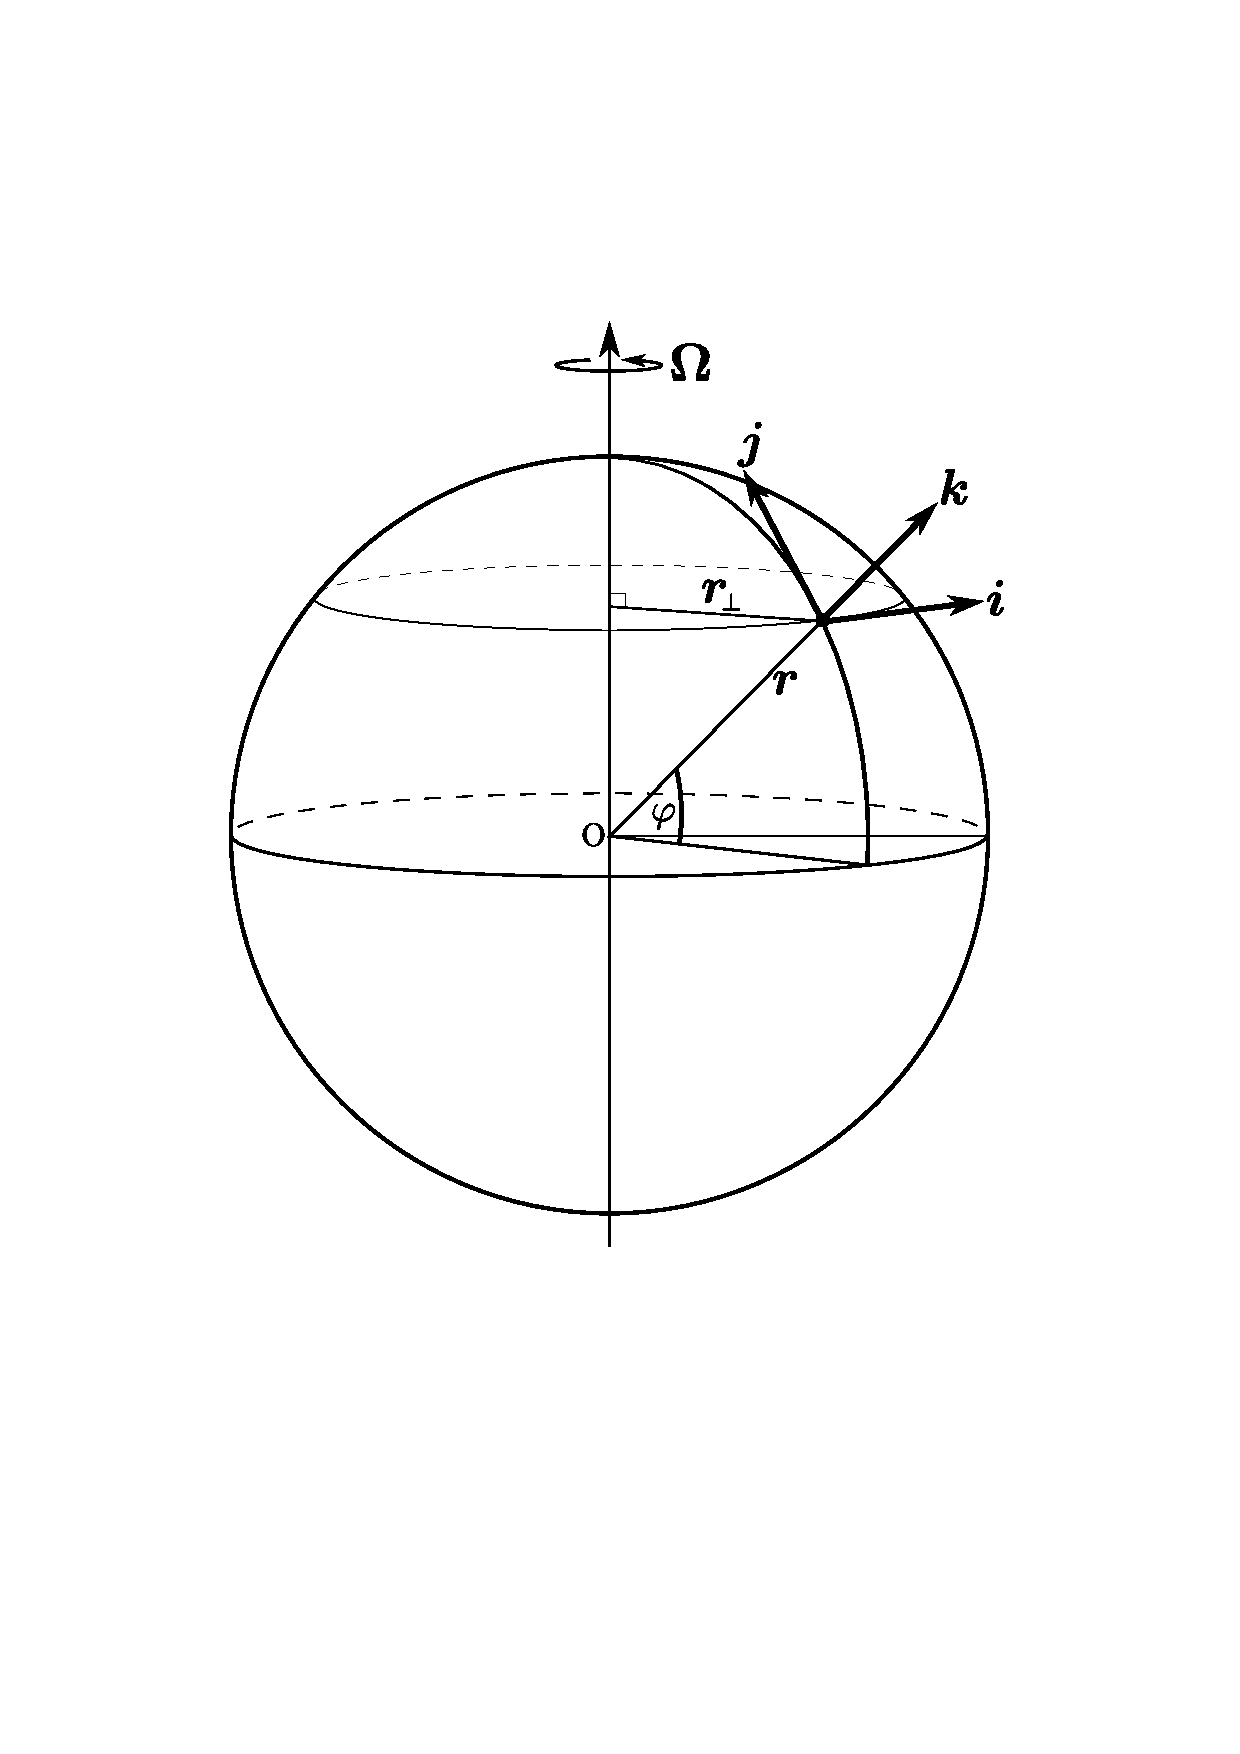
\includegraphics[width=8.0cm]{misc_images/coordinates.pdf}
\caption{Schematic of coordinates in a frame rotating with a sphere. The rotation is about a vector
pointing from South to North pole. A point on the surface of the sphere $\bmx$ and its perpendicular
distance from the axes of rotation $\bmx_{\perp}$ are shown. The latitude of $\bmx$ is given by $\phi$ 
and the unit vectors $\bmi$, $\bmj$ and $\bmk$ represent a local coordinate axes at point $\bmx$ in the rotating
frame: $\bmi$ points Eastwards, $\bmj$ points Northwards and $\bmk$ points in the radial outwards direction.}
\end{figure}

It is possible to form the equations with respect to a moving reference frame as long as the
additional force or acceleration term is included. In the case of a rotating frame that is
just by replacing the material derivative in the momentum equation by
\begin{equation}
\DDt{\bmu} + 2\bmOmega\times\bmu,
\end{equation}
where $\bmOmega$ is the angular velocity vector of the rotating
system.

Consider the Earth with a rotation vector in an inertial reference frame given by 
\begin{equation}\label{eq:on_sphere_rotation}
\bmOmega=(0,0,\Omega)^T.
\end{equation}
In a local rotating frame of reference where the
$x$-axis is oriented Eastwards,
the $y$-axis is oriented Northwards and the $z$-axis is the local upwards direction,
the Earth's rotation vector is expressed as
\begin{equation*}
\bmOmega = \Omega \cos \phi\; {\bf j} + \Omega \sin \phi\; {\bf k} \equiv \Omega (0,\cos\phi,\sin\phi)^T,
\end{equation*}
where $\phi$ is the latitude.
The acceleration terms in the three momentum equations now have the form
{\setlength\arraycolsep{2pt}
\begin{eqnarray*}
&&\DDt{u} {\color{red}+} {\color{red}2\Omega\cos\phi\; w} - 2\Omega\sin\phi\; v,\\
&&\DDt{v} + 2\Omega\sin\phi\; u,\\
&&\DDt{w} {\color{red}-} {\color{red}2\Omega\cos\phi\; v}.
\end{eqnarray*}}

\subsubsection{The `traditional' approximation}
\index{traditional approximation}
Define the Coriolis and reciprocal Coriolis parameters \citep{cushman1994} respectively by
\begin{equation}\label{eq:coriolis_parameters} 
f=2\Omega\sin\phi,\quad f^*=2\Omega\cos\phi.
\end{equation}
Due to dimensional considerations it is is usual to
drop the $f^*$ term and hence simply assume that 
\begin{equation}\label{eq:f_omega}
\bmOmega=(0,0,f/2)^T,
\end{equation}
in the local frame of reference, \ie only to consider the locally vertical
component of the rotation vector.
This approximation, when taken along with the assumption of hydrostatic balance in the
vertical constitutes what is generally known as the traditional approximation in geophysical fluid
dynamics.


\subsubsection{The $f$-plane and $\beta$-plane approximations}
\index{Coriolis!f-plane@$f$-plane}
\index{Coriolis!b-plane@$\beta$-plane}
If the Coriolis parameter $f$ is approximated by a constant value:
\begin{equation}\label{eq:f-plane}
f=f_0,
\end{equation}
this is termed the $f$-plane approximation, 
where $f_0 = 2\Omega\sin\phi_0$ at a latitude $\phi_0$.
This is obviously only an applicable approximation in a domain of interest 
that does not have large extent in latitude. 

For slightly larger domains a more accurate approximation is to use
\begin{equation}\label{eq:beta-plane}
f = f_0 + \beta y,
\end{equation}
where $y$ is the local coordinate in the Northwards direction.
Taking $\phi = \phi_0 + y/R_E$ and expanding \eqref{eq:coriolis_parameters} 
in a Taylor series yields
\begin{equation*}
f = f_0 +2\Omega\cos\phi_0\frac{y}{R_E}+\ldots,\quad \beta = \frac{2\Omega}{R_E}\cos\phi_0,
\end{equation*}
where $R_E\approx\unit[6378]{km}$. Typical values of these terms are: 
\begin{equation*}
\Omega = \frac{2\pi}{24\times 60\times 60} = 7.2722\times 10^{-5}\rads[],
\end{equation*}
(NB. a sidereal day should be used to give a more accurate value of $7.2921\times 10^{-5}\rads[]$)
and
\begin{center}\begin{small}
\begin{tabular}{c|ccc}
  &  $\phi_0 = 30$ & $\phi_0=45$ & $\phi_0 = 60$ \\  \hline
 $f_0$  & 7.2722e-05 & 1.0284e-04 & 1.2596e-04 \\
 $\beta$  & 1.9750e-11  &  1.6124e-11  &  1.1402e-11 \\
\end{tabular}\end{small}
\end{center}

\subsection{Linear Momentum}
\index{linear momentum}

Newton's second law states that the sum of forces applied to a body is equal to the time derivative of linear momentum of the body,
\begin{equation}\label{Newtons2nd}
 \sum \vec f = \d(m\vec u)/\d t.
\end{equation}
Applying this law to a control volume\footnote{The concept of a control volume and how they are defined within fluidity is discussed more in section \ref{ControlVolumeAdvection}} of fluid and making use of equation \ref{RTT} leads to the linear momentum equation for a fluid which can be written as
\begin{equation}\label{LinMom}
 \frac{\partial}{\partial t}\int_{V}\rho\vec u \d V = -\int_{S} \vec u \rho \vec u\cdot\vec n \d A+\int_{V}\vec F\rho \d V
                                                      +\int_{S} \sigtens\cdot\vec n \d A,
\end{equation}
where $V$ is the control volume, $S$ is the surface of the control volume and $\vec n$ is the unit normal to the surface of the control volume and $\vec F$ is a volume force per unit mass. Physically, \ref{LinMom} states that the sum of all forces applied on the control volume is equal to the sum of the rate of change of momentum inside the control volume and the net flux of momentum through the control surface. More details regarding the derivation and properties of this equation can be found in \citet{batchelor1967}.

\subsection{Buoyancy and Hydrostacy}\label{sect:hydrostacy}
\index{density}
\index{buoyancy}
\index{pressure!hydrostatic}

For fluids upon which gravity is acting the buoyancy force should be considered
when a free surface is present or when the fluid contains variations in density. The buoyancy force is given by $\vec{b}=-\rho\bmg$
and, in the absence of viscosity, a simple form of the vertical momentum equation can be written as
\begin{equation}\label{eq:vertmom}
\DDt[t]{w} = -\ppx[z]{p} + b,
\end{equation}
where $b=\rho g$ is the magnitude of the buoyancy force.

\index{density!reference}
\index{pressure!perturbation}

If the fluid is in a state of rest, the left hand side of \eqref{eq:vertmom} is zero giving
\begin{equation}\label{eq:hydrostatic_balance}
\ppx[z]{p} = b.
\end{equation}
This is known as hydrostatic balance. It states that the pressure at point
is equal to the weight of water above that point, plus any pressure loading on the surface of the
domain (\eg atmospheric pressure or ice load which is here termed $p_a$):
\begin{equation*}
p(\bmx) = p_a + \int_z b.
\end{equation*}
If vertical accelerations are negligible then \eqref{eq:hydrostatic_balance} is
often a good approximation to \eqref{eq:vertmom}. Under this assumption it is natural
to define pressure in terms of a background pressure that is
only dependent on depth and a perturbation to this:
\begin{equation*}
p=p_0(z,t)+p'(\bmx,t),
\end{equation*}
where $p_0(z,t)$ balances the constant $\rho_0$ part of buoyancy and may be written
\begin{equation*}
p_0(z,t) = \int_z^\eta \rho_0 g = \rho_0 g(\eta - z),
\end{equation*}
where $\eta\equiv\eta(\vec x)$ is the free surface height. If a free surface is present an
additional term of the form
\begin{equation*}
-\rho_0g\nabla\eta,
\end{equation*}
must therefore be included in the horizontal momentum equations.

\subsection{The Boussinesq approximation} \label{sect:boussinesq_approximation}
\index{density!reference}
\index{Boussinesq!approximation}

Under certain conditions, one is able to assume that density does not vary greatly about a mean reference density, that is, the density at a position $\vec x$ can be wriiten as
\begin{equation}
\rho(\bmx,t) = \rho_0 + \rho'(\bmx,t),
\end{equation}
where $\rho'\ll\rho_0$. Such an approximation, namely, the Boussinesq approximation, involves two steps. The first makes use of \eqref{eq:divfree} --- mass conservation thus becomes volume conservation and sound waves are filtered. The second part of the Boussinesq approximation follows by replacing $\rho$ by $\rho_0$ in all terms of \eqref{viscous_fluids_1}, except where density is multiplied by gravity (i.e. in the buoyancy term where full density must be retained --- these are the density variations that drive natural convection). This yields
\begin{equation}
\rho_0\DDt{\bmu} -\nabla\cdot\sigtens = \rho \bmg + \rho_0\bmF,
\end{equation}
where buoyancy has explicitly been removed from the forcing term $\bmF$ and $\bmg$ is the gravitational vector (e.g. $\bmg = -g\bmk$ in planar problems when gravity points in the negative $z$ direction and $\bmg = -g\vec r$ on the sphere).

\subsubsection{The non-hydrostatic Boussinesq equations}\label{sect:typical_ICOM_equations}
\index{Boussinesq!equations}
\index{momentum equation}
\index{continuity equation}

Applying the approximations outlined in section \ref{sect:boussinesq_approximation} to (\ref{viscous_fluids_1}) and (\ref{mass_conservation_2}), along with scalar transport equations for salinity and temperature (see (\ref{eq:general_scalar_eqn})) and an appropriate equation of state (see section \ref{sect:equation_of_state}), the three-dimensional non-hydrostatic Boussinesq equations can be written as

\begin{subeqnarray}
\frac{\pp\bmu}{\pp t} + \bmu\cdot\nabla \bmu + 2 \bmOmega \times \bmu
&=& - \nabla p' - g\nabla\eta + \rho' \bmg + \nabla\cdot \tautens + \bmF,
\slabel{mtm}\\
\nabla\cdot {\bmu}&=&0,\slabel{conty}\\
\frac{\pp T}{\pp t} + \bmu\cdot\nabla  T  &=&
\nabla . \left ( \kaptens_T  \nabla T\right),\slabel{heat}\\
\frac{\pp S}{\pp t} + \bmu\cdot\nabla  S  &=&
\nabla . \left ( \kaptens_S  \nabla S\right),\slabel{salt}\\
f(p,\rho,T,\ldots)&=&0,\slabel{state}
\label{boussinesq}
\end{subeqnarray}

where $p'$ is the perturbation pressure (see section \ref{sect:hydrostacy}),
$\rho=\rho_0+\rho'$ where $\rho'(=(\rho-\rho_0)/\rho_0)$ is the perturbation density,
$T$ is the temperature, $S$ is salinity, $\eta$ is the free surface height and
$\tautens,\kaptens_T,\kaptens_S$ are the viscosity, thermal diffusivity and saline
diffusivity tensors respectively.
The rotation vector is $\bmOmega$, and $\bmF$ contains additional source terms such as the astronomical tidal forcing. A discussion
regarding the validity of the Boussinesq approximation is given in \cite{Gray1976}

\subsection{Supplementary boundary conditions and body forces}

\subsubsection{Bulk parameterisations for oceans}
\index{boundary conditions!bulk parameterisations}

In order to simulate real-world ocean scenarios, realistic boundary conditions for the momentum, freshwater and heat fluxes 
must be applied to the upper ocean surface. \fluidity can apply such boundary conditions in the form of the bulk formulae of \citet{large2004},
COARE 3.0 \citep{fairall2003} and \citet{kara2005} in combination with the ERA-40 reanalysis data \citep{Uppala2005}.

Three surface kinematic fluxes calculated: heat -- $\langle w\theta \rangle$,
salt -- $\langle ws \rangle$, and momentum -- $\langle wu \rangle$ and $\langle wv \rangle$,
which can be related to the surface fluxes of heat $Q$, the
freshwater $F$, and the momentum $\overrightarrow\tau=\left(\tau_u,\tau_v\right)$, via:
\begin{align}
\langle w\theta \rangle &= Q\left(\rho C_p \right)^{-1} \\
\langle ws \rangle &= F\left(\rho^{-1}S_0\right) \\
\left(\langle wu \rangle, \langle wv \rangle\right) &=
\overrightarrow{\tau}\rho^{-1} =
\left(\tau_u,\tau_v\right)\rho^{-1}
\end{align}
where $\rho$ is the ocean density, $C_p$ is the heat capacity (4000 Jk$S^{-1}$K$^{-1}$) 
and $S_0$ is a reference ocean salinity, which is the current sea surface salinity. 
These fluxes are then applied as upper-surface Neumann boundary conditions on
the appropriate fields.

\subsubsection{Co-oscillating boundary tides}
\index{boundary conditions!boundary tides}
\label{sec:boundary_tide}

Boundary tides can be applied to open ocean domain boundaries through setting a Dirichlet condition on the non-hydrostatic part of the pressure. Co-oscillating tides are forced as cosine waves of specified phase and amplitude along designated boundaries:
\begin{equation}
h=\sum_{i}A_{i}\cos(\sigma_{i} t -\phi_{i})
+\sum_{j}A_{j}\cos(\sigma_{j} t -\phi_{j})
+\sum_{k}A_{k}\cos(\sigma_{k} t -\phi_{k}),
\label{eq:co-oscillating-tide}
\end{equation}
where $h$ is the free surface height (m), $A$ is the amplitude of the tidal 
constituent (m), $t$ is the time (s), $\phi$ is the phase of the tidal constituent 
(radians) \citep{Wells2008}. 
 
The nature of the co-oscillating tide can take the form of either one fixed cosine wave of constant amplitude 
and phase applied across the entire length of the boundary, or it can be variable as delimited via an 
interpolation of different amplitudes and phases at a series of points spread along the boundary \citep{Wells2008}.
Within \fluidity, co-oscillating boundary tides can be applied through \eg the FES2004 data set (see \ref{sect:tides_in_the_med}).

\subsubsection{Astronomical tides}\label{Sect:AST}
\index{body forces!astronomical tides}
\label{astronomical}

Astronomical forcing can also be applied to a fluid as a body force\footnote{Note that use of the word body force in this context should not be confused with the application of a body force through the options tree discussed later in \ref{chap:configuration}. The astronomical forcing is applied separately.}. 
The astronomical tidal potential is calculated at each node of the finite element mesh using the 
multi-constituent equilibrium theory of tides equation:
  \begin{eqnarray}
\eta_{eq}\left(\lambda,\theta,t\right)&=&\sin^{2}\theta\sum_{i}A_{i}\cos\left(\sigma_{i}t+\chi_{i}+2\lambda\right)\nonumber\\
&+&\sin2\theta\sum_{j}A_{j}\cos\left(\sigma_{j}t+\chi_{j}+\lambda\right)\\
&+&\left(3\sin^{2}\theta-2\right)\sum_{k}A_{k}\cos\left(\sigma_{k}t+\chi_{k}\right)\nonumber,
\label{eq:multi-constituent-eq_theory}
  \end{eqnarray}
where $\eta_{eq}$ is the equilibrium tidal potential (m), $\lambda$ is the east longitude (radians), $\theta$ is the colatitude
$[(\pi/2)-{\text{latitude}}]$, $\chi$ is the astronomical argument (radians), $\sigma$
is the frequency of the tidal constituent (s$^{\text{-1}}$), $t$ is universal standard
time (s) and $A$ is the equilibrium amplitude of the tidal constituent (m). Subscript
$i$ represents the semidiurnal constituents (e.g. M$_{\text{2}}$), subscript $j$
the diurnal constituents (\eg K$_{\text{1}}$) and subscript $k$ the long period
constituents (\eg M$_{\text{f}}$; \citealp{Wells2008}).   
The overall forcing 
is applied as the product of the gradient of the resulting equilibrium tidal potential and the acceleration due 
to gravity (g) \citep{Mellor1996, Kantha2000, Wells2007}.
The multi-constituent equilibrium theory of tides is flexible in that it enables astronomical tides to be forced as 
individual constituents 
(e.g. M$_{2}$ or S$_{2}$) or as a combination of different constituents (e.g. M$_{2}$ + S$_{2}$) \citep{Wells2008}.

As there is no interest in calculating the tide for an exact date, the astronomical argument 
is typically excluded from the multi-constituent theory of tides equation for ICOM applications meaning that all satellites 
start at 0$^{\circ}$ latitude \citep{Wells2008}.

The astronomical tidal potential can be modified to account for the deformation of the solid earth
(the body tide) if desired. The multi-constituent equilibrium theory of tides equation includes the effects of the
solid earth deformation, adding this to the overall free surface height. 
This is fine
when validating model results against measurements that record the overall elevation of the 
Earth's oceans (e.g. satellite altimeter readings and surface tide gauges). If however, the model
is validated against measurements that do not include the effects of the Earth's body tide
such as with pelagic pressure gauges, then a correction to the equilibrium tidal potential
is required. This can be applied as: 
\begin{equation}
\eta=(1+k-h)\eta_{eq},
\label{eq:body-tide}
\end{equation}    
where $\eta$ is the corrected tidal potential, $\eta_{eq}$ is the uncorrected equilibrium tidal potential
and $k$ (0.3) and $h$ (0.61) are Love numbers (after \citealp{Love1909}).
Both $k$ and $h$ are dimensionless measures of the elastic behavior of the solid Earth. $k$ accounts for the enhancement to the
Earth's gravitational potential brought about by the re-distribution of the Earth's mass whereas $h$
is a correction for the physical distortion to the Earth's surface \citep{Pugh1987}.

The exact values of $k$ and $h$ vary for different tidal constituents and the numbers shown are given
for the semidiurnal M$_{\text{2}}$ constituent. Typical variations to $k$ and $h$ are less than 0.01 which
corresponds to a $<$1\% change to the equilibrium tidal potential.
These errors are sufficiently small that the stated values are a suitable approximation to
use in body tide corrections to the majority of tidal constituents.

\subsection{Multi-material simulations}
\index{multi-material flow}
The ability to differentiate between regions with distinct material properties is of fundamental importance in the modeling of many physical systems. Two different approaches exist for achieving this: the multi-material approach and the multi-phase approach. The multi-material approach is implemented within \fluidity, and the multi-phase approach (discussed in the next subsection) is currently under development.
In situations where the model can resolve physical mixing of immiscible materials, or where there is no mixing, only one velocity field (and hence one momentum equation) is required to describe the flow of all materials. The \emph{multi-material} approach, considers all materials to be immiscible materials separated by a sharp interface.

In a multi-material approach, the various forms of the conservation equations can be solved for multiple material flows if the point-wise mass density $\rho$ in the equations is defined as the bulk density at each point.  If the flow comprises $n$ materials and the volume fraction of the $i^{th}$ material is denoted $\phi_i$ then the bulk density is given by:
\begin{equation}
\rho = \sum_{i=1}^n \phi_i\rho_i
\end{equation}
where $\rho_i$ is the density of each material.  For incompressible materials $\rho_i = \rho_{i0}$; for materials whose density is defined by an equation of state (see section~\ref{sect:equation_of_state}) $\rho_i = f(p,T,S,\ldots)$.  Conservation of mass at each point also requires that
\begin{equation}
\sum_{i=1}^n \phi_{i} = 1.
\end{equation}

In an $n$-material problem, the multi-material approach requires that $n-1$ advection equations are solved, to describe the transport of the volume fraction of all but one of the materials.  The volume fraction of the remaining material can be derived from the other volume fractions by
\begin{equation}\label{diagnosticvolfrac}
\phi_{n} = 1 - \sum_{i=1}^{n-1}\phi_{i}. 
\end{equation}
The transport of the $i^{th}$ volume fraction is given by  
\begin{equation}
\ppt{\phi_i} + \bmu\cdot\nabla\phi_i = 0,
\end{equation}
where the volume fraction field at time zero must be specified.

\subsection{Multi-phase simulations}
\index{multi-phase flow}
Multi-phase flows are defined by \cite{prosperettiEtAl2007} to be flows in which two or more phases of matter (solid, liquid, gas, etc) are simultaneously present and are allowed to inter-penetrate. Simple examples include the flow of a fizzy drink which is composed of a liquid and a finite number of gas bubbles, the transportation of solid sediment particles in a river, and the flow of blood cells around the human body.

Further to the above definition, each phase is classed as either \textit{continuous} or \textit{dispersed}, where a continuous phase is a connected liquid or gas substance in which dispersed phases (comprising a finite number of solid particles, liquid droplets and/or gas bubbles) may be immersed \citep{croweEtAl1998}.

To enable the mixing and inter-penetration of phases, a separate velocity field (and hence a separate set of continuity and momentum equations) is assigned to each one and solved for. Extra terms are then included to account for inter-phase interactions. Thus, for each phase $i$, the governing equations (based on those derived in \cite{ishii1975}) are:
\begin{equation}
\frac{\partial}{\partial t}\left(\alpha_i\rho_i\right) + \nabla\cdot\left(\alpha_i\rho_i\mathbf{u}_i\right) = 0,
\end{equation}
\begin{equation}
\frac{\partial}{\partial t}\left(\alpha_i\rho_i\mathbf{u}_i\right) +
\nabla\cdot\left(\alpha_i\rho_i\mathbf{u}_i\mathbf{u}_i\right) =
-\alpha_i\nabla p + \alpha_i\rho_i\mathbf{g} +
\nabla\cdot\left(\alpha_i\tautens_i\right) +
\mathbf{F}_i,
\end{equation}
where $\mathbf{u}_i$, $\rho_i$, $\tautens_i$ and $\alpha_i$ are the velocity, density, stress tensor and volume fraction of phase $i$ respectively, and $\mathbf{F}_i$ represents the forces imposed on phase $i$ by the other $N-1$ phases. The model currently assumes a common pressure field $p$ and no mass transfer between phases. Details of momentum transfer terms are given in Chapter \ref{chap:configuration}.

\chapter{Numerical discretisation}\label{chap:numerical_discretisation}
\section{Introduction \& some definitions}\label{Sect:ND_Intro}
This chapter covers the numerical discretisation of the model equations
given in the previous chapter as they are assembled and solved 
in \fluidity. For a more general introduction into finite element theory
we refer to a.o. \cite{elman2005} and \cite{gresho1988}.

In this chapter we define the domain we are solving over as $\Omega$. The boundary to
$\Omega$ is defined as $\dOmega$
%(NB. $\Gamma$ is another common symbol for a boundary) 
and can be split into different sections, e.g.
$\partial\Omega = \dOmega^{N}\cup \dOmega^{D}$
where $\dOmega^{N}$ is that part of the boundary over
which Neumann conditions are applied and $\dOmega^{D}$ is that part of the boundary over
which Dirichlet conditions are applied. For clarity a subscript showing the field in question will
be given on the $N$ and $D$ characters.

The unit vector \vec{n} is always assumed to be the
outward facing normal vector to the domain.
In the following this notation is used to describe both the normal vector at the boundary
and between elements in the interior.

\section{Spatial discretisation of the advection-diffusion equation}
\label{Sect:ND_advection_diffusion_discretisation}

The advection-diffusion equation for a scalar tracer $c$,
is given in conservative form by
\begin{equation}\label{eq:advdif}
  \ppt{c} + \div\left(\vec{u} c\right) - \div\tensor{\kappa}\cdot\grad c = 0.
\end{equation}

We now define a partition of the boundary such that
$\partial\Omega = \dOmega^{N}\cup \dOmega^{D}$, and impose boundary conditions on $c$:
\begin{gather}
  \label{eq:cboundary}
  \vec{n}\cdot\tensor{\kappa}\cdot\grad c=g_{N_c} \quad\textrm{on}\quad \dOmega^{N_c},\\
  c=g_{D_c} \quad\textrm{on}\quad \dOmega^{D_c}.
\end{gather}

\subsection{Continuous Galerkin discretisation}
\label{sect:ND_advection_diffusion_CG}

The Continuous Galerkin method (often abbreviated to CG, 
not to be confused with Conjugate Gradients) method,
is a widely used finite element method in which 
the solution fields are constrained to be
continuous between elements. 
The fields are only assumed to be $C^0$
continuous, that is to say there is no assumption that the gradient of a
field is continuous over element boundaries.

\subsubsection{Weak form}
\index{weak form}
\index{test function}
\index{advection-diffusion equation!weak form}

Development of the finite element method begins by writing the equations in
\emph{weak form}.  The weak form of the advection-diffusion equation 
(here presented in conservative form) is
obtained by pre-multiplying it with a test function $\phi$
and integrating over the domain $\Omega$, such that
\begin{equation}
  \int_\Omega \phi \left( \ppt{c} + \grad\cdot(\vec{u} c) -
    \div\tensor{\kappa}\cdot \grad c\right) = 0.
\end{equation}
Integrating the advection and diffusion terms by parts yields
\begin{equation}\label{eq:weak_adv_diff}
  \int_\Omega
  \phi \ppt{c}
  -\grad\phi\cdot\vec{u} c +
  \grad\phi\cdot \tensor{\kappa}\cdot\grad c
  +\int_\dOmega \phi(\vec{n}\cdot \vec{u} c
  - \vec{n}\cdot\tensor{\kappa}\cdot\grad c)
  = 0.
\end{equation}
For simplicity sake let us first assume the boundaries are closed
($\vec{u}\cdot\vec{n}=0$) and we apply a homogeneous Neumann boundary
condition everywhere, such that $\partial c/\partial n=0$, which gives
\begin{equation}\label{eq:weak_adv_diff_simp}
  \int_\Omega \phi \frac{\partial c}{\partial t}
    -\grad\phi\cdot\vec{u} c +
    \grad\phi\cdot \tensor{\kappa}\cdot\grad c = 0.
\end{equation}
Note that due to the Neumann boundary condition the boundary term has
dropped out. The tracer field $c$ is now called a \emph{weak solution} of
the equations if \eqref{eq:weak_adv_diff_simp} holds true for all $\phi$ in some
space of test functions $V$. The choice of a suitable test space $V$ is dependent
on the equation (for more details see \citet{elman2005}).

\index{Sobolev space} An important observation is that
\eqref{eq:weak_adv_diff} only contains first derivatives of the field $c$,
so that we can now include solutions that do not have a continuous second
derivative. For these solutions the original equation \eqref{heat} would not
be well-defined. These solutions are termed \emph{weak} as they do not
have sufficient smoothness to be \emph{classical} solutions to the problem.
All that is required for the weak solution is that the first derivatives of $c$
can be integrated along with the test function. A more precise definition of
this space, the \emph{Sobolev space}, can again be found \citet{elman2005}.

\subsubsection{Finite element discretisation}
\index{trial function}
Instead of looking for a solution in the entire function (Sobolev) space,
in finite element methods discretisation is performed by restricting the solution to a
finite-dimensional subspace. Thus the solution can be
written as a linear combination of a finite number of functions,
the \emph{trial functions} $\phi_i$ that form a basis of the
\emph{trial space}, defined such that
\begin{equation*}
  c(\vec{x})=\sum_i c_i \phi_i(\vec(x)).
\end{equation*}
The coefficients $c_i$ can be written in vector format. The
dimension of this vector equals the dimension of the trial
space. In the sequel any function in
this way represented as a vector will be denoted as $\dvec{c}$.

\index{Galerkin!methods}
\index{Galerkin!projection}
Since the set of trial functions is now much smaller (or rather finite as opposed to infinite-dimensional), we also need
a much reduced set of test functions for the equation in weak
form \eqref{eq:weak_adv_diff_simp} in order to find a unique
solution. A common choice is, in fact, to choose the same
test and trial space. Finite element methods that make this choice are
referred to as \emph{Galerkin methods} --- the discretisation
can be seen as a so called \emph{Galerkin
projection} of the weak equation to a finite subspace.

\index{PN@\PN}
\index{Galerkin!continuous}
\index{Galerkin!discontinuous}
There are many possibilities for choosing the finite-dimensional trial and test spaces.
A straightforward choice is to restrict the functions to be polynomials of degree
$n\leq N$ within each element. These are referred to as \PN discretisations.
As we generally need functions for which the first
derivatives are integrable, a further restriction
is needed. If we allow the functions to be any polynomial of
degree $n\leq N$ within the elements the function can be
discontinuous in the boundary between elements.
Continuous Galerkin methods therefore
restrict the test and trial functions to arbitrary polynomials
that are continuous between the elements. Discontinuous Galerkin methods,
that allow any polynomial, are also possible but require
extra care when integrating by parts (see section \ref{sec:NM_DG_advection}).

\index{P1@\Pone}
\index{basis function}
If we choose \Pone as our test and trial functions, \ie piecewise linear
functions, within each element we only need to know the value
of the function at 3 points in 2D, and 4 points in 3D.
In \fluidity\ these points are chosen to be the vertices of
the triangles (in 2D) or tetrahedra (in 3D) tessellating the domain.
For continuous Galerkin the continuity
requirement then comes down to requiring
the functions to have a single value at each
vertex. A set of basis functions $\phi_i$
for this space is easily found by choosing the piecewise linear functions
$\phi_i$ that satisfy:
\begin{gather*}
  \phi_i(x_i)=1, \;\forall i\\
  \phi_i(x_{j\neq i})=0,\;\forall i,j,
\end{gather*}
where $x_i$ are the vertices in the mesh.
This choice of basis functions has the following useful property:
\begin{equation*}
  c_i=c(\vec{x}_i),\quad \text{for all nodes $x_i$ in the mesh.}
\end{equation*}
This naturally describes trial functions that are linearly
interpolated between the values $c_i$ in the nodes.
Higher order polynomials can be represented using more
nodes in the element (see Figure \ref{fig:cgshapefunctions}).

\begin{figure}[btp]
\begin{center}
\begin{tabular}{lr}
\xfig{numerical_discretisation_images/P1cgshapefunction1d} & \xfig{numerical_discretisation_images/P2cgshapefunction1d} \\
\xfig{numerical_discretisation_images/P1cgshapefunction2d} & \xfig{numerical_discretisation_images/P2cgshapefunction2d}
\end{tabular}
\caption{One-dimensional (a, b) and two-dimensional (c, d) schematics of piecewise linear (a, c) and piecewise quadratic (b, d) continuous shape functions.  The shape function has value $1$ at node $A$ descending to $0$ at all surrounding nodes.  The number of nodes per element, $e$, depends on the polynomial order while the support, $s$, extends to all the elements surrounding node $A$.}
\label{fig:cgshapefunctions}
\end{center}
\end{figure}

As discussed previously the test space in Galerkin finite element methods is the same as the
trial space. So for \PN the test functions can be an arbitrary linear combination
of the same set of basis functions. To make sure that the equation we are solving
integrates to zero with all such test functions, all we have to do is make sure
that the equation tested with the basis functions integrate to zero. The discretised
version of \eqref{eq:weak_adv_diff_simp} therefore becomes
\index{advection-diffusion equation!weak form!discretised}
\begin{equation}
  \sum_j \left\{ \int_\Omega \phi_i \phi_j  \ddt{c_j} -
    \grad\phi_i\cdot\vec{u}\phi_j  c_j +
    \grad\phi_i\cdot \tensor{\kappa}\cdot\grad \phi_j c_j \right\} = 0,
    \quad\text{for all }\phi_i.
\end{equation}
where we have substituted $c=\sum_j \phi_j c_j$. From this it is readily seen that
we have in fact obtained a matrix equation of the following form
\begin{equation}
  \mat{M} \ddt{\dvec{c}}+\mat{A}(\vec{u})\dvec{c}+\mat{K}\dvec{c}=0,
  \label{eq:cg_adv_diff_mat}
\end{equation}
where $\mat{M}, \mat{A}$ and $\mat{K}$ are the following matrices
\begin{equation}
  \mat{M}_{ij}=\int_\Omega \phi_i\phi_j, \quad
  \mat{A}_{ij}=-\int_\Omega \grad\phi_i\cdot\vec{u} \phi_j, \quad
  \mat{K}_{ij}=\int_\Omega \grad\phi_i\cdot \tensor{\kappa}\cdot\grad \phi_j.
\end{equation}

\subsubsection{Advective stabilisation for CG}
\label{Sect:ND_advective_stabilisation_CG}
\index{advection-diffusion equation!continuous Galerkin}
\index{Galerkin!continuous!advection}
\index{stabilisation!advection}

It is well known that a continuous Galerkin discretisation of an
advection-diffusion equation for an advection dominated flow can suffer from
over- and under-shoots which are qualitatively incorrect errors. Furthermore, these overshoot errors are not
localised: they can propagate throughout the simulation domain and pollute the
global solution \citep{hughes1987}. Consider a simple 1D linear steady-state
advection-diffusion problem for a single scalar $c$ with a source term $f$:

\begin{equation}\label{eqn:trivial_advdif}
  u \ppx{c} - \kappa \ppxx{c} = f(x),
\end{equation}
or equivalently in weak form:
\begin{equation}\label{eqn:trivial_advdif_weak}
  \int_\Omega \left\{\phi \left( u \ppx{c} -f \right) + \kappa \ppx{\phi} \ppx{c}\right\}  = 0,
\end{equation}
where we have integrated by parts and applied the natural Neumann boundary
condition $\partial c / \partial x = 0$ on $\partial \Omega$.
Discretising \eqref{eqn:trivial_advdif_weak} with a continuous Galerkin method
leads to truncation errors in the advection term equivalent to a negative
diffusivity term of magnitude \citep{DoneaBook}:
\begin{equation}\label{eqn:cg_implicit_diffusivity}
  \bar{\kappa} = \xi \kappa \Pe,
\end{equation}
where:
\begin{equation}\label{eqn:xi_parameter}
  \xi = \frac{1}{\tanh(\Pe)} - \frac{1}{\Pe},
\end{equation}
and:
\begin{equation}\label{eqn:grid_pe}
  \Pe = \frac{u h}{2 \kappa},
\end{equation}
is a grid P\'eclet number, with grid spacing $h$.
\index{P\'eclet number!grid}

This implicit negative diffusivity becomes
equal to the explicit diffusivity at a P\'eclet greater than one, and hence
instability can occur for $\Pe \geq 1$. In order to achieve a stable discretisation
using a continuous Galerkin method one is therefore required either to increase
the model resolution so as to reduce the grid P\'eclet number, or to apply
advective stabilisation methods.

\paragraph{Balancing diffusion}\label{sec:balancing_diffusion}
\index{stabilisation!advection!balancing diffusion}

A simple way to stabilise the system is to add an extra diffusivity of
equal magnitude to that introduced by the discretisation of the advection term,
but of opposite sign. This method is referred to as \textit{balancing diffusion}.
Note, however, that for two or more dimensions, we require this balancing
diffusion to apply in the along-stream direction only \citep{brooks1982, DoneaBook}.
For this reason this method is also referred to as \textit{streamline-upwind}
stabilisation. The multi-dimensional weak-form (assuming we consider non-conservative or advective form) 
of equation \eqref{eqn:trivial_advdif} is:
\begin{equation}\label{eqn:trivial_advdif_weak_md}
  \int_\Omega \left\{ \phi \left(\vec{u} \cdot \grad c -f \right)+ \grad \phi \cdot \tensor{\kappa}  \cdot \grad c -f)\right\} = 0,
\end{equation}
is therefore modified to include an additional artificial balancing diffusion
term \citep{DoneaBook}:
\begin{equation}\label{eqn:balancing_diffusion}
  \int_\Omega \phi (\vec{u} \cdot \grad c + \tensor{\kappa} \grad \phi \cdot \grad c - f(x)) +
  \int_\Omega \frac{\tensor{\kappa}}{\left|\left| \vec{u} \right|\right|^2}
  (\vec{u} \cdot \grad \phi) (\vec{u} \cdot \grad \vec{c})
  = 0.
\end{equation}

The exact form of the multidimensional stability parameter $\bar{\kappa}$
is a research issue. See \ref{sec:stabilisation_parameter} for implementations in
\fluidity.

The addition of the balancing diffusion term combats the negative implicit
diffusivity of the continuous Galerkin method. However, we are no longer solving
the original equation -- for pure advection we are now solving a modified
version of the original equation with the grid
P\'eclet number artificially reduced from
infinity to unity everywhere. Hence streamline-upwind is not a \textit{consistent}
stabilisation method, and there can be a reduction in the degree of numerical
convergence.

\paragraph{Streamline-upwind Petrov-Galerkin (SUPG)}\label{sec:supg}
\index{Galerkin!Petrov-}
\index{Petrov-Galerkin}
\index{stabilisation!advection!Petrov-Galerkin}

The streamline-upwind stabilisation method can be extended to a consistent (and
hence high order accurate) method by introducing stabilisation in the form of a weighted
residual \citep{DoneaBook}:
\begin{equation*}
  \int_\Omega \phi (\vec{u} \cdot \grad c + \tensor\kappa \grad \phi \cdot \grad c - f(x)) +
  \int_\Omega \tau P(\phi) R(\phi)
  = 0,
\end{equation*}
where:
\begin{equation*}
  R(\phi) = \vec{u} \cdot \grad c - \grad\cdot\tensor{\kappa}\grad  c - f(x),
\end{equation*}
is the equation residual, $\tau$ is a stabilisation parameter and $P(\phi)$ is
some operator.
Note that this is equivalent to replacing the test function in the original
equation with $\tilde{\phi} = \phi + \tau P(\phi)$.
Looking at equation \eqref{eqn:balancing_diffusion}, it can seen that the
balancing diffusion term is equivalent to replacing the test function for the
advection term only with:
\begin{equation}\label{eqn:supg_test_function}
  \tilde{\phi} = \phi + \frac{{\kappa}}{\left|\left| \vec{u} \right|\right|^2} \vec{u} \cdot \grad.
\end{equation}

This suggests a stabilisation method whereby the test function in the advection-diffusion
equation is replaced with the test function in \eqref{eqn:supg_test_function}.
This approach defines the \textit{streamline-upwind Petrov-Galerkin} (SUPG) method. The
weighted residual formulation of this method guarantees consistency, and hence
preserves the accuracy of the method. Furthermore, while this method can
still possess under- and over-shoot errors in the presence of sharp solution
gradients, these errors remain localised \citep{hughes1987}.

\paragraph{Stabilisation parameter}\label{sec:stabilisation_parameter}

Note that, as mentioned in \ref{sec:balancing_diffusion}, the choice of
stabilisation parameter $\bar{\kappa}$ is somewhat arbitrary. \fluidity\ implements \citep{brooks1982, DoneaBook}:

\begin{equation}\label{eqn:md_nu_bar}
  \bar{\kappa} = \frac{1}{2} \sum{\xi_i u_i h_i},
\end{equation}

where $\xi$ is defined in \eqref{eqn:xi_parameter} and the summation is over the quadrature points of an individual element. The
grid spacings $h_i$ are approximated from the elemental Jacobian.

As an alternative, \citet{raymond1976} show that for
1D transient pure-advection a choice of:

\begin{equation}\label{eqn:md_nu_bar_transient}
  \bar{\kappa} = \frac{1}{\sqrt{15}} \sum{\xi_i u_i h_i},
\end{equation}

minimises phase errors.

Computing the $\xi$ factor at quadrature points is potentially expensive due to
the evaluation of a hyperbolic-tangent \eqref{eqn:xi_parameter}. Sub-optimal but more computationally
efficient approximations for $\xi$ are the \emph{critical rule} approximation \citep{brooks1982}:

\begin{equation}
  \xi = \begin{cases}
          -1 - 1 / \Pe  & \Pe < -1 \\
          0             & -1 \le \Pe \le 1 \\
          1 + 1 / \Pe   & \Pe > 1,
        \end{cases}
\end{equation}

and the \emph{doubly-asymptotic} approximation \citep{DoneaBook}:

\begin{equation}
  \xi = \begin{cases}
          \Pe / 3  & \left| \Pe \right| \le 3 \\
          \sgn(\Pe)  & \textrm{otherwise}.
        \end{cases}
\end{equation}

\paragraph{Implementation limitations}

The SUPG implementation in \fluidity\ does not modify the test function derivatives
or the face test functions. Hence the SUPG implementation is only consistent
for degree one elements with no non-zero Neumann or weak Dirichlet boundary
conditions.

SUPG is considered ready for production use for scalar advection-diffusion
equation discretisation, but is still experimental for momentum discretisation.

\subsubsection{Example}

The following example considers pure advection of a 1D top hat of unit magnitude
and width 0.25 in a periodic domain of unit size. The top hat is advected with a
Courant number of $1 / 8$. Figure \ref{fig:top_hat_cg} shows the solution after
80 timesteps using a continuous Galerkin discretisation. Figure \ref{fig:top_hat_su}
shows the solution when streamline-upwind stabilisation is applied.
Figure \ref{fig:top_hat_supg} shows the solution when streamline-upwind
Petrov-Galerkin is applied, using a stabilisation parameter as in \eqref{eqn:md_nu_bar}.

\begin{figure}[ht]
  \centering
  \fig[width=0.5\textwidth]{numerical_discretisation_images/advective_stabilisation/cg}
  \caption{Pure advection of a 1D top hat function in a periodic domain at CFL number $1 / 8$ after 80 timesteps
           using a continuous Galerkin discretisation.}
  \label{fig:top_hat_cg}
\end{figure}

\begin{figure}[ht]
  \centering
  \fig[width=0.5\textwidth]{numerical_discretisation_images/advective_stabilisation/su}
  \caption{Pure advection of a 1D top hat function in a periodic domain at CFL number $1 / 8$ after 80 timesteps
           using a continuous Galerkin discretisation with streamline-upwind
           stabilisation.}
  \label{fig:top_hat_su}
\end{figure}

\begin{figure}[ht]
  \centering
  \fig[width=0.5\textwidth]{numerical_discretisation_images/advective_stabilisation/supg}
  \caption{Pure advection of a 1D top hat function in a periodic domain at CFL number $1 / 8$ after 80 timesteps
           using a continuous Galerkin discretisation with streamline-upwind
           Petrov-Galerkin stabilisation.}
  \label{fig:top_hat_supg}
\end{figure}

\subsection{Boundary conditions}
\index{boundary conditions!Neumann!weakly imposed}
In the derivation of \eqref{eq:weak_adv_diff} we have assumed a homogeneous Neumann
boundary condition on all boundaries. If we are considering all possible
solutions $c$, the boundary term we have left out is
\begin{equation}\label{eq:missing_boundary_term}
  \int_{\partial\Omega} \phi~\vec{n}\cdot\tensor{\kappa}\cdot\grad c.
\end{equation}
A natural way of imposing an inhomogeneous Neumann boundary condition
\begin{equation*}
  \vec{n}\cdot\tensor{\kappa}\cdot\grad c=g_N,
\end{equation*}
where $g_N$ can be any prescribed function on the boundary $\partial\Omega$, is to impose it
weakly. This is done in the same way as the weak form of the advection-diffusion equation was formed:
\begin{equation}\label{eq:weak_neumann}
  \int_{\partial\Omega} \phi~\vec{n}\cdot\tensor{\kappa}\cdot\grad c=
    \int_{\partial\Omega} \phi~g_N, \quad \text{for all }\phi.
\end{equation}
Thus \eqref{eq:weak_neumann} can be used to replace the missing
boundary term \eqref{eq:missing_boundary_term} with an integral of $\phi~g_N$
over the boundary.

\index{boundary conditions!Dirichlet!weakly imposed}
In a similar way, a weakly imposed Dirichlet boundary condition can be related to an
integration by parts of the advection term. Let us consider a pure advection problem
($\tensor{\kappa}\equiv 0$). The weak form of this equation integrated by parts reads:
\begin{equation*}
  \int_\Omega \phi \frac{\partial c}{\partial t} -
    \left(\grad\cdot \phi~\vec{u}\right)~c +
    \int_{\partial\Omega} \phi \vec{n}\cdot\vec{u}~c
    = 0.
\end{equation*}
The final (boundary) term can again be substituted with a weakly imposed
boundary condition $c=g_D$.  In this case however, for physical and consequently numerical reasons, we only want to impose
this on the inflow boundary, and the original term remains for the outflow
boundary:
\begin{equation}\label{eq:adv_integrated_by_parts}
  \int_\Omega \phi \frac{\partial c}{\partial t} -
    \left(\grad\cdot \phi~\vec{u}\right)~c +
    \int_{\partial\Omega_-} \phi\vec{n}\cdot\vec{u}~g_D +
    \int_{\partial\Omega_+} \phi\vec{n}\cdot\vec{u}~c
    = 0,
\end{equation}
where $\partial\Omega_-$ and $\partial\Omega_+$ refer to respectively
the inflow ($\vec{n}\cdot\vec{u}>0$) and outflow boundaries ($\vec{n}\cdot\vec{u}<0$).

It is to be noted that when we are applying boundary conditions weakly we
still consider the full set of test functions, even those that don't satisfy
the boundary condition. This means the discrete solution will not satisfy
the boundary condition exactly. Instead the solution will converge to the
correct boundary condition along with the solution in the interior as the mesh
is refined.

\index{boundary conditions!Dirichlet!strongly imposed} An alternative way of
implementing boundary conditions, so called \emph{strongly imposed} boundary
conditions, is to restrict the trial space to only those functions that
satisfy the boundary condition. In the discrete trial space this means we no
longer allow the coefficients $c_i$ that are associated with the nodes $x_i$
on the boundary, to vary but instead substitute the imposed Dirichlet
boundary condition. As this decreases the dimension of the trial space, we
also need to limit the size of the test space. This is simply done by
removing the test function $\phi_i$ associated with the nodes $x_i$ on the
boundary, from the test space. Although this guarantees that the Dirichlet
boundary condition will be satisfied exactly, it does not at all mean that
the discrete solution converges to the exact continuous solution more
quickly than it would with weakly imposed boundary conditions. Strongly
imposed boundary conditions may sometimes be necessary if the boundary
condition needs to be imposed strictly for physical reasons.

\subsection{Discontinuous Galerkin discretisation}\label{sec:NM_DG_advection}
\index{Galerkin!discontinuous!advection}
\index{advection-diffusion equation!discontinuous Galerkin}

Integration by parts can be used to avoid taking
derivatives of discontinuous functions.
When using discontinuous test \emph{and} trial functions (see Figure \ref{fig:dgshapefunctions}) however,
neither the original advection equation, \eqref{eq:weak_adv_diff} with $\tensor{\kappa}\equiv 0$,
nor the version \eqref{eq:adv_integrated_by_parts} integrated by parts are well-defined.
Within an element $e$ however the functions are continuous, and everything is well defined. So within
a single element we may write
\begin{equation}\label{eq:adv_diff_dg}
  \int_e \phi \frac{\partial c}{\partial t} -
    \left(\grad\cdot \phi~\vec{u}\right)~c +
    \grad\phi\cdot\tensor{\kappa}\cdot\grad c +
    \int_{\partial e} \phi\widehat{\vec{n}\cdot\vec{u}~c} -
    \phi\widehat{\vec{n}\cdot\tensor{\kappa}\cdot\grad c}
    = 0,
\end{equation}
The hatted terms represent fluxes across the element facets, and therefore
from one element to the other. Due to the discontinuous nature of the
fields, there is no unique value for these flux terms, however the
requirement that $c$ be a conserved quantity does demand that adjacent
elements make a consistent choice for the flux between them. The choice of flux
schemes therefore forms a critical component of the discontinuous Galerkin
method.

\begin{figure}[tbp]
\begin{center}
\begin{tabular}{lr}
\xfig{numerical_discretisation_images/P1dgshapefunction1d} & \xfig{numerical_discretisation_images/P2dgshapefunction1d} \\
\xfig{numerical_discretisation_images/P1dgshapefunction2d} & \xfig{numerical_discretisation_images/P2dgshapefunction2d}
\end{tabular}
\caption{One-dimensional (a, b) and two-dimensional (c, d) schematics of piecewise linear (a, c) and piecewise quadratic (b, d) discontinuous shape functions.  The shape function has value $1$ at node $A$ descending to $0$ at all surrounding nodes.  The number of nodes per element, $e$, depends on the polynomial order while the support, $s$, covers the same area as the element, $e$.}
\label{fig:dgshapefunctions}
\end{center}
\end{figure}

The application of boundary conditions occurs in the same manner as for the
continuous Galerkin method. The complete system of equations is formed
by summing over all the elements. Assuming weakly applied boundary
conditions, this results in:
\begin{multline}
  \sum_e \left\{ \int_e \phi \frac{\partial c}{\partial t}
  - \left(\grad\cdot \phi~\vec{u}\right)~c
  + \grad\phi\cdot\tensor{\kappa}\cdot\grad c \right. \\
  \left. + \int_{\partial e\,\cap\dOmega^{D_c}_{-}} \phi\vec{n}\cdot\vec{u}~g_D
  + \int_{\partial e\,\cap\dOmega^{D_c}_{+}} \phi\vec{n}\cdot\vec{u}~c
  - \int_{\partial e\,\cap\dOmega^{D_c}}
  \phi\vec{n}\cdot\tensor{\kappa}\cdot\grad c \right. \\
  \left. + \int_{\partial e\,\cap\dOmega^{N_c}} \phi\vec{n}\cdot\vec{u}~c
  - \phi\vec{n}\cdot\tensor{\kappa}\cdot\grad g_N + \int_{\partial e\,\setminus\dOmega} \phi\widehat{\vec{n}\cdot\vec{u}~c}
  - \phi\widehat{\vec{n}\cdot\tensor{\kappa}\cdot\grad c} \right\}
    = 0.
\end{multline}

\subsubsection{Discontinuous Galerkin advection}
\label{Sect:ND_discontinuous_galerkin_advection}

Consider first the case in which $\tensor{\kappa}\equiv 0$. In this case, equation
\eqref{eq:adv_diff_dg}\ reduces to:
\begin{equation}\label{eq:adv_dg}
  \int_e \phi \frac{\partial c}{\partial t} -
    \left(\grad\cdot \phi~\vec{u}\right)~c +
    \int_{\partial e} \phi\widehat{\vec{n}\cdot\vec{u}~c}
    = 0,
\end{equation}
and the question becomes, how do we represent the flux
$\widehat{\vec{n}\cdot\vec{u}~c}$\ ?

\fluidity\ supports two different advective fluxes for DG. Upwind and local
Lax-Friedrichs. For each flux scheme, there are two potentially
discontinuous fields for which a unique value must be chosen. The first is
the advecting velocity $\vec{u}$. The default behaviour is to average the
velocity on each side of the face. The velocity is averaged at each
quadrature point so decisions on schemes such as upwinding are made on a
per-quadrature point basis. The second scheme is to apply a Galerkin
projection to project the velocity onto a continuous basis. This amounts to
solving the following equation:
\begin{equation}
  \int_\Omega \vec{\hat{\psi}} \cdot\vec{\hat{u}}
  = \int_\Omega \vec{\hat{\psi}}\cdot \vec{u},
\end{equation}
where the hatted symbols indicate that the quantity in question is
continuous between elements. In the following sections, $\vec{\hat{u}}$ will
be used to indicate the flux velocity, which will have been calculated with
one of these methods. Note that using the averaging method,
$\vec{\hat{u}}=\vec{u}$ on the interior of each element with only the inter-element
flux differing from $\vec{u}$ while for the projection method, $\vec{\hat
  u}$ and $\vec{u}$ may differ everywhere.

\paragraph{Upwind Flux}

In this case, the value of $c$ at each quadrature point on the face is taken
to be the upwind value. For this purpose the upwind value is as follows: if
the flow is out of the element then it is the value on the interior side of
the face while if the flow is into the element, it is the value on the
exterior side of the face. If we denote the value of $c$ on the upwind side
of the face by $c_{\mathrm{upw}}$ then equation \eqref{eq:adv_dg}\ becomes:
\begin{equation}
  \int_e \phi \ppt{c} -
    \left(\grad\cdot \phi~\vec{\hat u}\right)~c +
    \int_{\partial e} \phi\vec{n}\cdot\vec{\hat u}~c_{\mathrm{upw}}
    = 0,
\end{equation}
Summing over all elements, including boundary conditions and writing
$c_{\mathrm{int}}$ to indicate flux terms which use the value of $c$ from the
current element only, we have:
\begin{equation}
  \begin{split}
    \sum_e \left\{ \int_e \phi \ppt{c}
    - \left(\grad\cdot \phi~\vec{\hat u}\right)~c \right.
    &+ \left. \int_{\partial e \cap\partial\Omega^{D_c}_-} \vec{n}\cdot\vec{\hat u}~g_D \right. \\
    &+ \left. \int_{\partial e \cap\partial\Omega^{N_c}\cap\partial\Omega^{D_c}_+} \vec{n}\cdot\vec{\hat u}~c_{\mathrm{int}} \right. \\
    &+ \left. \int_{\partial e\setminus (\partial\Omega_D\cap\partial\Omega_N)}
    \vec{n}\cdot\vec{\hat u}~c_{\mathrm{upw}} \right\} =0.
    \label{eq:dg_adv_diff_integrated_once}
  \end{split}
\end{equation}

\subparagraph{Second integration by parts}

In \fluidity\ the advection term with upwinded flux may be subsequently
integrated by parts again within each element. As this is just a local
operation on the continuous pieces of $c$ within each element, the new
boundary integrals take the value of $c$ on the inside of the element,
$c_{\mathrm{int}}$. On the outflow boundary of each element this means the
$c_{\mathrm{int}}$ cancels against $c_{\mathrm{upw}}$ (when the summation over all elements occurs).
Writing $\partial e_-$ for the inflow part of the element boundary, we therefore obtain:
\begin{equation}
\begin{split}
  \sum_e \left\{ \int_e \phi \ppt{c}
  - \phi~\vec{\hat u}\cdot\grad c \right.
    +& \left. \int_{\partial e_- \cap\partial\Omega^{D_c}_-} \vec{n}\cdot\vec{\hat u}~(g_D -c_{\mathrm{int}}) \right. \\
    +& \left. \int_{\partial e_-\setminus (\partial\Omega_D\cap\partial\Omega_N)}
    \vec{n}\cdot\vec{\hat u}~
      (c_{\mathrm{upw}}-c_{\mathrm{int}}) \right\} =0.
    \label{eq:dg_adv_diff_integrated_twice}
\end{split}
\end{equation}
The difference $c_{\mathrm{int}}-c_{\mathrm{upw}}$ on the inflow boundary
remains, and is often referred to as a \emph{jump condition}. Note also that
the boundary terms on the Neumann domain boundary and the outflow part of
the Dirichlet boundary (really also a Neumann boundary) have disappeared.
Note that \eqref{eq:dg_adv_diff_integrated_once} and
\eqref{eq:dg_adv_diff_integrated_twice} are completely equivalent. The
advantage of the second form, referred to in \fluidity\ as
``integrated-by-parts-twice'', is that the numerical evaluation of the
integrals (quadrature), may be chosen not to be exact (incomplete quadrature). For this
reason the second form may be more accurate as the internal outflow boundary
integrals are cancelled exactly.

\paragraph{Local Lax-Friedrichs flux}

The local Lax-Friedrichs flux formulation is defined in
\citet[p208]{cockburn2001}. For the
particular case of tracer advection, this is given by:
\begin{equation}
  \widehat{\vec{n}\cdot\vec{u}~c}=\frac{1}{2}\vec{n}\cdot\vec{\hat u}
  \left(c_{\mathrm{int}}+c_{\mathrm{ext}}\right)
  -\frac{C}{2}c_{\mathrm{int}}-c_{\mathrm{ext}},
\end{equation}
where $c_{\mathrm{ext}}$ is the value of $c$ on the exterior side of the
  element boundary and in which for each facet $s\subset\partial e$:
\begin{equation}
  C= \sup_{x\in s}|\vec{\hat u}\cdot\vec{n}|.
\end{equation}

\subsubsection{Advective stabilisation for DG}
\index{stabilisation!advection!discontinuous Galerkin}
\index{Galerkin!discontinuous!slope limiters}
\index{discontinuous Galerkin!see{Galerkin!discontinuous}}
\index{continuous Galerkin!see{Galerkin!continuous}}

As described by \cite{cockburn2001}, the DG method with $p$-th order
polynomials using an appropriate Riemann flux (the upwind flux in the
case of the scalar advection equation) applied to hyperbolic systems
is always stable and $(p+1)$-th order accurate. However, Godunov's
theorem states that linear monotone\footnote{A monotone scheme is a
  scheme that does not generate new extrema.} schemes are at most
first-order accurate. Hence, for $p>0$, we expect the DG method to
generate new extrema, which are observed as undershoots and overshoots
for the scalar advection equation. However, the DG method does have
the additional property that if the DG solution fields\footnote{For a
  system of equations this refers to the characteristic variables
  obtained from the diagonalisation of the hyperbolic system.} are
bounded element-wise, \emph{i.e.} at each element face a solution
field lies between the average value for that element and the average
value for the neighbouring element on the other side of the face, then
the element-averaged DG field (\emph{i.e.} the projection of the DG
field to \Pzero) does not obtain any new minima. This result only holds if
the explicit Euler timestepping method (or one of the higher-order
extensions, namely the Strongly Structure Preserving Runge-Kutta
(SSPRK) methods) is used. Hence, the DG field can be made monotonic by
adjusting the solution at the end of each timestep (or after each
SSPRK stage) so that it becomes bounded element-wise. This is done in
a conservative manner \emph{i.e.} without changing the element-averaged
values. For \Pone, only the slopes can be adjusted to make the solution
bounded element-wise, and hence the adjustment schemes are called
\emph{slope limiters}.

\paragraph{Types of slope limiter}
\label{Sect:ND_DG_slope_limiters}
\index{slope limiters}
There are two stages in any slope limiter. First all the elements
which do not currently satisfy the element bounded condition must be
identified. Secondly, the slopes (and possibly higher-order components
of the solution) in each of these elements must be adjusted so that
they satisfy the bounded condition. In general, this type of
adjustment has the effect of introducing extra diffusion, and so it is important to ($a$)
identify as few elements as possible, and ($b$) adjust the slopes as
little as possible, in order to introduce as little extra diffusion as
possible. For high-order elements, exactly how to do this is a very
contentious issue but a few approaches are satisfactory for low-order
elements.

\subparagraph{Vertex-based limiter}
This limiter, introduced in \cite{Ku2010}, works on a hierarchical
Taylor expansion. It is only currently implemented for linear elements.
In this case, the DG field $c$ in one element $e$ may be written as
\[
c = \bar{c} + c', \quad \bar{c} = \frac{\int_e c dV}{Vol(e)},
\]
and the limiter replaces $c$ with $c_L$ given by
\[
c = \bar{c} + \alpha c',
\]
finding the maximum value $\alpha>0$ such that at each vertex, $c$ is
bounded by the maximum and minimum of the values of T at that vertex
over all elements that share the vertex.  This limiter has no
parameters, and is the currently recommended limiter.

\subparagraph{Cockburn-Shu limiter}
This limiter, introduced in \cite{cockburn2001}, only checks the element
bounded condition at face centres. There is a tolerance parameter, the
TVB factor, which controls how sensitive the method is to the bounds
(the value recommended in the paper is 5) and a limit factor, which
scales the reconstructed slope (the value recommended in the paper is
1.1). The method seems not to be independent of scaling, and the paper
assumes an $\mathcal{O}(1)$ field, so these factors need tuning for
other scalings.

\subparagraph{Hermite-WENO limiter} \label{sect:ND_hermite_weno_limiter}
This limiter makes use of the Weighted Essentially Non-Oscillatory
(WENO) interpolation methods, originally used to obtain high-order
non-oscillatory fluxes for finite volume methods, to reconstruct the
solution in elements which do not satisfy the element-wise bounded
condition (sometimes referred to as ``troubled elements''). The
principle is the following: if we try to reconstruct the solution as a
$p$-th order polynomial in an element by fitting to the cell average
of the element and of some neighbouring elements, then if there is a
discontinuity in the solution within the elements used then the $p$-th
order polynomial is very wiggly and will exceed its bounds. The WENO
approach is as follows:
\begin{enumerate}
\item Construct a number of polynomials approximations using various
  different combinations of elements, each having the same cell-average
  in the troubled element.
\item Calculate a measure of the wiggly-ness of each polynomial (called
an oscillation indicator).
\item The reconstructed solution is a weighted average of each of the
  polynomials, with the weights decreasing with increasing oscillation
  indicator.
\end{enumerate}
Thus if there is a discontinuity to one side of the element, the
reconstructed solution will mostly use information from the other side
of the discontinuity. The power law relating the weights with the
oscillation indicators can be selected by the user, but is configured
so that in the case of very smooth polynomials, the reconstruction
accuracy exceeds the order of the polynomials \emph{e.g.} 5th order for
3rd order polynomials.

In practise, making high order reconstructions from unstructured
meshes is complicated since many neighbouring elements must be
used. If one also uses the gradients from the element and the direct
neighbours (Hermite interpolation) this is sufficient to obtain an
essentially non-oscillatory scheme. This is called the Hermite-WENO
method. In this method applied to \Pone, the complete set of
approximations used for the solution in an element are:
\begin{itemize}
\item The original solution in the element $E$.
\item Solutions with gradient constructed from the mean value of the
  element $E$ and $d$ other elements which share a face with $E$.  In
  2D this is 3 solutions, and in 3D this is 4 solutions. Each of these
  solutions has the same mean value as the original solution.
\item Solutions with gradient the same as one of the $d$ neighbouring
  elements. Each of these solutions has the same mean value as the
  original solution.
\end{itemize}
This is a total of $2d+1$ solutions which must be weighted according
to their oscillator indicator value.

The advantage of using WENO (and H-WENO) reconstruction is that it
preserves the order of the approximation, and hence it is not quite so
important to avoid it being used in smooth regions (other limiters
would introduce too much diffusion in those regions). However,
reconstruction is numerically intensive and so to make H-WENO more
computationally feasible, it must be combined with a discontinuity
detector which identifies troubled cells. It does not do too much
damage to the solution if the discontinuity detector is too strict
\emph{i.e.}  identifies too many elements as troubled, but will reduce
the efficiency of the method.

\subsubsection{Diffusion term for DG}
\label{sec:NM_DG_diffusion}
\index{Galerkin!discontinuous!diffusion}
\index{diffusion!discontinuous Galerkin} In this section we describe
the discretisation of the diffusion operator using discontinuous
Galerkin methods. We concentrate on solving the Poisson equation
\begin{equation}
\label{eq:poisson}
\nabla^2 c = f,
\end{equation}
although this can easily be extended to the advection-diffusion and
momentum equations by replacing $f$ with the rest of the equation.
Discretising the Poisson equation \eqref{eq:poisson} using
discontinuous Galerkin is a challenge since discontinuous fields are
not immediately amenable to introducing second-order operators (they
are best at advection): the treatment of the diffusion operator is one
of the main drawbacks with discontinuous Galerkin methods.  The
standard continuous finite element approach is to multiply equation
\eqref{eq:poisson} by a test function and integrate the Laplacian by
parts, leading to integrals containing the gradient of the trial and
test functions. In DG methods, since the trial and test functions contain
discontinuities, these integrals are not defined. There are two
approaches to circumventing this problem which have been shown to be
essentially equivalent in \cite{arnold2002}, which we describe in this
section.

The first approach, which leads to the class of interior penalty
methods, is to integrate the Laplacian by parts separately in each
element (within which the functions are continuous), and the equations
become
\begin{equation}
\label{eq:poisson-parts}
\sum_e\left(-\int_e\nabla \phi^\delta\cdot\nabla c^\delta +
 \int_{\partial e} \phi^\delta \vec{n}\cdot\nabla c^\delta\right) =
\sum_e\int_e \phi^\delta f^{\delta},
\end{equation}
where $e$ is the element index $\int_e$ indicates an integral over
element $e$, $\int_{\partial e}$ indicates an integral over the
boundary of $e$, $\phi^\delta$ is the DG test function, $c^\delta$ is
the DG trial function, and $f^\delta$ is the DG approximation of $f$.
The next step is to notice that for each facet (face in 3D, edge in 2D
or vertex in 1D) there is a surface integral on each side of the
facet, and so equation \eqref{eq:poisson-parts} becomes
\begin{equation}
\label{eq:poisson-parts-facets}
-\sum_e\int_e\nabla \phi^\delta\cdot\nabla c^\delta +
\sum_\Gamma\int_{\Gamma} [[\nabla c^\delta{\phi}^\delta]] =
\sum_e\int_e \phi^\delta f^{\delta},
\end{equation}
where $\Gamma$ is the facet index, $\int_{\Gamma}$ indicates an
integral over facet $\Gamma$, and the jump bracket
$[[\vec{v}^\delta]]$ measures the jump in the normal component of
$\vec{v}^\delta$ across $\Gamma$ and is defined by
\[
[[\vec{v}^\delta]] = \vec{v}^\delta|_{e^+}\cdot\vec{n}^+ +
\vec{v}^\delta|_{e^-}\cdot\vec{n}^-,
\]
where $e^+$ and $e^-$ are the elements on either side of facet
$\Gamma$, $\vec{v}^\delta_{e^{\pm}}$ is the value of the vector-valued
DG field $\vec{v}^\delta$ on the $e^{\pm}$ side of $\Gamma$, and
$\vec{n}^{\pm}$ is the normal to $\Gamma$ pointing out of
$E^{\pm}$. The problem with this formulation is that there is still no
communication between elements, and so the equation is not
invertible. The approximation is made consistent by making three
changes to equation \eqref{eq:poisson-parts-facets}. Firstly, in the
facet integral, the test function $\phi^\delta$ (which takes different
values either side of the face) is replaced by the average value,
$\{\phi^\delta\}$ defined by
\[
\{\phi^\delta\} = \frac{\phi^\delta|_{E^+} + \phi^\delta|_{E^-}}{2},
\]
leading to
\begin{equation}
\label{eq:poisson-parts-facets-average}
-\sum_e\int_e\nabla \phi^\delta\cdot\nabla c^\delta +
\sum_\Gamma\int_{\Gamma} [[\nabla c^\delta]]\{\phi^\delta\} =
\sum_e\int_e \phi^\delta f^{\delta}.
\end{equation}
Secondly, to make the operator symmetric (required for adjoint
consistency, also means that the conjugate gradient method can be used
to invert the matrix), an extra jump term is added, leading to
\begin{equation}
\label{eq:poisson-parts-facets-average-symmetric}
-\sum_e\int_e\nabla \phi^\delta\cdot\nabla c^\delta +
\sum_\Gamma\int_{\Gamma} [[\nabla c^\delta]]\{\phi^\delta\} +
\{c^\delta\}
[[\nabla\phi^\delta]] = \sum_e\int_e \phi^\delta f^{\delta}.
\end{equation}
Note that this symmetric averaging couples together each node in
element $e$ with all the nodes in the elements which share facets with
element $e$. Thirdly, a penalty term is added which tries to reduce
discontinuities in the solution, and the discretised equation becomes
\begin{equation}
\label{eq:poisson-penalty}
-\sum_e\int_e\nabla \phi^\delta\cdot\nabla c^\delta +
\sum_\Gamma\int_{\Gamma} [[\nabla c^\delta]]\{\phi^\delta\} +
\{c^\delta\}
[[\nabla\phi^\delta]] + \alpha(\phi^\delta,c^\delta)
= \sum_e\int_e \phi^\delta f^{\delta},
\end{equation}
where $\alpha(\cdot,\cdot)$ is the penalty functional which satisfies
the following properties:
\begin{enumerate}
\item Symmetry:
  $\alpha(c^\delta,\phi^\delta)=\alpha(\phi^\delta,c^\delta)$.
\item Positive semi-definiteness: $\alpha(c^\delta,c^\delta)\geq 0$.
\item Continuity-vanishing: $\alpha(c^\delta,c^\delta)=0$ when $c^\delta$ is continuous
 across all facets.
\item Discontinuity-detecting: $\alpha(c^\delta,c^\delta)$ increases
  as the discontinuities across facets increase.
\end{enumerate}
The form of equation \eqref{eq:poisson-penalty} is called the
\emph{primal form}.  Note that, due to the continuity-vanishing
property, equation \eqref{eq:poisson-penalty} is satisfied by the
exact solution (which is always continuous) to the Poisson equation,
which is the required \emph{consistency condition}.  In defining the
particular form of the penalty functional $\alpha$ it is necessary to
maintain a balance: if the functional penalises discontinuities too
much then the resulting matrix is ill-conditioned, if it penalises
discontinuities too little then there is not enough communication
between elements and the numerical solution does not converge to the
exact solution. The particular form of $\alpha$ for the Interior
Penalty method is described below.

The second approach (the Local Discontinuous Galerkin (LDG) framework
\citep{cockburn1998,sherwin2006} which leads to Bassi-Rebay and
Compact Discontinous Galerkin methods) is to introduce a vector field
$\vec{\xi}$, to rewrite the Poisson equation as a system of
first-order equations
\begin{equation}
\label{eq:poisson-first-order}
\nabla\cdot\vec{\xi} = f, \quad \vec{\xi}=\nabla c,
\end{equation}
and to finally eliminate the vector field $\vec{\xi}$. This
elimination is possible to do locally (\emph{i.e.} only depending on
the values of $c$ in nearby elements) since the mass matrix for DG
fields is block diagonal and so the inverse mass matrix does not
couple together nodes from different elements. For discontinuous
Galerkin methods, we introduce a discontinuous vector test function
$\vec{w}^{\delta}$. Multiplication of equations
\eqref{eq:poisson-first-order} by test functions, integrating over a
single element $E$ and applying integration by parts leads to
\begin{equation}
\label{eq:ldg}
-\int_e\nabla\phi^{\delta}\cdot\vec{\xi}^\delta + \int_{\partial e}
\phi^\delta\vec{n}\cdot\hat{\vec{\xi}}^{\delta} =
\int_e\phi^\delta f^\delta,
\quad
-\int_e\nabla\cdot\vec{w}^\delta c^\delta + \int_{\partial e}
\vec{n}\cdot\vec{w}^\delta \hat{c}^\delta = \int_e\vec{w}^\delta\cdot\vec{\xi}^\delta.
\end{equation}
This form of the equations is called the \emph{dual form}.  The exact
definition of the particular scheme depends on how the surface values
(fluxes) $\hat{\vec{\xi}}^\delta$ and $\hat{c}^\delta$ are
defined. The choice of these fluxes has an impact on the stability
(whether there are any spurious modes), consistency (whether the
discrete equation is satisfied by the exact solution), convergence
(whether and how fast the numerical solution approaches the exact
solution), and sparsity (how many non-zero elements there are in the
resulting matrix). It is worth noting at this point that the method of
rewriting the second-order operator as a first-order system has some
superficial connections with the discrete pressure projection method
for continuous finite element methods as described in Section
\ref{Sect:pressure_correction}. However, many of the ideas do not
carry over to the discontinuous Galerkin framework, for example, it is
neither necessary nor sufficient to reduce the polynomial order of
$\phi^\delta$ relative to the polynomial order of
$\vec{\xi}^\delta$. The issues of stability, consistency, convergence
and sparsity for DG discretisations of the diffusion operator are
extremely subtle and there is an enormous literature on this topic; it
remains a dangerous tar pit for the unwary developer looking to invent
a new DG diffusion operator discretisation.

It was shown in \citet{arnold2002} (which is an excellent review of DG
methods for elliptic problems) that numerical schemes obtained from
this second approach can be transformed to primal form, resulting
precisely in discretisations of the form \eqref{eq:poisson-penalty}
with some particular choice of the functional $\alpha$. Hence, it is
possible to describe the three options available in Fluidity together,
in the following subsections.

\paragraph{Interior Penalty}
The Interior Penalty method is a very simple scheme with penalty
functional of the form
\begin{equation}
\label{eq:ip}
\alpha(\phi^\delta,c^\delta) = \sum_{\Gamma}C_{\Gamma}\int_{\Gamma}
[[\phi^\delta]]\cdot[[c^\delta]],
\end{equation}
where for a scalar function $\phi^\delta$, the jump bracket
$[[\cdot]]$ is a vector quantity defined as
\[
[[\phi^\delta]] = \phi^\delta|_{E^+}\vec{n}^+ + \phi^\delta|_{E^-}\vec{n}^-.
\]
For convergence, the constant $C_{\Gamma}$ should be positive and
proportional to $h^{-1}$, where $h$ is the element edge length. This
needs to be carefully defined for anistropic meshes.

\paragraph{Bassi-Rebay}
\label{BassiRebay}
\index{diffusion!discontinuous Galerkin!Bassi-Rebay}
\index{Bassi-Rebay}
The scheme of Bassi-Rebay \citep{bassi1997} is in some sense the most
simple choice within the LDG framework, in which the fluxes are just
taken from the symmetric averages:
\[
\hat{\xi}^\delta = \{\vec{\xi}^\delta\}, \quad
\hat{\phi}^\delta = \{\phi^\delta\}.
\]
This scheme was analysed in \cite{arnold2002}, and was shown to only
converge in the following rather weak sense: if the numerical solution
and exact solution are projected to piecewise constant
(\Pzero) functions then these projected solutions converge to each at order $p+1$,
without this projection they only converge at order $p$, where $p$ is
the polynomial order used in the DG element. Furthermore, the
Bassi-Rebay scheme has a very large stencil (large number of non-zero
values in the resulting matrix). For this reason, other more
sophisticated flux choices have been investigated.

\paragraph{Compact Discontinuous Galerkin}
\label{CDG}
\index{Compact Discontinuous Galerkin}
\index{diffusion!discontinuous Galerkin!CDG}

The Compact Discontinuous Galerkin (CDG) scheme
\cite{peraire2008} has a rather complex choice of fluxes based on ``lifting
operators'' (see the paper for more information). When transforming the
equations to primal form, this choice of flux results in a sophisticated
penalty function with two terms. The first term exactly cancels part of the
flux integrals in equation \eqref{eq:poisson-penalty} so that all of the
symmetric fluxes using the averaging bracket $\{\cdot\}$ are replaced by the
flux evaluated on one particular (arbitrarily chosen) side of the facet
(there are various schemes for making this choice). The second term only
couples together nodes which share the same facet. Both of these terms
result in a much smaller stencil than for the Bassi-Rebay scheme in
particular and other LDG schemes in general. Furthermore, the scheme is
observed to be stable, consistent, and optimally convergent (numerical
solutions converge at order $(p+1)$). The scheme optionally includes the
interior penalty term from equation \eqref{eq:ip}, but the constant may be
independent of $h$. This term only appears to be necessary for the
mathematical proofs of stability and convergence since in practise good
results are obtained without this term (in fact the results are usually more
accurate without this term). Since the penalty term has only one tunable
constant (which may be set to zero) with does not depend on $h$, this makes
the CDG scheme very attractive for anisotropic elements, including large
aspect ratio meshes such as those used in large scale ocean modelling.


\subsection{Control volume discretisation}
\label{ControlVolumeAdvection}
\index{control volume!advection}
\index{advection-diffusion equation!control volume}

Finite volume discretisations may be thought of as the lowest order discontinuous Galerkin method, using piecewise constant shape functions (see Figure \ref{fig:p0shapefunctions}).  In \fluidity\ this type of element centred discretisation is handled through the discontinuous Galerkin method, however the model also supports an alternative finite volume discretisation referred to as a control volume (CV) discretisation.

\begin{figure}[tbp]
\begin{center}
\begin{tabular}{c}
\xfig{numerical_discretisation_images/P0shapefunction1d}  \\
\xfig{numerical_discretisation_images/P0shapefunction2d} 
\end{tabular}
\caption{One-dimensional (a) and two-dimensional (b) schematics of piecewise constant, element centred shape functions.  The shape function has value $1$ at node $A$ and across the element, $e$, descending to $0$ at the element boundaries.  As with other discontinuous shape functions, the support, $s$, coincides with the element, $e$.}
\label{fig:p0shapefunctions}
\end{center}
\end{figure}

The control volume discretisation uses a dual mesh constructed around the nodes of the parent finite element mesh.  In two dimensions this is constructed by connecting the element centroids to the edge midpoints while in three dimensions the face centroids are also introduced.  For cube meshes (quadrilaterals in 2D and hexahedra in 3D) this produces a staggered mesh of the same type.  For simplex meshes this process produces complex polyhedra (see Figures \ref{fig:cornerunstruct} and \ref{fig:cvmesh3d}).

\begin{figure}[tbp]
\begin{center}
\begin{tabular}{lr}
\xfig{numerical_discretisation_images/corner_unstructured} & \xfig{numerical_discretisation_images/corner_unstructured_cv}
\end{tabular}
\caption{Comparison between (a) a two-dimensional finite volume simplex mesh and (b) the equivalent control volume dual mesh (solid lines) constructed around a piecewise linear continuous finite element parent mesh (dashed lines).  In the finite volume mesh the nodes (e.g. A) are element centred whereas in the control volume dual mesh the nodes are vertex based.  In 2D the control volumes are constructed around A by connecting the centroids of the neighbouring triangles to the edge midpoints.  See Figure \ref{fig:cvmesh3d} for the equivalent three-dimensional construction.}
\label{fig:cornerunstruct}
\end{center}
\end{figure}

\begin{figure}[tb]
\begin{center}
\xfig{numerical_discretisation_images/P1controlvolume3d}
\caption{The six dual control volume mesh faces within a piecewise linear tetrahedral parent mesh element.  Each face is constructed by connecting the element centroid, the face centroids and the edge midpoint.}
\label{fig:cvmesh3d}
\end{center}
\end{figure}

Once the dual control volume mesh has been defined, it is possible to discretise the advection-diffusion equation \eqref{eq:weak_adv_diff} using piecewise constant shape functions within each volume, $v$ (see Figure \ref{fig:cvshapefunctions}).  However, as with the discontinuous Galerkin method the equation is only well defined when integrated by parts within such a volume, $v$, allowing us to write:
\begin{equation}\label{eq:adv_diff_cv}
  \int_v \frac{\partial c}{\partial t} +
    \int_{\partial v} \widehat{\vec{n}\cdot\vec{u}~c} -
    \widehat{\vec{n}\cdot\tensor{\kappa}\cdot\grad c}
    = 0,
\end{equation}
Note that the test function present in the previous discretisation sections, $\phi$, can be dropped from the equation as it is $1$ everywhere within the volume $v$.  Furthermore, terms involving the gradient of either $\phi$ or $c$ can be dropped as both as constant functions.  The boundary integral for the diffusivity $\tensor{\kappa}$ is a special case that will be dealt with in a later section.

\begin{figure}[btp]
\begin{center}
\begin{tabular}{lr}
\xfig{numerical_discretisation_images/P1cvshapefunction1d} & \xfig{numerical_discretisation_images/P2cvshapefunction1d} \\
\xfig{numerical_discretisation_images/P1cvshapefunction2d} & \xfig{numerical_discretisation_images/P2cvshapefunction2d}
\end{tabular}
\caption{One-dimensional (a, b) and two-dimensional (c, d) schematics of piecewise constant control volume shape functions and dual meshes based on the parent (dashed lines) linear (a, c) and quadratic (b, d) finite element meshes.  The shape function has value $1$ at node $A$ descending to $0$ at the control volume boundaries.  The support, $s$, coincides with the volume, $v$.}
\label{fig:cvshapefunctions}
\end{center}
\end{figure}

As with the discontinuous Galerkin discretisation, the hatted terms represent fluxes across the volume facets: and therefore from one volume to the other.  Due to the discontinuous nature of the fields, there is no unique value for these flux terms, however the requirement that $c$ by a conserved quantity does demand that adjacent volumes make a consistent choice for the flux between them.  The choice of flux schemes therefore forms a critical component of the control volume method.

The application of boundary conditions occurs in the same manner as for the discontinuous Galerkin method.  The complete system of equations is formed by summing over all the volumes.  Assuming weakly applied boundary conditions, this results in:
\begin{multline}
  \sum_v \left\{ \int_v \frac{\partial c}{\partial t}
  + \int_{\partial v\,\cap\dOmega^{D_c}_{-}} \vec{n}\cdot\vec{u}~g_D
  + \int_{\partial v\,\cap\dOmega^{D_c}_{+}} \vec{n}\cdot\vec{u}~c
  - \int_{\partial v\,\cap\dOmega^{D_c}} \vec{n}\cdot\tensor{\kappa}\cdot\grad c \right. \\
  \left. + \int_{\partial v\,\cap\dOmega^{N_c}} \vec{n}\cdot\vec{u}~c
  - \vec{n}\cdot\tensor{\kappa}\cdot\grad g_N 
  + \int_{\partial v\,\setminus\dOmega} \widehat{\vec{n}\cdot\vec{u}~c}
  - \widehat{\vec{n}\cdot\tensor{\kappa}\cdot\grad c} \right\}
    = 0.
\end{multline}

\subsubsection{Control Volume advection}
\label{Sect:ND_control_volume_advection}

Consider first the case in which $\tensor{\kappa}\equiv 0$. In this case, equation \eqref{eq:adv_diff_cv}\ reduces to:
\begin{equation}\label{eq:adv_cv}
  \int_v \frac{\partial c}{\partial t} +
    \int_{\partial v} \widehat{\vec{n}\cdot\vec{u}~c}
    = 0,
\end{equation}
and the question becomes, how do we represent the flux $\widehat{\vec{n}\cdot\vec{u}~c}$\ ?

\fluidity\ supports multiple different advective fluxes for CV.  Unlike with DG the advection velocity $\vec{u}$ is always well-defined at the control volume facets owing to the fact that they cross through the centre of the elements of the parent mesh where the velocity is continuous.  Therefore it is only necessary to describe how the face value of $c$ is defined.

In the following paragraphs we will refer to the donor or central value, $c_{c_k}$, and the downwind value, $c_{d_k}$.  These are associated with facet $k$ of the control volume dual mesh and are defined depending on the direction of the flux across that facet.  If the flow across facet $k$ is exiting volume $v$, i.e. $\vec{n}\cdot\vec{u}|_k>0$, then the donor value, $c_{c_k}$ is the value in the volume, $c_v$ and the downwind value, $c_{d_k}$ is the value in the volume that the flux is entering.  Similarly if the flow is entering the volume $v$, i.e. $\vec{n}\cdot\vec{u}|_k<0$, then the donor value, $c_{c_k}$, is the value from the neighbouring control volume while the downwind value, $c_{d_k}$, is the value in the volume, $c_v$.  By default only first order quadrature is performed on the control volume facets, however if higher order control volume facet quadrature is selected then $k$ refers to each quadrature point on the facet.

\paragraph{First Order Upwinding} \label{sec:cv_fou}

In this case, the value of $c$ at each quadrature point on each facet is taken to be the donor value, $c_{c_k}$.  Then \eqref{eq:adv_cv} becomes:
\begin{equation}
  \int_v \ppt{c} +
    \sum_k\int_{\partial v_k} \vec{n}\cdot\vec{u}~c_{c_k}
    = 0.
\end{equation}
First order upwinding is stable in the sense of boundedness, assuming an appropriate temporal discretisation is selected, it is however very diffusive so normally a higher order but less stable face value scheme is selected.

\paragraph{Trapezoidal} \label{sec:trap}

In this case, the average of the donor and downwind values, $\frac{c_{c_k}+c_{d_k}}{2}$, is taken as the value of $c$ at each facet.  This is generally unstable regardless of the temporal discretisation chosen so requires limiting (see below).

\paragraph{Finite Element Interpolation} \label{sec:cvfe}

In this case, the value of $c$ at each quadrature point of the facet is interpolated using the finite element basis functions on the parent mesh.  This is possible as the nodes of both the dual and parent meshes are co-located.  Like the trapezoidal face value this method is also generally unstable so normally requires limiting (see below).

\paragraph{First Order Downwinding} \label{sec:fod}

In this case, the value of $c$ at each quadrature point of the facet is set to the downwind value, $c_{d_k}$.  First order downwinding is unconditionally unstable and is intended for demonstration purposes only.

\paragraph{Face Value Limiting} \label{sec:cvlimiting}

As noted above, several of the face value schemes above result in unstable, unbounded advective fluxes.  To compensate for this it is possible to limit the face value in an attempt to maintain boundedness.  This requires an estimate of the upwind flux entering the control volume so we introduce a new value, $c_{u_k}$, for the value upwind of the donor volume, $c_{c_k}$.  On a fully unstructured mesh this value is not directly available so instead it must be estimated.  For cube meshes the default behaviour is to estimate the upwind value from the minimum or maximum of the surrounding nodes depending on the gradient between the donor and downwind values.  On simplex meshes \fluidity\ defaults to more accurate schemes that project the value at the upwind position based on all the nodes in the parent element immediately upwind of the donor node (see Figure \ref{fig:unstructupwindnode}(a)).  As this value is not necessarily bounded itself it is also possible to bound it so that it falls within the values of the upwind element.  Additionally, on a boundary it is possible to reflect the upwind value back into the domain (see Figure \ref{fig:unstructupwindnode}(b)), which may be more appropriate.

\begin{figure}[tbp]
\begin{center}
\begin{tabular}{lr}
\xfig{numerical_discretisation_images/upwind_node_internal} & \xfig{numerical_discretisation_images/upwind_node_boundary}
\end{tabular}
\caption{Calculation of the upwind value, $c_{u_k}$, on an unstructured simplex mesh (a) internally and (b) on a boundary.  The control volume mesh is shown (solid lines) around the nodes (black circles) which are co-located with the solution nodes of the parent piecewise linear continuous finite element mesh (dashed lines).  An initial estimate of the upwind value, $c^*_{u_k}$, is found by interpolation within the upwind parent element.  The point-wise gradient between this estimate and the donor node, $c_{c_k}$, is then extrapolated the same distance between the donor and downwind, $c_{d_k}$, to the upwind value, $c_{u_k}$.}
\label{fig:unstructupwindnode}
\end{center}
\end{figure}

Once an upwind value, $c_{u_k}$,  is available it is possible to estimate whether the chosen face value, $c_{f_k}$, will cause the solution to become unbounded.  \fluidity\ uses a normalised variable diagram \citep[NVD, ][]{waterson_design_2007, wilson_phdthesis_2009}  based scheme to attempt to enforce a total variation diminishing \citep[TVD, ][]{leveque_finite-volume_2002} definition of boundedness.  First, a normalised donor value:
\begin{equation}
\bar{c}_{c_k} = \frac{c_{c_k}-c_{u_k}}{c_{d_k}-c_{u_k}},
\end{equation}
and a normalised face value:
\begin{equation}
\bar{c}_{f_k} = \frac{c_{f_k}-c_{u_k}}{c_{d_k}-c_{u_k}},
\end{equation}
are defined.  These are then used to define the axes of the NVD.  This has the advantage of dealing with multiple configurations in a single coordinate system \citep[NVD, ][]{waterson_design_2007, wilson_phdthesis_2009}.

Many face value limiting schemes can be implemented on the NVD \citep{leonard_ultimate_1991}.  \fluidity\ provides two options: the Sweby \citep{sweby_high_1984} and ULTIMATE \citep{leonard_ultimate_1991} limiters (see Figure \ref{fig:limiters}).

\begin{figure}[tbp]
\begin{center}
\xfig{numerical_discretisation_images/swebynvd} \\ \vspace{0.5cm}
\xfig{numerical_discretisation_images/ultimatenvd}
\caption{The Sweby (a) and ULTIMATE (b) limiters (shaded regions) represented on a normalised variable diagram (NVD).  For comparison the trapezoidal face value scheme is plotted as a dashed line in both diagrams. $\gamma$ is the Courant number at the control volume face.}
\label{fig:limiters}
\end{center}
\end{figure}

\subparagraph{Sweby Limiter}

The Sweby limiter \citep{sweby_high_1984} defines a region on the NVD (shaded grey in Figure \ref{fig:limiters}(a)) that is considered bounded.  Any combination of normalised face and donor values falling within this region is left unchanged.  Values falling outside this area are `limited' along lines of constant normalised donor value back onto the top or bottom of the stable region, or if they fall outside the range $0<\bar{c}_{c_k}<1$, back to first order upwinding (represented by the diagonal line on a NVD).

As an example the trapezoidal face value scheme is plotted as a dashed line in Figure \ref{fig:limiters}(a).  It only crosses the Sweby limiter region for a small range of normalised donor values and it is only across this range that the face value will not be limited.  Outside of this range the trapezoidal face value scheme is considered unstable and must be limited.  This is akin to saying that the trapezoidal face value scheme may only be used in regions where the solution is sufficiently smooth.  In particular, outside the range $0<\bar{c}_{c_k}<1$, the solution is already locally unbounded (in a TVD sense) and hence only first order upwinding may be used to restore local boundedness.

\subparagraph{ULTIMATE Limiter}

An alternative definition of the sufficiently smooth region of the NVD is provided by the ULTIMATE limiter \citep[see Figure \ref{fig:limiters}(b), ][]{leonard_ultimate_1991}.  This works using the same principals as the Sweby limiter however the region defined as being stable now incorporates an upper bound that depends on the Courant number at the control volume face to the donor value, $\gamma_{c_f}$.  Hence the region expands and contracts depending on the Courant number, collapsing back entirely to first order upwinding once a Courant number of one is attained.  It is therefore principally designed for explicit advection.  In fact for explicit advection, with the correct control volume based definition of the Courant number, this limiter exactly defines the total variation bounded region, guaranteeing boundedness in that sense \citep{leonard_ultimate_1991, desprs_contact_2001}.

\paragraph{HyperC} \label{sec:hyperc}

HyperC uses the same principals as the ULTIMATE limiter but instead of limiting other face value schemes using it, HyperC uses the NVD as a face value scheme directly \citep{leonard_ultimate_1991}.  Given a donor, downwind and upwind value (and hence a normalised donor value) it simply uses the upper boundary of the TVD zone to calculate the normalised face value (and hence a face value, see Figure \ref{fig:hyperc}).  For explicit advection, with the correct definition of the control volume based Courant number,  $\gamma_{c_f}$, this scheme aims to produces a minimally diffusive advection scheme.  It is however, only intended for the advection of step-like functions as it results in distortion and staircasing of smoother functions. \citet{wilson_phdthesis_2009} discusses the implementation of HyperC in \fluidity\ and its extension to multiple dimensions.

\begin{figure}[tbp]
\begin{center}
\xfig{numerical_discretisation_images/hypercnvd}
\caption{The HyperC face value scheme represented on a normalised variable diagram (NVD).}
\label{fig:hyperc}
\end{center}
\end{figure}

\paragraph{UltraC} \label{sec:ultrac}

Like HyperC, UltraC uses the NVD to define a face value directly.  The difference is that is uses a total variation bounded (TVB) rather than a total variation diminishing (TVD) definition of boundedness.  As with HyperC this aims to minimise numerical diffusion while advecting step-like functions but will distort smoother fields.

\begin{figure}[tbp]
\begin{center}
\xfig{numerical_discretisation_images/ultracnvd} \\ \vspace{0.5cm}
\xfig{numerical_discretisation_images/ultracmodnvd}
\caption{The UltraC face value scheme represented on (a) a normalised variable diagram (NVD) and (b) a modified normalised variable diagram.  For comparison (a) also shows the HyperC face value scheme as a dotted line.}
\label{fig:ultrac}
\end{center}
\end{figure}

UltraC can be represented on an NVD (see Figure \ref{fig:ultrac}(a)), where it is obvious that the bounded range has been extended beyond TVD range used by HyperC, $0<\bar{c}_{c_k}<1$ (shown as a dotted line in Figure \ref{fig:ultrac}(a)).  Instead it is now dependent on two new values: a target upwind value, $c_{tu}$, and a target downwind value, $c_{td}$ and their equivalent normalised versions:
\begin{equation}
\bar{c}_{tu_k} = \frac{c_{tu_k}-c_{u_k}}{c_{d_k}-c_{u_k}},
\end{equation}
and a normalised face value:
\begin{equation}
\bar{c}_{td_k} = \frac{c_{td_k}-c_{u_k}}{c_{d_k}-c_{u_k}},
\end{equation}
respectively.  These are defined based on user prescribed target maximum and target minimum values depending on the local slope of the solution.  These maximum and minimum values describe the range of values in which any solution is bounded.

The target upwind and downwind values can also be used to modify the definition of the normalised donor and face values:
\begin{equation}
\check{c}_{c_k} = \frac{c_{c_k}-c_{tu_k}}{c_{td_k}-c_{tu_k}},
\end{equation}
and a normalised face value:
\begin{equation}
\check{c}_{f_k} = \frac{c_{f_k}-c_{tu_k}}{c_{td_k}-c_{tu_k}},
\end{equation}
which allows a modified normalised variable diagram to be defined.  In this case UltraC looks superficially like HyperC (see Figure \ref{fig:ultrac}(b)).

For more information on the development of UltraC in \fluidity\ see \citet{wilson_phdthesis_2009}.

\paragraph{PotentialUltraC} \label{sec:potultrac}

One side effect of using a total variation bounded scheme, as in UltraC, is that small isolated regions of field that are already easily within the minimum and maximum bounds are advected at spurious velocities.  This can be solved by either switching to HyperC or modifying the flux in the vicinity of these regions.  PotentialUltraC implements these options.  More details of this scheme can be found in \citet{wilson_phdthesis_2009}.

\paragraph{Coupled Limiting} \label{sec:coupledlimiter}

Under some circumstances it becomes necessary to limit the face values of a field based not only on the boundedness of the field itself but based on the boundedness of other fields as well.  This is implemented in \fluidity\ as a coupled control volume spatial discretisation.  This allows the user to select any of the above face value schemes, which are then limited to ensure that both the field and the sum of the field with the other related fields is in some sense bounded.  This is particularly useful for multiple material simulations where the volume fractions must not only remain individually bounded between $0$ and $1$ but their sum must also be similarly bounded.

Limiting based on a summation of fields requires the user to specify a priority ordering describing the order in which the individual fields should be advected and summed.  Hence we now consider a field $c^I$, where $I$ indicates the priority of the field from $1$ (highest priority) to the number of related fields, $N$ (lowest priority).  We then introduce the variables:
\begin{equation}
c^{\sum_{I}} = \sum_{i=1}^I c^i,
\end{equation}
and
\begin{equation}
c^{\sum_{I-1}} = \sum_{i=1}^{I-1} c^i,
\end{equation}
along with their related normalised versions.  Using these variable and the total variation bounded (TVB) definition of boundedness introduced in UltraC it is possible to check whether the current field face value, $c_{f}^I$ (and its normalised equivalent $\bar{c}_{f}^I$), falls within a region on the normalised variable diagram in which the summation up to the current field, $c^{\sum_{I}}$, is itself bounded, in a TVB sense (see Figure \ref{fig:coupledlimiter}).

\begin{figure}[tbp]
\begin{center}
\xfig{numerical_discretisation_images/coupledlimiter}
\caption{The coupled limiter for the field $c^I$ represented by the grey shaded area on a normalised variable diagram (NVD).  Labels in the upper left blue region refer to the case when the difference between the parent sum downwind and upwind values has the same sign as the limited field, $\text{sign}\left(c^{\sum_{I}}_{d_k}-c^{\sum_{I}}_{u_k}\right) = \text{sign}\left(c^{I}_{d_k}-c^{I}_{u_k}\right)$.  Similarly, labels in the lower right yellow region refer to the case when the signs of the slopes are opposite, $\text{sign}\left(c^{\sum_{I}}_{d_k}-c^{\sum_{I}}_{u_k}\right) \neq \text{sign}\left(c^{I}_{d_k}-c^{I}_{u_k}\right)$. The regions are separated by the upwinding line, $\bar{\hat{c}}^{I}_{f} = \bar{c}^{I}_{c_k} + \bar{c}^{\sum_{I-1}}_{c_k} - \bar{c}^{\sum_{I-1}}_{f}$.}
\label{fig:coupledlimiter}
\end{center}
\end{figure}

The coupled limiter described in Figure \ref{fig:coupledlimiter} uses information from the previous summation of fields, $c^{\sum_{I-1}}$, to asses whether the addition of the current field will make the new summation, $c^{\sum_I}$ unbounded.  Hence on the highest priority field no additional restrictions will be imposed beyond ensuring that the field itself is TVB and the coupled limiter is simplified significantly.  Subsequent fields are increasingly restricted by the constraints of previously advected fields, however only in control volumes that have values greater than zero for more than one field.  If the initial state of a field or any of the higher priority fields already breaks the boundedness criterion then the coupled limiter is unable to guarantee boundedness of the sum.

Further details of the coupled control volume algorithm can be found in \citet{wilson_phdthesis_2009}.

\subsubsection{Control Volume diffusion}

In the case where diffusion, $\tensor{\kappa}$, is not zero we need to discretise the term:
\begin{equation}
-\int_{\partial v}\widehat{\vec{n}\cdot\tensor{\kappa}\cdot\grad c},
\end{equation}
in \eqref{eq:adv_diff_cv}.  As with discontinuous Galerkin methods this is complicated by the fact that $\grad c$ is now defined on the boundary of the volume.  \fluidity\ offers three strategies for dealing with this with control volumes - element based gradients, equal order Bassi-Rebay and staggered mesh Bassi-Rebay discretisations.

\paragraph{Element Gradient} \label{sec:cvegdiff}

As previously discussed the control volume boundaries intersect the parent elements at points where the parent basis functions are continuous.  The element gradient control volume diffusion scheme uses this fact to estimate the field gradients on the control volume boundaries using the parent element basis functions.  This is possible because the nodes of the parent finite element mesh and its control volume dual mesh are co-located (see Figure \ref{fig:cornerunstruct}).  This scheme is somewhat similar to standard finite volume diffusion schemes on structured meshes described in \citet{ciarlet_handbook_2000}.

\paragraph{Bassi-Rebay} \label{sec:cvbrdiff}

The Bassi-Rebay discretisation \citep{bassi1997} method was discussed in section \ref{BassiRebay} for discontinuous Galerkin discretisations.  It introduces an auxilliary variable and equation for the gradient.  As in DG, this equation can be directly solved and implicitly reinserted into the control volume equation.  However this has the disadvantage over the element gradient scheme that the sparsity structure is extended resulting in a larger matrix and more computationally expensive solves.  It may also produce spurious modes in the solution.

Both disadvantages of the simplest Bassi-Rebay discretisation may be overcome for fields, $c$, represented on piecewise linear parent finite element meshes by selecting a piecewise constant (element centred) representation of the diffusivity.  This results in the auxilliary equation for the gradient being solved for on the elements rather than at the nodes.  This can still be implicitly inserted into the equation but results in the same first order sparsity structure as the element gradient scheme.  Additionally the use of staggered finite/control volume meshes stabilises the equation and helps eliminate spurious modes.

\section{The time loop}
\label{sect:ND_time_loop}

\fluidity\ solves a coupled system of nonlinear equations with (typically)
time-varying solutions. The time-marching algorithm employed uses a
non-linear iteration scheme known as Picard iteration in which each equation
is solved using the best available solution for the other variables. This
process is then repeated either a fixed number of times or until convergence
is achieved. Figure \ref{fig:timestep}\ shows the sequence of steps in the
Picard iteration loop.

\subsection{Time notation}

It is assumed that we know the state of all variables at the $n$th timestep
and that we wish to calculate their value at the $(n+1)$st step. To take as an
example the general tracer denoted $\dvec{c}$, the value at the $n$th
timestep will be denoted $\cold$ and that at the new timestep
$\dvec{c}^{n+1}$. The Picard iteration process results in a series of
tentative results for $\dvec{c}$ at the next timestep on the basis of the
best available data. This tentative result will be written $\cnew$. At the
end of the final Picard iteration, the tentative results become final (\ie\
$\dvec{c}^{n+1}:=\cnew$). Conversely, at the start of the timestep, the only
available value of $c$ is $\cnew$ so at the start of the timestep,
$\cnew:=\cold$. This notation naturally applies \emph{mutatis mutandis}\ to
all other variables.

\begin{figure}
  \centering
  \onlypdf{\begin{pdfdisplay}}
  \begin{psmatrix}
    \psframebox{for each tracer solve the advection-diffusion equation for $\cnew$}\\
    \psframebox{evaluate the equation of state for $\rhorelax$}\\
    \psframebox{solve the momentum equation for $\ustar$}\\
    \psframebox{calculate a pressure correction $\Delta p$}\\
    \psframebox{using $\Delta p$ correct $\ustar$ to $\unew$ and update
      $\pnew$}\\
    \psframebox{perform next Picard iteration or finish timestep}
    \psset{arrows=->}
    \ncline{1,1}{2,1}
    \ncline{2,1}{3,1}
    \ncline{3,1}{4,1}
    \ncline{4,1}{5,1}
    \ncline{5,1}{6,1}
    \ncbar[angleA=0,angleB=0]{6,1}{1,1}
  \end{psmatrix}
  \onlypdf{\end{pdfdisplay}}
  \caption{Outline of the principal steps in the nonlinear iteration sequence.}
  \label{fig:timestep}
\end{figure}

\subsection{Nonlinear relaxation}\label{sect:relax}

Where a variable is used in the solution of another variable, there are two
available values of the first variable which might be employed: that at time
$n$ and the latest result for time $n+1$. For instance the velocity,
$\vec u$, is used in solving the advection-diffusion equation for
$\dvec{c}$ so $\vec{u}^n$ and $\vec{\tilde u}^{n+1}$ are available values
of $\vec u$. The choice between these values is made using the
nonlinear relaxation parameter $\thetanl$ which must lie in the interval
$[0,1]$. This allows us to define:
\begin{equation}
  \label{eq:thetanl}
  \urelax=\thetanl\vec{\tilde u}^{n+1} + (1-\thetanl)\vec{u}^n.
\end{equation}
Note at the first nonlinear iteration we generally have $\vec{\tilde u}^{n+1} = \vec{u}^n$.

\subsection{The $\theta$ scheme}
\index{theta-scheme@$\theta$-scheme}
\index{time!theta-scheme@$\theta$-scheme}
\label{sect:ND_time_theta_scheme}

The $\theta$ timestepping scheme requires the expression of a linear
combination of the known field values at the present timestep and the as-yet
unknown values at the next timestep. Taking the example of $\dvec{c}$, we write:
\begin{equation}
  \label{eq:thetac}
  \ctheta=\thetac\cnew+(1-\thetac)\cold.
\end{equation}
$\thetac$ must lie in $[0,1]$. The subscript $c$ in $\thetac$ indicates that it is 
generally possible to choose different theta timestepping schemes for different solution
variables.

\section{Time discretisation of the advection-diffusion equation}
\label{sect:ND_time_disct_adv_diff}

Regardless of the spatial discretisation options used, the
advection-diffusion equation produces a semi-discrete matrix equation of the
following form:

\begin{equation}
  \mat{M} \ddt{\dvec{c}}+\mat{A}(\vec{u})\dvec{c}+\mat{K}\dvec{c}=\dvec{r},
\end{equation}
in which $M$ is the mass matrix, $\mat{A}(\vec{u})$ is the advection
operator, $\mat{K}$ is the diffusion operator and $\dvec{r}$ is the
right-hand side vector containing boundary, source and absorption terms. For continuous
Galerkin, the matrices take the following form:
\begin{equation}
  \mat{M}_{ij}=\int_\Omega \phi_i\phi_j, \quad
  \mat{A}_{ij}=-\int_\Omega \grad\phi_i\cdot\vec{u} \phi_j, \quad
  \mat{K}_{ij}=\int_\Omega \grad\phi_i\cdot \tensor{\kappa}\cdot\grad \phi_j.
\end{equation}

This is discretised using a classical $\theta$ scheme while $\vec u$ is as
given in equation \eqref{eq:thetanl}:
\begin{equation}
  \mat{M} \frac{\cnew-\cold}{\Delta t}
  +\mat{A}(\urelax)\ctheta+\mat{K}\ctheta=\dvec{r}^{n+\theta_c}.
\end{equation}
Here, $\dvec{r}^{n+\theta_c}$ indicates that the boundary condition
functions will be evaluated at $\theta_c\Delta t$ after the time at timestep
$n$. Using equation \eqref{eq:thetac}, this can be rearranged as a single
matrix equation for the unknown vector $\cnew$:
\begin{equation}
  \left(M+\thetac\Delta t\left(\mat{A}(\urelax)+\mat{K}\right)\right)\cnew
  =\left(M-(1-\thetac)\Delta
    t\left(\mat{A}(\urelax)+\mat{K}\right)\right)\cold +\dvec{r}^{n+\theta_c}.
\end{equation}
Fluidity actually uses a somewhat different rearrangement of the equations
however this is an implementation detail which has no impact for the user.

\subsection{Discontinuous Galerkin}
\index{time!advection subcycling}

The slope limiters used with the discontinuous Galerkin formulation only
guarantee a bounded solution in conjunction with an explicit advection
scheme. While the whole equation could be treated explicitly, it can be advantageous
to be able to treat only certain terms explicitly while others are treated implicitly.
To achieve this, the equation is considered in two stages: first the
tracer is advected, then diffusion occurs. This produces the following
system:
\begin{gather}
  \mat{M} \frac{\cstar-\cold}{\Delta t}
  +\mat{A}(\urelax)\cold=\dvec{r}_D^{n+\theta_c}\label{eq:adv_explicit}\\
  \mat{M} \frac{\cnew-\cstar}{\Delta t}
  +\mat{K}\ctheta=\dvec{r}_N^{n+\theta_c}+\dvec{r}_s^{n+\theta_c}\label{eq:no_adv},
\end{gather}
where now $\dvec{r}$ has been split into Dirichlet and Neumann boundary
components, and a source component. Equation \eqref{eq:no_adv}\ can be
solved directly in exactly the manner of the preceding section however the
explicit Euler scheme shown in equation \eqref{eq:adv_explicit}\ is subject
to a tight CFL criterion. Accordingly, the timestep is split into $n$
subtimesteps to satisfy a user-specified Courant number and the following
equation is solved for each:
\begin{equation}
  \mat{M} \dvec{c}_{\mathrm{new}}=\left(\mat{M}-\frac{\Delta t}{n}\mat{A}(\urelax)\right) \dvec{c}_{\mathrm{old}}+\dvec{r}_D^{n+\theta_c}.
\end{equation}
At the start of the timestep, $\dvec{c}_{\mathrm{old}}:=\cold$ and at the
end of the timestep $\cstar:=\dvec{c}_{\mathrm{new}}$.
Since the discontinuous Galerkin mass matrix is block diagonal with only the
nodes on each element being connected, it is trivial to construct
$\mat{M}^{-1}$ so this equation may be solved trivially with minimal cost. Note also that the
matrix $\mat{M}-(\Delta t/n)\mat{A}(\urelax)$ is constant within one timestep
so assembling and solving each subtimestep reduces to two matrix
multiplies and a vector addition.

If a slope limiter is employed, the slope limiter is applied to
$\dvec{c}_{\mathrm{new}}$ after each subtimestep.

\subsection{Control Volumes} \label{sect:cvtemp}

Advection subcycling based upon a CFL criterion or a fixed number of subcycles is also available for control volume discretisations, although in this case the $\theta$ value is applied globally so no advection diffusion splitting takes place.  This is generally applied to explicit discretisations of the advection equation.

When face value limiting (see section \ref{sec:cvlimiting}) is used in implicit control volume discretisations a non-linearity is introduced by the requirement to `test' a face value, $c_{f_k}$, against an upwind value value, $c_{u_k}$, which must be estimated.  This restricts any such high order or limited face values to the right hand side of the equation, which severely limits the timestep that can be used.  To overcome this a lower order implicit pivot face value is introduced and the face value in equation \ref{eq:adv_diff_cv} is replaced by:
\begin{equation}
c_{f_k} = \theta_p c_{f_k}^{LO n+1} + \theta \tilde{c}_{f_k}^{HO} + \theta c_{f_k}^{HO n} - \theta_p \tilde{c}_{f_k}^{LO}
\end{equation}
where $c_{f_k}^{LO}$ is the low order face value and $\tilde{c}_{f_k}^{HO}$ and $\tilde{c}_{f_k}^{LO}$ are the current best estimates, based on the most recent solution, of the high order and low order face values respectively \citep[see ][ for further details]{leveque_finite-volume_2002}.

In \fluidity\ the low order pivot value uses first order upwinding (see section \ref{sec:cv_fou}) and the pivot implicitness factor, $\theta_p$, defaults to $1$.  This implicit pivot is then used to overcome the timestep restriction and an extra advection iteration loop is introduced to update the values of $\tilde{c}_{f_k}^{HO}$ and $\tilde{c}_{f_k}^{LO}$.  If this converges, then after a number of iterations $c_{f_k}^{LO n+1} \approx \tilde{c}_{f_k}^{LO}$ and $c_{f_k} \approx \theta c_{f_k}^{HO n+1} + \theta c_{f_k}^{HO n}$.  Hence an implicit high order face value is achieved.  If the iteration does not converge, either due to too few advection iterations being selected or as a result of non-convergent behaviour in the face value limiter, then $c_{f_k}$ is just a linear combination of low order and high order face values.  This still results in a valid face value, although as is generally the case for implicit advection methods, it is not possible to guarantee the boundedness of this scheme.

\section{Momentum equation}
\index{momentum equation!discretised}

\label{Sect:ND_momentum_equation}
The discretisation of the momentum equation in non-conservative
form \eqref{nonconmom} is very similar to that of the advection-diffusion 
equation. Assuming a tensor form for viscosity, we
can write it in the same matrix form as
\eqref{eq:cg_adv_diff_mat}
\begin{equation}\label{eq:momentum_equation}
  \mat{M} \ddt{\vec u}
    +\mat{A}(\vec{u})\dvec{u}+\mat{K}\dvec{ u}
    +\matC \dvec p
    =0,
\end{equation}
with a mass matrix $\mat{M}$, advection matrix $\mat{A}$,
viscosity matrix $\mat{K}$ and pressure gradient matrix $\matC$.
For a continuous Galerkin discretisation of
velocity and ignoring boundary conditions, $\mat{M}, \mat{A}$ and $\mat{K}$
are given by:
\begin{equation}
  \mat{M}_{ij}=\int_\Omega \rho\bmphi_i\cdot\bmphi_j, \quad
  \mat{A}_{ij}=\int_\Omega \bmphi_i\cdot\left(\rho\vec{u}\cdot\grad \bmphi_j\right), \quad
  \mat{K}_{ij}=\sum_{\alpha,\beta,\gamma} \int_\Omega
    \left(\partial_\beta\bmphi_{i,\alpha}\right) \tensor{\kappa}_{\beta\gamma}
      \left(\partial_\gamma \bmphi_{j,\alpha}\right),
\end{equation}
where $\alpha,\beta$ and $\gamma$ are summed over the spatial dimensions.
(Weak) Dirichlet and Neuman boundary conditions are implemented by
surface integrals over the domain boundary in the same way
as for the advection-diffusion equation. The discontinuous Galerkin
discretisation is again the same as that for advection-diffusion
involving additional integrals over the faces of the elements.

The pressure gradient term is new. In \fluidity\ it is possible
to use a different set of test/trial functions for pressure
and velocity --- a so-called mixed element discretisation. From this section
on, we will use the notation $\bmphi_i$ for the velocity
basis functions and $\psi_i$ for the pressure basis functions.
%% See section \ref{later} for a discussion of suitable element-pairs.

The pressure gradient matrix is then simply given by
\begin{equation}
  \matC_{ij}=\int_\Omega \bmphi_i\cdot\grad\psi_j. \label{pgmatrix}
\end{equation}
In fact this is a vector of matrices, where each matrix corresponds
to one of the derivatives contained in the $\grad$ operator. Note that \fluidity\ only supports
a continuous pressure discretisation so that the same
pressure gradient matrix is well defined for a discontinuous Galerkin
velocity.

\subsection{Boussinesq approximation}
\index{Boussinesq!approximation!discretised}

The discretisation of the velocity equation \eqref{mtm}
in the Boussinesq approximation is given by simply
dropping the density in the mass and advection terms:
\begin{equation*}
  \mat{M} \ddt{\dvec u}
    +\mat{A}(\vec{u})\dvec{u}
    +\mat{Cor}~\dvec u
    -\mat{K}\dvec{u}
    +\matC \dvec p
    =\dvec{b}(\rho')+\dvec{\vec F},
\end{equation*}
where (again assuming CG and ignoring boundary conditions):
\begin{equation*}
\begin{split}
  \mat{M}_{ij}=\int_\Omega \bmphi_i\cdot\bmphi_j, \quad
  \mat{A}_{ij}=\int_\Omega \bmphi_i\cdot\left(\bmu\cdot\grad \bmphi_j\right), \quad
  \mat{Cor}_{ij}=
    \int_\Omega \bmphi_i\cdot\left(2\vec\Omega\times\bmphi_j\right), \\
  \mat{K}_{ij}=\sum_{\alpha,\beta,\gamma} \int_\Omega
    \left(\partial_\beta\bmphi_{i,\alpha}\right) \tensor{u}_{\beta\gamma}
      \left(\partial_\gamma \bmphi_{j,\alpha}\right),
  \matC_{ij}=\int_\Omega \bmphi_i\cdot\grad\psi_j, \quad
    \dvec{b}_i(\rho')=\int_\Omega \bmphi_i\cdot\vec g\rho',\quad
    \dvec{F}_i=\int_\Omega \bmphi_i \cdot\vec F
\end{split}
\end{equation*}

\section{Pressure equation for incompressible flow}
\index{pressue!discretisation}
\label{Sect:ND_pressure_equation}

For incompressible flow the momentum equation needs to be solved
in conjunction with the continuity equation
$\div\vec u=0$. The discretised weak form of
the continuity equation, integrated by parts, is given by
\begin{equation*}
  \sum_j \int_\Omega \left(\grad\psi_i\right)\cdot\bmphi_j u_j -
    \int_\dOmega \psi_i\bmphi_j\cdot\vec n u_j = 0.
  \label{continuity_byparts}
\end{equation*}
Similar to the scalar advection equation, Dirichlet boundary conditions for the
normal component of the velocity can be implemented by replacing
the $\vec u\cdot\vec n$ in the boundary integral by its prescribed
value $g_D$. For this purpose we split up the
boundary $\dOmega$ into a part
$\dOmega_D$ where we prescribe $\vec u\cdot\vec n=g_D$ and
$\dOmega_{\mathrm{open}}$ where the normal component is left free.

Note that the test functions $\psi_i$ we use here are the
same as the pressure trial functions used above. As a consequence
the first term involves a matrix that is the
transpose of \eqref{pgmatrix}. Therefore if we redefine the pressure
gradient matrix as
\begin{equation*}
  \matC_{ij}=\int_\Omega \bmphi_i\cdot\grad\psi_j
    -\int_{\dOmega_{\mathrm{open}}} \bmphi_i\cdot\vec n\psi_j ,
\end{equation*}
we can write the continuity equation in the following matrix form:
\begin{equation}
  \matC^T \dvec u=
    \vec{\mat{M}}_D ~\dvec{g}{}_D,
    \quad\text{ with }\;
    \vec{\mat{M}}_{D,ij}=\int_{\dOmega_D} \psi_i\bmphi_j\cdot\vec n.
  \label{discrete_incompressible_continuity}
\end{equation}

The extra surface integral over $\dOmega_{\mathrm{open}}$ in
$\matC$ in the momentum equation will enforce
a $p=0$ boundary condition at this part of the boundary (together with the
boundary condition of the viscosity term this will form a no normal stress
condition). An inhomogoneous pressure boundary condition can also
be applied by adding the corresponding
surface integral term into the right-hand side of the momentum equation.
Using the transpose of the pressure gradient operator, including its
boundary terms, for the continuity equation thus automatically
enforces the correct physical boundary conditions in the normal
direction.
The boundary
conditions in the tangential direction (slip/no-slip) are independent of this choice.

For a discontinuous Galerkin (DG) discretisation of velocity with a continuous
Galerkin (CG) pressure space, the integration by parts of the continuity
equation means only derivatives of continuous functions are evaluated and hence
no additional face integrals are required. Vice versa, for a DG pressure with a CG
velocity, we simply do not integrate by parts so that again no face integrals
are required. For this reason, \fluidity currently only supports mixed velocity,
pressure finite element pairs where at least one of them is continuous.

\subsection{Pressure correction}\label{Sect:pressure_correction}
\index{pressure!correction}

After solving the momentum equation \eqref{eq:momentum_equation} for the
velocity using a pressure guess, the solution does not satisfy the
continuity equation. A common way to enforce the continuity is to project
the velocity to the set of divergence-free functions. After this projection
step the continuity equation is satisfied, but in general the solution does
not satisfy the momentum equation anymore, which is why the combination of
momentum solve and pressure correction has to be repeated until a
convergence criterium has been reached.
More information about pressure correction methods can be
found in \cite{gresho1988}.

The derivation of the pressure-correction step starts with two
variations of the time-discretisation of the
momentum equation \eqref{eq:momentum_equation}. The first
one is used to solve for a preliminary $\dvec{u}_*^{n+1}$:
\begin{equation}\label{eqn:presscorr_1}
\mat{M}  \frac{{\dvec{u}_*^{n+1}-\dvec{u}^{n}}}{\Delta t}
    +\mat{A}(\urelax)\dvec{u}_*^{n+\theta}+\mat{K}\dvec{u}_*^{n+\theta}
    +\matC \dvec p_*
    =0,
\end{equation}
where we use an initial guess pressure $\dvec p_*$, that may
be obtained from the previous time step (denoted by
$\dvec p^{n-\tfrac 12}$). % or an initial pressure poission solve as in section \ref{}. 
The second variation
describes the momentum equation that will be satisfied by
$\dvec{u}^{n+1}$ after the pressure correction:
\begin{equation}\label{eqn:presscorr_2}
\mat{M}  \frac{{\dvec{\tilde u}^{n+1}-\dvec{u}^{n}}}{\Delta t}
    +\mat{A}(\urelax)\dvec{u}_*^{n+\theta}+\mat{K}\dvec{u}_*^{n+\theta}
    +\matC \dvec{\tilde p}^{n+\tfrac 12}
    =0,
\end{equation}
here $\dvec{\tilde p}^{n+\tfrac 12}$ is the pressure
obtained after the pressure correction.

Note that $\mat{A}$ depends on $\vec{u}$ itself. For the definition of the
$\urelax$ term used to calculate $\mat{A}$, see section \ref{sect:relax}.

Subtracting \eqref{eqn:presscorr_1} from \eqref{eqn:presscorr_2} yields:
\begin{equation}\label{eqn:presscorr_substract}
\mat{M}  \frac{{\dvec{\tilde u}^{n+1}-\dvec{u}_*^{n+1}}}{\Delta t}
    + \matC ( \dvec{\tilde p}^{n+\tfrac 12} - \dvec p_*)
    =0,
\end{equation}

Left-multipliying by $\matC^TM^{-1}$ and
some rearrangement results in:
\begin{equation*}
  \matC^T \mat{M^{-1}}\matC ( \dvec p^{n+\tfrac 12} -  \dvec p_*)
  =-\frac{\matC^T  ({\dvec{\tilde u}^{n+1}-\dvec{u}_*^{n+1}})}{\Delta t},
\end{equation*}
The left hand side of this equation contains the sought after pressure
correction $\Delta\dvec p=\dvec p^{n+\tfrac 12}-\dvec p_*$.
Taking into account the discretised incompressible continuity
\eqref{discrete_incompressible_continuity} evaluated at
$t^{n+1}$, we finally arrive at the pressure correction equation:
\begin{equation}
 \matC^T \mat{M^{-1}}\matC~\Delta\dvec p
   =\frac{ \matC^T \dvec{u}_*^{n+1}-\vec{\mat{M}}_D ~\dvec{g}{}_D}{\Delta t},
   \label{eqn:pressure_correction}
\end{equation}
This discrete Poisson equation can now be solved
for $\Delta\dvec p$, after which the pressure and velocity can
be updated by:
\begin{equation*}
\begin{split}
  \dvec{\tilde p}^{n+\tfrac 12} &= \dvec p_* + \Delta\dvec p, \\
  \dvec{\tilde u}^{n+1} &= \dvec{u}_*^{n+1}
  -\Delta t  M^{-1} \matC \Delta\dvec p
\end{split}
\end{equation*}
Note that by construction the obtained $\dvec{\tilde u}^{n+1}$ and
$\dvec{\tilde p}^{n+\tfrac 12}$ satisfy both the continuity equation
\eqref{discrete_incompressible_continuity} and the momentum equation
\eqref{eqn:presscorr_2}. This momentum equation however still used
the intermediate $\dvec u_*$ and $\dvec p_*$.
A more accurate answer can therefore
be obtained using multiple non-linear iterations within a
time-step. At the beginning of the subsequent non-linear iterations
the pressure $\dvec p_*$ and the advective velocity
$\dvec u_*^{n+\thetanl}$ are updated using the best available values
$\dvec{\tilde p}^{n+\tfrac 12}$ and $\dvec{\tilde u}^{n+1}$ from the previous
non-linear iteration.

\subsubsection{Inverting the mass matrix}
\label{Sect:ND_cg_mass_lumping}
\index{mass lumping}
The pressure correction equation \eqref{eqn:pressure_correction} contains
the inverse of the mass matrix $\mat{M}$. For a continuous Galerkin
discretisation of velocity, this inverse will result in a dense
matrix, so in general we do not want to explicitly construct
this. This can be avoided by approximating the mass matrix by the
so-called \emph{lumped} mass matrix:
\begin{equation*}
  \mat{M}_{L,ii}=\sum_k \mat{M}_{ik},\quad \mat{M}_{Lij\neq i}=0.
\end{equation*}
This lumped mass matrix $\mat{M}_L$ replaces $\mat{M}$ in the
discretised momentum equation. Since the lumped mass matrix is
diagonal it is trivial to invert. This lumping procedure is more
often used to avoid mass matrix inversions, for instance in
Galerkin projections. The lumping procedure is conservative,
but leads to a loss in accuracy.

With a discontinuous Galerkin discretisation of velocity, the mass matrix
becomes easier to invert. This is because the test functions only overlap
if they are associated with nodes in the same element. Therefore the mass
matrix takes on a block-diagonal form, with $n\times n$ blocks along
the diagonal, where $n$ is the number of nodes per element. These blocks
can be independently inverted and the inverse mass matrix still has the
same block-diagonal form. As a consequence the matrix
$\matC^T M^{-1} \matC$ is sparse and can be explicitly
constructed. Moreover with a continuous $P_{n+1}$ discretisation of pressure,
and a discontinuous $P_m, m\leq n$ discretisation of velocity, we
have the following property\citep{cotter2009}:
\begin{equation*}
  \matC^T M^{-1} \matC_{ij}=\int_\Omega \grad \psi_i\cdot\grad \psi_j.
\end{equation*}
That is, the discretised pressure equation \eqref{eqn:pressure_correction}
is the same as that would be obtained from a direct $P_{n+1}$
discretisation of the continuous pressure poisson equation.

\section{Velocity and pressure element pairs}
\label{Sect:velocity_pressure_element_pairs}
As we have seen, various methods are available in \fluidity for the discretisation of
velocity and pressure. The momentum equation can be discretised
using continuous or discontinuous Galerkin for velocity, with arbitrary degree
polynomials $\PN$. For pressure the continuous Galerkin (again with arbitrary degree $\PN$)
and control volume (here denoted by $P_{1\text{CV}}$) are available. Not every available 
pair of velocity and pressure elements is suitable however.

An important criteria for selecting a suitable element pair, 
is based on the LBB stability condition. For a precise definition and 
detailed discussion of this condition, see \cite{gresho1988}. Element pairs 
that do not satisfy this condition suffer from spurious pressure modes. All equal order element pairs
$\PNN$ (same order $N$ for velocity and pressure), including the popular $\Poo$, suffer from this problem.
A common workaround is to add
a stabilisation term to the pressure equation. This however introduces a numerical error in 
the continuity equation -- i.e. equation \eqref{continuity_byparts} is not strictly adhered to. 
The fact that the discrete velocity is no longer divergence free may 
also have repercussions for the solution of the advection-diffusion equations.

Another consideration for choosing the right element pair is based 
on an analysis of the
dominant terms in the momentum equation. For instance, for ocean applications the 
so called geostrophic balance between Coriolis, buoyancy and the pressure gradient
is very important. For a balance between Coriolis and pressure gradient it is necessary
that pressure itself is discretised in a higher order polynomial space than velocity, so that its
gradient can match the Coriolis term. Another approach is to separate out this balance in an
additional balance solve as discussed in the next section. If the viscous term is dominant in 
the momentum equation, a higher order velocity discretisation than pressure may be 
desirable. For instance in Stokes problems the $\Ptwo\Pone$ element pair is popular.

The following table gives an overview of element pairs available in \fluidity.
\begin{center}
\begin{tabular}{lp{0.8\textwidth}}
$\Poo$ & Because of its simplicity this element pair in which pressure and velocity are
both piecewise linear, is very popular. It does however have a number of disadvantages. Because it
is not stable, a stabilisation of the pressure equation is usually required. Also in problems where
buoyancy or Coriolis are dominant terms, an additional balance solve may be required (see next section).\\
$\PoDGPt$ & This is element pair ($P_{1\mathrm{DG}}$ for velocity and $P2$ for pressure),
is highly recommended for large scale ocean applications of \fluidity. It is
LBB stable and can represent the discrete geostrophic balance exactly. See \cite{cotter2009} for more 
information on the use of this element pair in ocean applications. One of the advantages of choosing
a discontinuous element pair is that the mass matrix can be inverted locally, so that the mass matrix
does not have to be lumped, as explained in section \ref{Sect:ND_cg_mass_lumping}. \\
$\Pzo$ & The $\PoDGPt$ pair can be extended to a family of velocity, pressure pairs $P_{N+1\text{DG}}P_N$.
The $\Pzo$ pair can therefore be seen as a lower order version of $\PoDGPt$, which is less accurate
but also cheaper to compute. Unfortunately it is known that for $P0$ velocity, the viscosity schemes 
available in fluidity only really give an accurate answer for structured meshes. \\
$\PzoCV$ & This is similar to the $\Pzo$ pair but with a $P_{1\text{CV}}$ discretisation 
for pressure. This has the advantage that in the advection equation for
$P_{1\text{CV}}$ tracers, the 
advective velocity will be exactly divergence free, as the continuity equation 
is tested with $P_{1\text{CV}}$ test functions. This is therefore the element pair of choice
for multimaterial runs. \\
$\Ptwo\Pone$ & This is a well known, stable element pair (also known as Taylor Hood. It does require 
a special mass lumping procedure. It is often used in problems with a dominant viscosity term (e.g. 
pure Stokes problems).
\end{tabular}
\end{center}

\section{Balance pressure}
\label{Sect:balance_pressure}
\index{pressure!balance}

In a balanced pressure decomposition the pressure correction equation \eqref{eqn:presscorr_substract}
is modified to:

\begin{equation}\label{eqn:bp_projection}
\mat{M}  \frac{{\dvec{\tilde u}^{n+1}-\dvec{u}_*^{n+1}}}{\Delta t}
    + \matC ( \dvec{\tilde p}_r^{n+\tfrac 12} - \dvec p_{r,*}) + \mat{C_b} \dvec p_b,
    =0,
\end{equation}

where $\dvec p_b$ is some solution for the pressure field associated with buoyancy
and Coriolis accelerations, $\dvec p_r$ is the residual pressure enforcing
incompressibility, and $\mat{C_b}$ is a balanced pressure
gradient matrix. If a solution for $\dvec p_b$ can be found via some method that
is more accurate that the pressure projection method used to solve for the
residual pressure $\dvec p_r$, then this leads to a more accurate representation of
geostrophic and hydrostatic balance. In particular, for the \Poo\
element pair, a second-order accurate solution
for $\dvec p_b$ enables a second-order accurate solution for the Helmholtz decomposition
of the velocity increment associated with the buoyancy and Coriolis accelerations, even with the introduction of
pressure stabilisation.

The pressure correction equation is the Galerkin projection of the Helmholtz
decomposition of the divergent velocity increment computed from the discretised
momentum equation. In the continuous space, this is equivalent to the Helmholtz
decomposition of the forcing terms in the momentum equation, and takes the form:

\begin{align}
  \vec{F} = \vec{F}_* - \nabla p, \\
  \nabla \cdot \vec{F} = 0,
\end{align}

where $\vec{F}_*$ are all forcing terms in the continuous momentum equation
(including advection, buoyancy, Coriolis, and any other forcings).
Decomposing the pressure into a component $p_b$ associated with the buoyancy and
Coriolis accelerations $\vec{B}_*$, and a residual component $p_r$ associated with
all other forcing terms $\vec{F}_* - \vec{B}_*$, yields:

\begin{subequations}
  \begin{equation}\label{eqn:bp_helmholtz}
    \vec{B} = \vec{B}_* - \nabla p_b,
  \end{equation}
  \begin{equation}
    \vec{F} - \vec{B} = \vec{F}_* - \vec{B}_* - \nabla p_r,
  \end{equation}
  \begin{equation}
    \nabla \cdot \vec{B} = 0,
  \end{equation}
  \begin{equation}
    \nabla \cdot \left( \vec{F} - \vec{B} \right) = 0.
  \end{equation}
\end{subequations}

Taking the divergence of equation \eqref{eqn:bp_helmholtz} yields a Poisson equation for the diagnostic
balanced pressure component $p_b$:

\begin{equation}\label{eqn:bp_poisson}
  0 = \nabla \cdot \vec{B}_* - \nabla^2 p_b.
\end{equation}

For no-slip boundary conditions on $\partial \Omega$ bounding
$\Omega$, this equation has boundary conditions \linebreak
$\left( \vec{B}_* + \nabla p_b \right) \cdot \vec{\hat{n}} = 0$ on $\partial \Omega$. This corresponds
to no acceleration of fluid parcels in the direction normal to the boundary
by the non-divergent (and dynamically significant) component of the buoyancy
and Coriolis accelerations. Performing a continuous Galerkin discretisation of equation
\eqref{eqn:bp_poisson} subject to these boundary conditions yields:

\begin{equation}\label{eqn:bp_solve}
  \int_\Omega \nabla \xi_i \nabla \xi_j \dvec p_b = \int_\Omega \nabla \xi_i \cdot \vec{B}_*,
\end{equation}

where the $\xi_i$ are the balanced pressure elemental basis functions. Hence equation
\eqref{eqn:bp_solve} can be used to gain a solution for $p_b$, which can in turn
be used in equation \eqref{eqn:bp_projection}. Since $p_b$ is computed via
a Galerkin projection of the Poisson equation for the balanced pressure,
rather than a Galerkin projection of the Helmholtz decomposition of the buoyancy
and Coriolis accelerations, LBB stability constraints do not apply in the selection
of a space for $\dvec p_b$.

\section{Free surface}\label{sec:free_surface}
\index{free surface!weak form}

Using the fact that the pressure is zero on the free surface and therefore $p=g\eta$, the weak form of the free surface kinematic boundary \eqref{freesurf3} condition is written:

\begin{equation}\label{weakfreesurf3}
\frac{1}{g} \int_{\Omega_{fs}} {\psi_i }\frac{\partial p}{\partial t}\vec z \cdot \vec n=\int_{\Omega_{fs}} \psi_i {n \cdot \bmu} \quad
  \forall \psi_i,
\end{equation}
and $\Omega_{fs}$ is the boundary where the free surface is to be applied. This condition is now incorporated into the boundary integrals of the continuity equation \eqref{continuity_byparts} giving:

\begin{equation}\label{continuity_byparts_withfs}
  -\int_\Omega \grad\psi_i \cdot \vec u
  + \int_{\partial\Omega_D} \psi_i u_n
  + \frac{1}{g} \int_{\partial\Omega_{FS}}  {\psi_i }\frac{\partial p}{\partial t}\vec z \cdot \vec n
  + \int_{\partial\Omega\setminus\partial\Omega_D\setminus\partial\Omega_{FS}} \psi_i\vec n\cdot \vec u
  = 0,\quad
  \forall \psi_i.
\end{equation}

Following the spatial and temporal discretisation described in section \ref{Sect:ND_pressure_equation}, 
the matrix form of the continuity equation now includes the free surface boundary term (compare with 
\eqref{discrete_incompressible_continuity}):
\begin{equation}
\theta C^T u^{n+1} + (1-\theta) C^T u^n + M_s \frac{\hat p^{n+1}-\hat p^n}{g \Delta t}=0
\end{equation}
Repeating the steps from section \ref{Sect:pressure_correction}, the pressure correction equation takes the form:
\begin{equation}
\left(\theta C^T(\frac{M_u}{\Delta t})^{-1} \theta C + \frac{M_s}{g(\Delta t)^2}\right)\Delta \hat p = -\frac{\theta C^T u_*^{n+1} + (1-\theta)C^Tu^n}{\Delta t}-\frac{M_s}{g(\Delta t)^2}(\hat p_*^{n+1}-\hat p^n)
\end{equation}

\section{Wetting and drying}
The discretisation of free surface boundary condition with wetting and drying is very similar to the derivation in section \ref{sec:free_surface}, 
but uses $p=g\max(\eta, b+d_0)$ as relationship between pressure and free surface eleveation. Hence the free surface boundary condition with wetting and drying becomes (compare with equation \ref{weakfreesurf3}):

\begin{equation}\label{weakfreesurf3}
\frac{1}{g} \int_{\Omega_{fs}} {\psi_i }\frac{\partial \max(p, g(b+d_0))}{\partial t}\vec z \cdot \vec n=\int_{\Omega_{fs}} \psi_i {n \cdot \bmu} \quad
  \forall \psi_i,
\end{equation}
where $\Omega_{fs}$ is the boundary where the free surface is to be applied. 

Following the steps in section \ref{weakfreesurf3} yields the pressure correction equation with free surface and wetting and drying:
\begin{equation}
\begin{split}
\left(\theta C^T(\frac{M_u}{\Delta t})^{-1} \theta C\right) \Delta \hat p + \frac{M^{n+1, wet}_s}{g(\Delta t)^2} \hat p^{n+1}+ \frac{M^{n+1, dry}_s}{(\Delta t)^2}(b+d_0) = \\
-\frac{\theta C^T u_*^{n+1} + (1-\theta)C^Tu^n}{\Delta t}+\frac{M^{n, wet}_s}{g(\Delta t)^2} \hat p^{n}+ \frac{M^{n, dry}_s}{(\Delta t)^2}(b+d_0),
\end{split}
\end{equation}
where a wet (dry) superscript denotes that the matrix is assembled on only wet (dry) mesh elements.


\section{Linear solvers} \label{ND_Linear_solvers}
\index{linear solvers}
The discretised equations (such as \eqref{eq:cg_adv_diff_mat} or \eqref{eq:momentum_equation}) form
a linear system of equations that can be written
in the following general form:
\begin{equation*}
  \mat{A}\dvec{x}=\dvec{b},
\end{equation*}
where $\mat{A}$ is a matrix, $\dvec{x}$ is a vector of the values
to solve for (typically the values at the nodes of a field $x$),
and $\dvec{b}$ contains all the terms that do not depend on
$x$. One important property of the matrices that come from
finite element discretisations is that they are very \emph{sparse},
\ie most of the entries are zero. For the solution of large
sparse linear systems so called iterative methods are usually employed
as they
avoid having to explicitly construct the inverse of the matrix
(or a suitable decomposition thereof),
which is generally dense and therefore costly to compute
(both in memory and computer time).

\subsection{Iterative solvers}
\index{linear solvers}
\index{solvers|see{linear solvers}}
\index{linear solvers!iterative}
Iterative methods try to solve a linear system by a sequence
of approximations $\dvec{x}^k$ such that $\dvec{x}^k$ converges to
the exact solution $\dvec{\hat x}$. In each iteration one can
calculate the \emph{residual}
\begin{equation*}
  \dvec{r}^k = \dvec{b} - \mat{A}\dvec{x}^k.
\end{equation*}
When reaching the exact solution $\dvec{x}^k\to\dvec{\hat x}$ the
residual $\dvec{r}^k\to 0$. The following important relation holds
\begin{equation}\label{eq:residual_error}
  \dvec{r}^k = \mat{A}\left( \dvec{\hat x} - \dvec{x}^k \right).
\end{equation}

\subsubsection{Stationary iterative methods} \label{sec:stationary_iterative_methods}
Suppose we have an approximation $\mat{M}$ of $\mat{A}$, for which
the inverse $\mat{M}^{-1}$ is easy to compute, and we apply this inverse
to \eqref{eq:residual_error}, we get the following approximation of the
error in each iteration
\begin{equation}
  \dvec{e}^k=\dvec{\hat x}-\dvec{x}^k \approx \mat{M}^{-1}\dvec{r}^k
    \label{eq:iterative_solver_error_estimate}
\end{equation}
This leads to an iterative method of the following form
\begin{equation}\label{eq:stationary_iterative_methods}
  \dvec{x}^{k+1}=\dvec{x}^{k} + \mat{M}^{-1} \dvec{r}^{k}.
\end{equation}
Because the same operator is applied at each iteration, these are
called \emph{stationary methods}.

\index{Jacobi iteration}
A well known example is the
\emph{Jacobi} iteration, where for each row $i$ the associated unknown $x_i$
is solved approximately by using the values of the previous iteration
for all other $x_j, j\neq i$. So in iteration $k$ we solve for $x^{k+1}_i$ in
\begin{equation*}
  \sum_{j<i} \mat{A}_{ij} x^k_j + \mat{A}_{ii} x^{k+1}_i +
  \sum_{j>i} \mat{A}_{ij} x^k_j = b_i
\end{equation*}
Using the symbols $\mat{L}, \mat{U}$ and $\mat{D}$ for respectively
the lower and upper diagonal part, and the diagonal matrix,
this is written as
\begin{equation*}
  \mat{L} \dvec{x}^k +
  \mat{D} \dvec{x}^{k+1} +
  \mat{U} \dvec{x}^k = \dvec b.
\end{equation*}
Because when solving for $x^{k+1}_i$ all the $x^{k+1}_{j<i}$ are already
known, one could also include these in the approximate solve. This leads
to the \emph{Gauss-Seidel} iterative method
\index{Gauss-Seidel iteration}
\begin{equation*}
  \mat{L} \dvec{x}^{k+1} +
  \mat{D} \dvec{x}^{k+1} +
  \mat{U} \dvec{x}^k = \dvec b.
\end{equation*}
After some rewriting both can be written in the form of
\eqref{eq:stationary_iterative_methods}
\begin{equation}
\begin{split}
  \text{Jacobi:   } & \dvec{x}^{k+1}=\dvec{x}^k + \mat{D}^{-1} r^k, \\
  \text{Gauss-Seidel forward:  } & \dvec{x}^{k+1}=\dvec{x}^k + \left(\mat{L}+\mat{D}\right)^{-1} r^k, \\
  \text{Gauss-Seidel backward: } & \dvec{x}^{k+1}=\dvec{x}^k + \left(\mat{U}+\mat{D}\right)^{-1} r^k.
\end{split}
\end{equation}

\subsubsection{Krylov subspace methods} \label{sec:krylov_subspace_methods}
\index{Krylov subspace methods}
\index{linear solvers!Krylov subspace methods}
Another class of iterative methods are the so called
\emph{Krylov Subspace} methods. Consider the following very
simple iterative method
\begin{equation*}
  \dvec{x}^{k+1}=\dvec{x}^k + \alpha_k \dvec{r}^k,
\end{equation*}
where $\alpha_k$ is a scalar coefficient which,
in contrast to that used in stationary methods, may be different in each
iteration. It is then easy to show that
\begin{equation*}
  \dvec{r}^{k+1}=\dvec{r}^k+\alpha_k \mat{A}\dvec{r}^k.
\end{equation*}
Since therefore the residual in each iteration is the linear
combination of the residual in the previous iteration and $\mat{A}$
applied to the previous residual, one can further derive that the
residual is a linear combination of the following vectors:
\begin{equation}\label{krylov_vectors}
  r^0, \mat{A}\dvec{r}^{0}, \mat{A}^2\dvec{r}^0, \ldots, \mat{A}^k\dvec{r}^0.
\end{equation}
The subspace spanned by these vectors is called the \emph{Krylov subspace}
and \emph{Krylov subspace} methods solve the linear system by choosing
the optimal set of coefficients $\alpha_k$ that minimises the residual.

\index{GMRES}
A well known, generally applicable Krylov method is GMRES
(Generalised Minimum RESidual, see \citet{saad1993}). Because the approximate solution
is built from all vectors in \eqref{krylov_vectors}, all of these need
to be stored in memory. For solves that require a large number of
iterations this will become too expensive. Restarted GMRES therefore sets
a maximum of those vectors to be stored (specified by the user),
after reaching this maximum the corresponding coefficients are fixed
and a new Krylov subspace is built. This typically leads to a
temporary decay in the convergence

\index{conjugate gradient method}
\index{symmetric positive definite (SPD)}
A very efficient Krylov method that only works for symmetric
positive definite (SPD) matrices is the Conjugate
Gradient (CG) method (see \citet{shewchuk1994} for
an excellent non-expert explanation of the
method). An SPD matrix is a symmetric matrix for which
\begin{equation*}
  \langle \dvec{x}, \mat{A}\dvec{x}\rangle \geq 0, \quad \forall\dvec{x}\in\mathbb{R}^n.
\end{equation*}
Using this property the CG method can find an optimal solution
in the Krylov subspace without having to store all of its
vectors. If the matrix is SPD, CG is usually the most
effective choice. Linear systems to be solved in \fluidity\ that are SPD
comprise the pressure matrix (only for incompressible flow), and the
diffusion equation.

\subsection{Preconditioned Krylov subspace methods} \label{ND_Preconditioners}
\index{preconditioners}
\index{linear solvers!preconditioners}
Because Krylov methods work by repeatedly applying the matrix
$A$ to the initial residual, eigenvectors with large
eigenvalues will become dominant in the subsequent iterations, whereas
eigenvectors with small eigenvalues are rapidly ``overpowered''. This
means the component of the error associated with small eigenvalues
is only very slowly reduced in a basic Krylov method. A measure for the
spread in the magnitude of eigenvalues is the so called
\emph{condition number}
\begin{equation*}
  C_{\mat{A}}=\frac{ \lambda_{\text{largest}} }
    { \lambda_{\text{smallest}} },
\end{equation*}
the ratio between the smallest and largest eigenvalue. A large
condition number therefore means the matrix system will be hard to solve.

A solution to this problem is to combine the stationary methods of
section \ref{sec:stationary_iterative_methods} with the
Krylov subspace methods of section \ref{sec:krylov_subspace_methods}

By pre-multiplying the equation
$\mat{A}\dvec{x}=\dvec{b}$ by the approximate inverse
$\mat{M}^{-1}$, we instead solve for
\begin{equation*}
  \mat{M}^{-1}\mat{A}\dvec{x} = \mat{M}^{-1}b.
\end{equation*}
If $\mat{M}^{-1}$ is a good approximation of the inverse of $\mat{A}$,
then
$\mat{M}^{-1}\mat{A}\approx I$ and therefore $\mat{M}^{-1}\mat{A}$
should have a much better condition number than the
original matrix $A$. This way of transforming the equation to improve
the conditioning of the system is referred to as preconditioning. Note
that we in general do not compute $\mat{M}^{-1}\mat{A}$ explicitly
as a matrix, but instead each iteration
apply matrix $A$ followed by a multiplication
with $\mat{M}^{-1}$, the preconditioner.

For SPD matrix systems solved with CG we can use a change
of variables to keep the transformed system SPD as long as the
preconditioner $\mat{M}^{-1}$ is SPD as well.

\subsubsection{Multigrid methods}
\index{multigrid}
\index{multigrid methods}
\index{algebraic multigrid (AMG)}
Even though simple preconditioners such as SOR
will improve the conditioning of the system
it can be shown that they don't work very well on
systems in which multiple length scales are
present. The preconditioned iterative method will rapidly
reduce local variations in the error, but the larger
scale, smooth error only decreases very slowly. Multigrid methods
(see e.g. \cite{trottenberg2001} for an introduction)
tackle this problem by solving the system on a hierarchy of
fine to coarse meshes.

Because \fluidity\ is based on a fully
unstructured mesh discretisation only so called algebraic multigrid (AMG)
methods are applicable (see e.g. \citet{stueben2001} for an
introduction). An AMG method that in general gives very good
results for most \fluidity\ runs is the smoothed aggregation approach by
\citet{vanek1996} (available in \fluidity\ as the ``mg''
preconditioner). For large scale ocean simulations a specific multigrid
technique, called vertical lumping\citep{kramer2010},
has been developed, that deals with the large separation between
horizontal (barotropic) and vertical modes in the pressure equation.

\subsection{Convergence criteria}
\index{linear solvers!convergence criteria}
\index{convergence criteria}
In each iterative method we need some way of telling when to stop.
As we have seen in equation \eqref{eq:iterative_solver_error_estimate}
the preconditioner applied to the residual gives a good estimate of the
error we have. So a good stop condition might be
\begin{equation*}
  \|\mat{M}^{-1} \dvec{r}^k\| \leq \epsilon_{\text{atol}},
\end{equation*}
with a user specified
\emph{absolute tolerance} $\epsilon_{\text{atol}}$, a small value
that indicates the error we are willing to tolerate.

One problem is that we quite often don't know how big the
typical value of our field is going to be (also it might change in time),
so we don't know how small $\epsilon_{\text{atol}}$ should be.
A better choice is therefore to use a \emph{relative tolerance}
$\epsilon_{\text{rtol}}$
which relates the tolerated error to a rough order estimate of the answer:
\begin{equation}\label{eq:convergence_rel_tol}
  \|\mat{M}^{-1} \dvec{r}^k\| \leq
    \epsilon_{\text{rtol}}~ \|\mat{M}^{-1} \dvec{b}\|.
\end{equation}

In some exceptional cases the right-handside of the equation may
become zero. For instance the lock exchange problem
(see \ref{sect:lock_exchange}) starts with an unstable equilibrium in which the righthand
side of the momentum equation will be zero. The right solution in this case
is of course $\dvec{x}=0$, but due to numerical round off the solver may
never exactly reach this,
and therefore never satisfy \ref{eq:convergence_rel_tol}. In this case
it is best to specify both a relative and an absolute tolerance.

Note, that the stopping criterion is always based on an \emph{approximation}
of the actual error. Especially in ill-conditioned systems this may not
always be a very good approximation. The quality of the error estimate is
then very much dependent on the quality of the preconditioner.

\section{Algorithm for detectors (Lagrangian trajectories)}
\label{Sect:lagrangian_trajectories}
\index{Lagrangian trajectories} \index{detectors!Lagrangian}
Detectors can be set in the code at specific positions where the user wants
to know the values of certain variables at each time step. They are virtual
probes in the simulation and can be fixed in space (static detectors) or can
move with the flow (Lagrangian detectors). The configuration of detectors in
\fluidity\ is detailed in chapter
\ref{chap:configuration}. This section summarises the method
employed in the calculation of the new position of each Lagrangian detector
as it moves with the flow.

Lagrangian detectors are advected using an explicit Runge-Kutta method, defined as

\begin{equation}\label{eq:detectors_RK}
\bmx^{n+1} =  \bmx^{n} + \Delta t \sum_{i=1}^{s} b_i f_i
\end{equation}

where $\bmx^{n}$ denotes the value $\bmx(t^n)$, 
\begin{equation}\label{eq:detectors_RK_fi}
f_i = f \left(\bmx^{n}+ \Delta t \sum_{j=1}^{i-1} a_{ij} f_j, t{n}+c_i\Delta t\right)
\end{equation}
$s$ is the number of stages and $\Delta t$ is the timestep. The values $b_i$,
$c_i$ and $a_{ij}$ are the entries of the corresponding \emph{Butcher array}

\begin{center}
\begin{tabular}{ c|c c c }
 $c_i$ & $a_{11}$ & $\cdots$ & $a_{1s}$ \\
 $\vdots$ & $\vdots$ & & $\vdots$ \\
 $c_s$ & $a_{s1}$ & $\cdots$ & $a_{ss}$ \\
\hline
  & $b_1$ & $\cdots$ & $b_s$
\end{tabular}
\end{center}

In combination with the previous algorithm, the Guided Search method proposed by \citet{coppola2001}
is used to track the detector across elements and, in parallel runs, across partitions. 
This method allows a detector leaving an element to be traced without resorting to an iterative procedure,
and is based on the observation that each stage of the Runge-Kutta scheme can be considered as a linear substep.

Starting from an initial position P in Figure~\ref{fig:guided_search_menthod}, a linear step in physical space would take the detector to position Q. 
For the Guided Search procedure we now evaluate the velocity field in physical space and translate the intermediate position for each RK stage to parametric space.
In general, the detector will have left the element. However, we can determine the new containing element by inspecting the local coodinates of the arrival point 
(R for the first stage, S for the second) with respect to the element enclosing the previous intermediate position. 
This procedure is now repeated for all stages of the RK scheme, using the intermediate positions to sample the velocity field in their respective elements.
The final position T of the detector can thus be evaluated with a fixed number of substeps. 

\begin{figure}[ht]
  \centering
  \xfig{numerical_discretisation_images/guided_search_method}
  \caption{A sketch representing the Guided Search method used in combination with an explicit Runge-Kutta algorithm to advect the Lagrangian detectors with the flow.}
  \label{fig:guided_search_menthod}
\end{figure}



\chapter{Parameterisations}\label{chap:parameterisations}

Although \fluidity\ is capable of resolving a range of scales dynamically using
an adaptive mesh, it is not always feasible to resolve all processes and spatial scales that are
required for a simulation, and therefore some form of parameterisation is required.
This chapter introduces the paramateristations that are available in \fluidity.

\section{Turbulent flow modelling and simulation}
\label{sec:turbulence_parametrisations}

\subsection{Reynolds Averaged Navier Stokes (RANS) Modelling}
\label{sec:RANS}

\subsubsection{Generic length scale turbulence parameterisation}\label{sec:GLS}
\index{viscosity!eddy}
\index{diffusivity!eddy}
\index{Reynolds stress}
\index{turbulence model}
\index{GLS|see{generic length scale model}}
\index{generic length scale model}

The generic length scale (GLS) turbulence parameterisation is capable of simulating vertical
turbulence at a scale lower than that of the mesh. There is no dependency on the mesh resolution,
so is ideal for adaptive ocean-scale problems. GLS has the additional advantage that it
can be set-up to behave as a number of classical turbulence models:
$k-\epsilon$, $k-kl$, $k-\omega$,
and an additional model based on \citet{umlauf2003}, the $gen$ model.

Briefly, all implementations rely on a local, temporally varying, kinematic eddy
viscosity $K_M$ that parametrises turbulence (local Reynolds stresses) in terms of mean-flow
quantities (vertical shear) as, along
with a buoyancy term that parameterises the kinematic eddy diffusivity, $K_H$:

\begin{equation}
\overline{u'w'} = -\nu_M\frac{\partial u}{\partial z},\quad
\overline{v'w'} = -\nu_M\frac{\partial v}{\partial z},\quad
\overline{w'\rho'} = -\nu_H\frac{\partial\rho}{\partial z},
\end{equation}
with
\begin{equation}
\nu_M = \sqrt{k}lS_{M}+\nu_M^0, \quad
\nu_H = \sqrt{k}lS_{H}+\nu_H^0,
\label{eq:diff}
\end{equation}
Here, we follow the notation of \citet{umlauf2003}, where $u$ and $v$ are the 
horizontal components of the Reynolds-averaged velocity along the $x$- and $y$-axes, 
$w$ is the vertical velocity along the vertical $z$-axis, positive upwards, and 
$u'$, $v'$ and $w'$ are the components of the turbulent fluctuations about the 
mean velocity. $\nu_H^0$ is the background diffusivity, $\nu_M^0$ is the background viscosity, 
$S_{M}$ and $S_{H}$ are often referred to as stability functions, $k$ is the turbulent kinetic energy,
and $l$ is a length-scale. When using GLS the values of $\nu_M$ and $\nu_H$ become the 
vertical components of the tensors $\tautens$ and $\kaptens_T$ 
in equation \ref{boussinesq} respectively. Other tracer fields, such as 
salinity use the same diffusivity as temperature, i.e. $\kaptens_T = \kaptens_S$.

The generic length scale turbulence closure model \citep{umlauf2003} is based
on two equations, for the transport of turbulent kinetic energy (TKE) and a
generic second quantity, $\Psi$. The TKE equation is:
\begin{equation}
\frac{\partial k}{\partial t} + \bmu_i\frac{\partial k}{\partial x_i} =
\frac{\partial}{\partial z}\left(\frac{\nu_M}{\sigma_k}\frac{\partial k}{\partial z}\right) + P + B - \epsilon,
\label{eq:tke_one}
\end{equation}

\noindent 
where $\sigma_k$ is the turbulence Schmidt number for $k$, $u_i$ are the
velocity components ($u$, $v$ and $w$ in the $x$, $y$ and $z$ directions 
respectively), and $P$ and $B$ represent production by shear and buoyancy
which are defined as:
\begin{equation}
P=-\overline{u'w'}\frac{\partial u}{\partial z}-\overline{v'w'}
\frac{\partial v}{\partial z}=\nu_MM^2, \quad M^2=
\left(\frac{\partial u}{\partial z}\right)^2 + \left(\frac{\partial v}{\partial z}\right)^2,
\end{equation}
\begin{equation}
B=-\frac{g}{\rho_0}\overline{\rho'w'}=-\nu_HN^2, \quad N^2= -\frac{g}{\rho_0}\frac{\partial\rho}{\partial z}
\end{equation}

Here $N$ is the buoyancy frequency; $u$ and $v$ are the horizontal velocity 
components. The dissipation is modelled using a rate of dissipation term:
\begin{equation}
\epsilon=\left(c_\mu^0\right)^{3+\frac{p}{n}}k^{\frac{3}{2}+\frac{m}{n}}\Psi^{-\frac{1}{n}}
\end{equation}
where $c_\mu^0$ is a model constant used to make $\Psi$ identifiable with any of the transitional
models, e.g. $kl$, $\epsilon$, and $\omega$, by adopting the values shown in Table \ref{tab:glsparams} \citep{umlauf2003}.
The second equation is:
\begin{equation}
\frac{\partial \Psi}{\partial t} + \bmu_i\frac{\partial \Psi}{\partial x_i} =
\frac{\partial}{\partial z}\left(\frac{\nu_M}{\sigma_\Psi}\frac{\partial \Psi}{\partial z}\right) +
\frac{\Psi}{k}(c_1P + c_3B - c_2\epsilon F_{wall}),
\label{eq:psi_one}
\end{equation}
\noindent
The parameter $\sigma_\Psi$ is the Schmidt number for $\Psi$ and $c_i$ are
constants based on experimental data. The value of $c_3$ depends on whether the flow
is stably stratified (in which case $c_3=c_3^-$) or unstable ($c_3=c_3^+$).
Here,
\begin{equation}
\Psi=\left(c_\mu^0\right)^pk^ml^n,
\label{eq:psi}
\end{equation}
and
\begin{equation}
l=\left(c_\mu^0\right)^3k^{\frac{3}{2}}\epsilon^{-1},
\end{equation}

By choosing values for the parameters $p$, $m$, $n$, $\sigma_k$, $\sigma_\Psi$,
$c_1$, $c_2$, $c_3$, and $c_\mu^0$ one can recover the
exact formulation of three standard GLS models, $k-\epsilon$, $k-kl$ (equivalent of the Mellor-Yamada formulation),
$k-\omega$, and an additional model based on \citet{umlauf2003}, the \emph{gen}
model (see Tables \ref{tab:glsparams} and \ref{tab:c3minus} for values).

\begin{table}[b]
\begin{center}
\begin{tabular}{lllll}\hline
Model: & $k-kl$   & $k-\epsilon$                  & $k-\omega$                       & \emph{gen}       \\
$\Psi=$& $k^1l^1$ & $\left(c_\mu^0\right)^3k^\frac{3}{2}l^1$ & $\left(c_\mu^0\right)^{-1}k^\frac{1}{2}l^1$ & $\left(c_\mu^0\right)^2k^1l^\frac{2}{3}$  \\ \hline
$p$                   & 0.0            & 3.0          & -1.0         & 2.0          \\
$m$                   & 1.0            & 1.5          &  0.5         & 1.0          \\
$n$                   & 1.0            & -1.0         & -1.0         & -0.67        \\
$\sigma_k$            & 2.44           & 1.0          & 2.0          & 0.8          \\
$\sigma_\Psi$         & 2.44           & 1.3          & 2.0          & 1.07         \\
$c_1$                 & 0.9            & 1.44         & 0.555        & 1.0          \\
$c_2$                 & 0.5            & 1.92         & 0.833        & 1.22         \\
$c_3^-$               & See Table \ref{tab:c3minus}\\
$c_3^+$               & 1.0            & 1.0          & 1.0          & 1.0          \\
$k_{\mathrm{min}}$    & $5.0\times10^{-6}$    & $7.6\times10^{-6}$  & $7.6\times10^{-6}$  & $7.6\times10^{-6}$  \\
$\Psi_{\mathrm{min}}$ & $1.0\times10^{-8}$    & $1.0\times10^{-12}$ & $1.0\times10^{-12}$ & $1.0\times10^{-12}$ \\
$F_{wall}$            & See sec \ref{sec:wall_functions} & 1.0 & 1.0 & 1.0 \\
\end{tabular}
\end{center}
\caption{Generic length scale parameters}
\label{tab:glsparams}
\end{table}

\begin{table}[b]
\begin{center}
\begin{tabular}{lllll}\hline
Model: & $k-kl$   & $k-\epsilon$                  & $k-\omega$                       & \emph{gen}       \\
$\Psi=$& $k^1l^1$ & $\left(c_\mu^0\right)^3k^\frac{3}{2}l^1$ & $\left(c_\mu^0\right)^{-1}k^\frac{1}{2}l^1$ & $\left(c_\mu^0\right)^2k^1l^\frac{2}{3}$  \\ \hline
KC                   & 2.53            & -0.41          & -0.58         & 0.1         \\
CA                   & 2.68            & -0.63          & -0.64         & 0.05        \\
CB                   &  -              & -0.57          & -0.61         & 0.08        \\
GL                   &  -              & -0.37          & -0.492        & 0.1704      \\
\end{tabular}
\end{center}
\caption{Values for the $c_3^+$ parameter for each combination of closure scheme and stability function}
\label{tab:c3minus}
\end{table}


\par{\textbf{Wall functions}\\}
\label{sec:wall_functions}

The $k-kl$ closure scheme requires that a wall function as the value of $n$ is positive (see \citet{umlauf2003}). There
are four different wall functions enabled in \fluidity. In standard Mellor-Yamada models \citep{mellor1982}, $F_{wall}$ is defined as:
\begin{equation}
F_{wall} = \left(1+E_2 \left(\frac{l}{\kappa} \frac{d_b + d_s}{d_b d_s}\right)^2\right)
\end{equation}

\noindent
where $E_2=1.33$, and $d_s$ and $d_b$ are the distance to the surface and bottom respectively.

An alternative suggestion by \citet{burchard1998} suggests a symmetric linear shape:
\begin{equation}
F_{wall} = \left(1+E_2 \left(\frac{l}{\kappa} \frac{1}{MIN\left(d_b,d_s\right)}\right)^2\right)
\end{equation}

\citet{burchard2001} used numerical experiments to define a wall function simulating an infinitely deep
basin:
\begin{equation}
F_{wall} = \left(1+E_2 \left(\frac{l}{\kappa} \frac{1}{d_s}\right)^2\right)
\end{equation}

Finally, \citet{blumberg1992} suggested a correction to the wall function for open channel flow:
\begin{equation}
F_{wall} = \left(1+E_2 \left(\frac{l}{\kappa d_b}\right)^2 + E_4 \left(\frac{l}{\kappa d_s}\right)^2\right)
\end{equation}

\noindent
where $E_4=0.25$.

\par{\textbf{Stability functions}\\}
Setting the parameters described above, \ie selecting which GLS model to use, closes the second-order
moments, bar the definition of the stability functions, $S_M$ and $S_H$,
which are a function of $\alpha_M$ and $\alpha_N$, defined as:
\begin{equation*}
\alpha_M=\frac{k^2}{\epsilon^2}M^2, \quad
\alpha_N=\frac{k^2}{\epsilon^2}N^2.
\end{equation*}

The two stability can be defined as:
\begin{equation*}
S_M(\alpha_M,\alpha_N) = \frac{n_0+n_1\alpha_N+n_2\alpha_M}{d_0+d_1\alpha_N+d_2\alpha_M+d_3\alpha_N\alpha_M+d_4\alpha_N^2+d_5\alpha_M^2},
\end{equation*}
and
\begin{equation*}
S_H(\alpha_M,\alpha_N) = \frac{n_{b0}+n_{b1}\alpha_N+n_{b2}\alpha_M}{d_0+d_1\alpha_N+d_2\alpha_M+d_3\alpha_N\alpha_M+d_4\alpha_N^2+d_5\alpha_M^2}.
\end{equation*}

However, using the equilibrium condition for the turbulent kinetic energy as $(P+B)/\epsilon=1$, one can write
$\alpha_M$ and a function of $\alpha_N$, allowing elimination of $\alpha_M$ in the above equations \citep{umlauf2005}:
\begin{equation*}
S_M(\alpha_M,\alpha_N)\alpha_M - S_N(\alpha_M,\alpha_N)\alpha_N=1
\end{equation*}
eliminating some of the terms. A limit on negative values of $\alpha_N$ needs to applied to ensure $\alpha_M$ does not also become negative.

The parameters $n_0$, $n_1$, $n_2$, $d_0$, $d_2$, $d_3$, $d_4$, $n_{b0}$, $n_{b1}$, $n_{b2}$ depend on
the model parameters chosen and can be related to traditional stability functions \citep{umlauf2005}.

\fluidity\ contains four choices of stability functions, GibsonLauder78 \citep{gibson1978}, KanthaClayson94 \citep{kantha1994}, CanutoA and CanutoB \citep{canuto2001},
each of which can be used in conjunction with any of $gen$, $k-\epsilon$, and $k-\omega$ closures; and CanutoA and KanthaClayson94 available with the $k-kl$ 
closure scheme.

\par{\textbf{Boundary conditions}\\}
The boundary conditions for the two GLS equations can be either of Dirichlet or Neumann
type. For the turbulent kinetic energy, the Dirichlet condition can be written as:
\begin{equation}
k=\frac{\left(u^*\right)^2}{\left(c_\mu^0\right)^2},
\label{eq:k_dir_bc}
\end{equation}
where $u^*$ is the friction velocity. However, as the viscous sublayer is not
resolved, the Dirichlet condition can be unstable unless the resolution at the
boundary is very high \citep{burchard1999}. It is therefore advisable to use
the Neumann condition:
\begin{equation}
\frac{\nu_M}{\sigma_k}\frac{\partial k}{\partial z} = 0.
\end{equation}

Similarly for the generic quantity, $\Psi$, the Dirichlet condition is written
as:
\begin{equation}
\Psi=\left(c_\mu^0\right)^{p}l^nk^m
\end{equation}

At the top of the viscous sublayer the value of $\Psi$ can be determined from equation \ref{eq:psi}, 
specifying $l=\kappa z$ and $k$ from equation \ref{eq:k_dir_bc}, giving:
\begin{equation}
\Psi=\left(c_\mu^0\right)^{p-2m}\kappa^n\left(u_s^*\right)^{2m}\left(\kappa z_s\right)^n
\end{equation}
where $z_s$ is the distance from the boundary surface (either surface or bottom) and $u_s^*$ is the 
friction at the surface or bottom respectively.

Calculating the corresponding Neumann  conditions by differentiating with respect to $z$, yields:
\begin{equation}
\left(\frac{K_M}{\sigma_{\Psi}}\frac{\partial\Psi}{\partial z}\right) = n\frac{K_M}{\sigma_{\Psi}} \left(c_\mu^0\right)^p k^m \kappa^n z_s^{n-1}
\label{eq:psi-flux-bc}
\end{equation}

Note that it is also an option to express the Neumann condition above in terms
of the friction velocity, $u^*$. Previous work has shown this causes numerical
difficulties in the case of stress-free surface boundary layers \citep{burchard1999}.


\subsubsection{Standard $k-\epsilon$ Turbulence Model}\label{sec:kepsilon}
\index{viscosity!eddy}
\index{diffusivity!eddy}
\index{Reynolds stress}
\index{turbulence model}
\index{k-$\epsilon$ model}

Available under \option{\ldots/subgridscale\_parameterisations/k-epsilon}.

The widely-used $k-\epsilon$ turbulence model has been implemented in \fluidity\ based on the descriptions given in
\citet{wilcox1998turbulence} and \citet{Rodi1993}. It is distinct from the $k-\epsilon$ option in the generic length scale (GLS) model (see
Section \ref{sec:GLS}), in that it uses a 3D eddy-viscosity tensor and can be applied to any geometry. The eddy viscosity is added to the user-specified molecular (background) viscosity when solving for velocity, and if solving for additional prognostic scalar fields, it is scaled by a user-specified Prandtl number to obtain the field eddy diffusivity.

The model is based on the unsteady Reynolds-averaged Navier-Stokes (RANS) equations, in which the velocity is decomposed into quasi-steady (moving average) and fluctuating (turbulent) components:

%% \begin{equation}\label{RANS}
%%  \rho\left(\frac{\partial\bmu}{\partial{t}} + \bmu\cdot\nabla\bmu\right) = \nabla\cdot\tautens - \nabla p +\rho\bmF,
%% \end{equation}

\begin{equation}\label{eq:RANS}
\rho\frac{\partial \mathbf{u}}{\partial t} + \rho\mathbf{u}\cdot\nabla\mathbf{u} =
-\nabla p + \rho\mathbf{g} + \nabla\cdot\tautens + \nabla\cdot\left(-\rho\mathbf{u}'\mathbf{u}'\right),
\end{equation}
where $\mathbf{u}$ is the steady velocity, $\mathbf{u}'$ is the fluctuating velocity, and $p$ is the steady pressure.
The fourth term on the right, containing the Reynolds stress tensor $-\rho\mathbf{u}'\mathbf{u}'$, represents the effect of turbulent fluctuations on the steady flow and is modelled as:

\begin{equation}\label{eq:R_tensor_compressible}
 -\rho\mathbf{u}'\mathbf{u}' = \tautens_R = \nu_T \left( \nabla\mathbf{u} + \left(\nabla\mathbf{u}\right)^{\mathrm{T}} - \frac{1}{3}\left(\nabla\cdot\mathbf{u}\right)\mathbf{I} \right) - \frac{2}{3} k\mathbf{I},
\end{equation}
where $k=(\mathbf{u}'\cdot\mathbf{u}')/2$ is the turbulent kinetic energy and $\nu_T(\mathbf{x},t)$ is the eddy viscosity. For incompressible flow this becomes:
\begin{equation}\label{eq:R_tensor_incompressible}
 -\rho\mathbf{u}'\mathbf{u}' = \tautens_R = \nu_T \left( \nabla\mathbf{u} + \left(\nabla\mathbf{u}\right)^{\mathrm{T}} \right) - \frac{2}{3} k\mathbf{I},
\end{equation}
The eddy viscosity is estimated as:
\begin{equation}\label{eq:nut}
 \nu_T = \rho C_\mu \frac{k^2}{\epsilon},
\end{equation}
where $\epsilon$ is the turbulent dissipation. The equations are closed by solving transport equations for $k$ and the turbulent energy dissipation $\epsilon$:
\begin{equation}\label{eq:k}
\rho\frac{\partial k}{\partial t} + \rho\mathbf{u}\cdot\nabla k = \nabla\cdot\left(\frac{\nu_T}{\sigma_k} \nabla k \right) + \tautens_R \cdot \nabla\mathbf{u} + \frac{\nu_T}{\sigma_T} \, \mathbf{g}\cdot \beta \nabla c - \epsilon,
\end{equation}
\begin{equation}\label{eq:eps}
\rho\frac{\partial \epsilon}{\partial t} + \rho\mathbf{u}\cdot\nabla \epsilon = \nabla\cdot\left(\frac{\nu_T}{\sigma_\epsilon} \nabla{\epsilon} \right) + C_{\epsilon1} \frac{\epsilon}{k} \left( \tautens_R \cdot \nabla\mathbf{u} + C_{\epsilon3} \, \frac{\nu_T}{\sigma_T} \, \mathbf{g}\cdot \beta \nabla c \right)- C_{\epsilon2} \frac{\epsilon^2}{k},
\end{equation}
The right hand side terms in the $k$ and $\epsilon$ equations relate to the diffusion, production, production/destruction due to buoyancy, and destruction of $k$ and $\epsilon$. A buoyancy term is added for each buoyant scalar field in the model. Within this term, $\beta$ is a coefficient that transforms a scalar field gradient, $\nabla c$, into a density gradient, $\mathbf{g}$ is the gravitational vector, and $\sigma_T$ is the Prandtl or Schmidt number for the associated scalar field. $C_{\epsilon3}$ varies depending on the direction of the flow with respect to gravity. This is approximated to be:
\begin{equation}\label{eq:Cepsilon3}
C_{\epsilon3} = \mathrm{tanh}\left ( \frac{u_z}{u_{xy}}  \right ),
\end{equation}
where $u_z$ is the magnitude of the velocity in the same direction as gravity and $u_{xy}$ is the magnitude of the velocity in all other directions.

%% A turbulence length scale is associated with the dissipation of turbulent kinetic energy by the subgrid scale motions:

%% \begin{equation}\label{lengthscale}
%% l = \frac{k^{3/2}}{\epsilon}.
%% \end{equation}

The five model coefficients are in Table \ref{tab:kepsco}. These are the default values but they can be changed in Diamond.

\begin{table}[hb]
\begin{center}
\begin{tabular}{ll}\hline
Coefficient & Standard value \\ \hline
$C_\mu$ & 0.09 \\
$C_{\epsilon1}$ & 1.44 \\
$C_{\epsilon2}$ & 1.92 \\
$\sigma_\epsilon$ & 1.3 \\
$\sigma_k$ & 1.0 \\ \hline
\end{tabular}
\end{center}
\caption{$k-\epsilon$ model coefficients}
\label{tab:kepsco}
\end{table}

\par{\textbf{Important notes on applying the model in Fluidity}}
\begin{itemize}
\item The background viscosity must be set as an \option{anisotropic\_symmetric} tensor, with all values set equal to the isotropic viscosity.
\item The velocity stress terms should be in partial-stress form, which is set under \option{../vector\_field::Velocity/prognostic/spatial\_discretisation/../stress\_terms/}.
\item If using a P2 mesh mass-lumping does not work when calculating the source and absorbtion terms for the model. \option{../k-epsilon/mass\_lumping\_in\_diagnostics/solve\_using\_mass\_matrix} must be selected.
\end{itemize}

\par{\textbf{Low Reynolds number model}\\}
When simulating low Reynolds numbers ($Re<10^4$) it is recommended that the low-Re k-epsilon model is used. \option{\ldots/boundary\_conditions/type::k\_epsilon/Low\_Re/} boundary conditions should be selected for both the $k$ and $\epsilon$ fields, for all solid boundaries, and the \option{DistanceToWall} field must be set. The distance to the closest solid boundary is a prescribed field and can be described using a python function for simple geometries. For more complex geometries where this is not possible an estimate of the distance to the closest wall can be generated using a Poisson's, or Eikonal, equation, as described in \citet{Tucker2011}. 

The Lam and Bremhorst low-reynolds RANS model is implemented in Fluidity, as detailed in \citet{wilcox1998turbulence}. Damping functions are applied to the equations \ref{eq:eps} and \ref{eq:nut} as:
\begin{equation}\label{eq:nut_lowRe}
 \nu_T = \rho C_\mu f_\mu \frac{k^2}{\epsilon},
\end{equation}
\begin{equation}\label{eq:eps_lowRe}
\rho\frac{\partial \epsilon}{\partial t} + \rho\mathbf{u}\cdot\nabla \epsilon = \nabla\cdot\left(\frac{\nu_T}{\sigma_\epsilon} \nabla{\epsilon} \right) + C_{\epsilon1} f_1 \frac{\epsilon}{k} \left( \tautens_R \cdot \nabla\mathbf{u} + C_{\epsilon3} \, \frac{\nu_T}{\sigma_T} \, \mathbf{g}\cdot \beta \nabla c \right)- C_{\epsilon2} f_2 \frac{\epsilon^2}{k},
\end{equation}
where:

\begin{equation}\label{eq:f_mu}
 f_\mu = \left( 1 - e^{-0.0165 \, R_y} \right)^2 \left( 1 + 20.5/Re_T \right),
\end{equation}
\begin{equation}\label{eq:f_1}
 f_1 = 1 + \left( 0.05/f_\mu \right)^3,
\end{equation}
\begin{equation}\label{eq:f_2}
 f_2 = 1 - e^{-Re_T^2},
\end{equation}
\begin{equation}\label{eq:R_y}
 R_y = \frac{k^{1/2}y}{\nu},
\end{equation}
\begin{equation}\label{eq:Re_T}
 Re_T = \frac{k^2}{\epsilon \nu},
\end{equation}
Additionally:
\begin{itemize}
\item $f_\mu$ is limited to a maximum value of 1.0. Where this limit is reached, $f_1$ and $f_2$ are set to 1.0.
\item For stability, $f_1$ is limited to a value set under \option{\ldots/max\_damping\_value/}.
\end{itemize}

The associated boundary conditions are:
\begin{align}
\bmu &= 0, \label{eq:ubc1}\\
k &= 0, \label{eq:kbc1}\\
\epsilon &= \nu \ppxx[y]{k} = 2 \nu \left ( \ppx[n]{k^{1/2}} \right ). \label{eq:epsbc1}
\end{align}

\par{\textbf{High Reynolds number boundary conditions}\\}
For high Reynolds numbers ($Re>10^4$), the \option{high\_Re} wall functions are recommended \citep{wilcox1998turbulence}:

\begin{align}
\bmu &= u_* \left [ \frac{1}{\kappa} \ln (u_* y / \nu) + B \right ], \label{eq:ubc2}\\
k &= \frac{u_*^2}{C_{\mu}^{1/2}}, \label{eq:kbc2}\\
\epsilon &= \frac{u_*^3}{\kappa y}, \label{eq:epsbc2}\\
u_* &= (\tau_w / \rho)^{1/2} = \left ( \nu_T \ppx[n]{U_S} \right )^{1/2}, \label{eq:ustar}
\end{align}
where $B$ is a model constant, $y$ is the distance to the wall, $u_*$ is the friction
velocity, $U_S$ is the streamwise velocity parallel to the wall, $\kappa=0.43$ is Von
Karman's constant, $\nu$ is the kinematic laminar (background) viscosity, $\nu_T$ is the
kinematic eddy (turbulent) viscosity, $\rho$ is the density and $\ppx[n]{}$ is the
gradient operator in the wall-normal direction. For implementation details see
\ref{sec:kepsilon_usage}.

\par{\textbf{Turbulent diffusivity of scalar fields}\\}
When using scalar fields, such as a temperature or sediment field, The k-$\epsilon$ model
simulates subgridscale eddies by increasing the diffusivity  of the scalar fields such
that the diffusivity tensor, $\kaptens$, in the advection diffusion equation~\ref{eq:general_scalar_eqn} becomes:

\begin{equation}\label{eq:keps_diff}
\kaptens = D + v_T/\sigma_T
\end{equation}

where $D$ is the background diffusivity tensor for the fluid or the scalar field, and
$\sigma_T$ is the Prandtl number, $Pr_T$, for temperature fields or the Schmidt number, $Sc_T$,
for massive fields.  

The Prandtl number is the ratio of momentum diffusivity (eddy viscosity) to the eddy
thermal diffusivity. The Schmidt number is the ratio of momentum diffusivity to the
diffusivity of mass. 

\subsection{Large-Eddy Simulation (LES)}\label{sec:LES}
\index{large eddy simulation}
\index{turbulence model}
In Large Eddy Simulations the large scales in the flow are captured while the effect of the small scales
is modelled. Formally, a filtering operator is defined and a decomposition, similar to the Reynolds
decomposition, is introduced:
\begin{equation}
\overline{u}_i = \int_{-\infty}^\infty G_m\left( \overrightarrow{r} \right) u_i \left( \overrightarrow{x} - \overrightarrow{r} \right) \text{d} \overrightarrow{r}
\label{eqn:les_filtering}
\end{equation}
and
\begin{equation}
u_i = \overline{u}_i + u_i^\prime
\label{eqn:les_decomposition}
\end{equation}
where $u_i^\prime$ denotes the subgrid-scale fluctuation. Applying
the filtering operator to the continuity and momentum equations for constant-property, incompressible
flow and introducing the decomposition \eqref{eqn:les_decomposition} to the non-linear terms gives,
\begin{equation}
\frac{\partial \overline{u}_i}{\partial x_i} = 0
\label{eqn:filtered_continuity}
\end{equation}
\begin{equation}
\frac{\partial \overline{u}_i}{\partial t} + \frac{\partial \overline{u}_i \ \overline{u}_j}{\partial x_j} =
 -\frac 1 \rho \frac{\partial \overline{p}}{\partial x_i}
 + 2 \nu \frac{\partial \overline{S}_{ij}}{\partial x_j} - \frac{\partial \tau_{ij}}{\partial x_j}
\label{eqn:filtered_momentum}
\end{equation}
where $\overline{S}_{ij}$ denotes the strain-rate tensor of the filtered velocity field
and $\tau_{ij}$ is usually termed the residual stress tensor,
\begin{equation}
\overline{S}_{ij} = \frac 1 2 \left ( \frac{\partial \overline{u}_i}{\partial x_j} + \frac{\partial \overline{u}_j}{\partial x_i} \right )
\label{eqn:defin_strain_rate_tensor}
\end{equation}
%Currently avoiding the introduction of triple decompositions if the residual tensor.
\begin{equation}
\tau_{ij} = \overline{u_i u_j} - \overline{u}_i \ \overline{u}_j
\label{eqn:defin_sgs_stress_tensor}
\end{equation}
\par
The above, formal, definition of LES involves an explicit filtering operation. Various options are available
for the filtering kernel $G_m\left( \overrightarrow{r} \right)$ in the convolution \eqref{eqn:les_filtering},
see \cite{pope2000} and \cite{sagaut1998}. However, in most implementations the filtering kernel is tied
to the mesh and the numerical approximation.%Must check and find out what is the filtering kernel used in Fluidity, this issue is currenlty evaded here.
\par
The residual stress tensor is an unknown and a subgrid-scale model is used to close the Navier-Stokes
equations. All three subgrid-scale models implemented in \fluidity\ are based on the eddy-viscosity concept: The small scales in the flow act as a diffusive agent, so the subgrid stress can be expressed in a way
similar to the viscous stress:
\begin{equation}
\tau_{{ij}_a} = \tau_{ij} - \delta_{ij} \frac 1 3 \tau_{kk} = -2 \nu_\tau \overline{S}_{ij}
\label{eqn:eddy_viscosity_concept} 
\end{equation}
where only the anisotropic part of $\tau_{ij}$ is treated explicitly. This is usual practise, as the isotropic
part can be added to the pressure. In addition, this allows for the diagonal components of $\tau_{ij}$
to be non-zero when $S_{ij}=0$. Equation \eqref{eqn:filtered_momentum} becomes:
\begin{equation}
\frac{\partial \overline{u}_i}{\partial t} + \overline{u}_j \frac{\partial \overline{u}_i}{\partial x_j}
 = -\frac 1 \rho \frac{\partial \overline{p}}{\partial x_i}
 + \frac{\partial}{\partial x_j} \left [ (\nu + \nu_\tau) \left ( \frac{\partial \overline{u}_i}{\partial x_j} + \frac{\partial \overline{u}_j}{\partial x_i} \right ) \right ],
\end{equation}
\par
In comparison with the unfiltered Navier-Stokes equations, equation \eqref{eqn:filtered_momentum}
features an additional term. This is reflected in the options that must be adjusted in order to
perform large eddy simulations using \fluidity. In particular, the user must activate the option
with path \lstinline+...Velocity/prognostic/spatial_discretisation/continuous_galerkin/les_model+
(See chapter \ref{chap:configuration} for how to configure \fluidity\ options and interact with diamond).
Note however, currently \fluidity\ supports ``explicit'' LES only with continuous Galerking discretisations.
Once the aforementioned option is activated, the user can select and configure one of the three models
outlined in the next section. The available models (and option paths) are:
\begin{itemize}
  \item Second order dissipation model (\lstinline+.../les_model/second_order+)
  \item Fourth order dissipation model (\lstinline+.../les_model/fourth_order+)
  \item Dynamic Smagorinsky model (\lstinline+.../les_model/dynamic_les+)
\end{itemize}

\subsubsection{Subgrid-scale modelling}
\label{sec:LES_sgs_modelling}
The subgrid-scale models available in \fluidity\ are based on the Smagorinsky model
\citep{smagorinsky1963general}. The Smagorinsky model itself is a mixing length model, where by
dimensional analysis \citep{deardorff1970, germano1992} the eddy viscosity is expressed as:
\begin{equation}
\nu_\tau = c \ l^{\frac{4}{3}} \ \epsilon^{\frac 1 3}
\label{eqn:mixing_length}
\end{equation}
where $c$ is a dimensionless constant, $l$ is the \emph{Smagorinsky length-scale} (the mixing length)
and $\epsilon$ is the rate of dissipation. The assumption that $\epsilon$ is equal to the production
rate $\mathcal{P}$ is then used, correct only if the cut-off frequency of the filter is placed in the
inertial sub-range of the spectrum:
\begin{equation}
\epsilon = \mathcal{P} = \tau_{{ij}_a} \overline{S}_{ij}
\label{eqn:production_equals_dissipation}
\end{equation}
Equations \eqref{eqn:eddy_viscosity_concept}, \eqref{eqn:mixing_length} and
\eqref{eqn:production_equals_dissipation} give: 
\begin{equation}
\nu_\tau = C_s^2 \ l^2 \ \left| \mathcal{\overline{S}} \right| 
\end{equation}
where $C_s$ is the \emph{Smagorinsky coefficient} and $\left | \mathcal{\overline{S}} \right |$ is the local strain
rate (the second invariant of the strain-rate tensor):
\begin{equation}
\left| \mathcal{\overline{S}} \right| = \left( 2 \overline{S}_{ij} \overline{S}_{ij} \right)^{1/2}
\end{equation}

\par{\textbf{Second-Order Dissipation model}\\}
\label{sec:second_order_diss_LES}

The following model developed by \citet{bentham2003} is similar to the original Smagorinsky model, but allows for an anisotropic eddy viscosity that gives better results for flow simulations on unstructured grids:

\begin{equation}
\frac{\partial \tau_{ij}}{\partial x_j} = \frac{\partial}{\partial x_i} \left [ \nu_{jk}\frac{\partial \overline{u}_j}{\partial x_k} \right ],
\end{equation}
with the anisotropic tensorial eddy viscosity:

\begin{equation}
\nu_{jk} = 4C_s^2 \left | \mathcal{\overline{S}} \right | \mathcal{M}^{-1},
\end{equation}
where $\mathcal{M}$ is the length-scale metric from the adaptivity process (see \citet{pain2001}),
used here to relate eddy viscosity to the local grid size. The factor of 4 arises because the filter
width separating resolved and unresolved scales is assumed to be twice the local element size, which is squared in
the viscosity model.
\par
The options for this model are available under the spud path 
\lstinline+.../les_model/second_order+. The following options are available to the user:
\begin{itemize}
\item \lstinline+.../les_model/second_order/smagorinsky_coefficient+\ : (Compulsory) The user can here
      specify the value of the Smagorinsky coefficient $C_s$. A value of $0.1$ is recommended for most flows.
      However, many researchers have carried out calibration studies for particular flows and mesh
      resolutions, for example see \cite{deardorff1971}, \cite{nicoud1999}, \cite{germano1991} and
      \cite{canuto_cheng1997}.
\item \lstinline+.../les_model/second_order/tensor_field::EddyViscosity+\ : (Optional) When this
      option is active the eddy viscocity is calculated as a diagnostic field. Further sub-options
      allow the user to store this field for later visualisation and post-processing.
\end{itemize}

\par{\textbf{Fourth-Order Dissipation model}\\}
\label{sec:fourth_order_diss_LES}

The fourth-order method is designed as an improvement to the second-order eddy viscosity method, which can be too dissipative \citep{adam}. The fourth-order term is taken as the difference of two second-order eddy viscosity discretisations, where one is larger than the other. Usually a smaller time-step and finer grid are necessary to make fourth-order worthwhile.
\par
Currently the only option for this model allows the specification of the Smagorinsky coefficient. This option 
is available at the spud path \lstinline+.../les_model/fourth_order/smagorinsky_coefficient+\ , see the
corresponding option of the second-order dissipation model above for more information.

\par{\textbf{Dynamic Smagorinsky model}\\}
\label{sec:dynamic_smag_LES}

The most important disadvantage of Smagorinsky-type models such as discussed in sections 
\ref{sec:second_order_diss_LES} and \ref{sec:fourth_order_diss_LES} is the behaviour of the
eddy viscosity near walls and non-turbulent regions. As shown in \citet{pope2000}, in a fully developed
channel flow the sub-grid eddy viscosity $\nu_\tau$ should diminish as $\nu_\tau \propto z^3$, $z$ the
wall-normal coordinate. Conversely, it is shown in \citet{nicoud1999} that the Smagorinsky model gives
$\sqrt{2 \tilde{S}_{ij} \tilde{S}_{ij}} \sim O(1)$ near walls leading to an incorrect subgrid-scale
viscosity. In addition, the Smagorinsky model is absolutely dissipative: energy transfer is only allowed
from resolved scales to subgrid scales. The opposite (commonly termed as backscatter), commonly occurs in
transitional flows, and absolutely dissipative models have been shown in \citet{piomelli1990} to
under-predict the growth rate of perturbations in the flow, leading to delayed transition to turbulence.%check
\par
Dynamical models were designed to overcome the aforementioned disadvantages by using arguments
with better physical grounding as a starting point towards the evaluation of the subgrid viscosity.
In particular, at the core of dynamical Smagorinsky type models lies the idea of scale similarity
\citep{bardina1980}, which states that in the inertial subrange, the statistical properties of the
fluctuations at a given wave-number are similar to the statistical properties of fluctuations of
near-by wave-numbers.
\par
Formally, a second filtering of equations \eqref{eqn:filtered_continuity} and
\eqref{eqn:filtered_momentum} is introduced:
\begin{equation}
\tilde{\overline{u}}_i = \int_{-\infty}^\infty G_t\left( \overrightarrow{r} \right) \overline{u}_i \left( \overrightarrow{x} - \overrightarrow{r} \right) \text{d} \overrightarrow{r}
\label{eqn:les_test_filtering}
\end{equation}
\begin{equation}
\frac{\partial \tilde{\overline{u}}_i}{\partial x_i} = 0
\label{eqn:twice_filtered_continuity}
\end{equation}
\begin{equation}
\frac{\partial \tilde{\overline{u}}_i}{\partial t} + \frac{\partial \tilde{\overline{u}}_i \ \tilde{\overline{u}}_j}{\partial x_j} =
 -\frac 1 \rho \frac{\partial \tilde{\overline{p}}}{\partial x_i}
 + 2 \nu \frac{\partial \tilde{\overline{S}}_{ij}}{\partial x_j} - \frac{\partial T_{ij}}{\partial x_j}
\label{eqn:twice_filtered_momentum}
\end{equation}

The first filter is the mesh filter $G_m(x)$ (see equation \eqref{eqn:les_filtering}) and has a
characteristic filter width $\overline \bigtriangleup$ in physical space. $\overline{u}_i$ is simply
the velocity represented on the computational mesh. The second filter, $G_t(x)$, is called the test filter
and has a characteristic filter width $\widetilde \bigtriangleup$.
%It is the convolution of a wider filter $\widetilde G(x)$ with $\overline G(x)$: $\widetilde{\overline G}^2 = \widetilde G^2 + \overline G^2$.
The filter widths are related by,
\begin{equation}
\widetilde \bigtriangleup/\overline \bigtriangleup = \alpha
\label{eqn:les_filter_ratio}
\end{equation}
where $\alpha=2$ for best results \citep{germano1991}. The residual stress resulting from mesh-filtering,
$\tau_{ij}$ is given in equation \eqref{eqn:defin_sgs_stress_tensor}. The residual stress tensor resulting
from test-filering, $T_{ij}$ is:
\begin{equation}\label{testtau}
T_{ij} = \widetilde{\overline{u_i u_j}} - \widetilde{\overline u}_i \widetilde{\overline u}_j,
\end{equation}
The Germano identity postulates the relation bewteen the test-filtered $\tau_{ij}$ and $T_{ij}$:

\begin{equation}\label{leonard}
\mathcal L_{ij} = T_{ij} - \widetilde{\tau}_{ij} = \widetilde{\overline u_i \overline u_j} - \widetilde{\overline u}_i \widetilde{\overline u}_j.
\end{equation}

The Smagorinsky model is used to obtain an expression for the stress tensors on the right-hand-side of
the germano identity above. The Smagorinsky model is here written as:

\begin{equation}\label{eqn:smag_model}
\tau_{ij} = -2 \nu_\tau \overline S_{ij} \text{\ \ where,\ \ } \nu_\tau = C \overline \bigtriangleup^2 \left | \overline S \right |
\end{equation}

Where $C=C_s^2$ is used, for convenience. The Germano identity is used in conjuction with equation
\eqref{eqn:smag_model} and after contraction with the strain rate tensor \eqref{eqn:defin_strain_rate_tensor} 
an expression for the model coefficient $C$ is derived (see \cite{germano1991,germano1992} for details):

\begin{equation}\label{germanocoeff}
C(\mathbf x, t) = - \frac{1}{2} \frac{\mathcal L_{ij} \overline S_{ij}}
{\widetilde{\overline \bigtriangleup}^2 | \widetilde{\overline S} | \widetilde{\overline S}_{ij} \overline S -
\overline \bigtriangleup^2 \widetilde{ | \overline S | \overline S_{ij}} \overline S}.
\end{equation}
Then the eddy viscosity is given by

\begin{equation}\label{germanovisc}
\nu_\tau(\mathbf x, t) = - \frac{1}{2} \frac{\mathcal L_{ij} \overline S_{ij}}
{(1+\alpha^2) | \widetilde{\overline S} | \widetilde{\overline S}_{ij} \overline S -
\widetilde{ | \overline S | \overline S_{ij}} \overline S}
\left | \overline S \right |.
\end{equation}

Unlike the Smagorinsky-based models of \citet{bentham2003}, the eddy viscosity is isotropic in equation \eqref{germanovisc}, since the anisotropic filter widths have cancelled top and bottom. The anisotropy of the mesh is accounted for in the definition of the test filter $G_t(x)$.

A major drawback of the Germano variant of the dynamic Smagorinsky model is that the denominator in
equations \eqref{germanocoeff} and \eqref{germanovisc} can become very small. In addition, equation
\eqref{germanovisc} can give large fluctuations in the subgrid scale viscosity, which can also lead to
instability. Planar averaging of the terms in the numerator and denominator of equations
\eqref{germanocoeff} and \eqref{germanovisc} is used in \cite{germano1991} to stabilise turbulent
channel flow simulations. In \fluidity\ the Germano variant is implemented as well as the Lilly
variant. In the latter, in order to remove the instability caused by the denominator of
\eqref{germanocoeff} becoming small, a modified expression for $C$ is proposed in \cite{lilly1991}:

\begin{equation}\label{lillycoeff}
C(\mathbf x, t) = - \frac{1}{2} \frac{\mathcal L_{ij} M_{ij}}{M^2_{ij}},
\end{equation}
where
\begin{equation}\label{eqn:lilly_m_tensor}
M_{ij} = {\widetilde{\overline \bigtriangleup} | \widetilde{\overline S} | \widetilde{\overline S}_{ij} -
\widetilde{\overline \bigtriangleup} \widetilde{ | \overline S | \overline S_{ij}}}.
\end{equation}
This represents a least-squares error minimisation of the equation $\mathcal L_{ij} - \frac 1 3 \delta_{ij} \mathcal L_{kk} = 2CM_{ij}$. The modification is reported to remove the need for planar averaging.

The numerators of \eqref{germanocoeff} and \eqref{lillycoeff} can become negative, resulting in negative eddy viscosity. In this case, energy is transferred from the subgrid scales to the resolved scales. \citet{germano1991} report that the stresses were closer to DNS as a result. This is an option in Fluidity.%, with a lower limit set on the eddy viscosity to prevent $(\nu + \nu_T) < 0$. <---It appears, from the options that no such bound is currently implemented.

Equations \eqref{germanocoeff} and \eqref{lillycoeff} require the calculation of the test-filtered velocity field $\tilde{\overline{u}}_i$. The inverse Helmholtz filter is implemented in \fluidity\ for use with the dynamic model:
% It was introduced by \citet{germano1986a} in the context of LES, and is defined by <---had to drop the citation, No metion of Helmholtz filter found therein, could locate another suitable citation.

\begin{equation}\label{invhelm}
\overline{u}_i = \left( 1 - \alpha^2 \nabla^2 \right) \tilde{\overline{u}}_i
\end{equation}
where $\alpha$ is the filter width ratio defined above. It is related to the local mesh size by $\alpha^2 = \overline \bigtriangleup^2/24$ \citep{pope2000}. In \fluidity\ equation \eqref{invhelm} is constructed in weak finite element form with a strong Dirichlet boundary condition on the filtered field: $\tilde{\overline{u}}_i = \overline{u}_i$. Similar problems must be solved for calculation of
$\widetilde{ | \overline S | \overline S_{ij}}$ in equations \eqref{germanocoeff}, \eqref{germanovisc} and \eqref{eqn:lilly_m_tensor} 

\par
The options available to the user are located under path \lstinline+.../les_model/dynamic_les+.
\begin{itemize}
  \item \lstinline+.../les_model/dynamic_les/alpha+\ : (Compulsory) The test-to-mesh filter ratio,
        see equation \eqref{eqn:les_filter_ratio}.
  \item \lstinline+.../les_model/dynamic_les/solver+\ : (Compulsory) Sub-options allow the user to
        select the matrix solver used in solving equation \eqref{invhelm}, during the calculation
        of test-filtered fields. See section \ref{ND_Linear_solvers} for available
        linear solvers and their options.
  \item \lstinline+.../les_model/dynamic_les/enable_lilly+\ : (Optional) When active, the Lilly
        variant of the model is used.
  \item \lstinline+.../les_model/dynamic_les/enable_backscatter+\ : (Optional) When inactive the
        subgrid eddy viscocity is constrained to be positive, $\nu_\tau \geq 0$.
  \item \lstinline+.../les_model/dynamic_les/vector_field::FilteredVelocity+\ : (Optional)
        Sub-options allow the user to store realisations of the twice-filtered velocity field,
        $\tilde{\overline{u}}_i\ i=1,2,3$, for post-processing.
  \item \lstinline+.../les_model/dynamic_les/tensor_field::FilterWidth+\ : (Optional)
        Sub-options allow the user to store realisations of the mesh filter width field,
        $\overline \bigtriangleup$, for post-processing.
  \item \lstinline+.../les_model/dynamic_les/tensor_field::StrainRate+\ : (Optional)
        Sub-options allow the user to store realisations of the strain rate of the mesh-filtered
        velocity, for post-processing.
  \item \lstinline+.../les_model/dynamic_les/tensor_field::FilteredStrainRate+\ : (Optional)
        Sub-options allow the user to store realisations of the strain rate of the twice-filtered
        velocity, for post-processing.
  \item \lstinline+.../les_model/dynamic_les/tensor_field::EddyViscosity+\ : (Optional)
        Sub-options allow the user to store realisations of the eddy viscosity, $\nu_\tau$,
        for post-processing.
\end{itemize}

\section{Ice shelf parameterisation}
Exchange of heat and salt between the ice and ocean drives the circulation.
The temperature $T_b$ and salinity $S_b$ at the ice-ocean interface are determined by the balance of heat and salt fluxes between the ice and ocean \cite[e.g.][]{mcpheebook,jenkins95}:
\begin{equation}
mL + mc_I(T_b-T_I)=c_0 \gamma_T |u| (T-T_b); \quad mS_b=\gamma_S |u| (S-S_b),
\label{three}
\end{equation}
where $c_o=3974~J~kg^{-1}~^\circ C^{-1}$ and $c_I=2009~J~kg^{-1}~^\circ C^{-1}$ are the specific heat capacity of seawater and ice, respectively. The variable $m$ and $L=3.35 \times 10^{5}~J~kg^{-1}$ represent the melt rate and the latent heat of ice fusion.
We assume the temperature of ice to be $T_I=-25~^\circ C $. The velocity, temperature, and salinity of the ocean are $u$, $T$, and $S$, respectively.These two flux balances are linked with constraining the interface to be at the local freezing temperature:
\begin{equation}
T_b = aS_b+b + cP,
\label{last}
\end{equation}
where $a=-0.0573 ^\circ C$, $b=0.0832 ^\circ C$ and $c=-7.53e^{-8}~^\circ C~Pa^{-1} $.
The three unknowns $T_b$, $S_b$, and $m$ are solved by the three equations (\ref{three})-(\ref{last}). 

\subsection{Boundary condition at ice surface}
At the ice surface, heat and salt fluxes to the ocean based on the melt rate are
\begin{equation}
F_H = c_0(\gamma_T |u|+ m)(T-T_b); \quad F_S = (\gamma_S|u|+ m)(S-S_b).
\end{equation}

These boundary conditions are applied to the surface field specified in the flml file.

\chapter{Embedded models}\label{chap:embedded}

The parameterisations described in chapter \ref{chap:parameterisations}\ are
used to model fluids processes which cannot be resolved by the model. In
contrast, the models described in this chapter detail models embedded in
\fluidity\ which model non-fluids processes.

\section{Biology}
\label{sec:biology_model}
The Biology model in \fluidity\ contains a number of different submodels. All are
currently population level models where variables evolve under an 
advection-diffusion equation similar to that for other tracers, such as 
temperature and salinity, but modified by the
addition of a source term which contains the interactions between the
biological fields. The fluxes depend on which model is selected and which
tracers are available. 

There are two models currently distributed with \fluidity: a four-component model
and a six-componenet model.

\subsection{Four component model}

Figure \ref{fig:biofluxes} shows the interactions between the
biological tracers in the four component model. Nutrients (plus sunlight) are converted into
phytoplankton. Zooplankton feed on phytoplankton and detritus but in doing
so produce some nutrients and detritus so grazing also results in fluxes
from phytoplankton and detritus to nutrient and detritus. Both phytoplankton
and zooplankton die producing detritus and detritus is gradually converted to
nutrient by a remineralisation process.
\begin{figure}[hb]
  \centering
  \onlypdf{\begin{pdfdisplay}}
    \begin{psmatrix}[colsep=4,rowsep=4]
      \psframebox[framearc=.2]{\
        \begin{minipage}[c][7ex]{0.3\linewidth}
          \centering
          Phytoplankton
        \end{minipage}} &
      \psframebox[framearc=.2]{
        \begin{minipage}[c][7ex]{0.3\linewidth}
          \centering
          Zooplankton
        \end{minipage}}\\
      \psframebox[framearc=.2]{
        \begin{minipage}[c][7ex]{0.3\linewidth}
          \centering
          Nutrient
        \end{minipage}}&
      \psframebox[framearc=.2]{
        \begin{minipage}[c][7ex]{0.3\linewidth}
          \centering
          Detritus
        \end{minipage}}\\
      \ncarc[angleB=270]{->}{1,1}{1,2}
      \naput{grazing}
      \ncarc[angleA=0,angleB=180]{->}{2,1}{1,1}
      \naput{fertilisation}
      \ncarc[angleA=180,angleB=0]{->}{1,1}{2,1}
      \naput{grazing}
      \ncarc[angleA=270]{->}{2,2}{2,1}
      \naput{remineralisation}
      \ncarc[angleA=270]{<-}{2,1}{2,2}
      \naput{grazing}
      \ncarc[angleA=180,angleB=0]{->}{1,2}{2,2}
      \naput{death}
      \ncarc[angleA=0,angleB=180]{->}{2,2}{1,2}
      \naput{grazing}
      \ncarc[angleA=315,angleB=135]{<-}{2,2}{1,1}
      \naput{death}
      \ncarc[angleA=135,angleB=315]{->}{1,1}{2,2}
      \naput{grazing}
    \end{psmatrix}
  \onlypdf{\end{pdfdisplay}}
  \caption{The fluxes between the biological tracers. Grazing refers to the
    feeding activity of zooplankton on phytoplankton and detritus.}
  \label{fig:biofluxes}
\end{figure}

\subsubsection{Biological source terms}
The source terms for phytoplankton ($P$), zooplankton ($Z$), nutrient ($N$)
and detritus ($D$) respectively are given by the following expressions:
\begin{gather}
  S_P=\mathrm{R}_P -  \mathrm{G}_P -\mathrm{De}_P,\\
  S_Z=\gamma\beta(\mathrm{G}_P+\mathrm{G}_D) - \mathrm{De}_Z,\\
  S_N=-\mathrm{R}_P + \mathrm{De}_D +
  (1-\gamma)\beta(\mathrm{G}_P+\mathrm{G}_D),\\
  S_D=-\mathrm{De}_D + \mathrm{De}_P + \mathrm{De}_Z + (1-\beta)\mathrm{G}_P
  -\beta\mathrm{G}_D).
\end{gather}
The definitions of each of these terms are given below. It is significant
that the right-hand sides of these equations sum to zero. This implies that,
for a closed biological system, the total of the biological constituents is
always conserved. The terms in these equations are given in table
\ref{tab:bioparameters}. The variable terms are explained in more detail below.

\begin{table}[ht]
  \centering
  \begin{tabular}{llll}\hline
    \textbf{Symbol} & \textbf{Meaning} & \textbf{Typical value} & \textbf{Section}\\\hline
    $\mathrm{R}_P$ & phytoplankton growth rate & & \ref{sec:R_P}\\
    $\mathrm{G}_P$ & rate of zooplankton grazing on phytoplankton && \ref{sec:G_P}\\
    $\mathrm{De}_P$ & death rate of phytoplankton && \ref{sec:De_P}\\
    $\mathrm{G}_D$ & rate of zooplankton grazing on detritus && \ref{sec:G_D}\\
    $\mathrm{De}_Z$ & death rate of zooplankton && \ref{sec:De_Z}\\
    $\mathrm{De}_D$ & death rate of detritus && \ref{sec:De_D}\\
    $I$ & photosynthetically active radiation & & \ref{sec:I} \\
    $\alpha$ & sensitivity of phytoplankton to light & \unit[0.015]{m$^2$\,W$^{-1}$\,day$^{-1}$}  & \ref{sec:R_P}\\
    $\beta$ & assimilation efficiency of zooplankton & 0.75 \\
    $\gamma$ & zooplankton excretion parameter & 0.5 \\
    $\mu_P$ & phytoplankton mortality rate & \unit[0.1]{day$^{-1}$} & \ref{sec:De_P}\\
    $\mu_Z$ & zooplankton mortality rate & \unit[0.2]{day$^{-1}$} & \ref{sec:De_Z}\\
    $\mu_D$ & detritus remineralisation rate & \unit[0.05]{day$^{-1}$} & \ref{sec:De_D}\\
    $g$ & zooplankton maximum growth rate & \unit[1]{day$^{-1}$} & \ref{sec:G_P}\\
    $k_N$ & half-saturation constant for nutrient & 0.5  & \ref{sec:G_D}\\
    $k$ & zooplankton grazing parameter & 0.5 & \ref{sec:G_P}\\
    $p_P$ & zooplankton preference for phytoplankton & 0.75 & \ref{sec:G_P}\\
    $v$ & maximum phytoplankton growth rate & \unit[1.5]{day$^{-1}$} & \ref{sec:R_P}\\
    \hline
  \end{tabular}
  \caption{Meanings of symbols in the biology model. Typical values are
    provided for externally set parameters.}
  \label{tab:bioparameters}
\end{table}

\textbf{$\mathrm{R}_P$, the phytoplankton growth rate}\label{sec:R_P}

$\mathrm{R}_P$ is the growth-rate of phytoplankton which is governed by the
current phytoplankton concentration, the available nutrients and the
available light:
\begin{equation}
  \mathrm{R}_P=J\,P\,Q,
\end{equation}
where $J$ is the light-limited phytoplankton growth rate which is in turn given
by:
\begin{equation}
  J=\frac{v\alpha I}{(v^2+\alpha^2 I^2)^{1/2}}.
\end{equation}
In this expression, $v$ is the maximum phytoplankton growth rate, $\alpha$
controls the sensitivity of growth rate to light and $I$ is the available
photosynthetically active radiation.

$Q$ is the nutrient limiting factor and is given by:
\begin{equation}
  Q=\frac{N}{k_N+N},
\end{equation}
where $k_N$ is the half-saturation constant for nutrient.

\textbf{$\mathrm{G}_P$, the rate of phytoplankton grazing by zooplankton}\label{sec:G_P}
The rate at which zooplankton eat phytoplankton is given by:
\begin{equation}
  \mathrm{G}_P=\frac{g p_P P^2 Z}{k^2 + p_P P^2 + (1-p_P) D^2},
\end{equation}
in which $p_P$ is the preference of zooplankton for grazing phytoplankton
over grazing detritus, $g$ is the maximum zooplankton growth rate and $k$ is
a parameter which limits the grazing rate if the concentration of
phytoplankton and detritus becomes very low.

\textbf{$\mathrm{G}_D$, the rate of detritus grazing by zooplankton}\label{sec:G_D}
The rate at which zooplankton eat detritus is given by:
\begin{equation}
  \mathrm{G}_D=\frac{g (1-p_P) D^2 Z}{k^2 + p_P P^2 + (1-p_P) D^2},
\end{equation}
in which all of the parameters have the meaning given in the previous
section.

\textbf{$\mathrm{De}_P$, the phytoplankton death rate}\label{sec:De_P}

A proportion of the phytoplankton in the system will die in any given time
interval. The dead phytoplankton become detritus:
\begin{equation}
  \mathrm{De}_P=\frac{\mu_P P^2}{P+1},
\end{equation}
in which $\mu_P$ is the phytoplankton mortality rate.

\textbf{$\mathrm{De}_Z$, the zooplankton death rate}\label{sec:De_Z}

A proportion of the zooplankton in the system will die in any given time
interval. The dead zooplankton become detritus:
\begin{equation}
  \mathrm{De}_Z=\mu_Z Z^2.
\end{equation}

\textbf{$\mathrm{De}_D$, the detritus remineralisation rate}\label{sec:De_D}

As the detritus falls through the water column, it gradually converts to
nutrient:
\begin{equation}
  \mathrm{De}_D=\mu_D D.
\end{equation}

\subsection{Six-component model}
\label{sec:bio-6-component}

The six-component model is based on the model of \citet{popova2006}
which is designed to be applicably globally. 
Figure \ref{fig:biofluxes6} shows the interactions between the six
biological tracers. Nutrients, either ammonium or nitrate, (plus sunlight) are converted into
phytoplankton. Zooplankton feed on phytoplankton and detritus but in doing
so produce some nutrients and detritus so grazing also results in fluxes
from phytoplankton and detritus to nutrient and detritus. Both phytoplankton
and zooplankton die producing detritus and detritus is gradually converted to
nutrient by a re-mineralisation process. In addition, chlorophyll is present
as a subset of the phytoplankton.

\begin{figure}[ht]
  \centering
  \pdffig[width=0.7\textwidth]{embedded_models_images/bio_model_6}
  \caption{Six-component biology model.}
  \label{fig:biofluxes6}
\end{figure}


The source terms for phytoplankton ($P$), Chlorophyll-a ($\mathrm{Chl}$), zooplankton ($Z$), nitrate ($N$),
ammonium ($A$), and detritus ($D$) respectively are given by the following expressions:
\begin{gather}\label{eq:bio6_sources}
  S_P=PJ(\mathrm{Q}_N+\mathrm{Q}_A) - \mathrm{G}_P - \mathrm{De}_P,\\
  S_{\mathrm{Chl}}=(\mathrm{R}_P*J*(\mathrm{Q}_N+\mathrm{Q}_A)*P + 
      (-\mathrm{G}_P-\mathrm{De}_P))*\theta/\zeta),\\
  S_Z=\delta*(\beta_P*\mathrm{G}_P+\beta_D*\mathrm{G}_D) - \mathrm{De}_Z,\\
  S_N=-J*P*\mathrm{Q}_N+\mathrm{De}_A,\\
  S_A=-J*P*\mathrm{Q}_A + \mathrm{De}_D + (1 - \delta)*(\beta_P*\mathrm{G}_P + \beta_D*\mathrm{G}_D) + (1-\gamma)*\mathrm{De}_Z-\mathrm{De}_A,\\
  S_D=-\mathrm{De}_D + \mathrm{De}_P + \gamma*\mathrm{De}_Z +(1-\beta_P)*\mathrm{G}_P - \beta_D*\mathrm{G}_D
\end{gather}
The terms in these equations are given in table 

\ref{tab:bioparameters6}. The variable terms are explained in more detail below.
\subsubsection{Biological source terms}

\begin{table}[ht]
  \centering
  \begin{tabular}{lp{8cm}p{5cm}l}\hline
    \textbf{Symbol} & \textbf{Meaning} & \textbf{Typical value} & \textbf{Equation}\\\hline
    $\alpha$ & initial slope of $P-I$ curve,\unit[(W m${-2}$)${-1}$ day$^{-1}$] && \eqref{eq:bio6_alpha} \\
    $\alpha_c$ & Chl-a specific initial slope of $P-I$ curve & 2 \unit[(gCgChl$^{-1}$Wm$^{-2}$)${-1}$day$^{-1}$] & \\
    $\beta_P, \beta_D$ & assimilation coefficients of zooplankton & 0.75 & \\
    $\mathrm{De}_D$ & rate of breakdown of detritus to ammonium && \eqref{eq:bio6_dd}\\
    $\mathrm{De}_P$ & rate of phytoplankton natural mortality && \eqref{eq:bio6_dp}\\
    $\mathrm{De}_Z$ & rate of zooplankton natural mortality && \eqref{eq:bio6_dz} \\
    $\mathrm{De}_A$ & ammonium nitrification rate && \eqref{eq:bio6_da} \\    
    $\delta$ & excretion parameter & 0.7 & \\
    $\epsilon$ & grazing parameter relating capture of prey items to prey density & 0.4 & \\
    $\mathrm{G}_P$ & rate of zooplankton grazing on phytoplankton && \eqref{eq:bio6_gp}\\
    $\mathrm{G}_D$ & rate of zooplankton grazing on detritus && \eqref{eq:bio6_gd}\\
    $g$ & zooplankton maximum growth rate & 1.3 \unit[day$^{-1}$] & \\
    $\gamma$ & fraction of zooplankton mortality going to detritus & 0.5 & \\
    $I_0$ & photosynthetically active radiation (PAR) immediately below surface of water. Assumed to be 0.43 of the surface radiation &  \\
    $J$ & light-limited phytoplankton growth rate, \unit[day$^{-1}$] && \eqref{eq:bio6_j}\\
    $k_A$ & half-saturation constant for ammonium uptake & 0.5 \unit[mmol m$^{-3}$]  & \\
    $k_N$ & half-saturation constant for nitrate uptake & 0.5 \unit[mmol m$^{-3}$]  & \\
    $k_P$ & half-saturation constant for phytoplankton mortality & 1 \unit[mmol m$^{-3}$]  & \\
    $k_Z$ & half-saturation constant for zooplankton mortality & 3 \unit[mmol m$^{-3}$]  & \\
    $k_w$ & light attenuation due to water & 0.04 \unit[m$^{-1}$] & \\ 
    $k_c$ & light attenuation due to phytoplankton & 0.03 \unit[m$^2$ mmol$^{-1}$] & \\ 
    $\lambda_{\mathrm{bio}}$ & rate of the phytoplankton and zooplankton transfer into detritus & 0.05 \unit[day$^{-1}$]& \\
    $\lambda_A$ & nitrification rate  & 0.03 \unit[day$^{-1}$]& \\
    $\mu_P$ & phytoplankton mortality rate & 0.05 \unit[day$^{-1}$] & \\
    $\mu_Z$ & zooplankton mortality rate & 0.2 \unit[day$^{-1}$] & \\
    $\mu_D$ & detritus reference mineralisaiton rate & 0.05 \unit[day$^{-1}$] & \\
    $\Psi$ & strength of ammonium inhibition of nitrate uptake & 2.9 \unit[(mmol m$^{-3}$)$^{-1}$] & \\
    $p_P$ & relative grazing preference for phytoplankton & 0.75 & \\
    $p_D$ & relative grazing preference for detritus & 0.25 & \\
    $\mathrm{Q}_N$ & non-dimensional nitrate limiting factor && \eqref{eq:bio6_qn}  \\
    $\mathrm{Q}_A$ & non-dimensional ammonium limiting factor && \eqref{eq:bio6_qa}  \\
    $\mathrm{R}_P$ & Chl growth scaling factor && \eqref{eq:bio6_chlgrowth} \\
    $v$ & Maximum phytoplankton growth rate & 1 \unit[day$^{-1}$] & \\
    $w_g$ & detritus sinking velocity & 10 \unit[m day$^{-1}$]& \\
    $z$ & depth && \\
    $\theta$ & Chl to carbon ratio, \unit[mg Chl mgC$^{-1}$] && \\
    $\theta_m$ & maximum Chl to carbon ratio & 0.05 \unit[mg Chl mgC$^{-1}$] &\\
    $\zeta$ & conversion factor from \unit[gC] to \unit[mmolN] based on C:N ratio of 6.5 & 0.0128 \unit[mmolN ngC$^{-1}$] & \\
    \hline
  \end{tabular}
  \caption{Meanings of symbols in the six-component biology model. Typical values are
    provided for externally set parameters.}
  \label{tab:bioparameters6}
\end{table}

Unlike the model of \citet{popova2006} we use a continuous model, with no
change of equations (bar one exception) above or below the photic zone. For
our purposes, the photic zone is defined as 100m water depth. First we calculate
$\theta$:
\begin{equation}
    \theta = \frac{\mathrm{Chl}}{\mathrm{P}\zeta}
\label{eq:bio6_theta}
\end{equation}

However, at low light levels, $\mathrm{Chl}$ might be zero, therefore
we take the limit that $\theta \rightarrow \zeta$ at low levels ($1e^{-7}$) of
chlorphyll-a or photoplankton.

We then calculate $\alpha$:
\begin{equation}
    alpha = \alpha_c \theta
\label{eq:bio6_alpha}
\end{equation}

Using the PAR available at each vertex of the mesh, we now calculate the
light-limited phytoplankton growth rate, $J$:
\begin{equation}
    J = \frac{v\alpha I_n}{\sqrt{v^2 + \alpha^2 + I_n^2}}
\label{eq:bio6_j}
\end{equation}

The limiting factors on nitrate and ammonium are now calculated:
\begin{equation}
    \mathrm{Q}_N = \frac{N\exp^{-\Psi A}}{K_N+N}\label{eq:bio6_qn}, 
\end{equation}
\begin{equation}
    \mathrm{Q}_A = \frac{A}{K_A+A}\label{eq:bio6_qa}
\end{equation}

From these the diagnostic field, primary production ($\mathrm{X_P}$), can be calculated:
\begin{equation}
    \mathrm{X_P}=J\left(Q_N + Q_A\right)P
\label{eq:bio6_primprod}
\end{equation}

The chlorophyll growth scaling factor is given by:
\begin{equation}
    \mathrm{R}_P = Q_N Q_A \left(\frac{\theta_m}{\theta}\right) \left(\frac{v}{\sqrt{v^2 + \alpha^2 + I_n^2}}\right)
\label{eq:bio6_chlgrowth}
\end{equation}

The zooplankton grazing terms are now calculated:
\begin{equation}
    \mathrm{G}_P = \frac{gp_PP^2Z}{\epsilon + \left(p_PP^2 + p_DD^2\right)}\label{eq:bio6_gp},
\end{equation}
\begin{equation}
    \mathrm{G}_D = \frac{gp_DD^2*Z}{\epsilon+\left(p_PP^2 + p_DD^2\right)}\label{eq:bio6_gd}
\end{equation}

Finally, the four death rates and re-mineralisation rates are calculated:
\begin{equation}
    \mathrm{De}_P = \frac{\mu_pP^2}{P+k_p} + \lambda_{\mathrm{bio}}*P\label{eq:bio6_dp},
\end{equation}
\begin{equation}
    \mathrm{De}_Z = \frac{\mu_zZ^3}{Z+k_z} + \lambda_{\mathrm{bio}}*Z\label{eq:bio6_dz},
\end{equation}
\begin{equation}
    \mathrm{De}_D = \mu_DD+\lambda_{\mathrm{bio}}*P + \lambda_{\mathrm{bio}}*Z\label{eq:bio6_dd},
\end{equation}
\begin{equation}
    \mathrm{De}_A = \lambda_A A \; \mbox{where $z < 100$}\label{eq:bio6_da}
\end{equation}


\subsection{Photosynthetically active radiation (PAR)}\label{sec:I}

Phytoplankton depends on the levels of light in the water column at the
frequencies useful for photosynthesis. This is referred to as
photosynthetically active radiation. Sunlight falls on the water surface and
is absorbed by both water and phytoplankton. This is represented by the
following equation:
\begin{equation}
  \ppx[z]{I}=(A_{\mathrm{water}}+A_PP)I,
\end{equation}
where $A_{\mathrm{water}}$ and $A_P$ are the absorption rates of
photosynthetically active radiation by water and phytoplankton respectively.

This equation has the form of a one-dimensional advection equation and
therefore requires a single boundary condition: the amount of light incident
on the water surface. This is a Dirichlet condition on $I$.

\subsection{Detritus falling velocity}\label{sec:detritus}

Phytoplankton, zooplankton and nutrient are assumed to be neutrally buoyant
and therefore move only under the advecting velocity of the water or by
diffusive mixing. Detritus, on the other hand, is assumed to be denser than
water so it will slowly sink through the water-column. This is modelled by
modifying the advecting velocity in the advection-diffusion equation for
detritus by subtracting a sinking velocity $u_{\mathrm{sink}}$ from the
vertical component of the advecting velocity.

\section{Sediments}

\fluidity\ is capable of simulating an unlimited number of sediment concentration classes.
Each class has a separate grain size, density and settling velocity. The sediment behaves
as any other tracer field, except it is subject to a settling velocity:

\begin{equation}\label{eq:sediment_conc}
\ppt{S_m} + \nabla\cdot(\bmu S_m) = \nabla\cdot(\kaptens\nabla S_m) - \sigma S_m
\end{equation}

The advection in the vertical direction is then modified with a downwards sinking 
velocity $u_{\mathrm{sink}}$. 

\subsection{Deposition and erosion}

A surface can be defined, the sea-bed, which is a sink for sediment. Once sediment
fluxes through this surface it is removed from the system and stored in a separate 
field: the SedimentFlux field. Each sediment class has an equivalent Flux field.

Erosion occurs when the bed-shear stress is greater than the critical shear stress. Each
sediment class has a separate shear stress, which can be input or calculated depending
on the options chosen. Erosion flux, $E_m$ is implemented as a Neumann boundary condition
on the deposition/erosion surface.

\begin{equation}\label{eq:sediment_erosion_rate}
E_m = E_{0m}\left(1-\varphi\right)\frac{\tau_{sf} - \tau_{cm}}{\tau_{cm}}
\end{equation}

\noindent
where $E_{0m}$ is the bed erodibility constant (kgm$^{-1}$s${-1}$) for sediment class $m$,
$\tau_{sf}$ is the bed-shear stress, $\varphi$ is the bed porosity (typically 0.3)
and $\tau_{cm}$ is the critical shear stress
for sediment class $m$. The critical shear stress can be input by the user or 
automatically calculated using:

\begin{equation}\label{eq:critical_shear_stress}
\tau_{cm} = 0.041\left(s-1\right)\rho gD
\end{equation}

\noindent
where s is the relative density of the sediment, i.e. $\frac{\rho_{S_{m}}}{\rho}$ and $D$ is the sediment
diameter (mm). The SedimentFlux field effectively mixes the deposited sediment, so order of deposition
is not preserved.



\chapter{Adaptive remeshing}\label{chap:Adaptivity}

\section{Motivation}
Historically, numerical analysts concerned themselves
with \emph{a priori} error bounds of particular numerical
schemes, i.e.\@ \ asymptotic analyses of the order of convergence
of a discretisation with respect to some discretisation parameter
such as mesh sizing $h$ or polynomial order $p$. However, such
\emph{a priori} error bounds do not provide useful estimates
of the simulation error of a particular physical system on
a particular mesh for a specified norm: they merely describe
how that error behaves as the discretisation is modified. Since
such \emph{a priori} error bounds involve the unknown exact solution,
they are, in general, not computable.

In the late 1970s, the pioneering work of Babu\v ska
and Rheinboldt laid the foundations for \emph{a posteriori}
error estimates \citep{babuska1978,babuska1978b}.
In contrast to \emph{a priori} bounds,
\emph{a posteriori} error estimates involve only
the approximate computed solution and data from the problem,
and are thus computable (or approximately so, if they involve the
solution of an auxiliary problem). These error
estimates can then be used in an adaptive loop, modifying
the discretisation until some user-specified error criterion
is reached. Most \emph{a posteriori} error estimation literature deals with estimating
the error in the natural norm induced by the bilinear form
of the problem, the energy norm.
For a review of \emph{a posteriori} error estimation
with emphasis on energy norm estimation
see the books of Verf\"urth \citep{verfurth1996} and
Ainsworth and Oden \citep{ainsworth2000}. The goal-oriented
adaptive framework of Rannacher and co-workers, which estimates
the error in the computation of a given goal functional, is detailed
in \citet{becker2001} and \citet{bangerth2003}.

Once \emph{a posteriori} estimates have been computed,
there are many possible ways of modifying the discretisation
to achieve some error target. These include $h$-adaptivity,
which changes the connectivity of the mesh \citep{berger1989}; $p$-adaptivity,
which increases the polynomial order of the approximation
\citep{babuska1994}; and $r$-adaptivity, which relocates
the vertices of the mesh while retaining the same connectivity
\citep{budd2009}. Combinations of these methods are also
possible (e.g., \citet{houston2001,ledger2003}).

This review focuses on adaptive remeshing in multiple dimensions, as this is
the technology available in \fluidity.
This approach is the most powerful of all $hr$-adaptive methods, since the meshes produced are not constrained
by the previous mesh; therefore, this approach allows for maximum flexibility in
adapting to solution features. However, this flexibility comes
at a cost: guiding the adaptive remeshing procedure (choosing
what mesh to construct), executing the adaptation (constructing
the chosen mesh) and data transfer of solution fields (from the previous mesh to
the newly adapted mesh) become more complicated than with hierarchical refinement.

This chapter is divided as follows. Firstly, we orient the user by describing a typical
adaptive loop used in Fluidity (section \ref{sec:typical_adaptive_loop}). Before
discussing how to configure mesh adaptivity, we introduce some necessary background ideas: 
section \ref{sec:meshes_and_metrics} describes how a metric tensor field
may be used to encode the desired mesh, and section \ref{sec:adaptive_remeshing_technology} describes how the
mesh optimisation procedure in \fluidity\ uses this metric tensor to generate an adapted mesh. Finally,
the chapter ends with a discussion of how to use mesh adaptivity in \fluidity, with a discussion
of the various algorithms offered and their advantages and disadvantages (section \ref{sec:using_mesh_adaptivity}).

\section{A typical adaptive loop} \label{sec:typical_adaptive_loop}
This section presents a typical adaptive loop, as used in the lock exchange example
(examples/lock\_exchange/lock\_exchange.flml).

\begin{enumerate}
\item The initial conditions of the prognostic variables (velocity, temperature) are applied.
\item The adaptive procedure is invoked 6 times to adapt the initial mesh to represent the
desired initial conditions. This involves:
  \begin{enumerate}
  \item Computing the Hessian of velocity (which is zero, as the initial velocity condition is zero).
  \item Converting the Hessian of velocity into a metric tensor (in this case, the tensor will request the maximum
        edge length size everywhere, as velocity can be represented exactly). This depends on the norm chosen and the minimum
        and maximum edge length sizes.
  \item Computing the Hessian of temperature (which is nonzero, as the initial temperature condition is a step-function).
  \item Converting the Hessian of temperature into a metric tensor (in this case, the tensor will request fine resolution
        at the step, and the maximum edge length size everywhere else).
  \item The size requirements of these two metrics are merged to give one metric tensor describing the desired mesh.
  \item The metric is then smoothed with a gradation algorithm to avoid large jumps in mesh sizing.
  \item The metric is scaled so that the expected number of nodes it will yield after adapting is no more than the maximum number of nodes.
  \item The metric is then passed to the adaptivity algorithm, which modifies the mesh until it satisfies the sizing requirements given in the metric.
  \item Since the simulation time has not yet advanced, the initial conditions are reapplied on the newly-generated adapted mesh. 
  \end{enumerate}
     This procedure is iterated 6 times so that the adaptive algorithm can recognise the anisotropy of the step.
\item Once the initial mesh has converged, the simulation time loop proceeds. The lock exchange simulation invokes
the adaptive algorithm every 10 timesteps to ensure that the dynamics do not extend beyond the zone of adapted
resolution. Each invocation of the adaptive algorithm involves:
  \begin{enumerate}
  \item Computing the Hessians of velocity and temperature (both of which will be nonzero).
  \item Converting the Hessians to metrics (again depending on the norms chosen and the minimum and maximum edge length sizes).
  \item Merging the metrics for each field to yield a combined metric which satisfies both of their size demands.
  \item The metric is then smoothed and scaled, as before, and passed to the adaptivity library.
  \item Once the adaptivity library is finished, the field data from the previous mesh is transferred to the new mesh by interpolation.
  \end{enumerate}
\end{enumerate}

\section{Representing meshes as metric tensors} \label{sec:meshes_and_metrics}
The process of adaptive remeshing divides naturally into three parts. The first is to
decide what mesh is desired; the second is to actually generate that mesh; the third is to
transfer data from the old mesh to the new mesh. The form
of communication between the first two stages is a \emph{metric}: a symmetric positive-definite tensor field
which encodes the desired geometric properties of the mesh. This representation was first introduced
in \citet{vallet1990}, and has proven key to the success of adaptive remeshing methods.
This section describes the mathematical details of how a metric encodes the desired size
and shape information: however, understanding this section is not necessary to successfully
use adaptivity in \fluidity.

Firstly, consider how the size and shape information about a mesh might be encoded. A natural
first attempt would be to define a size function $h(x)$ which describes the desired mesh
spacing at a particular point. This works, and is used in many isotropic adaptive algorithms.
However, its deficiency becomes clear when we consider the anisotropic examples that we
wish to exploit: consider again the step function initial condition of the lock exchange
example. In this case, we want the mesh sizing across the step to be small (to capture the
jump), but we want the mesh sizing along the step to be large (parallel to the step, the
field does not change at all). Therefore, the \emph{mesh sizing desired is not only a function
of space, it is also a function of direction}. At a given point, the desired mesh sizing differs
in different directions. This cannot be encoded in a scalar size function, as that associates
only one number with each point in space. The solution to this problem is to increase the rank
of the object returned by the size function, from a rank-0 single real value to a rank-2 tensor.

Let $M$ be a symmetric positive-definite tensor (constant over the domain for now).
$M$ induces an inner product by
\begin{equation}
\langle x, y\rangle_M = x^T M y
\end{equation}
and so $M$ also induces a notion of distance between two points in the usual manner:
\begin{equation}
d_M(x, y) = ||x - y||_M = \sqrt{\langle x - y, x - y \rangle}.
\end{equation}
Note that the symmetric positive-definite condition is necessary for the tensor
to induce a sense of distance: for otherwise, the tensor does not induce
a norm. 

Now let $\metric$ be a symmetric positive-definite tensor field. As long as
$\metric$ is sufficiently smooth, then it also induces an inner product
(see \citet{simpson1994} for details). We say that a mesh $\cal{T}$ satisfies
$\metric$ if every edge has unit edge length with respect to its inner product;
$\cal{T}$ is a unit mesh with respect to this metric.

The metric \emph{warps space}, in the same manner that space is warped in General Relativity.
The metric encodes a new sense of distance, and a regular unit mesh (a mesh of edge length
one) is built with respect to this new sense of distance. For example, if the metric encodes
that two points are ``far apart'', then when a unit mesh is built, many mesh
nodes will lie between them, and the mesh concentration will be dense. Conversely, if the metric
encodes that two points are ``close together'', then when a unit mesh is built,
few mesh nodes will lie between them and the mesh concentration will be sparse.

In the adaptive procedure employed in fluidity, the metric passed to the adaptivity
library encodes the desired mesh sizing. That is, the adaptive procedure is a function
that takes in a metric and returns a mesh matching that metric. Conversely, it is also
possible to derive the metric for a given mesh. In order to see how the metric representing a mesh may be derived, consider the transformation from the reference element to the physical
element inherent in the finite element assembly procedure \citep{femtools}.
Let $K$ be an element of a linear simplicial mesh. $K$ is geometrically characterised by the affine map
$T_K: \hat{K} \rightarrow K$, where $\hat{K}$ is the reference isotropic element. Since
$T_K$ is assumed affine, we can write this transformation as
\begin{equation}
x = T_K(\hat{x}) = J_K\hat{x} + t_K,
\end{equation}
where $J_K$ is the Jacobian of the transformation. The metric for this element is derived
from the polar decomposition of the Jacobian, which yields
\begin{equation}
J_K = M_K Z_K
\end{equation}
where $M_K$ is a symmetric positive-definite matrix referred to as the metric,
and $Z_K$ is orthogonal \citep{micheletti2006}. The geometric properties of a simplicial mesh can be represented
as a piecewise constant (\Pzero) field over it. The same argument applies to
nonlinear or non-simplicial elements, but here the Jacobian varies over the element,
and so the metric does too.

The book of \citet{george1998} gives a thorough discussion of the role of metrics
in mesh adaptivity. F. Alauzet and co-workers have recently published some thought-provoking
papers advocating that metrics are in fact the continuous analogue of meshes: in the same
way as the continuous equations are discretised to yield the discrete equations, a continuous
metric is discretised to give a mesh on which those equations are solved. For more details, see
e.g. \citet{alauzet2006b,courty2006,alauzet2008}.

\section{Adaptive remeshing technology} \label{sec:adaptive_remeshing_technology}
This section briefly reviews the second problem solved by the adaptivity algorithm: given the desired
size and shape information, how can a mesh satisfying this be generated?

Given a metric $\metric$, there are three main ways to generate a mesh which satisfies
that metric: global remeshing, local remeshing, and mesh optimisation. For a thorough discussion
of the history of these three approaches, see \citet{farrell2009i}.

Global remeshing is the act of generating an entirely new mesh of the same domain satisfying the sizing
specification, by means of an automatic mesh generator. This was first introduced in \citet{peraire1987} by incorporating
sizing and directionality inputs to an advancing front mesh generator. While this is the fastest
approach if the existing mesh and the desired mesh are very different, developing a robust metric-aware
mesh generator is very difficult, and to the best of the author's knowledge no open-source algorithm
is available for this problem. 

By contrast, local remeshing is a mechanism of adaptive remeshing in which cavities of elements are removed
and the hole remeshed \citep{hassan1998}. These cavities are identified by measuring
their conformity to the given sizing specification. Again, this relies on the availability of a robust
metric-aware mesh generator to fill the cavities.

Mesh optimisation is a mechanism of adaptive remeshing which deforms the previous mesh
to the adapted mesh by a sequence of local operations. The first ingredient in a mesh optimisation algorithm is the functional: how
the quality of an element is determined, and how one element is deemed better than
another. In the adaptive remeshing case, the functional is the point at which the metric
comes in to play: the basic job of the functional is to measure the compatibility of the
element to the metric specifying the size and shape of that element. Many different functionals
have been considered in the literature: for a review, see \citet{knupp2003}. For the
functional used in the 2D case, see \citet{vasilevskii1999}; for the functional used in the
3D case, see \citet{pain2001}.

The second ingredient in a mesh optimisation algorithm is the set of operations the
algorithm may perform in an attempt to improve the mesh. Example operations might include
merging adjacent elements, splitting an element into two or more child elements, swapping
edges or faces, and moving nodes in the mesh. For diagrams of some example optimisation
operations, see \citet{piggott2009}.

The mesh optimisation library provisionally executes one or more optimisation operations, and then
invokes the functional to decide whether those operations improved the mesh. If the
mesh was improved, then the proposed changes are committed; otherwise, they are reverted. The
scheduling of the operations has a large impact on the effectiveness of the procedure \citep{li2005},
and ensuring that the optimisation operations are robust is quite delicate \citep{compere2010a}.

Mesh optimisation is available by default in three dimensions using the algorithm
of \citet{pain2001}. It is available in two dimensions using the \texttt{mba2d} algorithm of
\citet{vasilevskii1999} if \fluidity\ was configured with
the \configureflag{--enable-2d-adaptivity} flag; this is not enabled by default
as \texttt{mba2d} is licensed under the GPL, while \fluidity\ is licensed under the LGPL,
and so its default inclusion would cause licensing complications.

\section{Using mesh adaptivity} \label{sec:using_mesh_adaptivity}
This section contains the practical advice for configuring and optimising
adaptive simulations. 

The first golden rule is to start with a fixed-mesh simulation that works
(i.e., gives sensible answers for the resolution used). Mesh adaptivity is a complex
extra nonlinear operation bolted on to the discretisation, and it will make reasoning
about and debugging the simulation more difficult. Therefore, make sure that you
are happy with the well-posedness of the problem, the stability of the discretisation,
the convergence of the solutions, etc. before attempting to employ adaptivity.

Secondly, be aware that employing adaptivity can require a nontrivial amount of tuning
to get exactly the result desired. Be prepared to iterate on the adaptivity settings,
and make changes conservatively, one parameter at a time. As you gain more experience
of the adaptivity options offered in \fluidity, it will become easier to identify
problems and how they can be solved.

As a first step, configure fluidity to adapt only to one field, usually the most
important in the simulation. The adaptivity options for each field are found in the
\option{\ldots/adaptivity\_options} option under each field. As the initial settings,
choose \option{absolute\_measure} (section \ref{sec:absolute_metrics}), and set \option{p\_norm}
to 2 (section \ref{sec:norm_choice}). This configures the metric to optimise for the $L_2$ norm
of interpolation error. Under the InterpolationErrorBound, set the value to a constant,
and as an initial guess use 10\% of the $L_2$ norm of the field under consideration (this
value is available in the .stat file). See section \ref{sec:adaptivity_weights} for more information
about this setting. Unless you are running a simulation with DG fields, leave the interpolation
algorithm as \option{consistent\_interpolation}; if you have DG fields, set their interpolation
algorithm to \option{galerkin\_projection}. This is explained in further detail in section \ref{sec:interpolation_algorithms}.

Field-specific adaptivity options are configured under the field in question, and non-field-
specific options are configured in \option{/mesh\_adaptivity/hr\_adaptivity}. It is recommended
that the operator first configure the adaptivity options so that it is only invoked at the
very start of the simulation, and only once this is configured satisfactorily move on to dynamic
adaptivity. There are several reasons for this. Firstly, since the adaptive algorithm is invoked
at the start of the simulation, the time between configuration and feedback is lessened, making it
easier for the operator to get a feel for the effect of the different settings. Secondly, since the
system state at the initial condition is known exactly, the complicating effects of interpolation
algorithms are excised. Thirdly, accurately representing the initial condition is usually a requirement
for a sensible answer at later simulation times, and so configuring the initial adaptivity is
necessary anyhow.

For the initial adaptive configuration, set the period in timesteps to 20, and the maximum number
of nodes to be 200000 times the number of processors you are using. (This is deliberately set high
so that it does not influence the mesh produced; later on, it can be turned down to control the
computational requirements of the simulation. See section \ref{sec:max_min_nodes}.) Under \option{/mesh\_adaptivity/hr\_adaptivity/enable\_gradation},
set the \option{gradation\_parameter} to 2. This allows the edge length to double from element to element,
and is quite a weak gradation parameter. (Again, we wish to minimise the influence of the gradation
algorithm on the mesh produced; if necessary, the metric can be smoothed by reducing this value. See section
\ref{sec:gradation_parameter}.) Under \option{/mesh\_adaptivity/hr\_adaptivity/tensor\_field::MaximumEdgeLengths/anisotropic\_symmetric/constant},
set the \emph{diagonal} entries to the diameter of your domain. (The maximum edge length can be anisotropic,
in the same way that the desired edge length can be anisotropic. See section \ref{sec:max_min_edge_length}.)
Similarly, under \option{\ldots/tensor\_field::MinimumEdgeLengths/anisotropic\_symmetric/constant}, set the
\emph{diagonal entries} to something small (e.g., the diameter of the domain divided by 10000). Again, we wish
to remove the influence of these settings by default, so that their effect can be applied by the operator
if it is desired.

Activate \option{/mesh\_adaptivity/hr\_adaptivity/adapt\_at\_first\_timestep}, and set the \option{number\_of\_adapts}
to 6. Under \option{/mesh\_adaptivity/hr\_adaptivity/debug}, activate the \option{write\_adapted\_state} option. This
ensures that after each invocation of the adaptivity algorithm the mesh is dumped, so that the convergence of
the adaptive algorithm for the initial condition may be inspected. Finally, configure the timestepping
options so that the simulation terminates after one timestep, so that the adaptivity settings may be configured
for the initial condition.

Now run the problem, and inspect the adapted\_state\_*.vtu that result. Each VTU is the \emph{output}
of the adaptivity loop, and hopefully convergence of the adaptive procedure towards some 
mesh should be observed. If the adapted mesh is satisfactory, then record the adaptivity parameters
used for this field, and repeat the procedure on any other fields to which you wish to adapt that
have nontrivial boundary conditions. Once you are happy with the initial mesh, run the simulation further
and inspect the output of the adaptivity library, tuning the parameters to get the optimal mesh. (In this case, you may wish to cache the output of
the adaptation to the initial condition with \option{/mesh\_adaptivity/hr\_adaptivity/adapt\_at\_first\_timestep/output\_adapted\_mesh}.)
The following sections offer guidance on the parameters that can be varied and the effect that
this has on the adaptive simulation.

\subsection{Choice of norm} \label{sec:norm_choice}
The basic strategy used to compute the error metric is to \emph{control the interpolation
error} of the function represented. Let $f(x)$ be a continuous, exact field, and let
$f_h(x)$ be its representation on the finite element mesh. Then, the interpolation error
is defined as $\left| f - f_h \right|$, which is itself a function over the domain $\Omega$.
The ``size'' of this interpolation error may be quantified in different ways, using different norms.
Historically, the interpolation error was first controlled in the $L_{\infty}$ norm, which considers
the maximum value of the interpolation error over the domain. The metric formulation which
controls the $L_{\infty}$ norm is the simplest, and remains the default in Fluidity. Since the $L_{\infty}$
norm considers only the least accurate point in the domain, without regard to the relative size of the
interpolation error there, then it can have a tendency to focus the resolution entirely on the 
dynamics of largest magnitude. Other authors have instead proposed the use of the $L_2$ norm, which incorporates
more influence from dynamics of smaller magnitude \citep{alauzet2008}. Empirical experience indicates that
choosing the $L_2$ norm generally gives better results, and for that reason we recommend it as the default for all new
adaptivity configurations.

\subsection{Absolute and relative metrics} \label{sec:absolute_metrics}
Consider again the metric for controlling the $L_{\infty}$ norm of the interpolation error. This metric takes the form
\begin{equation}
M = \frac{\left|H\right|}{\epsilon},
\end{equation}
where $H$ is the Hessian of the field under consideration and $\epsilon$ is the target interpolation error. As mentioned
in the previous section, this metric tends to neglect smaller-scale dynamics, and so \citet{castrodiaz1997} proposed
an alternative metric formulation to fix this. They suggested to compute
\begin{equation}
M = \frac{\left|H\right|}{\max(\epsilon \cdot \left|f\right|, \epsilon_{\textrm{min}})},
\end{equation}
where $f$ is the field under consideration, $\epsilon$ is now a \emph{relative tolerance}, and $\epsilon_{\textrm{min}}$ is a
user-configurable parameter. For example, if $\epsilon = 0.01$, then the tolerance on the denominator of the metric formulation
will be 1\% of the value of the field, and so it will scale the target interpolation error with the magnitude of the field.
$\epsilon_{\textrm{min}}$ is the minimum tolerance, and is employed to ensure that the denominator never becomes zero.
However, empirical experience indicates that this metric formulation is very sensitive to the value of $\epsilon_{\textrm{min}}$,
and that it generally yields poor results. The approach of using the $L_2$ norm instead of the $L_{\infty}$ norm is much
more mathematically rigorous, and for this reason the relative metric option is deprecated.

\subsection{Weights} \label{sec:adaptivity_weights}
The target value of the norm of the interpolation error is set in the InterpolationErrorBound
field under the \option{\ldots/adaptivity\_options} for a particular field. Usually, this
will be constant throughout space and time, but advanced users may wish to vary this, and so
it is possible to set this value as a Python field. When configuring an adaptive simulation
for the first time, the general advice would be to start with a high weight (and thus a high
interpolation error), and reduce the weight as necessary to represent the desired dynamics.
In all cases, the field weights should be the main parameters to vary to control the resolution
of the adapted meshes.

\subsection{Gradation parameter} \label{sec:gradation_parameter}
In numerical simulations, a smooth transition from small elements to large elements is generally important for mesh quality. 
A mesh sizing function derived from error considerations may
yield sudden changes in desired mesh edge length, due to the
nature of the problem being resolved. Such sudden changes are undesirable
in a mesh:
for example, sudden changes in mesh sizing
can cause the spurious reflection of waves \citet{bazant1978,bangerth2001}.
Therefore, a mesh gradation algorithm
is applied to smooth out sudden variations in the mesh sizing function.

Various mesh gradation algorithms have been introduced to solve this problem.
\citet{lohner1996} uses various functions of distance to point sources where edge
length is specified by the user to control the isotropic sizing function for an
advancing front grid generator. \citet{owen2000} applies natural neighbour
interpolation to smooth sudden variations in an isotropic sizing function.
\citet{persson2006} bounds the gradient of an isotropic sizing function by
solving a partial differential equation. \citet{borouchaki1998} introduced two
gradation algorithms for scalar isotropic mesh sizing functions, bounding the
gradient of the sizing function or the ratio of the length of two adjacent
edges, along with anisotropic generalisations of these. These algorithms have
been successfully applied in many diverse application areas (e.g.
\citet{frey2004, alauzet2003, laug2002, lee2003}).

\fluidity\ uses an algorithm based on that of \citet{borouchaki1998}. It has only one
user-configurable parameter, \option{/mesh\_adaptivity/hr\_adaptivity/enable\_gradation/gradation\_parameter}.
This number constrains the rate of growth in desired edge lengths along an edge. A value
of 1 would force the mesh to have constant edge length everywhere. A value of 2 would allow
desired edge lengths to double from node to node. The default value is 1.5. Optionally, the
algorithm may be disabled by choosing \option{/mesh\_adaptivity/hr\_adaptivity/disable\_gradation}
instead of \option{/mesh\_adaptivity/hr\_adaptivity/enable\_gradation}.

\subsection{Maximum and minimum edge length tensors} \label{sec:max_min_edge_length}
For robustness of the mesh adaptivity procedure, and to limit refinement/coarsening of the
mesh it is possible to set maximum and minimum allowed edge length sizes. The input to
these quantities are tensors allowing one to impose different limits in different directions.
Assuming that these directions are aligned with the coordinate axes allows one to define
diagonal tensors.

There are both good and bad reasons that one may need to impose these constraints. The good
reasons are based on physics: a maximum size may be based on the size of the domain, or that
resolves a spatial scale that allows an instability to develop (the latter case would be better
handled with a more advanced \emph{a posteriori} error measure of course), or simply a consequence of
the time/memory constraints of the machine the problem is running on. The bad reason is to control
the mesh when the field weights have been chosen poorly. However, it is often 
unavoidable that the weights and max/min edge length sizes will be chosen in tandem to achieve 
an appropriate mesh, especially for experienced users --- new users should be wary whenever maximum
and particularly minimum size constraints are actually hit in the mesh and as a first stage should
look to vary the weights to achieve the mesh they desire.

Finally, note that these constraints are achieved through manipulations to the metric, which in turn
controls an optimisation procedure. They are therefore not hard constraints and one may observe the
constraints being broken (slightly) in places.

\subsection{Maximum and minimum numbers of nodes} \label{sec:max_min_nodes}
Similar to the edge length size constraint above, it is possible to limit the maximum and minimum number of nodes
that the mesh optimisation procedure returns. For reasons very similar to above this is potentially dangerous, 
but somewhat necessary. 

This is effected by computing the expected number of nodes from the given metric. If the expected
number of nodes is greater than the maximum number of nodes, the metric resolution is homogenously
increased so that the expected number of nodes is the maximum number of nodes. Similarly, if a minimum
limit on the number of nodes is employed, the metric resolution is homogenously decreased if the metric
would yield a mesh with fewer nodes.

For new users, altering the weights should be the primary way to control the
size of the adapted mesh. 

\subsection{Metric advection}
Metric advection is a technique that uses the current flow velocity to advect the metric forward in time over the period until the next mesh adapt. This allows an estimate of the mesh resolution required at each time--step before the next adapt to be obtained and incorporated into the adapted mesh \citep{wilson_phdthesis_2009}. Each component of the metric is advected as a scalar using a control volume scheme, section \ref{Sect:ND_control_volume_advection}. The time--step for this calculation is determined by a specified Courant number. 

With metric advection, mesh resolution is `pushed ahead' of the flow such that, between mesh adapts, the dynamics of interest are less likely to propagate out of the region of higher resolution. This leads to a larger area that requires refinement and, therefore, an increase in the number of nodes. However, metric advection can allow the frequency of adapt to be reduced whilst maintaining a good representation of the dynamics

In the lock--exchange example, section \ref{sect:lock_exchange}, consider an adapted mesh with high resolution in the region of the interface between the two fluids. As the simulation proceeds, the gravity current fronts may propagate out of this high resolution region before the next adapt. This can lead to a more diffuse interface due to increased numerical diffusion from the advection method at coarser resolutions. Metric advection would increase the resolution in the adapted mesh not only in the interface, but also ahead of it, in the region into which the gravity current fronts will propagate. 

The options for metric advection can be found under \option{/mesh\_adaptivity/hr\_adaptivity/metric\_advection}. It is generally recommended for the spatial discretisation to select a first order upwind scheme for calculation the face values (the default) and to use non--conservative form, section \ref{Sect:ND_control_volume_advection}. These are selected with options
\begin{itemize}
\item \option{/mesh\_adaptivity/hr\_adaptivity/metric\_advection/spatial\_discretisation/control\_volumes/face\_value::FirstOrderUpwind}
\item \option{/mesh\_adaptivity/hr\_adaptivity/metric\_advection/spatial\_discretisation/conservative\_advection} $=0.0$
\end{itemize}
For temporal discretisation a semi--implicit discretisation in time is recommended with, section \ref{sect:ND_time_disct_adv_diff}, option
\begin{itemize}
\item \option{/mesh\_adaptivity/hr\_adaptivity/metric\_advection/temporal\_discretisation/theta} $=0.5$
\end{itemize}
 
\section{Interpolation} \label{sec:interpolation_algorithms}
As mentioned previously, the application of adaptive remeshing
divides naturally into three sub-problems. The first is to decide what mesh
is desired; the second is to actually generate that mesh.
The third, discussed here, is how to interpolate any necessary
data from the previous mesh to the adapted one.

This problem has received less attention from the adaptive remeshing
community, with consistent Lagrange interpolation (interpolation by basis function
evaluation) almost universally
used. Many papers in the adaptive remeshing literature do not even mention
its use.

There are several good reasons for this. The drawbacks of consistent
interpolation can be summarised as having suboptimal interpolation error,
its unsuitability for discontinuous fields, and its lack of conservation. 
Firstly, for stationary problems, the
interpolated solution is only used as an initial guess for the next solve,
so any errors introduced in the interpolation have a minimal effect. 
Secondly, even for transient simulations, the interpolation error introduced
is often acceptably low, provided the adapted mesh is suitable for the representation
of the data. Thirdly, its unsuitability for
discontinuous solutions and its loss of conservation are unimportant for
the majority of applications of adaptive remeshing.

Nevertheless, there are good reasons to consider the mesh-to-mesh interpolation
problem. Firstly, computing the interpolation with optimal accuracy in the $L_2$
norm is an interesting mathematical question in its own right. Secondly, Lagrange
or Lagrange-like interpolation is unsuited to discontinuous Galerkin methods,
which are increasingly popular. For these cases, Lagrange
interpolation is not defined, and the averaging inherent in Lagrange-like pseudo-interpolation
operators is diffusive and cannot exploit discontinuous functions in the target
function space. Thirdly, Lagrange interpolation is inherently nonconservative,
which is a key requirement for the discretisation of certain problems.
Without a conservative interpolation operator available, adaptive remeshing
cannot be applied to these problems. 

The standard method, consistent interpolation, consists of evaluating
the previous solution at the locations of the nodes in the adapted
mesh, and taking these values as the coefficients of the associated shape
functions. As basis function evaluation is trivially available for
any finite element method, the only difficulty is the problem of mesh
association: the identification of which basis functions to evaluate for
a given node in the adapted mesh, i.e. to identify in which element of
the previous mesh each node of the adapted mesh lies. The relevant element
is referred to as the parent element of the node.

\citet{peraire1993} discuss interpolation between meshes in the context
of non-nested multigrid methods. The authors observe that Galerkin projection
is optimal in the $L_2$ norm, note that its assembly necessitates computing
the inner products of the basis functions of both meshes, and comment that
this computation is very difficult because the basis functions are defined on different
supports. No mention of mesh intersection is made; however, the authors demonstrate
that if the inner products are approximated with numerical quadrature on the donor
mesh, the resulting approximate projection is still conservative. Despite
this conservation property, the use of this procedure to compute the inner
products is discouraged as it is very inaccurate.

\citet{lohner1995} discusses the mesh association problem in detail.
The author discusses brute-force searching, methods of subdividing
space, and develops an advancing-front vicinity searching algorithm.
The algorithm exploits the connectivity of the target and donor meshes.
Since adjacent nodes in the target will lie in nearby elements in the donor mesh,
the algorithm uses the parenthood information for nodes which have already
been interpolated to provide clues for the search for the parent of unprocessed
nodes.

\citet{george1998} discuss the necessity
of solution interpolation after adaptive remeshing, note the 
non-conservative character of consistent interpolation, and propose  
the use of the Galerkin projection from mesh to mesh by means of 
mesh intersection. Galerkin projection is the optimally accurate
projection in the $L_2$ norm, and is conservative, but its implementation
is very difficult. The fundamental reason for this difficulty is that
the method requires the computation of the inner products of the basis
functions of the two meshes. In order to compute these exactly,
the supermesh of the two meshes must be constructed, which is quite involved.
Although they comment that in their experience
this provides a satisfactory algorithm for solution transfer,
they give no examples. The reader is referred to a technical report
by R. Ouachtaoui to be published in 1997 for further discussion; it appears,
however, that this technical report was never published. \citet{geuzaine1999}
also discuss the Galerkin projection between two-dimensional meshes; however,
rather than integrating over the supermesh, the integrals appear to be
computed over the target mesh.
This is less accurate than assembling over the supermesh,
and therefore should be referred to as an approximate Galerkin projection.
A similar approach is taken by \citet{parent2008}.

\citet{farrell2009a} was the first to present the application of
supermeshing to adaptive remeshing, and the first to describe
a bounded variant of the Galerkin projection. The supermeshing
algorithm was drastically improved in \citet{farrell2009c}, and
this paper describes the Galerkin projection algorithm used in \fluidity.

In summary, the choice should be consistent interpolation, unless
any of the following conditions hold:
\begin{itemize}
\item The simulation has a discontinuous prognostic field which must be interpolated.
\item Conservation of some field is crucial for the dynamics.
\end{itemize}
In such cases, Galerkin projection should be applied. If both conservation
and boundedness are desired, a bounded variant of the Galerkin projection
algorithm is available \citep{farrell2009a}, but this is only implemented
for \Pone fields.

The default choice is consistent interpolation, as specified by
\option{\ldots/consistent\_interpolation}. If Galerkin projection
is to be used, change this to \option{\ldots/galerkin\_projection}. Under
\option{galerkin\_projection}, choose either \option{continuous} or \option{discontinuous},
depending on whether the field exists on a continuous or discontinuous mesh respectively.
(In the continuous case, Galerkin projection involves the solution of a linear system
involving the target mesh mass matrix, which is why additional options under \option{\ldots/galerkin\_projection/continuous/solver} are required
to configure how this linear system is solved.) If Dirichlet conditions should be enforced through the Galerkin projection
procedure, set the \option{\ldots/galerkin\_projection/honour\_strong\_boundary\_conditions} option.

If the bounded variant of Galerkin projection is desired, activate the 
\option{\ldots/galerkin\_projection/continuous/bounded::Diffuse} option. The algorithm
to bound the Galerkin projection is iterative, and the user must set a limit on the number
of iterations it will perform with \option{boundedness\_iterations}. If the bounds are known
\emph{a priori}, then these may be specified in the \option{bounds} option; otherwise, the
bounds are derived from the field values before interpolation.

\section{Parallel Adaptivity}
\index{zoltan}

The approach taken to adaptivity in parallel is as follows:

\begin{itemize}
\item Each process adapts their local mesh, excluding halo elements.
\item The mesh is re-partitioned with high edge-weighting applied to those
elements below the element quality cutoff.
\item Repeat the two steps above up to adapt iterations.
\item Finally re-partition without applying edge-weighting to return a
load balanced mesh.
\end{itemize}

Zoltan is a parallel partitioning and data distribution library 
\citep{devine2002}. It is used within Fluidity to do the mesh re-
partitioning during the parallel adaptivity. Zoltan gives access to
various different partitioning libraries; ParMETIS, PT-Scotch as well as 
its own graph and hypergraph partitioners. For the intermediate adapt iterations
(when edge-weighting is applied) the partitioner to be used by default
is Zoltan graph and this can be changed using the partitioner option
in Diamond. For the final adapt iteration where load balance is our
only concern the default partitioner is ParMETIS and this can be
changed using the final\_paritioner option.

The high edge-weighting being applied to poor quality elements aims to
prevent those elements being on a partition boundary after the
re-partitioning. This is to prevent them being locked for the next
adapt iteration. Zoltan gives priority to producing load balanced
partitions so for these intermediate adapts we loosen the Zoltan
parameter, load imbalance tolerance, to allow Zoltan to produce load
imbalanced partitions but take into account the edge-weighting we are
applying. The default load imbalance tolerance is 1.5 but this can be
changed in the Zoltan options.


\chapter{Mesh formats}\label{chap:meshes}
\index{mesh!generation}
\index{grid|see{mesh}}

This chapter describes the information contained in a mesh file and the 
mesh formats that can be read by \fluidity. These include the triangle 
(see section~\ref{sect:triangle_format}) and Gmsh (see section~\ref{sect:gmsh_format}) 
formats. We describe the various mesh types that are supported by \fluidity\ and 
give an overview of the various tools that are provided. For 
examples of how to generate structured and/or unstructured meshes for use with
\fluidity\, users may check the Gmsh tutorial~\cite{amcggmshtutorial}.

\section{Mesh data}

A mesh describes the computational domain in which a simulation takes
place. Regardless of the mesh file format in use, the information conveyed
is essentially the same.

\subsection{Node location}

The locations of the element vertices are recorded. Usually, these have the
same dimension as the topological dimension of the mesh elements. \fluidity\
does not currently support configurations such as shells in which the node
location dimension differs from the element topology dimension.

\subsection{Element topology}

The mesh is composed of elements. In one dimension these will be intervals
with each interval joining two nodes. In two dimensions, triangles or
quadrilaterals are supported with the elements joining three or four nodes
respectively. In three dimensions, the elements can be tetrahedra or
hexahedra and will join four or eight nodes.

The element topology will store the indices of the nodes which make up
each of the elements in the mesh.

\subsection{Facets}

Facets form the surface of elements. In one dimension, the facets of an
element are its bounding nodes. In two dimensions, the facets are the edge
intervals while the facets of a three-dimensional tetrahedral element are
triangles and those of a hexahedral element are quadrilaterals. External
mesh formats tend to only supply facet topology information for facets on
the surface of each domain. For each facet specified, the node indices of
that facet will be given. These surface facets are used in combination with
surface IDs to specify the regions over which boundary conditions should be
applied.

\subsection{Surface IDs}\label{sect:surface_ids}
\index{surface ID}
Numbers can be assigned to label particular facets (boundary nodes, edges or
faces in 1, 2 or 3 dimensions respectively) in order to set
boundary conditions or other parameters. This number can then be used to
specify which surface a particular boundary condition should be applied to
in \fluidity. 

\subsection{Region IDs}\label{sect:region_ids}
\index{region ID} These are analogous to surface IDs, however they are
associated with elements rather than facets. Region IDs may be used in
\fluidity\ to specify different initial conditions or material properties to
different parts of the domain.



\section{The triangle format}\label{sect:triangle_format}
\index{mesh!file formats}

The \emph{triangle} format is a ASCII file format originally designed for 2D
triangle meshes, but it can be easily extended to different dimensions and
more complex geometries.  \fluidity\ supports a version of the triangle format
which supports 1D, 2D and 3D meshes.  The following table shows the supported
combinations of element dimension and geometry.

\begin{tabular}{ l l l }
\textbf{Dimension} & \textbf{Geometry} & \textbf{Number of vertices per element} \\ \hline
1D & Line & 2\\ 
2D & Triangles &  3 \\ 
2D & Quadrilateral\footnote{Limitation: at the moment, the domain must be rectangular} & 4 \\
3D & Tetrahedra & 4 \\ 
3D & Hexahedra\footnote{Limitation: at the moment, the domain must be a cuboid} & 8 \\
\end{tabular}

A complete triangle mesh consists of three files: one file defining the
nodes of the mesh, one file describing the elements (for example triangles
in 2D) and one file defining the boundary parts of the mesh.

The triangle file format is very simple. Since the data is stored in ASCII,
any text editor can be used to edit the files.  Lines starting with \# will
be interpreted as a comment by \fluidity.  The filename should end with
either .node, .ele, .bound, .edge or .face.  The structure of these files
will now be explained:

\begin{description}
\item[.node file]
This file holds the coordinates of the nodes. The file structure is:

First line
\begin{lstlisting}: 
<total number of vertices> <dimension (must be 1,2 or 3)> 0 0
\end{lstlisting}
Remaining lines
\begin{lstlisting}
<vertex number> <x> [<y> [<z>]]
\end{lstlisting} 
where x, y and z are the coordinates.

Vertices must be numbered consecutively, starting from one. 

\item[.ele file] Saves the elements of the mesh. The file structure is:
\index{region ID}

First line:
\begin{lstlisting}
 <total number of elements> <nodes per element>  1
\end{lstlisting}
Remaining lines:
\begin{lstlisting} 
<element number> <node> <node> <node> ... <region id>
\end{lstlisting}  
The elements must be numbered consecutively, starting from one. Nodes are
indices into the corresponding .node file. For example in case of describing
a 2D triangle mesh, the first three nodes are the corner vertices. The
region ID can be used by \fluidity\ to set conditions on different parts of
the mesh, see section \ref{sect:region_ids}.

\item[.bound file] This file is only generated for one-dimensional meshes.
  It records the boundary points and assigns surface IDs to them. The file
  structure is:\index{surface ID}

First line:
\begin{lstlisting}
 <total number of boundary points> 1
\end{lstlisting}
Remaining lines:
\begin{lstlisting} 
<boundary point number> <node> <surface id>
\end{lstlisting}  
The boundary points must be numbered consecutively, starting from one. Nodes
are indices into the corresponding .node file. The surface ID is used by
\fluidity\ to specify parts of the surface where different boundary
conditions will be applied, see section \ref{sect:surface_ids}.

\item[.edge file] This file is only generated for two-dimensional meshes.
  It records the edges and assigns surface IDs to part of the mesh surface.
  The file structure is:

First line:
\begin{lstlisting}
 <total number of edges> 1
\end{lstlisting}
Remaining lines:
\begin{lstlisting} 
<edge number> <node> <node> ... <surface id>
\end{lstlisting}  
The edges must be numbered consecutively, starting from one. Nodes are
indices into the corresponding .node file. The surface ID is used by
\fluidity\ to specify parts of the surface where different boundary
conditions will be applied, see section \ref{sect:surface_ids}.


\item[.face file] This file is only generated for three-dimensional meshes.
  It records the faces and assigns surface IDs to part of the mesh surface. The
  file structure is:

First line:
\begin{lstlisting}
 <total number of faces> 1
\end{lstlisting}
Remaining lines:
\begin{lstlisting} 
<face number> <node> <node> <node> ... <surface id>
\end{lstlisting}  
The faces must be numbered consecutively, starting from one. Nodes are
indices into the corresponding .node file. The surface ID is used by
\fluidity\ to specify parts of the surface where different boundary
conditions will be applied, see section \ref{sect:surface_ids}.
\end{description}

To clarify the file format, a simple 1D example is shown: 
The following .node file defines 6 equidistant nodes from 0.0 to 5.0
\begin{lstlisting}
# example.node
6 1 0 0
1 0.0
2 1.0
3 2.0
4 3.0
5 4.0
6 5.0
\end{lstlisting}
The .ele file connects these nodes to 5 lines. Two regions will be defined with the IDs 1 and 2.
\begin{lstlisting}
# example.ele
5 2 1
1 1 2 1
2 2 3 1
3 3 4 1
4 4 5 2
5 5 6 2
\end{lstlisting}
Finally, the .bound file tags the very left and very right nodes as boundary
points an assigns the surface IDs 1 and 2 to them.
\begin{lstlisting}
# example.bound
2 1
1 1 1
2 6 2
\end{lstlisting}

\section{The Gmsh format}\label{sect:gmsh_format}


\fluidity\ also contains  support for the Gmsh format. Gmsh is a mesh
generator freely available on the Web at (\url{http://geuz.org/gmsh/}), and 
is included in Linux distributions such as Ubuntu. 

Unlike triangle files, Gmsh meshes are contained within one file, which have
the extension \lstinline[language=bash]+.msh+. The file contents may
be either binary or ASCII.

\subsection{Using Gmsh files with \fluidity}\label{sect:using_gmsh}

\fluidity has native Gmsh support, which loads in Gmsh files directly into
\fluidity, and works with binary and ASCII Gmsh formats. To enable native 
support, \fluidity\ needs to be told to expect a Gmsh file, which is achieved 
by setting the \onlypdf\option{/geometry/mesh/from\_file/format}\ option 
to \onlypdf\option{gmsh}.  \fluidity\ will now look for a file with the extension 
\lstinline[language=bash]+.msh+ when it runs.
Alternatively, the \lstinline[language=Bash]{gmsh2triangle} tool may be used 
to convert the \lstinline[language=bash]+.msh+ file to the triangle format 
introduced in section~\ref{sect:triangle_format}.


For parallel simulations, you must use \lstinline[language=bash]+fldecomp+ to decompose a Gmsh
mesh into sub-meshes for each process. Here, only binary Gmsh files can be
used - see section \ref{mesh!meshing tools!fldecomp}\ for details.

Using native Gmsh support within Fluidity can result in faster start-up times,
especially when using large meshes and binary Gmsh files. 

\subsection{Gmsh file format}\label{sect:gmsh_file_format}

This section briefly describes the Gmsh format, and is only intended
to serve as a short introduction. If you need further
information, please read the official Gmsh documentation
(\url{http://geuz.org/gmsh/doc/texinfo/gmsh.pdf}).
Typically Gmsh files used in \fluidity\ contain three parts: a header, a
section for nodes, and one for elements. These  are explained in more
detail below.



\subsubsection*{The header}\label{sect:gmsh_header_section}
This contains Gmsh file version information, and indicates whether 
the main data is in ASCII or binary format. This will typically look like:
\begin{lstlisting}
$MeshFormat
2.1 0 8
[Extra data here in binary mode]
$EndMeshFormat
\end{lstlisting}

From the listing above we can tell that:
\begin{itemize}
\item the Gmsh format version is 2.1
\item it is in ASCII, as indicated by the 0 (1=binary)
\item the byte size of double precision is 8
\end{itemize}
In addition, in binary mode the integer 1 is written as 4 raw bytes, to check that the endianness of the Gmsh file and the system are the same (\textit{you will rarely have to worry about this})



\subsubsection*{The nodes section}\label{sect:gmsh_nodes_section}

The next section contains node data, viz:
\begin{lstlisting}
$Nodes
number_of_nodes
[node data]
$EndNodes
\end{lstlisting}

The \lstinline+[node data]+ part contains the listing of nodes, with ID,
followed by $x$, $y$, and $z$ coordinates. This part
will be in binary when binary mode has been selected. Note that even with 2D
problems, there will be a zeroed \textit{z} coordinate.



\subsubsection*{The elements section}\label{sect:gmsh_elements_section}

The elements section contains information on both facets and regular
elements. It also varies between binary and ASCII formats. The ASCII version
is:

\begin{lstlisting}
$Elements
element1_id element_type number_of_tags tag_list node_number_list
element2_id ...
...
...
$EndElements
\end{lstlisting}
\textit{Tags} are integer properties ascribed to the element. In \fluidity,
usually we are only concerned with the first one, the physical ID. This can mean
one of two things:

\begin{itemize}
\item A region ID - in the case of elements
\item A surface ID - in the case of facets
\end{itemize}

Since Gmsh doesn't explicitly label facets or regular elements as such,
internally \fluidity\ works this out from type: eg, if there a mesh consists
of tetrahedra and triangles, then triangles must be the facets.

\subsubsection*{Internal use }
\label{sect:gmsh_internal_use_section}

\fluidity\ occasionally augments GMSH files for its own internal use. It
does this in two cases. Firstly, when generating periodic meshes 
through \lstinline+periodise+ (section \ref{sect:decomposing_meshes_periodise}), the
fourth element tag is reserved to label elements at the periodic boundary.
Secondly, when checkpointing extruded meshes, a new section called
\lstinline+$NodeData+ is created at the end of the GMSH file; this contains
essential node column ID information.
 

\section{Mesh types}
\subsection{Extruded meshes}
\label{sect:extruded_meshes}
\index{mesh!extruded}

Given a 1D or 2D mesh file, \fluidity\ can extrude this
mesh to create a layered 2D or 3D mesh, on which simulations can be
performed. The extrusion is specified in the .flml file and is documented in
section \ref{Sect:extruded}.

\subsection{Periodic meshes}
\index{mesh!periodic} 
\index{periodic domain} 
\label{mesh!mesh types!periodic} 
Periodic meshes are those that are ``virtually'' connected in one or more directions. To make a periodic
mesh you must first create a triangle file where the edges that are periodic
can be mapped exactly by a simple transformation. For example, if the mesh
is periodic in the $x$-direction, the two edges must have nodes at exactly the
same height on each side. This can be easily accomplished using the
\lstinline[language=Bash]+create_aligned_mesh+ script in the scripts folder.

Alternatively, if you require a more complex periodic mesh with some structure between the periodic 
boundaries you can create one using \lstinline[language=Bash]{gmsh}. This can be achieved by 
setting up the periodic boundaries by using extrude and then deleting the 'internal' mesh.

The use of periodic domains requires additional configuration options. See
section \ref{Sect:periodic}.

\section{Meshing tools}
\index{mesh!meshing tools}

There are a number of meshing tools in both the scripts and tools directories.

\subsection{interval}
\index{mesh!meshing tools!interval}
This is a 1D mesh generator and is in the scripts directory. To use simply type:


\begin{lstlisting}[language = Bash]
`\fluiditysourcepath'/bin/interval [options] left right name 
\end{lstlisting}

where left and right define the range of the line. It has a number of user defined input options:


\begin{center}
  \begin{tabular}{lp{.6\textwidth}}
    \hline
    \lstinline+--dx+ & constant interval spacing\\
    \lstinline+--variable_dx+ & interval spacing defined with a python function\\
    \lstinline+--region_ids+ & python function defining the region ID at each point\\
    \lstinline+--reverse+ & reverse order of mesh\\
    \hline
  \end{tabular}
\end{center}



\subsection{gmsh2triangle}
\index{mesh!meshing tools!gmsh2triangle}

This script converts ASCII Gmsh mesh files into triangle format. Whilst Fluidity
can read in Gmsh files directly as noted in section \ref{sect:using_gmsh}, in
cases where native Gmsh support does not work you should use 
\lstinline[language = Bash]+gmsh2triangle+ instead.

% Its use is now
% deprecated in favour of directly reading Gmsh files into \fluidity. See
% section \ref{sect:gmsh_format}.

\lstinline[language=Bash]{gmsh2triangle} stores the entire gmsh mesh in memory before writing it out to
triangle file. For very large meshes this is likely to be impractical,
and instead the \lstinline[language=Bash]{gmsh2triangle_large} script
should be used. This stores a minimal amount of data in memory at 
any one time, but is slower for small files as it requires the 
input .msh file to be read multiple times.

\lstinline[language=Bash]{gmsh2triangle[_large]} is used via:

\begin{lstlisting}[language = Bash]
gmsh2triangle[_large] input
\end{lstlisting}

where \lstinline[language = Bash]*input* is the input .msh file.

The \lstinline[language = Bash]+--2d+ flag can be used to instruct \lstinline+gmsh2triangle[_large]+
to process a 2D input .msh file. Otherwise, 3D input is assumed.

\subsection{triangle2vtu}
\index{mesh!meshing tools!triangle2vtu}
This converts triangle format files in to vtu format. It is in the fluidity tools directory and is used with:

\begin{lstlisting}[language = Bash]
`\fluiditysourcepath'/tools/triangle2vtu foo
\end{lstlisting}

Where \lstinline+foo+ is the triangle file base name (\lstinline+foo.node+ etc.)

\section{Decomposing meshes for parallel}
\label{decomp_meshes_parallel}
\index{parallel!mesh decomposition}

The first step in running a \fluidity\ set-up in parallel is to create the software
used to decompose the initial mesh into multiple parts. This can be made using:
\begin{lstlisting}[language=bash]
make fltools
\end{lstlisting}
inside your \fluidity\ folder. The following binaries will then be created in the \lstinline+bin/+ directory (see section \ref{sect:fltools}).
%You can then decompose the initial mesh the following command
%\begin{lstlisting}[language=bash]
%fluidity path /bin/fldecomp -n [PARTS] [BASENAME]
%\end{lstlisting}



\subsection{fldecomp}
\index{mesh!meshing tools!fldecomp}
\label{mesh!meshing tools!fldecomp}
This program is used to decompose a mesh into multiple regions, one per
process. In order to run fldecomp, if your mesh files have the base name
\lstinline{foo}\ and you want to decompose into four parts, type:
\begin{lstlisting}[language = Bash]
`\fluiditysourcepath'/bin/fldecomp -n 4 -m mesh_format mesh_file
\end{lstlisting}

Where:
\begin{center}
  \begin{tabular}{lp{.8\textwidth}}
    \lstinline+mesh_file+ & is the base name of your mesh file(s). For
    example, \lstinline+foo+ for \lstinline+foo.msh+ with Gmsh format, or
    \lstinline+foo.face/node/ele+ with triangle format.\\
    \lstinline+mesh_format+ & is the format of the mesh file you wish to
    decompose. It can take two values: \lstinline+gmsh+ or
    \lstinline+triangle+. If you omit the \lstinline+-m+ option,
    \lstinline+fldecomp+ will default to \lstinline+triangle+.
  \end{tabular}
\end{center}

For performance reasons, \lstinline[language=Bash]{fldecomp} supports only
binary Gmsh files. These are generated by passing the \lstinline{-bin}\
argument to Gmsh, for example:

\begin{lstlisting}[language=bash]
gmsh -3 -bin project.geo -o project.msh
\end{lstlisting}

This creates a 3D binary Gmsh mesh called \lstinline{project.msh} from the geometry file.



\subsection{flredecomp}
\index{mesh!meshing tools!flredecomp}
\label{mesh!meshing tools!flredecomp}
This is similar to fldecomp but runs in parallel. It is invoked as follows:
\begin{lstlisting}[language=bash]
mpiexec -n [target number of processors] \
   `\fluiditysourcepath'/bin/flredecomp \
        -i [input number of processors] \
        -o [target number of processors] [input flml] [output flml]
\end{lstlisting}

For example, to decompose the serial file \lstinline+foo.flml+
into four parts, type:

\begin{lstlisting}[language=bash]
mpiexec -n 4 `\fluiditysourcepath'/bin/flredecomp \
    -i 1 -o 4 foo foo_flredecomp
\end{lstlisting}

The output of running flredecomp is a series of mesh and vtu files as well
as the new flml; in this case \lstinline+foo_flredecomp.flml+.

%\subsubsection{Decomposing a periodic mesh}
\subsection{periodise}
\index{mesh!meshing tools!periodise}
\label{sect:decomposing_meshes_periodise}

To be able to run \fluidity\ on a periodic mesh in parallel you have to use
two tools (these tools are built as part of the fltools build target (see
section \ref{sect:fltools})):

\begin{itemize}
\item periodise
\item flredecomp (\ref{mesh!meshing tools!flredecomp})
\end{itemize}

The input to periodise is your flml (in this case
\lstinline{foo.flml}). This flml file should already contain the mapping for
the periodic boundary as described in section
\ref{Sect:periodic}. Periodise is run with the command:

\begin{lstlisting}[language=bash]
`\fluiditysourcepath'/bin/periodise foo.flml
\end{lstlisting}

The output is a new flml called \lstinline+foo_periodised.flml+ and the
periodic meshes. Next run flredecomp (section \ref{mesh!meshing
  tools!flredecomp}) to decompose the mesh for the number of processors
required. The flml output by flredecomp is then used to execute the actual simulation:

\begin{lstlisting}[language=bash]
mpiexec -n [number of processors] \
   `\fluiditysourcepath'/bin/fluidity [options] \
   foo_periodised_flredecomp.flml
\end{lstlisting}

\section{Pseudo-meshing}

The tool pseudo\_mesh enables the generation of a mesh of equal local resolution
to some prescribed input mesh. This is sometimes useful for the purposes of
interpolation comparison. pseudo\_mesh achieves this by computing an adaptivity
metric (see section \ref{sec:meshes_and_metrics}) derived from the input mesh
via a polar decomposition of the
elemental Jacobian \citep{micheletti2006}, and supplying this to the mesh adaptivity libraries
(see section \ref{sec:adaptive_remeshing_technology}).

pseudo\_mesh is not built by default as part of the \fluidity\ tools package. To
build the tool type:

\begin{lstlisting}[language = Bash]
cd tools
make ../bin/pseudo_mesh
\end{lstlisting}

pseudo\_mesh is invoked as:

\begin{lstlisting}[language = Bash]
pseudo_mesh [-thv] input_basename
\end{lstlisting}

where \lstinline[language = Bash]*input_basename* is the base name of an input
triangle file. If the \lstinline[language = Bash]*-t* flag is supplied then
then the metric used to form the output mesh is limited to target the element
count of the input mesh.

psuedo\_mesh is parallelised, and accepts the following options:

\begin{center}
  \begin{tabular}{lp{.6\textwidth}}
    \hline
 %   Flag & Function \\
 %   \hline
    \lstinline+-h+   & Display help \\
    \lstinline+-t+   & Limit the metric used to form the output mesh to
    target the element count of the input mesh \\
    \lstinline+-v+   & Verbose mode \\
    \hline
  \end{tabular}
\end{center}

\section{Mesh verification}
\index{mesh!verification}

A tool checkmesh can be used to form a number of verification tests on a mesh
in triangle mesh format. More information can be found in section~\ref{sect:checkmesh}.

\section{Non-\fluidity\ tools}

In addition to the tools and capabilities of \fluidity, there are numerous
tools and software packages available for mesh generation. Here, we describe 
two of the tools commonly used.

\subsection{Terreno}
\index{mesh!meshing tools!Terreno}
\index{Terreno}

Terreno uses a 2D anisotropic mesh optimisation algorithm to explicitly optimise for 
element quality and bathymetric approximation while minimising the number of mesh
elements created. The shoreline used in the mesh generation process is the result 
of a polyline approximation algorithm that where the minimum length of the resulting 
edges is considered as well as the distance an edge is from a vertex on the original 
shoreline segment being approximated. The underlying philosophy is that meshing and 
approximation should be error driven and should minimise user intervention. The 
latter point is two pronged: usability is paramount and the user should not need 
to be an expert in mesh generation to generate high quality meshes for their ocean 
model; fundamentally there must be clearly defined objectives to the mesh generation 
process to ensure reproducibility of results. The result is an unstructured mesh, 
which may be anisotropic, which focuses resolution where it is required to optimally 
approximate the bathymetry of the domain. The criterion to judge the quality of the 
mesh is defined in terms of clearly defined objectives. An important feature of the 
approach is that it facilitates multi-objective mesh optimisation. This allows one to 
simultaneously optimise the approximation to other variables in addition to the 
bathymetry on the same mesh, such as back-scatter data from soundings, material 
properties or climatology data. 

See the \href{http://amcg.ese.ic.ac.uk/terreno}{Terreno website}\ for more information.

\subsection{Gmsh}
\index{mesh!meshing tools!gmsh}
\index{gmsh}
\label{sect:meshing_tools_non_fluidity_gmsh}

Gmsh is a 3D finite element mesh generator with a built-in CAD engine and post-processor.
Its design goal is to provide a fast, light and user-friendly meshing tool with parametric
input and advanced visualisation capabilities. Gmsh is built around four modules: geometry, 
mesh, solver and post-processing. The specification of any input to these modules is done
either interactively using the graphical user interface or in ASCII text files using Gmsh's
own scripting language. 

For more information see the \href{http://geuz.org/gmsh/}{Gmsh website}\ or the \href{http://amcg.ese.ic.ac.uk}{AMCG
website}. An online manual is available at \href{http://geuz.org/gmsh/doc/texinfo/gmsh.html}{geuz.org/gmsh/doc/texinfo/gmsh.html}.
A Gmsh tutorial~\cite{amcggmshtutorial} is also available.

\subsection{Importing contours from bathymetric data into Gmsh}
\index{mesh!generation!gmsh!entering! bathymetry! data! into! fluidity! using! Gmsh}
\index{Entering bathymetry data into fluidity using Gmsh}

Gmsh can be used to create a mesh of a `real' ocean domain for use with \fluidity. An online guide to using Gmsh's built in
GSHHS plug-in is available at \href{http://perso.uclouvain.be/jonathan.lambrechts/gmsh_ocean/}{gmsh\_ocean}.
It is also possible to import contours from arbitrary bathymetry data sources into Gmsh. A tutorial and sample code detailing this process 
is available in the Gmsh tutorial~\cite{amcggmshtutorial}.

\chapter{Configuring \fluidity}\label{chap:configuration}

\section{Overview}
A \fluidity\ simulation is configured by creating a \fluidity\ options (or flml) file using
Diamond, which is the Graphical User Interface (GUI). 
The left-hand pane of Diamond allows users to browse the
\emph{options tree}, while the right-hand pane provides brief documentation
about the option and is where users enter input data. 

This chapter aims to provide a detailed description of all the options in
the tree.  From section~\ref{sec:OptionsTree} onwards, \fluidity\ options are
described in the order in which they appear in Diamond.  Prior to this are
some important general notes about the different types of options and, in
particular, how to work with fields in \fluidity.

\section{Options syntax}
\index{options!syntax}
\fluidity\ options files, or flml files, are XML files whose grammar is defined by the
fluidity options schema \verb+fluidity_options.rng+. XML files have a
tree-like structure of elements containing other elements. This structure is
reflected in the left hand pane of Diamond, the GUI which
is used to write flml files.

The flml file can also be edited with a standard editor and the options written
in text and in code using the Spud library on which the \fluidity\ options
system is based. A location in the options tree can be written as a path,
much like the path of a file on disk. So, for example, the option
controlling the physical dimension of the problem domain is written as
\option{/geometry/dimension}. This should be read as the \option{dimension}
option which is found under \option{geometry} which is in turn at the top
level of the options tree. In Diamond, and in the flml file, the absolute
top level element is always \option{fluidity\_options} but this element is
always discarded from paths. Figure \ref{fig:geometry_dimension}\ shows a
Diamond screen shot open at the \option{/geometry/dimension} option. Further
documentation of the Spud system is available in \citet{ham2009}\ and from
\href{http://amcg.ese.ic.ac.uk/spud}{the Spud website}.

\begin{figure}[ht]
  \centering
  \fig[width=.7\textwidth]{geometry_dimension}
  \caption{A Diamond screenshot showing the \option{/geometry/dimension}
    option. Note that the option path is displayed at the bottom of the
    diamond window}
  \label{fig:geometry_dimension}
\end{figure}

\subsection{Allowed Characters}
Only certain characters are recognised by the options dictionary, which contains the flml input once it is read into fluidity. Therefore only the following letters are allowed in any input field:

\begin{verbatim}
 /_:[]1234567890qwertyuioplkjhgfdsazxcvbnmMNBVCXZASDFGHJKLPOIUYTREWQ
\end{verbatim}

Comment boxes may contain any characters. 

\subsection{Named options}
\index{options!names}
Some options in the tree, such as fields and meshes, have name
attributes. The name attribute is represented in the flml file with a double colon so that,
for example, the coordinate mesh has options path\onlypdf\linebreak
\option{/geometry/mesh::CoordinateMesh}. Note that this differs from the
convention in the Diamond interface in which name attributes are given in brackets. Figure
\ref{fig:mesh_name}

\begin{figure}[ht]
  \centering
  \fig[width=.7\textwidth]{mesh_name}
  \caption{A Diamond screenshot showing the \option{/geometry/mesh::Coordinate}
    option. Note that the name is shown in brackets in the main Diamond
    window but after double colons in the path in the bottom bar.}
  \label{fig:mesh_name}
\end{figure}

Names of objects (fields, material phases, meshes, etc.) should be camel cased (MyOwnField) and not contain spaces or underscores. Furthermore, the characters \verb+/:[]+ are prohibited as these have special meanings in the options dictionary inside \fluidity. 

\section{The options tree}\label{sec:OptionsTree}
The top level of the options tree contains the following compulsory elements:

\begin{itemize}
\item Simulation Name
\item Problem Type
\item Geometry
\item IO
\item Timestepping
\item Physical Parameters
\item Material/Phase
\end{itemize}

The first six of these are described here.

\subsection{Simulation Name}
The simulation name is the base name for all output files. For example if you set the simulation name to foo then your statistics output file will be called foo.stat

\subsection{Problem Type}
Setting problem type gives fluidity a hint as to what sort of simulation you are conducting and therefore what combinations of options are likely to be valid. If you do not know which category applies to your problem, choose "fluids". 
\subsection{Geometry}
This element contains all the options required to specify the geometry of the mesh and the accuracy of the finite element discretisation.

\subsubsection{Dimension}
\index{dimension}
The dimension of the domain of your problem. This can be 1, 2 or 3.
Be careful, once you set the dimension you can't change it again!
This is necessary to ensure that all vectors and tensors are of the correct
dimension.

\subsubsection{Meshes} \label{sec:mesh_configuration}
Meshes are the finite element spaces on which your problem is solved. Meshes
are either read from file or are derived from other meshes. Mesh options are
described in detail in section~\ref{sec:Mesh}.  There is only one required
mesh: the CoordinateMesh. Some settings or fields have
specific mesh requirements. These are discussed under the appropriate
options.

\subsubsection{Quadrature}
\index{quadrature!options}
\fluidity\ uses numerical quadrature to integrate the equations over each
element. There is a performance/accuracy trade off in quadrature: the more
quadrature points are employed, the more accurate the integrals are but
the more expensive the assembly operation is. Quadrature rules in \fluidity\ are categorised by the degree of the polynomial which they will integrate
exactly. The higher the degree of the quadrature rule, the more quadrature
points will be employed. As a general rule of thumb, the quadrature
degree employed should be at least $\max(2n_{\vec{u}+1},2n_p)$ where
$n_{\vec{u}}$ is the degree of the elements employed for velocity and $n_p$
is the degree of the elements employed for pressure. This means that degree
4 quadrature is sufficient for most of the fluidity configurations currently
in use.

The quadrature degree is specified by setting \option{/geometry/quadrature/degree}.

\subsubsection{Spherical Earth}
\index{spherical earth}

Enabling \option{/geometry/spherical\_earth} informs \fluidity that your simulation is being carried out in an Earth like geometry, that is, a three dimensional geometry with gravity pointing towards the centre of the coordinate system. This has implications for various options and terms such as wind forcing (see section \ref{sec:wind_forcing}), the calculation of buoyancy and the `direction' of absorptions (see \ref{sec:Source}).

If this option is checked, wind forcing and \eg momentum forcing from bulk formulae (see \ref{sec:bulk_formulae}) will automatically be rotated and applied in the direction tangential to the Earth's surface. It will also result in absorption terms set through the options tree being rotated and applied in the longitudinal, latitudinal and radial directions respectively. Additionally, in many terms such as the buoyancy density, the direction of gravity is hard coded and calculated at explicitly at Gauss points when this option is enabled. Thus, if enabling this option, the direction of gravity specified in the options tree (see \ref{sec:Gravity}) must be set via a python function representing the inward normal to the sphere. Note however that the viscosity and diffusion operators are currently not rotated automatically and thus the user must carry such rotations out themselves. And example in which the viscosity is rotated is giving in section \ref{sec:tides_in_the_med}.

Under \option{/geometry/spherical\_earth} the user must select \option{linear\_mapping} or \option{superparametric\_mapping}. The former results in cords between nodes being approximated as linear segments whilst the latter gives a better approximation to the Earth's shape through approximating cords with a higher order polynomial. The order of the polynomial is given by the degree of the mesh on which gravity is located.   

\subsubsection{Ocean Boundaries}\label{sec:ocean_boundaries}
\index{boundary conditions!ocean}
These options are required if you are running an ocean simulation with a
free surface or with various other ocean options which require the code to
know where the ocean surface and bed lie.
\option{/geometry/ocean\_boundaries/top\_surface\_ids} and
\onlypdf\linebreak\option{/geometry/ocean\_boundaries/bottom\_surface\_ids}
are lists of boundary tags from your input mesh which lie on the ocean
surface and bed respectively.

It is not usually necessary to change the settings for either of the scalar fields under this option. 

\subsection{IO}
These options control the frequency and form of model outputs.
\subsubsection{Dump format}
\index{vtk}
The file format used to output fields to disk. At this stage, vtu is the
only allowed format.

\subsubsection{Dump period}
This is the interval between the state fields being output to disk. You should usually start by setting this to a rather low value (possibly as short as your timestep) for testing and then increase it for production runs once you know how your configuration works. The value can be specified as either a constant or python function.

It is possible to swap \option{/io/dump\_period} for \option{/io/dump\_period\_in\_timesteps} to specify that you wish to have a dump every fixed number of timesteps.

\subsubsection{Output mesh}
\index{mesh!output}

All fields will be interpolated onto the same mesh for output. Usually the
CoordinateMesh is the right choice. If you have fields that are of
higher order than the selected output mesh you will lose 
accuracy. Interpolating all fields to a higher order mesh for output may give
very large dump files however. If any 
of the fields in the output is discontinuous, the mesh in the output file
will be a discontinuous version of the mesh selected here.

\subsubsection{Disable dump at start}

A dump is normally performed at the start of the simulation. This options disables that.

\subsubsection{Disable dump at end}

A dump is normally performed at the end of the simulation. This options disables that.

\subsubsection{CPU dump period}

This outputs dumps at specified CPU times. Not recommended.

\subsubsection{Wall time dump period}

Outputs at specified walltime (real time) periods. Not recommended.

\subsubsection{Max dump file count}

Limits the number of dumps by overwriting the previous dumps after the number specified here.

\subsubsection{Convergence}

You can check certain fields for convergence during nonlinear iterations.  To do this switch on \option{/timestepping/nonlinear\_iterations} and \option{/timestepping/nonlinear\_iterations/tolerance} and switch on the convergence option under the fields that you want to check for convergence. 

It is possible to enable the creation of a convergence file, giving details of the convergence of each field over the global nonlinear iteration loop. The .convergence file is in the same format as the .stat file. In order to do this, switch on 
\option{/io/convergence}  and \option{/io/convergence/convergence\_file}.  You still need the options in the above paragraph.

\subsubsection{Checkpointing}
\index{checkpointing}
\label{sec:configuring_fluidity_checkpointing}
Enables checkpointing, which saves sufficient information (including a new flml options file) to restart a simulation, i.e., to continue the simulation after it stopped. You must specify how often to checkpoint in terms of the number of dumps. There
are also options to checkpoint at the start of the simulation and at the
end. This latter is useful when running on batch systems that have a time
limit.

Up to five sets of files are created when checkpointing:
\begin{enumerate}
\item Mesh files - The from\_file meshes, in triangle format. Surface IDs
  and (if present) region IDs are written to the mesh files, and adaptivity
  is supported. In parallel a triangle mesh is written for each process.
\item Halo files (in parallel) - Halo information for each process.
\item Field files - A vtu is written for each mesh with prognostic fields in
  each state and (in parallel) for each process.
\item Checkpointed option file - A new FLML file, with the from\_file mesh
  set to read the checkpoint mesh files and the prognostic fields set
  to initialise from the checkpoint field files.
\item Checkpointed detector files - Two files related to checkpointing of
  detectors are created.
\end{enumerate}

The first checkpointed detector file has the extension .groups and contains
a header with the names of the groups of detectors in the order they were
read in the simulation. It also contains information about the number of
detectors in each group. This is to guarantee that when restarting from a
checkpoint, the detectors will be read in the same order and consequently
will be saved in that same order into the output detector file for
consistency.  The second checkpointed detector file has the extension
.positions.dat and contains the last position of the detectors at the time 
of checkpointing, in binary format.

No checkpointed detector files will be created if only static detectors are
defined in Diamond, since the position of these detectors remains always the
same. This is mainly used when Lagrangian detectors are set that are
advected by the flow and hence, their position changes as the simulation
proceeds.

At the same time as creating the two files related to checkpointing of
detectors, the detector options in the options tree or Diamond are updated
so that in the new flml file the detectors are set to initialise from the
checkpoint detectors files \\
(\option{/io/detectors/detector\_array/from\_checkpoint\_file} or \\
\option{/io/detectors/lagrangian\_detector/from\_checkpoint\_file}). For
simplicity, the static detectors are also read from the checkpoint file that
contains the position of all detectors, static and Lagrangian
(\option{/io/detectors/static\_detector/from\_checkpoint\_file}).

Checkpoint filenames all end with [dump
no.]\_checkpoint[-[process]].[extension], where the process number is added
to the mesh, halo and field files in parallel.  The checkpoint detectors
filenames contain \_det after [dump no.]\_checkpoint. 

A script is available at \lstinline[language = bash]+scripts/rename_checkpoint.py+ 
that can be used to easily rename these filenames and there contents to continue 
the naming convention of the original run. For more information see section 
\ref{sec:rename_checkpoint}.

\index{checkpointing!restarting}
To restart from a checkpoint, specify the checkpointed FLML file as input.

\subsubsection{Stat}
\index{stat file}
Contains additional options for handling stat files, for example outputting
a stat file at the start (timestep zero) and outputting stat data before and
after an adapt.

There are further options under individual fields, for example to exclude data from the stat file.

\subsubsection{Detectors}
\index{detectors!options}\label{detectors_options}

Detectors are set in Diamond with the \option{/io/detectors} option. The detectors can be set to be static detectors, \option{/io/detectors/static\_detector}, Lagrangian detectors \\
\option{/io/detectors/lagrangian\_detector} or an array of detectors, \\
\option{/io/detectors/detector\_array}.

When choosing to set detectors using an array, the total number of detectors
needs to be specified in
\option{/io/detectors/detector\_array/number\_of\_detectors} and the type of
detectors is indicated with the option
\option{/io/detectors/detector\_array/static} or \\
\option{/io/detectors/detector\_array/lagrangian}.

\index{Python!detector positions}
Examples \ref{examp:python_function_detectors} and
\ref{examp:python_function_detectors_1} illustrate the use of a Python
function to set an array of detectors, that can be static or Lagrangian.

\begin{example}
  \begin{lstlisting}[language=Python]
def val(t):
            import math

            ret=[]
            for i in range(100):
                    ret.append([-2.5,(-0.495 + i * 0.01)])

            return ret
  \end{lstlisting}
  \caption{A Python function setting 100 detectors. This
  example illustrates that it is possible to use a Python function to set an array of detectors.}
  \label{examp:python_function_detectors}
\end{example}

\begin{example}
  \begin{lstlisting}[language=Python]
def val(t):
            import math

            ret=[]
            for k in range(100,2000,100):
                for j in range(7000,25100,100):
	               for i in range(7000,25100,100):
		             ret.append([i,j,k])

	return ret
  \end{lstlisting}
  \caption{A Python function setting 622459 detectors uniformly distributed
    at intervals of 100 m in the three orthogonal directions. They cover 19 z planes, from z=100 to z=1900, with 32761 detectors in each plane, from
    x=7000 to x=25000 and y=7000 to y=25000.}
  \label{examp:python_function_detectors_1}
\end{example}

If one or more Lagrangian detectors are selected the option \option{/lagrangian\_timestepping} must be set to define detector movement. 
The user can define the order of the Runge-Kutta method to be used by defining the Butcher tableau and timestepping weights under \option{/explicit\_runge\_kutta\_guided\_search}. 
For convenience the first- and fourth-order Runge-Kutta method (\option{/forward\_euler\_guided\_search} and \option{/rk4\_guided\_search}) are available as pre-defined options. 
See section \ref{sec:lagrangian_trajectories} for more information on Lagrangian detector advection.

The output of the detectors is an ascii file called
\option{name\_of\_simulation.detectors} where the name of the simulation has
been indicated in \option{/simulation\_name}. If binary output
\option{/io/detectors/} \option{binary\_output} option is enabled then the file containing the detector data is called
\option{name\_of\_simulation.detectors.dat} and in this case \option{name\_of\_simulation.detectors} contains only the header with the
information about the detectors (name of each detector, in which column the
position of each detector is stored, etc.).

Note that the algorithm used to determine the element containing a detector (of
any kind) assumes that the detector is known to be within the simulation domain.
The option \option{/fail\_outside\_domain} will cause Fluidity to fail if a detector
is found to be outside the domain boundaries. 
This option should be the default choice when creating new simulations.
If detectors are intended to temporarily reside outside of the domain the option
\option{/write\_nan\_outside\_domain} will cause Fluidity to write "NaN" values 
to the detector output in this case.

If \option{/move\_with\_mesh} is selected with any mesh movement algorithm the 
detectors will move according to the mesh displacement. 
That is to say that a static detector will remain static with reference to the 
domain boundaries rather than its true physical coordinates.

\subsubsection{Log output}

Enables additional output to the screen or log file. Usually controlled
using the -v option when running \fluidity. However, a useful option for
logging memory diagnostics can be switched on here.

\subsection{Timestepping}
\index{time!step}
These options control the start and end time of the simulation as well as options regarding timestep size.

\subsubsection{Current time}
This is the model time at the start of the simulation. In most cases this is likely to be zero. It can be non-zero when continuing a simulation from a checkpoint.

\textbf{Time units}

If your simulation contains real data, for example when using
\option{ocean\_forcing}, \fluidity\ must know how to map simulated time onto
real time. This option allows the user to specify the ``real-world'' start
time of the simulation.  The input is a string of the form:
\begin{lstlisting}[language=bash]
seconds since 1992-10-8 15:15:42.5 -6:00 
\end{lstlisting} 

which indicates seconds since October 8th, 1992 at 3 hours, 15 minutes and
42.5 seconds in the afternoon in the time zone which is six hours to the
west of Coordinated Universal Time (i.e. Mountain Daylight Time). The time
zone specification can also be written without a colon using one or
two-digits (indicating hours) or three or four digits (indicating hours and
minutes).


\subsubsection{Timestep}
The simulation timestep. If adaptive timestepping is not used this will
define the size of the timestep used throughout the simulation.  If adaptive
timestepping is used this option defines only the size of the first
timestep.

\subsubsection{Finish time}
The model time at which the simulation should halt. Note that the simulation
may overrun slightly due to roundoff in calculating the current time or if
the timestep does not divide the simulation time exactly.

\subsubsection{Final timestep}

Rather than specify a finish time, the final timestep may be specified. This is the number of timestep after which the simulation will stop.

\subsubsection{CPU time limit}

This option will stop the simulation after the CPU time reaches this limit.
This option is useful when coupled with
\option{/io/checkpointing/checkpoint\_at\_end} enabled.

\subsubsection{Wall time limit}

This option will stop the simulation after the wall time (real time) reaches
this limit. This option is useful when coupled with
\option{/io/checkpointing/checkpoint\_at\_end} enabled.

\subsubsection{Nonlinear iterations}
Nonlinear quantities in the equations are represented by their last known
values. It may be necessary to solve the equations more than once to produce
better approximations to those last known values for reasons of accuracy or
stability. Unless there are reasons for doing this, set this value to 2.

\subsubsection{Adaptive timestep}
\label{section:config_adaptive_timestep}
This option allows the timestep, $\Delta T$, to vary throughout the run, depending on the 
Courant-–Friedrichs-–Lewy (CFL) number.  There are several sub-options here. The
\option{\ldots/requested\_cfl} is the desired upper limit of the CFL. A value of 5-10 is usual
here. \fluidity\ will increase the timestep if the CFL number is less than this value and decrease
it if the CFL is greater than this. The \option{\ldots/minimum\_timestep} and 
\option{\ldots/maximim\_timestep} options limit the timestep. The option 
\option{\ldots/increase\_tolerance} determines
the rate of growth in the timestep. A value of 1.5 indicates the timestep can grow by
at most, 50\%. There is no limit on the rate of decrease. Note that if a timestep fails
to meet the CFL limit imposed it is not re-run, but the timestep is decreased for the next
iteration. Finally, a desired $\Delta T$ can be calculated at the first time iteration by
switching on the option: \option{\ldots/at\_first\_timestep}

\subsubsection{Steady state}
It is possible to run \fluidity until it converges to a steady state; this is sometimes useful for initialising a problem. In order to do this, switch on \option{/timestepping/steady\_state} and set a tolerance. 

\subsection{Physical parameters}
These options control global physical quantities.

\subsubsection{Gravity}\label{sec:Gravity}
\index{gravity}
The importance of buoyancy is discussed in section \ref{sec:hydrostacy}. This
requires a gravitational field to be set and involves both its magnitude
(\eg \mss[9.8]) and a vector field specifying the direction in which gravity
points. For a 3D simulation in a flat domain with gravity pointing in the
negative z direction you would set \verb+value(WholeMesh)+ for this field to
the vector (0.0, 0.0, -1.0). For a gravitational force with spatially
varying direction, e.g. on the Earth considered in Cartesian space with
gravity pointing in the negative radial direction you could use a Python
function of the form
\begin{example}
  \begin{lstlisting}[language=Python]
def val(X, t):
   from math import sqrt
   radius=sqrt(X[0]**2+X[1]**2+X[2]**2)
   rx=X[0]/radius
   ry=X[1]/radius
   rz=X[2]/radius
   return (-rx, -ry, -rz)
  \end{lstlisting}
  \caption{A Python function returning a vector pointing in the negative radial direction.}
\end{example}

\subsubsection{Coriolis}
\index{Coriolis!options}

\fluidity\ supports the specification of the Coriolis term (section
\ref{sec:coriolis}) in a number of different ways. The following options
are available:

\begin{enumerate}
  \item \option{f\_plane} -- a single float is prescribed which corresponds to
        $f_0$ in \eqref{eq:f-plane};
  \item \option{beta\_plane} -- here two floats are prescribed, $f_0$ and
        $\beta$ in \eqref{eq:beta-plane};
  \item \option{sine\_of\_latitude} -- here the Coriolis parameter from
        \eqref{eq:coriolis_parameters} is used and $\Omega$, 
        $R_{\textrm{earth}}$ and $\textrm{latitude}_0$ are defined as floats with
        latitude calculated via 
        $\phi = y/R_{earth} + \textrm{latitude}_0$;
  \item \option{on\_sphere} -- here $\Omega$ the rotation vector pointing in the
        inertial frame $z$ direction  \eqref{eq:on_sphere_rotation} is set,
        note this is the direction pointing from the centre of mass to the North
        Pole on the Earth;
 \item \option{python\_f\_plane} -- time dependent python input
       prescribing a single float which corresponds to
       $f_0$ in \eqref{eq:f-plane} - see example \ref{ex:python_f_plane}.
\end{enumerate}

Recall that there is a factor $2$ relationship between $f$ and $\Omega$
\eqref{eq:f_omega} --- make sure you don't get caught out by this.

\begin{example}
\begin{lstlisting}[language = Python]
if t < 4000.0:
  omega = 3.0
elif t < 6000.0:
  omega = 2.5
elif t < 8000.0:
  omega = 2.0
elif t < 10000.0:
  omega = 1.5
elif t < 12000.0:
  omega = 1.0
elif t < 14000.0:
  omega = 0.5
else:
  omega = 0.0

return 2.0 * omega
\end{lstlisting}
\caption{\option{python\_f\_plane} definition, sweeping through a number of
         rotation rates. Note the factor of $2$ between $f$ and $\Omega$ (see
         equation \eqref{eq:f_omega}).}
\label{ex:python_f_plane}
\end{example}


\section{Meshes}\label{sec:Mesh}

A mesh defines the discrete
function space in which the values of one or more fields lie. For example, the mesh
defines what degree of polynomials are employed on each element, whether the
field is continuous or discontinuous between elements, and whether the
domain is periodic in any direction. 

Meshes are defined in the flml file by \option{/geometry/mesh} options. The
mesh associated with each field is referred to by name in the
\option{\ldots/mesh} option under that field.

\subsection{Reading meshes from file}
\index{mesh!input}
There must always be one mesh which is read in from a set of files in
triangle format. This is usually the \option{CoordinateMesh}. To specify the
triangle files from which the coordinate mesh should be read, set the
\option{file\_name} attribute of
\option{/geometry/dimension/mesh::CoordinateMesh/from\_file} to the basename
of the triangle files (that is, the filename without .node, .ele, etc.)

The coordinate mesh read in from file will always have linear elements and
the Coordinate field is always continuous between elements.

\fluidity\ also has native Gmsh support, which loads in Gmsh files directly into
\fluidity, and works with binary and ASCII Gmsh formats. To enable native 
support, \fluidity\ needs to be told to expect a Gmsh file, which is achieved 
by setting the \onlypdf\option{/geometry/mesh/from\_file/format}\ option 
to \onlypdf\option{gmsh}.  \fluidity\ will now look for a file with the extension 
\lstinline[language=bash]+.msh+ when it runs.

For information on generating meshes in gmsh and triangle format, see chapter
\ref{chap:meshes}. 

\subsection{Deriving meshes from other meshes}
\index{mesh!derived}
The alternative to reading a mesh from a file is to derive it from another
mesh. This is necessary when for instance we wish to derive a mesh with
different continuity or elements than the original mesh. 
For example, if we have a \option{CoordinateMesh} as our input mesh read 
from file, it is possible to derive a \option{VelocityMesh} from it
by adding \option{/geometry/mesh::VelocityMesh}, selecting 
\option{from\_mesh} under it and there selecting
\option{mesh::CoordinateMesh}. If nothing further is specified 
under the new mesh, the derived mesh will be exactly the same as the mesh
it is derived from.

The more interesting case occurs where we wish to derive a mesh with
different continuity or elements from the original mesh. To specify a
discontinuous mesh, under \option{\ldots/from\_mesh} enable
\option{mesh\_continuity} and select \option{discontinuous}.

Similarly, to specify a mesh with higher polynomial degree elements, enable
\option{mesh\_shape} under \option{\ldots/from\_mesh} and set
\option{polynomial\_degree}.

Meshes with any name can be added. Only the name \option{CoordinateMesh} 
is special, as it will be used to store the coordinates of the mesh. This 
is also the only required mesh. \option{VelocityMesh} and \option{PressureMesh}
are only provided as suggested names as quite often the pressure 
and velocity fields need to be on a different mesh 
than the coordinate mesh, e.g. for \PoDGPt. It is however 
not required that the velocity is defined on a mesh with the name
\option{VelocityMesh}, nor does the pressure field have to be on a mesh
with the name \option{PressureMesh}. If for instance the mesh needed 
for pressure is the same as your \option{CoordinateMesh}, e.g. 
for \Poo or \Pzero\Pone, the pressure can be defined directly on
the \option{CoordinateMesh} and no extra mesh is needed.

\subsubsection{Shape function}

This option is used to specify the degree of polynomial which should be used
for the shape functions on each element of the mesh. If not selected, the
shape functions will be the same as those on the mesh from which this mesh
is derived.

\subsubsection{Continuity}

This option can be set to discontinuous to derive a discontinuous mesh from
a continuous one. Note that it is not possible to derive a continuous mesh
from a discontinuous mesh.

\subsubsection{Periodic}\label{sec:periodic}
\index{mesh!periodic} 
\index{periodic domain} 

To specify a periodic domain in Diamond, add a new mesh under
\option{/geometry/mesh}.  Select \onlypdf\linebreak
\option{\ldots/from\_mesh/mesh::CoordinateMesh} and then turn
on \onlypdf\\
\option{\ldots/from\_mesh/periodic\_boundary\_conditions} for each dimension
that is periodic. There are three fields that need to be completed: the
surface IDs of one side, the surface IDs of the opposite side and a python
function (\option{coordinate\_map}) which contains the necessary mapping
function.

For example, suppose that the domain is the unit square shown in figure
\ref{fig:periodic}\ which is to be periodic in the $x$ direction. We
designate surface ID 1 as the \emph{physical boundary}\ and surface ID 2 as the
\emph{aliased boundary}. We therefore enter 1 in
\option{\ldots/physical\_boundary\_ids}\ and 2 in
\option{\ldots/aliased\_boundary\_ids}. The \emph{coordinate map}\ function
takes a point on the \emph{aliased}\ boundary to the corresponding point on
the \emph{physical}\ boundary. In this case, the appropriate function is:
\begin{lstlisting}[language=Python]
def val(X,t):
    result = list(X)
    result[0]=result[0]-1.0
    return result
\end{lstlisting}

\begin{figure}[ht]
  \centering
  \xfig{configuring_fluidity_images/periodic_domain}
  \caption{Periodic unit square with surface IDs 1-4 shown.}
  \label{fig:periodic}
\end{figure}

Meshes that are required to be periodic can now be derived from this
periodic mesh. Note that the periodic mesh must be directly derived from the
mesh which has been read \option{from\_file}. It is not possible to derive a
periodic mesh from a \option{from\_mesh}\ mesh.

\subsubsection{Extruded meshes}\label{sec:extruded}

It can be advantageous to have a mesh in which all the nodes line up in
vertical lines. To achieve this effect within \fluidity, it is possible to
read in a mesh in $n-1$ dimensions and extrude it along the $n$-th
dimension. An extruded mesh is specified using the
\option{\ldots/from\_mesh/extrude}\ option. 

Under this option it is necessary to set the \option{regions/bottom\_depth}. This is
a scalar value which gives the depth, a positive value. The extent of the
domain in $n$-th dimension will be $(0,-bottom\_depth)$. This value may be
set either as a constant or as a Python function. In the latter case,
function will be a function of space and time. Note in this case that the
space argument \lstinline[language=Python]+X+ will be $n-1$-dimensional. See
section \ref{sec:setting_with_python}\ for a full explanation of the use of Python functions to
prescribe field values. In this case, the depth is essentially a scalar
field over the $n-1$ dimensional parent mesh. The time argument which
will be passed to the function is the simulation start time and the function
will \emph{not}\ be re-evaluated during the simulation.

The second option which must be set is the
\option{\ldots/sizing\_function}. This specifies the mesh spacing
along the $n$-th dimension. It may once again be a constant or a Python
function. In the latter case, it will be a function of all $n$ dimensions
which facilitates the mesh spacing varying in depth as well as in the
horizontal. Once again, the function will be evaluated only at simulation
start. 

It will usually be advantageous to specify the surface ID to be associated
with the top and bottom boundaries, so that boundary conditions can be
associated with them. This is achieved using the
\option{\ldots/top\_surface\_id}\ and
\option{\ldots/bottom\_surface\_id}\ options. The lateral boundaries
of the extruded mesh will inherit the surface IDs associated with the the
boundaries of the parent (non-extruded) mesh.

It is possible to specify different options for different regions of the
mesh by adding multiple \option{\ldots/extrude/regions}\ options and changing
them to the generic rather than the \option{regions::WholeMesh}\
version. The new regions need to be named and the region IDs to which they
apply specified.

As well as extruding 2D meshes (where only the $x$ and $y$ coordinates are
specified in the triangle file), given a pseudo 2D mesh on a spherical
shell, \fluidity\ can perform and extrusion in the radial direction. To
perform such an extrusion simply enable the options as noted above and
additionally check the \option{/geometry/spherical\_earth option}. With this
option enabled \fluidity\ will then perform the specified extrusion towards
the centre of the sphere.

Extrusions on the sphere can be performed such that the `depth' of the extrusion
conforms to bathymetic data. To extrude according
to bathymetry \fluidity\ must be provided with a netCDF data file containing
three columns of data giving the longitude, latitude and depth
of each point respectively. The name and location of this data file must then be
entered under \option{\ldots/extrude/regions/bottom\_depth/from\_map}.
To avoid the depth at coast dropping to zero the user may also enter a minimum
depth under the \option{\ldots/from\_map/min\_depth} option. Note however, that
if a minimum depth is specified, this will be applied throughout the domain.

\subsubsection{Extruded periodic meshes}\label{sec:extrudedperiodic}

If an extruded periodic mesh is required then the periodic mesh must first
be derived from the \option{from\_file}\ mesh. The extruded mesh is then
derived from the periodic mesh. All other meshes are next derived from the
extruded mesh. A special case is the \option{CoordinateMesh}. This must be
derived from the extruded mesh by specifying
\option{periodic\_boundary\_conditions/remove\_periodicity}. At this stage it
is necessary to re-specify the \option{physical\_boundary\_ids},
\option{aliased\_boundary\_ids} and \option{coordinate\_map}. Additionally, the
\option{inverse\_coordinate\_map}\ must be given. As the name suggests, this
function must be the inverse of the original \option{coordinate\_map}.


\section{Material/Phase}
The final compulsory element in the top level of the options tree is
\option{/material\_phase}.  A \option{/material\_phase} element groups all
of the fields which pertain to one phase or one material. See
section~\ref{sec:config_multimatph} for an explanation of the distinction
between a phase and material in this context.

When configuring ocean problems (or single material/single phase fluids
problems), only one \option{/material\_phase} is required.  Multi-material
and multi-phase problems will require one \option{/material\_phase} for each
phase or material in the problem.

Note that you must give each of your material phases a name.

% NOTE: if you add anything below the Sediments sections here, change the ref...
The following sections (\ref{config:spatial} to \ref{config:sediments}) describe the options below the
\option{/material\_phase} option.

\section{Fields}
\index{field}
\subsection{Types of field}

A field associates a value with every node in the domain. Examples of fields
in a fluids simulation include the velocity and pressure. Fields in \fluidity\
are distinguished by the rank of the data on the field and the way in which
that field is calculated. 

\begin{description}
\item[Scalar fields] have a scalar value at each node. Common examples
  include temperature, pressure and density.
\item[Vector fields] have a vector value, in other words a list of numbers,
  at each node. The rank of a vector field is 1 and the length of the
  vector is given by the dimension of the problem.
\item[Tensor fields] have a value given by a square matrix at each
  node. The side length of the matrix is the problem dimension and the rank
  is naturally 2. The diffusivity of a tracer is a typical example of a
  tensor-valued field.
\end{description}

Fields can also be characterised by the manner in which their value is
calculated. \fluidity\ recognises three such categories:

\begin{description}
\item[Prognostic fields] are the result of solving a partial differential
  equation. In a typical fluids simulation, the velocity and pressure are
  prognostic and are calculated by solving some variant of the Navier-Stokes
  equations. Similarly, tracers such as temperature and salinity are usually
  the result of solving an advection-diffusion equation. Prognostic fields
  typically have specified initial and boundary conditions and it will be
  necessary to specify spatial and temporal discretisation options. If an
  implicit timestepping scheme is in use (and it almost always is in
  \fluidity), it is also necessary to specify solver options. 
\item[Diagnostic fields] are calculated from other fields without solving a
  partial differential equation. A typical example is the CFL number which
  may be calculated from the timestep, the mesh spacing and the velocity
  field. 
\item[Prescribed fields] receive their values from sources external to
  \fluidity. This might be a constant or varying function specified by the
  user, or it might be interpolated from some external data set. Fields such
  as diffusivity and viscosity are often prescribed as are source and
  absorption terms.
\end{description}

An additional field type - aliased - is also available.  This links the values in one field to those in another, using no extra computational resources during the simulation (i.e. it is not an independent field).  This is useful when sharing fields between material\_phases.  For example if two material\_phases share a common velocity field then only one should contain a prognostic field while the other is aliased to the other material\_phase.

\subsection{Setting field values}\label{sec:setting_field_values}
\index{field!values}
\index{initial conditions!setting}
Field values must be specified by the user in two circumstances: the initial
value of most prognostic fields and the value throughout the simulation of
all prescribed fields. 

The initial value of prognostic fields is set with the
\option{\ldots/prognostic/initial\_condition} option while the value of
prescribed fields is set with the \option{\ldots/prescribed/value} option.


\subsubsection{Constant fields}
\index{field!constant}
Fields which are constant in space and (for prescribed fields) time may be
specified by simply providing a constant value in the \option{constant}
option under \option{\ldots/prognostic/initial\_condition},
\option{\ldots/prescribed/value}. For a scalar field, this is a single
floating point (real) value while for a vector field this is a list of reals
of length equal to the field dimension.

For tensor valued fields there are more options. It is possible to specify
an isotropic, or rotation invariant, value by choosing
\option{\ldots/value/isotropic/constant} and specifying a single real which
will be used for all the diagonal entries of the tensor field at all mesh
nodes. The off-diagonal entries of an isotropic tensor field are always
zero. A constant anisotropic field may be specified by choosing
\option{\ldots/value/anisotropic\_asymmetric/constant} and providing the
entire matrix. Finally, a constant symmetric anisotropic tensor field may be
specified by selecting \onlypdf\linebreak
\option{\ldots/value/anisotropic\_symmetric/constant}. In this case, the
user must specify all of the entries in the upper half of the matrix and
those in the lower half will be filled automatically by symmetry.

\subsubsection{Setting fields with a Python function}\label{sec:setting_with_python}
\index{field!Python function}
\index{Python!prescribed field values}
The value of a field which varies in space and (for prescribed fields) in
time may be specified by providing an appropriate function written in
Python. The Python function will be evaluated for each node in the mesh at
the start of the simulation to populate the field values. For time-varying
prescribed fields, the function will be evaluated again at the beginning of
every timestep to update the field value. If it is known that the value of
the field does not in fact vary in time, then the re-evaluation of the
Python function on each timestep can be inhibited by setting the
\onlypdf\linebreak \option{\ldots/prescribed/do\_not\_recalculate} option.

The Python function must be provided as the value of the
\option{\ldots/python} option which may be chosen as an alternative to the
\option{\ldots/constant} function. The option may contain any Python code
but it must define a function \lstinline[language=Python]+val(X,t)+ where
the sequence \lstinline[language=Python]+X+ is the coordinates of the point
at which the field is being evaluated and \lstinline[language=Python]+t+ is
the current time. 

For a scalar field, the function must return a single floating point
value. Similarly for a vector field, a sequence of values of length equal to
the field dimension must be returned. For a tensor field, there are two
cases. For an isotropic field specified with
\option{\ldots/value/isotropic/python}, the function must return a single
float which will be used for all the diagonal entries of the tensor at that
point. The off-diagonal entries will be set to zero. For the anisotropic case,
the function must return a two-dimensional array (a sequence of
sequences). It is the user's responsibility to ensure that the tensor is
symmetric in cases where it should be.

\begin{example}
  \begin{lstlisting}[language=Python]
def val(X,t):
    return (-X[1],X[0])
  \end{lstlisting}
  \caption{A Python function returning a two-dimensional solid rotating
    vector field about the origin.}
\end{example}

\subsubsection{Reading fields from a file (using the \option{from\_file} option)}
\index{field!input}
A field can be populated using saved data from a file. This is intended primarily
for picking up prescribed fields from previously run prognostic simulations
(checkpointing) and may be specified by providing the file name in
the \option{from\_file} option under \option{\ldots/prognostic/initial\_condition},
\option{\ldots/prescribed/value}.

For prescribed fields the format of the input file containing field data must be
vtu, and this will only work for those prescribed fields directly underneath
\option{\ldots/material\_phase}. For prognostic fields it is possible to select
the type of input file, under \option{\ldots/initial\_condition/from\_file/format};
the available supported formats for this include \option{vtu} and \option{NetCDF-CF 1.x}.

The file mesh must match the mesh of this field (except for piecewise constant
fields which will be remapped back from the discontinuous nodal values). In
parallel the process number is appended to the filename, e.g. if the file name
attribute is set to \option{input.vtu}, process 0 reads from \option{input-0.vtu}.

\subsubsection{Setting an initial condition from a NetCDF file}\label{sec:setting_from_netcdf}

The initial state of certain fields can be set from external data contained within a NetCDF file.
This functionality can be used by selecting the \option{\ldots/initial\_condition/from\_netcdf/format}
option.
This option will not currently work with multi-layered data files. Supported
NetCDF file conventions include the NetCDF-CF 1.x convention.

\subsubsection{Setting fields from NEMO data}\label{sec:setting_from_nemo}
\index{field!from Nemo}
Initial conditions of prognostic fields and the values of prescribed fields can also be set from an external NEMO
data file. The external data file is in the NETCDF format and data is currently available for pressure, temperature, salinity
and velocity. To set the initial condition of a prognostic field from NEMO data, choose the option 
\option{\ldots/prognostic/initial\_condition/NEMO\_data} and then under \option{format} select the required data format. For scalar fields
the formats available are `Temperature', `Salinity' and `Free-surface height', for vector fields `Velocity' is the only available format.
Setting the value of prescribed fields from NEMO data works similarly. Set the option \option{\ldots/prescribed/value/NEMO\_data} and then proceed as above.

\subsubsection{Setting an initial free surface height}\label{sec:setting_free_surface_height}
\index{inital conditions!free surface height}
\index{free surface!initial condition}
The free surface height is contained within the Pressure field.  To apply an initial condition on free surface height, 
choose the \option{\ldots/free\_surface} under the relevant Pressure initial condition option.
With this option, it is possible to set the initial free surface elevation in a tsunami simulation, for example.
The initial condition can be applied using the approaches outlined above, in this section~\ref{sec:setting_field_values}.
It is recommended that a diagnostic Free Surface field is included if this option is used.

If set from a NetCDF file using the option \option{\ldots/initial\_condition/from\_netcdf}, and the file provides exactly the
free surface height, it is important that the child option \option{\ldots/initial\_condition/from\_netcdf/format} is set to `raw'.

\subsection{Region IDs}
\index{region ID}
If the input mesh defines a number of region IDs then these may be employed
to specify different field values for each region. For a prescribed field,
this is achieved by changing the \option{\ldots/value::WholeMesh} element to
the unnamed \option{\ldots/value}. The user must then specify a new name for
that value element. Next, enable the  \option{\ldots/value/region\_ids}
option and set it to a list of region ids to which this value should
apply. Any number of  \option{\ldots/value} elements may be added to allow
different values to be specified in different regions. For prognostic
fields, analogous behaviour for initial conditions may be achieved by
switching \option{\ldots/initial\_condition} from \option{WholeMesh} to a
user-specified name and specifying the region IDs appropriately.

See section \ref{sec:region_ids}\ for information on including region IDs
in meshes.

\subsection{Mathematical constraints on initial conditions}\label{sec:ICs}

For well-posedness, the initial condition of the velocity field must
satisfy both continuity (\ref{conty}) and the boundary conditions
imposed on the problem. If the normal component of velocity is
imposed on the entire boundary then the additional
compatibility constraint of global mass conservation must be
satisfied:
\begin{equation*}
\int_{\partial\Omega}\bmn\cdot\bmu=0.
\end{equation*}

\section{Advected quantities: momentum and tracers}
\label{config:spatial}

\subsection{Spatial discretisations}\label{sec:Spatial discretisations}
\index{advection-diffusion equation!discretisation options}
\index{momentum equation!discretisation options}

A number of underlying finite element schemes are available for tracer
fields and velocity. In each case there are restrictions on the mesh
continuity which must be employed. In addition, the \onlypdf\linebreak
\option{conservative\_advection} option is applicable to all discretisation
types. See chapter \ref{chap:numerical_discretisation} for details.

For each field, the spatial discretisations can be selected using
\option{\ldots/prognostic/spatial\_discretisation}.  Once selected a number
of other options will open underneath this option.

\subsubsection{Continuous Galerkin}
\label{sec:configuring_fluidity_continuous_galerkin}

Continuous Galerkin (CG) implements the CG scheme detailed in \ref{sec:balancing_diffusion}. If stabilisation methods are needed, the user can either select streamline upwind or streamline upwind Petrov-Galerkin. Other options include integration of advection by part, lumping of the mass matrix, or direct exclusion of both advection and mass terms.

\subsubsection{Control Volumes}\label{sec:CVs}

The control volume options (\option{control\_volumes}) implements the advection scheme described in section \ref{ControlVolumeAdvection}. There are 
several options to control the face value and how diffusion is implemented.

The face value (\option{face\_value}) can be set to one of:
\begin{description}
\item[FirstOrderUpwind] - see section \ref{sec:cv_fou}.  Note that first order upwinding does not require nonlinear advection iterations as the low order pivot solution uses first order upwinding itself.  However in this case it is necessary that the implicitness factor, $\theta$, is the same as the pivot implicitness factor, $\theta_p$ (see sections \ref{sec:cvtemp} and \ref{sec:configuring_fluidity_temporal_discretisation}).
\item[Trapezoidal] - see section \ref{sec:trap}, should be used with the suboptions describing a face value limiter (see section \ref{sec:cvlimiting}) active
\item[FiniteElement] - see section \ref{sec:cvfe}, should be used with the suboptions describing a face value limiter (see section \ref{sec:cvlimiting}) active
\item[FirstOrderDownwinding] - see section \ref{sec:fod}, intended for demonstration purposes only, not recommended for general use (unconditionally unstable)
\item[HyperC] - see section \ref{sec:hyperc}
\item[UltraC] - see section \ref{sec:ultrac}
\item[PotentialUltraC] - see section \ref{sec:potultrac}
\item[None] - turns off the advective terms
\end{description}

For the diffusion scheme (\option{diffusion\_scheme}) one can choose either:
\begin{description}
\item[ElementGradient] - see section \ref{sec:cvegdiff}
\item[BassiRebay] - works in two configurations equal order field and diffusivity or, for fields on a linear parent mesh, with a piecewise constant (element centred) diffusivity (staggered finite volumes), see section \ref{sec:cvbrdiff}
\end{description}

For steady state problems the mass terms may be disabled using \option{\ldots/mass\_terms/exclude\_mass\_terms}.  Note that this also requires the suitable setting of the temporal discretisation options ($\theta=1$).

\subsubsection{Coupled CV}\label{sec:CoupledCVs}

The coupled CV options (\option{coupled\_cv}) implement another control volume discretisation with face value limits enforced in such a way to give boundedness both in the field and across the sums of fields.  Section \ref{sec:coupledlimiter} contains more details on this method.

Options must be selected to describe the face value scheme, which include most of the algorithms described in section \ref{sec:CVs}.  Additionally it is necessary to prescribe the maximum and minimum bounds on the sum of this and the previous fields.  Because the coupled scheme depends on a priority ordering a priority (outside of the spatial discretisation options at \option{\ldots/scalar\_field/prognostic/priority}) must also be set with higher values having the highest priority and lower values the lowest.

Related fields to be used together during coupled limiting are grouped together based on their names from successive material\_phases.  For example, if a field called MaterialVolumeFraction has coupled\_cv options then all other fields in all other material\_phases called MaterialVolumeFraction using coupled\_cv options will be advected together in order of their priority.  Spatial discretisation options within coupled\_cv may vary between the fields but temporal discretisation options must be identical.

\subsubsection{Discontinuous Galerkin method for the
  advection-diffusion equation}

The Discontinuous Galerkin option implements the advection-diffusion
algorithm described in Section
\ref{sec:ND_discontinuous_galerkin_advection}. There are two
compulsory options to set, as well as a number of non-compulsory options.

\paragraph{Advection scheme (\option{advection\_scheme})} This
\emph{compulsory option} selects the approximation for the flux of
scalar across a face. Select one from:
\begin{itemize}
\item \option{upwind}: Use the upwind flux as described in Section
  \ref{sec:ND_discontinuous_galerkin_advection}. This is the
  \emph{recommended flux} for DG advection.
\item \option{lax\_friedrichs}: Use the Lax-Friedrichs flux as described in
  Section \ref{sec:ND_discontinuous_galerkin_advection}. This is an
  attempt to produce a bounded flux when the advecting velocity is
  discontinuous. This option is only for testing, if you have a
  discontinuous advecting velocity it is recommended to use the upwind
  flux combined with the option to project the velocity to a
  continuous space described below.
\item \option{none}: This option switches off the advection term completely.
\end{itemize}

\option{project\_velocity\_to\_continuous} \\
\option{integrate\_advection\_by\_parts} \\
\option{integrate\_conservation\_term\_by\_parts} 

\paragraph{Diffusion scheme (\option{diffusion\_scheme})} 
This \emph{compulsory option} selects the discretisation method used
for the diffusivity term. This selection is important for performance
since various different options have different stencil sizes, which
affects memory signature and hence the number of elements you can use
per processor.

Select one from:
\begin{itemize}
\item \option{bassi\_rebay}: The classical scheme of Bassi and Rebay (see
  section \ref{BassiRebay}). This scheme results in a large stencil
  for the diffusion matrix, which can reduce computational speed and
  increase memory use. If possible one should use a different option
  with a smaller stencil.
\item \option{compact\_discontinuous\_galerkin}: The compact
  discontinuous Galerkin scheme (CDG) from Peraire and Persson
  \citep{peraire2008} (see section \ref{CDG}). This scheme has the
  smallest stencil of any diffusion scheme and hence is the most
  efficient and uses the least memory resource. \emph{Recommended
    option}.

  Optionally, it is possible to set the
  \option{penalty\_parameter}.\index{penalty parameter!CDG} This
  optional option adds an extra term which penalises jumps across
  faces. You must supply a multiplicative constant which is scale
  independent (typical value is 10). This term is required to prove
  theoretical results about the CDG scheme, but we experimentally
  observe that it is not necessary, and hence, it is \emph{recommended
    not to use this option}.
\item \option{interior\_penalty}: Symmetric interior penalty (IP)
  scheme. This scheme simply integrates the diffusion operator by
  parts in each element, averages the fluxes and adds a term which
  penalises jumps. You must set the \option{penalty\_parameter}
  \index{penalty parameter!interior penalty method} which sets the
  multiplicative constant, and the \option{edge\_length\_parameter}.
  which specifies the scaling with the edge-length $h$. You must also
  select an \option{edge\_length\_option} which is either
  \option{use\_face\_integral} which computes a length scale from the
  face integral, or \option{use\_element\_centres} which uses the
  distance between centres of the two elements on either side of the
  face. Both of these options only function well for nearly isotropic
  meshes and hence CDG is the recommended diffusion choice since it 
  is compact and requires no such parameters.
\end{itemize}

\paragraph{Slope limiter (\option{slope\_limiter})}
Need to mention about subcycling.
\paragraph{Mass terms (\option{mass\_terms})}

\subsubsection{Conservative advection}

The momentum equation can be discretised conservatively by setting the
BETA factor equal to 1 (corresponding to a divergence form of the
equation). If BETA is set to zero, the discretisation is left
non-conservative. An intermediate value can alternatively be
selected. Please refer to section \ref{sec:ND_momentum_equation} for a comprehensive discussion on the influence of this parameter.


\subsection{Temporal discretisations}
\label{sec:configuring_fluidity_temporal_discretisation}
Under temporal discretisation, you can set the value of theta, where $0$ is explicit, $0.5$ is Crank-Nicolson and $1$ is implicit. For scalar fields, the control volumes option may be selected if you are using control volumes or coupled cv spatial discretisation.  It contains options to set up nonlinear advection iterations, subcycling and the value of the pivot implicitness factor (see section \ref{sec:cvtemp}). The discontinuous Galerkin option can be used if you are using discontinuous galerkin spatial discretisation to set the maximum courant number per subcycle, or the number of subcyles. 

\subsection{Source and absorption terms}\label{sec:Source}
\index{source term}
\index{absorption term}

The source and absorption terms allow for external forcing of the tracer and
momentum equations. The source is a rate of change of the tracer which is
independent of the system state while the absorption term is linear in the
tracer. The source and absorption terms modify the tracer
equation as follows (cf. \eqref{eq:general_scalar_eqn}):
\begin{equation}
  \frac{\partial c}{\partial t} = F(c,u,t) - \sigma c + F,
\end{equation}
where $F(c,u,t)$ represents the advection and diffusion terms, $\sigma$ is the
absorption and $F$ is the source. The source and absorption are usually
prescribed fields supplied by the user but in some cases it may be necessary
to provide a diagnostic field which will be set by a parameterisation
somewhere in the model. If this is the case then this will be specified in
the documentation of that parameterisation.

For tracer fields, the source and absorption are specified by the\onlypdf\\
\option{\ldots/scalar\_field/prognostic/scalar\_field::Source} and\onlypdf\\
\option{\ldots/scalar\_field/prognostic/scalar\_field::Absorption} options
respectively. For velocity, the corresponding fields are naturally
vector-valued and are set by options\onlypdf\linebreak
\option{\ldots/vector\_field::Velocity/prognostic/vector\_field::Source} and\onlypdf\\
\option{\ldots/vector\_field::Velocity/prognostic/vector\_field::Absorption}
respectively.

\subsection{Sponge regions}\label{sec:Sponge}
\index{sponge regions}
It is often useful to be able to relax momentum or a field variable to a
given state in regions of the domain, typically in regions close to
boundaries. This may be done using a combination of source and absorption
terms. If $F$ is the value of the source at a point and $\sigma$ is the
absorption, then the value of the scalar field $c$ will tend to relax to a value
of $F/\sigma$. The absorption, $\sigma$, has units $1/\mathrm{time}$ and controls the
time over which the relaxation occurs.

\section{Solving for pressure}
\index{pressure!options}
\label{sec:configuring_fluidity_pressure}

\subsection{Geostrophic pressure solvers}
\index{pressure!geostrophic balance}
\label{sec:config_geostrophic_balance}

\subsection{First guess for poisson pressure equation} \label{sec:poisson_pressure_solution}
\fluidity's solution procedure for velocity and pressure can use a pressure poisson guess to speed up the convergence. In order to use a pressure guess, set \option{\ldots/scalar\_field::Pressure/prognostic/scheme/poisson\_pressure\_solution} from \option{never} to \option{only\_first\_timestep}.


\subsection{Removing the null space of the pressure gradient operator} \label{Nullspaceremove}
\index{pressure!null space}

If the normal component of velocity is imposed on all boundaries then the
appropriate boundary condition for pressure 
\citep[see][]{gresho87} is obtained by taking the normal component of
(\ref{mtm}), this yielding a Neumann boundary condition for
pressure. This only serves to define the pressure field up to an
arbitrary additive constant.

There are two different and mutually exclusive options which may be used to
fix the additive constant in the pressure field. The first is that the
pressure at a single point may be set to 0. This is achieved by setting the
\option{\ldots/scalar\_field::Pressure/prognostic/reference\_node} option. The
value of the option is the number of a node at which the pressure is to be
constrained to be zero. It is an error for the node number specified here to
be greater than the number of nodes in the simulation.

The second method is to instruct the linear solver to remove the null space
of the pressure equation as a part of the solution procedure. This is
achieved by enabling the\linebreak
\option{\ldots/scalar\_field::Pressure/prognostic/solver/remove\_null\_space}
option. This approach often leads to better convergence rates than setting
the \option{reference\_node}.

If however there is a single location on the boundary where the normal
component of velocity is not specified then there is no free constant in the
pressure and neither \option{\ldots/reference\_node} nor
\option{\ldots/remove\_null\_space} should be set. An example
may be stress free outflow or the presence of a free surface.

\subsection{Continuous Galerkin pressure with control volume tested continuity}
\index{pressure!CG with CV tested continuity}
\label{sec:config_cg_pressure_cv_continuity}

As described in section \ref{sec:cg_pressure_cv_continuity} when using a continuous Galerkin 
discrestisation of pressure the continuity equation can be tested with the corresponding 
dual control volume mesh. This is achieved by including the \linebreak 
\option{\ldots/scalar\_field::Pressure/prognostic/spatial\_discretisation/continuous\_galerkin/test\_continuity\_with\_cv\_dual}
option. As described in the theory section \ref{sec:cg_pressure_cv_continuity} this will imply a 
non symmetric pressure correction matrix which must be considered when selecting the pressure 
matrix solver options.

The current limitations of this method are:
\begin{enumerate}
  \item It can only be used for incompressible flow \ref{sec:ND_pressure_equation}.
  \item It cannot be used with the free surface model \ref{sec:free_surface}.
  \item It cannot be used with the wetting and drying model \ref{sec:wetting_and_drying}.
  \item It cannot be used with the implicit solids model with two way coupling.
  \item It can only be used if the pressure has a mesh associated with Lagrangian shape functions.
  \item It can only be used with control volume shape functions that are available, of which only P1CV are considered reliable. 
\end{enumerate}

\section{Solution of linear systems}\label{sec:Solve}
\index{linear solvers!options}

\subsection{Iterative Method}
\index{GMRES}
\index{conjugate gradient}
\index{multigrid}
\index{PETSc}
As described in Section \ref{ND_Linear_solvers}, for the solution of large sparse linear systems, the so called iterative methods are usually employed. These methods avoid having to explicitly construct the inverse of the matrix, which is generally dense and therefore costly to compute (both in memory and computer time). FLUIDITY is linked to PETSc: a suite of data structures and routines for the scalable (parallel) solution of scientific applications modelled by partial differential equations.  It employs the MPI standard for parallelism. FLUIDITY therefore supports any iterative method provided by the PETSc library (http://www-unix.mcs.anl.gov/petsc/petsc-2/snapshots/petsc-dev/docs/manualpages/KSP/KSPType.html --- available methods may depend on the PETSc library installed on your system). Examples include Conjugate Gradient (CG), GMRES and FGMRES (Flexible GMRES). Some options are explicitly listed under \option{solver/iterative\_method}, for example CG: \option{solver/iterative\_method::cg}, whereas 
others can be selected entering the name of the chosen scheme in \option{solver/iterative\_method}.

\subsection{Preconditioner}
\index{linear solvers!preconditioners}

The requirement for a suitable preconditioner is described in Section \ref{ND_Preconditioners}. In a manner analogous to the selection of the iterative method, some common preconditioning options are explicitly listed under \option{solver/preconditioner}, for example MG: \option{solver/preconditioner::mg}, whereas others can be selected by entering the name of the chosen scheme in \option{solver/preconditioner}. 

\subsubsection{Direct Solve}

Note that the option to solve a system exactly is available in FLUIDITY. For this, \option{solver/iterative\_method::preonly} must be selected (preonly: preconditioner only) and the preconditioner must be set to \option{solver/preconditioner::LU}. A full LU decomposition of the system is then carried out.

\subsection{Relative Error}
\index{linear solvers!convergence criteria}

The solver finishes if the preconditioned error becomes smaller than the original preconditioned error times this value. 

\subsection{Absolute Error}

The solver finishes if the preconditioned error becomes smaller than this value.

\subsection{Max Iterations}

The maximum number of iterations allowed for the linear solver before quitting.

\subsection{Start from Zero}

Switch on to start a solve with a zero vector and not a guess from a previous solve. Note that some solves always start at zero in which case this switch will have no effect (to check this, the user should refer to the log output). 

\subsection{Remove Null Space}

As documented in Section \ref{Nullspaceremove}, this option removes the null space.

\subsection{Solver Failures}
\index{errors!linear solver}

Three options are available here:

\begin{enumerate}
\item Never ignore solver failures: Solver failures are always treated as fatal errors. The model stops at the end of the time step in order to allow for the latest output to be written. 
\item Ignore non-convergence during spin-up: Allow for an initial period in which solver failures caused by non-convergence in the maximum number of iterations are ignored. 
\item Ignore all solver failures: Ignore all solver failures. This is a dangerous option that should only be used in exceptional cases. 
\end{enumerate}

It is recommended that users use the first option: Never ignore solver failures, however, on occasions (e.g. challenging initial conditions) the second might also be applicable. 

\subsection{Reordering RCM}

A bandwidth reduction algorithm --- reverse Cuthill-McKee reordering --- is used to improve cache performance.

\subsection{Solver Diagnostics}

This subsection includes a series of extra diagnostic options to help debug solver problems. 

\subsubsection{Print norms}
Print out the norm of vectors and matrices before the solve, and that of the solution vector afterwards. Norms are printed at verbosity level 2, so run \fluidity\ with -v2 or -v3.

\subsubsection{Monitors}
Options to give extra information for each iteration of the the solve. Note that some of those may really slow down your computation. 


\section{Equation of State (EoS)}\label{sec:ConfigEOS}
\index{equation of state!options}

The equation of state is a relation between state 
variables. For incompressible flows it is used to derive the density
from other variables such as temperature and salinity (cf. section \ref{sec:IncompressibleFlow}). For compressible
flows it can be a more general relation between the state variables
including density and pressure.

The following EOS are available:

\begin{description}
\item\option{\ldots/equation\_of\_state/fluids/linear} 
Is a simple linear equation of state,
where density is a function of temperature and salinity.

\item\option{\ldots/equation\_of\_state/fluids/ocean\_pade\_approximation} Is a complex EOS for ocean modelling where density is a function of temperature, salinity and pressure.
\item\option{\ldots/equation\_of\_state/compressible/miegrunneisen} Is a simple compressible material EOS.
\end{description}

\subsubsection{Linear fluid EOS}
\index{equation of state!linear}
The density is a linear function of temperature, salinity and any number of generic scalar fields:
\begin{equation}
  \rho=\rho_0 \left(1-\alpha(T-T_0)+\beta (S-S_0) - \gamma (F - F_0) \right),
\end{equation}
where $\rho_0, \alpha, T_0, \beta, S_0, \gamma$ and $F_0$ are set by the following 
options:
\begin{description}
\item \option{\ldots/linear/reference\_density} sets $\rho_0$
\item \option{\ldots/linear/temperature\_dependency/thermal\_expansion\_coefficient} sets $\alpha$
\item \option{\ldots/linear/temperature\_dependency/reference\_temperature} sets $T_0$
\item \option{\ldots/linear/salinity\_dependency/salinity\_contraction\_coefficient} sets $\beta$
\item \option{\ldots/linear/salinity\_dependency/reference\_salinity} sets $S_0$
\item \option{\ldots/linear/generic\_scalar\_field\_dependency/expansion\_coefficient} sets $\gamma$
\item \option{\ldots/linear/generic\_scalar\_field\_dependency/reference\_value} sets $T_0$
\end{description}
Note that for Boussinesq the reference density does not 
influence any of the terms in the 
momentum equation (see \eqref{boussinesq}). It may influence the outcome
of diagnostic fields depending on density.

The option \option{subtract\_out\_hydrostatic\_level} only changes 
the buoyancy term. For LinearMomentum it changes to 
$g(\rho-\rho_0)$ and does not affect the density in the $Du/Dt$ term. For
Boussinesq it changes to 
$g\rho'=g(\rho-\rho_0)/\rho_0$ (again see \eqref{boussinesq}), 
and this option should always be used.
In both cases the diagnostic
``Density'' field and all other diagnostic fields depending on density
still represent the full density.

\subsubsection{Pade ocean EOS}
\index{equation of state!Pade approximation}
This EOS is described in section~\ref{sec:PadeDescription}.
This option uses mean hydrostatic pressure based on depth to calculate the
pressure (hence why you need to provide the value of z on the top surface).
For this option, the temp field represents potential temperature \emph{not} in
situ temperature - so beware (see \citet{mcdougall2003} for a formula for converting
from in-situ to potential). The units are degrees Centigrade for potential
temperature, \PSU{} for salt, \kgmm{} for density. The reference density is
\kgmm[1000] and the momentum equation is Boussinesq using this reference density.

\subsubsection{Compressible EOS}\label{sec:Multi-material compressible EOS}
\index{equation of state!stiffened gas}
\option{\ldots/equation\_of\_state/compressible/miegrunneisen} defines a simple compressible equation of state that can be used to describe gases, liquids and solids, known as the stiffened gas EOS. %(see section~\ref{sec:StiffenedGas}).

\begin{description}
\item\option{\ldots/miegrunneisen/reference\_density} Specifies the reference density of the material in SI units.
\item\option{\ldots/miegrunneisen/ratio\_specific\_heats} Specifies the ratio of specific heats of the gas minus 1 $(c_p/c_V-1)$ in the perfect gas EOS and the Gruneisen parameter in the stiffened gas equation of state. Not activating this option simplifies the compressible EOS to that of a compressible liquid.
\item\option{\ldots/miegrunneisen/bulk\_sound\_speed\_squared} Specifies the bulk sound speed squared for the material $c_B^2$. Not activating this option simplifies the compressible EOS to that of a perfect gas.
\end{description}

\section{Sub-grid Scale Parameterisations}

\fluidity\ contains a number of sub-grid scale parameterisations which model physical process below the resolution of the mesh.

\subsection{GLS}

This option enables the model described in section \ref{sec:GLS}. There are a few different 
sub-options to configure. First, you must choose which GLS method to use 
from $k-\epsilon$, $k-kl$, $k-\omega$ and $gen$. Next, the stability functions
can be chosen. CanutoA or CanutoB are recommended. If you are running a 3D model, then switching on  
\option{\ldots/calculate\_boundaries} is recommended in order for the boundary conditions to be set correctly. 
Finally, you can enable a number of optional diagnostic fields.

The user can also choose to relax the diffusivity and viscosity calculated by switching on the\linebreak
\option{\ldots/relax\_diffusivity}. The value specified must be between 0 and 1.0. A value of 0 indicates
no relaxation, 1.0 would indicate no changes to be made. If this option is activated, the diagnostic fields
\option{GLSTurbulentVerticalDiffusivity} and \option{GLSTurbulentVerticalViscosity} must also
be activated. In addition, if adaptivity is enabled, these two fields must have an interpolation
method set, e.g. \option{\ldots/GLSVerticalViscosity/diagnostic/consistent\_interpolation}.

For each field that will be effected by the subgrid scale parameterisations, 
you must enable the correct diffusivity. This
is done by specifying \option{\ldots/subgridscale\_parameterisation} in the
field to \option{GLS}. Normally, this would be the temperature, salinity and any biology fields active.

Finally, fields that are altered by the GLS model, such as the Viscosity, need to be switched
to a \option{diagnostic/algorithm::Internal}. The list of fields to switch is:
\begin{enumerate}
\item \option{GLSTurbulentKineticEnergy/Diffusivity}
\item \option{GLSTurbulentKineticEnergy/Source}
\item \option{GLSTurbulentKineticEnergy/Absorption}
\item \option{GLSGenericSecondQuantity/Diffusivity}
\item \option{GLSGenericSecondQuantity/Source}
\item \option{GLSGenericSecondQuantity/Absorption}
\item \option{Velocity/Viscosity}
\end{enumerate}

If these fields are not set correctly, a user error will occur.

\subsection{k-$\epsilon$ Turbulence Model}\label{sec:kepsilon_usage}
\index{turbulence model}
\index{k-$\epsilon$ model}

This option enables the turbulence model described in \ref{sec:kepsilon}. It must not be confused with the
$k-\epsilon$ option in the GLS model (see \ref{sec:GLS}) which is only for oceans like problems.
The user must select either implicit or explicit source and absorption terms via \option{\ldots/option}.
If \option{explicit} is chosen, the source and absorption terms are as described in \ref{sec:kepsilon}.
If \option{implicit} is chosen, the source and absorption terms are calculated as follows:
\begin{align*}
\textrm{source} &= -\min(0.0, \textrm{diss}-\textrm{prod}), \\
\textrm{absorption} &= max(0.0, \textrm{diss}-\textrm{prod}), 
\end{align*}
where `$\textrm{source}$' is the explicitly calculated source term and `$\textrm{absorption}$' is the explicitly calculated absorption term. 

In \fluidity\ the $k$ field is called \option{TurbulentKineticEnergy} and the $\epsilon$ field \option{TurbulentDissipation}.
The model works well with the following spatial discretisation options for $k$ and $\epsilon$: \linebreak
\option{\ldots/control\_volumes/face\_value::FiniteElement/limit\_face\_value/limiter::Sweby} \linebreak
with \option{/control\_volumes/diffusion\_scheme::ElementGradient}.
This discretisation is significantly speeded up by selecting
\option{/project\_upwind\_value\_from\_point/} \linebreak
\option{store\_upwind\_elements\_store\_upwind\_quadrature}.

Fully implicit or Crank-Nicolson temporal discretisation is recommended.
If using the above spatial discretisation the
\option{control\_volume} discretisation option should be selected, with \linebreak
\option{number\_advection\_iterations} = 3.

Fields that are altered by the k-epsilon model need to be switched
to \linebreak \option{diagnostic/algorithm::Internal}. The list of fields to switch is:
\begin{enumerate}
\item \option{Velocity/Viscosity}
\item \option{TurbulentKineticEnergy/Diffusivity}
\item \option{TurbulentKineticEnergy/Source}
\item \option{TurbulentKineticEnergy/Absorption}
\item \option{TurbulentDissipation/Diffusivity}
\item \option{TurbulentDissipation/Source}
\item \option{TurbulentDissipation/Absorption}
\end{enumerate}

If these fields are not set correctly, a user error will occur. The eddy viscosity is available as a diagnostic
tensor field and as a diagnostic scalar field. However, the molecular (or laminar) viscosity must still be prescribed under \linebreak
\option{\ldots/k-epsilon/tensor\_field::BackgroundViscosity}.

If using additional scalar fields such as temperature, salinity etc, an option is available under \linebreak
\option{\ldots/subgridscale\_parameterisation::k-epsilon} to use the eddy diffusivity scaled by a user-specified Prandtl number.

Three optional diagnostic scalar fields are available within the model: LengthScale, TKEOverEpsilon and EpsilonOverTKE. The first is the integral length scale of the turbulence (see \eqref{lengthscale}), the second is the ratio of the $k$ and $\epsilon$ fields, and the third is it the reciprocal, also known as omega or the specific dissipation.

\subsubsection{Initial and Boundary Conditions}

The model is sensitive to the initial conditions specified for the $k$ and $\epsilon$ fields. It is recommended to use the special boundary condition type, \option{\ldots/k\_epsilon} on any surface of interest for these fields. Different wall functions are available for low- and high-Reynolds-number flows. The cutoff between high and low Reynolds number is at the user's discretion but is usually of order $10^4$.

In the low Reynolds number case, \eqref{epsbc1} are implemented by selecting \option{\ldots/boundary\_conditions/k\_epsilon/low\_Re}. In the high Reynolds number case, \eqref{kbc2} and \eqref{epsbc2} are implemented by selecting \option{\ldots/boundary\_conditions/k\_epsilon/high\_Re}. The velocity condition, \eqref{ubc2}, can be selected under \linebreak
\option{\ldots/Velocity/prognostic/boundary\_conditions/type::log\_law\_of\_wall}.
However, if using a sufficiently fine near-wall mesh, roughly the correct velocity profile can be obtained with a no-slip Dirichlet BC.

If using Dirichlet conditions, it is recommended that $k$ and $\epsilon$ be set to small values, chosen such that the eddy viscosity on the boundaries is of order $O(\nu)$ (background viscosity), and both fields perhaps of order $O(1/Re)$.

\subsection{Large Eddy Simulation Models}

LES models are available as options under \option{\ldots/Velocity/prognostic/spatial\_discretisation/continuous\_galerkin/les\_model}. See \ref{sec:LES} for details of the various LES models available. These models require a prescribed viscosity (\ldots/Velocity/prognostic/tensor\_field::Viscosity/prescribed), to which an eddy viscosity is added to account for subgrid-scale turbulence. The LES models are currently restricted to use in incompressible flow cases, where the discrete velocity is divergence-free and the eddy viscosity tensor is traceless.

\subsubsection{Second-Order Smagorinsky}

The modified second-order Smagorinsky model of \citet{bentham2003} is available under \option{\ldots/les\_model/second\_order}. The Smagorinsky coefficient (\option{\ldots/second\_order/smagorinsky\_coefficient}) must be set; its value should be that suggested by the literature for a particular flow type. A reasonable all-round figure is 0.1. The eddy viscosity is available as an optional diagnostic field (\option{\ldots/second\_order/tensor\_field::EddyViscosity}).

\subsubsection{Fourth-Order Smagorinsky}

The fourth-order Smagorinsky model of \citet{bentham2003} is available under \option{\ldots/les\_model/fourth\_order}. The Smagorinsky coefficient (\option{\ldots/second\_order/smagorinsky\_coefficient}) must be set; 0.1 is recommended. A fine mesh is required to get good results from this model.

\subsubsection{WALE}

The wall-adapted local eddy viscosity (WALE) model is available under \option{\ldots/les\_model/wale}. The Smagorinsky coefficient (\option{\ldots/second\_order/smagorinsky\_coefficient}) must be set; 0.1 is recommended.

\subsubsection{Dynamic LES}

The Germano dynamic LES model is available under \option{\ldots/les\_model/dynamic\_les}. The following options have to be set: first, the filter width ratio $\alpha$ (\option{\ldots/dynamic\_les/alpha}); 2 is recommended. Second, the solver options (\option{\ldots/dynamic\_les/solver}) are for solving the inverse Helmholtz equation for the test-filtered velocity; cg/SOR is recommended.

Optional options:
\begin{itemize}
\item \option{\ldots/dynamic\_les/enable\_lilly}: use the Lilly modification to the Germano model. It is recommended.
\item \option{\ldots/dynamic\_les/enable\_backscatter}: allows negative eddy viscosity, which may result in more realistic turbulent flow if the mesh resolution is fine enough.
\end{itemize}

Several diagnostic fields are available if desired:

\begin{itemize}
\item \option{\ldots/dynamic\_les/vector\_field::FilteredVelocity}: the velocity field filtered with the test filter.
\item \option{\ldots/dynamic\_les/tensor\_field::FilterWidth}: the mesh size tensor
\item \option{\ldots/dynamic\_les/tensor\_field::StrainRate}: the strain rate $\overline S_{ij}$.
\item \option{\ldots/dynamic\_les/tensor\_field::FilteredStrainRate}: the filtered strain rate $\widetilde{\overline S}_{ij}$.
\item \option{\ldots/dynamic\_les/tensor\_field::EddyViscosity}: the eddy viscosity $\nu_T$.
\end{itemize}

\section{Boundary conditions}\label{Sec:BCs_configure}

\index{boundary conditions}

The simulated system requires suitable boundary conditions for full closure.
An example could be the amount of sunlight at the ocean surface, a specified value of
temperature heating material from below, or a momentum stress in the form of wind for velocity.
It is also possible to leave boundary conditions undefined, in which case "stress-free" conditions are
applied. See section \ref{sec:BCs} for further details.

\subsection{Adding a boundary condition}\label{sec:BCs:adding}

Boundary conditions are set for each field contained in state under \option{\ldots/boundary\_conditions}. 
Multiple boundary conditions can be set for each field, such that the sides, surface and bottom can 
have different conditions. A boundary conditions is added by clicking the "+" symbol
in the appropriate field

\subsection{Selecting surfaces}\label{sec:BCs:selecting}
\index{surface ID}
To each boundary condition a set of domain surfaces is assigned on which it is applied to. The surfaces are identified by a surface ID specified during the mesh generation procedure (see section \ref{sec:surface_ids}). For example if the top and bottom of your mesh is defined as surface
1, then simply add a 1 to \option{\ldots/boundary\_conditions/surface\_ids}. Multiple surfaces 
can be added, separated by a space.

\subsection{Boundary condition types}\label{sec:BCs:types}
\index{boundary conditions!setting}
\fluidity\ supports a wide range of boundary conditions which will be introduced in the next sections.

\subsubsection{Dirichlet}
\index{boundary conditions!Dirichlet}

A Dirichlet condition sets the value of the field ($c$) at each location over the surface $\partial\Omega$:
\begin{equation*}
c(\bmx) = f(\bmx) \quad \textrm{on}\; \partial\Omega.
\end{equation*}

Dirichlet boundary conditions can also be applied weakly by selecting the \option{\ldots/apply\_weakly}
option. Unlike the strong form of the Dirichlet conditions, weak Dirichlet
conditions do not force the solution on the boundary to be pointwise equal
to the boundary condition. 

\subsubsection{Neumann}
\index{boundary conditions!Neumann}

A Neumann boundary condition sets a flux term $q$ to the normal ($\vec n$) of the surface $\partial\Omega$:
\begin{equation*}
\int_{\partial\Omega} \phi (\kaptens\nabla c)\cdot\bmn \;d\Gamma,
\end{equation*}
where $\phi$ is a test function (see section \ref{chap:numerical_discretisation}).
The Neumann condition is specified by assigning a value to the $q$, where
\begin{equation*}
q = (\kaptens\nabla c)\cdot\bmn,\quad \textrm{on}\quad \partial\Omega.
\end{equation*}

\subsubsection{Bulk formulae}\label{sec:bulk_formulae}

These boundary conditions can be used on:
\begin{itemize}
\item Salinity
\item Temperature
\item Velocity
\item PhotosyntheticRadiation
\end{itemize}

They use meteorological data and convert it into a Neumann or Dirichlet boundary condition
as appropriate for the fields above. You do not need to have all the above fields; only 
velocity and temperature are required. More information can be found in section \ref{sec:BCs:special:oceans}.

\subsubsection{Zero flux}
\index{boundary conditions!zero flux}

For control volume discretisations only, this option prevents the field fluxing from the boundary.

\subsubsection{Flux}
\index{boundary conditions!flux}

For control volume discretisations only, this option allows a given flux $h$ of field $c$ through the boundary. In other words, we have
\begin{equation*}
   \frac{\partial c}{\partial t} = h
\end{equation*}

\subsubsection{Free surface}\label{subsec:free_surface_bc}
\index{boundary conditions!free surface}
\index{free surface!boundary condition}

The \option{\ldots/free\_surface} option allows the height of upper surface to vary according
to the pressure and velocity fields. This boundary condition is available on the velocity field only. It is
recommended you activate a diagnostic Free Surface field also.

By default, the mesh geometry is not influenced by the free-surface calculation, however \fluidity\ can deform the mesh according to the free-surface elevation. 
This option is available at \option{/mesh\_adaptivity/mesh\_movement/free\_surface}.


\subsubsection{Wetting and drying}\label{subsec:wetting_drying_bc}
\index{boundary conditions!wetting and drying}

In order to use wetting and drying, first switch on the mesh deformation as described in \ref{subsec:free_surface_bc}.

Secondly, if the mesh is extruded within fluidity, the extrusion parameters have to be changed such that areas above sea level are included.
For example if a bathymetry map file is used for the extrusion, the option \option{/geometry/mesh/from\_mesh/extrude/regions/bottom\_depth/from\_map/surface\_height}
can be used to shift down the domain such that the whole bathymetry is below zero.
A non-zero initial pressure together with the relationship between pressure and free-surface elevation $p = \rho \eta$ can be used to shift the initial free-surface down accordingly as well.

Finally, wetting and drying is activated under \option{/mesh\_adaptivity/mesh\_movement/free\_surface/wetting\_and\_drying}.
The only required parameter is the wetting and drying threshold value $d_0$, which specifies the minimum layer-thickness that is retained in dry areas. 
Following equation can be used to determine the threshold value:
\begin{equation*}
\d_0 = \frac{l\Delta x}{r},
\end{equation*}
where $\Delta x$ and $l$ are the maximum horizontal element size and number of mesh layers in the dry areas, respectively and $r$ is the maximum aspect ratio. A typical value for latter is between $500-1000$.


\subsubsection{Drag}
\index{boundary conditions!drag}

This option applies a quadratic or linear drag to the Velocity field. Both the value and the type of drag need to be set. A Manning-Strickler drag can be used by activating \option{\ldots/quadratic\_drag/manning\_strickler}

\subsubsection{Wind forcing}\label{sec:wind_forcing}
\index{boundary conditions!wind stress}
\index{wind forcing}

A wind forcing can be applied to the Velocity field as either a stress or
velocity. For stress values, the physical units should match those of the
simulation, so for example, if you use the non-dimensional value of $\rho$
as 1.0, your stresses (in \unit{kgm\ensuremath{^{-1}}s\ensuremath{^{-2}}})
should be divided by the reference density.  If using wind velocity
(at 10m height) the density of the air needs to be specified in the same
units, i.e. $\rho_{\textrm{air}} = 1.3\times10^{-3}$.

Alternatively
\option{\ldots/Velocity/boundary\_conditions/wind\_forcing/wind\_stress}
sets the value of wind forcing from a NETCDF file. The NETCDF file must
contain East-West and North-South components, along with times locations
(latitude/longitude) for the values. In addition, one must set
\option{/timestepping/current\_time/time\_units} in order for the simulated
time to be matched to the NETCDF data.

\subsubsection{No normal flow}
\index{boundary conditions!no normal flow}

When using \option{\ldots/control\_volumes} under Pressure \option{\ldots/spatial\_discretisation} or when using 
\option{\ldots/integrate\_continuity\_by\_parts} with CG Pressure and Velocity this boundary condition type 
imposes a weak no normal flow boundary condition on the surfaces specified.

\subsubsection{Near-wall treatment}

This option implements a penalty function for the near wall region, negating the need to use fine meshes
near walls \citep{bazilevs2007}. This option should be used in conjunction with a 
\option{\ldots/no\_normal\_flow} boundary on the same surface.

\subsubsection{Log-law of wall}

This option sets the velocity to proportional to the logarithm of the distance from the boundary. 
A surface roughness needs to be specified which is the thickness of laminar sublayer.

\subsection{Special input date for boundary conditions}\label{sec:BCs:specialised}

When running free surface simulations the surface elevation at the boundary is specified by applying a pressure Dirichlet condition. Since the free surface elevation is often measured data, there are some special possibilities to specify a pressure Dirichlet condition: 

\option{\ldots/from\_file} allows the specification of a single file
containing something useful. This option is available on the Pressure (Free
Surface) field. Tidal boundary conditions can be applied by setting this option
and referencing a relevant NetCDF file containing appropriate amplitude and phase data for the desired
tidal constituent(s). The file is referenced under:
\begin{itemize}
\item \option{\ldots/tidal/file\_name},
\end{itemize}
with the amplitude and phase names (as specified in the NetCDF file) set under:
\begin{itemize}
\item \option{\ldots/tidal/variable\_name\_amplitude},
\item \option{\ldots/tidal/variable\_name\_phase}
\end{itemize}
respectively. Finally, the constituent should be selected from the list under:
\begin{itemize}
\item \option{\ldots/tidal/name}.
\end{itemize}
A separate tidal boundary condition needs to be set for each constituent.

\index{boundary conditions!NEMO data}
\option{\ldots/NEMO\_data} will set the field according to a specified NEMO
input file. This option is available for the Pressure (Free Surface) field.
In order to use this option a prescribed field containing NEMO pressure
field data must first be created. See section \ref{sec:setting_from_nemo}
for information on setting prescribed fields from NEMO data. Then, under
\option{\ldots/NEMO\_data/field\_name}, set the string to that of the prescribed
field containing the NEMO pressure data to enable this option.

\index{boundary conditions!synthetic eddy method}
\option{\ldots/synthetic\_eddy\_method} Available for velocity.
This generates statistically realistic turbulent flow at an inflow using a
statistical method (for a full explanation see \cite{jarrin_06}.
The user specifies a mean velocity (e.g. python profile),
turbulence lengthscale, Reynolds stress profile and number of samples.
This is useful for high-Reynolds-number industrial CFD flow, and/or if using an LES model.

\subsection{Special cases}\label{sec:BCs:special}

There are a few special cases of boundary conditions that are not applied
using the methods described above.  These include ocean surface forcing and
the boundary conditions on the General Length Scale (GLS) turbulence model.

\subsubsection{Ocean surface forcing}\label{sec:BCs:special:oceans}
\index{boundary conditions!ocean}

Ocean surface forcing takes parameters from ERA40 datasets, passes them
through bulk formulae and gives a boundary condition for the salinity,
temperature, photosynthetic radiation and velocity fields. The settings for
these options are in \option{/ocean\_forcing/bulk\_formulae}. However, you must also set up
\option{/timestepping/current\_time/time\_units}.

Under \option{/ocean\_forcing/bulk\_formulae} an input file must be defined. The fields on 
which bulk formulae are to be imposed should have their upper surface set to the correct
boundary condition type (\option{bulk\_formulae}).
The input file must contain the following ERA40 parameters for the
duration of the simulated time:
\begin{itemize}
 \item 10 metre U wind component (\ms)
 \item 10 metre V wind component (\ms)
 \item \m[2] temperature (\K)
 \item Surface solar radiation downward (\unit{Wm\ensuremath{^{-2}}s})
 \item Surface thermal radiation downward (\unit{Wm\ensuremath{^{-2}}s})
 \item Total precipitation (\unit{ms})
 \item Run off (\unit{ms})
 \item \m[2] dew point temperature (\K)
 \item Mean sea-level pressure (\Pa)
\end{itemize}

These variables are surface variables as defined by data files from the ERA40 website. Note that some parameters are accumulated values
and as such are required to be divided by the ERA40 temporal resolution - \fluidity { } assumes 6 hour temporal resolution. 
These parameters are used as input to the default bulk forcing formulae of \citet{large2004} included in \fluidity. Other
formulae are available: COARE 3.0 \citep{fairall2003} and those of \citet{kara2005} which are based on the COARE data.

Other options under ocean surface forcing include specifying a latitude and longitude, and using a single position for the
forcing data. These options are only really useful when simulating pseudo-1D columns (see the gls-StationPapa test for an example
of a pseudo-1D column). Enabling the \option{position} option allows the user to specify a latitude and longitude as
two real numbers (e.g. 50.0 -145.0 for 50$^\circ$ N and 145$^\circ$ W). These co-ordinates are translated into cartesian
co-ordinates, which are then added to the positions of the surface of the mesh. This allows the use of simple mesh geometries
and co-ordinates, whilst still specifying where the forcing data should originate. Moreover, the \option{single\_location}
option forces \emph{all} surface nodes to receive the same forcing.

Finally, it is possible to output the fluxes that are imposed on the ocean surface, by enabling the
\option{output\_fluxes\_diagnostic} option. Here, the user can enable diagnostic fields for momentum, heat, salinity and
photosynthetic radiation downwards. The fluxes will then be included in the output as normal scalars or vectors, but with values
confined to the upper surface.

\subsubsection{GLS sub-grid scale parameterisation}\label{sec:BCs:special:gls}
\index{generic length scale model!boundary conditions}
\index{boundary conditions!generic length scale model}

The GLS model (see section \ref{sec:GLS}) requires that Neumann boundary
conditions are set for stability, however, the boundary conditions on the
Generic Second Quantity ($\Psi$) depend on other modelled variables. In
order for the boundary conditions to be set correctly, enable the \linebreak
\option{\ldots/subgridscale\_parameterisations/GLS/calculate\_boundaries}
option.

\subsubsection{k-epsilon sub-grid scale parameterisation}\label{sec:BCs:special:kepsilon}
\index{k-$\epsilon$ model!boundary conditions}
\index{boundary conditions!k-$\epsilon$ model}

The k-epsilon turbulence model (see section \ref{sec:kepsilon}) should apply zero Dirichlet boundary
conditions to the TurbulentKineticEnergy ($k$) field. The TurbulentDissipation ($\epsilon$) field
should use the special type of Dirichlet condition called \option{k\_epsilon} which is calculated in the
k-epsilon module. To enable calculation of the boundary conditions on both fields, set the \linebreak
\option{\ldots/subgridscale\_parameterisations/k-epsilon/calculate\_boundaries}
option.

\section{Astronomical tidal forcing}
\label{config:tides}
\index{tides}

Astronomical tidal forcing can be switched on for 11 different constituents
under:
\begin{itemize}
\item \option{/ocean\_forcing/tidal\_forcing}, 
\end{itemize}
(see \citealp{Wells2008} for descriptions of
the different constituents). These can be switched either
individually or in combination. In addition, a body tide correction can be stipulated
under:
\begin{itemize}
\item \option{\ldots/tidal\_forcing/love\_number},
\end{itemize}
for which the suggested value is 0.3 (assuming 
Love numbers of $k$=0.3 and $h$=0.61; see section \ref{astronomical}).   

Note that for many cases, specifically those involving open boundaries, it is often
desirable to combine astronomical tidal forcing with a co-oscillating boundary tide condition
(see section \ref{sec:BCs:specialised}).

\section{Ocean biology}
\index{biology}

Enabling this turns on the ocean biology model. In addition you also need to add several scalar fields in the first material phase:
\begin{itemize}
\item Phytoplankton
\item Zooplankton
\item Nutrient
\item Detritus
\item Primary production
\end{itemize}

There are several items that need configuring before biology can be used.
First a relationship between sources and sinks needs encoding. This is best
done by importing fluidity.ocean\_biology into
\option{/ocean\_biology/pznd/source\_and\_sink\_algorithm} and calling the
models from there. An example is given below.

\begin{example}
  \begin{lstlisting}[language=Python]
import fluidity.ocean_biology as biology

day=1./(3600*24)

p={}
p["alpha"]=0.015*day
p["beta"]=0.75
p["gamma"]=0.5
p["g"]=1*day
p["k_N"]=0.5
p["k"]=0.5
p["mu_P"]=0.1*day
p["mu_Z"]=0.2*day
p["mu_D"]=0.05*day
p["p_P"]=0.75
p["v"]=1.5*day

biology.pznd(state, p)  
  \end{lstlisting}
  \caption{A Python function that imports the biology module and sets the algorithm to use.}
\end{example}

The final thing to change is to add absorption coefficients in the photosynthetic radiation field for water and plankton concentration.

\section{Sediment model}
\label{config:sediments}
\index{sediments}

\fluidity\ contains a basic sediment model in which sediment is treated as a
tracer with a settling velocity and the amount of sediment falling through
the bottom boundary is recorded. Enabling sediments creates two template
fields: one for sediment concentration in the fluid and one for the flux of
sediment over the bottom boundary. These can be found at
\option{\ldots/sediment/scalar\_field::SedimentTemplate} and
\option{\ldots/sediment/scalar\_field::SedimentFluxTemplate} respectively.
It is also possible to specify multiple sediment classes, each of which can
contain a different settling velocity and hence when coupled with the
density, represent different sediment grain sizes. At least one class must
be present.

The sediment classes can use either the template initial concentration or set their own.

Note: To use sediment, a linear equation of state must also be enabled \option{\ldots/equation\_of\_state/fluids/linear}

\section{Large scale low aspect ratio ocean simulations}
\label{section:large-scale-ocean}

This section contains advice for running a large scale ocean simulation with a large aspect ratio. This section is split into options that must be used and options that are recommended.

\subsection{Options that must be switched on}
These options are almost always recommended for large scale ocean problems.

\subsubsection{Meshes}

The mesh that you use must be a two plus one mesh which is unstructured in the horizontal and structured in the vertical.  It can either be constructed in gmsh and read into fluidity, or a two-dimensional mesh can be made in gmsh and extruded within fluidity (see \ref{sec:extruded_meshes}). In addition, these mesh settings are recommended:
\begin{itemize}
\item The Velocity mesh must be discontinuous gelerkin polynomial order one, so set \\* \option{\ldots/geometry/mesh(VelocityMesh)/from\_mesh/mesh\_shape/mesh\_continuity} to discontinuous.  
\item The Pressure mesh must be of polynomial order two, so set 
\\* \option{\ldots/geometry/mesh(PressureMesh)/from\_mesh/mesh\_shape/polynomial\_degree}  to $2$.  
\item The temperature and salinity are solved on a continuous galerkin, polynomial order one mesh (no special mesh options).
\item Also under geometry, the \option{\ldots/geometry/ocean\_boundaries} option mush be switched on, with the surface id's specified.
\end{itemize}

\subsubsection{Time stepping}
\begin{itemize}
\item \option{\ldots/timestepping/nonlinear\_iterations} option must be more than $1$, normally $2$ is a good choice.
\item \option{\ldots/material\_phase/equation\_of\_state/subtract\_out\_hydrostatic\_level} must be on.
\end{itemize}

\subsubsection{Velocity options}
The velocity is discontinuous galerkin.  The required options are listed below.

\begin{itemize}
\item \option{\ldots/equation} must be set to Boussinesq
\item \option{\ldots/spatial\_discretisation} must be discontinuous galerkin
\item \option{\ldots/spatial\_discretisation/advection} is upwind
\item \option{\ldots/spatial\_discretisation/advestion/integrate\_advection\_by\_parts} is twice
\end{itemize}

\subsubsection{Advected scalar fields (temperature, salinity etc)}
The temperature and salinity are continuous galerkin. 

\begin{itemize}
\item \option{\ldots/spatial\_discretisation} must be Continuous Galerkin
\end{itemize}

\subsubsection{Pressure options}

This is continuous Galerkin discretisation, with a mesh of polynomial order two (already specified above).

\begin{itemize}
\item \option{\ldots/spatial\_discretisation} must be Continuous Galerkin
\item \option{\ldots/solver/vertical\_lumping} must be on
\end{itemize}

\subsection{Recommended or optional settings}
These settings may be recommended, but this section is not intended to be a list of instructions.

\subsubsection{Meshes}

The quadrature degree is usually four in these cases.

\subsubsection{Velocity options}

\begin{itemize}
\item \option{\ldots/spatial\_discretisation/discontinuous\_galerkin/lump\_mass\_matrix} is \textbf{off}
\item \option{\ldots/spatial\_discretisation/viscosity\_scheme} can be Bassi Rebay or compact discontinuous galerkin
\item \option{\ldots/spatial\_discretisation/advection/conservative\_advection} is set to $0.0$
\item \option{\ldots/temporal\_discretisation/theta} is $0.5$ (Crank-Nicolson), or $1$ if the advection term is switched off (e.g. during spinning up)
\item \option{\ldots/temporal\_discretisation/conservative\_advection} is set to $0.0$
\item \option{\ldots/solvers} normally gmres - or cg if the advection term is switched off (e.g. during spinning up)
\item \option{\ldots/solvers/preconditioner} eisenstat - or try mg if using compact discontinuous Galerkin vorticity
\end{itemize}


You might want to create a Viscosity field under Velocity and set it to the required value. 

An Absorption field may need to be added under Velocity to allow larger time steps to be taken, otherwise your time steps will be limited by the scale of the baroclinic waves.  This term should have a vertical component equal to  ${\frac{1}{\rho_0}} {\theta} {\Delta} {t} {g} {\frac{\partial \rho}{\partial z}}$ and the other components are zero. $\rho_0$ is the reference density, $\theta$ is the value set under \\* \option{\ldots/Velocity/temporal\_discretisation/theta}, ${\Delta} {t} $ is the timestep, $g$ is the acceleration due to gravity and $\frac{\partial \rho}{\partial z}$ is the background density stratification.  The absorption term can be a constant if the background stratification is constant. Otherwise, set it with a python function.  Also turn on the \\* \option{\ldots/Absorption/include\_pressure\_correction} option.

\subsubsection{Free Surface Field}
This can be added if required.  You should also select a free surface boundary condition under Velocity.

\subsubsection{Pressure options}
\begin{itemize}
\item \option{\ldots/spatial\_discretisation/remove\_stabilitation\_term} is switched on
\item \option{\ldots/spatial\_discretisation/integrate\_continuity\_by\_parts} is switched on
\item \option{\ldots/scheme/poisson\_pressure\_solution} is only first time step
\item \option{\ldots/scheme/use\_projection\_method} is  on
\item \option{\ldots/solver} is normally cg or gmres
\item \option{\ldots/solver/preconditioner} is normally mg
\end{itemize}

%%%%%%%%%%%%%%%%%%%%%%%%%%%%%%%%%%%%%%%%%%%%%
%%%%%%%%%%%%%% GFD problems %%%%%%%%%%%%%%%%%
%%%%%%%%%%%%%%%%%%%%%%%%%%%%%%%%%%%%%%%%%%%%%

\section{Geophysical fluid dynamics problems}

This section contains advice for running Geophysical Fluid Dynamics (GFD) problems, such as laboratory-scale flows e.g. the lock-exchange and the annulus or smaller-scale ocean problems e.g. a gravity current on an incline. This section is arranged by options for the different levels of the options tree. Both continuous-Galerkin (P1-P1) and discontinuous-Galerkin (P1DG-P2) discretisations may be used, chapter \ref{chap:numerical_discretisation}, and different options choices are distinguished where necessary.

\subsection{Problem type}

The \option{\ldots/problem\_type} option should be set to \option{fluids} or \option{ocean}.

\subsection{Geometry}
\label{sec:GFD_config_geometry}

For both P1-P1 and P1DG-P2 \option{\ldots/geometry/mesh::CoordinateMesh} is required. For P1-P1 this can then be used for both the velocity and pressure fields so \option{\ldots/geometry/mesh::VelocityMesh} and \option{\ldots/geometry/mesh::PressureMesh} do not need to be set.

For P1DG-P2 the velocity mesh requires discontinuous Galerkin to be selected for continuity and the pressure mesh must have polynomial order two. To do this set:
\begin{itemize}
\item \option{\ldots/geometry/mesh::VelocityMesh/from\_mesh/mesh::CoordinateMesh}
\item \option{\ldots/geometry/mesh::VelocityMesh/from\_mesh/mesh\_continuity} to \option{discontinuous}
\item \option{\ldots/geometry/mesh::PressureMesh/from\_mesh/mesh::CoordinateMesh}
\item \option{\ldots/geometry/mesh::PressureMesh/from\_mesh/mesh\_shape/polynomial\_degree} to 2
\end{itemize}

If \option{\ldots/scalar\_field::GeostrophicPressure} is to be included, cf. \ref{sec:config_geostrophic_balance}, \ref{sec:GFD_config_geopressure}, then a further mesh needs to be added. This must have polynomial degree one order greater than the mesh used for the velocity field. To demonstrate let us call this mesh `GeostrophicPressureMesh', derive this mesh from the \option{CoordinateMesh} and assume the mesh used for the velocity field has polynomial order 1, then to include this option:
\begin{itemize}
\item select a new \option{\ldots/geometry/mesh} and set the \option{name} attribute as \option{GeostrophicPressureMesh}
\item select \option{\ldots/from\_mesh::CoordinateMesh}
\item set \option{\ldots/from\_mesh::CoordinateMesh/mesh\_shape/polynomial\_degree} to 2
\end{itemize}

\subsection{Timestepping}

2 non-linear iterations are recommended and can be specified by setting \option{\ldots/timestepping/nonlinear\_iterations} to 2.

\subsection{Material/phase}


\subsubsection{Equation of state}

For most problems the linear equation of state is appropriate, cf. \ref{sec:equation_of_state}. This is selected with \option{\ldots/equation\_of\_state/fluids/linear} and other values such as the thermal contraction coefficient can be set in the options that appear below. 

It is generally recommended to subtract out the hydrostatic pressure level from the equation of state by setting the option \option{\ldots/equation\_of\_state/fluids/linear/subtract\_out\_hydrostatic\_level}. This will allow increased accuracy for lower-order element pairs, cf. \ref{sec:balance_pressure}.

\subsubsection{Pressure}

The specified mesh should be \option{CoordinateMesh} for P1-P1 and \option{PressureMesh} for P1DG-P2. 

\begin{itemize}
\item \option{\ldots/spatial\_discretisation/continuous\_galerkin} is recommended for the spatial discretisation. 
\item \option{\ldots/scheme/poisson\_pressure\_solution} can be chosen as either \option{never} or \option{only\_first\_timestep}, cf. \ref{sec:poisson_pressure_solution}.
\end{itemize}

Note, if the normal component of the velocity is imposed on all boundaries, then either \option{\ldots/prognostic/reference\_node} or \option{\ldots/solver/remove\_null\_space} need to be set, cf. \ref{Nullspaceremove}.

\subsubsection{Velocity}

The specified mesh should be \option{CoordinateMesh} for P1-P1 and \option{PressureMesh} for P1DG-P2. 

The equation used to solve for Velocity is set under \option{\ldots/equation}, cf. \ref{sec:ND_momentum_equation}. For GFD problems that require the Boussinesq approximation selecting \option{\ldots/equation::Boussinesq} will ensure that this correct formulation used, cf, \ref{sec:boussinesq_approximation}, \ref{sec:typical_ICOM_equations}, \ref{sec:ND_momentum_equation}.

A Crank-Nicolson temporal discretisation with a non-linear relaxation is recommended for the temporal discretisation cf. \ref{sec:ND_time_loop}, \ref{sec:ND_time_disct_adv_diff}. This is selected by setting:
\begin{itemize}
\item \option{\ldots/temporal\_discretisation/theta} to 0.5
\item \option{\ldots/temporal\_discretisation/relaxation} to 0.5
\end{itemize}

If using P1-P1, the following are recommended for the spatial discretisation:
\begin{itemize}
\item \option{\ldots/spatial\_discretisation/continuous\_galerkin/stabilisation/no\_stabilisation}, cf. \ref{sec:ND_advective_stabilisation_CG}
\item \option{\ldots/spatial\_discretisation/continuous\_galerkin/mass\_terms/lump\_mass\_matrix}, cf. \ref{sec:ND_cg_mass_lumping}
\item \option{\ldots/spatial\_discretisation/conservative\_advection} set to 0 (non-conservative), \ref{sec:Spatial discretisations}
\end{itemize}

If using P1DG-P2, the following are recommended for the spatial discretisation:
\begin{itemize}
\item \option{\ldots/spatial\_discretisation/discontinuous\_galerkin/viscosity\_scheme/compact\_discontinuous\_galerkin}, cf. \ref{sec:NM_DG_diffusion}
\item \option{\ldots/spatial\_discretisation/discontinuous\_galerkin/advection\_scheme/upwind}, cf. \ref{sec:ND_discontinuous_galerkin_advection}
\item \option{\ldots/spatial\_discretisation/discontinuous\_galerkin/advection\_scheme/integrate\_advection\_by\_parts/twice}, cf. \ref{sec:ND_discontinuous_galerkin_advection}
\item \option{\ldots/spatial\_discretisation/conservative\_advection} set to 0 (non-conservative), \ref{sec:Spatial discretisations}
\end{itemize}

\subsubsection{Advected scalar fields}
The recommended options for scalar fields are considered for P1-P1 and P1DG-P2 separately. \\ \\
{\bf \Poo} \\ \\
The mesh used should be the \option{CoordinateMesh} and the equation type \option{AdvectionDiffusion}, cf. \ref{sec:ND_advection_diffusion_discretisation}. 

For the spatial discretisation a control-volumes discretisation with a finite-element face value discretisation and Sweby limiter are recommended which are selected with the options, cf. \ref{sec:CVs}:
\begin{itemize}
\item \option{\ldots/spatial\_discretisation/control\_volumes/face\_value::FiniteElement}
\item \option{\ldots/prognostic/spatial\_discretisation/control\_volumes/face\_value::FiniteElement/limit\_face\_value/limiter::Sweby}
\end{itemize}
To help increase speed it is possible to store upwind elements so they do not have to be recalculated every time step (only after adapts). To do this activate the option:
\begin{itemize}
\item{\option{\ldots/prognostic/spatial\_discretisation/control\_volumes/face\_value::FiniteElement/limit\_face\_value/limiter::Sweby/project\_upwind\_value\_from\_point/store\_upwind\_elements}}
\end{itemize}
An Element Gradient diffusion scheme is also generally recommended, selected under \option{\ldots/spatial\_discretisation/control\_volumes/diffusion\_scheme::ElementGradient}

For the temporal discretisation a Crank-Nicolson scheme is recommended, with the control volume options of 3 advection iterations and limit theta, cf. \ref{sec:CVs}. These are set with the options:
\begin{itemize}
\item{\option{\ldots/temporal\_discretisation/theta} set to 0.5}
\item{\option{\ldots/temporal\_discretisation/control\_volumes/number\_advection\_iterations}}
\item{\option{\ldots/prognostic/temporal\_discretisation/control\_volumes/limit\_theta}}
\end{itemize}

{\bf \PoDGPt} \\

The mesh used should be the \option{VelocityMesh} and the equation type \option{AdvectionDiffusion}, cf. \ref{sec:ND_advection_diffusion_discretisation}. 

For the spatial discretisation a discontinuous-Galerkin discretisation
is recommended with a Lax-Friedrichs advection scheme, velocity
projected to continuous space, advection integrated by parts once and
a compact-discontinuous-Galerkin diffusion scheme with a vertex-based
slope limiter. These options are selected with:
\begin{itemize}
\item{\option{\ldots/spatial\_discretisation/discontinuous\_galerkin/advection\_scheme/lax\_friedrichs}, cf. \ref{sec:ND_discontinuous_galerkin_advection}}
\item{\option{\ldots/spatial\_discretisation/discontinuous\_galerkin/advection\_scheme/project\_velocity\_to\_continuous/mesh::CoordinateMesh}}
\item{\option{\ldots/spatial\_discretisation/discontinuous\_galerkin/advection\_scheme/integrate\_advection\_by\_parts/once}, cf. \ref{sec:ND_discontinuous_galerkin_advection}}
\item{\option{\ldots/spatial\_discretisation/discontinuous\_galerkin/diffusion\_scheme/compact\_discontinuous\_galerkin}, cf. \ref{sec:NM_DG_diffusion}}
\item{\option{\ldots/spatial\_discretisation/discontinuous\_galerkin/slope\_limiter::Vertex\_Based}, cf. \ref{sec:ND_DG_slope_limiters}.}
\end{itemize}

For the temporal discretisation a Crank-Nicolson scheme with subcycling is recommended. This can be set with:
\begin{itemize}
\item{\option{\ldots/temporal\_discretisation/theta} set to 0.5}
\item{\option{\ldots/temporal\_discretisation/discontinuous\_galerkin/maximum\_courant\_number\_per\_subcycle} set to an appropriate value.}
\end{itemize}


\subsubsection{Geostrophic Pressure}
\label{sec:GFD_config_geopressure}
If enabled a `geopressure' solver is used, \ref{sec:config_geostrophic_balance}. 
\begin{itemize}
\item The specified mesh should be the \option{GeostrophicPressureMesh}, cf. \ref{sec:GFD_config_geometry}. 
\item The terms included in the right-hand side of the geopressure solver are selected under: \\
\option{\ldots/spatial\_discretisation/geostrophic\_pressure\_option}.
\item A reference node must be set as geopressure uses Neumann boundary conditions on all boundaries (cf. \ref{Nullspaceremove}), for example:
\option{\ldots/reference\_node::node\_1}
\end{itemize}

\section{Mesh adaptivity} \label{sec:config_adapt}

The configuration on mesh adaptivity occurs in two places: under \option{mesh\_adaptivity} where 
the overall adaptive settings are configured, and on a per-field basis where both the interpolation
method is set and if that field should be considered when creating the error metric. See chapter 
\ref{chap:Adaptivity} for the background to adaptivity and more detailled information.

\subsection{Field settings}

For each field present in the simulation there are up to two options that should be set. The first
is the interpolation method that should be used to transfer the values of a field from the old to the new mesh, section \ref{sec:interpolation_algorithms}.
Second, in order to form the error metric by which the mesh is adapted, section \ref{sec:norm_choice}, the user must set which fields
should form the error metric and how the error for that field should be calculated.

\subsubsection{Interpolation method} \label{sec:config_adapt_interp}

For each prognostic field in the current state, an interpolation type, section \ref{sec:interpolation_algorithms}, must be set. These can be set by selecting an
option \option{\ldots/prognostic/<interpolation type>} where \texttt{<interpolation type>} is one of:
\begin{itemize}
\item Consistent interpolation - the default and quick interpolation method, but is non-conservative and dissipative.
\item Pseudo-consistent interpolation - not recommended at present.
\item Galerkin interpolation - Conservative and non-dissipative, but requires the construction of a supermesh \citep{farrell2009a,farrell2010a}
\item Grandy interpolation - Conservative, but highly diffusive. See \citet{grandy1999}.
\end{itemize}

For some fields, such as Pressure and Velocity other interpolation methods are available.

For diagnostic and prescribed fields an interpolation method is not required. However, if an output dump
occurs immediately following a mesh adapt, diagnostic fields may not have correct values depending
on the method by which they are calculated. In these instances, it is worth setting an interpolation type
for these fields which will ensure that the values are set correctly before an output dump occurs.

The Galerkin projection also requires some further settings depending on the mesh type. For discontinuous
meshes there are no other required settings.  For continuous meshes a solver is required in order
to perform the supermesh projection. The solver settings are configured as with any other solver, see
section \ref{sec:Solve} for more details.

With piecewise linear continuous fields additional options are available to bound the result following a Galerkin projection:\\
\option{\ldots/galerkin\_projection/continuous/bounded::Diffuse}\\
and\\
\option{\ldots/galerkin\_projection/continuous/bounded::Algencan}\\
The latter uses the algencan optimisation library to bound the field and requires \fluidity\ to be configured with \lstinline [language=bash]+--enable-algencan+.  The \option{Diffuse} bounding algorithm is internal to \fluidity\ and the most frequently used.

To use the \option{Diffuse} bounding algorithm \citep{farrell2009a} the number of iterations the algorithm is allowed to take must be specified.  Additionally an optional tolerance can be specified to terminate this iteration loop early.  Furthermore if the bounds on the field are known in advance then these can be specified through:\\
\option{\ldots/bounded::Diffuse/bounds/upper\_bound}\\
and\\
\option{\ldots/bounded::Diffuse/bounds/lower\_bound}.\\
If the diffusion bounding algorithm fails to locally redistribute the unboundedness then a conservative but non-local redistribution can be activated using:\\
\option{\ldots/bounded::Diffuse/repair\_deviations}\\
again with an optional tolerance:\\
\option{\ldots/bounded::Diffuse/repair\_deviations/tolerance}.

\subsubsection{Creating an error metric}
\label{sec:configuring_fluidity_error_metric}

The second step for configuring adaptivity is to set up the fields that are to form the error metric used
to adapt the mesh. For each field that should be considered when forming the metric the option
\option{\ldots/adaptivity\_options} needs to be enabled. The type or error norm on which the metric is based (absolute or relative) is set with \option{\ldots/adaptivity\_options/absolute\_measure} or \option{\ldots/adaptivity\_options/relative\_measure}. For a $p$--norm \option{\ldots/adaptivity\_options/absolute\_measure} should be selected and the value of $p$ set with the option \option{\ldots/adaptivity\_options/absolute\_measure/p\_norm} ($p=2$ is recommended).

The InterpolationErrorBound field must be set and as with any other prescribed field can take a constant value or vary in space and time (by prescribing a python function for example). The error bound is set as separate fields within 
state, so for Temperature, for example, the acceptable error is stored an a field called 
TemperatureInterpolationErrorBound. This field is output as any other field too.

For relative interpolation error bounds a tolerance value also has to be set under \newline
\option{\ldots/adaptivity\_options/relative\_measure/tolerance}. This value prevents division by zero
and should be set to a small enough number that the field can effectively be considered zero at this value.

For discussion of the different metrics and error norms see section \ref{sec:norm_choice}.

\subsection{General adaptivity options}
\label{sec:configuring_fluidity_adaptivity_options}
\index{adaptivity options}

These are found under \option{mesh\_adaptivity}. Here the user can specify whether to use mesh movement methods, 
prescribed adaptivity (serial only) or hr adaptivity. hr adaptivity is the normal method for most applications.

Under \option{/mesh\_adaptivity/hr\_adaptivity} there are a number of mandatory options, which are:
\begin{itemize}
\item \option{period} - how often should the mesh be adapted. This can be set in number of simulation seconds, 
or in number of timesteps. It is recommended that adapt happen every 10-20 timesteps.
\item \option{maximum\_number\_of\_nodes} - sets the maximum possible number of nodes in the domain. In parallel this is the
global maximum number, but can be altered to be the number per process. If the maximum number of nodes is reached the mesh is coarsened everywhere until this is acheived.
\item \option{enable\_gradation} - is on by default and set to a value of 1.5. This constrains the jump in desired edge lengths along an edge and therefore controls how fast the mesh size may change.
\item \option{tensor\_field::MinimumEdgeLengths} - a tensor specifying the minimum edge length of an element.
\item \option{tensor\_field::MaximumEdgeLengths} - a tensor specifying the maximum edge length of an element.
\end{itemize}

In addition to these mandatory settings, there are a number of other configuration options.
\begin{itemize}
\item \option{cpu\_period} - sets the time interval for the mesh adapt in cpu time.
\item \option{minimum\_number\_of\_nodes} - sets the minimum possible number of nodes in the domain. In parallel this is the
global minimum number. The mesh is refined until this is acheived.
\item \option{adaptive\_timestep\_at\_adapt} - used in conjuction with adaptive timestep (see section \ref{section:config_adaptive_timestep}), this
option resets the timestep back to the minumum value under \option{\ldots/adaptive\_timestep/minimum\_timestep} immediately following
a mesh adapt.
\item \option{maximum\_node\_increase} - the maximum ratio by which the number of nodes is allowed to increase. A value of 1.1
indicates the number of nodes can increase by at most 10\%.
\item \option{node\_locking} - allows the locking of nodes via a python function that cannot be moved by adaptivity.
\item \option{functional\_tolerance} - specifies the minimum element functional value for which elements are considered for adaptivity, section \ref{sec:adaptive_remeshing_technology}. Default value is $0.15$.
\item \option{geometric\_constraints} - this applies geometric constraints to the metric formation which aims to prevent the metric demanding edge length that are inappropriately large in comparison to the resolution required to preserve the geometric accuracy of the boundaries. If you get `knife elements' near the boundaries try turning this option on. This only works in 3D. 
\item \option{bounding\_box\_factor} - this option bounds the edge lengths requested by the metric by bounding box of the domain, multiplied by the specified factor. The default value is $2$.
\item \option{reference\_mesh} - supply a reference mesh which supplies the minimum or maximum edge length to the metric.
\item \option{aspect\_ratio\_bound} -  maximum aspect ration of elements in the adapted mesh.
\item adapt at first timestep - perform mesh adaptivity before the first timestep occurs. This can occur a specified number of times.
\item \option{preserve\_mesh\_regions} - ensures that regions in your mesh, specified by region IDs, are preserved through adaptivity.
is adapted, then the mesh is extruded using the adaptivity metric in the 3rd dimension. You must use an extruded mesh with this option, section \ref{sec:extruded_meshes}.
\item \option{adaptivity\_library} - choose which adaptivity library to use. In 2D you are restricted to libmba2d. In 3D you can choose either libmba3D or libadaptivity (default).
\item \option{adapt\_iterations} - this options controls the number of intermediate adapt iteration during parallel adaptive simulations, section \ref{sec:parallel_adaptivity}. The default value is 3. Higher values may give you 
better meshes, especially when the number of elements per process is low.
\item \option{debug} - options for output that is useful for debugging adaptivity.
\end{itemize}

\subsubsection{Vertically structured and 2+1D adaptivity}
\label{sec:vertically_structured_adaptivity}
For some problems it can be advantageous to apply adaptivity in the horizontal
and vertical as separate steps. This means a horizontal (surface) mesh is
adapted first after which a column of nodes is created under each surface node.
The resolution in the vertical columns is either specified under the extrusion
options, or determined via a vertical adaptivity step. This functionality is switched
on using the \option{vertically\_structured\_adaptivity} option. An extruded
initial mesh is required for this option (see section \ref{sec:extruded_meshes},
and section \ref{sec:extruded} for its configuration). The horizontal adaptivity
stage is then applied to the horizontal input mesh, and the
\option{bottom\_depth} and \option{sizing\_function} extrusion options are
 reapplied for the creation of the vertical columns.
If an extruded initial mesh is
provided \emph{without} \option{vertically\_structured\_adaptivity}, the extruded 
mesh is simply adapted in all directions, resulting in a fully unstructured mesh
and the extrusion options are no longer applicable. Further options under
\option{vertically\_structured\_adaptivity} are:
\begin{itemize}
\item \option{inhomogenous\_vertical\_resolution} -
This option switches on vertical adaptivity. This means it will no longer create
layers based on the \option{sizing\_function} option. Instead, the distance
between the nodes in the vertical columns is based on the vertical component of
the error metric. The vertical resolution will therefore vary over the depth and 
in each column independently. With the combination of
\option{vertically\_structured\_adaptivity} and
\option{inhomogenous\_vertical\_resolution}, adaptivity can thus focus resolution
in both horizontal and vertical, while maintaining a columnar nodal structure.
This combination is refered to as 2+1D adaptivity.
\begin{itemize}
\item \option{adapt\_in\_vertical\_only} - With this option vertical adaptivity is
applied, but the horizontal mesh is kept fixed.
\end{itemize}
\item \option{split\_gradation} - Instead of applying gradation to the full metric
before splitting into a horizontal and vertical metric, with this option the
gradation is applied after the split. Thus in particular when specifying
anisotropic gradation, the gradation in the horizontal and vertical is applied
completely independently.
\item \option{vertically\_align\_metric} or \option{use\_full\_metric} -
The metric applied in the horizontal adaptivity stage is assembled by merging
the 3D metric in each column and then projecting to the horizontal plane. 
Typically the 3D metric for large aspect ratio problems already decomposes 
in an (almost) vertical eigenvector and 2 horizontal ones. 
However, even the slightest tilt causes vertical error bounds 
to be ``leaked'' into the merged horizontal metric, leading to unexpected small
horizontal edge lengths. Therefore for large aspect ratio problems the option
\option{vertically\_align\_metric}, which decomposes the metric \emph{before}
merging in the horizontal, is recommended.
\item \option{include\_bottom\_metric} - When constructing the horizontal metric
incorporate the components of the full metric tangential to the bottom boundary.
For example, this is useful when horizontal contours of a field intersect the
bathymetry and this information is not automatically incorporated into the
horizontal metric leading to the contact point being underresolved.
\end{itemize}

\subsubsection{Zoltan options}
\label{sec:configuring_fluidity_zoltan_options}
\index{adaptivity options}
\index{zoltan}

There are a number of options available for controlling Zoltan's behaviour when re-partitioning the mesh during
and after adaptivity, which can be found under \option{mesh\_adaptivity/zoltan\_options}. The options are:
\begin{itemize}
\item partitioner - this is the partitioner used in the intermediate adapt iterations. It can be one of Scotch, ParMetis, Zoltan, or Zoltan Hypergraph. Default is Zoltan.
\item final partitioner - the partitioner used for the final adapt iteration where load balancing is important. Same choices as above. Default is ParMetis. 
\item element quality cutoff - at what value of element quality is an element deemed ``bad''. Default is 0.6.
\item load imbalance tolerance - a value of 1 means each processor will have exactly the same numebr of elements. However, smaller numbers here mean that the intermediate adapts may
not be able to move the mesh sufficiently to get a good quality mesh from adaptivity.
\item additional adapt iterations - increases the number of intermediate adapt iterations during parallel adaptive simulations.
\item zoltan debug - debugging options.
\end{itemize}

For more information on the approach to parallel adaptivity adopted in \fluidity\ see section \ref{sec:parallel_adaptivity}.
\subsubsection{Metric advection}
\label{sec:configuring_fluidity_metric_advection}
Metric advection advects the metric along with the flow, ensuring the resolution can be pushed ahead of any flow, rather than lagging behind, section \ref{section:metric_advection_general}. The advection equation is discretised with a control volume method,  section \ref{sec:ND_control_volume_advection}. For spatial discretisation a first order upwind scheme for calculation the face values (the default) and non--conservative form are generally recommended. These are selected with options
\begin{itemize}
\item \option{/mesh\_adaptivity/hr\_adaptivity/metric\_advection/spatial\_discretisation/control\_volumes/face\_value::FirstOrderUpwind}
\item \option{/mesh\_adaptivity/hr\_adaptivity/metric\_advection/spatial\_discretisation/conservative\_advection} $=0.0$
\end{itemize}
For temporal discretisation a semi--implicit discretisation in time is recommended, section \ref{sec:ND_time_disct_adv_diff}, with option
\begin{itemize}
\item \option{/mesh\_adaptivity/hr\_adaptivity/metric\_advection/temporal\_discretisation/theta} $=0.5$
\end{itemize}
The time step is controlled by the choice of CFL number, specified in \option{/mesh\_adaptivity/hr\_adaptivity/metric\_advection/temporal\_discretisation/maximum\_courant\_number\_per\_subcycle}. The metric is advected over the time period between the current and the next adapt. This time period can be scaled with the option \option{/mesh\_adaptivity/hr\_adaptivity/metric\_advection/temporal\_discretisation/scale\_advection\_time} which has a default value of $1.1$.

\section{Multiple material/phase models} \label{sec:config_multimatph}

This section contains advice on setting up simulations with multiple material\_phase options.  This enables related fields to be grouped together into related materials or phases.  For example a prognostic scalar field in one material\_phase will be advected using the Velocity field from that material\_phase, while a prognostic scalar field in another material\_phase will be advected according to the Velocity field in its material\_phase.

We refer to two typical scenarios: a \emph{multiple material} model and a \emph{multiple phase} model. A multiple phase model is one in which the Velocity field in each material\_phase is in some way independent of the velocities in the other material\_phases.  This means that scalar fields (for example phase volume fractions) in each material\_phase are advected independently.  A multiple material model is one in which the Velocity field is shared between all material\_phases so that all scalar fields are advected similarly.

\subsection{Multiple material models}

Models with a single prognostic velocity field that is shared between material\_phases (using the \option{aliased} field type) are referred to as multiple material models.  These are generally used to describe systems of nearly immiscible materials with different material properties contained within the same domain.  This section focusses on this type of multiple material\_phase simulation.

In a multiple material simulation each material\_phase requires:
\begin{itemize}
\item an equation of state, and
\item a MaterialVolumeFraction scalar field.
\end{itemize}

The equation of state provides the density properties of the material described in the current material\_phase.  For incompressible simulations a linear equation of state is used, which only requires a reference density:\\
\option{\ldots/equation\_of\_state/fluids/linear/reference\_density}\\
to be set.  For Boussinesq multimaterial simulations, where a material's density depends on temperature and/or salinity, then the same dependencies exist between the equation of state and these fields as in single material simulations.  For example a Temperature field must be present in the material\_phase where it is needed (although it may be aliased between material\_phases).  If the \option{subtract\_out\_hydrostatic\_level} option is selected, it must only be select in a single material\_phase.  Fully compressible multimaterial simulations are not supported.

The MaterialVolumeFraction field describes the location of the material, varying from $1$ in regions where the cells are entirely the current material to $0$ where none of this material is present.  As the materials are generally treated as being nearly immiscible, the prognostic MaterialVolumeFraction field should be discretised using a control volume spatial discretisation with one of the face value schemes designed for advecting step functions:
\begin{itemize}
\item \option{\ldots/spatial\_discretisation/control\_volumes/face\_value::HyperC}
\item \option{\ldots/spatial\_discretisation/control\_volumes/face\_value::UltraC}
\item \option{\ldots/spatial\_discretisation/control\_volumes/face\_value::PotentialUltraC}
\end{itemize}
as described in sections \ref{sec:hyperc}--\ref{sec:potultrac}.  These schemes are only guaranteed to be bounded for explicit advection so the implicitness factor, $\theta$:\\
\option{\ldots/temporal\_discretisation/theta}\\
and the pivot implicitness factor, $\theta_p$:\\
\option{\ldots/temporal\_discretisation/control\_volumes/pivot\_theta}\\
should be set to zero and, for high Courant number flows, advection subcycling should be used:\\
\option{\ldots/temporal\_discretisation/control\_volumes/maximum\_courant\_number\_per\_subcycle}\\
or\\
\option{\ldots/temporal\_discretisation/control\_volumes/number\_advection\_subcycles}.

For an $N$ material problem, $N$ material\_phases are required and hence $N$ MaterialVolumeFractions, $c^i, i =1, \ldots, N$, and $N$ equations of state.  However, only $N-1$ of the MaterialVolumeFraction fields, $c^i, i =1, \ldots, N-1$, need be prognostic.  The final volume fraction field, $c^N$, should always be set to \option{diagnostic}, as it can be recovered using the internal algorithm:
\begin{equation} \label{eq:config_diagvfrac}
c^N = 1 - \sum_{i=1}^{N-1}c^i\textrm{.}
\end{equation}
So, for example, in the case when $N=2$ there need only be a single prognostic MaterialVolumeFraction field and a single diagnostic MaterialVolumeFraction field.  In this case it makes no difference which material\_phase contains the prognostic volume fraction and which contains the diagnostic field.  In more complicated scenarios with $N>2$ a coupled control volume discretisation (see section \ref{sec:coupledlimiter}) becomes necessary to ensure that not only each of the $N-1$ prognostic MaterialVolumeFractions remain bounded but also that their sum, $\sum_{i=1}^{N-1}c^i$, is bounded.  This ensures, through equation \ref{eq:config_diagvfrac}, that the final diagnostic MaterialVolumeFraction is also bounded.  As discussed in section \ref{sec:coupledlimiter} this process requires a priority ordering for the fields, which must be specified at:\\
\option{\ldots/scalar\_field::MaterialVolumeFraction/prognostic/priority}.\\
The diagnostic field is always treated as the lowest priority volume fraction so in this case the choice of priority ordering and diagnostic field may affect the results if the interfaces between the materials are in the vicinity of one another.  Priority ordering and coupled limiting do not affect the advection process if the material interfaces are separated from each other.

If adaptive remeshing is being used then the bounded and minimally dissipative behaviour of the above advection must be preserved through the interpolation between successive meshes.  As discussed in section \ref{sec:config_adapt} several interpolation algorithms are available.  We discuss them again here in terms of their suitability for multiple material modelling.  Consistent interpolation on piecewise linear parent meshes guarantees boundedness of the interpolated volume fraction field and of the sum of the volume fractions.  However it tends to introduce excessive amounts of numerical diffusion and it is not conservative.  Galerkin projection guarantees conservation of the field and is not excessively dissipative.  However it does not guarantee boundedness.

To ensure minimal dissipation, conservation and boundedness it is necessary to use a bounding algorithm following the Galerkin projection.  The \option{Diffuse} bounding algorithm (see section \ref{sec:config_adapt_interp}) is generally used.  This redistributes unbounded values in the field locally, guaranteeing boundedness of each volume fraction individually.  It does not however guarantee boundedness of the sum of the volume fractions and this must be enforced by coupling each MaterialVolumeFraction field together through the interpolation with the option:\\
\option{\ldots/bounded::Diffuse/bounds/upper\_bound/coupled}\\
under all $N-1$ prognostic MaterialVolumeFractions.  As with coupled control volume advection this uses the priority numbering of the fields to determine the order in which they are bounded.  The local bounds enforced on successive fields are then modified to ensure boundedness of their sum.  This redistribution of materials during the bounding procedure introduces some relative movement between materials, which, by equation \ref{eq:config_diagvfrac}, is filled in by the diagnostic MaterialVolumeFraction.  Despite this problem bounded Galerkin projection is recommended to transfer field data during mesh adaptivity.

The advected (and interpolated) volume fractions describe volume averaged the locations of the materials.  In combination with the equation of state they can therefore be used to define global bulk values for the density using:
\begin{equation}
\rho = \sum_{i=1}^N\rho^ic^i
\end{equation}
where $\rho$ is the bulk density and $\rho^i$ are the individual material densities, given by their respective equations of state.  This bulk density can be seen in the diagnostic Density field in whichever material\_phase has the prognostic Velocity field in it.

In addition to the density the volume fractions may be used to specify a bulk Viscosity that varies between the materials according to:
\begin{equation}
\tensor{\mu} = \sum_{i=1}^N\tensor{\mu}^ic^i
\end{equation}
where $\tensor{\mu}$ is the bulk viscosity and $\tensor{\mu}^i$ is the individual material's viscosity.  To use this it is necessary to activate a MaterialViscosity field in every material\_phase with a nonzero viscosity.  Additionally the Viscosity field underneath the prognostic Velocity must be activated and set to the \option{bulk\_viscosity} diagnostic algorithm.

\subsection{Multiple phase models}
Models with one prognostic velocity field per \option{material\_phase} are referred to as multiple phase models. The use of these multiple velocity fields permits the inter-penetration and interaction between different phases.

\subsubsection{Simulation requirements}
In a multi-phase simulation, each \option{material\_phase} requires:
\begin{itemize}
 \item an equation of state, and
 \item a PhaseVolumeFraction scalar field.
\end{itemize}

As per multi-material simulations, the equation of state provides the density properties of the phase described in the current \option{material\_phase}. For incompressible simulations a linear equation of state is used, which only requires a reference density:\\
\option{\ldots/equation\_of\_state/fluids/linear/reference\_density}\\
to be set.

For an $N$ phase problem, $N$ material\_phases are required and hence $N$ PhaseVolumeFractions, $\alpha_i, i = 1, \ldots, N$, and $N$ equations of state. Just as in multi-material simulations, only $N-1$ of the PhaseVolumeFraction fields, $\alpha_i, i = 1, \ldots, N-1$, need be prognostic. The final PhaseVolumeFraction field, $\alpha_N$, should always be set to \option{diagnostic}, as it can be recovered using the internal algorithm:
\begin{equation}
\alpha_N = 1 - \sum_{i=1}^{N-1}\alpha_i\textrm{.}
\end{equation}

\subsubsection{Inter-phase momentum interaction}
Currently, \fluidity\ only supports fluid-particle drag between the continuous phase and dispersed phase(s). This can be enabled by switching on the \option{/multiphase\_interaction/fluid\_particle\_drag} option in Diamond and specifying the drag correlation: Stokes or \cite{wen_yu_1966}.

The drag force using the Stokes drag correlation is given by:
\begin{equation}\label{eq:stokes_drag_force}
\mathbf{F}_D = \frac{3\ \alpha_p\ C_D\ \alpha_f\ \rho_f\ |\mathbf{u}_f-\mathbf{u}_p|\ (\mathbf{u}_f-\mathbf{u}_p)}{4\ d},
\end{equation}
where $f$ and $p$ denote the fluid (i.e. continuous) and particle (i.e. dispersed) phases respectively, and $d$ is the diameter of a single particle in the dispersed phase. The drag coefficient $C_D$ is defined as:
\begin{equation}\label{eq:stokes_drag_coefficient}
C_D = \frac{24}{\mathrm{Re}},
\end{equation}
with
\begin{equation}\label{eq:particle_reynolds_number}
\mathrm{Re} = \frac{\alpha_f\ \rho_f\ d\ |\mathbf{u}_f-\mathbf{u}_p|}{\mu_f}.
\end{equation}
Note that $\mu_f$ denotes the isotropic viscosity of the fluid (i.e. continuous) phase.

With the drag correlation by \cite{wen_yu_1966}, $\mathbf{F}_D$ and $C_D$ become:
\begin{equation}\label{eq:wen_yu_drag_force}
\mathbf{F}_D = \frac{3\ \alpha_p\ C_D\ \alpha_f\ \rho_f\ |\mathbf{u}_f-\mathbf{u}_p|\ (\mathbf{u}_f-\mathbf{u}_p)}{4\ d\alpha_f^{2.7}},
\end{equation}
\begin{equation}\label{eq:wen_yu_drag_coefficient}
C_D = \frac{24}{\mathrm{Re}}\left(1.0 + 0.15\mathrm{Re}^{0.687}\right).
\end{equation}
In contrast to the Stokes drag correlation, the \cite{wen_yu_1966} drag correlation is more suitable for larger particle Reynolds number flows.

Note that within each dispersed phase, a value for $d$ must be specified in \option{../multiphase\_properties/particle\_diameter}.

\subsubsection{Current limitations}
\begin{itemize}
 \item Boussinesq and fully compressible multi-phase simulations are not yet supported.
 \item The momentum equation for each \option{material\_phase} can only be discretised in non-conservative form.
 \item The stress term must be in tensor form, and only works with an isotropic viscosity.
 \item \option{bassi\_rebay} and \option{compact\_discontinuous\_galerkin} are currently the only DG viscosity schemes available for multi-phase flow simulations.
 \item Discontinuous \option{PhaseVolumeFraction} fields are not yet supported.
 \item The Pressure field only supports \option{continuous\_galerkin} and \option{control\_volume} discretisations.
 \item Prescribed velocity fields cannot yet be used in multi-phase simulations.
 \item Fluid-particle drag can currently only support one continuous (i.e. fluid) phase.
\end{itemize}


\section{Compressible fluid model}
\index{compressible fluid model}

Enabling \option{\ldots/material\_phase/equation\_of\_state/compressible} allows the compressible equations described in sections 
\ref{sec:compressible_conservative} and \ref{sec:compressible_nonconservative} to be solved. At the moment there is one available option for the required 
compressible equation of state: Mie-Grunneisen (see section \ref{sec:Multi-material compressible EOS}).  Compressible functionality is not yet fully supported and this is intended as a stub upon which further developments will be described.

This section contains advice for running a compressible simulation, by describing the necessary options to set up the problem. The options required for prognostic fields are:

\subsection{Pressure options}
\begin{itemize}
\item The value for the atmospheric pressure can be added by switching on \option{\ldots/atmospheric\_pressure}, otherwise a default of zero is used.
\item A Poisson pressure equation should not be used to calculate a first guess, therefore \\* \option{\ldots/scheme/poisson\_pressure\_solution} should be set to $never$.
\item \option{\ldots/scheme/use\_compressible\_projection\_method} should be selected, so the calculated pressure satisfies the continuity equation and the EOS.
\end{itemize}

\subsection{Density options}
\option{\ldots/prognostic/equation} and \option{\ldots/prognostic/solver} do not need to be enabled. If the equation type is not turned on, the density will make 
use of the pressure solve, so no solver options are needed either. By having an equation type turned on, the density is not only incorporated into the pressure solve 
but also an Advection-Diffusion equation is solved (and solver options need to be specified).

\subsection{Velocity options}
\begin{itemize}
\item for continuous velocities \option{\ldots/spatial\_discretisation/\ldots/lump\_mass\_matrix} should be turned on.
\item in the presence of viscosity \option{\ldots/spatial\_discretisation/continuous\_galerkin/stress\_terms/stress\_form} is required and all components of the anisotropic symmetric Viscosity tensor should be filled out.  This functionality is only available with continuous Galerkin velocities.
\end{itemize}

\subsection{Restrictions: discretisation options and element pairs}
Either continuous Galerkin or control volumes can be used as discretisation options for pressure and density (both fields need to have the same option). When using control volumes pressure and density have to be on the same order of parent mesh.

\section{Porous Media Darcy Flow}
\label{sec:porous_media_darcy_flow_configure}
\index{porous media darcy flow}

\subsection{Single Phase}

This section describes how to configure \fluidity to simulate single phase incompressible Darcy flow.

First, the \option{Porosity} and \option{Permeability} fields found under the option element \option{/porous\_media} require configuring. Both fields can be either \option{prescribed} or \option{diagnostic}. The \option{Permeability} field can be either a \option{scalar\_field} or a \option{vector\_field}. The \option{Porosity} field will only be used in the transport of scalar fields and the metric tensor. The \option{Permeability} field will only be used in forming the absorption coefficient in the Darcy velocity equation. The use of these two fields should be considered when selecting their associated mesh. If \option{Porosity} is to be included in the transport of scalar fields (and the metric tensor) that are discretised using control volumes, due to the way this method is coded, the mesh associated with the \option{Porosity} must be either element wise (meaning discontinuous order zero) or the same order as field to be transported. It is therefore recommended that the \option{Porosity} field always be 
associated with a mesh that is discontinuous order zero. It is recommended that the \option{Permeability} field also be associated with a mesh that is discontinuous order zero, due to the recommended Darcy velocity - pressure element pair (being p0p1cv or p0p1 with the continuity tested with the p1 control volume dual space)

Second, the prognostic \option{Velocity} vector field of the (only) phase is now taken to be the Darcy velocity \ref{sec:porous_media_darcy_flow_equations}. There is no option to select Darcy flow but this can be achieved via a careful selection of the \option{Velocity} field options tree given by:
\begin{itemize}
\item the momentum equation must be set to \option{\ldots/equation::Boussinesq},
\item the time term must be removed via including the option \option{\ldots/mass\_terms/exclude\_mass\_terms},
\item the momentum advection term must be removed via including the option \option{\ldots/discontinuous\_galerkin/advection\_scheme/none} or the option \option{\ldots/continuous\_galerkin/advection\_terms/exclude\_advection\_terms},
\item the option \option{\ldots/spatial\_discretisation/conservative\_advection} is not used and can be set to $0.0$,
\item the temporal options \option{\ldots/temporal\_discretisation/theta} and \option{\ldots/temporal\_discretisation/relaxation} are not used and can be set to $1.0$,
\item the solver options require setting up to solve the resulting symmetric mass matrix that includes the absorption term (which for a discontinuous discretisation is element wise block diagonal),
\item the initial condition is only used as the initial guess into the solver as there is no time dependence,
\item the absorption term is included via the option \option{\ldots/vector\_field::Velocity/prognostic/vector\_field::Absorption},
\item the absorption term must be included in the pressure correction via the option \option{\ldots/vector\_field::Absorption/include\_pressure\_correction},
\item the absorption field can be set as prescribed if known or set to be diagnostic and formed using the python diagnostics via \option{\ldots/vector\_field::Absorption/diagnostic/algorithm::vector\_python\_diagnostic},
\item the mesh associated with the absorption field is recommended to be discontinuous order zero, 
\item the tensor field \option{\ldots/vector\_field::Velocity/prognostic/tensor\_field::Viscosity} must NOT be included as this will automatically include stress terms.
\end{itemize}
To finish the configure of the Darcy velocity field the absorption coefficient ($\sigma$ in equation \eqref{eq:mom_press_single_phase_darcy}) has to be input as defined by equation \eqref{eq:single_phase_darcy_velocity_abs}. This can be easily achieved using the python diagnostics where it is recommended that a generic field in the associated \option{material\_phase} is used to represent viscosity.

Third, the pressure options require setting where:
\begin{itemize}
\item it is recommended to use the option \option{\ldots/scalar\_field::Pressure/prognostic/scheme/use\_projection\_method},
\item it is recommended to use the option \option{\ldots/scalar\_field::Pressure/prognostic/spatial\_discretisation/control\_volumes} or \option{\ldots/scalar\_field::Pressure/prognostic/spatial\_discretisation/continuous\_galerkin/test\_continuity\_with\_cv\_dual},
\item the option \option{\ldots/scalar\_field::Pressure/prognostic/scheme/update\_discretised\_equation} must be included if the absorption term is non linear.
\end{itemize}

Fourth, to transport a scalar field (for example \option{Tracer}) through the porous media using the Darcy velocity requires:
\begin{itemize}
\item the \option{Tracer} field to include the porosity via the option \option{\ldots/scalar\_field::Tracer/prognostic/porosity},
\item the metric advection to include porosity via the option \option{/mesh\_adaptivity/hr\_adaptivity/metric\_advection/porosity},
\item if a diffusivity, absorption or source term is included in the \option{Tracer} equation then the \option{Porosity} must be included manually using the python diagnostics,
\item for CV or DG subcycling a Courant number field based on the interstitial velocity should be chosen,
\item for CV face value schemes and limiters a Courant number field based on the interstitial velocity should be chosen, 
\item for adaptive time stepping a Courant number field based on the interstitial velocity should be chosen.
\end{itemize}

Finally, the inclusion of porosity defaults to use the scalar field named \option{Porosity} and a theta value of $0.0$. These can be changed via the options
\begin{itemize}
\item \option{\ldots/porosity/porosity\_field\_name},
\item \option{\ldots/porosity/porosity\_temporal\_theta}.
\end{itemize} 

\chapter{Visualisation and Diagnostics}
\label{chap:visualisation_and_diagnostics}

%%%%%%%%%%%%%%%%%%%%%%%%%%%%%%%%%%%%%%%%%%%%%%%%%%%%%%%%%%%%%%%%%%%
%--------------------VISUALISATION--------------------------------%
%%%%%%%%%%%%%%%%%%%%%%%%%%%%%%%%%%%%%%%%%%%%%%%%%%%%%%%%%%%%%%%%%%%

\section{Visualisation}

\label{sect:mayavi}
\label{sect:paraview}
\index{vtu}
\index{visualisation}

Output files containing simulation data are managed using the Visualization Toolkit (VTK - please 
refer to the website \url{http://www.vtk.org/}). VTK tools adopts the .vtu file format for 
unstructured grids: for each N dump times, the \texttt{simulationname\_N.vtu} file is created, 
containing the output data of the simulation. This file contains a snapshot of the run at the timestep
immediately proceeding the dump time. For example, if the timestep is set to three seconds, and the
dump period to 10 seconds, the first dump will occur at 12 seconds.

When running a simulation in parallel, the data are stored both in both .vtu and .pvtu files. 
The .vtu files contain each the output data for each partition of the parallelized mesh, with 
the filename \texttt{simulationName\_P\_N.vtu} wheren P is the processor number and N is the 
dump number. The .pvtu files contain the general output data for the whole mesh, with 
numbering is still ordered by dump number.

Visualisation of the .vtu and .pvtu files can be done using paraview 
(\url{http://www.paraview.org/paraviewindex.html}) and/or mayavi (\url{http://mayavi.sourceforge.net/}).
See the \href{http://amcg-www.ese.ic.ac.uk/}{AMCG website}\ for more information.


%%%%%%%%%%%%%%%%%%%%%%%%%%%%%%%%%%%%%%%%%%%%%%%%%%%%%%%%%%%%%%%%%%%
%---------------------ONLINE DIAGNOSTICS--------------------------%
%%%%%%%%%%%%%%%%%%%%%%%%%%%%%%%%%%%%%%%%%%%%%%%%%%%%%%%%%%%%%%%%%%%

\section{Online diagnostics}
\label{sect:online_diagnostics}

\subsection{Fields}
\label{sect:diagnostics_fields}

\subsubsection{Internal diagnostic fields}\label{sect:Internal_diagnostic_fields}
\fluidity\ has a set of predefined diagnostic fields called internal diagnostic fields. These diagnostic fields can be scalar, vector and tensor fields. Common used internal diagnostic field are the CFLNumber or the Gradient of a specified scalar\_field.


Each internal diagnostic field has a unique identifier and are classified by their field type: \option{scalar\_field}, \option{vector\_field}
or \option{tensor\_field}. To configure a internal diagnostic field, add a new field of the appropriate type and select the identifier. A description of the available diagnostic fields is given below. For example, to add the CFLNumber (which is a \option{scalar\_field}), one would add a new \option{scalar\_field} and select \option{scalar\_field (CFLNumber)}. 

Some internal diagnostics contain a \option{\ldots/diagnostic/field\_name}
attribute defining the field used to compute the diagnostic (for example the
field used to compute a gradient). The internal diagnostics do not have a dependency resolution, that is if this source field is itself a diagnostic
field it may happen that the source field is not computed yet. In such a case, one should try and use diagnostic algorithms instead, see next section.

In the following, a description of the internal diagnostics available in \fluidity\ is given. 

Internal \option{scalar\_field} diagnostics:

\begin{description}
\item[AbsoluteDifference:]Absolute Difference between two scalar fields. Both fields and this diagnostic \option{scalar\_field} must be in the same \option{material\_phase}. It also assumes both fields are on the same mesh as the AbsoluteDifference field.  
\item[BackgroundPotentialEnergyDensity:]Background potential energy density: $PE_b = \rho z_{star}$ where $\rho$ is the density, $z_{star}$ is the isopycnal coordinate (which is calculated in the diagnostic \option{scalar\_field::IsopycnalCoordinate}. \\Limitations: 
	\begin{itemize}
	\item Requires a constant gravity direction. 
	\item The Density and GravitationalPotentialEnergyDensity fields must be on the same mesh. 
	\end{itemize}
Limitations: Requires the diagnostic \option{scalar\_field::IsopycnalCoordinate} and (therefore) is not parallelised.
\item[BulkMaterialPressure:]Calculates the bulk material pressure based on the MaterialDensity and MaterialVolumeFraction (and MaterialInternalEnergy if appropriate) for the equation of state of all materials.
\item[CFLNumber:]CFLNumber as defined on the co-ordinate mesh. It is calculated as $\triangle t \vec{u} \mat{J}^{-1}$ where $\triangle t$ is the timestep, $\vec{u}$ the velocity and $\mat{J}$ the Jacobian. 
\item[ControlVolumeCFLNumber:]CFL Number as defined on a control volume mesh. It is calculated as $\triangle t \frac{1}{V} \int _{cv_{face}} \vec{u}$ where $\triangle t$ is the timestep and $\vec{u}$ the velocity. The integral is taken over the faces of the control volume and $V$ is the volume of the control volume.
\item[ControlVolumeDivergence:]Divergence of the velocity field where the divergence operator is defined using the control volume $\mathrm{C}^\mathrm{T}$ matrix. This assumes that the test space is discontinuous control volumes.
\item[DG\_CourantNumber:]CFLNumber as defined on a DG mesh. It is calculated as $\triangle t \frac{1}{V} \int _{element} \vec{u}$ where $\triangle t$ is the timestep and $\vec{u}$ the velocity. The integral is taken over the faces of the element $V$ is the volume of the element.
\item[DiffusiveDissipation:]The rate at which internal energy is converted to potential energy: $-g\ppx[y]{\rho}$, where $\rho$ is the Density. Note the actual diffusive dissipation is $-2g\tensor{\kappa} \ppx[y]{\rho}$ (2 subject to definition) where $\ppt[t]{\rho} + \vec{u}\cdot \nabla \rho = \tensor{\kappa} \nabla^2 \rho$. This should be taken into account when post-processing. It also assumes kappa is isotropic and constant, cf. \cite{winters1995}.
\item[DiscontinuityDetector:]This field detects the discontinuities in a discontinuous Galerkin field, the larger the discontinuity, the larger the value it takes. The discontinuity field is used by the HWENO slope limiter, \ref{sect:ND_hermite_weno_limiter}.
\item[FiniteElementDivergence:]Divergence of the velocity field where the divergence operator is defined using the finite element $\mathrm{C}^\mathrm{T}$ matrix.
\item[FreeSurface:]Computes the free surface. Note: the diagnostic FreeSurface field only works in combination with the free_surface boundary condition applied to the Velocity field. It gives you a 3D field (constant over the vertical) of the free surface elevation.
\item[FreeSurfaceHistory:]The free surface history diagnostics saves snapshots of the free surface field. The regularity and amount of snapshots can be specified in diamond. The main usage of this diagnostic is for harmonic analysis, see \ref{sec:diagnostic_algorithms}
\item[FunctionalBegin:]Add a field to be used by Explicit\_ALE to visualise functional values before iterations start.  
\item[FunctionalIter:]Add a field to be used by Explicit\_ALE to visualise functional values at each iteration.
\item[GalerkinProjection:]Galerkin projection of one field onto another mesh. The field must be in the same \option{material\_phase} as this diagnostic \option{scalar\_field}.
\item[GravitationalPotentialEnergyDensity:]Gravitational potential energy density: $\rho(g \cdot (r - r_0))$ where $\rho$ is the density (taken from \option{scalar\_field::Density}), and $r_0$ is the potential energy zero point. \\
	Limitations: \begin{itemize}
	\item Requires a constant gravity direction. 
	\item The Density and GravitationalPotentialEnergyDensity fields must be on the same mesh. 
	\end{itemize}
\item[GridPecletNumber:]The GridPecletNumber: $Pe = U\Delta x/\kappa$, where $\kappa$ is the diffusivity. It is calculated as $\tensor{\kappa}^{-1}\vec{u}\mat{J}$ where $\tensor{\kappa}$ is the diffusivity tensor, $\vec{u}$ the velocity and $\mat{J}$ the Jacobian.
\item[GridReynoldsNumber:]Grid Reynolds number: $Re = U\Delta x/\nu$, where $\nu$ is the viscosity. It is calculated as $\tensor{\nu}^{-1}\vec{u}\mat{J}$ where $\tensor{\nu}$ is the viscosity tensor, $\vec{u}$ the velocity and $\mat{J}$ the Jacobian.
\item[HorizontalStreamFunction:]Calculate the horizontal stream function psi where:  $\ppx[]{\psi} = -v$ and  $\ppx[y]{\psi}  = u$ where $u$ and $v$ are the velocity components perpendicular to the gravity direction. A strong Dirichlet boundary condition of $0$ is applied on all boundaries.  
\item[HorizontalVelocityDivergence:]Horizontal velocity divergence: ${div}_H \vec{u}$. The horizontal plane is determined from the gravity field direction. 
\item[IsopycnalCoordinate:]Isopycnal coordinate
	$z_{star(x,t)} = \frac{1}{A} \int_{V'} H(\rho(x',t)-\rho(x,t)) dV'$ where $\rho$ is the density, $A$ is the width/area of the domain. \\
	Limitations:
	\begin{itemize}
	\item You need to specify a (fine) mesh to redistribute the Density onto.
	\item Requires a constant gravity direction. 
	\item The Density and GravitationalPotentialEnergyDensity fields must be on the same mesh. 
	\item Not parallelised
	\end{itemize} 
\item[KineticEnergyDensity:]Kinetic energy density: $\frac{1}{2} \rho |\vec{u}|^2$ where $\rho$ is the density taken from the \option{scalar\_field::Density}. \\
	Limitations: The Density, KineticEnergyDensity and Velocity fields must be on the same mesh.  
\item[MaterialDensity:]The density of the material in multimaterial simulations. Required in compressible multimaterial simulations. Can be \option{diagnostic} if using a linear equation of state, or \option{prognostic} if a compressible simulation. (Note that if you set a multimaterial equation of state and this field is prognostic then its initial condition will be overwritten by the density that satisfies the initial pressure and the equation of state).
\item[MaterialEOSDensity:]Calculates the material density based on the bulk Pressure (and MaterialInternalEnergy if appropriate) for the equation of state of this material.
\item[MaterialMass:]Add a MaterialMass scalar\_field to calculate the spatially varying mass of a material. 
\item[MaterialPressure:] Calculates the material pressure based on the MaterialDensity (and MaterialInternalEnergy if appropriate) for the equation of state of this material.
\item[MaterialVolume:]Add a MaterialVolume scalar\_field to calculate the spatially varying volume of a material.
\item[MaterialVolumeFraction:]Volume fraction $c^N$ of material $N$ in multimaterial simulations. Required in compressible multimaterial simulations. If \option{diagnostic}, this computes $c^N = 1 - \sum_{i=1}^{N-1}c^i$.
\item[MaxEdgeWeightOnNodes:]An estimate of the edge weights whilst adapting using Zoltan.
\item[MultiplyConnectedStreamFunction:]Calculate the stream function of 2D incompressible flow for multiply connected domains. Note that this only makes sense for proper 2D (not pseudo-2D) simulations. Requires a continuous mesh.
\item[NodeOwner:]Output the processors which own the nodes of the mesh on which this field is based.   
\item[***PhytoplanktonGrazing:]Grazing rate of Phytoplankton by Zooplankton. This is calculated by the ocean biology module and will not be calculated unless ocean biology is being simulated. See section \ref{sect:biology_model} for more details.
\item[PerturbationDensity:]Calculates the perturbation of the density from the reference density.
\item[PotentialVorticity:]Ertel potential vorticity: $(\vec{f} + \nabla \times \vec{u}) \cdot \nabla \rho'$ where $\vec{f}$ is the magnitude of the Coriolis force, $\vec{u}$ the velocity and $\rho '$ the perturbation density as calculated in \option{\ldots/scalar\_field::PertubationDensity}.
	Limitations: Requires a geometry dimension of 3. 
\item[***PrimaryProduction:]Primary production rate of Phytoplankton. This is calculated by the ocean biology module and will not be calculated unless ocean biology is being simulated.  See section \ref{sect:biology_model} for more details.
\item[RelativePotentialVorticity:]Relative potential vorticity:  $\nabla \times \vec{u} \cdot \nabla \rho'$, where $\vec{u}$ is the velocity and $\rho '$ the perturbation density as calculated in \option{\ldots/scalar\_field::PertubationDensity}   
\item[RichardsonNumber:]Returns the Richardson number: $\frac{N^2}{(\ppt[z]{u})^2+(\ppx[z]{v})^2}$ where $N^2 = \frac{g}{\rho_0}\ppt[z]{\rho}$ is the buoyancy frequency, $z$ is the vertical direction, $g$ is the magnitude of gravity $(u,v)$ is the horizontal velocity, $\rho_0$ is the reference density and $\rho '$ the perturbation density. (In 2D $z\rightarrow y$ and $\ppx[z]{v}$ is not included). 
\item[ScalarAbsoluteDifference:]Absolute Difference between two scalar fields. Both fields and this diagnostic \option{scalar\_field} must be in the same \option{material\_phase}. Assumes both fields are on the same mesh as the AbsoluteDifference field.  
\item[Speed:]Speed: $|\vec{u}|$ 
	Limitations: The Speed and Velocity fields must be on the same mesh. 
\item[StreamFunction:]Calculate the stream function of 2D incompressible flow. Note that this only makes sense for proper 2D (not pseudo-2D) simulations. Requires a continuous mesh.
\item[SumMaterialVolumeFractions:]Sums up the prognostic MaterialVolumeFraction fields (i.e. computes $\sum_{i=1}^{N-1}c^i$, where $N$ is the current material and $c^i$ is the MaterialVolumeFraction of material $i$)
\item[UniversalNumber:]Output the universal numbering of the mesh on which this field is based.
\item[VelocityDivergence:]Velocity divergence: $div \mbox{ \vec{u}}$ 
\item[ViscousDissipation:] $\nabla \vec{u} : \nabla \vec{u} = \sum _{ij}\frac{\partial u_i}{\partial x_j}\frac{\partial u_i}{\partial x_j}$. The actual viscous dissipation for a Boussinesq fluid with isotropic viscosity, $\nu$, is $\nu \rho_0 (\nabla \vec{u}):(\nabla \vec{u})$ where $\rho_0$ is the reference density in the equation of state. This should be taken into account when post-processing, cf. \cite{winters1995}. \\
Limitations: Only coded for 2D.
\item[***CopyofDensity - TRAFFIC:]This scalar field is meant to replace DENTRAF. Basically, if you use new options, DENTRAF is no longer needed. No repointing is done from this field to DENTRAF. 
\item[ParticleScalar-TRAFFIC:]Add a field to be used by Solid\_configuration to map the solid\_Concentration from particle mesh to the fluid mesh. 
\item[***SolidConcentration - TRAFFIC:]  
\item[***SolidPhase - TRAFFIC:]Volume of the vehicles used in Traffic Modelling 
\item[***VisualizeSolid - TRAFFIC:]Add a field to be used by Solid\_configuration to visualise the solid\_Concentration 
\item[***VisualizeSolidFluid - TRAFFIC:]Add a field to be used by Solid\_configuration to visualise the solids and MaterialVolumeFraction together.
\end{description}

The available internal \option{vector\_field}  diagnostics are:

\begin{description}    
 \item[AbsoluteDifference:]Absolute Difference between two vector fields. Both fields and \option{vector\_field::AbsoluteDifference} must be in the same \option{material\_phase}. Assumes both fields are on the same mesh as \option{vector\_field::AbsoluteDifference}.  
 \item[AbsoluteVorticity:]Absolute vorticity:  $f\vec{k} + \nabla \times \vec{u}$, where $f$ is the magnitude of the Coriolis force and $\vec{u}$ the velocity.
	Limitations: Requires a geometry dimension of 3.
 \item[Buoyancy:]Computes the buoyancy term $\vec{b}=-\rho\bmg$.
 \item[BedShearStress:]Returns the (vector) bed shear stress, $bss = \rho C_D|\vec{u}|\vec{u}$, with $\rho$ the density, $C_D$ the drag coefficient and $\vec{u}$ the velocity. The density and drag coefficients have to be given and are assumed to be constant. The field is only calculated over surface elements/nodes and interior nodes will have zero value.  
 \item[ControlVolumeDivergenceTransposed:]Gradient of a scalar field evaluated using the transpose of the $\mathrm{C}^\mathrm{T}$ matrix constructed using control volumes. The related field must be in the same \option{material\_phase} as \option{vector\_field::ControlVolumeDivergenceTransposed}
 \item[Coriolis:]Projects the Coriolis term onto the mesh of this diagnostic field. lump mass matrix? 
 \item[DiagnosticCoordinate:]Coordinate field remapped to the specified mesh.      	 
 \item[FiniteElementDivergenceTransposed:]Gradient of a scalar field evaluated using the transpose of the $\mathrm{C}^\mathrm{T}$ divergence matrix constructed using finite elements. The field must be in the same \option{material\_phase} as \option{vector\_field::FiniteElementDivergenceTransposed}.   
 \item[FiniteElementGradient:]Gradient of a scalar field evaluated using the C gradient matrix constructed using finite elements. The field must be in the same \option{material\_phase} as \option{vector\_field::FiniteElementGradient}. 
  \item[FunctionalGradient:]Same as \option{vector\_field::SolidVelocity} but it is on the Particle mesh. It is used to map the velocities coming from an external program like FEMDEM or DEM to the fluid mesh.    
 \item[GalerkinProjection:]Galerkin projection of one field onto another mesh. The field must be in the same \option{material\_phase} as \option{vector\_field::GalerkinProjection}     
 \item[Gradient:]Gradient of a scalar field. The field must be in the same \option{material\_phase} as \option{vector\_field::Gradient}    
 \item[LinearMomentum:]LinearMomentum field: $p = \rho \vec{u}$ (where $p$ is the linear momentum, $\rho$ the density and $\vec{u}$ the velocity)
 \item[MaxBedShearStress:]Max Bed Shear Stress. Note that you need \option{vector\_field::BedShearStress} turned on for this to work.    
 \item[***ParticleForce:] Same as Solid Velocity field but it is on the Particle mesh. It is used to map the velocities coming from an external program like FEMDEM or DEM to the fluid mesh.       
 \item[***ParticleVector:]Same as Solid Velocity field but it is on the Particle mesh. It is used to map the velocities coming from an external program like FEMDEM or DEM to the fluid mesh.   
 \item[PlanetaryVorticity:]Planetary vorticity
	Limitations: Requires geometry dimension of 3. 
 \item[***SolidForce:]Same as Solid Velocity field but it is on the Particle mesh. It is used to map the velocities coming from an external program like FEMDEM or DEM to the fluid mesh.    
 \item[***SolidVelocity:]Solid Velocity field.  Used to generate the momentum source   
 \item[***TemperatureGradient:]Temperature gradient  
 \item[VectorAbsoluteDifference:]Absolute Difference between two vector fields. Assumes both fields are on the same mesh as \option{vector\_field::AbsoluteDifference}. Both fields and \option{vector\_field::AbsoluteDifference} must be in the same \option{material\_phase}.    
 \item[***VelocityPlotForSolids:]   
 \item[Vorticity:](Relative vorticity field) - (curl of the velocity field)    
\end{description}


\subsubsection{Diagnostic algorithms}\label{sec:diagnostic_algorithms}

The name of each field for each material / phase  in the options tree must be
unique. Hence there can only be one field named ``Gradient'' in a single
material /phase. The concept of a diagnostic algorithm is designed to solve this
issue - multiple fields, each with their own name, can share the same algorithm.
This, for example, allows the gradient of multiple fields to be calculated for a
single material / phase.

To configure a diagnostic field using a diagnostic algorithm, select the
\option{\ldots/diagnostic} option for a generic \option{scalar\_field}, \option{vector\_field}
or \option{tensor\_field}. This contains a \option{\ldots/diagnostic/algorithm}
choice element from which you can select the diagnostic algorithm.

Some diagnostic algorithms contain a \option{\ldots/diagnostic/algorithm/source\_field}
attribute defining the field used to compute the diagnostic (for example the
field used to compute a gradient). If this source field is itself a diagnostic
field defined in terms of a diagnostic algorithm then the source field is
computed first (dependency resolution).
In the majority of cases, a \option{scalar\_source\_field}, \option{vector\_source\_field}, \option{tensor\_source\_field}
or \option{component\_source\_field} attribute is defined. This identifies the
expected type of input field. \option{component\_source\_field} denotes scalar field
input, but for which vector or tensor field components of the form \option{field\_name\%comp}
can be used.
The attribute \option{\ldots/diagnostic/algorithm/material\_phase\_support}, which may take the
value ``single'' or ``multiple'', defines if the diagnostic algorithm may
access fields in other material / phases. For multiple \option{material\_phase\_support}
diagnostic fields, a source field in another material / phase
may be defined by a :: delimited ``state\_name\::field\_name'' string.

\begin{figure}[ht]
  \centering
  \fig[width=0.7\textwidth]{visualisation_and_diagnostics_images/DiagnosticAlgorithms}
  \caption{Configuration of a diagnostic field using a diagnostic algortithm in
           Diamond. Here a pressure gradient diagnostic is defined.}
  \label{fig:diagnostic_algorithm}
\end{figure}

The available internal \option{scalar\_field}  diagnostics are:
\begin{description}
\item[tidal\_harmonics :] Calculates the (tidal) harmonics of the FreeSurface field. Note that "ocean boundaries" (see \ref{sec:ocean_boundaries}) have to be set and the FreeSurface and FreeSurfaceHistory diagnostic field have to be switched on (see \ref{sect:Internal_diagnostic_fields}).  
\item[temporalmin :] Writes the (nodewise) minimum scalar value over all previous timesteps.
\item[temporalmax :] Writes the (nodewise) maximum scalar value over all previous timesteps.
\end{description}        


\subsubsection{Python diagnostic algorithms}

A python diagnostic algorithm, chosen via \option{\ldots/diagnostic/algorithm::scalar\_python\_diagnostic}
(or similar equivalents for vector and tensor fields) allows direct access to the
internal \fluidity\ data structures in the computation of a diagnostic field. The
python code entered at \option{\ldots/diagnostic/algorithm::scalar\_python\_diagnostic}
can access three variables: the simulation timestep \lstinline[language = Python]*dt*,
the diagnostic field \lstinline[language = Python]*field*, and the simulation state
\lstinline[language = Python]*state*. \lstinline[language = Python]*field* and
\lstinline[language = Python]*state* are python representations of the internal
\fluidity\ data structures - see appendix \ref{chap:python}\ for more
complete documentation of the Python state interface.

\begin{example}
\begin{lstlisting}[language = Python]
deltaT = 4.0

t = state.scalar_fields["Temperature"]
assert(t.node_count == field.node_count)

for i in range(field.node_count):
        tMinusT0 = t.node_val(i) * deltaT
        diagVisc = 1.620e-2 * (1.0 - 2.79e-2 * tMinusT0 + 6.73e-4 \
            * tMinusT0 * tMinusT0)
        visc = numpy.zeros((3, 3))
        for j in range(3):
                visc[j][j] = diagVisc
        field.set(i, visc)
\end{lstlisting}
\caption{A tensor python diagnostic algorithm defining a temperature varying
         viscosity used in a baroclinic annulus simulation, configured
         as in \citet{hignett1985} table 1 (main comparison).}
\end{example}

\subsubsection{Other diagnostic algorithms}

\option{scalar\_field} diagnostic algorithms:

\begin{description}
\item[extract\_scalar\_component:] Extracts a Cartesian component of a
  named vector field (see attributes). Element \option{component} sets 
  which Cartesian component is extracted.
\end{description}


%%%%%%%%%%%%%%%%%%%%%%%%%%%%%%%%%%%%%%%%%%%%%%%%%%%%%%%%%%%%%%%%%%%
%---------------------OFFLINE DIAGNOSTICS-------------------------%
%%%%%%%%%%%%%%%%%%%%%%%%%%%%%%%%%%%%%%%%%%%%%%%%%%%%%%%%%%%%%%%%%%%

\section{Offline diagnostics}
\label{sect:offline_diagnostics}

There are three main types of offline diagnostics:
\begin{itemize}
\item fltools, section \ref{sect:fltools}: programs written in fortran that are compiled by running \lstinline[language = XML]+make fltools+ on the command line in the top directory of the \fluidity source tree. The F90 source files can be found in \lstinline[language = XML]+tools+
\item python scripts, section \ref{sect:diagnostics_useful_scripts}: scripts that can be run from the command line. They are found in \lstinline[language = XML]+scripts+
\item python modules: modules that can be imported e.g. for use in a test case. They are found in \lstinline[language = XML]+python/fluidity/diagnostics+ and are imported with  \\ \lstinline[language = python]+import python.fluidity.diagnostics.modulename+
\end{itemize}

\subsection{vtktools}
\label{sect:diagnostics_vtk_tools}

Vtktools allows you to analyse data from the vtu file using python. This includes the values of all the fields at each point at each dump.  Vtktools is documented on the wiki Cook Book.
 

\subsection{Diagnostic output}
\label{sect:diagnostic_output}

\subsection{fltools}
\label{sect:fltools}
An extended set of \fluidity\ tools exist that supplement the main
\fluidity\ program. Table \ref{tab:fltools} lists them and descriptions can
be found by referring to the relevant section. The tools can be built by
running \lstinline[language = bash]+make fltools+ in the top directory of
the \fluidity\ trunk. The programs generated can then be found in the
\lstinline[language = bash]+bin/+ directory.

\begin{table}
\begin{center}
  \begin{tabular}{| l | l |}
    \hline
	Program					& Section 				\\
    \hline
	create\_climatology\_atlas		& \ref{sect:create_climatology_atlas}	\\
	fladapt					& \ref{sect:fladapt}			\\
	fldiagnostics				& \ref{sect:fldiagnostics}		\\		
	flintegrate				& \\
	petsc\_readnsolve			& \ref{sect:petsc_readnsolve} 		\\
	project\_to\_continuous			& \ref{sect:project_to_continuous} 	\\
	streamfunction\_2d			& \ref{sect:streamfunction_2d} 		\\	
	test\_pressure\_solve			& \ref{sect:test_pressure_solve}	\\
	unifiedmesh				& \ref{sect:unifiedmesh} 		\\	
    	vertical\_integration			& \ref{sect:vertical_integration} 	\\
    	supermesh\_difference			& \ref{sect:supermesh_difference} 	\\
	vtkdiagnostic				& \ref{sect:vtkdiagnostic}		\\
	differentiate\_vtu          & \ref{sect:differentiate_vtu}		\\
	probe\_vtu  & \ref{sect:probe_vtu} \\
	vtu\_bins           & \ref{sect:vtu_bins}		\\
	vtk\_projection				& \ref{sect:vtkprojection}		\\
    \hline
  \end{tabular}
\end{center}
\caption[Table of fltools]{Table of fltools. On running \lstinline[language = bash]+make fltools+ they can be found in the \lstinline[language = bash]+bin/+ directory of the \fluidity\ trunk.}
\label{tab:fltools}
\end{table}

%%%%%%%%%%%%%%%%%% CREATE CLIMATOLOGY ATLAS %%%%%%%%%%%%%%%%%%%%%%

\subsubsection{create\_climatology\_atlas}
\label{sect:create_climatology_atlas}

This creates a climatology atlas, for use with ICOM, using "High resolution ($1/4 ^\circ$) Temperature and Salinity Analyses of the World's Oceans. Version 2"

The $1/4 ^\circ$ grid climatological mean fields of in situ temperature (degrees Celsius) and salinity (practical salinity scale) for the annual, seasonal, and monthly time periods were calculated by \cite{boyer2005} using objective analysis techniques. The data and associated metadata was obtained from the NODC, \url{http://www.nodc.noaa.gov/OC5/WOA01/qd_ts01.html}. All the data files are gzipped ASCII 1/4 gridded data files ('Girdded Fields') and contain the DOS end-of-line character (M). There are 12 monthly averages of temperature and 12 monthly averages of salinity. In addition, there 4 seasonal averages of temperature and 4 seasonal averages of salinity corresponding to winter (defined as January, February and March), spring summer and autumn. Further information can be found online at the above address.

For use with ICOM (relaxing to climatology at the boundaries), a NetCDF data was created containing the monthly means, and the additional 9 standard levels from the seasonal means in order to provide information below the 1500m level. In addition, Killworth correction (Killworth 1995) is applied to the data in order to facilitate accutate time interpolation.

To use this just execute it in the directory which contains all the files listed above gunzipped.

%%%%%%%%%%%%%%%%%%%%%%%%% FLADAPT %%%%%%%%%%%%%%%%%%%%%%%%%%%%%%%%

\subsubsection{fladapt}
\label{sect:fladapt}
fladapt performs a single mesh adapt based on the input options file (which may be a checkpoint) and outputs the resulting mesh. It run from the command line:

\begin{lstlisting}[language = Bash]
fladapt [-v] INPUT OUTPUT
\end{lstlisting}
where \lstinline[language = Bash]+INPUT+ is the name of the input options file and \lstinline[language = Bash]+OUPUT+ is the name of the generated mesh. The flag \lstinline[language = Bash]+-v+ flag enables verbose output and the flag \lstinline[language = Bash]+-h+ flag displays the help message.

%%%%%%%%%%%%%%%%%%%%%%%%% FLDIAGNOSTICS %%%%%%%%%%%%%%%%%%%%%%%%%%

\subsubsection{fldiagnostics}
\label{sect:fldiagnostics}
fldiagnostics is an offline diagnostic tool. It is run from the command line:

\begin{lstlisting}[language = Bash]
fldiagnostics ACTION [OPTIONS] INPUT OUTPUT [FIRST] [LAST]
\end{lstlisting}

If \lstinline[language = Bash]+FIRST+ is supplied, treats \lstinline[language = Bash]+INPUT+ and \lstinline[language = Bash]+OUTPUT+ as project names, and processes the specified range of project files. The options are:
\begin{lstlisting}[language = Bash]
add[-diag]  Add a diagnostics field. Options:
              -m NAME   Field from which to extract a mesh to use with the
                        diagnostic field (default "Velocity")
              -o NAME   Diagnostic field name
              -r RANK   Specify the rank of the diagnostic field (will try all
                        ranks if not supplied, but will also suppress useful
                        error messages)
              -s STATE  Name of the state from which to read options in the 
                        options file (defaults to the first state)
              -x FLML   Model options file (not always required)
\end{lstlisting}

and the \lstinline[language = Bash]+-h+ flag displays the help message. To add the diagnostic field GridReynoldsNumber to a set of vtus run:

\begin{lstlisting}[language = Bash]
fldiagnostics add -o GridReynoldsNumber -r 0 ...
			           ... lock_exchange.vtu lock_exchange_out 5 8
\end{lstlisting}


%%%%%%%%%%%%%%%%%% PETSC READNSOLVE %%%%%%%%%%%%%%%%%%%%%%%%%%%%%%

\subsubsection{petsc\_readnsolve}
\label{sect:petsc_readnsolve} 
Whenever in \fluidity\ a linear solve has not completed succesfully the equation is dumped out in a file called matrixdump. This file can be used to analyse the behaviour of this solve without having to rerun the model with petsc\_readnsolve. It reads in the matrixdump and tries to solve it with PETSc options set in the flml file. It is advisable to first reproduce the failing solve with the same options as it happened in \fluidity\. After that the solver options in the flml file can be changed to see if that fixes the problem. The options under \option{\ldots/solver/diagnostics} are particularly useful to diagnose the problem.  petsc\_readnsolve is run from the command line:

\begin{lstlisting}[language = Bash]
petsc_readnsolve FILENAME FIELDNAME [OPTIONS]
\end{lstlisting}
where \lstinline[language = Bash]+FILENAME+ is the relevant flml file and \lstinline[language = Bash]+FIELDNAME+ is the field for which the solve was failing. The \lstinline[language = Bash]+OPTIONS+ available are:
\begin{lstlisting}[language = Bash]
 -l 	 			Write the information that is normally
				printed  in the terminal to a log file 
				called petsc_readnsolve.log-0.
-prns_verbosity N 	 	Determines the amount of information 
				that is printed to the terminal. By default 
				petsc_readnsolve uses the maximum verbosity 
				(3), this can be lowered with this option. 
-prns_filename file		reads from the specified file instead of 
				'matrixdump'
-prns_zero_init_guess 		no initial guess is read from matrixdump 
				instead the initial guess is zeroed
-prns_write_solution file 	writes solution vector to specified file 
				so that it can be used for comparison in 
				next runs of petsc_readnsolve (provided 
				we are sufficiently confident in the 
				accuracy of the obtained solution).
-prns_read_solution file 	reads solution vector from the specified file,
				so that exact errors can be calculated. For 
				small matrices a good approximation of the  
				exact solution can be found using a direct 
				method: select iterative_method "preonly" 
				and preconditioner "lu" in the .flml. Note 
				however that for ill-conditioned matrices 
				direct methods are very sensitive to round 
				off errors
-prns_scipy 			writes out several files that can be read in scipy.
-prns_random_rhs 	 	Instead of the rhs in the matrixdump, use a 
				random rhs vector.
\end{lstlisting} 

Additionally all options that are available from the PETSc library may be added to the command line. Options specified in the flml file always take precedence however. Some PETSc useful options:

\begin{lstlisting}[language = Bash]
-ksp_view 	Information on all the solver settings.
-mat_view_info 	Information on matrix size
-mat_view_draw 	Draw the matrix nonzero structure
-help 		Gives an overview of all PETSc options that can be given for 
		the selected solver/preconditioner combination. 
\end{lstlisting} 

{\bf Parallel}


When a solve fails in a parallel run, a single matrixdump file is written. petsc\_readnsolve can be run in serial on this matrixdump but owing to the usual large size of a parallel run and that the behaviour of a solver in parallel is often different than in serial, it is generally better to run petsc\_readnsolve in parallel as well. This is done by prepending \lstinline[language = Bash]+mpirun -np N+ on the command line (where \lstinline[language = Bash]+N+ is the number of processes).

petsc\_readnsolve in parallel requires the mesh files of the same mesh as the one used by \fluidity\ during the failing solve. Therefore, for adaptive runs, a checkpoint at the point of the failing solve is required and then the checkpoint flml is used for petsc\_readnsolve. In most cases the mesh files are not needed for serial runs of petsc\_readnsolve, even if the \fluidity\ run was parallel.

%%%%%%%%%%%%%%%%%% PROJECT TO CONTINUOUS %%%%%%%%%%%%%%%%%%%%%%%%%

\subsubsection{project\_to\_continuous}
\label{sect:project_to_continuous}
project\_to\_continuous, given a vtu file containing fields on a discontinuous mesh and triangle files for the corresponding continuous mesh, will produce a vtu with its fields projected onto the continuous mesh. It is run from the command line:

\begin{lstlisting}[language = Bash]
project_to_continuous [OPTIONS] vtufile trianglename
\end{lstlisting}

where \lstinline[language = Bash]+vtufile+ is the name of the discontinuous vtu and \lstinline[language = Bash]+trianglename+ is the base name of the triangle files. The flag \lstinline[language = Bash]+-h+ prints out the help message and the flag \lstinline[language = Bash]+-v+ enables verbose output.

%%%%%%%%%%%%%%%%%% STREAMFUNCTION 2D %%%%%%%%%%%%%%%%%%%%%%%%%%%%%

\subsubsection{streamfunction\_2d}
\label{sect:streamfunction_2d}

streamfunction\_2d solves the Poisson equation for the 2D streamfunction $\Psi$:

\begin{equation}
\nabla^2 \Psi = \ppx{u_y} - \ppx[y]{u_x},
\end{equation}

using a continuous Galerkin formulation. It applies the strong Dirichlet
boundary condition of:

\begin{equation}
\Psi = 0 \quad \text{ on } \partial \Omega,
\end{equation}

for all surfaces, and hence is only suitable for problems with a no normal flow boundary
condition on all surfaces.

streamfunction\_2d is built as part of the fltools build target (see section \ref{sect:fltools}),
and is used via:

\begin{lstlisting}[language = Bash]
streamfunction_2d [-v] input output
\end{lstlisting}

where \lstinline[language = Bash]+input+ is a vtu file containing a continuous vector
field ``Velocity'', and \lstinline[language = Bash]+output+ is an output vtu filename. The
\lstinline[language = Bash]+-v+ flag enables verbose output.

streamfunction\_2d can only be used in serial.

%%%%%%%%%%%%%%%%%% TEST PRESSURE SOLVE %%%%%%%%%%%%%%%%%%%%%%%%%%%

\subsubsection{test\_pressure\_solve}
\label{sect:test_pressure_solve}
test\_pressure\_solve designed to test the pressure solvers on large aspect ratio domains. SOLVE MINUS LAPLACE EQUATION -- i.e. geometric Laplacian
  !! This is to make a positive definite matrix (instead of negative)

%%%%%%%%%%%%%%%%%% UNIFIED MESH %%%%%%%%%%%%%%%%%%%%%%%%%%%%%%%%%%

\subsubsection{unifiedmesh}
\label{sect:unifiedmesh}
unifiedmesh dumps the supermesh constructed from two input meshes (see \citet{farrell2009a,farrell2010a}) to discontinuous triangle mesh files and a vtu file. It is run from the command line:
\begin{lstlisting}[language = Bash]
unifiedmesh <triangle-file-1> <triangle-file-2> <output-file-name>
\end{lstlisting} 
No file names should have extenstions and both the triangle mesh files and the vtu file will have the name \lstinline[language = Bash]+output-file-name+

%%%%%%%%%%%%%%%%%% VERTICAL INTEGRATION %%%%%%%%%%%%%%%%%%%%%%%%%%

\subsubsection{vertical\_integration}
\label{sect:vertical_integration}

The vertical\_integration tool computes the Galerkin projection of the vertical
integral of some field onto a specified target surface mesh, via supermeshing (see \citet{farrell2009a,farrell2010a})
of the source mesh with a vertical extrusion of the target mesh. This can be used to
compute vertically integrated quantities for arbitrary unstructured meshes (with
no columnar vertical structure).

vertical\_integration is built as part of the fltools build target (see section \ref{sect:fltools}),
and is used via:

\begin{lstlisting}[language = Bash]
vertical_integration -b bottom -t top -s sizing [-d -p degree -v]
  target source output
\end{lstlisting}

where \lstinline[language = Bash]+target+ is the target surface mesh triangle base name,
\lstinline[language = Bash]+source+ is the source vtu, and \lstinline[language = Bash]+output+
is an output vtu filename.

The compulsory flags \lstinline[language = Bash]+-b bottom+
and \lstinline[language = Bash]+-t top+ define the lower and upper bounds of
the vertical integral to be \lstinline[language = Bash]+bottom+ and \lstinline[language = Bash]+top+
respectively, and \lstinline[language = Bash]+-s sizing+ sets the thickness of layers
used in the computation of the vertical integral (the thickness of the layers in the
vertical extrusion of the target mesh through the source mesh). The optional
flag \lstinline[language = Bash]+-p degree+ sets the polynomial degree of the
output integral. If \lstinline[language = Bash]+-d+ is supplied, the integral
is output on a discontinuous mesh. Otherwise, it is output on a continuous
mesh for non-zero polynomial degree, and a discontinuous mesh for a \Pzero
output mesh. By default the output field is \Pone (continuous).
The \lstinline[language = Bash]+-v+ flag enables verbose output.

vertical\_integration can only be used in serial.

%%%%%%%%%%%%%%%%%% SUPERMESH DIFFERENCE %%%%%%%%%%%%%%%%%%%%%%%%%%

\subsubsection{supermesh\_difference}
\label{sect:supermesh_difference}

The supermesh\_difference tool computes the difference between two vtu
files using supermesh construction. supermesh\_difference is built as part of
the fltools build target (see section \ref{sect:fltools}), and is used via:

\begin{lstlisting}[language = Bash]
supermesh_difference vtu_1 vtu_2 output_vtu
\end{lstlisting}

The output vtu (with filename \lstinline[language = Bash]+output_vtu+)
is equal to the first vtu (with filename \lstinline[language = Bash]+vtu_1+)
minus the second vtu (with filename \lstinline[language = Bash]+vtu_2+).  The
\lstinline[language = Bash]+-v+ flag enables verbose output.

Be aware that supermesh\_difference can generate extremely large output files,
particularly in three dimensions. supermesh\_difference can only be used in
serial.

%%%%%%%%%%%%%%%%%%%%%% VTKDIAGNOSTIC %%%%%%%%%%%%%%%%%%%%%%%%%%%%%

\subsubsection{vtkdiagnostic}
\label{sect:vtkdiagnostic}
vtkdiagnostic runs diagnostics on a given vtu file. It is run from the command line:
\begin{lstlisting}[language = Bash]
./vtkdiagnostic -i example.vtu [OPTIONS]
\end{lstlisting}

The \lstinline[language = Bash]+OPTIONS+ are: \\
General options:
\begin{lstlisting}[language = Bash]
-i, --input=FILENAME
	VTU file to use as input
-p, --node-positions
	Print out node XYZ positions
-b, --buff-body-volume
	Volume of buff body
-c, --clip <scalar name>/<scalar value>/<orientation>

-e, --element-volumes
	Print out element volumes
--vtk-arrays=array1[,array2,...,arrayN]
	Print out contents of specified VTK arrays
	e.g. --vtk-arrays=Velocity,Temperature
-g, --debug
	Print debugging information
-o, --offset <scalar name>/<offset value>
-r, --radial-scaling=scale_factor
	 Assume shperical earth geometry and scale the radius
-h, --help
	Print this usage information
\end{lstlisting}
Vorticity integral diagnostic options:
\begin{lstlisting}[language = Bash]
-v, --vorticity-integral
	Perform vorticity integral diagnostic
-2, --2d
	Force treatment as a 2d problem
-d, --dump-vtu=FILENAME
	Dumps a VTU file containing velocity and vorticity to FILENAME
-w, --debug-vorticity
	Imposes artificial (sinusoidal) velocity field
	and dumps debugging mesh to vorticityDebugMesh.vtu
\end{lstlisting}

%%%%%%%%%%%%%%%%%%%%% DIFFERENTIATE_VTU %%%%%%%%%%%%%%%%%%%%%%%%%%

\subsubsection{differentiate\_vtu}
\label{sect:differentiate_vtu}

differentiate\_vtu takes the gradient of every scalar field and vector field
component within an vtu. It is primarily intended for cases where the derivatives
of large numbers of fields are required. differentiate\_vtu is built as part of the fltools
build target (see section \ref{sect:fltools}), and is used via:

\begin{lstlisting}[language = Bash]
differentiate_vtu [-v] input_filename output_filename [input_fieldname]
\end{lstlisting}

where \lstinline[language = Bash]+input_filename+ is the input vtu and
\lstinline[language = Bash]+output_filename+ is the output vtu. If
\lstinline[language = Bash]+input_fieldname+ is supplied then only that field
is differentiated. The \lstinline[language = Bash]+-v+ flag enables verbose output.

%%%%%%%%%%%%%%%%%%%%% PROBE_VTU %%%%%%%%%%%%%%%%%%%%%%%%%%

\subsubsection{probe\_vtu}
\label{sect:probe_vtu}

Returns the value of a field at a specified coordinate in a vtu file.
probe\_vtu is built as part of the fltools
build target (see section \ref{sect:fltools}), and is used via:

\begin{lstlisting}[language = Bash]
probe_vtu [-v] input_filename field_name x [y z]
\end{lstlisting}

where \lstinline[language = Bash]+input_filename+ is the input vtu and
\lstinline[language = Bash]+field_name+ is the field to be probed. 
\lstinline[language = Bash]+x+, \lstinline[language = Bash]+y+ and
\lstinline[language = Bash]+z+ are the coordinates at which the field is to
be evaluated. The \lstinline[language = Bash]+-v+ flag enables verbose output.

%%%%%%%%%%%%%%%%%%%%%%%%% VTU_BINS %%%%%%%%%%%%%%%%%%%%%%%%%%%%%%%

\subsubsection{vtu\_bins}
\label{sect:vtu_bins}

vtu\_bins returns the fraction of the domain contained within given values
for a given scalar field in a vtu. vtu\_bins is built as part of the fltools
build target (see section \ref{sect:fltools}), and is used via:

\begin{lstlisting}[language = Bash]
vtu_bins [-v] input_filename input_fieldname BOUND1 [BOUND2 BOUND3]
\end{lstlisting}

where \lstinline[language = Bash]+input_filename+ is a vtu file containing a scalar
field \lstinline[language = Bash]+input_fieldname+, and
\lstinline[language = Bash]+BOUND1+, \lstinline[language = Bash]+BOUND2+,
\lstinline[language = Bash]+...+ are the boundary values. The output is sent to
standard output. The \lstinline[language = Bash]+-v+ flag enables verbose output.

If negative boundary values are required, add two ``-''s before the boundary
values on the command line:

\begin{lstlisting}[language = Bash]
vtu_bins [-v] input_filename input_fieldname -- BOUND1 [BOUND2 BOUND3]
\end{lstlisting}

vtu\_bins requires a linear simplex mesh for the field
\lstinline[language = Bash]+input_fieldname+.

\begin{example}
  \begin{lstlisting}[language = Bash]
$ vtu_bins annulus_1564.vtu Temperature 0.0 1.0
                      -inf -   0.00000000000000000E+000 :  0.23071069007104538E-004
  0.00000000000000000E+000 -   0.10000000000000000E+001 :  0.99951353813554100E+000
  0.10000000000000000E+001 -                        inf :  0.46339079545184387E-003
  \end{lstlisting}
\caption{Using vtu\_bins to compute the volume of under- and over-shoot errors in
         a DG annulus simulation.}
\end{example}

%%%%%%%%%%%%%%%%%%%%%% VTKPROJECTION %%%%%%%%%%%%%%%%%%%%%%%%%%%%%

\subsubsection{vtk\_projection}
\label{sect:vtkprojection}
vtk\_projection projects the co-ordinates of an input vtu to a specified type of output co-ordinates. It is run from the command line:
\begin{lstlisting}[language = Bash]
vtk_projection[OPTIONS] -I <in-coordinates> -O <out-coordinates> infile.vtu
\end{lstlisting}

The \lstinline[language = Bash]+OPTIONS+ are:
\begin{lstlisting}[language = Bash]
-h, --help
	Print this usage information

-I, --incoords
	Coordinates of input file. Valid types are:
	 type      | description 
	-------------------------
	 cart      | Cartesian (meters)e
	 spherical | Longitude/Latitude
	 stereo    | Stereographic Projection

-O, --outcoords
	Coordinates of output file. Valid types are:
	 type      | description 
	-------------------------
	 cart      | Cartesian (meters)
	 spherical | Longitude/Latitude
	 stereo    | Stereographic Projection

-o, --output=FILENAME.vtu
	File that the result is outputed to. 
	**The default is to overwrite the input file**

-v, --verbose
	Be verbose

\end{lstlisting}

%%%%%%%%%%%%%%%%%%%%%%%%%%%%%%%%%%%%%%%%%%%%%%%%%%%%%%%%%%%%%%%%%%
%%%%%%%%%%%%%%%%%%%%%% USEFUL SCRIPTS %%%%%%%%%%%%%%%%%%%%%%%%%%%%
%%%%%%%%%%%%%%%%%%%%%%%%%%%%%%%%%%%%%%%%%%%%%%%%%%%%%%%%%%%%%%%%%%

\subsection{Useful scripts}
\label{sect:diagnostics_useful_scripts}

There are many useful scripts in the \fluidity\ trunk that can be found in the \lstinline[language = bash]+scripts/+ directory. Table \ref{tab:useful_diagnostic_scripts} lists them and descriptions can be found by referring to the relevant section.

\begin{table}
\begin{center}
  \begin{tabular}{| l | l |}
    \hline
	Script 					& Section 			\\
    \hline		
    	create\_aligned\_mesh 			& \ref{sect:create_aligned_mesh}\\
	edge\_length\_distribution.py		& \ref{sect:edgelengthdist} 	\\
	genpvtu					& \ref{sect:genpvtu}		\\
        gen\_square\_meshes			& \ref{sect:gen_square_meshes} 	\\		
    	interval				& \ref{sect:interval} 		\\
	linear\_interpolation.py		& \ref{sect:scripts_linear_interpolation} \\	
	mean\_flow				& \ref{sect:mean_flow}		\\
	mms\_tracer\_error.py			& \ref{sect:mms_tracer_error}	\\
	nodecount.py				& \ref{sect:nodecount}	\\
	pod.py					& \ref{sect:scripts_pod}	\\
	pvtu2vtu				& \ref{sect:pvtu2vtu}		\\
	rename\_checkpoint.py			& \ref{sect:rename_checkpoint}	\\
	stat2csv				& \ref{sect:stat2csv}		\\
    	statplot				& \ref{sect:statplot} 		\\
	transform\_mesh				& \ref{sect:transform_mesh}	\\
	vtudecomp				& \ref{sect:vtudecomp}		\\
	vtudiff					& \ref{sect:vtudiff}		\\
    \hline
  \end{tabular}
\end{center}
\caption[Table of useful diagnostic scripts]{Table of useful diagnostic scripts. They can be found in the \lstinline[language = bash]+scripts/+ directory of the \fluidity\ trunk.}
\label{tab:useful_diagnostic_scripts}
\end{table}

%%%%%%%%%%%%%%%%%% CREATE ALIGNED MESH %%%%%%%%%%%%%%%%%%%%%%%%%%%%

\subsubsection{create\_aligned\_mesh}
\label{sect:create_aligned_mesh}

Creates the triangle files for a mesh that lines up in all directions, so that it can be made it into a singly, doubly or triply periodic mesh. It is run from the command line:

\begin{lstlisting}[language = Bash]
scripts/create_aligned_mesh newmesh Lx Ly Lz Nx Ny Nz [Ox Oy Oz]
\end{lstlisting}

This creates a box that is $\mathrm{Lx} \times \mathrm{Ly} \times \mathrm{Lz}$ with Nx, Ny, Nz layers in the $x,y,z$ directions respectively. The optional arguments Ox, Oy, Oz  specify the position of the origin. Information can be found by running \lstinline[language = bash]+create_aligned_mesh --help+ on the command line. Note the mesh will always be 3d.

%%%%%%%%%%%%%%%%%% EDGE LENGTH DISTRIBUTION %%%%%%%%%%%%%%%%%%%%%%%

\subsubsection{edge\_length\_distribution.py}
\label{sect:edgelengthdist}

edge\_length\_distribution.py is a python script that creates histograms of the edge lengths of the elements in the mesh at each time step. It also produces line graphs of the maximum and minimum edge lengths as a function of time. This is useful for analysing adaptive runs to see how the edge lengths compare to a fixed run of the same process.  It is run from the command line:
\begin{lstlisting}[language = Bash]
scripts/edge_length_distribution.py <vtu filename> 
[options]
\end{lstlisting}
The options are available inside the python file or at the command line.

%%%%%%%%%%%%%%%%%%%%%%%%%% GENPVTU %%%%%%%%%%%%%%%%%%%%%%%%%%%%%%%%

\subsubsection{genpvtu}
\label{sect:genpvtu}
genpvtu creates a set of pvtus from a base set of vtus. It is run from the command line:
\begin{lstlisting}[language = Bash]
scripts/genpvtu basename 
\end{lstlisting}
with basename that of the vtu set e.g. $\{$example\_0\_0.vtu, example\_0\_1.vtu, example\_0\_2.vtu; example\_1\_0.vtu, example\_1\_1.vtu, example\_1\_2.vtu$\}$ has basename 'example'. It will produce pvtus with names example\_0.pvtu, example\_1.pvtu.

%%%%%%%%%%%%%%%%%%%%% GEN SQUARE MESHES %%%%%%%%%%%%%%%%%%%%%%%%%%%

\subsubsection{gen\_square\_meshes}
\label{sect:gen_square_meshes}
gen\_square\_meshes will generate triangle files for 2D square meshes. It is run with python from the command line:
\begin{lstlisting}[language = Bash]
python scripts/gen_square_meshes [OPTIONS] NODES MESHES 
\end{lstlisting} 
NODES is the number of nodes in the mesh and MESHES is the number of meshes to be created. [OPTIONS] are -h for help and -v for Verbose mode.

%%%%%%%%%%%%%%%%%%%%%%%%%% INTERVAL %%%%%%%%%%%%%%%%%%%%%%%%%%%%%%%

\subsubsection{interval}
\label{sect:interval}

This is a one-dimensional mesh generator. It is run from the command line:
\begin{lstlisting}[language = Bash]
scripts/interval [options] left right name 
\end{lstlisting}
Left and right are the start and end points for the mesh, and name is the name of the file.

%%%%%%%%%%%%%%%%%%%%%%%%%% LINEAR INTERPOLATION %%%%%%%%%%%%%%%%%%%

\subsubsection{linear\_interpolation.py}
\label{sect:scripts_linear_interpolation}
linear\_interpolation.py linearly interpolates all the fields of a set of vtus on to the mesh of a target vtu. It is run with python from the command line:
\begin{lstlisting}[language = Bash]
python scripts/linear_interpolation.py TARGET VTU1 VTU2 VTU3 
\end{lstlisting}
TARGET is the name of the mesh that the fields will be interpolated on to. VTU1, VTU2, VTU3 are the vtus from which the fields will be interpolated (the number of vtus can be 1 or more, 3 are used here for illustration). An output vtu called \lstinline[language = Bash]+interpolation_output.vtu+ will be generated that will contain all the interpolated fields from all the vtus. 

%%%%%%%%%%%%%%%%%%%%%%%%%% MEAN FLOW %%%%%%%%%%%%%%%%%%%%%%%%%%%%%%
 
\subsubsection{mean\_flow}
\label{sect:mean_flow}

mean\_flow calculates the mean of the fields in a set of vtus. It is run with python from the command line:
\begin{lstlisting}[language = Bash]
python scripts/mean_flow <options> [vtu basename] [first dump id] [last dump id]
\end{lstlisting}
The options include specification of an area of the domain to sample and the number of sampling planes in each direction. The option \lstinline[language = Bash]+-h+ provides further information on how to use these.

%%%%%%%%%%%%%%%%%%%%%%%%%% MMS TRACER ERROR %%%%%%%%%%%%%%%%%%%%%%%

\subsubsection{mms\_tracer\_error.py}
\label{sect:mms_tracer_error}

mms\_tracer\_error.py evaluates the error between two fields using either an $L_2$ or $L_\infty$ control-volume norm. It is called from a python script e.g.:
\begin{lstlisting}[language = python]
import mms\_tracer\_error as error
l2_error = error.l2("MMS.vtu", "field1", "field2")
inf_error = error.inf("MMS.vtu", "field1", "field2")
\end{lstlisting}
where \lstinline[language = python]+MMS.vtu+ is the name of the vtu and \lstinline[language = python]+field1, field2+ are two scalar fields in the vtu to be compared.

%%%%%%%%%%%%%%%%%%%%%%%%%% NO NODES %%%%%%%%%%%%%%%%%%%%%%%%%%%%%%%

\subsection{nodecount.py}
\label{sect:nodecount}
nodecount.py will return the number of nodes in a list of vtus. It is run from the command line:
\begin{lstlisting}[language = Bash]
scripts/nodecount.py [vtulist]
\end{lstlisting}
If \lstinline[language = Bash]+vtulist+ is not supplied it will run on any vtu in the working directory.

%%%%%%%%%%%%%%%%%%%%%%%%%%%%% POD %%%%%%%%%%%%%%%%%%%%%%%%%%%%%%%%%

\subsubsection{pod.py}
\label{sect:scripts_pod}
pod.py computes the Principal Orthogonal Decomposition of a series of snapshots. It is run with python from the command line:
\begin{lstlisting}[language = Bash]
python scripts/pod.py VTU FIELD
\end{lstlisting}
where \lstinline[language = Bash]+VTU+ is the name of a vtu file with fields like Temperature1, Temperature2, Temperature3, etc to be decomposed and \lstinline[language = Bash]+FIELD+ is the name of the field to decompose (here Temperature). 

%%%%%%%%%%%%%%%%%%%%%%%%%% PVTU2VTU %%%%%%%%%%%%%%%%%%%%%%%%%%%%%%%

\subsubsection{pvtu2vtu}
\label{sect:pvtu2vtu}
pvtu2vtu combines pvtus into vtus. It is run from the command line:
\begin{lstlisting}[language = Bash]
python scripts/pvtu2vtu [OPTIONS] PROJECT FIRSTID [LASTID]
\end{lstlisting} 
with \lstinline[language = Bash]+PROJECT+ the basename of the pvtus and \lstinline[language = Bash]+FIRSTID+ and \lstinline[language = Bash]+LASTID+ the first and last id numbers respectively of the pvtus to be included. \lstinline[language = Bash]+LASTID+ is optional and defaults to \lstinline[language = Bash]+FIRSTID+. Running with the option \lstinline[language = Bash]+-h+ will give further information on the other options available. Note, this may not always work with vtus from adaptive runs.

%%%%%%%%%%%%%%%%%%%%%% RENAME CHECKPOINT %%%%%%%%%%%%%%%%%%%%%%%%%%

\subsubsection{rename\_checkpoint.py}
\label{sect:rename_checkpoint}
rename\_checkpoint.py takes a list of vtu files in the working directory produced from a serial checkpointed flml file with names base\_filename\_checkpoint\_i.vtu for all i and renames them as base\_filename\_index+i.vtu. Additionally it may take a list of
vtu and pvtu files in the current directory produced from a checkpointed parallel flml file with names base\_filename\_checkpoint\_i\_j.vtu and base\_filename\_checkpoint\_i.pvtu for all i (index) and j (processor number) and renames them as base\_filename\_index+i\_j.vtu and base\_filename\_index+i.pvtu. It is run from the command line with:
\begin{lstlisting}[language = Bash]
scripts/rename_checkpoint.py [options] <base_filename> <index>
\end{lstlisting}


%%%%%%%%%%%%%%%%%%%%%%%%%% STAT2CSV %%%%%%%%%%%%%%%%%%%%%%%%%%%%%%%%

\subsubsection{stat2csv}
\label{sect:stat2csv}
stat2csv converts a \fluidity\ stat file into a csv file. It is run from the command line:
\begin{lstlisting}[language = Bash]
scripts/stat2csv [OPTIONS] PROJECT
\end{lstlisting} 
with \lstinline[language = Bash]+PROJECT+ the base name of the stat file. The default output is to PROJECT.csv. Running with the option \lstinline[language = Bash]+-h+ will provide further information on the output file name, type and format.

%%%%%%%%%%%%%%%%%%%%%%%%%% STATPLOT %%%%%%%%%%%%%%%%%%%%%%%%%%%%%%%

\subsubsection{statplot}
\label{sect:statplot}

statplot is a graphical program for previewing files in the .stat file format.
statplot can be launched via:

\begin{lstlisting}[language = Bash]
scripts/statplot filename [filename2 filename3 ...]
\end{lstlisting}

This generates a graphical user interface displaying a plot of one statistic in
the .stat file against another. The ordinate and abscissa statistics can be
selected via combo boxes immediately beneath the plot. The plot itself can
be navigated using the pylab navigation toolbar - see
\url{http://matplotlib.sourceforge.net/users/navigation_toolbar.html} for
more complete documentation.

If multiple .stat files are supplied, the data are combined. This is useful for
visualising output for simulations that are checkpointed and resumed. 

Additional keyboard commands:

\begin{center}
  \begin{tabular}{| l | l |}
    \hline
    Key & Function \\
    \hline
    s   & Switch to scatter plot mode \\
    l   & Switch to line plot mode \\
    r   & Re-load the input file \\
    R   & Re-load the input file without changing the plot bounds \\
    q   & Quit \\
    x   & Toggle x-axis linear / log \\
    y   & Toggle y-axis linear / log \\
    \hline
  \end{tabular}
\end{center}

\begin{figure}[ht]
  \centering
  \fig[width=0.7\textwidth]{visualisation_and_diagnostics_images/Statplot}
  \caption{Visualisation of a heat flux diagnostic in a 2D cavity convection
           simulation using statplot.}
  \label{fig:statplot}
\end{figure}

%%%%%%%%%%%%%%%%%%%%%%% TRANSFORM MESH %%%%%%%%%%%%%%%%%%%%%%%%%%%%

\subsubsection{transform\_mesh}
\label{sect:transform_mesh}

transform\_mesh applies a given coordinate transformation to the given mesh. It is run from the command line:
\begin{lstlisting}[language = Bash]
scripts/transform_mesh <transformation> <mesh>
\end{lstlisting}
with \lstinline[language = Bash]+<mesh>+ the base name of the triangle mesh files. A mesh.node, mesh.face and mesh.ele file are required. \lstinline[language = Bash]+<transformation>+ is a python expression giving the coordinate transformation. For example to rescale the z-dimension by a factor of 1000 run:
\begin{lstlisting}[language = Bash]
scripts/transform_mesh '(x,y,1000*z)' mesh
\end{lstlisting}
It can be used for 2D or 3D meshes.

%%%%%%%%%%%%%%%%%%%%%%%%%  VTUDECOMP %%%%%%%%%%%%%%%%%%%%%%%%%%%%%%

\subsubsection{vtudecomp}
\label{sect:vtudecomp}

vtudecomp decomposes a vtu given a decomposed triangle mesh. It is run from the command line:
\begin{lstlisting}[language = Bash]
scripts/transform_mesh [OPTIONS] MESH VTU
\end{lstlisting}
with \lstinline[language = Bash]+MESH+ the base name of the decomposed triangle mesh and \lstinline[language = Bash]+VTU+ the name of the vtu file to be decomposed. Running with the option \lstinline[language = Bash]+-h+ provides further information on the other options. Note, genpvtu, section \ref{sect:genpvtu} can be used to create a pvtu from the decomposed vtus.

%%%%%%%%%%%%%%%%%%%%%%%%%  VTUDIFF %%%%%%%%%%%%%%%%%%%%%%%%%%%%%%%%

\subsubsection{vtudiff}
\label{sect:vtudiff}

vtudiff generates vtus with fields equal to the difference between the corresponding fields in two input vtus (\lstinline[language = Bash]+INPUT1+ - \lstinline[language = Bash]+INPUT2+). The fields of \lstinline[language = Bash]+INPUT2+ are projected onto the cell points of \lstinline[language = Bash]+INPUT1+. It is run from the command line:
\begin{lstlisting}[language = Bash]
scripts/transform_mesh [OPTIONS] INPUT1 INPUT2 OUTPUT [FIRST] [LAST]
\end{lstlisting}
with \lstinline[language = Bash]+OUTPUT+ the name of the output vtu. If \lstinline[language = Bash]+FIRST+ is supplied, treats INPUT1 and INPUT2 as project names, and generates a different vtu for the specified range of output files \lstinline[language = Bash]+FIRST+ - \lstinline[language = Bash]+LAST+. If not supplied \lstinline[language = Bash]+LAST+ defaults to \lstinline[language = Bash]+FIRST+. The option \lstinline[language = Bash]+-s+ if supplied together with \lstinline[language = Bash]+FIRST+ and \lstinline[language = Bash]+LAST+, only \lstinline[language = Bash]+INPUT1+ is treated as a project name. This allows a range of vtus to be diffed against a single vtu.


\section{The stat file}
\label{sect:diagnostics_stat_file}
\index{stat file}

The stat file contains information about the simulation, collected at run time. These diagnostics can be extracted from it using the stat\_parser, section \ref{sect:diagnostic_output} and it can be quickly and easily visualised with statplot, section \ref{sect:statplot}. Note, for parallel runs, unless otherwise stated the values have been calculated in a `parallel-safe' manner.

The diagnostics that are recorded in the stat file for each field are selected by the user.  What is included should be considered carefully as including a lot of information can make a notable increase in the simulation run time. To configure the stat file locate the \option{\ldots/stat} element for a generic \option{scalar\_field}, \option{vector\_field} or \option{tensor\_field}, e.g. Figure \ref{fig:diamond_enable_stat}. This contains further elements that will allow the configuration of the stat file as outlined in table \ref{tab:stat_file_diagnostics}. Diagnostics that are more involved and require a longer description are listed in table \ref{tab:stat_file_diagnostics} and documented in section \ref{sect:stat_diagnostics}.

\begin{figure}[ht]
  \centering
  \fig[width=0.7\textwidth]{visualisation_and_diagnostics_images/diamond_enable_stat}
  \caption{Example configuration of the stat file for \option{\ldots/vector\_field(Velocity)}.}
  \label{fig:diamond_enable_stat}
\end{figure}

The diagnostics will be output at every time step, from the end of the first time step onwards and, where relevant, are output before the mesh is adapted. The following options, regarding when the diagnostics are output, may also be chosen by activating the following elements in the Diamond file (the names are self-explanatory):
\begin{itemize}
\item \option{/io/stat/output\_at\_start}
\item \option{/io/stat/output\_before\_adapts}
\item \option{/io/stat/output\_after\_adapts}
\end{itemize}  

It is also possible to include the values from the previous time step and nonlinear iterations for a vector field by picking the choice elements:
\begin{itemize}
\item \option{\ldots/stat/previous\_time\_step/include\_in\_stat}
\item \option{\ldots/stat/nonlinear\_field/include\_in\_stat}
\end{itemize}

and for a scalar field by activating the elements:

\begin{itemize}
\item \option{\ldots/stat/include\_nonlinear\_field}
\item \option{\ldots/stat/include\_previous\_time\_step}
\end{itemize}

\subsection{File format}

There are two file formats used for storing data in .stat files: a plain text format
and a binary format.

\subsubsection{Plain text .stat file format}

A plain text .stat file consists of two sections: an XML header section and a
data section. The header section appears at the start of the .stat file within
\lstinline[language = XML]*<header>* $\ldots$
\lstinline[language = XML]*</header>* tags, and defines all meta data concerning
all statistics contained in the data section. The data section contains a number of lines,
with each line containing a single data point for each of the statistics defined in the header
section.

The header element contains 
\lstinline[language = XML]*<constant>* and
\lstinline[language = XML]*<field>* child elements. The
\lstinline[language = XML]*<constant>* elements contain data relevant to the
entire simulation, such as the \fluidity\ version and simulation start date:

\begin{lstlisting}[language = XML]
  <constant name = "field_name"
    type = "field_type" value = "field_value"/>
\end{lstlisting}

where the \lstinline[language = XML]*type* attribute defines the data type
(one of "string", "integer" or "float"). A plain text .stat file defines one
additional constant element:

\begin{lstlisting}[language = XML]
<constant name="format" type="string" value="plain_text"/>
\end{lstlisting}

The \lstinline[language = XML]*<field>* elements contain meta-data for statistics
contained in the data section:

\begin{lstlisting}[language = XML]
  <field name = "field_name"
    statistic = "statistic_name" column = "field_column"
    [material_phase = "material_phase_name"]
    [components = "field_components"]/>
\end{lstlisting}

For statistics of scalar, vector or tensor fields, 
\lstinline[language = XML]*statistic* defines the statistic name for
a field \lstinline[language = XML]*name* in material / phase
\lstinline[language = XML]*material_phase*. For other objects (such as mesh
statistics) the \lstinline[language = XML]*material_phase* attribute may not
be supplied. The \lstinline[language = XML]*column* attribute is an integer defining the
index of the first component of the field data in each line of the data section.
The optional \lstinline[language = XML]*component* attribute defines the number
of field components (and defaults to one if not supplied). 

\begin{example}
\begin{lstlisting}[language = XML]
<header>
<constant name="FluidityVersion" type="string" value="11780M" />
<constant name="CompileTime" type="string" value="Nov 25 2009 09:38:20" />
<constant name="StartTime" type="string" value="20091125 095448.326+0000" />
<constant name="HostName" type="string" value="Unknown" />
<constant name="format" type="string" value="plain_text" />
<field column="1" name="ElapsedTime" statistic="value"/>
<field column="2" name="dt" statistic="value"/>
<field column="3" name="ElapsedWallTime" statistic="value"/>
<field column="4" name="CoordinateMesh" statistic="nodes"/>
<field column="5" name="CoordinateMesh" statistic="elements"/>
<field column="6" name="CoordinateMesh" statistic="surface_elements"/>
<field column="7" name="Tracer" statistic="min" material_phase="Fluid"/>
<field column="8" name="Tracer" statistic="max" material_phase="Fluid"/>
<field column="9" name="Tracer" statistic="l2norm" material_phase="Fluid"/>
<field column="10" name="Tracer" statistic="integral" material_phase="Fluid"/>
</header>
1.0 1.0 0.108 41 40 2 0.0 0.0 0.0 0.0
2.0 1.0 0.146 41 40 2 0.0 0.0 0.0 0.0
\end{lstlisting}
\caption{A simple plain text .stat file}
\end{example}

\subsubsection{Binary .stat file format}

The binary .stat file format contains an XML header section stored in a plain
text file, and a data section stored in binary in
a separate file. The file name of the binary data file is equal to the
header file name plus an additional \textit{.dat} file extension. The XML
header section is identical to the plain text XML header, except that the
\lstinline[language = XML]*format* constant element is replaced with:

\begin{lstlisting}[language = XML]
<constant name="format" type="string" value="binary"/>
\end{lstlisting}

The binary .stat file format also defines two additional constant elements:

\begin{lstlisting}[language = XML]
<constant name="real_size" type="integer" value="real_byte_size"/>
<constant name="integer_size" type="integer" value="integer_byte_size"/>
\end{lstlisting}

defining the size (in bytes) of a real and an integer in the data section.

At present the data section of binary .stat files contains only floating point
data.

\subsection{Reading .stat files in python}
\label{sect:diagnostics_stat_parser}

A .stat file can be read into a dictionary object using the
\lstinline[language = Python]*fluidity_tools* python module via:

\begin{lstlisting}[language = Python]
import fluidity_tools
stat = fluidity_tools.stat_parser(filename)
\end{lstlisting}

\lstinline[language = Python]*fluidity_tools.stat_parser* reads both
plain text and binary .stat file formats. For .stat files using the binary
format, \lstinline[language = Python]*filename* should correspond to the XML
header file.

You can find out which fields are contained in a state Fluid via:

\begin{lstlisting}[language=Python]
stat["Fluid"].keys()
\end{lstlisting}

The ``max'' statistics of a field ``Velocity\%magnitude'' in this state can be
plotted via:

\begin{lstlisting}[language=Python]
from matplotlib import pylab
time = stat["ElapsedTime"]["value"]
max_speed = stat["Fluid"]["Velocity%magnitude"]["max"]
pylab.plot(time, max_speed)
pylab.xlabel("Time")
pylab.ylabel("Max Speed")
pylab.show()
\end{lstlisting}


\subsection{Stat file diagnostics}
\label{sect:stat_diagnostics}

\begin{landscape}
\begin{longtable}{|p{0.2\textwidth}|p{0.18\textwidth}|p{0.10\textwidth}|p{0.4\textwidth}|p{0.35\textwidth}|}
\hline
\centering
%-----------------------------------------------------------------------------------------------------------------------------------%
Name			& Statistic		& Material phase name	& Diamond information			& Notes \\
%-----------------------------------------------------------------------------------------------------------------------------------%
\hline \multicolumn{5}{|p{1.25\textwidth}|}{{\bf File format information}} \\ \hline
%-----------------------------------------------------------------------------------------------------------------------------------%
format			& binary or plain\_text	&			& always included			& the .stat file will be in plain text unless \option{/io/detectors/binary\_output} is switched on  \\
real\_size		& real\_size		&			& \option{/io/detectors/binary\_output}	& size of real \\
integer\_size		& integer\_size		&			& \option{/io/detectors/binary\_output}	& size of an integer \\
\hline \multicolumn{5}{|p{1.5\textwidth}|}{{\bf Mesh diagnostics} e.g. \option{/geometry/mesh::CoordinateMesh/from\_file}} \\ \hline
CoordinateMesh		& nodes			& 			& \option{\ldots/stat/include\_in\_stat}	& number of nodes in the mesh \\
CoordinateMesh		& elements		&			& \option{\ldots/stat/include\_in\_stat}	& number of elements in the mesh \\
CoordinateMesh		& surface elements	&			& \option{\ldots/stat/include\_in\_stat}	& number of surface elements in the mesh \\
%-----------------------------------------------------------------------------------------------------------------------------------%
\hline \multicolumn{5}{|p{1.25\textwidth}|}{{\bf Machine statistics}} \\ \hline
%-----------------------------------------------------------------------------------------------------------------------------------%
FluidityVersion		& \fluidity\ version	&			& always included			& \fluidity\ version \\
CompileTime		& date and time		&			& always included			& compile date and time \\
StartTime		& date and time		&			& always included			& simulation start date and time \\
HostName		& hostname		&			& always included			& name of host machine,
default "Unknown" \\ 
%-----------------------------------------------------------------------------------------------------------------------------------%
\hline \multicolumn{5}{|p{1.25\textwidth}|}{{\bf Memory diagnostics} - these are only included if \fluidity\ is configured with either - -enable-debugging or - -enable-memory-stats. For parallel runs they are over all processors/} \\ \hline
%-----------------------------------------------------------------------------------------------------------------------------------%
memory type		& current		& Memory		& n/a					& current memory usage \\
memory type		& min			& Memory		& n/a					& minimum memory usage during the last time step \\
memory type		& max			& Memory		& n/a					& maximum memory usage during the last time step \\
%-----------------------------------------------------------------------------------------------------------------------------------%
\hline \multicolumn{5}{|p{1.25\textwidth}|}{{\bf Time diagnostics}} \\ \hline
%-----------------------------------------------------------------------------------------------------------------------------------%
Elapsed time		& value			&			& always included			& current simulation time \\
dt			& value			&			& always included			& time step used for the previous time step\\
Elapsed wall time	& value			&			& always included			& how long, in real, wall clock time the simulation has been running\\
%-----------------------------------------------------------------------------------------------------------------------------------%
\hline \multicolumn{5}{|p{1.25\textwidth}|}{{\bf Scalar field diagnostics} e.g. for \option{/material\_phase::fluid/scalar\_field::Temperature/prognostic}  } \\ \hline
%-----------------------------------------------------------------------------------------------------------------------------------%
Temperature		& min			& fluid			& \option{\ldots/stat/include\_in\_stat} & minimum of the scalar field \\
Temperature		& max			& fluid			& \option{\ldots/stat/include\_in\_stat} & maximum of the scalar field \\
Temperature		& l2norm		& fluid			& \option{\ldots/stat/include\_in\_stat} & \Ltwo norm of the scalar field over the mesh the scalar field is on\\
Temperature		& integral		& fluid			& \option{\ldots/stat/include\_in\_stat} & integral of the field over the mesh over the mesh the scalar field is on \\
Temperature		& cv\_l2norm		& fluid			& \option{\ldots/stat/include\_cv\_stats} & \Ltwo norm of the scalar field over the control volume dual mesh to the mesh the scalar field is on\\
Temperature		& cv\_integral		& fluid			& \option{\ldots/stat/include\_cv\_stats} & integral of the field over the control volume dual mesh to the mesh the scalar field is on\\
Temperature		& surface\_integral\% name& fluid		& \option{\ldots/stat/surface\_integral[0]} & section \ref{sect:stat_surface_integral} \\
Temperature		& mixing\_bins		& fluid			& \option{\ldots/stat/} \option{include\_mixing\_stats[0]} & section \ref{sect:stat_mixing_stats} \\
%-----------------------------------------------------------------------------------------------------------------------------------%
\hline \multicolumn{5}{|p{1.25\textwidth}|}{{\bf Vector field diagnostics} e.g. for \option{/material\_phase::fluid/vector\_field::Velocity/prognostic}. The values of component will range from 1 to number of dimensions. The force, pressure force and viscous force statistics have not been rigorously tested in parallel} \\ \hline
%-----------------------------------------------------------------------------------------------------------------------------------%
Velocity\%magnitude	& min			& fluid			& \option{\ldots/stat/include\_in\_stat} & minimum of the magnitude of the vector field \\
Velocity\%magnitude	& max			& fluid			& \option{\ldots/stat/include\_in\_stat} & maximum of the magnitude of the vector field \\
Velocity\%magnitude	& l2norm		& fluid			& \option{\ldots/stat/include\_in\_stat} & \Ltwo norm of the magnitude of the vector field \\
Velocity\%component	& min			& fluid			& \option{\ldots/stat/include\_in\_stat} & minimum of component 1 of the vector field  \\
Velocity\%component	& max			& fluid			& \option{\ldots/stat/include\_in\_stat} & maximum of component 1 of the vector field \\
Velocity\%component	& l2norm		& fluid			& \option{\ldots/stat/include\_in\_stat} & \Ltwo norm of component 1 of the vector field \\
Velocity\%component	& integral		& fluid			& \option{\ldots/stat/include\_in\_stat} & integral of component 1 of the vector field over the mesh \\
Velocity		& surface integral\% name& fluid			& \option{\ldots/stat/surface\_integral[0]} & section \ref{sect:stat_surface_integral} \\
Velocity		& force			& fluid			& \option{\ldots/stat/} \option{compute\_body\_forces\_on\_surfaces} &  this requires a list of surface ids overwhich the total force is calculated???\\
Velocity		& pressure force	& fluid			& \option{\ldots/stat/} \option{compute\_body\_forces\_on\_surfaces/} \option{output\_terms}& pressure force over the surfaces with ids given in the attribute for \option{\ldots/stat/compute\_body\_forces\_on\_surfaces} ???  \\
Velocity		& viscous force		& fluid			& \option{\ldots/stat/} \option{compute\_body\_forces\_on\_surfaces/} \option{output\_terms}& outputs the viscous force over the surfaces with ids given in the attribute for \option{\ldots/stat/compute\_body\_forces\_on\_surfaces} ??? \\
%-----------------------------------------------------------------------------------------------------------------------------------%
\hline
\caption[Stat file diagnostics]{Stat file diagnostics  \newline This table contains the `Name' of the diagnostic, `Statistic' and `Material phase name' as they will appear in the stat file, section \ref{sect:diagnostic_output}. `Diamond information' contains the spud path to locate where the option is in Diamond. Finally `Notes' offers information about the diagnostic.}
\label{tab:stat_file_diagnostics}
\end{longtable}
\end{landscape}

\subsubsection{Surface integrals}
\label{sect:stat_surface_integral}

The surface integral diagnostics allow the calculation of surface integrated quantities
for arbitrary scalar or vector fields. The options can be found for any scalar
or vector field at \option{\ldots/stat/surface\_integral}. All surface integral diagnostics are parallelised.

\textbf{Scalar fields}

There are two types of surface integrals for scalar fields, \option{value} and
\option{gradient\_normal}. These are selected in the \option{type} attribute of
\option{\ldots/stat/surface\_integral}.

The surface integral type \option{value} calculates the surface integral of the
scalar field $c$:

\begin{equation}
\int_{\partial \Omega} c,
\end{equation}

and the surface integral type \option{gradient\_normal} calculates surface integral
of the dot product of the gradient of the field with the surface normal:

\begin{equation}
\int_{\partial \Omega} \nabla c \cdot \vec{n}.
\end{equation}

The \option{gradient\_normal} surface integral is calculated using the volume
element shape function derivatives, via:

\begin{equation}
\sum_{i,j} \int_{\partial \Omega} {c_i \frac{\partial \phi_i}{\partial x_j} n_j}.
\end{equation}

\textbf{Vector fields}

There is one type of surface integral for vector fields, \option{value}. This
calculates the surface integral of the dot product of the field with the surface
normal:

\begin{equation}
\int_{\partial \Omega} \vec{v} \cdot \vec{n}.
\end{equation}

\textbf{Surface integral options}

The \option{name} attribute must be set for all diagnostic surface integrals. In
addition to this, surface IDs (see section \ref{sect:surface_ids}) may be specified at
\option{\ldots/stat/surface\_integral/surface\_ids}. If specified, the surface
integral is computed over just these surfaces. If it is disabled the integral is computed
over the whole surface of the
mesh. If the element \option{\ldots/stat/surface\_integral/normalise} is activated
the integral is normalised by dividing by the surface area.

\subsubsection{Mixing stats}
\label{sect:stat_mixing_stats}
Mixing stats calculates the volume fraction of the scalar field in a set of `bins' the bounds of which are specified by the user. 

The mixing stats can be calculated using the control-volume mesh or for \Poo using the mesh that the scalar field is on. This is specified by setting the choice element under \option{\ldots/stat/include\_mixing\_stats[0]} to either \option{continuous\_galerkin} or \option{control\_volumes}. The bin bounds must also be specified.  The element \option{\ldots/stat/include\_mixing\_stats[0]/mixing\_bin\_bounds} requires a list of floats that are the values of the bin bounds e.g. if the list reads 0.0 1.0 2.0 3.0 4.0 then 5 bins will be returned with ($c$: the scalar field):
\begin{itemize}
\item size bin 1 $=$ volume fraction of domain with $0.0\leq c < 1.0$
\item size bin 2 $=$ volume fraction of domain with $1.0\leq c < 2.0$
\item \ldots 
\item size bin 5 $=$ volume fraction of domain with $3.0\leq c$
\end{itemize}

The volume fractions can be normalised by the total volume of the domain by activating the element \option{\ldots/stat/include\_mixing\_stats[0]/control\_volumes/normalise}. The `tolerance' beneath the bin bounds for which the scalar field should be included can be specified by activating the element \option{\ldots/stat/include\_mixing\_stats[0]/control\_volumes/tolerance} (i.e. $1.0-\mathrm{tolerance} \leq c < 2.0-\mathrm{tolerance}$). If not selected it defaults to machine tolerance epsilon(0.0). For an example of using the mixing stats see the test case in the \fluidity\ trunk \lstinline[language = bash]+.../tests/lock_exchange_2d_cg+ or \lstinline[language = bash]+.../tests/cv_mixing_bin_test_serial/+.

\subsection{Detectors}
\label{sect:diagnostics_detectors}
The detectors file contains information about the positions of the detectors which is the same for all time steps in the case of static detectors and change at each time step for the Lagrangian detectors as they are advected by the flow. It also contains information about the values of different flow variables at the positions of the detectors. Both, position and variables information are collected at run time.

The user selects which field variables should be included in the detectors file by setting the corresponding option in Diamond. For example, if interested in the value of Temperature at the different detectors positions and at each time step, the option \option{\ldots/scalar\_field/prognostic/detectors} \option{/include\_in\_detectors} should be set. Only the fields of interest should be included since extra information will make the detectors file very large and more difficult to handle. If many detectors are present and/or information from many flow variables is required, it is recommended to set the \option{/io/detectors/binary\_output} in Diamond, since an ascii file will quickly become very large.

The information of the detectors can be extracted with stat\_parser and it can be visualised with statplot. 

The position of the detectors and value of the selected variables at those positions is saved into the output file at every time step, starting from the end of the first time step and it is done before the mesh is adapted. 

\subsubsection{File format}
\label{sect:detectors_output}
Similarly to the .stat file, the detectors file formats are ascii or plain text format and binary format.

In plain text format, the .detectors file contains first an XML header followed by a section with the data. The header is contained within \lstinline[language = XML]*<header>* $\ldots$
\lstinline[language = XML]*</header>* tags and describes the content of each column in the data section. An example of the header is presented in \ref{header_det}.

\begin{example}
\begin{lstlisting}[language = XML]
<header>
<field column="1" name="ElapsedTime" statistic="value"/>
<field column="2" name="dt" statistic="value"/>
<field column="3" name="LAGRANGIAN_DET_000001" statistic="position" 
     components="3"/>
<field column="6" name="LAGRANGIAN_DET_000002" statistic="position" 
     components="3"/>
<field column="9" name="LAGRANGIAN_DET_000003" statistic="position" 
     components="3"/>
...
<field column="819348" name="Temperature" 
    statistic="LAGRANGIAN_DET_000001" material_phase="BoussinesqFluid"/>
<field column="819349" name="Temperature" 
    statistic="LAGRANGIAN_DET_000002" material_phase="BoussinesqFluid"/>
<field column="819350" name="Temperature" 
    statistic="LAGRANGIAN_DET_000003" material_phase="BoussinesqFluid"/>
...
<field column="983217" name="Velocity" statistic="LAGRANGIAN_DET_000001" 
    material_phase="BoussinesqFluid" components="3"/>
<field column="983220" name="Velocity" statistic="LAGRANGIAN_DET_000002" 
    material_phase="BoussinesqFluid" components="3"/>
<field column="983223" name="Velocity" statistic="LAGRANGIAN_DET_000003" 
    material_phase="BoussinesqFluid" components="3"/>
\end{lstlisting}

\caption{An example of the header in .detectors file}
\label{header_det}
\end{example}

when having the \option{/io/detectors/binary\_output} option set in Diamond, the header is stored in a plain text file with the .detectors extension and the data is stored in binary in another file with .detectors.dat extension.

In order to read the .detectors files in python, the \lstinline[language = Python]*fluidity_tools* python module described in \ref{sect:diagnostics_stat_parser} should be used.

\begin{lstlisting}[language = Python]
import fluidity_tools
detectors = fluidity_tools.stat_parser(filename)
\end{lstlisting}

As indicated earlier, this python module reads both
plain text and binary file formats. For .detectors files using the binary
format, \lstinline[language = Python]*filename* should also correspond to the XML header file.

It is possible to find out which fields are contained in a state Water with:

\begin{lstlisting}[language=Python]
stat["Water"].keys()
\end{lstlisting}

The Temperature versus time for a particular detector can be plotted with the following python lines:

\begin{lstlisting}[language=Python]
from matplotlib import pylab
time = detectors["ElapsedTime"]["value"]
Temp = detectors["Water"]["Temperature"]["LAGRANGIAN_DET_000001"]
pylab.plot(time, Temp)
pylab.xlabel("Time")
pylab.ylabel("Temperature")
pylab.show()
\end{lstlisting}


\chapter{Examples}
\label{chap:examples}
\section{Introduction}
\label{sect:examples_introduction}
This chapter describes several example problems that cover the various aspects of the functionality
of \fluidity. The input files for these examples can be found in separate directories
under \\ \texttt{\fluiditysourcepath/examples/}. Each directory contains a \texttt{Makefile},
that implements the following commands. The examples are run by giving these 3 commands in order.

\hspace{0.05\textwidth}
\begin{minipage}{0.9\textwidth}
\texttt{make preprocess}

Runs any preprocessing steps that are needed for this example, e.g. mesh generation and
parallel decomposition.
\ \\

\texttt{make run}

Runs the actual example. Some examples run a series with different mesh resolution
(\texttt{driven\_cavity}, \texttt{rotating\_channel}) or Reynold's number
(\texttt{flow\_past\_sphere}).
\ \\

\texttt{make postprocess}

Runs any postprocessing step that may need to be done after running fluidity. For example, in some
examples plots are created and put in the directory.
\end{minipage}

\begin{table}
\centering
\begin{tabular}{|l|l|c|l|}
  \hline
  Example section & Example directory & N. procs. & Run time \\
  \hline
  \ref{sect:oned_advection} One dimensional advection & \texttt{top\_hat/} & 1 & 2 min. \\
  \ref{sect:lock_exchange} The lock-exchange & \texttt{lock\_exchange/} & 1 & 3.5 hr. \\
  \ref{sect:lid_driven_cavity} Lid-driven cavity & \texttt{driven\_cavity/} & 1 & 3 hr. \\
  \ref{sect:backward_facing_step} Backward facing step & \texttt{backward\_facing\_step\_2d/} & 1 & 15 min. \\
                       & \texttt{backward\_facing\_step\_3d/} & 8 & 30 min. \\
  \ref{sect:flow_past_sphere} Flow past a sphere & \texttt{flow\_past\_a\_sphereRe*/} & 8 & 6 hr. \\
  \ref{sect:periodic_channel} Rotating periodic channel & \texttt{rotating\_channel/} & 1 & 10 min. \\
  \ref{sect:water_collapse} Water column collapse & \texttt{water\_collapse/} & 1 & 2 hr. \\
  \ref{sect:restratification_after_oodc} The restratification after OODC & \texttt{restratification\_after\_oodc/} & 32 & 18 hr. \\
  \ref{sect:tides_in_the_med} Tides in the Mediterranean Sea  & \texttt{tides\_in\_the\_Mediterranean\_Sea/} & 64 & 12 hr. \\
  \ref{sect:hokkaido-nansei-oki_tsunami} Hokkaido-Nansei-Oki tsunami  & \texttt{hokkaido-nansei-oki\_tsunami/} & 3 & 0 hr. \\
  \hline
\end{tabular}
\caption{Estimated run times (wall time) for the examples. For parallel examples this is using
the indicated, default number of processes. The times are rough estimates and may vary between 
different systems.} \label{tab:example_runtimes}
\end{table}

For an overview of the estimated run time - using the recommended number of processors - for each
example, see table \ref{tab:example_runtimes}
Some examples (\texttt{backward\_facing\_step\_3d}, \texttt{restratification\_after\_oodc}, 
\texttt{flow\_past\_sphereRe100}, \texttt{flow\_past\_sphereRe1000},
and \texttt{tides\_in\_the\_Mediterranean\_Sea})
are set up to run in parallel. These can also be run with a different number 
of processes by changing \texttt{NPROCS}, e.g. to run with 8 processors:

\hspace{0.05\textwidth}\texttt{make run NPROCS=8}

or run in serial with:

\hspace{0.05\textwidth}\texttt{make run NPROCS=1}

If \texttt{NPROCS} is not supplied an error will occur.

%%%%%%%%%%%%%%%%%%%%%%%%%%%%%%%%%%%%%%%%%%%%%%%%%%%%%%%%%%%%%%%%%%%
%---------------------One-dimensional advection-------------------%
%%%%%%%%%%%%%%%%%%%%%%%%%%%%%%%%%%%%%%%%%%%%%%%%%%%%%%%%%%%%%%%%%%%

\section{One dimensional advection}
\label{sect:oned_advection}
\subsection{Overview}
In this test example a very simple one-dimensional problem is 
studied: the advection of an inital ``top hat'' distribution 
of a tracer (see figure \ref{fig:top_hat_ic}). Since this test runs in a  
short time, it allows users to play around with various
settings, e.g. spatial discretisation options, adaptivity 
and interpolation settings, etc., and quickly see the results
of their changes. The challenge in this example is get an accurate
answer while keeping the solution conservative and bounded.

\begin{figure}
  \centering
  \subfigure[Initial condition of the top hat tracer.]{\pdffig[width=0.47\textwidth]{examples_images/top_hat/top_hat_ic}} 
    \label{fig:top_hat_ic}
  \subfigure[Numerical solution using Continuous Galerkin.]{\pdffig[width=0.47\textwidth]{examples_images/top_hat/top_hat_cg}} 
    \label{fig:top_hat_cg_example} \\
  \subfigure[Numerical solution using Discontinuous Galerkin.]{\pdffig[width=0.47\textwidth]{examples_images/top_hat/top_hat_dg}}
    \label{fig:top_hat_dg}
  \subfigure[Numerical solution using Control Volumes.]{\pdffig[width=0.47\textwidth]{examples_images/top_hat/top_hat_cv}}
    \label{fig:top_hat_cv}
  \caption{Initial condition and numerical solutions after $100~s$, for the 1D top hat tracer advection problem.}
\end{figure}

\subsection{Configuration}
The domain is the one-dimensional interval $[0,3]$. The initial 
mesh with $\Delta x=0.025~m$ is created using the ``interval'' 
script. The initial ``top hat'' distribution (figure \ref{fig:top_hat_ic}) is 
prescribed by a python function. The advective velocity is 
prescribed as a constant of $u=0.01~ms^{-1}$. Output is created
in the form of a .vtu-file every second of simulation time
and a .stat file. The total simulation time is $500~s$. 
The ``top-hat'' does not reach the boundary in this time, so that
boundary conditions play no role in this example.

\subsubsection{Spatial discretisation}
This example provides three basic configurations, corresponding to
the three main discretisation types of the advection-diffusion equation
available in fluidity:
\begin{itemize}
\item {\bf Continuous Galerkin (CG)}, section \ref{sect:ND_advection_diffusion_CG}
This is the most basic finite-element discretisation that is simple 
and fairly efficient. It is however not very good for advection problems
of tracers with sharp discontinuities. In the example configuration
SUPG stabilisation is applied to improve the results.
\item {\bf Discontinuous Galerkin (DG)}, section \ref{sec:NM_DG_advection}
This is a popular method for advection problems, in particular 
for non-smooth tracer solutions. To prevent under and overshoots
slope limiters may still be necessary near discontinuities, and are
therefore used in this example.
\item {\bf Control Volume (CV)}
This is a simple and efficient method, that however in some cases 
can be fairly diffusive. Its accuracy is determined by the choice 
of interpolation at the control volume faces - a ``FiniteElement''
interpolation is used here in combination with a ``Sweby'' slope 
limiter to keep the solution bounded. 
\end{itemize}

\subsubsection{Adaptivity and interpolation options}
The mesh adaptivity procedure is guided by the metric that is based on
the (interpolation) error bounds set for the tracer field. Since at 
the front and back of the top hat solution the derivatives 
become very large, this would lead to nearly infinite resolution at these
discontinuties. A ``MinimumEdgeLength'' therefore needs to be set, to prevent
such very small elements which would produce very high CFL numbers.

This example uses ``adapt\_at\_first\_timestep'', so that a suitably
adapted mesh is used from the first time step. The initial condition
will be directly prescribed on this first adapted mesh and not interpolated
from the user provided initial mesh.

Since we want to exactly conserve the amount of tracer in this example
a galerkin projection based interpolation scheme is used to interpolate
between subsequently adapted meshes. To keep the solution bounded the
``minimally dissipative'' bounding procedure is used (only available for CG and DG).

\subsubsection{Time stepping}
Although this example uses a stable implicit time integration scheme (Crank-Nicolson),
it is generally desirable for advection problems to control the CFL number. This is done
via the adaptive time stepping scheme which dynamically changes the time 
step based on a desired CFL number - set to 0.5 in the example configurations. Because the 
example uses a constant velocity, the time step is only determined by the smallest 
element size which may vary due to the adaptivity process, although it is here
limited by the chosen ``MinimumEdgeLength''. Since we use an adapted mesh from the first 
timestep we need the option \option{at\_first\_timestep} to use a corresponding 
adaptive initial timestep.

\subsection{Results}
To view the results of this example in paraview, the following steps
must be taken:
\begin{itemize}
\item Open up the series of vtus in the normal way.
\item Add the \texttt{Warp (scalar)} filter. Choose a normal direction of $0,1,0$ and click apply.
\item To visualise the grid points: add the \texttt{Glyph} filter; Choose \texttt{Glyph Type} \texttt{Sphere},
select the \texttt{Edit} checkbox next to \texttt{Set Scale Factor} and choose a value of 0.02; Click apply.
\end{itemize}

Alternatively the results can be plotted using python. An example python script using pylab and the 
vtktools python module, is provided with this example. The vtktools module is located in 
\texttt{\fluiditysourcepath/python/}; this path needs to be added to the \texttt{PYTHONPATH} environment
variable.

As can be seen in the numerical result using the CG method leads, to over and 
undershoots in the solution. The DG result seems to encur no noticable bounds
violation. The Control Volumes solution is perfectly bounded, but rather diffusive. Note that in each of 
these cases the initial mesh resolution has changed and is still focussed near the jumps in the solution.

A more precise analysis of the boundedness and conservation properties of the numerical solution, can be
derived from the data in the .stat file, which can be visualised using the statplot program 
(section \ref{sect:statplot}). As can be seen in figure \ref{fig:top_hat_cg_conservation} the tracer
concentration in the CG case is not completely conserved. 
The CG and CV solutions show perfect conservation (to machine precision). The minimum 
and maximum (figure \ref{fig:top_hat_dg_max}) tracer concentration of the
DG solution show the occurence of overshoots with the same frequency as the adapts. This is caused by the
fact that the Galerkin projection used to interpolate during the mesh adaptation stage is not 
bounded. The slope limiting applied in the DG advection algorithm however filters these overshoots 
out again. The Galerkin projection used for CG and CV is combined with a bounding procedure, so 
that interpolation doesn't add additional bounds violations. In the case of CG however the numerical 
scheme itself is not bounded.

\begin{figure}
  \centering
  \subfigure[Tracer conservation in the Continuous Galerkin solution.]{\pdffig[width=0.47\textwidth]{examples_images/top_hat/top_hat_cg_conservation}} 
    \label{fig:top_hat_cg_conservation}
  \subfigure[Maximum tracer bound in the Discontinuous Galerkin solution.]{\pdffig[width=0.47\textwidth]{examples_images/top_hat/top_hat_dg_max}} 
    \label{fig:top_hat_dg_max}
  \caption{Conservation and bounds checking using statplot.}
\end{figure}

\subsection{Exercises}
\begin{itemize}
\item For the Continuous Galerkin example see what the effect is of the SUPG stabilisation by
changing the option \option{\ldots/spatial\_discretisation/continuous\_galerkin/stabilisation/}
\option{streamline\_upwind\_petrov\_galerkin} to \option{no\_stabilisation}
\item Change the resolution of the adapted meshes by changing \\
\option{adaptivity\_options/absolute\_measure/scalar\_field::InterpolationErrorBound}
under \option{\ldots/scalar\_field::Tracer/prognostic/} and see what the effect
of the option
\option{/mesh\_adaptivity/hr\_adaptivity/enable\_gradation} is.
\item A conservative and bounded CV advection scheme that is less diffusive can be achieved by changing 
the following options:
\begin{itemize}
\item Change \option{\ldots/limit\_face\_value/limiter::Sweby} to \option{limiter::Ultimate}.
\item Under \option{\ldots/temporal\_discretisation}, change theta to 0.0.
\item Under \option{\ldots/temporal\_discretisation/control\_volumes}
remove \\
\option{number\_advection\_iterations} and \option{limit\_theta}, and
add \option{pivot\_theta} with a value of 0.0.
\end{itemize}
\end{itemize}

%%%%%%%%%%%%%%%%%%%%%%%%%%%%%%%%%%%%%%%%%%%%%%%%%%%%%%%%%%%%%%%%%%%
%---------------------THE LOCK-EXCHANGE---------------------------%
%%%%%%%%%%%%%%%%%%%%%%%%%%%%%%%%%%%%%%%%%%%%%%%%%%%%%%%%%%%%%%%%%%%

\section{The lock-exchange}
\label{sect:lock_exchange}
\subsection{Overview}
\label{sect:lock_exchange_overview}

The lock-exchange is a classic laboratory-scale fluid dynamics problem, \citep{fannelop_94, huppert_06, simpson_87}. A flat-bottomed tank is separated into two portions by a vertical barrier. One portion, the `lock', is filled with the source fluid. This is of different density to the ambient fluid which fills the other portion. As the barrier is removed, the denser fluid collapses under the lighter. Two gravity currents form and propagate in opposite directions, one above the other, along the tank. After an initial acceleration, the gravity current fronts travel at a constant speed until the end walls exert an influence or viscous forces begin to dominate, \citep{cantero_07, hartel_99, huppert_80}. At the current front a bulbous head may develop and become taller than the trailing fluid. A shear instability can manifest at the density-interface (hereafter interface) between the two fluids, \citep{turner_73}, and this leads to the formation of Kelvin-Helmholtz billows that enhance mixing.

The lock-exchange has been the subject of many theoretical, experimental and numerical studies, and the front speed (or Froude number) is commonly calculated, making it an excellent diagnostic for verification of \fluidity\, e.g. \citep{benjamin_68, klemp_94, hartel_00}. Furthermore the same physical processes are that are encountered in gravity currents over a range of scales are incorporated. Therefore, the lock-exchange presents a tractable means of studying the processes involved and contributes to our understanding of real-world flows, such as sediment-laden density currents and oceanic overflows, and their impact.

In this example, \fluidity\ is used to simulate a lock-exchange and the following functionality is demonstrated:

\begin{itemize}
\item 2D flow
\item Non-hydrostatic flow
\item Incompressible flow
\item Boussinesq flow
\item Mesh adaptivity

\end{itemize}

\subsection{Configuration}
\label{sect:lock_exchange_configuration}

The domain and physical parameters are set up after \cite{fringer_06} and \cite{ozgokmen_07}, table \ref{tab:le_physical_parameters}. The domain is a 2D rectangular box, $0\leq x \leq 0.8\,$m, $0 \leq z \leq 0.1\,$m. Initially, dense, cold water of $T = -0.5\,^\circ$C fills one half of the domain, $x<0.4\,$m, and light, warm water of $T = 0.5\,^\circ$C fills the other half, $x\geq0.4\,$m, figure \ref{fig:lock_exchange}. At $t=0\,$s, ${\bf u} = {\bf 0}$ everywhere. A no-slip boundary condition is applied along the bottom of the domain, ${\bf u = 0}$ at $z=0$, and a free-slip boundary condition is applied to the top of the domain and the side walls, ${\bf u\cdot\bf n} = 0$ at $z = 0.1\,$m and $x = 0.0,\, 0.8\,$m.

The basic choices for the numerical set-up are outlined in table \ref{tab:le_numerical_configuration}. They comprise a set of standard options for a buoyancy-driven flow such as the lock-exchange. The mesh is adapted to both the velocity and the temperature fields.  

\begin{table}[th]
\centering
\begin{tabular}[h]{l   c  c }  \hline
gravitational acceleration (ms$^{-2}$)			& $g$ 								& $10$  \\
kinematic viscosity (m$^2$s$^{-1}$)			& $\nu$								& $10^{-6}$  \\
thermal diffusivity (m$^2$s$^{-1}$)					& $\kappa$ 					& 0  \\
thermal expansion coefficient ($^\circ$C$^{-1}$)	& $\alpha$ 							& $10^{-3}$ \\ 
domain height (m)					& $H = 2h$							& $0.1$ \\ %\hline \hline
reduced gravity	(ms$^{-2}$)				& $g' = g\frac{\rho_1 - \rho_2}{\rho_0} = -g\alpha (T_1 - T_2)$	& $10^{-2}$  \\
buoyancy velocity					& $u_b = \sqrt{g'H}$ 						& $\sqrt{10^{-3}}$ \\
Grashof number						& $Gr = \left( \frac{h \sqrt{g'h}}{\nu} \right)^2$ 		& $1.25 \times 10^{6}$\\ \hline
\end{tabular}
\caption{Physical parameters for the lock-exchange set-up.}
\label{tab:le_physical_parameters}
\end{table}

\begin{table}[th]
\centering
\begin{tabular}[h]{lll}  \hline
Numerical component                           & Configuration                   & Section\\ \hline
Geometry                                      & from triangle file, via gmsh    & \ref{sect:triangle_format}, \ref{sect:meshing_tools_non_fluidity_gmsh}\\
Time step                                     & 0.025\,s                        & \\
Time loop                                     & 2 non-linear Picard iterations  & \ref{sect:ND_time_loop} \\
Equation of state                             & linear                          & \ref{sect:equation_of_state} \\
Momentum and Pressure spatial discretisation  & \Poo                            & \ref{Sect:ND_momentum_equation}, \ref{Sect:ND_pressure_equation}, \ref{sect:configuring_fluidity_continuous_galerkin}, \ref{sect:configuring_fluidity_pressure} \\
Momentum temporal discretisation              & $\theta = 0.5$ (Crank-Nicholson)  & \ref{sect:ND_time_theta_scheme}, \ref{sect:configuring_fluidity_temporal_discretisation} \\
                                              & non-linear relaxation term $=0.5$ & \ref{sect:relax} \\
Temperature advection                         & advection-diffusion equation    & \ref{Sect:MP-AdvdifEqn} \\
                                              & control volumes                 & \ref{Sect:CVs} \\
Temperature temporal discretisation           & $\theta = 0.5$ (Crank-Nicholson)& \ref{sect:ND_time_theta_scheme}, \ref{sect:configuring_fluidity_temporal_discretisation} \\
                                              & advection iterations, limit theta & ??? \\\hline
\end{tabular}
\caption{Numerical configuration for the lock-exchange}
\label{tab:le_numerical_configuration}
\end{table}

\subsection{Results} 
\label{sect:lock_exchange_results}

The expected dynamics of a lock-exchange flow are observed, figure \ref{fig:lock_exchange}: two gravity currents propagate in opposite directions with the foremost point of the no-slip front raised above the lower boundary. Kelvin-Helmholtz billows form at the interface leading to mixing of the two fluids which would not be observed with a hydrostatic formulation. The mesh adapts well, increasing the resolution around the interface and Kelvin-Helmholtz billows with anisotropic elements. Similar images can be generated by visualising the vtu files using Paraview or Mayavi2, see the \href{http://amcg-www.ese.ic.ac.uk/}{AMCG website}\ for more information.

Two diagnostics are considered. First the Froude number, $Fr = U/u_b$, is the ratio of speed, $U$, to the the buoyancy velocity, table \ref{tab:le_physical_parameters} is calculated. The speed with which the no-slip and free-slip fronts propagate along the domain, $U_{ns}$ and $U_{fs}$, are calculated from the model output and are used to give the corresponding no-slip and free-slip Froude numbers, $Fr_{ns}$ and $Fr_{fs}$, figure \ref{fig:lock_exchange_Fr}. For this basic set up the values are comparable to but generally smaller than previously published values, table \ref{tab:lock_exchange_Fr_comparison}. Spatially varying the horizontal velocity adaptivity settings as suggested in the Exercises, section \ref{sect:le_exercises}, can increase the Froude number, showing good agreement between the \fluidity\ values and previously published values. The second diagnostic, the ``domain fraction'', gives an illustration of the mixing taking place, \ref{fig:lock_exchange_mixing}. The temperature ($T$) range is divided into three classes: $T<-0.4$, $-0.4<T<0.4$ and $0.4<T$. For each class the fraction of fluid in the domain that has temperature within the given range gives the domain fraction. The class with range $-0.4<T<0.4$ is considered representative of the mixed fluid. As the simulation progresses, the amount of mixed fluid increases, more rapidly at first as Kelvin-Helmholtz billows form and just after the fronts hit the end wall. Later, as the dynamics become less turbulent and the fluid oscillates back and forth in the tank the mixing is less vigorous. The increase in mixed fluid is compensated for by a decrease in non-mixed fluid.

\begin{figure}[ht]
  \centering
  % For some reason tex4ht doesn't like these images.
  \onlypdf{
  \subfigure[$t = 0\,$s]{\fig[width=0.45\textwidth]{./examples_images/lock_exchange/le_basic_0_T}}
  \subfigure[$t = 0\,$s]{\fig[width=0.45\textwidth]{./examples_images/lock_exchange/le_basic_0_mesh_nice}} \\
  \subfigure[$t = 12.475\,$s]{\fig[width=0.45\textwidth]{./examples_images/lock_exchange/le_basic_10_T}}
  \subfigure[$t = 12.475\,$s]{\fig[width=0.45\textwidth]{./examples_images/lock_exchange/le_basic_10_mesh}} \\
  \subfigure[$t = 37.475\,$s]{\fig[width=0.45\textwidth]{./examples_images/lock_exchange/le_basic_30_T}}
  \subfigure[$t =
  37.475\,$s]{\fig[width=0.45\textwidth]{./examples_images/lock_exchange/le_basic_30_mesh}}
  }
  \caption{Lock-exchange temperature distribution (colour) with meshes, over time ($t$)}
  \label{fig:lock_exchange}
\end{figure}

\begin{figure}[ht]
  \centering
  \pdffig[width=1.0\textwidth, clip=True, trim = 32.5mm 20mm 32.5mm 15mm]{./examples_images/lock_exchange/front_speed}
  \caption{Distance along the domain ($X$) and Froude number ($Fr$) for the no-slip and free-slip fronts in the lock-exchange.}
  \label{fig:lock_exchange_Fr}
\end{figure}

\begin{table}[th]
\centering
\begin{tabular}{|c|l|c|c|c|} \hline
& Reference 					& $Gr$ 			& no-slip $Fr$ 	& free-slip $Fr$	\\ [0.1ex] \hline
& Adaptive 1 (\fluidity)			& $1.25 \times 10^{6}$	& 0.381	        & 0.457			\\ [0.1ex]
& Adaptive 2 (\fluidity)			& $1.25 \times 10^{6}$	& 0.417	        & 0.482			\\ [0.1ex]\hline
\multirow{4}{*}{\begin{sideways}\parbox{18mm}{numerical}\end{sideways}} &\cite{hartel_00}, 2D	& $1.25 \times 10^{6}$	& 0.406		& 0.477			\\ [0.1ex]
& \cite{fringer_06}, 2D		                & $1.25 \times 10^{6}$ 	& 0.397 	& 0.428 		\\ [0.1ex]
& \cite{cantero_07}, 3D	                        & $1.50 \times 10^{6}$	& 0.407		& 			\\ [0.1ex]
& \cite{elias_08}, 3D		                & $1.50 \times 10^{6}$	& 0.409		&			\\ [0.1ex] \hline
\multirow{4}{*}{\begin{sideways}\parbox{19.5mm}{experiment}\end{sideways}}& \cite{keulegan_57} & $7.16 \times 10^{7}$ & 0.440&	\\ [0.1ex]
& \cite{britter_78} 	                        & $6.3 \times 10^{7}$	& 	 	& 0.518		 	\\ [0.1ex]
& \cite{simpson_79}                             & $4.8 \times 10^{6}$   & 0.432	        &	 		\\ [0.1ex]
& \cite{shin_04}			        & $>5 \times 10^5$	& 0.464		&			\\ [0.1ex] \hline
\multirow{2}{*}{\begin{sideways}\parbox{11.5mm}{theory}\end{sideways}} & \cite{benjamin_68} &	inviscid	&  & 0.5	\\[0.1ex]
& \cite{klemp_94} 		                &	inviscid	& 		& 0.527			\\ [1.0ex]\hline
\end{tabular}
\caption{Comparison of \fluidity\ Froude numbers with previously published results. \newline Adaptive 1: basic set up as described \newline Adaptive 2: setup with spatially varying interpolation error for the horizontal velocity as suggested in the Exercises, section \ref{sect:le_exercises}.}
\label{tab:lock_exchange_Fr_comparison}
\end{table} 

\begin{figure}[ht]
  \centering
  \pdffig[width=0.6\textwidth, clip=True, trim = 32.5mm 20mm 32.5mm 20mm]{./examples_images/lock_exchange/mixing}
  \caption{Time evolution of fraction of domain that contains fluid in three temperature classes.}
  \label{fig:lock_exchange_mixing}
\end{figure}

\subsection{Exercises}
\label{sect:le_exercises}
To explore the functionality of \fluidity, the following variations on this example would be constructive learning exercises:
\begin{itemize}
\item Run from the checkpoint to look at the mixing later in the simulation, section \ref{sect:configuring_fluidity_checkpointing}
\item In the adaptivity settings include a spatially varying interpolation error for the horizontal velocity and compare Froude numbers (python can be found in the comment section for the velocity adaptivity settings), section \ref{sect:configuring_fluidity_error_metric}
\item Change the frequency of the adapt, section \ref{sect:configuring_fluidity_adaptivity_options}
\item Turn on metric advection, section \ref{sect:configuring_fluidity_metric_advection}
\item Change the diffusivity and viscosity values
\item Run with a fixed mesh (note this will require making a new input mesh), sections \ref{sect:triangle_format}, \ref{sect:meshing_tools_non_fluidity_gmsh}
\item Try adding some detectors to visualise the particle trajectories, section \ref{sect:diagnostics_detectors} or \newline cf. \option{\ldots/fluidity-longtests/lock\_exchange\_2d\_}
\end{itemize}
Note to compare Froude numbers and mixing between different runs the remember to copy the images otherwise they will be overwritten.

%%%%%%%%%%%%%%%%%%%%%%%%%%%%%%%%%%%%%%%%%%%%%%%%%%%%%%%%%%%%%%%%%%%
%---------------------LID DRIVEN CAVITY---------------------------%
%%%%%%%%%%%%%%%%%%%%%%%%%%%%%%%%%%%%%%%%%%%%%%%%%%%%%%%%%%%%%%%%%%%

\section{Lid-driven cavity}
\label{sect:lid_driven_cavity}

\subsection{Overview}
The lid-driven cavity is a problem that is often used as part of the verification procedure for
CFD codes. The geometry and boundary conditions are simple to prescribe and in
two dimensions there are a number of highly accurate numerical benchmark solutions
available for a wide range of Reynolds numbers \citep{botella1998,erturk2005,bruneau2006}. 
Here the two-dimensional problem at a Reynolds number of 1000 is given as an example.

\subsection{Configuration}
The problem domain is $(x,y) \in [0,1]^2$ and this is represented by an unstructured triangluar mesh
of approximately uniform resolution. To enable convergence analysis a sequence of meshes are considered
with spacing of $h=1/2^n$, $n=4,5,6,7$. The two-dimensional incompressible Navier-Stokes equations are
considered with unit density.

No-slip velocity boundary conditions are imposed on the boundaries $x=0,1$ and $y=0$, 
and the prescribed velocity $u=1$, $v=0$ are set on the boundary $y=1$ (the `lid'). 

Here the problem is initialised with a zero velocity field and the solution
allowed to converge to steady state via time-stepping. The steady state convergence criterion is
that in the infinity norm the velocity varies by less that $10^{-6}$ between time levels.

The time step is constant between all runs, $\Delta t = 0.05$, and data is dumped to disk every
1.0 time units (20 time steps). The Crank-Nicolson $(\theta=0.5)$ discretisation is used in time. 
A \Poo Galerkin method is used for the discretisation of velocity and pressure, with no stabilisation
of velocity. Based on a domain size of $L=1.0$ and a velocity scale taken from the lid $(U=1.0)$, to achive
a Reynolds number of 1000 viscosity is taken to be isotropic with a value of $\nu=0.001$.

 

\begin{figure}
\centering
\subfigure{
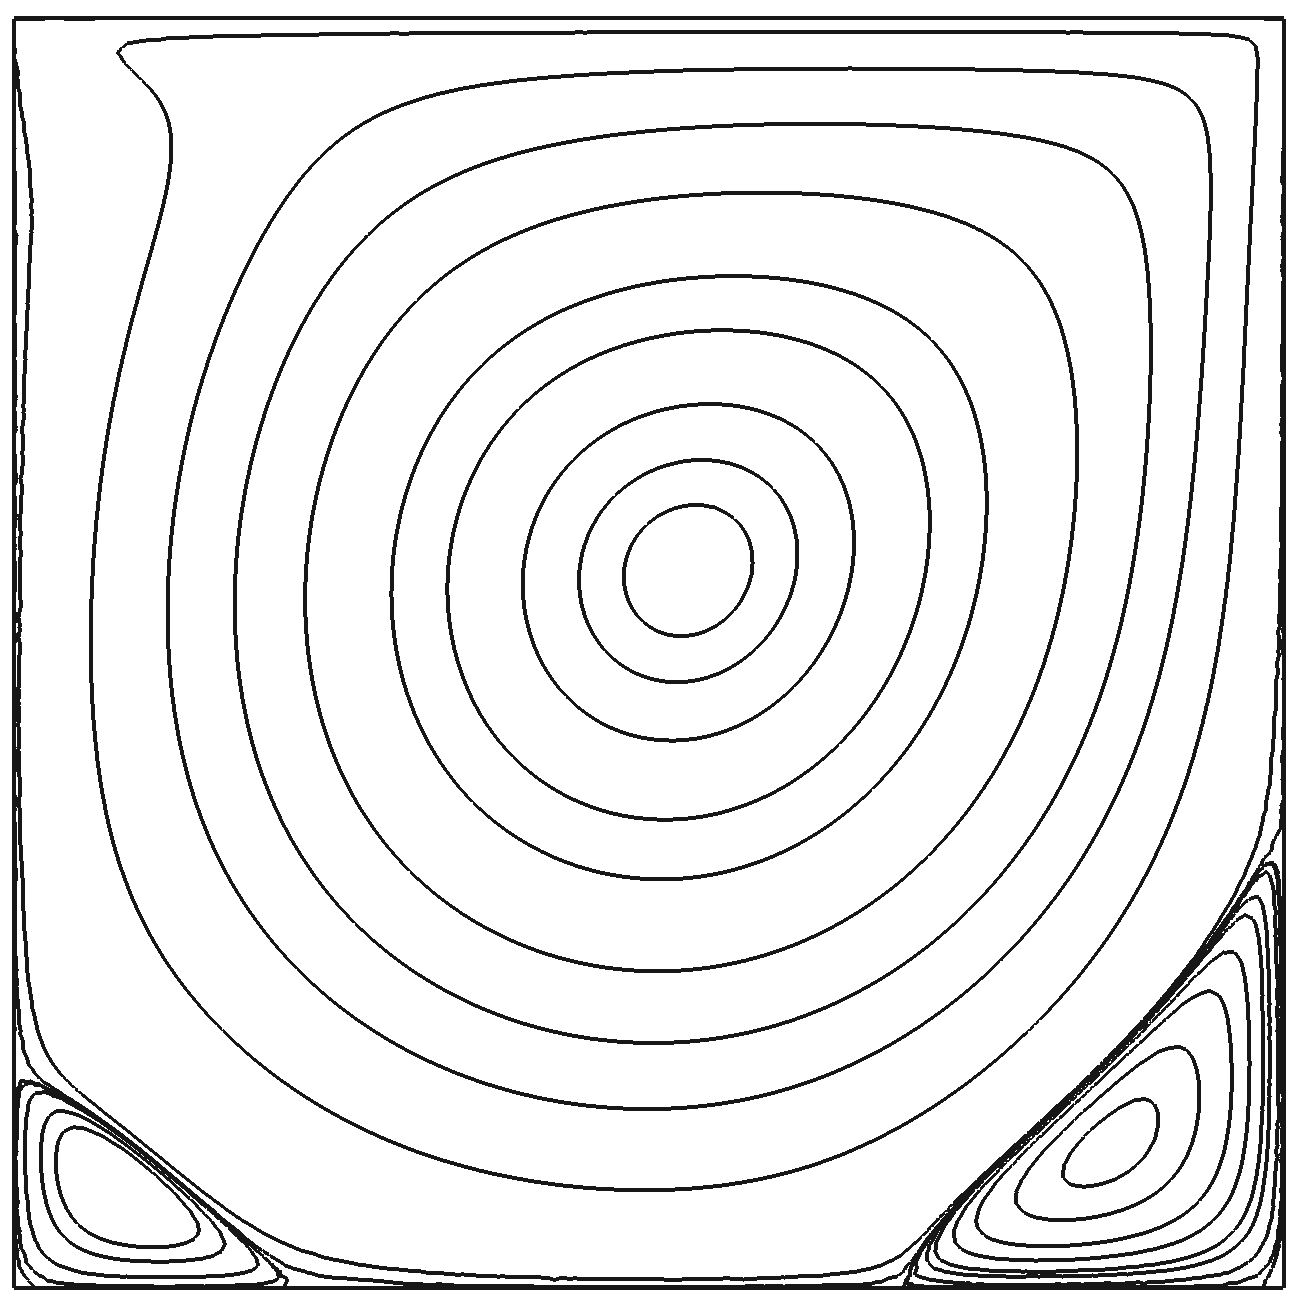
\includegraphics[width=7cm,clip]{examples_images/driven_cavity/driven_cavity_streamfunction.png}}
\subfigure{
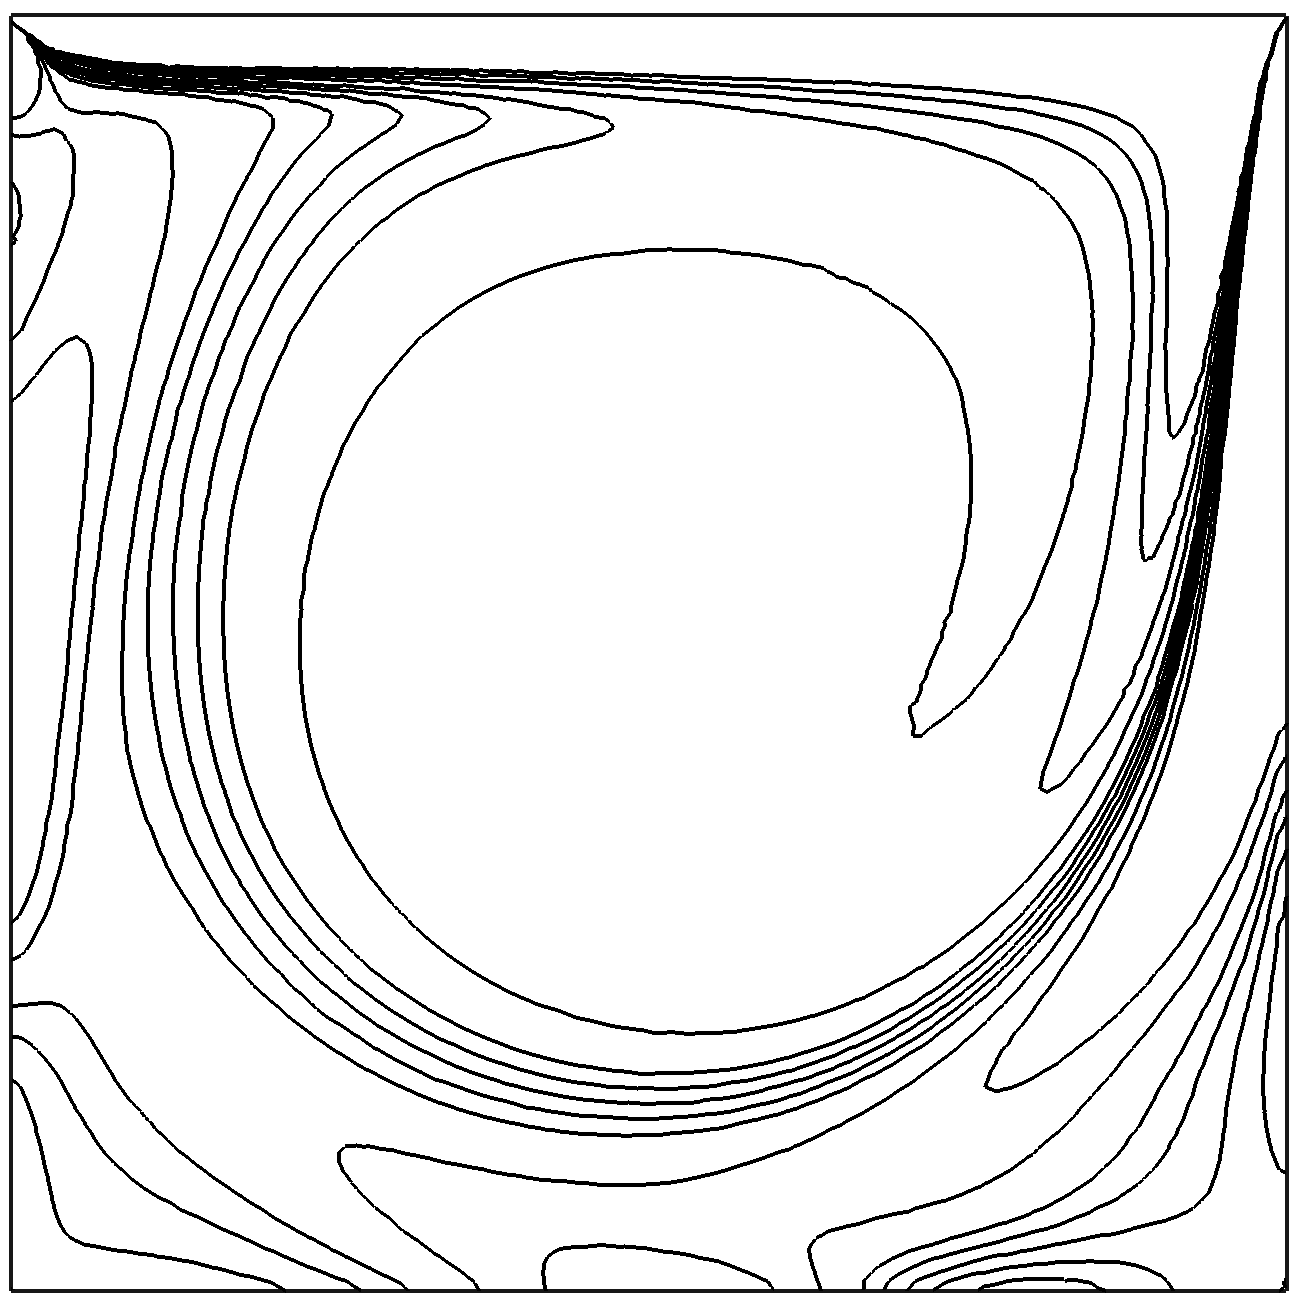
\includegraphics[width=7cm,clip]{examples_images/driven_cavity/driven_cavity_vorticity.png}}
\caption{Diagnostic fields from the lid-driven cavity problem at steady state at $1/128$ resolution.
Left: the streamfunction. Right: the vorticity. The contour levels are taken from those given by \cite{botella1998} in their tables
7 and 8.}
\label{fig:driven_cavity1}
\end{figure}


\subsection{Results}
Plots of the streamfunction and vorticity from the $h=1/128$ simulation are shown in figure \ref{fig:driven_cavity1}.
Observe the good qualititative agreement with \citep{botella1998,erturk2005,bruneau2006}. 
For a quantitative comaprison we take advantage of the tabulated benchmark data available in these papers.
Only a subset of these are computed: the $u$ velocity at a series of points along the line $x=0.5$ and the
$v$ velocity at a series of points along the line $y=0.5$ from \citep{erturk2005}, the same quantities at
different points along the same lines as well as the pressure along both the $x=0.5$ and $y=0.5$ lines from 
\citep{botella1998}, and the kinetic energy and the minimum streamfunction value from \citep{bruneau2006}.
The RMS difference in the case of the first six sets of benchmark data are taken with values extracted from 
the numerical solution, and the absolute difference taken in the final two. These eight error values are
defined as error1, \ldots error8 respectively and and plotted for the four mesh resolutions in figure 
\ref{fig:driven_cavity2}.
Second order spatial convergence can clearly be seen.
Adaptive refinement is not particularly advantageous for the problem at this reasonably low Reynolds number, but
yields significant improvements in efficiency at higher Reynolds number where boundary layers and
recirculating eddies are more dynamic, anisotropic and smaller in size compared to the entire domain.

\begin{figure}
\centering
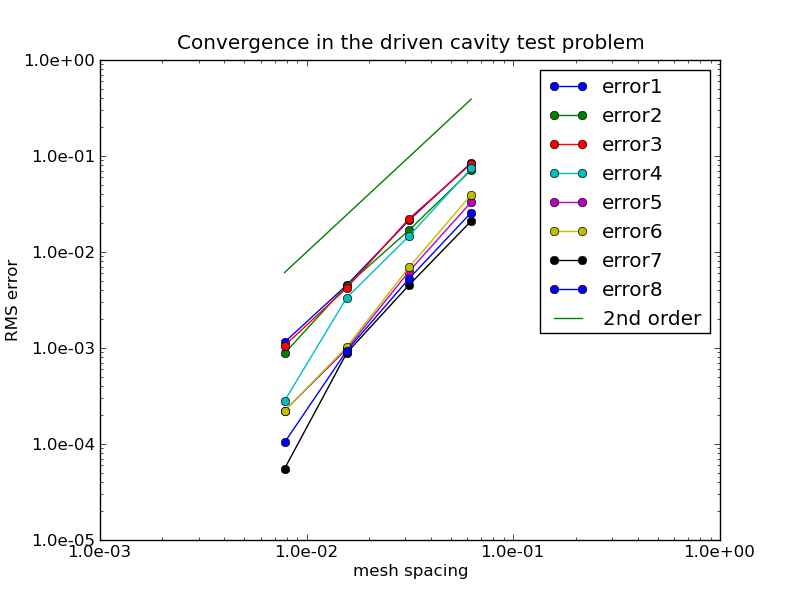
\includegraphics[width=10cm,clip]{examples_images/driven_cavity/driven_cavity_error_plot.png}
\caption{Convergence of the eight error metrics computed for the lid-driven cavity problem with mesh spacing. The eight
metrics are described in the text.}
\label{fig:driven_cavity2}
\end{figure}

\subsection{Exercises}
\begin{enumerate}
\item Examine the way that the $u=1$ lid condition is applied in the flml file. Why has it not been set as simply a constant?
Try changing it to a constant and see what happens to the errors that you achieve. [Hint: some people consider the "regularised" 
lid-driven cavity problem. Try finding some papers that discuss this, and update the boundary condition so it matches the 
regularised problem. Compare to benchmark data if you can find it].
\item The references given above include data from other Reynolds numbers. Try updating the problem set-up and the post-processing script which computes
the errors for a higher Reynolds number.
\item Try switching on mesh adaptivity (you will need to ensure that you have configured your \fluidity\ executable with \texttt{--enable-2d-adaptivity}). 
Test adapting based on different metrics, e.g. try weighting $u$, $v$ and $p$
differently and see what meshes you get. Try varying these weights as well as the maximum and minimum allowed element
sizes to see how they affect each other and the mesh that results. Can you get a metric that results in a lower
error for the same number of nodes compared to the fixed mesh (hint: it may be easier to achieve this at higher Reynolds numbers)?.
\end{enumerate}


%%%%%%%%%%%%%%%%%%%%%%%%%%%%%%%%%%%%%%%%%%%%%%%%%%%%%%%%%%%%%%%%%%%
%---------------------BACKWARD FACING STEP------------------------%
%%%%%%%%%%%%%%%%%%%%%%%%%%%%%%%%%%%%%%%%%%%%%%%%%%%%%%%%%%%%%%%%%%%

\section{Backward facing step}
\label{sect:backward_facing_step}


\subsection{Overview}
The backward-facing step is a classical CFD example and one of the most frequently selected
problems for simulating the separation and reattachment of turbulent flows.
It is also often used as a test problem for validating and benchmarking numerical codes.
At high Reynolds numbers and in three spatial dimensions the problem has substantial
computing requirements, this makes it an ideal HPC benchmark problem for use here.
In the context of ocean modelling flow separation is important
in large scale western boundary currents such as the Gulf Stream.

Accurate experimental results for a wide range of flow regimes exist
in 2D and 3D
(e.g. see \cite{armaly1983}) and the problem has several important flow
characteristics, such as the downstream length at which the flow reattaches
with the bottom of the domain. Results from \fluidity\ simulations at Reynolds number 150
are presented here.


\subsection{Configuration}
\subsubsection{Geometry: 3D}
A schematic of the domain is shown in figure \ref{Fig:Schematic3d}.
An inflow is imposed at the left hand boundary and encounters a step
down in the geometry. The region directly downstream of the step is
of particular interest in this problem. An outflow boundary is located at the
right hand end of the geometry.

Please note, this 3D example is intended to be run in parallel (see \ref{decomp_meshes_parallel}).
This is because the mesh must be fine enough, and the Reynolds number high enough, in order to
generate turbulence over the step and resolve its passage downstream. More information on running
Fluidity in parallel is found in \ref{sect:running_fluidity_in_parallel}.

In practice the example is run in a very similar way to the other examples.
To run in serial, the example is run in exactly the same way to the other examples, using
the commands \option{make preprocess}, \option{make run} and \option{make postprocess}.
To run in parallel with your chosen number of processors (\option{np}), using the command
\option{make preprocess NPROCS=np} creates a mesh and decomposes it into (\option{np}) parts, and
the command \option{make run NPROCS=np} runs \fluidity\ as (\option{np}) processes on (\option{np}) processors.
The command \option{make postprocess NPROCS=np} runs the parallel-specific data processing script.

\begin{figure}
\centering
\pdffig[width=12.0cm]{examples_images/backward_facing_step/backward_facing_step_3d-schematic}
\caption{Schematic of the domain for the three-dimensional flow past a backward facing step
problem.}
\label{Fig:Schematic3d}
\end{figure}

Following \cite{le1997} the length scales are given by: $L_x=30$, $L_i=10$, $L_y=4$, $h=1$, $L_z=6$,
so that $L_z-h=5$ and the expansion ratio is $L_z/(L_z-h)=1.2$.
The base of the domain is located at $z=0$, the inflow plane is given by $x=-10$ with the step
at $x=0$, and the back of the domain in the spanwise direction is given by $y=0$.

\subsubsection{Geometry: 2D}
A schematic of the domain, showing adaptive mesh refinement, is shown in figure \ref{Fig:Schematic2d}.
In the 2D case the expansion ratio is 2, and the upper boundary is treated as no-slip,
consistent with \cite{armaly1983}.

\begin{figure}
\centering
\pdffig[width=17.0cm]{examples_images/backward_facing_step/backward_facing_step_2d-mesh}
\caption{Schematic of the domain for the two-dimensional flow past a backward facing step
problem, showing adaptive mesh refinement.}
\label{Fig:Schematic2d}
\end{figure}


\subsubsection{Initial and boundary conditions: 3D}
In the 3D case, the inflow boundary condition at $x=-10$ is a log profile given by
\begin{equation*}
u(z) =
  \begin{cases}
    0.0 & \text{if } z-h \leq z_0 \\
    \frac{u_{\tau}}{\kappa} \log \left(\frac{z - h}{z_0}\right) & \text{if } z_0 < z-h
  \end{cases}
\end{equation*}

with parameters $u_{\tau} = 0.1$, $z_0 = 0.01$ and $\kappa = 0.41$.

%A plot of this inflow profile is given in figure \ref{Fig:Inflow}.
%\begin{figure}
%\centering
%\pdffig[width=8.0cm]{images/StepInflow.pdf}
%\caption{Inflow profile.}
%\label{Fig:Inflow}
%\end{figure}

No-normal flow, free-stress boundary conditions are applied at the upper and lateral
(spanwise) boundaries:
\begin{eqnarray*}
&&w=0,\quad \frac{\partial u}{\partial z} = \frac{\partial v}{\partial z} = 0 \quad\textrm{--- upper boundary},\\
&&v=0,\quad \frac{\partial u}{\partial z} = \frac{\partial w}{\partial z} = 0 \quad\textrm{--- lateral boundaries}.
\end{eqnarray*}

Free-stress boundary conditions are applied at the outflow boundary boundary:
\begin{equation*}
\frac{\partial u}{\partial x} = \frac{\partial v}{\partial x} = \frac{\partial w}{\partial x} = 0.
\end{equation*}

No-slip boundary conditions are applied at the bottom of the domain and at the step down:
\begin{equation*}
u=v=w=0.
\end{equation*}

\subsubsection{Initial and boundary conditions: 2D}
In the 2D case, the inlet velocity profile is a log profile extending from each wall to the midpoint, with the same parameters as the 3D example:
\begin{equation*}
u(z) =
  \begin{cases}
    0.0 & \text{if } (z-h) \leq z_0 \\
    \frac{u_{\tau}}{\kappa} \log \left(\frac{z - h}{z_0}\right) & \text{if } z_0 < (z-h) \leq 0.5 \\
    \frac{u_{\tau}}{\kappa} \log \left(\frac{2h - z}{z_0}\right) & \text{if } 0.5 < (z-h) \leq (2h-z_0) \\
    0.0 & \text{if } 2h-z_0 < (z-h)
  \end{cases}
\end{equation*}


\subsection{Results: 2D}
Three snapshots of the velocity magnitude from the benchmark run at $Re=150$
are shown in figure \ref{Fig:velo-magnitude-2d} at times 5, 10 and 50 seconds.
Vertical profiles of $\vec{u}$ at several points downstream of the step are shown
in figure \ref{Fig:UProfiles2d}. The reattachment point is clearly between $x/h=2$ and $x/h=4$.

One of the metrics most often considered for this test case is the point at which the
flow which separates from the step reattaches to the bottom of the domain.
The length downstream of the step at which this happens
has been found from laboratory experiments and direct numerical simulations and is considered a
sensitive measure of the quality of the numerical method. It is typically used to examine the impact
of turbulence parameterisations but here will be used to examine the use of mesh adaptivity
as well as the numerical method.

The reattachment length was defined here to be the length (normalised by step height $h$)
from the step at which the zero-contour of the $x$-component of $\vec{u}$ intersects with
the bottom boundary. This quantity was computed from $\vec{u}$
using the VTK library. For the simulation described, the reattachment
length was approximately 3.6 times the step height, which is consistent with \cite{armaly1983}.
The precise value for the reattachment length is dependent on exact configuration on the domain and inflow
conditions, and also strongly on the Reynolds number of the flow.

\begin{figure}
\centering
\subfigure{\pdffig[width=15.0cm]{examples_images/backward_facing_step/velo-magnitude-2d-5sec}}
\subfigure{\pdffig[width=15.0cm]{examples_images/backward_facing_step/velo-magnitude-2d-10sec}}
\subfigure{\pdffig[width=15.0cm]{examples_images/backward_facing_step/velo-magnitude-2d-50sec}}
\caption{Snapshots of the velocity magnitude from the 2D run at times 5, 10 and 50 time units
(top to bottom) into the simulation from the smaller benchmark run.
The evolution of the dynamics to steady state can be seen, in particular the downstream movement
of the streamline reattachment point (indicated by contours of $U=0$).}
\label{Fig:velo-magnitude-2d}
\end{figure}

\begin{figure}
\centering
\pdffig[width=17.0cm]{examples_images/backward_facing_step/velo_profiles_2d}
\caption{Streamwise velocity profiles from the 2D run at $x/h=0, 2, 4 \text{ and } 6$
downstream of the step, where $h=1$ is the step height. The converged solution is in red.
The recirculation region is indicated by negative velocity in figure (b).
It is clear that the reattachment point is between $x/h=2$ and $x/h=4$.}
\label{Fig:UProfiles2d}
\end{figure}


\subsection{Results: 3D}
Three snapshots of the velocity vectors are shown in figure \ref{Fig:velo-magnitude-3d}
at times 5, 10 and 50 seconds.
Vertical profiles of $\vec{u}$ at several points downstream of the step are shown in figure
\ref{Fig:UProfiles3d}, in which the velocity data has been averaged across the span of the domain
to obtain quasi-2D data. The reattachment point is clearly between $x/h=6$ and $x/h=10$.
In fact the flow reattaches at $x/h \approx 8.3$.


\begin{figure}
\centering
\subfigure{\pdffig[width=15.0cm]{examples_images/backward_facing_step/velo-magnitude-3d-5sec}}
\subfigure{\pdffig[width=15.0cm]{examples_images/backward_facing_step/velo-magnitude-3d-10sec}}
\subfigure{\pdffig[width=15.0cm]{examples_images/backward_facing_step/velo-magnitude-3d-50sec}}
\caption{From top to bottom: vertical plane cuts through the 3D domain showing
the velocity magnitude at times 5, 25 and 50 time units.
The evolution of the dynamics to steady state can be seen, in particular the downstream movement
of the streamline reattachment point (indicated by contours of $U=0$).}
\label{Fig:velo-magnitude-3d}
\end{figure}

\begin{figure}
\centering
\pdffig[width=17.0cm]{examples_images/backward_facing_step/velo_profiles_3d}
\caption{Streamwise velocity profiles from the 3d run at $x/h=4, 6, 10 \text{ and } 19$
downstream of the step, where $h=1$ is the step height. The converged solution is in red.
The recirculation region is indicated by the negative velocity in figure (b).
It is clear that the flow reattaches between $x/h>6 \text{ and } 10$.}
\label{Fig:UProfiles3d}
\end{figure}


%As this is a highly turbulent problem, making quantitative comparisons of
%individual snapshots is impossible. However, time-averaged quantities are of diagnostic interest.
%Figure \ref{Fig:TimeAverage} shows 3 snapshots of the $u$ component of velocity from the large
%benchmark run and a time
%averaged field. The removal of fluctuating components in the velocity field can be seen.

%\begin{figure}
%\centering
%\subfigure{\pdffig[width=15.0cm]{images/Velocity1.pdf}}
%\subfigure{\pdffig[width=15.0cm]{images/Velocity33.pdf}}
%\subfigure{\pdffig[width=15.0cm]{images/Velocity64.pdf}}
%\subfigure{\pdffig[width=15.0cm]{images/VelocityAverage.pdf}}
%\caption{Snapshots of the $u$ velocity components at three time slices (top three frames) and the
%average field from 64 input snapshots spaced equally between times 70 and 102 (bottom).
%Contours are displayed at the $-0.05$, $0.0$, $0.05$, $0.1$, $0.5$ and $1.0$ levels.}
%\label{Fig:TimeAverage}
%\end{figure}



A more rigorous analysis would involve
repeating the experiment for a range of Reynolds numbers and comparing the reattachment
length of multiple model runs.
%It may be seen that pseudo-supermeshing is an efficient
%method to produce a common mesh suitable for the interpolation of fields from multiple
%meshes, such as is necessary in time-averaging.

%%%%%%%%%%%%%%%%%%%%%%%%%%%%% %%%%%%%%%%%%%%%%%%%%%%%%%%%%%%%%%%%%%
%----------------------Sphere------------------------------------%
%%%%%%%%%%%%%%%%%%%%%%%%%%%%%%%%%%%%%%%%%%%%%%%%%%%%%%%%%%%%%%%%%%%

\section{Flow past a sphere: drag calculation}
\label{sect:flow_past_sphere}
\subsection{Overview}
In this validation test uniform flow past an isolated sphere is simulated
and the drag on the sphere is calculated and compared to a curve optimised
to fit a large amount of experimental data.

\subsection{Configuration}
The sphere is of unit diameter centred at the origin. The entire domain is
the cuboid defined by $-10\le x\le 20$, $-10\le y\le 10$, $-10\le z\le 10$.
GiD is used to mesh the initial geometry.

The unsteady momentum equations with nonlinear advection and viscous terms
along with the incompressibility constraint are solved. Free slip velocity
boundary conditions are applied at the four lateral boundaries, $u=1$, $v=w=0$ is
applied at the inflow boundary $x=-10$, and a free stress boundary condition
applied to the outflow at $x=20$. 

A series of Reynolds numbers in the range
$Re\in [1,1000]$ are considered. The problem is run for a long enough
period that the low Reynolds number simulations reach steady state, and the
higher Reynolds number runs long enough that a wake develops behind the
sphere and boundary layers on the sphere are formed.  This is deemed
sufficient for the purposes of this test; the example is to demonstrate
how such a problem would be set up, not conduct an in-depth 
investigation of the physics of this problem.

Here an unstructured
tetrahedral mesh is used along with mesh adaptivity. 
Figure \ref{fig:flow_past_sphere_2} shows a snapshot of the
mesh and velocity vectors taken from a Reynolds number 1000 simulation. The
mesh can be seen to be resolving the wake and the boundary layers on the
sphere with enhanced anisotropic resolution. At higher Reynolds numbers the
dynamics become more complex and if a full numerical study was being
conducted here more care would be taken is the choice of mesh optimisation
parameters and the use of averaged values from simulations allowed to run
for longer periods. The drag coefficient is calculated from
\begin{equation}
C_D = \frac{F_x}{\frac{1}{2}\rho u_0^2 A},\qquad F_x = \int_S (n_xp - n_i\tau_{ix})\;dS,
\label{eqn:drag_coeff}
\end{equation}
where $\rho$ is the density, taken here to be unity; 
$u_0$ is the inflow velocity, here unity; 
and $A$ is the cross-sectional area of the sphere, here $\pi^2/4$. 
$F_x$ is the force 
exerted on the sphere in the free stream direction;
$S$ signifies the surface of the sphere; $n$ is the 
unit outward pointing normal to the sphere 
($n_x$ is the $x$-component and $n_i$ the $i^{\textrm{th}}$ 
component, here summation over repeated indices is assumed); 
$p$ is the pressure and $\tau$ is the stress tensor;
see \citet{panton2006}.

\begin{figure}
\centering
\subfigure{
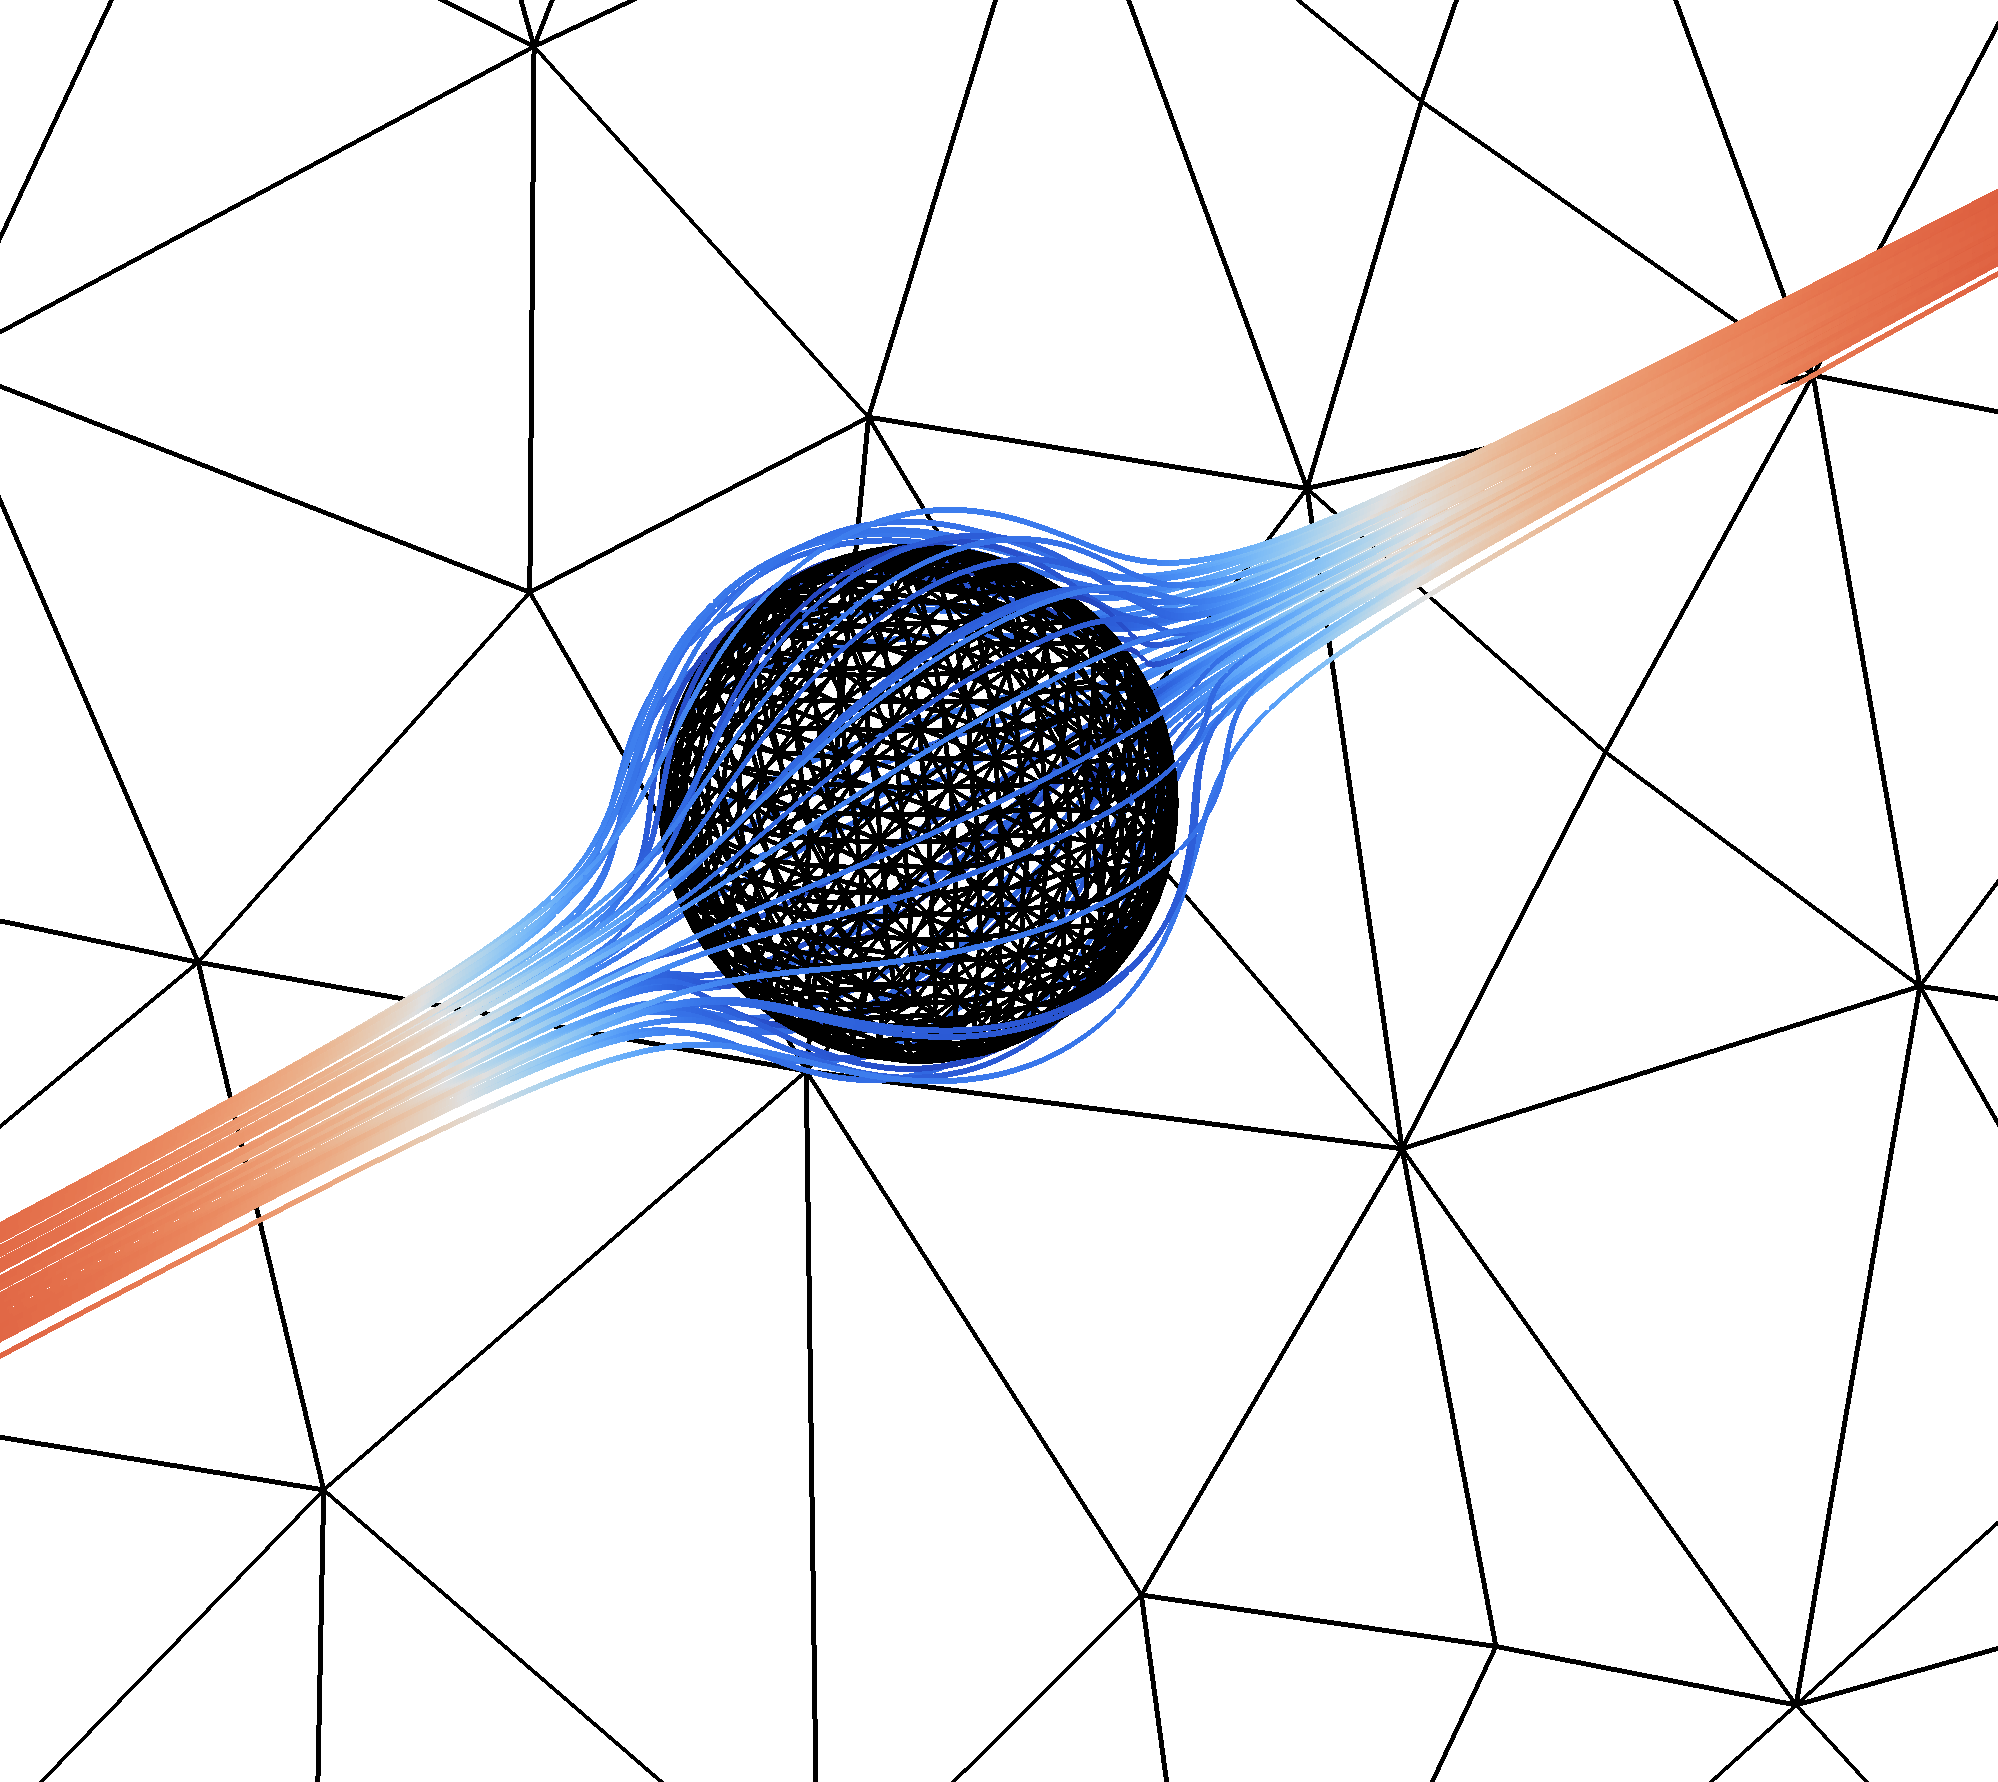
\includegraphics[width=6cm,clip]{examples_images/flow_past_sphere/sphere-Re1-streamlines.png}}
\subfigure{
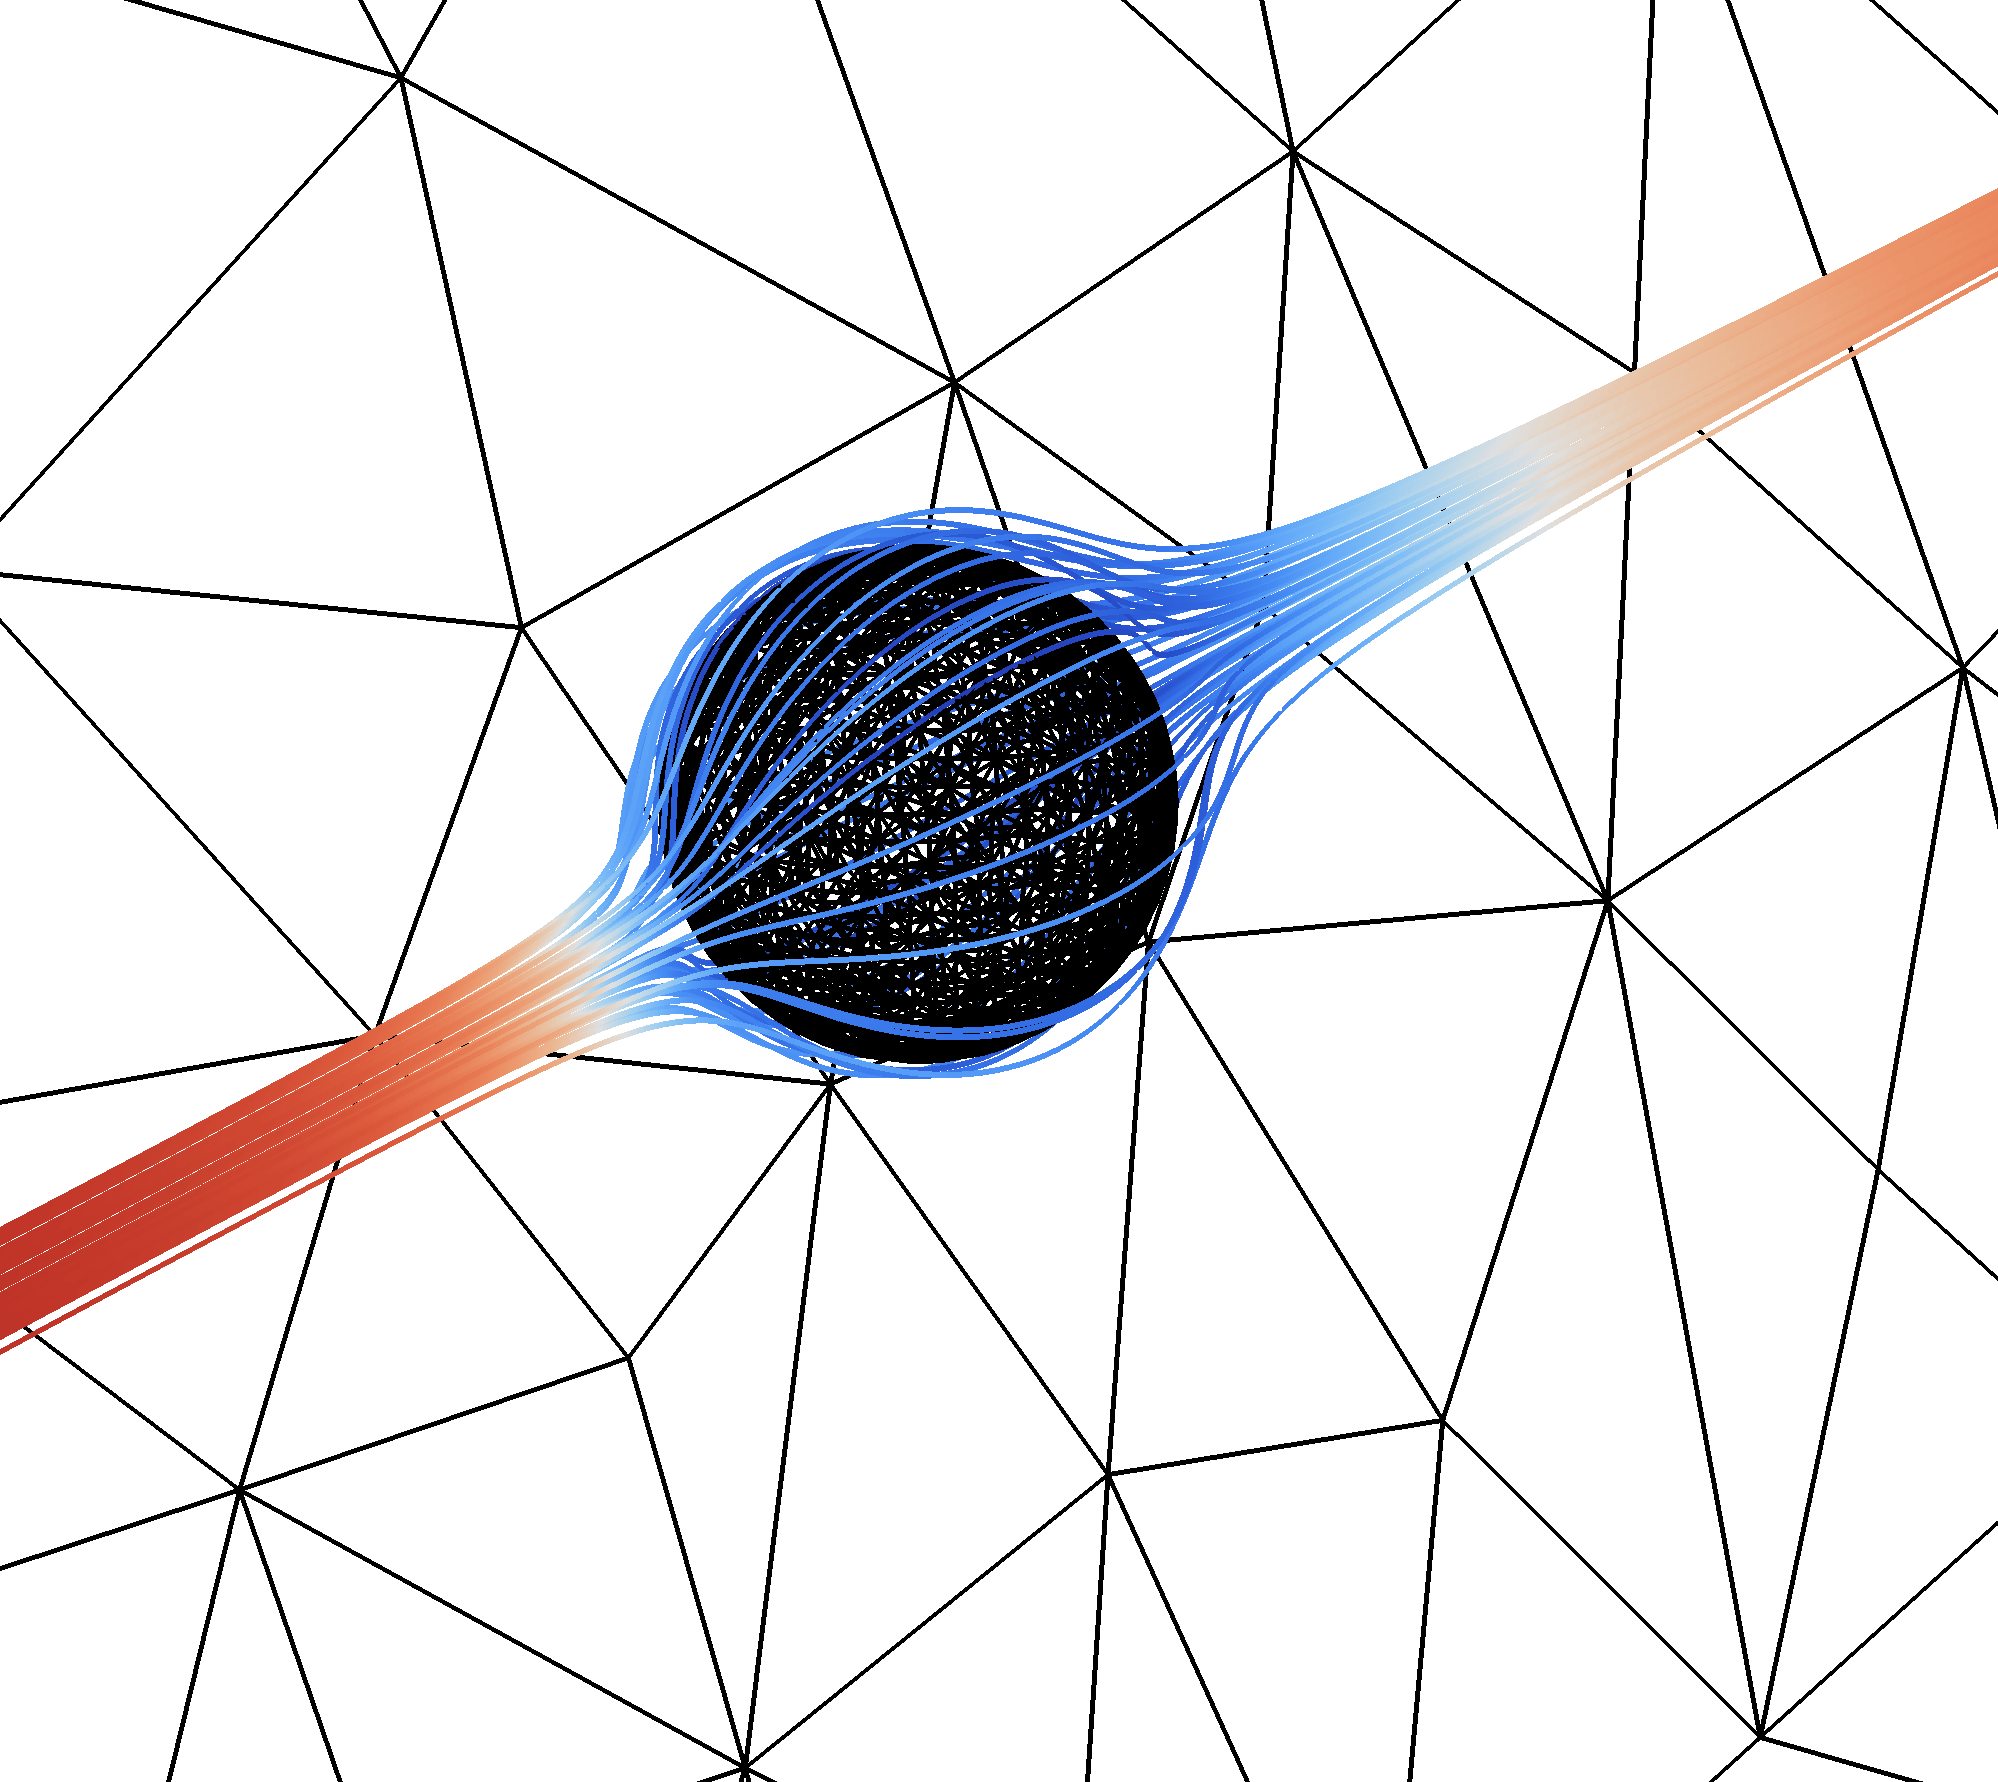
\includegraphics[width=6cm,clip]{examples_images/flow_past_sphere/sphere-Re10-streamlines.png}}
\subfigure{
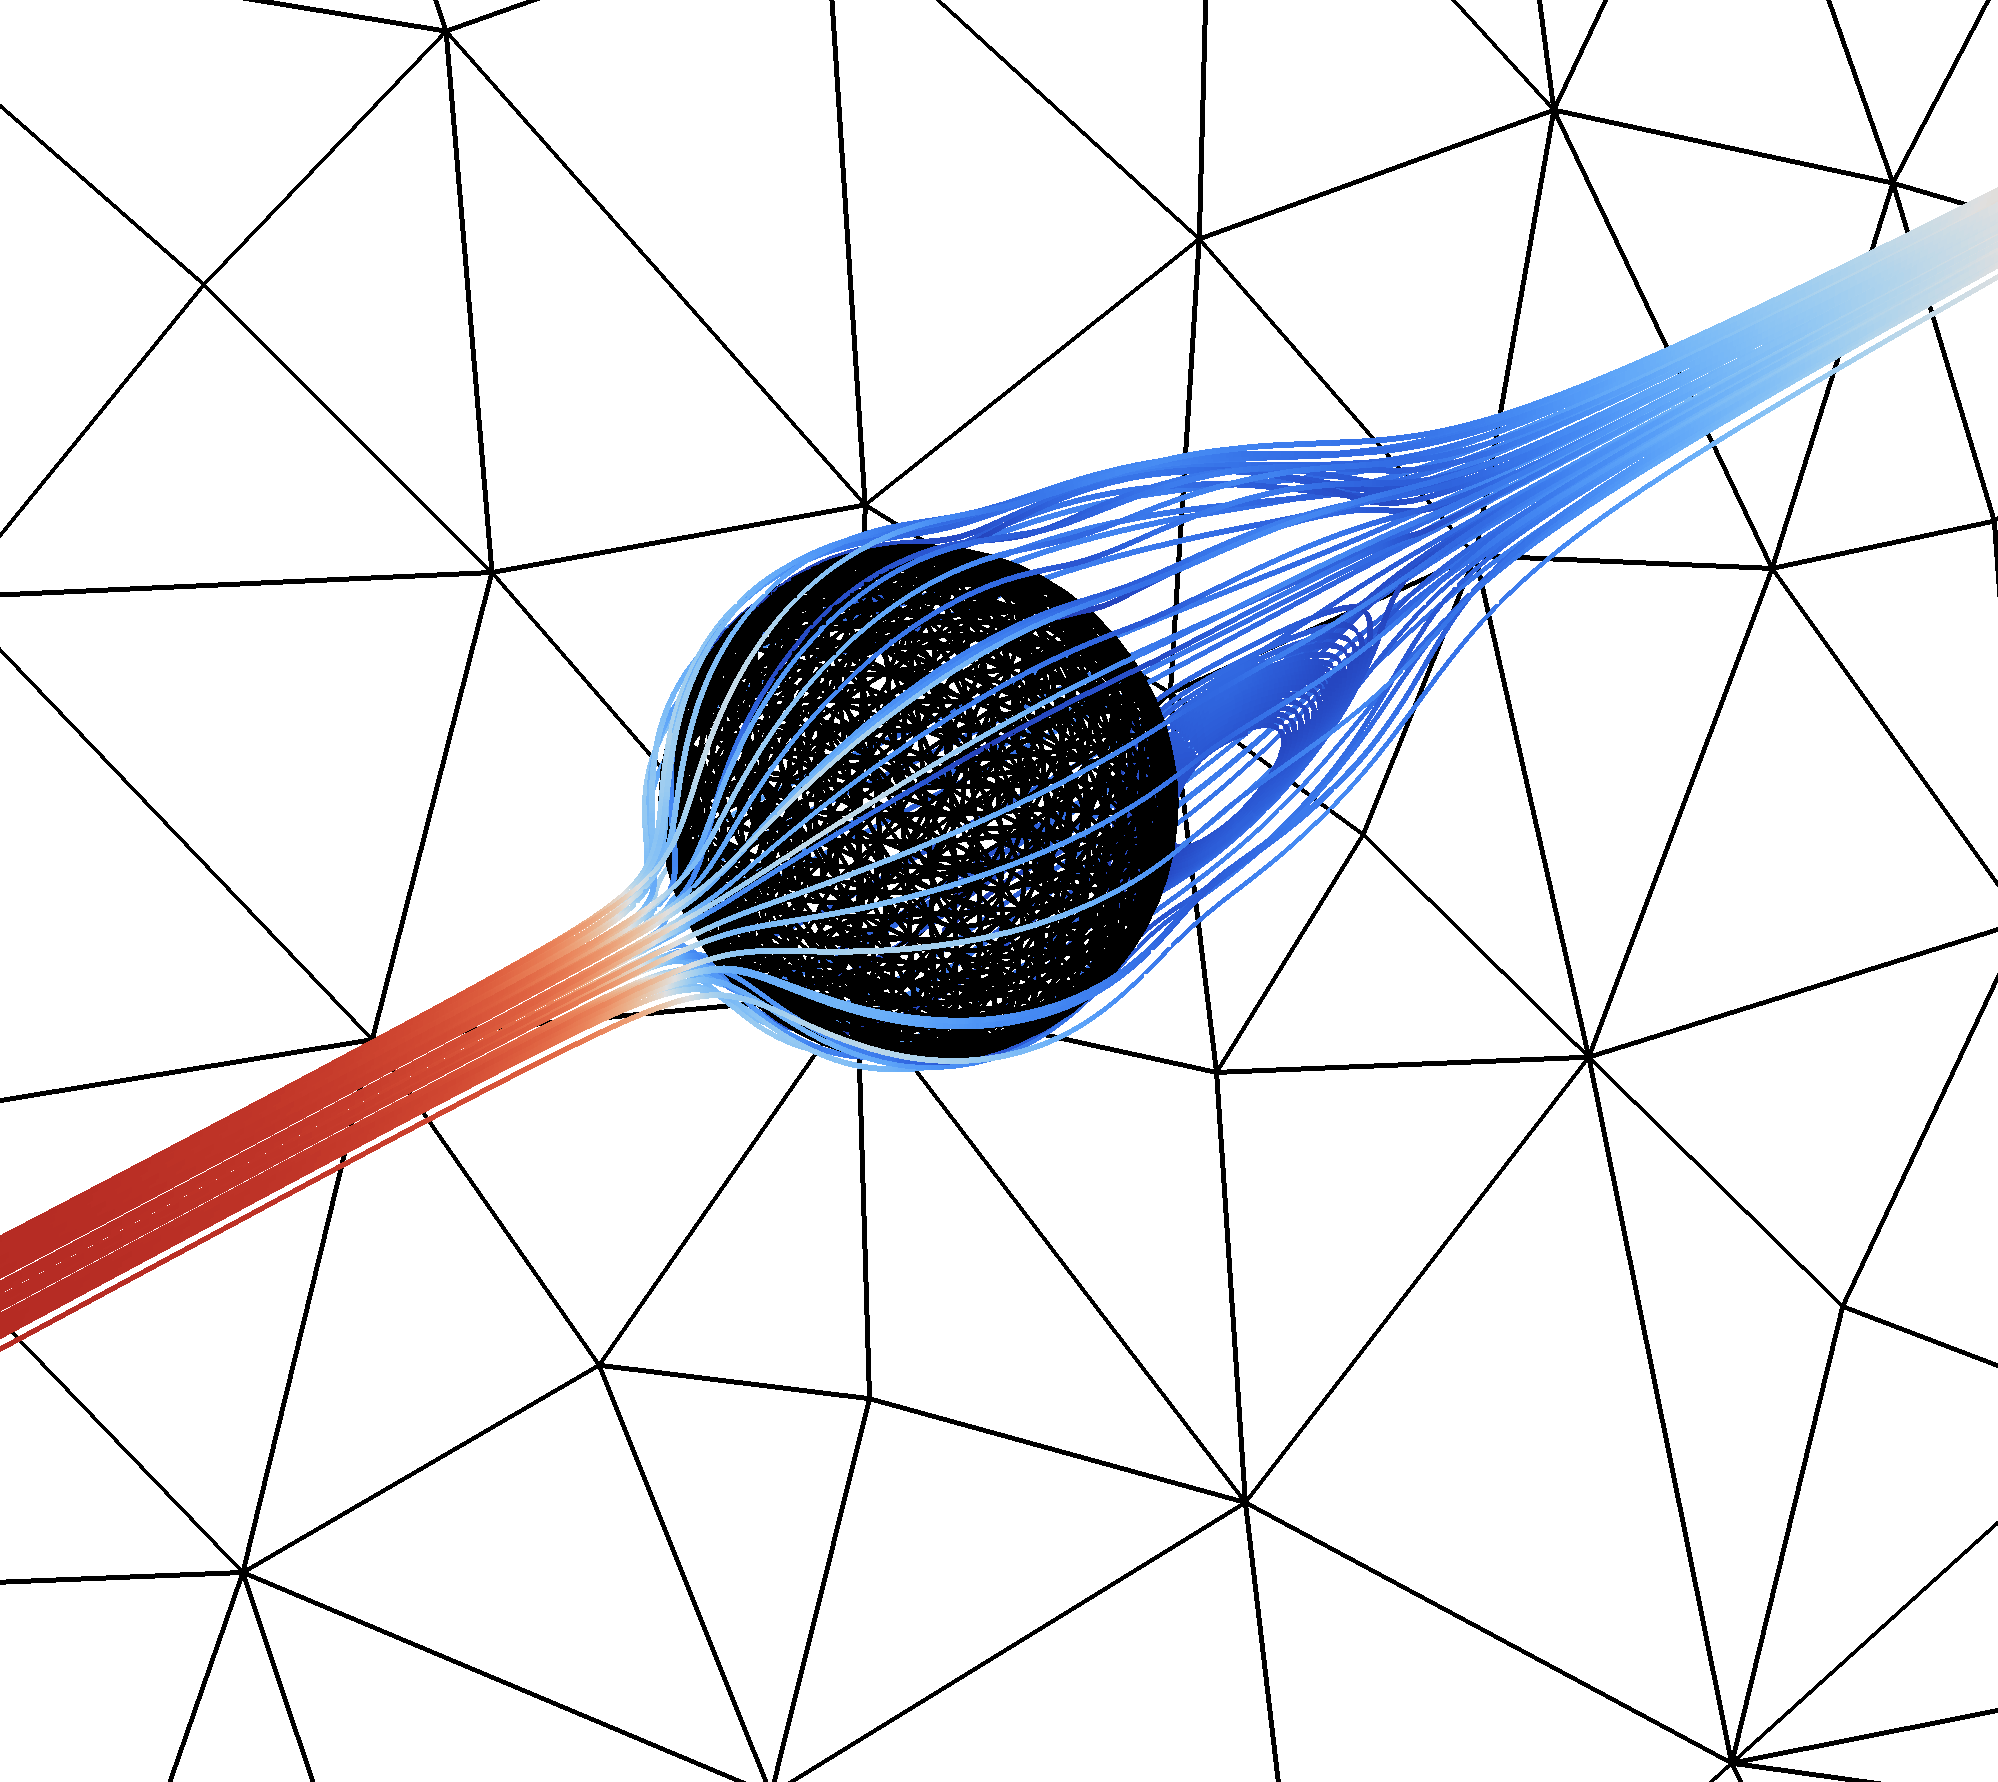
\includegraphics[width=6cm,clip]{examples_images/flow_past_sphere/sphere-Re100-streamlines.png}}
\subfigure{
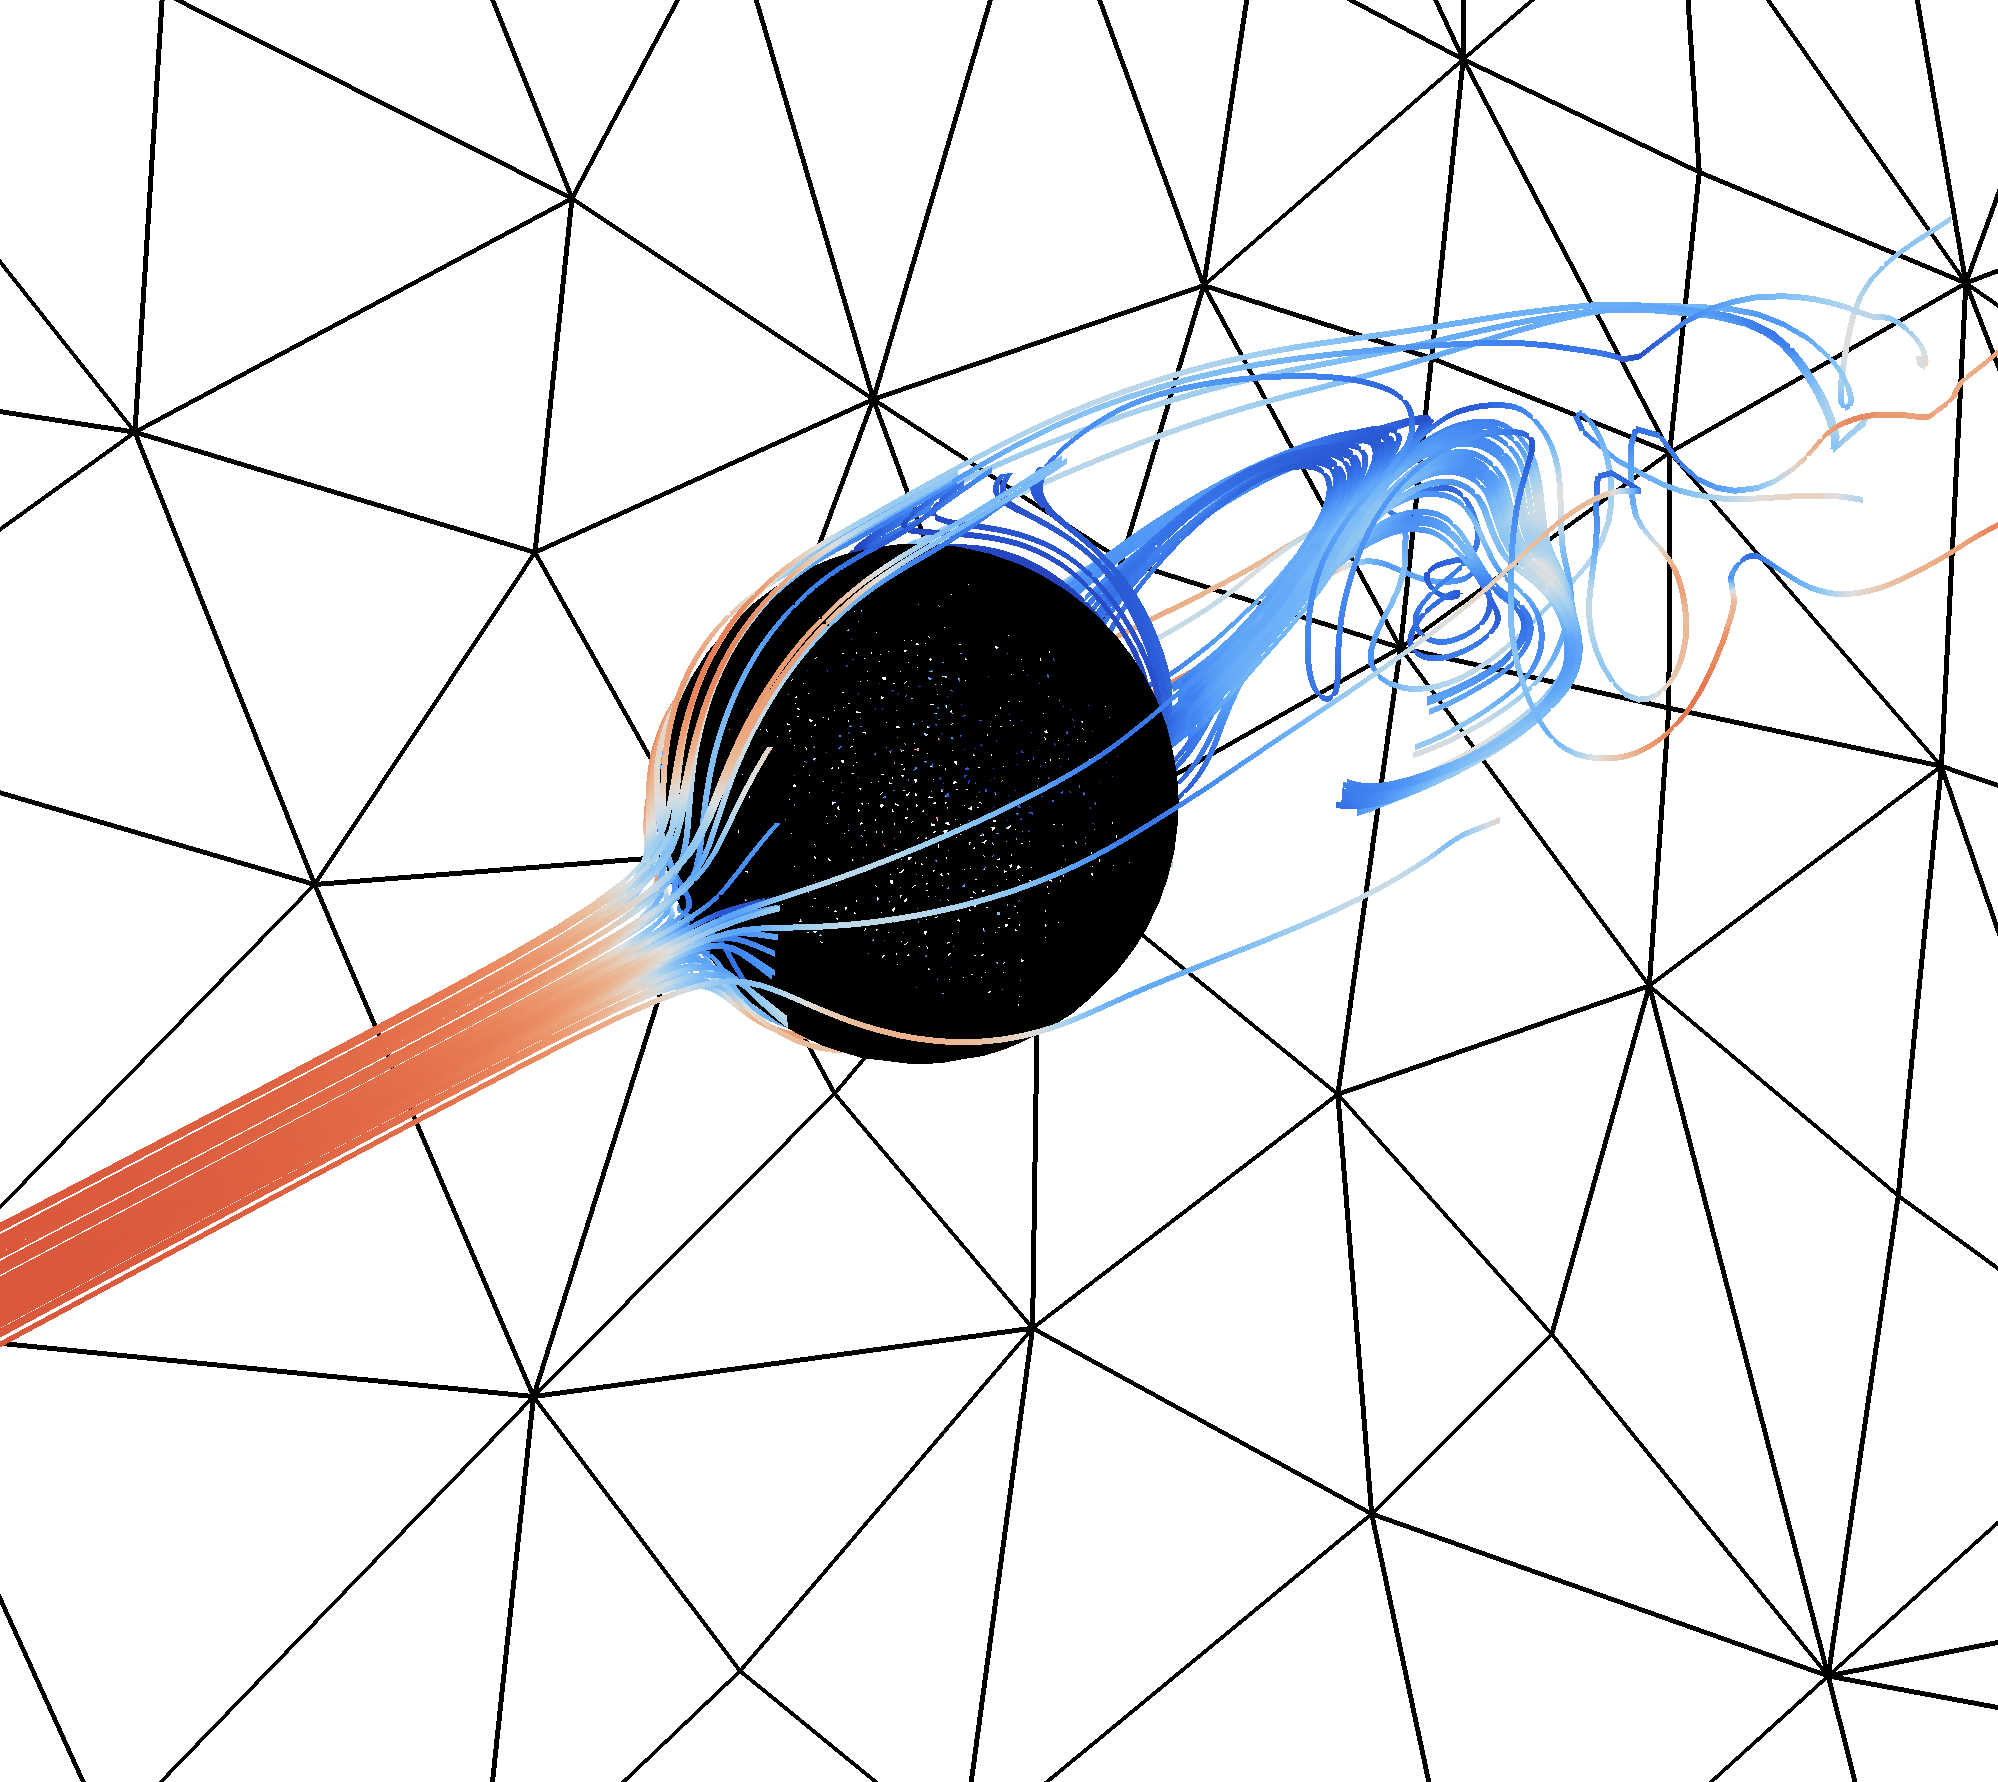
\includegraphics[width=6cm,clip]{examples_images/flow_past_sphere/sphere-Re1000-streamlines.png}}
\caption{Streamlines and surface mesh in the flow past the sphere example. Top-left to bottom-right
show results from Reynolds numbers $Re=1,10,100,1000$.}
\label{fig:flow_past_sphere_1}
\end{figure}


\begin{figure}
\centering
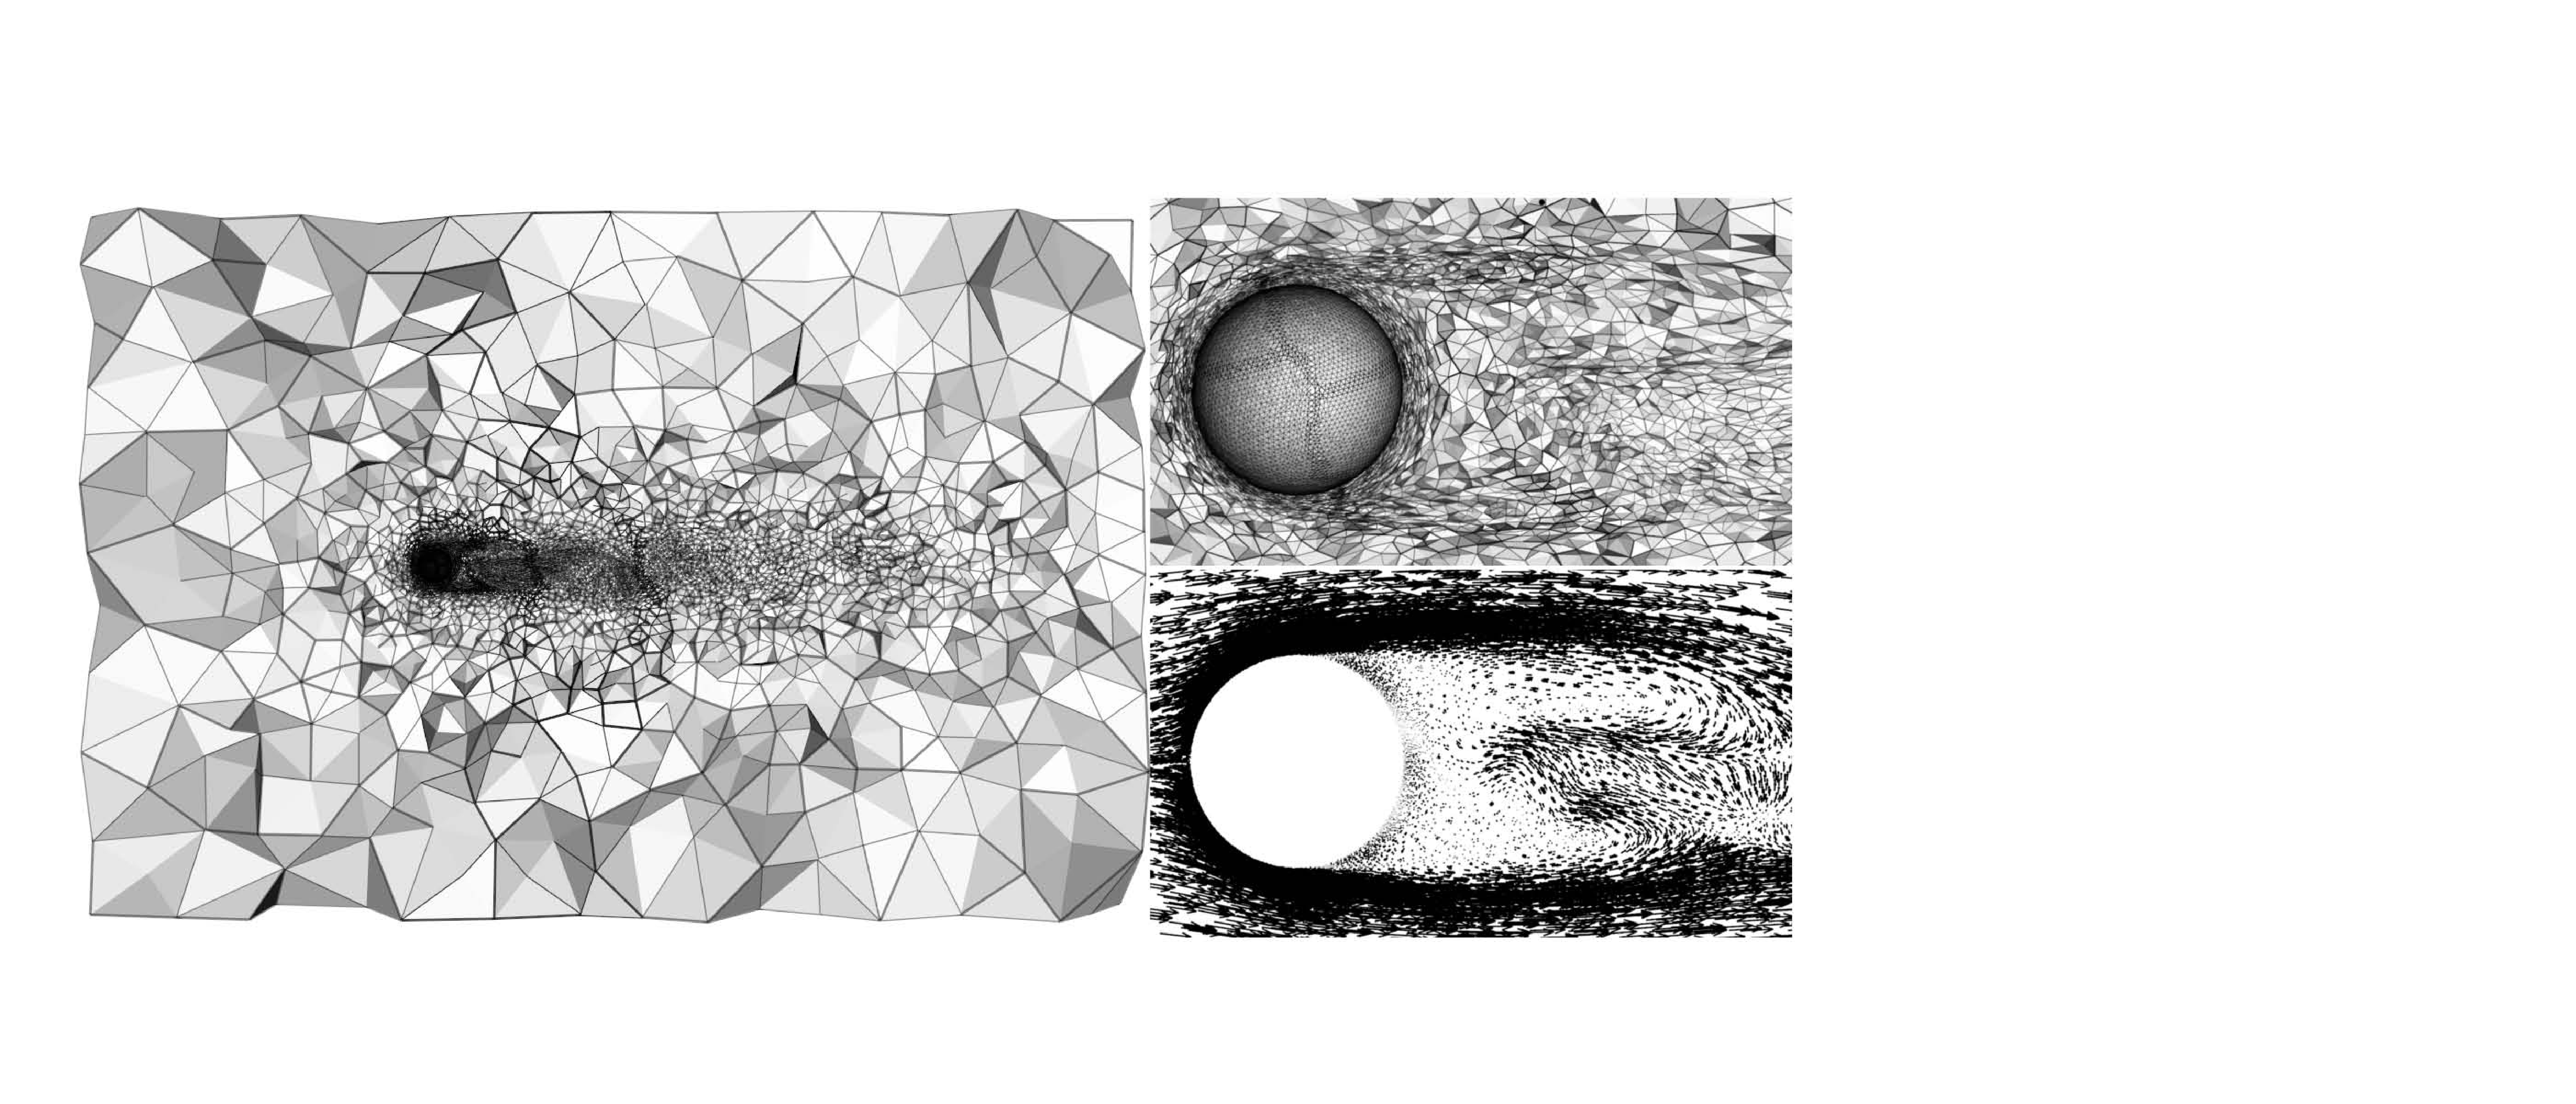
\includegraphics[width=15cm,clip]{examples_images/flow_past_sphere/sphere-Re1000-combined.pdf}
\caption{Details of the mesh and flow at $Re=1000$.}
\label{fig:flow_past_sphere_2}
\end{figure}

\subsection{Results}
Figure \ref{fig:flow_past_sphere_1} shows streamlines close to the sphere and the surface mesh.
The mesh can be seen to be much finer on the sphere compares to the far wall seen in the background.
This is empahsised in figure \ref{fig:flow_past_sphere_2} where a more detailed plot of the mesh (with
half of the domain removed) over the whole domain and close to the sphere, and the velocity vectors
close to the sphere are shown.

Figure \ref{fig:flow_past_sphere_3} shows a comparison between the computed drag coefficient with
a correlation (to a large amount of laboratory data) taken from \citet{brown2003}:
\begin{equation}
C_D = \frac{24}{Re}\left(1+0.15Re^{0.681}\right) + \frac{0.407}{1+\frac{8710}{Re}}.
\label{eqn:sphere_drag_corr}
\end{equation}
Excellent agreement can be seen at the range of Reynolds numbers tested in this exercise.


\begin{figure}
\centering
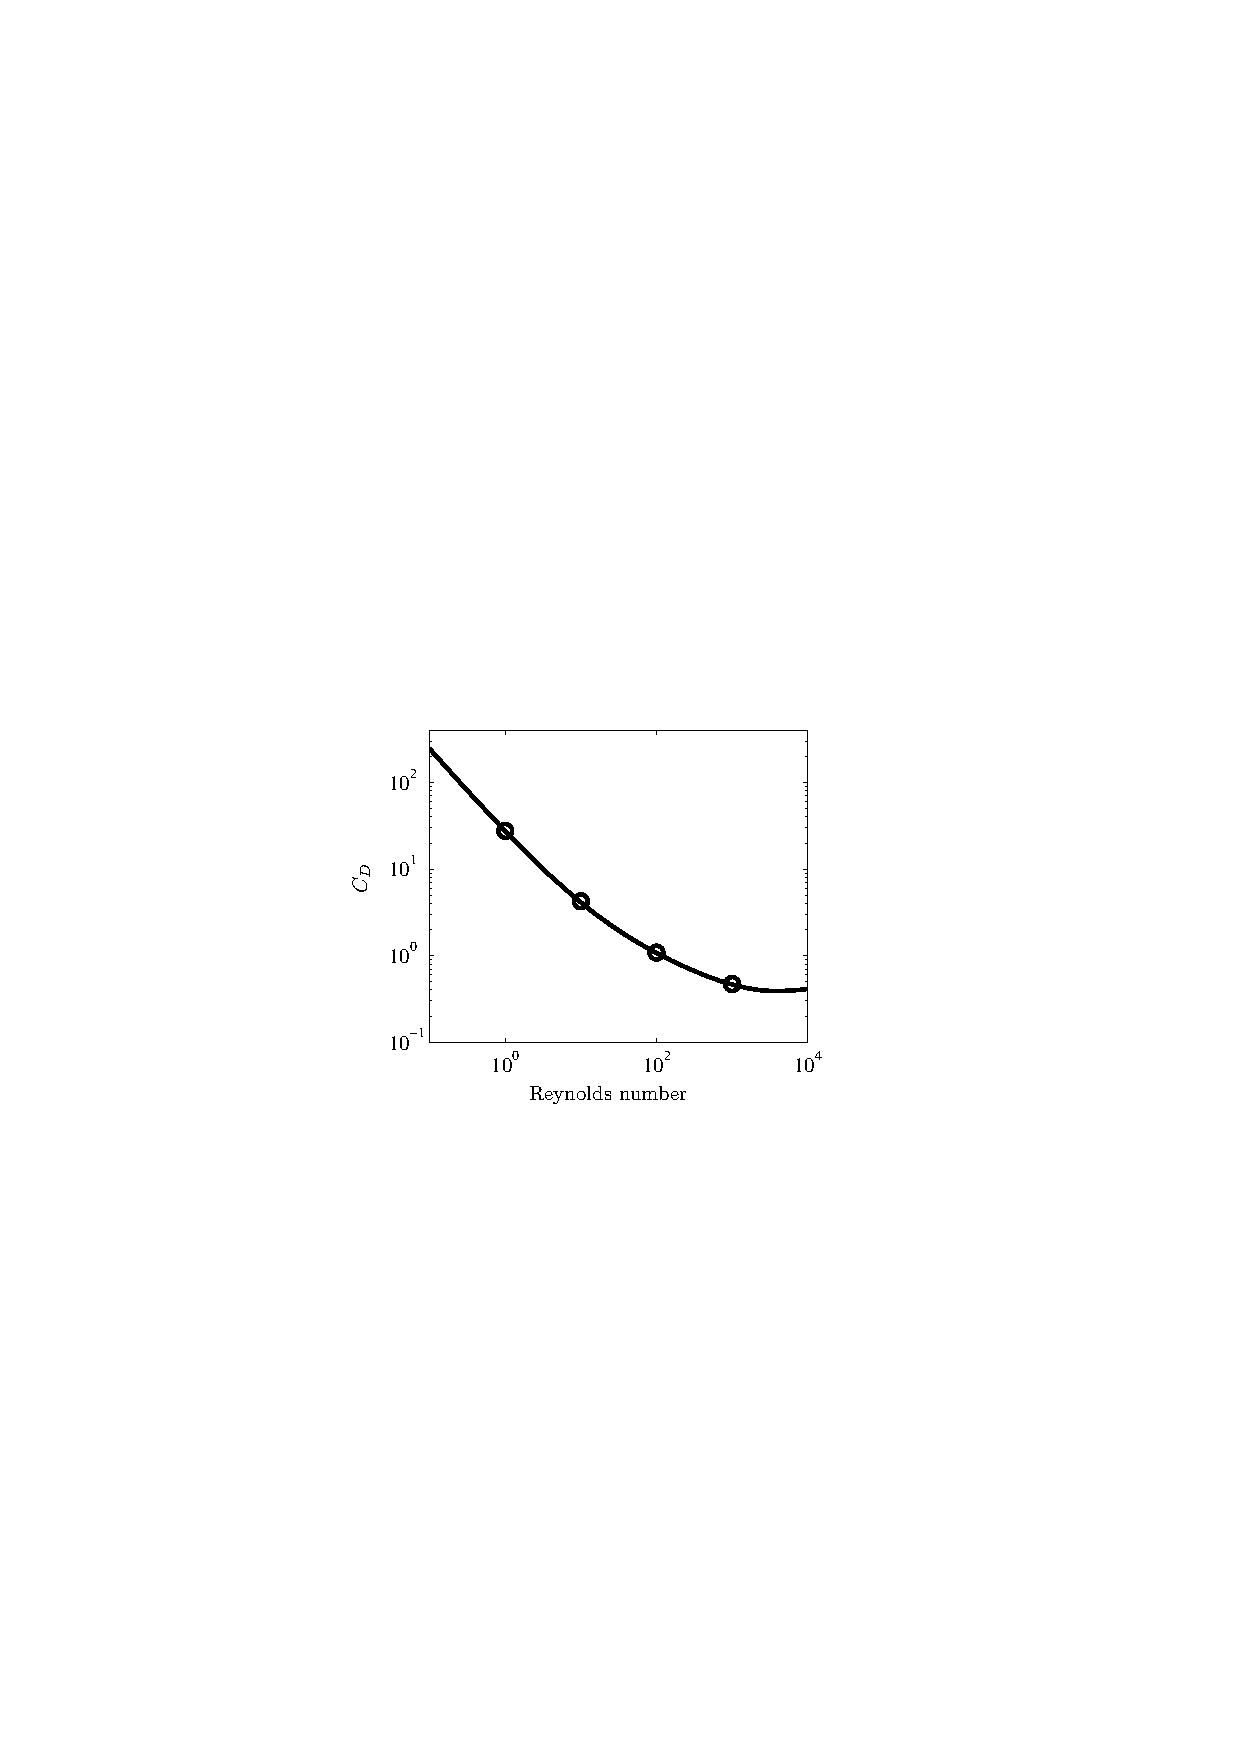
\includegraphics[width=8cm,clip]{examples_images/flow_past_sphere/Sphere_Drag.pdf}
\caption{Comparison between the numerically calculated drag coefficients ($C_D$, circles) and the correlation \eqref{eqn:sphere_drag_corr} (solid line)
for $Re=1,10,100,1000$.}
\label{fig:flow_past_sphere_3}
\end{figure}



\subsection{Exercises}
\begin{enumerate}
\item We actually compute the (vector) force on the sphere and output this to the stat file. This can then be converted to the drag coefficient 
via \eqref{eqn:drag_coeff}. Write a Python function to do this conversion and the error from the correlation \eqref{eqn:sphere_drag_corr}.
\item Try varying some of the discretisation and adaptivity parameters to see what the impact on the accuracy of the
calculated drag is.
\item Try changing the shape of the object, e.g. benchmark data is also available for flow past a cylinder \citep{schafer1996}.
\end{enumerate}


%%%%%%%%%%%%%%%%%%%%%%%%%%%%% %%%%%%%%%%%%%%%%%%%%%%%%%%%%%%%%%%%%%
%----------------------CHANNEL------------------------------------%
%%%%%%%%%%%%%%%%%%%%%%%%%%%%%%%%%%%%%%%%%%%%%%%%%%%%%%%%%%%%%%%%%%%

\section{Rotating periodic channel}
\label{sect:periodic_channel}

\subsection{Overview}

This problem provides a convergence test for the \PoDGPt\ element pair.
Utilising almost all the terms of the incompressible Navier-Stokes equations
in two dimensions.

The domain is a unit square which is periodic in the zonal direction. The
North and South boundaries are zero slip (i.e. $\vec{u}=0$). The remaining
parameters are as follows:

\begin{tabular}{lll}
  Coriolis parameter & $f$ & $1$ \\
  Viscosity & $\nu$ & $1$ 
\end{tabular}

The flow is driven by a velocity source term:
\begin{equation}
  \vec{F}=
  \begin{bmatrix}
    y^3 \\
    0
  \end{bmatrix}
\end{equation}

So the whole system of equations becomes:
\begin{gather}
  \ppt{u}+u\ppt[x]{u}-v=-\grad p + \grad^2 u +y^3\\
  \ppt{v}+v\ppt[y]{v}+u=-\grad p + \grad^2 v\\
  \div\vec{u}=0
\end{gather}

This system has a steady solution at:
\begin{gather}
  \vec{u}=
  \begin{bmatrix}
    \frac{1}{20}(y-y^5)\\
    0
  \end{bmatrix}\\
  p=\frac{1}{120}y^6-\frac{1}{40}y^2+C
\end{gather}
Where $C$ is an arbitrary constant resulting from the use of Dirichlet
boundary conditions on both the domain boundaries.

\subsection{Results}

Since the maximum velocity in the domain is approximately 0.025, the
Reynolds number for this solution is much smaller than 1 so the flow is
safely within the laminar regime and will remain steady. Figure
\ref{fig:periodic_channel}\ shows the forcing term for velocity and the
analytic solutions for velocity and pressure.


\begin{figure}[htbp]
  \centering
  \onlypdf{\begin{pdfdisplay}}
    \psfrag{u source}{$\vec{u}$ source}
    \psfrag{u solution}{$\vec{u}$ solution}
    \psfrag{p solution}{$p$ solution}
    \psfrag{0}{0}
    \psfrag{0.2}{0.2}
    \psfrag{0.4}{0.4}
    \psfrag{0.5}{0.5}
    \psfrag{0.2}{0.6}
    \psfrag{0.8}{0.8}
    \psfrag{1}{1}
    \psfrag{y}{$y$}
    \psfrag{-0.01}{-0.01}
    \psfrag{-0.02}{-0.02}
    \psfrag{0.01}{0.01}
    \psfrag{0.02}{0.02}
    \psfrag{0.03}{0.03}
    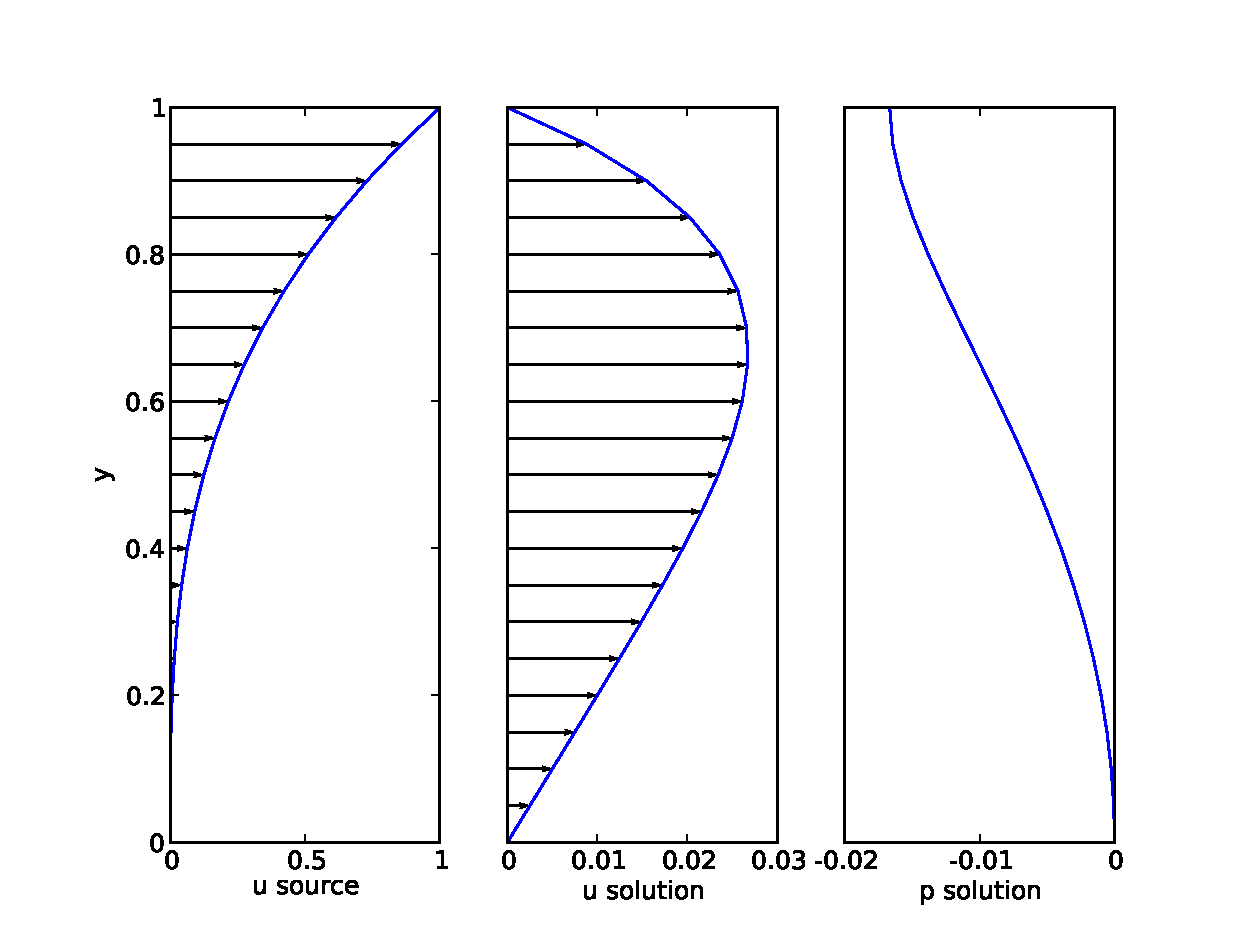
\includegraphics[width=1.1\textwidth]{examples_images/rotating_channel/analytic_solution.eps}
  \onlypdf{\end{pdfdisplay}}
  \caption{Velocity forcing term and analytic solutions for velocity and
    pressure for the rotating periodic channel test case. Note that each of
    these quantities is constant in the $x$ direction.}
  \label{fig:periodic_channel}
\end{figure}

The convergence test is conducted by repeating this simulation on unstructured meshes
with typical resolution $1/4$, $1/8$, $1/16$, $1/32$, $1/64$. The results
are then compared to the analytic solution. In the case of pressure, the
answer is translated to account for the arbitrary constant. Figure
\ref{fig:periodic_channel_error}\ shows the $\textrm{L}^2$ error for
velocity and pressure. It is apparent that both quantities converge at
second order.

\begin{figure}[htbp]
  \centering
  \onlypdf{\begin{pdfdisplay}}
    \psfrag{u error}{$\vec{u}$ error}
    \psfrag{p error}{$p$ error}
    \psfrag{O\(dx^2\)}{$O(\d x^2)$}
    \psfrag{dx}{$\d x$}
    \psfrag{1.0e+00}{\small\hspace{1em}$1$}
    \psfrag{1.0e-01}{\small\hspace{1em}$10^{-1}$}
    \psfrag{1.0e-02}{\small\hspace{1em}$10^{-2}$}
    \psfrag{1.0e-03}{\small\hspace{1em}$10^{-3}$}
    \psfrag{1.0e-04}{\small\hspace{1em}$10^{-4}$}
    \psfrag{1.0e-05}{\small\hspace{1em}$10^{-5}$}
    \psfrag{1.0e-06}{\small\hspace{1em}$10^{-6}$}
    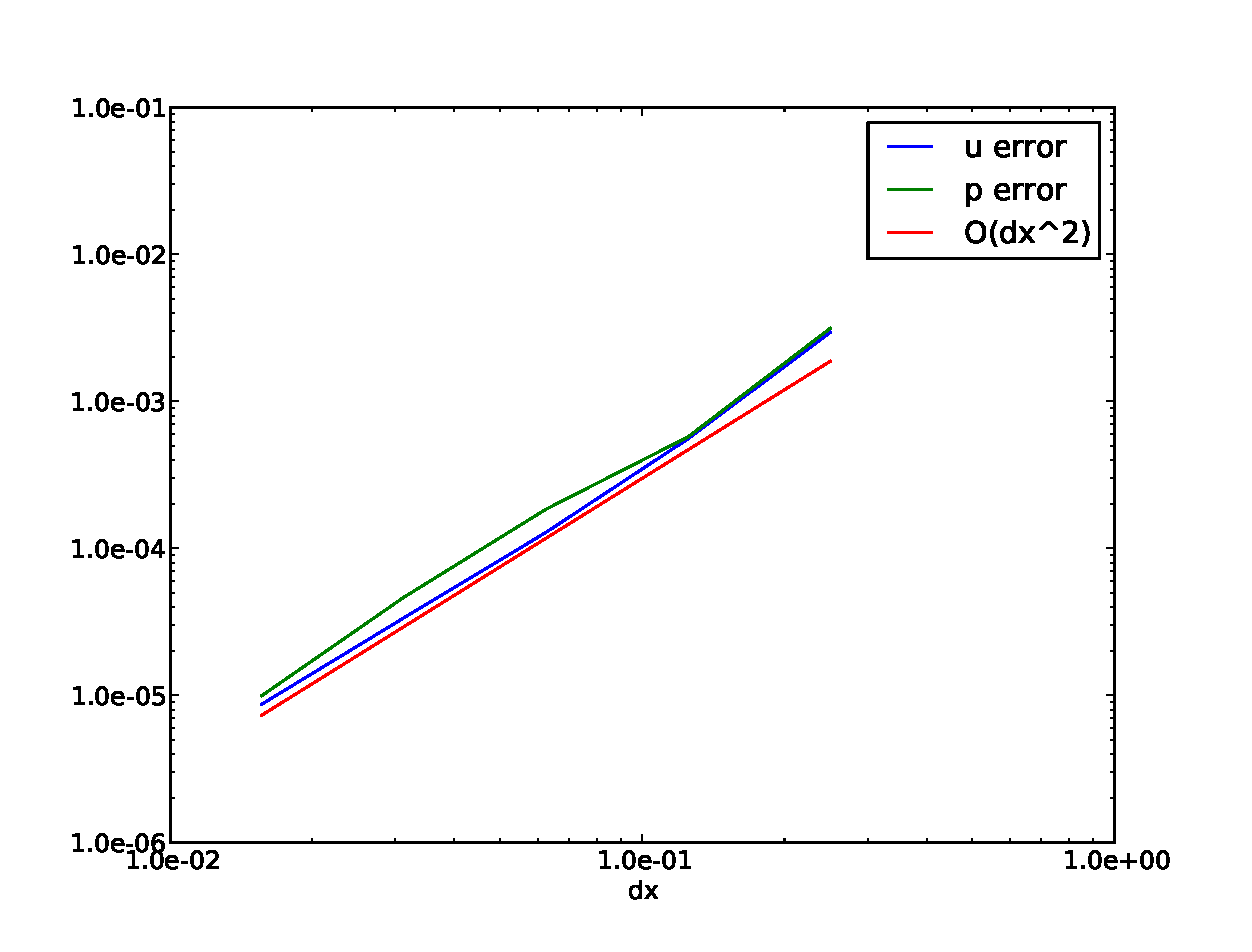
\includegraphics[width=1.1\textwidth]{examples_images/rotating_channel/convergence.eps}
  \onlypdf{\end{pdfdisplay}}  
  \caption{Error in the pressure and velocity solutions for the rotating channel as a function of resolution.}
  \label{fig:periodic_channel_error}
\end{figure}

\subsubsection{Exercises}

This example can be used to understand the use of analytic forcing
functions in \fluidity. Try modifying the function
\lstinline[language=python]{channel_tools.forcing}. The forcing function
and the analytic velocity and pressure results can be visualised by running
the \lstinline[language=python]{plot_theory}\ script. 

Examine the rest of the \lstinline[language=python]{channel_tools}\ Python
module to see how the analytic solution is automatically calculated from the
forcing function. Next, examine the \option{AnalyticUVelocitySolutionError}\
and \option{AnalyticPressureSolutionError} to see how this is used to
calculate the error in the model solution. The documentation of the Python
state interface in appendix \ref{chap:python}\ may be useful.

% %%%%%%%%%%%%%%%%%%%%%%%%%%%%%%%%%%%%%%%%%%%%%%%%%%%%%%%%%%%%%%%%%%%
% %---Open ocean deep convection--------------------%
% %%%%%%%%%%%%%%%%%%%%%%%%%%%%%%%%%%%%%%%%%%%%%%%%%%%%%%%%%%%%%%%%%%%
% 
% \section{Open ocean deep convection}
% \label{sect:OODC}
% \subsection{Overview}
% Open-ocean deep convection (OODC) has been recognised as an
% important mixing process for over 25 years, and
% has been studied in the ocean, simulated in the laboratory, and modelled numerically.
% A much-cited study in the field of numerically simulating
% open-ocean deep convection is that of \cite{jones1993} and this is recreated here.
% In their work, a fixed resolution ($240 \times 240 \times
% 100$m in $X, Y, Z$) model is used to study the physics and
% characteristic scalings of OODC. Their simulations use a disc
% of cooling in a simple box geometry to investigate the effects of rotation.
% 
% Ocean convection is important to the meridional overturning
% circulation. It is a small scale non-hydrostatic process which
% is difficult to capture in general circulation models. Applying
% an unstructured adaptive mesh model to study this process is
% novel, and this approach may produce new insights into the
% simulation and parameterisation of convection in structures and
% unstructured mesh models.
% 
% Although OODC itself is a small-scale process, it interacts with
% processes on the basin-scale, both in the preconditioning stage and
% in the sinking and spreading stages. It is therefore important for us
% to be able to represent a large range of scales. Finite elements and adapting
% unstructured meshes are particularly suited for this application, as the
% resolution used can vary in size smoothly over a wide area.
% 
% \subsection{Configuration}
% 
% \subsubsection{Geometry}
% 
% %\begin{figure}
% %\centering
% %\pdffig[width=8.0cm]{images/oodc-schematic.pdf}
% %\caption{Schematic of the domain for the three-dimensional open ocean deep convection
% %problem.}
% %\label{Fig:Schematic}
% %\end{figure}
% 
% 
% A schematic of the domain is shown in figure \ref{Fig:Schematic}.
% The domain is 32km square in the horizontal and 2km deep. A cooling disk of radius
% 8km is centred at middle of the upper boundary.
% 
% 
% 
% 
% \subsubsection{Parameters}
% The thermal expansion coefficient is set to
% $\alpha=2 \times 10^{-4} \,\mathrm{K}^{-1}$ and gravity to $g=9.81 \,\mathrm{m}\,\mathrm{s}^{-2}$.
% 
% The eddy viscosity
% and thermal diffusivity were set to the same values as those
% used in \cite{jones1993}: $\kappa_h = 5.0 \mathrm{m}^2\mathrm{s}^{-1}$ and
% $\kappa_v = 0.2 \mathrm{m}^2\mathrm{s}^{-1}$.
% 
% 
% \subsubsection{Initial and boundary conditions}
% The domain is initialised at rest with a weak temperature stratification
% in the vertical, with a top-to-bottom temperature difference of
% $0.05\,$K.
% This therefore corresponds to a buoyancy frequency ($N$) value
% of $2.2 \times 10^{-4} \,\mathrm{s}^{-1}$.
% 
% 
% A heat loss of $-800\,\mathrm{W}\,\mathrm{m}^{-2}$ is
% applied as a flux boundary condition. Assuming density $\rho=1000\,\mathrm{Kg}\,\mathrm{m}^{-3}$,
% specific heat capacity $c_p=4\times 10^3\,\mathrm{J}\,\mathrm{Kg}^{-1}\,\mathrm{K}^{-1}$,
% the flux $q=\bmn\cdot\left ( \kaptens_T  \nabla T\right)$
% takes the value $q = 2\times 10^{-4}\,\mathrm{K}\,\mathrm{m}^{-1}\,\mathrm{s}^{-1}$.
% This value is applied in a disk of radius $7750\,\mathrm{m}$ with a linear ramp to zero flux to a radius
% $8000\,\mathrm{m}$. In addition, this forcing is only applied for the first 48 hours of the simulation and
% then switched off, so that the restratification stage of the problem can be considered.
% 
% 
% 
% No-normal flow, free-stress boundary conditions are applied at the upper and lateral
% (spanwise) boundaries.
% 
% 
% \subsection{Results}
% 
% 
% 

\section{Water column collapse}
\label{sect:water_collapse}

\subsection{Overview}
A commonly used validation experiment for multi-material models is that of a collapsing column of liquid, normally water, within an atmosphere or vacuum \citep{lakehal_interface_2002}, also known as the dam break problem.  In the experimental set-up a reservoir of water is held behind an impermeable barrier separating it from the rest of the tank.  The barrier is then quickly removed, allowing the water column to collapse and flood the remaining sections of the tank.  In the numerical analogue the initial condition is generally taken as the trapped water column, still behind the dam.  At the start of the simulation the barrier is imagined to have been removed instantaneously and switching on gravity, $|g| = 9.81$, causes the column to collapse.   Several experimental set-ups have been published and used as comparison and validation tools for numerical models \citep{martin_part_1952, greaves_simulation_2006}.  Those with water depth gauges distributed throughout the tank are particularly useful, allowing the direct comparison of data.  Furthermore, pressure gauges located on the tank walls or on any obstacles within the tank provide another useful validation tool.

In this example, \fluidity\ is used to simulate a simple dam break experiment \citep{zhou_nonlinear_1999}.  The example demonstrates the following functionality:

\begin{itemize}
\item 2D flow
\item Multi-material flow
\item Incompressible flow
\item Inviscid flow
\item Mesh adaptivity
\item Static detectors
\end{itemize}

The simulation illustrated here took $\sim$2 hours to run in serial on a Intel Xeon X5355 2.66 GHz processor.

\subsection{Problem specification}
The experiment on which this example is based was a simple dam break problem in a $3.22\times2\times1m$ (length $\times$ height $\times$ depth) tank \citep{zhou_nonlinear_1999}.  A reservoir of water $1.2\times0.6\times1m$ (length $\times$ height $\times$ depth) was held behind a barrier at one end of the tank.  Water depth gauges were placed at two points, marked H1 and H2 in Figure \ref{fig:zhouinitial}(a), at $x_1 = 2.725m$ and $2.228m$ respectively.  Additionally, a pressure gauge was located at the point marked P2 in Figure \ref{fig:zhouinitial}(a), at $x_2=0.16m$ on the wall facing the initial water column.

As no variations were introduced in the third dimension, the experiment is reproduced here numerically in two dimensions within the domain $\Omega$: $x_1 \in [0,3.22]$, $x_2 \in [0,2]$ \citep{lee_numerical_2002, colagrossi_numerical_2003, park_volume-of-fluid_2009}.  The two materials (water and air) are distinguished by scalar fields $\alpha_k$ representing their volume fraction, where the volume fraction of air $\alpha_2 = 1-\alpha_1$ and $\alpha_1$ is the volume fraction of water. The initial condition of the water volume fraction is shown in Figure \ref{fig:zhouinitial}(a).  The presence of water is indicated as a grey region and the interface to air is delineated by contours at volume fraction values of $0.025$, $0.5$ and $0.975$.  The densities of the water and air are taken as $ 1,000kg\,m^{-2}$ and $1kg\,m^{-2}$ respectively.  Both fluids are treated inviscidly. As the simulation is inviscid, free slip boundary conditions are imposed on the tank bottom, $x_2=0$, and sides, $x_1=0,\,3.22$.  The top of the tank, $x_2=2$, is left open.

\begin{figure}[tbp]
\hspace{1cm}(a)
\begin{center}
% modified from initial_setup.pdf_t, which was generated by xfig from initial_setup.fig
% modifications are a simple rescaling to 0.71 of original size
\begin{picture}(0,0)%
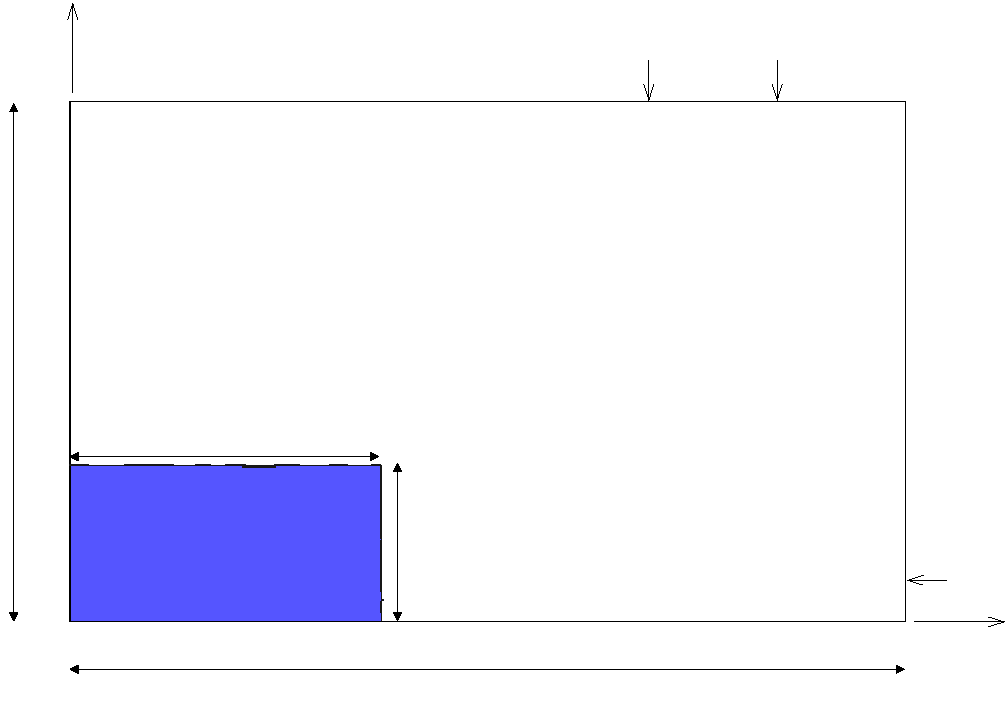
\includegraphics[scale=0.71]{examples_images/water_collapse/initial_setup.pdf}%
\end{picture}%
\setlength{\unitlength}{2942.24sp}%
%
\begingroup\makeatletter\ifx\SetFigFont\undefined%
\gdef\SetFigFont#1#2#3#4#5{%
  \reset@font\fontsize{#1}{#2pt}%
  \fontfamily{#3}\fontseries{#4}\fontshape{#5}%
  \selectfont}%
\fi\endgroup%
\begin{picture}(7677,5377)(2101,-9251)
\put(5761,-5326){\makebox(0,0)[lb]{\smash{{\SetFigFont{10}{12.0}{\familydefault}{\mddefault}{\updefault}{\color[rgb]{0,0,0}Air}%
}}}}
\put(2746,-4021){\makebox(0,0)[lb]{\smash{{\SetFigFont{10}{12.0}{\familydefault}{\mddefault}{\updefault}{\color[rgb]{0,0,0}$x_2$}%
}}}}
\put(5356,-4561){\makebox(0,0)[lb]{\smash{{\SetFigFont{10}{12.0}{\familydefault}{\mddefault}{\updefault}{\color[rgb]{0,0,0}$p = 0$}%
}}}}
\put(7111,-4246){\makebox(0,0)[b]{\smash{{\SetFigFont{10}{12.0}{\familydefault}{\mddefault}{\updefault}{\color[rgb]{0,0,0}2.228$m$}%
}}}}
\put(8101,-4246){\makebox(0,0)[b]{\smash{{\SetFigFont{10}{12.0}{\familydefault}{\mddefault}{\updefault}{\color[rgb]{0,0,0}2.725$m$}%
}}}}
\put(7066,-4021){\makebox(0,0)[b]{\smash{{\SetFigFont{10}{12.0}{\familydefault}{\mddefault}{\updefault}{\color[rgb]{0,0,0}H2}%
}}}}
\put(8056,-4021){\makebox(0,0)[b]{\smash{{\SetFigFont{10}{12.0}{\familydefault}{\mddefault}{\updefault}{\color[rgb]{0,0,0}H1}%
}}}}
\put(9586,-8881){\makebox(0,0)[lb]{\smash{{\SetFigFont{10}{12.0}{\familydefault}{\mddefault}{\updefault}{\color[rgb]{0,0,0}$x_1$}%
}}}}
\put(9676,-8341){\makebox(0,0)[b]{\smash{{\SetFigFont{10}{12.0}{\familydefault}{\mddefault}{\updefault}{\color[rgb]{0,0,0}0.16$m$}%
}}}}
\put(9676,-8116){\makebox(0,0)[b]{\smash{{\SetFigFont{10}{12.0}{\familydefault}{\mddefault}{\updefault}{\color[rgb]{0,0,0}P2}%
}}}}
\put(5761,-9196){\makebox(0,0)[b]{\smash{{\SetFigFont{10}{12.0}{\familydefault}{\mddefault}{\updefault}{\color[rgb]{0,0,0}3.22$m$}%
}}}}
\put(2116,-6631){\makebox(0,0)[rb]{\smash{{\SetFigFont{10}{12.0}{\familydefault}{\mddefault}{\updefault}{\color[rgb]{0,0,0}2.0$m$}%
}}}}
\put(4051,-7261){\makebox(0,0)[rb]{\smash{{\SetFigFont{10}{12.0}{\familydefault}{\mddefault}{\updefault}{\color[rgb]{0,0,0}1.2$m$}%
}}}}
\put(5446,-8071){\makebox(0,0)[b]{\smash{{\SetFigFont{10}{12.0}{\familydefault}{\mddefault}{\updefault}{\color[rgb]{0,0,0}0.6$m$}%
}}}}
\put(3601,-7036){\makebox(0,0)[lb]{\smash{{\SetFigFont{10}{12.0}{\familydefault}{\mddefault}{\updefault}{\color[rgb]{0,0,0}Water}%
}}}}
\put(5896,-8836){\makebox(0,0)[b]{\smash{{\SetFigFont{10}{12.0}{\familydefault}{\mddefault}{\updefault}{\color[rgb]{0,0,0}$u_in_i = 0$}%
}}}}
\put(2476,-6586){\rotatebox{90.0}{\makebox(0,0)[b]{\smash{{\SetFigFont{10}{12.0}{\familydefault}{\mddefault}{\updefault}{\color[rgb]{0,0,0}$u_in_i = 0$}%
}}}}}
\put(9136,-6586){\rotatebox{270.0}{\makebox(0,0)[b]{\smash{{\SetFigFont{10}{12.0}{\familydefault}{\mddefault}{\updefault}{\color[rgb]{0,0,0}$u_in_i = 0$}%
}}}}}
\end{picture}%

\end{center}
\hspace{1cm}(b)
\begin{center}
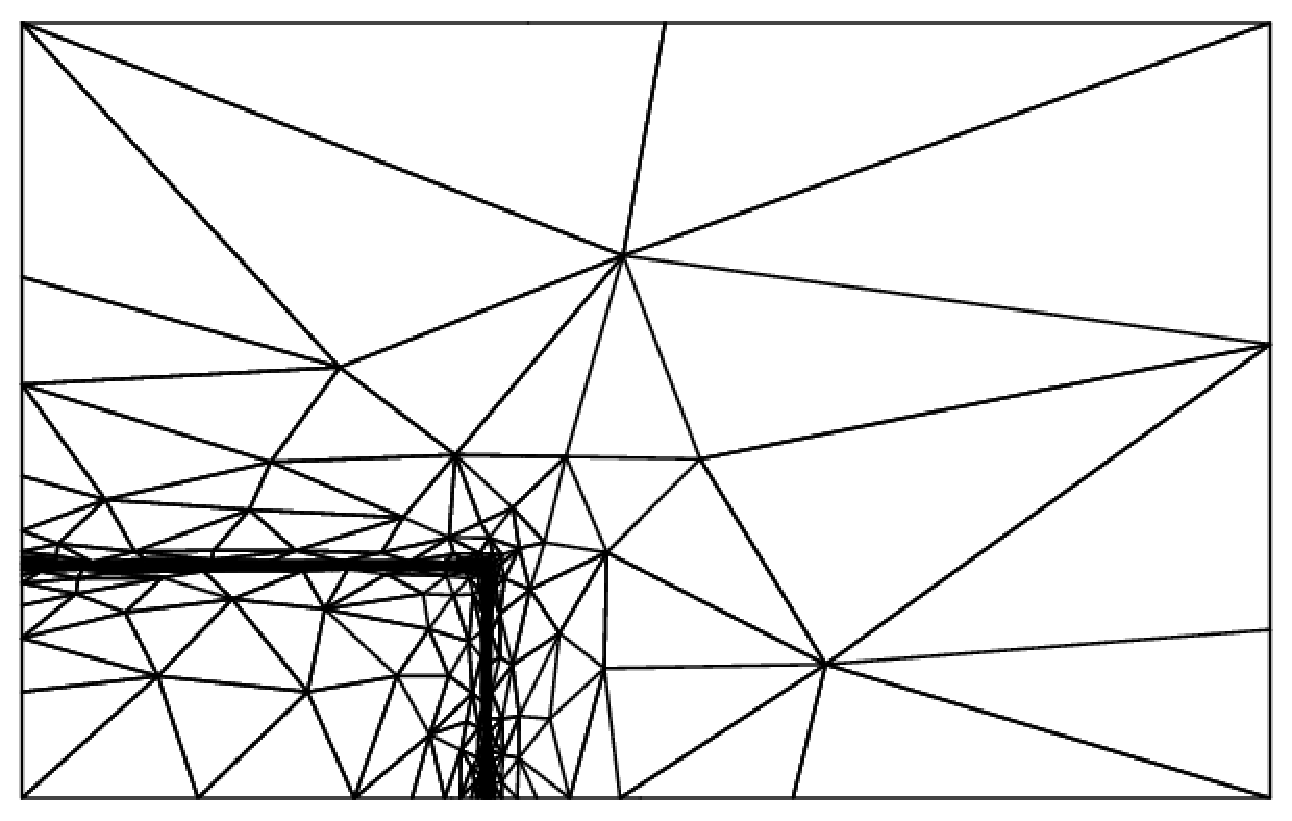
\includegraphics[width=10.2cm, trim=2.5cm 4.5cm 2.5cm 4.5cm, clip=true]{examples_images/water_collapse/water_collapse_0_mesh.pdf}
\end{center}
\caption{(a) Initial set-up of the water volume fraction, $\alpha_1$, and the velocity and pressure boundary conditions for the two-dimensional water column collapse validation problem \citep{zhou_nonlinear_1999}. The presence of water is indicated as a grey region and the interface to air is delineated by contours of the volume fraction at $0.025$, $0.5$ and $0.975$.  The locations of the pressure (P2) and water depth gauges (H1, H2) are also indicated. (b) The adapted mesh used to represent the initial conditions.}
\label{fig:zhouinitial}
\end{figure}

The water volume fraction, $\alpha_1$, is solved for using an advection equation (REFMARKER).  It is advected using HyperC on a control volume mesh (REFMARKER), while the velocity and pressure are discretised using the P0P1$_{\text{CV}}$ element pair (REFMARKER) with $\theta=1/2$ and $\theta_i=1/2$ (REFMARKER).  

This example employs an adaptive mesh (REFMARKER). The minimum edge length in the mesh is constrained to $2mm$. The upper bound on the edge lengths was specified as half the domain length and height in each dimension.  The pressure and water volume fraction were directly adapted to using interpolation error bounds, $\hat{\epsilon}$, of $1,000$ and $0.05$ respectively.  As the velocity is element centred it was first projected to the vertices before being adapted to with an interpolation error bound of $1$ for each component.  Given the ranges of these fields seen in the fixed mesh runs these correspond to desired errors of less than 5\% for each field. The volume fraction is transferred between successive meshes using a minimally diffusive bounded projection algorithm.  The velocity is transferred using a straightforward projection while the pressure is consistently interpolated using the linear basis functions from its parent mesh. For details of the remaining adaptivity settings we refer to the documented flml file.  The initial mesh using these settings is shown in Figure \ref{fig:zhouinitial}(b). 

The timestep is selected to achieve a Courant number (REFMARKER) of $2.5$ while the advection equation uses approximately $10$ subcycles (REFMARKER) so the volume fraction is advected at a Courant number of $0.25$.  

\subsection{Results}
Several timesteps of the example simulation can be seen in Figure \ref{fig:zhouwholea} where the interface is represented by contours of the water volume fraction, $\alpha_1$, at $0.025$, $0.5$ and $0.975$.  Similar images can be generated by visualising the vtu files using Paraview or Mayavi2 (REFMARKER).

\begin{figure}[tbp]
\begin{center}
% \newcolumntype{V}{>{\centering\arraybackslash} m{7cm} }
\begin{tabular}{ll}
(a) $t = 0.5$ & (b) $t = 1.0$   \\
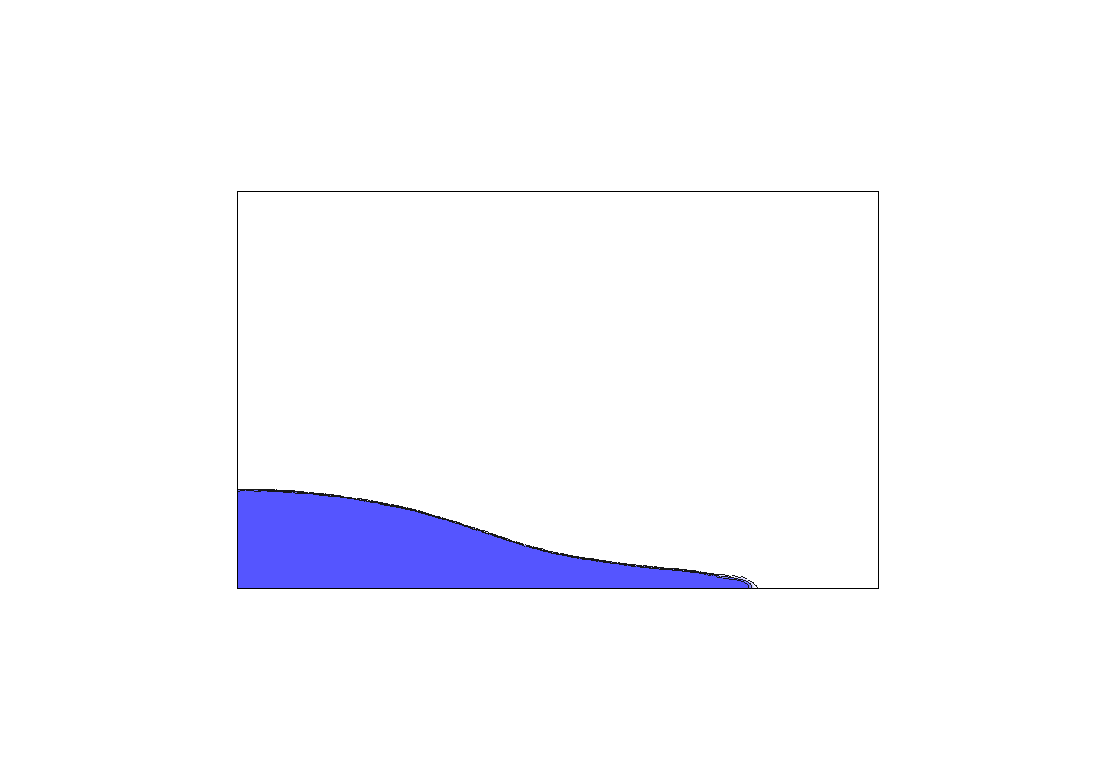
\includegraphics[width=7cm, trim=2.5cm 4.5cm 2.5cm 4.5cm, clip=true]{examples_images/water_collapse/water_collapse_100.png} & 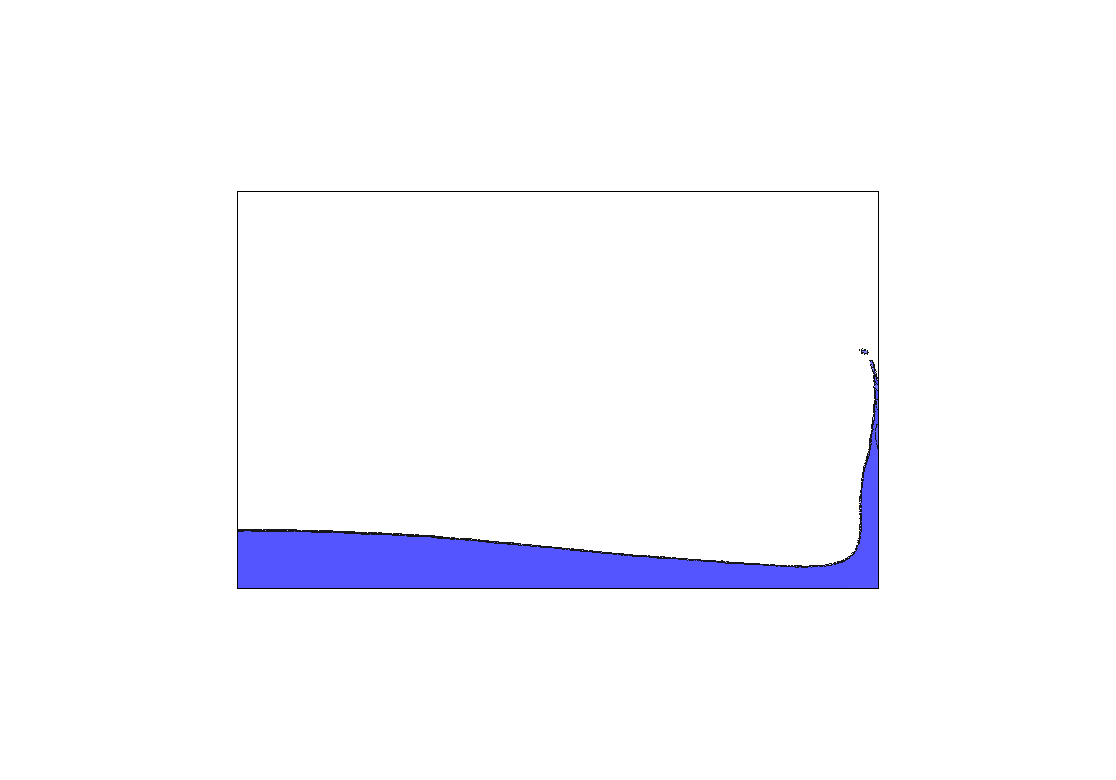
\includegraphics[width=7cm, trim=2.5cm 4.5cm 2.5cm 4.5cm, clip=true]{examples_images/water_collapse/water_collapse_200.png} \\
(c) $t = 1.5$ & (d) $t = 1.625$ \\
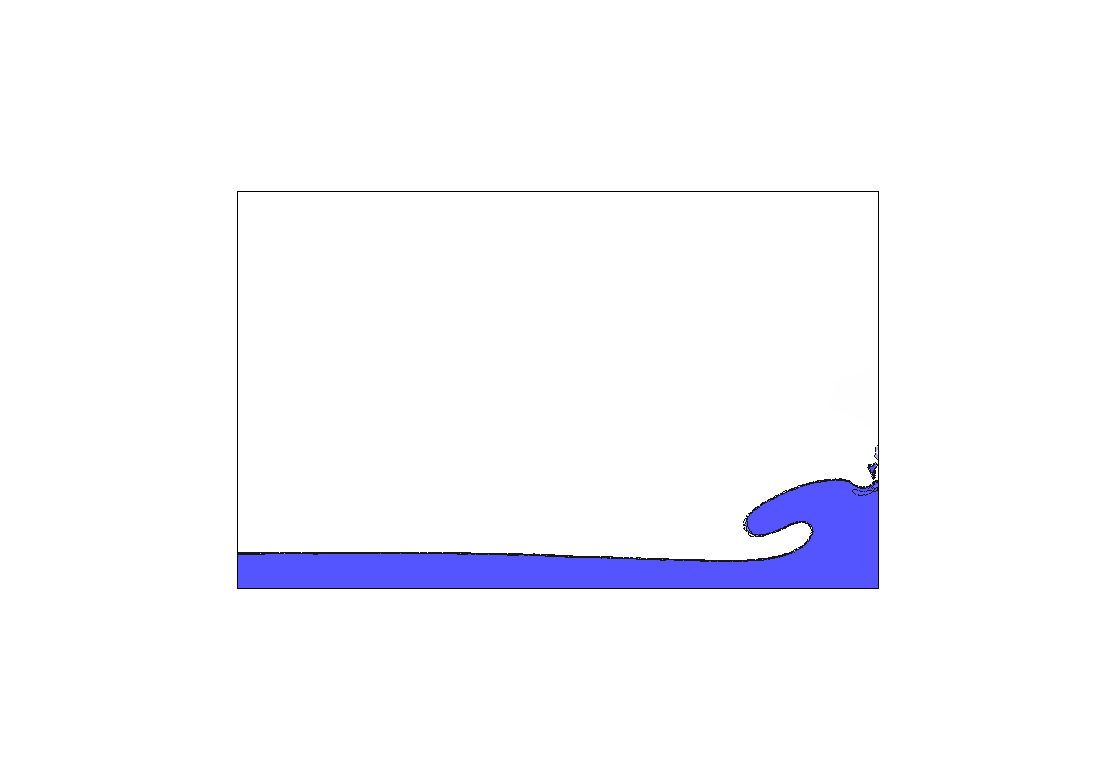
\includegraphics[width=7cm, trim=2.5cm 4.5cm 2.5cm 4.5cm, clip=true]{examples_images/water_collapse/water_collapse_300.png} & \includegraphics[width=7cm, trim=2.5cm 4.5cm 2.5cm 4.5cm, clip=true]{examples_images/water_collapse/water_collapse_325.png} \\
(e) $t = 1.75$ & (f) $t = 1.875$ \\
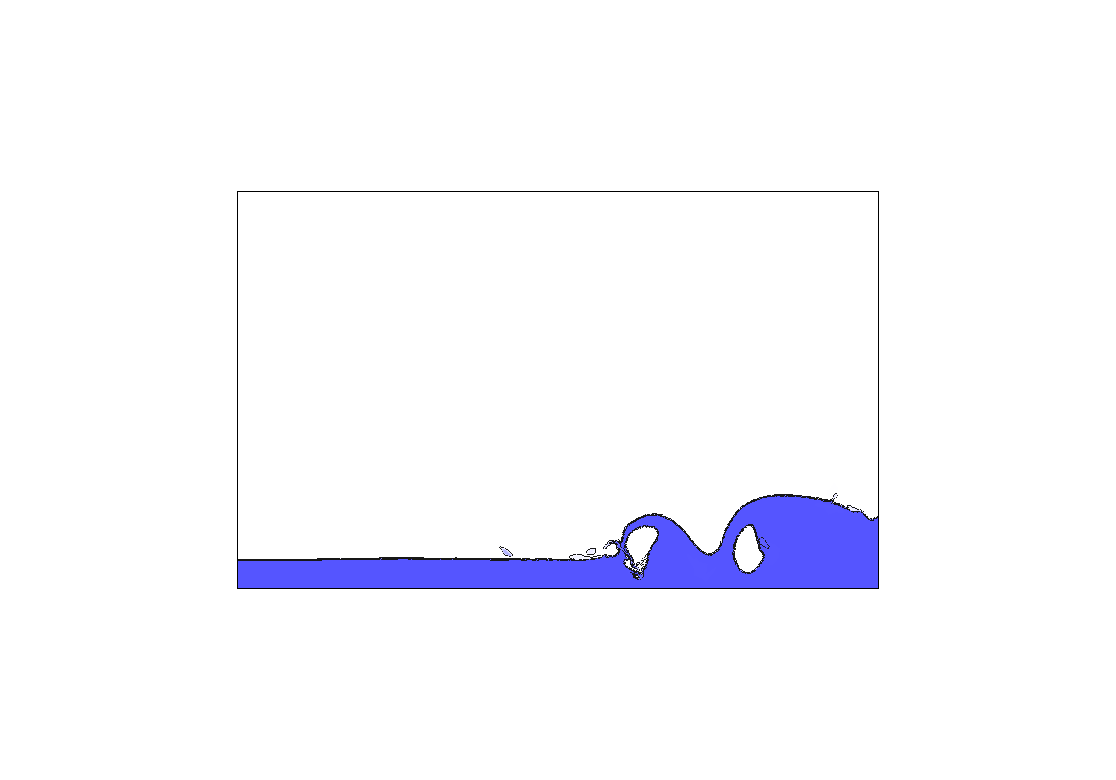
\includegraphics[width=7cm, trim=2.5cm 4.5cm 2.5cm 4.5cm, clip=true]{examples_images/water_collapse/water_collapse_350.png} & \includegraphics[width=7cm, trim=2.5cm 4.5cm 2.5cm 4.5cm, clip=true]{examples_images/water_collapse/water_collapse_375.png} \\
(g) $t = 2.0$ & (h) $t = 2.5$ \\
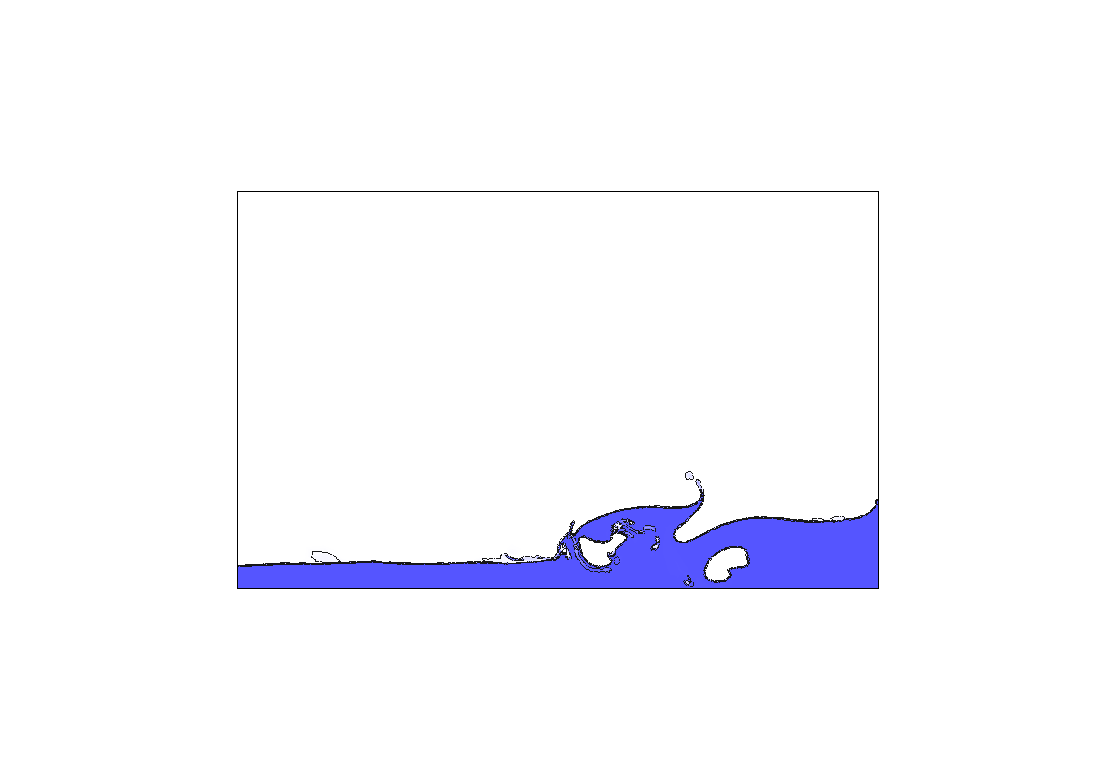
\includegraphics[width=7cm, trim=2.5cm 4.5cm 2.5cm 4.5cm, clip=true]{examples_images/water_collapse/water_collapse_400.png} & 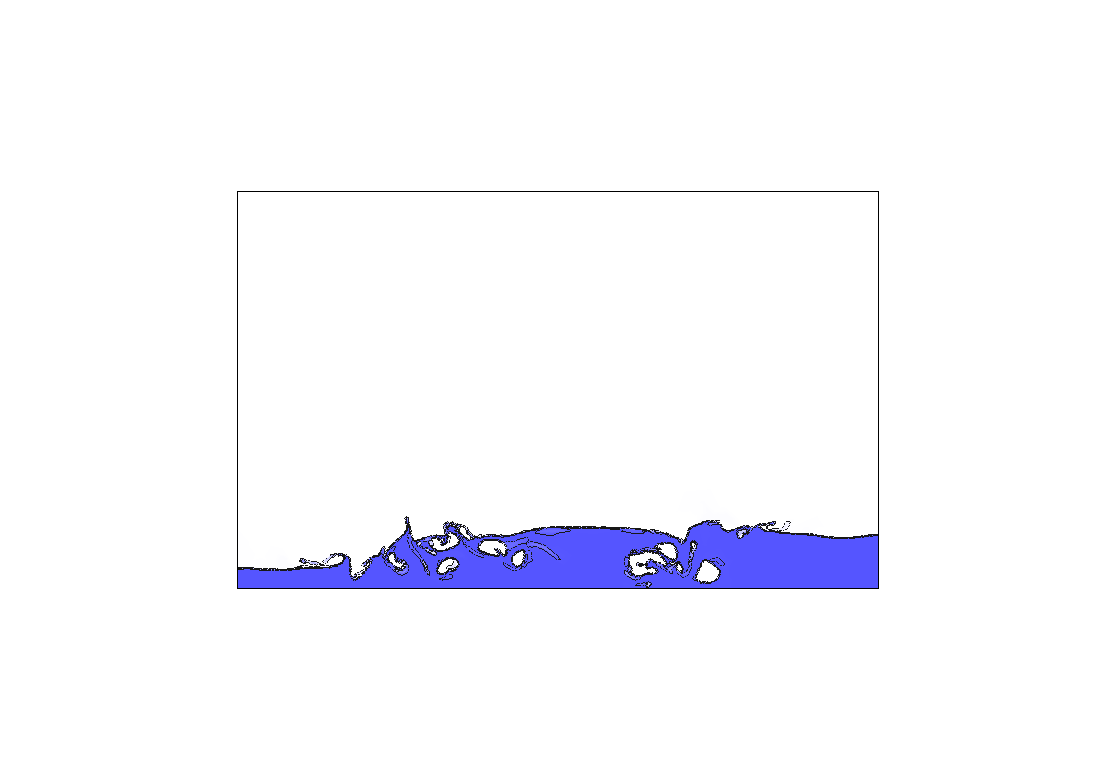
\includegraphics[width=7cm, trim=2.5cm 4.5cm 2.5cm 4.5cm, clip=true]{examples_images/water_collapse/water_collapse_500.png} \\
\end{tabular}
\caption{The evolution of the water volume fraction, $\alpha_1$, over several timesteps.  The presence of water, $\alpha_1=1$, is indicated as a grey region and the interface to air, $\alpha_1=0$, is delineated by contours at $\alpha_1 = 0.025$, $0.5$ and $0.975$.}
\label{fig:zhouwholea}
\end{center}
\end{figure}

\begin{figure}[tbp]
\begin{center}
% \newcolumntype{V}{>{\centering\arraybackslash} m{7cm} }
\begin{tabular}{ll}
(a) $t = 0.5$ & (b) $t = 1.0$\\
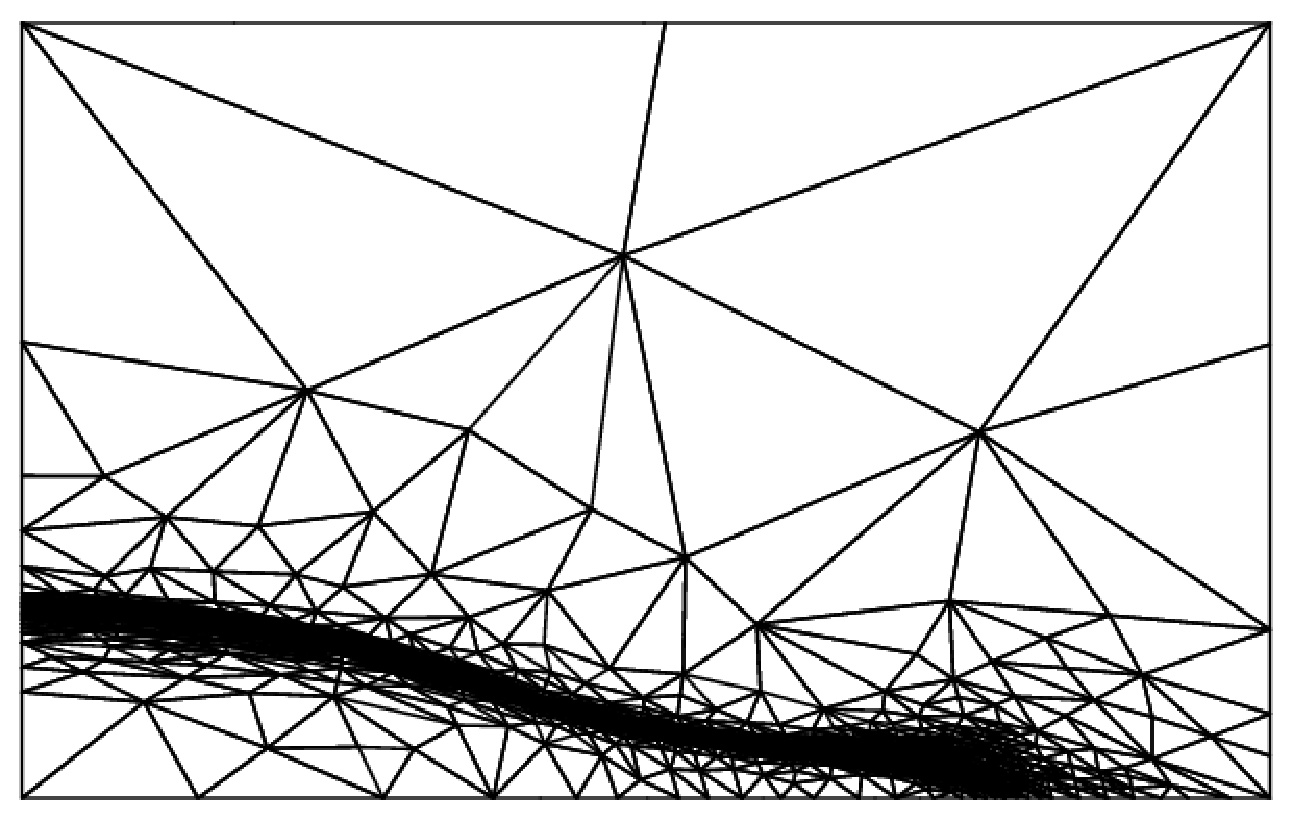
\includegraphics[width=7cm, trim=2.5cm 4.5cm 2.5cm 4.5cm, clip=true]{examples_images/water_collapse/water_collapse_100_mesh.pdf} & 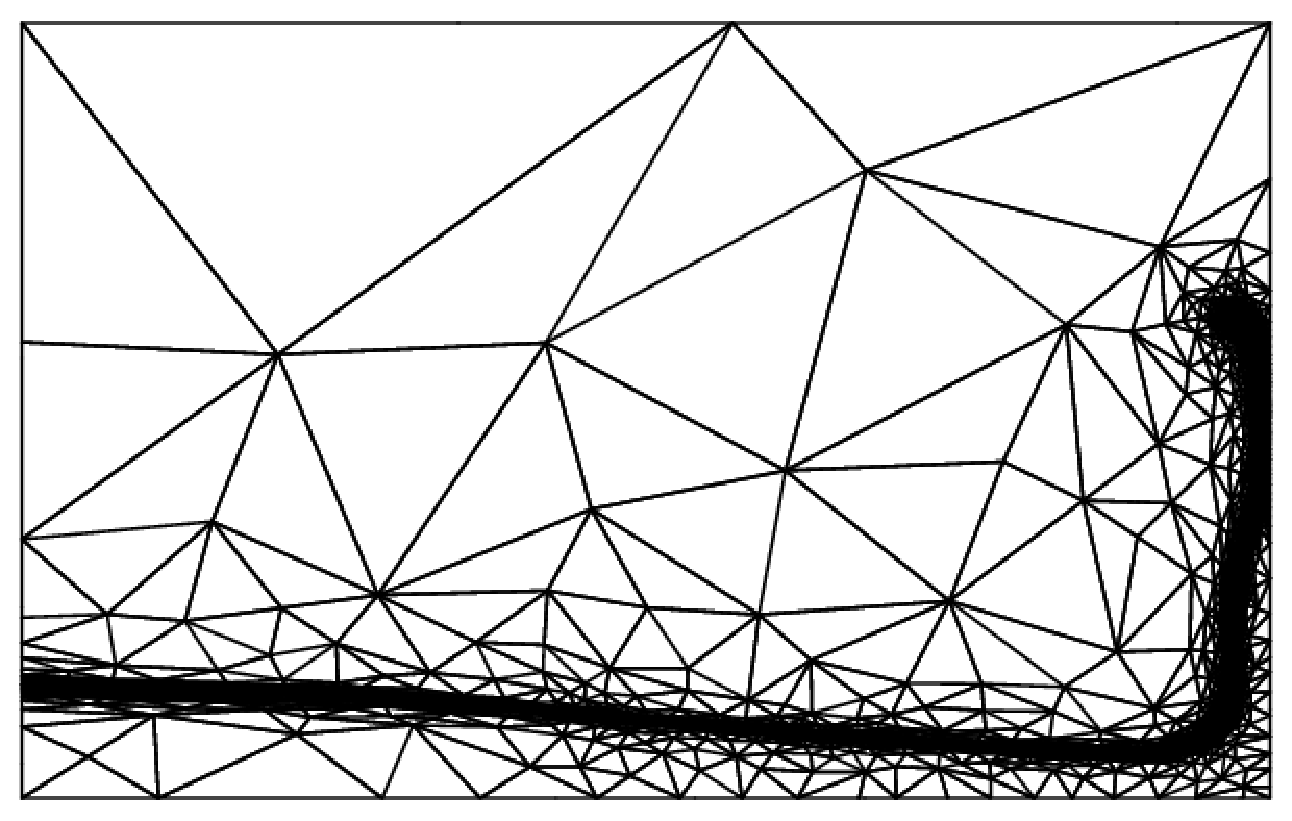
\includegraphics[width=7cm, trim=2.5cm 4.5cm 2.5cm 4.5cm, clip=true]{examples_images/water_collapse/water_collapse_200_mesh.pdf} \\
(c) $t = 1.5$ & (d) $t = 1.625$ \\
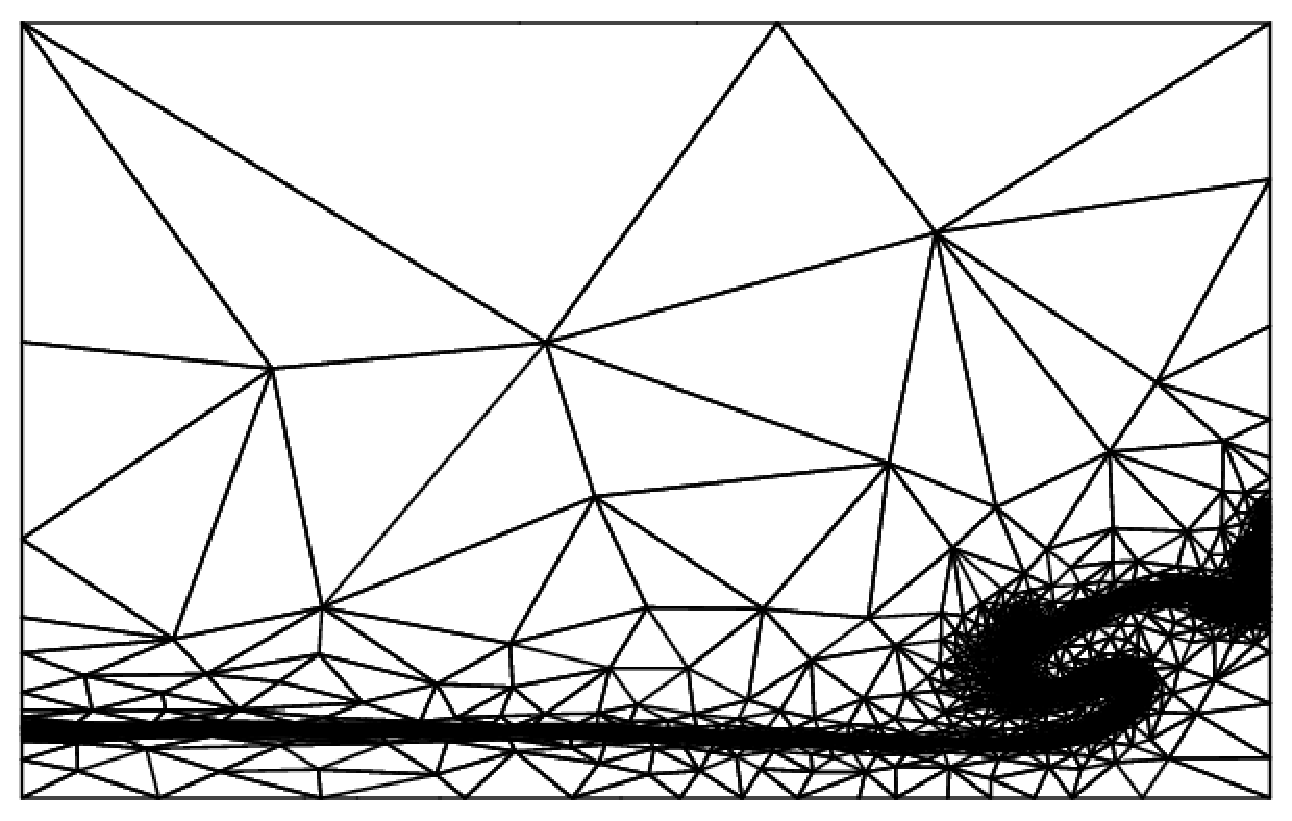
\includegraphics[width=7cm, trim=2.5cm 4.5cm 2.5cm 4.5cm, clip=true]{examples_images/water_collapse/water_collapse_300_mesh.pdf} & \includegraphics[width=7cm, trim=2.5cm 4.5cm 2.5cm 4.5cm, clip=true]{examples_images/water_collapse/water_collapse_325_mesh.pdf} \\
(e) $t = 1.75$ & (f) $t = 1.875$ \\
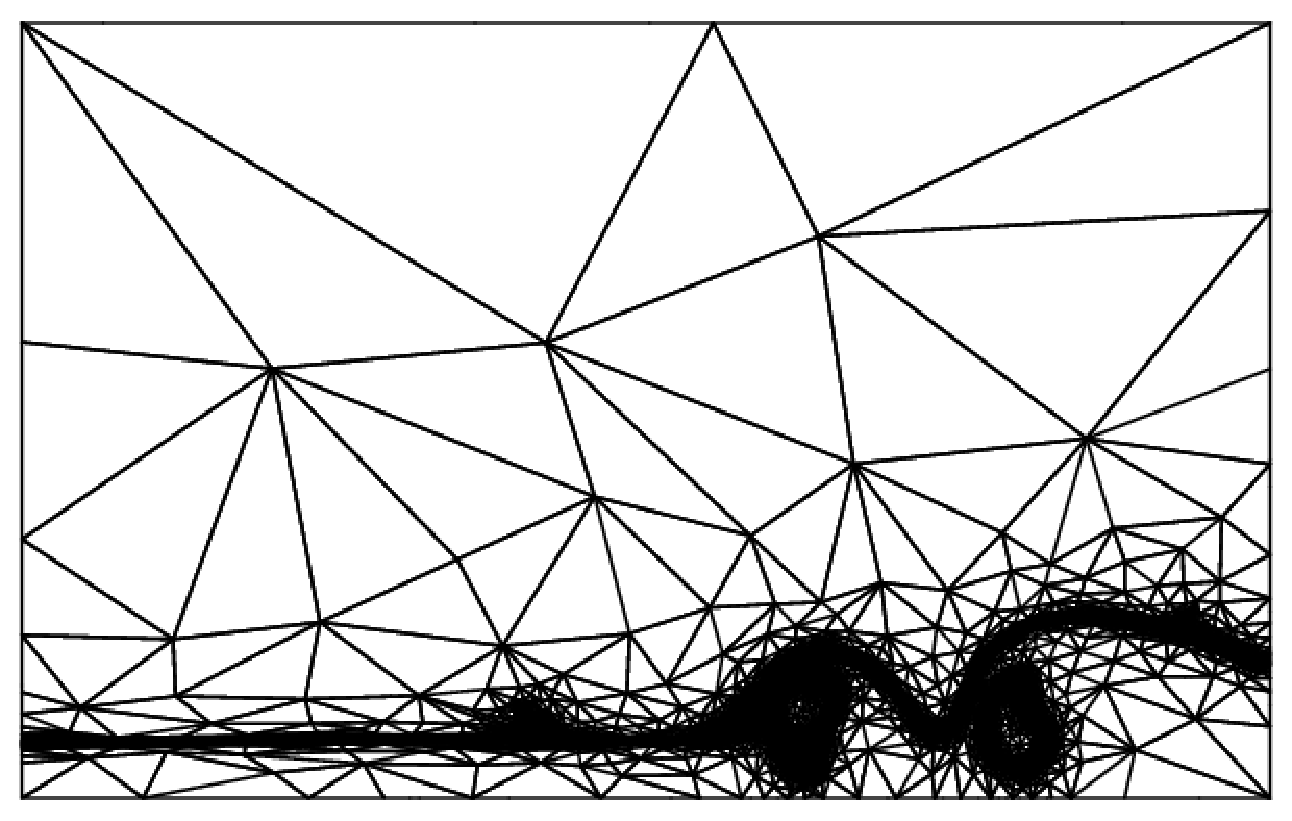
\includegraphics[width=7cm, trim=2.5cm 4.5cm 2.5cm 4.5cm, clip=true]{examples_images/water_collapse/water_collapse_350_mesh.pdf} & \includegraphics[width=7cm, trim=2.5cm 4.5cm 2.5cm 4.5cm, clip=true]{examples_images/water_collapse/water_collapse_375_mesh.pdf} \\
(g) $t = 2.0$ & (h) $t = 2.5$ \\
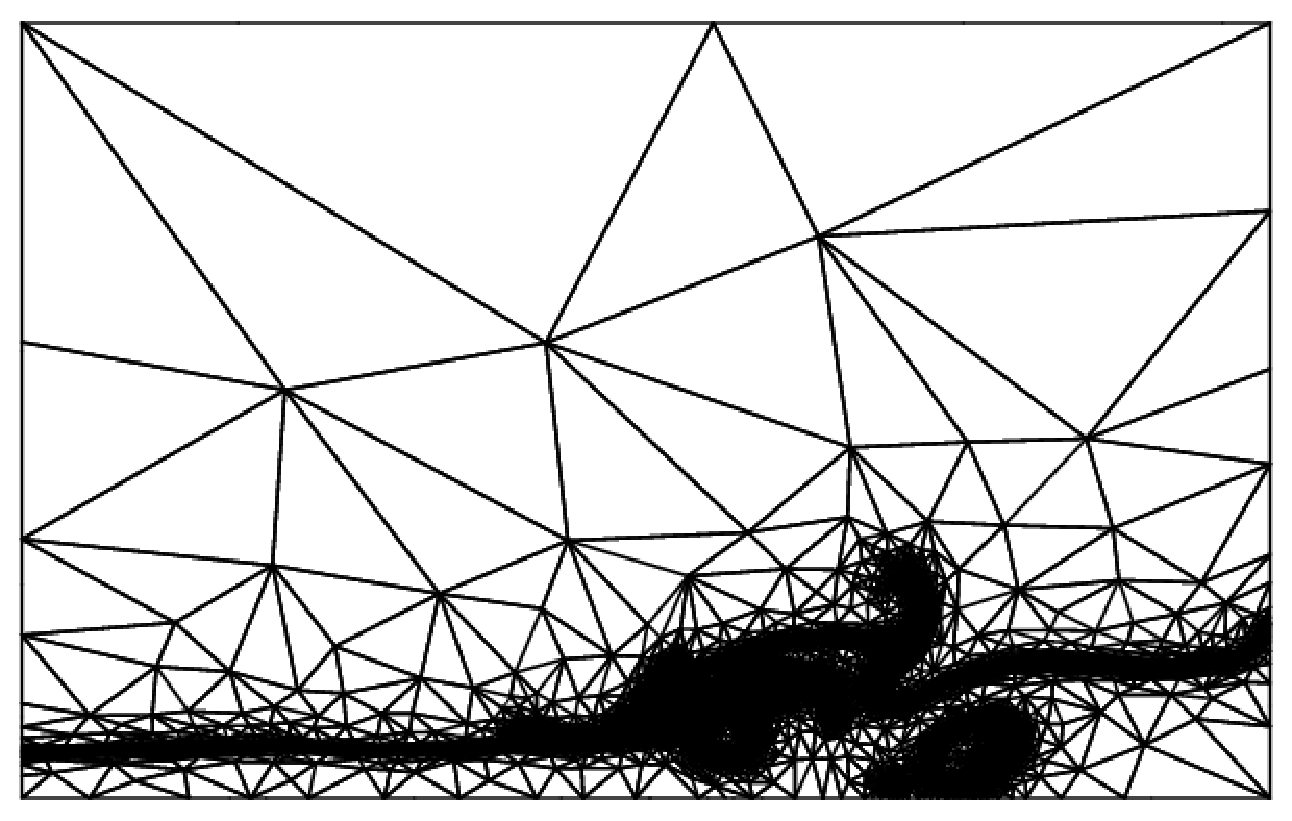
\includegraphics[width=7cm, trim=2.5cm 4.5cm 2.5cm 4.5cm, clip=true]{examples_images/water_collapse/water_collapse_400_mesh.pdf} & 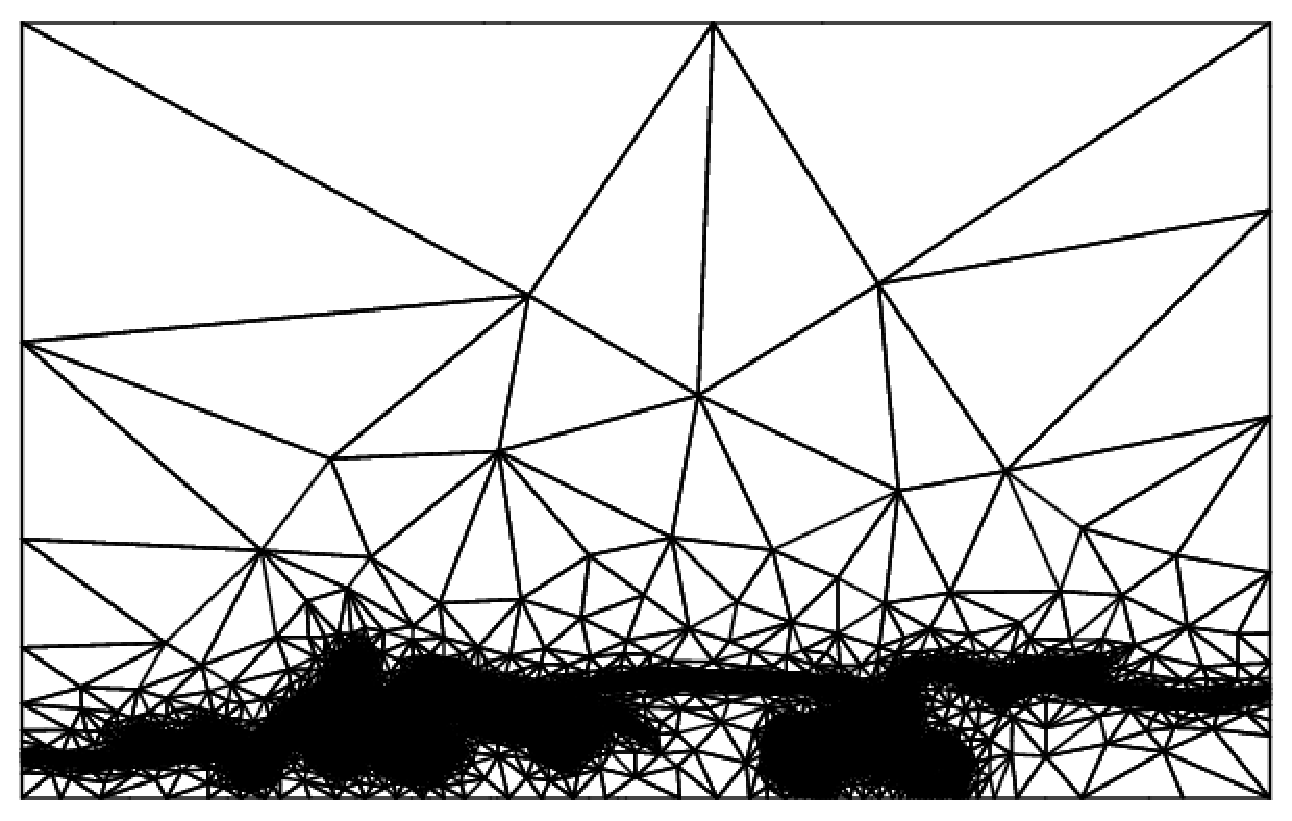
\includegraphics[width=7cm, trim=2.5cm 4.5cm 2.5cm 4.5cm, clip=true]{examples_images/water_collapse/water_collapse_500_mesh.pdf} \\
\end{tabular}
\caption{The evolution of the adaptive mesh over the same timesteps displayed in Figure \ref{fig:zhouwholea}.  The mesh can be seen to closely follow the interface between the water and air.}
\label{fig:zhouwholemesh}
\end{center}
\end{figure}

The images show the column collapse (Figure \ref{fig:zhouwholea}(a)), run-up against the opposing wall (Figure \ref{fig:zhouwholea}(b)) and the subsequent overturning wave (Figure \ref{fig:zhouwholea}(c, d)) and entrainment of air bubbles (Figure \ref{fig:zhouwholea}(e--h)).  

\begin{figure}[tbp]
\begin{center}
%\newcolumntype{V}{ m{7cm} }
\begin{tabular}{cc}
\hspace{1cm}(i) H1 & (ii) H2  \\
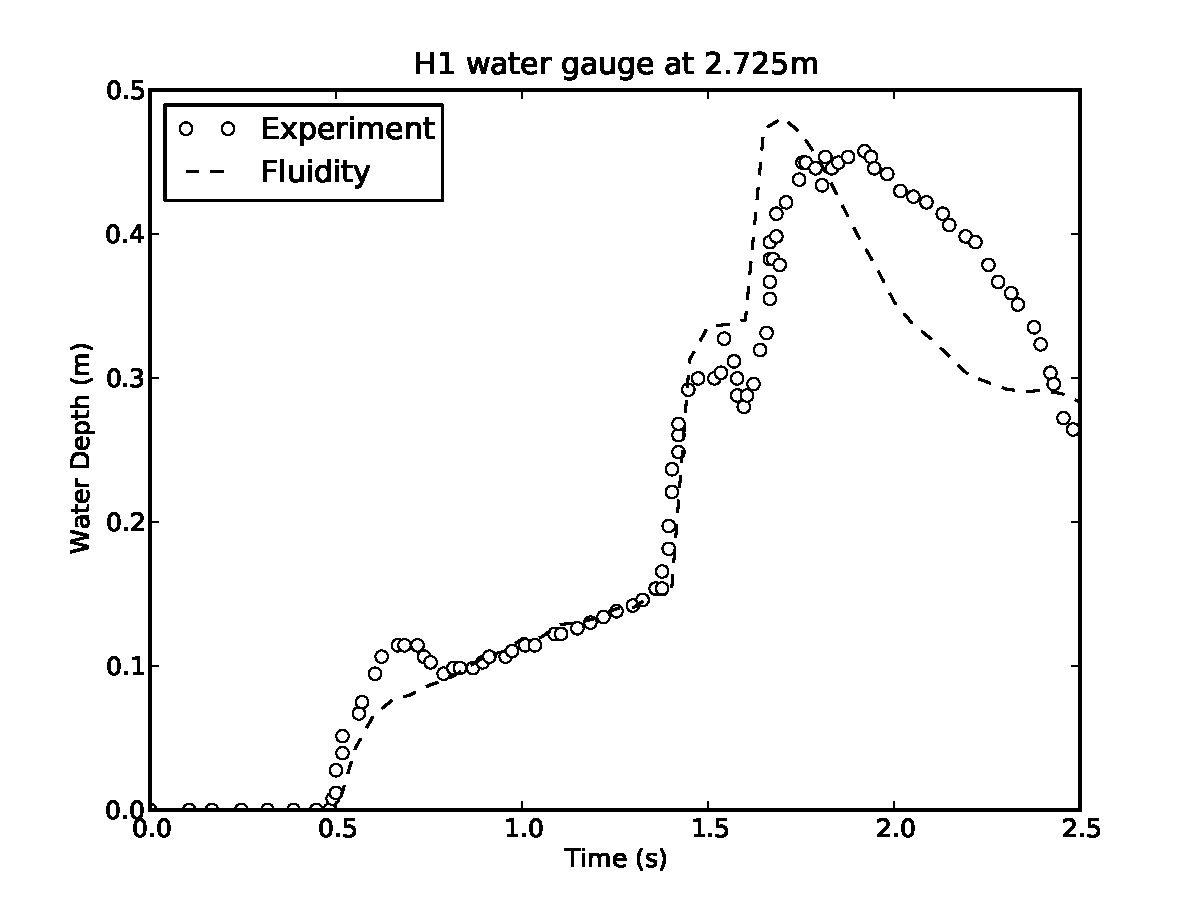
\includegraphics[width=7cm]{examples_images/water_collapse/water_gauge_H1.pdf} & 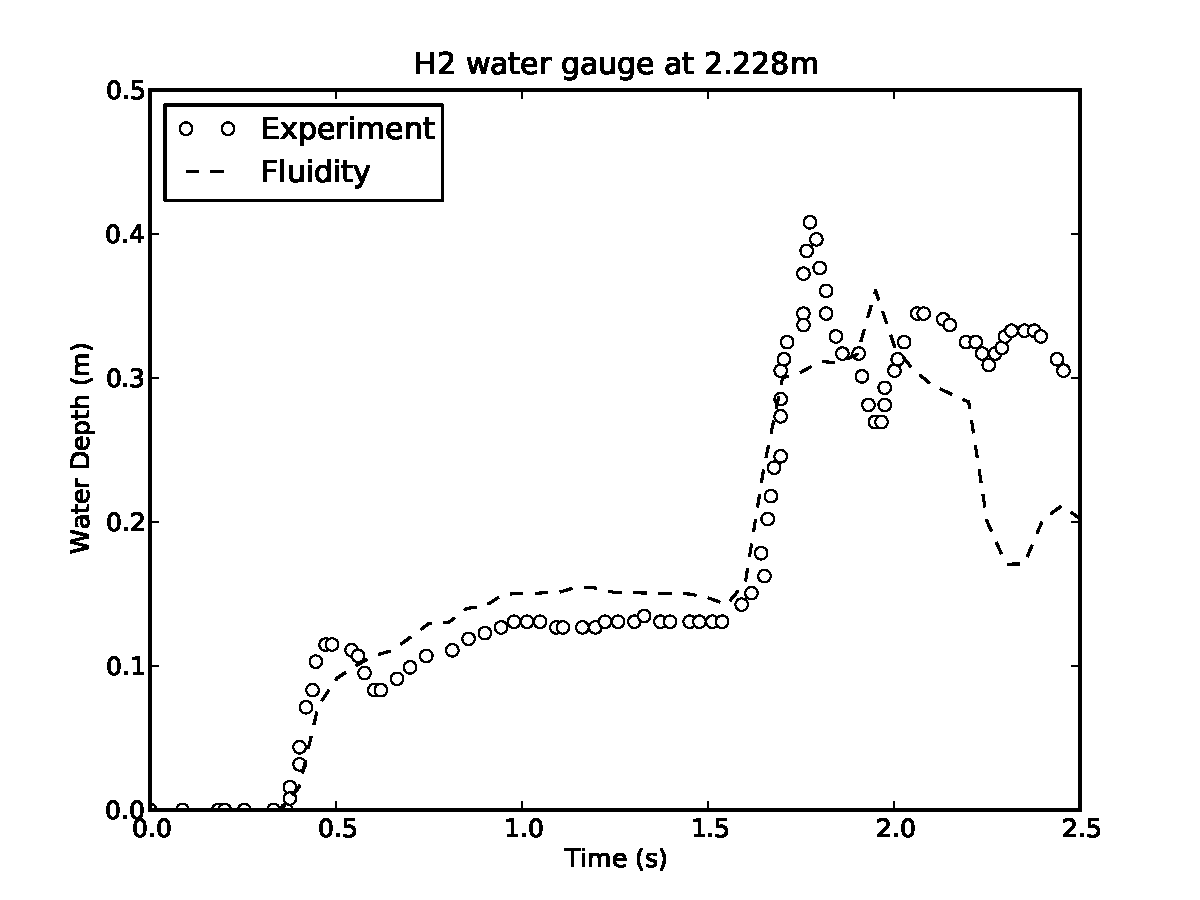
\includegraphics[width=7cm]{examples_images/water_collapse/water_gauge_H2.pdf}\\
\end{tabular}
\caption{Comparison between the experimental (circles) and numerical water gauge data at H1 (i) and H2 (ii), $x_1 = 2.725m$ and $2.228m$ respectively.  The letters along the top of the graphs indicate the times corresponding to Figure \ref{fig:zhouwholea}(a--h).  Experimental data taken from \citet{zhou_nonlinear_1999} through \citet{park_volume-of-fluid_2009}.}
\label{fig:zhoudepth}
\end{center}
\end{figure}

For validation purposes, the post-processing script provided for this example extracts information from the detector file (pressure) and from the water volume fraction field stored in the vtu files (water depth) and plots these data in comparison with the experimental results. The water depth gauge data is displayed in Figure \ref{fig:zhoudepth} alongside the experimental data.  The numerical results show the total thickness of water at the points H1 and H2, discounting any air bubbles that cross the gauges.  The simulation results show a close similarity to the experimental results with the exception of a small lip of water when the initial water head passes the gauge.  It is unclear what causes this structure, though it may be related to the initial withdrawal of the barrier in the experiment or drag effects from the bottom of the tank.  All previous published attempts to model the experiment also fail to reproduce this initial lip \citep{zhou_nonlinear_1999, lee_numerical_2002, colagrossi_numerical_2003, park_volume-of-fluid_2009}.

After $t=1.5s$ the overturning wave starts to pass the water gauges and the match between the experimental results and the numerical simulation deteriorates. As would be expected from such complex behaviour, all previous published attempts have also failed to reproduce the experimental depth gauge data after this point.  However, the broad pattern and average depth observed in the simulation after $t=1.5s$ can be seen in Figure \ref{fig:zhoudepth} to match the experiment reasonably well.

\begin{figure}[tb]
\begin{center}
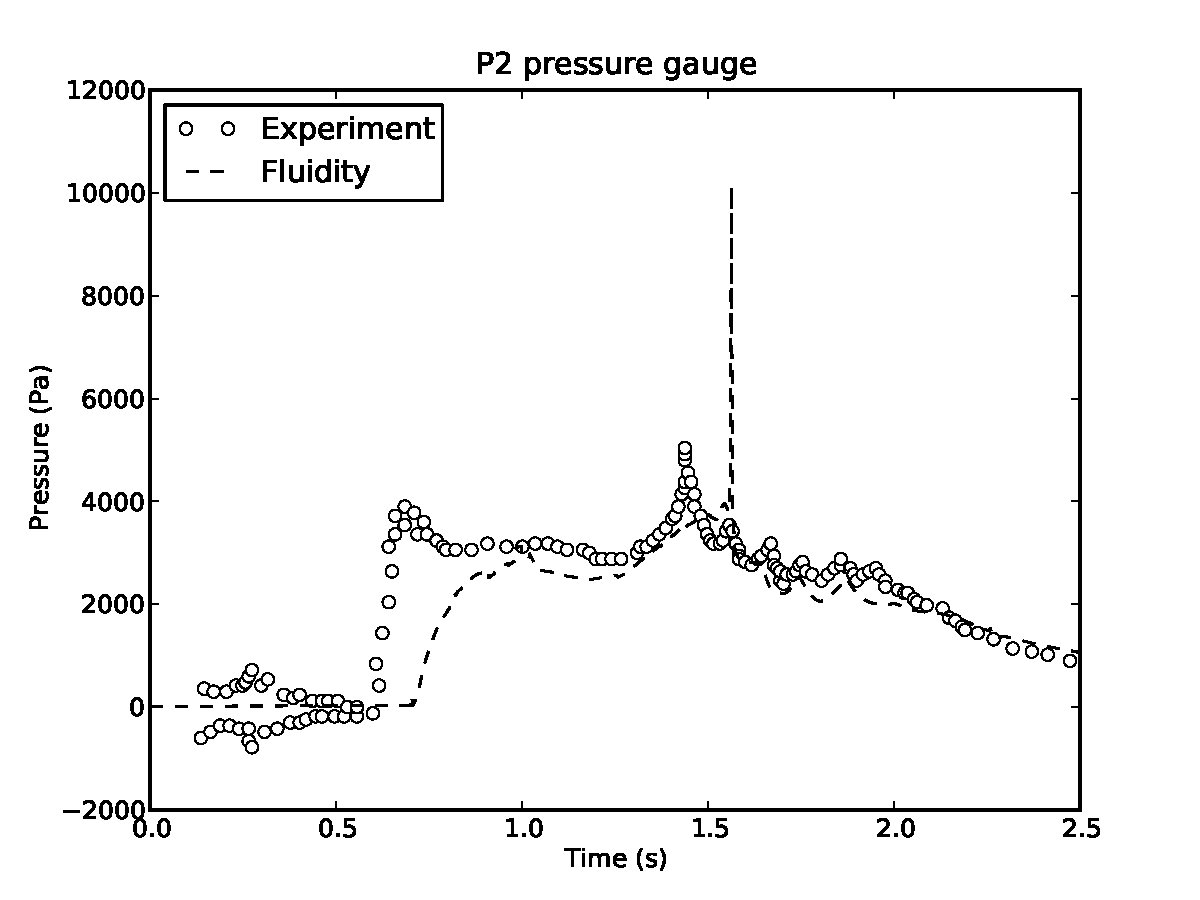
\includegraphics[width=10cm]{examples_images/water_collapse/pressure_gauge_P2.pdf}
\caption{Comparison between the experimental (circles) and numerical pressure gauge data at P2, $x_1 = 3.22m$, $x_2 = 0.16m$.  The letters along the top of the graphs indicate the times corresponding to Figure \ref{fig:zhouwholea}(a--h).  Experimental data taken from \citet{zhou_nonlinear_1999} through \citet{park_volume-of-fluid_2009}.}
\label{fig:zhoupressure}
\end{center}
\end{figure}

Experimental pressure gauge data are also available at the point P2, $(3.22,0.16)m$, on the right wall of the tank.  This is compared to the numerical pressure results in Figure \ref{fig:zhoupressure}.  After the initial noise in the experimental data, a sudden step in pressure is seen as the water run-up reaches the pressure gauge at about $t=0.6s$.  This is also seen in the numerical simulations however it is slightly delayed, occurring at $t=0.7s$.  As upwinding is being used in the discretisation of the velocity field, the delay may be due to numerical viscosity slowing the advancing water front.  However, as the delay was not as extreme at the depth gauges H1 and H2 other factors may also play a role.  For instance, if the lip seen in the experimental water gauge data is a head on the water front, that has not been reproduced numerically, it may reach the height of the pressure gauge faster than a front with no head.

Once the pressure jump occurs the experimental and numerical data are in broad agreement until the overturning wave impacts with the water layer at approximately $t=1.5s$ (Figure \ref{fig:zhouwholea}(c)).  At the point of contact a pressure pulse is transmitted to the pressure gauge resulting in a modest pressure spike in the experimental data.  This is matched by slightly delayed pressure pulses in all the numerical simulation.  However, the pulses seen in the numerical data are of a much larger magnitude than the experimental data. This discrepancy may be due to the fact that in the experiment the pressure gauge measures the pressure over a broader area than in the simulation. 

\subsection{Exercises}
To explore the functionality of \fluidity, the following variations on this example would be constructive learning exercises:

\begin{itemize}
\item Disable the adaptivity option to run on a fixed mesh
\item Alter the water/air viscosity/density
\item Modify the tank geometry
\end{itemize}


%%%%%%%%%%%%%%%%%%%%%%%%%%%%%%%%%%%%%%%%%%%%%%%%%%%%%%%%%%%%%%%%%%%%%%%%%
%%%%%%%%%%%%%%%%%%%%% Restratification after oodc %%%%%%%%%%%%%%%%%%%%%%%
%%%%%%%%%%%%%%%%%%%%%%%%%%%%%%%%%%%%%%%%%%%%%%%%%%%%%%%%%%%%%%%%%%%%%%%%%


\section{The restratification following open ocean deep convection}
\label{sect:restratification_after_oodc}

\subsection{Overview}

During Open Ocean Deep Convection (OODC), cold water is mixed up to the surface via vigorous convection, forming a column of dense water tens of kilometres across known as a convection chimney. This happens in particular sites of the ocean, including the Labrador Sea, the Mediterranean Sea and the Weddell Sea.  In the North Atlantic, the convection typically happens in winter and is triggered by intense cooling at the surface. The convection is important to the formation of North Atlantic Deep Water, which joins the southward part of the Atlantic Meridional Overturning Circulation (AMOC).

It is thought that OODC could be affected by future climate change. If ice caps melt or the hydrological cycle intensifies due to climate change then there would be an influx of fresh water at the surface of the ocean in the North Atlantic convection sites. This could lead to less NADW forming and a slowing of the AMOC.  

This example is an idealised model of the restratification phase of OODC. During restratification the water column formed during OODC mixes back with the surroundings, forming baroclinic eddies due to the coriolis force. The setup is taken from  \cite{rousset09}. 

\subsection{Configuration}

The domain is a cylinder of diameter $L=500\unit{km}$ and height $H=1\unit{km}$. The aspect ratio is given by $R=L/H=500$, which is relatively high.  The initial temperature field is shown in figure \ref{fig:rousset-init}. The temperature is linearly stratified except inside the cylinder in the middle with radius 70km, which is cooler than the surroundings. 

\begin{figure}[h]
\begin{center}
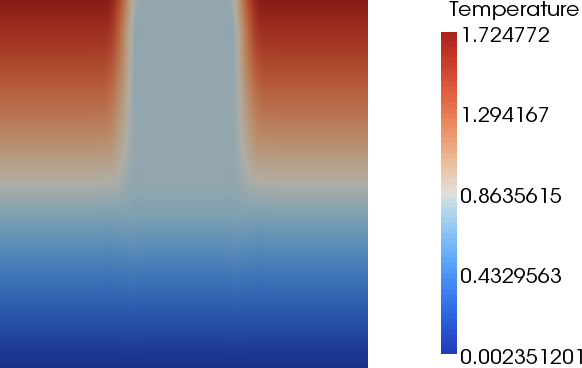
\includegraphics[width=10cm]{examples_images/restratification_after_oodc/rousset-init.png}
\caption{A vertical slice throught the domain showing the initial temperature stratification. The domain is a cylinder of radius 250 km and height 1 km. }
\label{fig:rousset-init}
\end{center}
\end{figure}


The mesh used is a layered mesh, which is created within fluidity from the two dimensional input mesh circle.*. The unstructured triangular mesh is extruded in the vertical, forming triangular prisms which are then divided into unstructured tetrahedra. The columnar arrangement of the nodes is important because the problem has a large aspect ratio, and the elements themselves are wider than they are tall. A fully unstructured mesh would create errors in the pressure, which then cause errors in the velocity. The layered mesh may be considered to be a special case of the two plus one mesh, in which the nodes are still vertically aligned, but there are different amounts of resolution in different areas of the domain. The resolution is 5 km in the horizontal and 83 m in the vertical. 


The velocity is solved for using a discontinuous galerkin discretisation to make the results more accurate. A continuous galerkin discretisation is used for both pressure and temperature, with a polynomial order of 2 for pressure and 1 for temperature.  This discretisation is sometimes referred to as p1dgp2. For this discretisation, the quadrature degree has to be set to 4.   To make it more stable, subcycling is switched on under velocity with a maximum courant number per subcycle of 0.1. There is a diagnostic free surface field which requires a free surface boundary condition under Velocity.

The timestep is 7200 s and there are two non-linear iterations.  The timestep is constrained by the courant condition, but is allowed to be bigger that would otherwise be expected because  an Absorption field is added under Velocity.  If this field was not added the time steps would be limited by the scale of the baroclinic waves.  This term has a vertical component equal to  ${\frac{1}{\rho_0}} {\theta} {\Delta} {t} {g} {\frac{\partial \rho}{\partial z}}$ and the other components are zero. $\rho_0$ is the reference density, $\theta$ is the value set under \\* \option{\ldots/Velocity/temporal\_discretisation/theta}, ${\Delta} {t} $ is the timestep, $g$ is the acceleration due to gravity and $\frac{\partial \rho}{\partial z}$ is the background density stratification.   In this case the absorption term is $0.025$ in the vertical and $0.0$ in the horizontal. The \\* \option{\ldots/Absorption/include\_pressure\_correction} option is turned on. 

\subsection{Results}

Figure \ref{fig:rousset-40m} shows the temperature field for a cross section at 40 m depth at 5 day intervals. As the column mixes with the surroundings, eddies are seen to form. If this is run with a different resolution a different number of eddies may form. If the resolution is too coarse then no eddies will form at all.

You might wish to try spinning up before you run this problem.  First run to a steady state with fixed temperature and then run the prognostic simulation from your checkpoints.

\begin{figure}[h!]
\begin{center}
\subfigure [0 days]{
\includegraphics[width=5cm]{examples_images/restratification_after_oodc/5000/rousset-res5000-depth-40m0001.png}}
\subfigure [5 days]{
\includegraphics[width=5cm]{examples_images/restratification_after_oodc/5000/rousset-res5000-depth-40m0002.png}}
\subfigure [10 days]{
\includegraphics[width=5cm]{examples_images/restratification_after_oodc/5000/rousset-res5000-depth-40m0003.png}}
\subfigure [15 days]{
\includegraphics[width=5cm]{examples_images/restratification_after_oodc/5000/rousset-res5000-depth-40m0004.png}}
\subfigure [20 days]{
\includegraphics[width=5cm]{examples_images/restratification_after_oodc/5000/rousset-res5000-depth-40m0005.png}}
\subfigure [25 days]{
\includegraphics[width=5cm]{examples_images/restratification_after_oodc/5000/rousset-res5000-depth-40m0006.png}}
\subfigure [30 days]{
\includegraphics[width=5cm]{examples_images/restratification_after_oodc/5000/rousset-res5000-depth-40m0007.png}}
\subfigure [35 days]{
\includegraphics[width=5cm]{examples_images/restratification_after_oodc/5000/rousset-res5000-depth-40m0008.png}}
\subfigure [40 days]{
\includegraphics[width=5cm]{examples_images/restratification_after_oodc/5000/rousset-res5000-depth-40m0009.png}}
\caption{The temperature cross-section at a depth of 40m.}
\label{fig:rousset-40m}
\end{center}
\end{figure}

%%%%%%%%%%%%%%%%%%%%%%%%%%%%%%%%%%%%%%%%%%%%%%%%%%%%%%%%%%%%%%%%%%%
%---Tides in the Mediterranean Sea--------------------%
%%%%%%%%%%%%%%%%%%%%%%%%%%%%%%%%%%%%%%%%%%%%%%%%%%%%%%%%%%%%%%%%%%%


\section{Tides in the Mediterranean Sea}
\label{sect:tides_in_the_med}

\subsection{Overview}

Tidal modelling is a widely used method for validating free surface implementations \citep{Shum1997}. The Mediterranean Sea
is a good example as it requires both astronomical and co-oscillating boundary tide forcing to obtain
an accurate solution \citep{Tsimplis1995, Wells2008}. An abundance of available tide gauge data recording the 
harmonic constants for both the amplitude and phase of a wide variety of different tidal constituets
facilitates comparisons between ICOM and real-world data. 
 

\subsection{Configuration}

The domain extends from 8$^\circ$W to 40$^\circ$E and from 28$^\circ$N to 48$^\circ$N with an open boundary adjacent to the Atlantic
Ocean in the west. The fixed mesh was generated using gmsh with shoreline data taken from the intermediate resolution $gshhs$
dataset (see \url{http://www.ngdc.noaa.gov/mgg/shorelines/gshhs.html}). The single-element deep tetrahedal elements were then
extruded in the vertical to fit a 3 arc-minute resolution bathymetric profile subsampled from the 1 arc-minute GEBCO dataset     
(see \url{http://www.gebco.net/}). A minimum depth of 3 m  is set to prevent wetting-and-drying related numerical instabilities.

The model is is driven by both astronomical and co-oscillating boundary tide forcing (see sections \ref{astronomical} and \ref{sec:boundary_tide})
for the four main tidal constituents; M$_{\text{2}}$, S$_{\text{2}}$, K$_{\text{1}}$ and O$_{\text{1}}$ (see \citealp{Schwiderski1980,Wells2008}).
Boundary tide data is sourced from the highly accurate FES2004 model \citep{Lyard2006} which is read in from a NetCDF file (see section\ref{Sect:BCs:specialised}). 
Frictional drag is applied as a surface-integral boundary condition to the bottom and sides and is based on a quadratic friction law 
of the form $-C_{D}|u|u$, where $C_{D}$ is the drag coefficient, $u$ is the velocity vector 
(ms$^{\text{-1}}$) and $|u|$ is the magnitude of the velocity vector ($|u|=\sqrt{u_{c}^{2}+v_{c}^{2}+w_{c}^{2}}$ where $u_{c}$ is the $x$ component of 
velocity (ms$^{\text{-1}}$), 
$v_{c}$ is the $y$ component of velocity (ms$^{\text{-1}}$) and $w_{c}$ is the 
$z$ component of velocity (ms$^{\text{-1}}$) respectively). 
The $C_{D}$ is set 0.0025, a value considered suitable for the majority of numerical ocean tidal models \citep{Wells2008}. 

The model outputs the harmonic constants for the amplitude and phase of each constituent as calculated from a time series using the least-squares
method. The timestep is 200 entries in length with data recorded every 5 timesteps after an initial spin up period of 20 hours (simulated time). 
The timestep itself is 5 minutes. The total runtime is 200 hours (simulated time).


\subsection{Results}

The harmonic amplitudes are presented as plotted scalar fields and compared with a high-resolution 2D model of \citet{Tsimplis1995} in
Figure \ref{amp}. The model results are similar to those of \citet{Tsimplis1995} and generally predict the correct patterns. 
The semidiurnal consitieunts give very similar results due to their similar frequencies (Figure \ref{amp}A - D). The amphidromic
systems are correctly located in the Sicilian Channel bewtween Sicily and Libya     
and in the northern Adriatic. The degenerate amphidromes are also accurately positioned near the Balearic Islands and in bewteen
Crete and Libya. The model also captures the amplification of the tidal amplitudes in both the Gulf of gables and the northern Adriatic, 
a phenomena primarilly due to resonance of the wave in these regions.

The amplitudes for the diurnal constituents show a similarly good match with the results of \citet{Tsimplis1995} (Figure \ref{amp}E - H).
The lowest amplitudes occur in the eastern part of the basin and there is pronounced amplification in the Adriatic Sea caused by this region
acting as a quarter-wave oscillator with the diurnal frequency \citep{Wells2008}. The degenerate amphidrome
along the Libyan coast (around the Gulf of Sirte) is correctly predicted.   

\begin{figure}[t!]
\centering
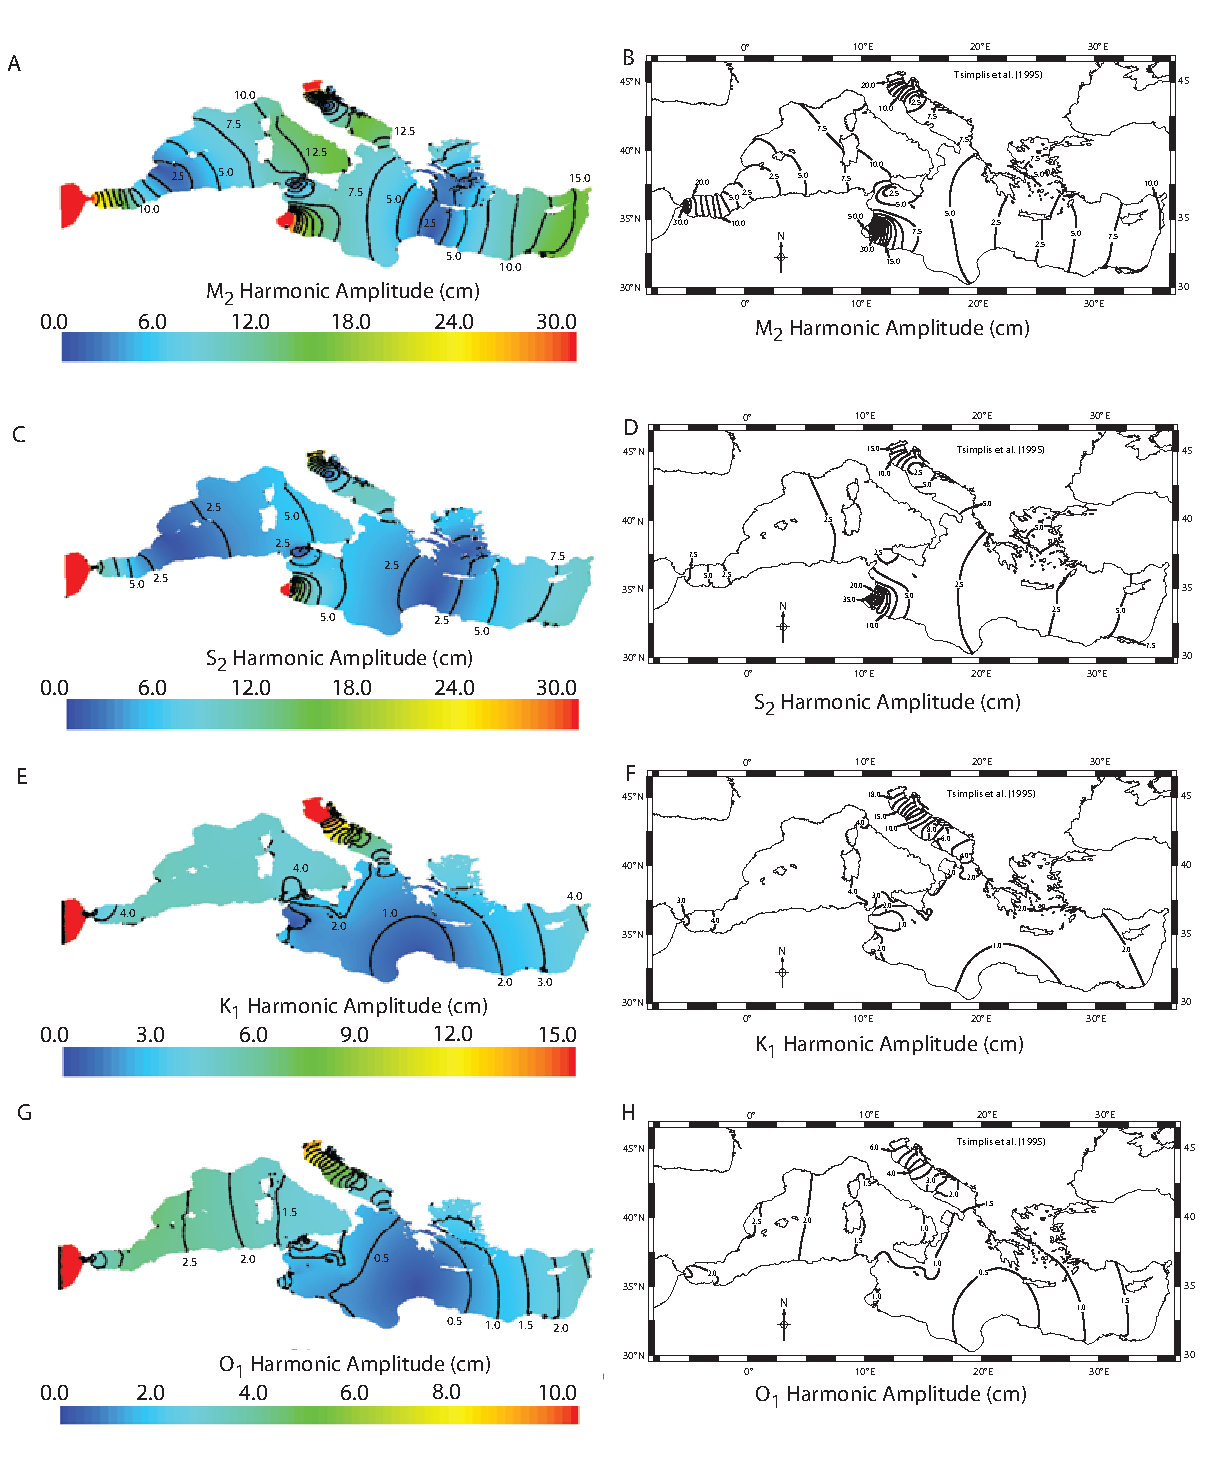
\includegraphics[width=\textwidth]{./examples_images/tides_in_the_Mediterranean_Sea/amp.pdf}
\caption{Plots of the tidal harmonic amplitudes in the Mediterranean Sea from ICOM and the high resolution
model of \citet{Tsimplis1995}.}
\label{amp}
\end{figure}

\begin{figure}[t!]
\centering
\includegraphics[width=\textwidth]{./examples_images/tides_in_the_Mediterranean_Sea/phase.pdf}
\caption{Plots of the tidal harmonic phases in the Mediterranean Sea from ICOM and the high resolution
model of \citet{Tsimplis1995}. } 
\label{phase}
\end{figure}

The phases as predicted by ICOM and by \citet{Tsimplis1995} are presented in Figure \ref{phase}. These show
a general agreement with the amphidromic systems shown to be rotating in an anti-clockwise direction; a feature
brought about by Coriolis force deflecting the tidal wave to the right in the Northern Hemisphere.
ICOM appears to slightly overpredict the wave speed in all cases; a result that could be attributed to any number of eatures including the
bathymetric/mesh reolution and/or an insufficntly low drag coefficient. Another possible source of error is that the
phase of the boundary tide and the natural mode of oscillation of the basin might not be synchronised; something that
\citet{Tsimplis1995} adjusted repeatedly until they achieved their best results.
 
The harmonic amplitudes are compared with data from 62 tide gauges (Figure \ref{gauge}; \citealp{Tsimplis1995,Wells2008}).
The RMS differences for ICOM are typically 2-3 times those of \citet{Tsimplis1995}    
with the largest errors being for the diurnal constituents (Table \ref{rms}). Despite these discrepencies, the
magnitudes of the RMS differences indicate a good match with the tide gauges, even in a strongly microtidal environment 
such as the Mediterranean Sea. 

\begin{figure}[htbp]
\centering
\includegraphics[width=\textwidth]{./examples_images/tides_in_the_Mediterranean_Sea/gauges.pdf}
\caption{Locations of 62 tide gauges in the Mediterranean Sea. Modified from \citet{Wells2008} with data originally taken from 
\citet{Tsimplis1995}. }
\label{gauge}
\end{figure}

\begin{table}[htbp]
\centering
\begin{tabular}{l c c}
\hline
\bf{Tidal Constituent} & \multicolumn{2}{c}{\bf{RMS Differences}} \\
\cline{2-3}
& \bf{\citet{Tsimplis1995}} & \bf{ICOM} \\
\hline
M$_{\text{2}}$ &1.37 & 3.8\\
S$_{\text{2}}$ &0.68 & 2.4\\
K$_{\text{1}}$ &0.82 & 1.5\\
O$_{\text{1}}$ &0.34 & 1.3\\
\hline
\end{tabular}
\caption{RMS differences between modelled harmonic amplitudes and real-world data from 62 tide gauges.
Data is presented from \citet{Tsimplis1995} and ICOM. }
\label{rms}
\end{table}

The quality of the match is further highlighted in scatter diagrams plotting 
the harmonic amplitudes from ICOM at each gauge location against the tide gauge data (Figure \ref{plots}).
These reveal how although ICOM tends to marginally overpredict the amplitude there is a strong
positive correlation closely delineating $y=x$. 

\begin{figure}[t]
\centering
\includegraphics[width=\textwidth]{./examples_images/tides_in_the_Mediterranean_Sea/plots}
\caption{Scatter diagrams plotting harmonic amplitudes from ICOM at each gauge location against tide gauge data.} 
\label{plots}
\end{figure}

%%%%%%%%%%%%%%%%%%%%%%%%%%%%%%%%%%%%%%%%%%%%%%%%%%%%%%%%%%%%%%%%%%%
%---------------------HOKKAIDO-NANSEI-OKI TSUNAMI-----------------%
%%%%%%%%%%%%%%%%%%%%%%%%%%%%%%%%%%%%%%%%%%%%%%%%%%%%%%%%%%%%%%%%%%%

\section{Hokkaido-Nansei-Oki tsunami}
\label{sect: hokkaido-nansei-oki_tsunami}

\subsection{Overview}
The Okushiri tsunami in 1993 is a tsunami event which produced run-up heights of up to $30$m in Okushiri island, Japan. 
The Research Institute for Electric Power Industry (CRIEPI) in Abiko, Japan constructed a $1/400$ laboratory model of the area around the island \cite{androsov2008tsunami}, which is used here as a benchmark problem. 

\subsection{Configuration}
The considered domain measures $5.448\mbox{m} \times 3.402\mbox{m}$  and the bathymetry and coastal topography of the experimental setup closely correspond to measurement data, see Figure \ref{pic:monai_inputwave} (a). 
On the left boundary, a prescribed surface elevation profile was enforced resembling a tsunami wave (Figure \ref{fig:monai_inputwave} (a)). 
The remaining boundaries were solid.
Three surface elevation gauge stations, marked as dots in Figure \ref{fic:monai_inputwave} (a), were deployed in the experiment.
\begin{figure}
\begin{center}
\includegraphics[width=0.7\textwidth]{./examples_images/hokkaido-nansei-oki_tsunami/MonaiValleyDomainWithInputWave2_png.pdf}
\end{center}
\caption{The bathymetry and the three gauge stations (a) and the horizontal mesh (b) used for the Okushiri tsunami test case.}\label{fig:monai_inputwave}
\end{figure}

The numerical simulation uses the same domain dimensions and bathymetry as the experiment. 
The vertically aligned, one element deep and horizontally unstructured mesh consists of $19,464$ tetrahedral elements with increased resolution near the inundation areas, see Figure \ref{pic:monai_inputwave} (b). 
The equations are solved with the $P_1-P_1$ finite element pair, a backward Euler time discretisation with a time-step of $0.1$s and $d_0=0.5$mm. 
The isotropic kinematic viscosity and gravity magnitude are set to $0.01\mbox{m}^{2}\mbox{s}^{-1}$ and $9.81\mbox{ms}^{-2}$, respectively.
On the left boundary the tsunami wave shown in \ref{pic:monai_results} (a) is prescribed and no-normal flow boundary conditions are applied at the other sides of the domain and the bottom to resemble the solid boundaries in the experiment.
In addition, a Manning-Strickler drag is used at the bottom with $n=0.002\mbox{sm}^{-\frac{1}{3}}$.
To prevent wave breaking in the simulation, this coefficient is increased to $0.2\mbox{sm}^{-\frac{1}{3}}$ in a rectangular area with a side length of $0.5$m centred at $3.4$m $\times 1.7$m (which is the centre of the island in the domain) and a fourth order stabilization is applied, see \cite{pain2001tetrahedral, piggott2008new}.

\subsection{Results}
The results at the gauge station plotted against the laboratory measurements are shown in Figure \ref{fic:monai_results} (b). 
\begin{figure}
\begin{center}
\includegraphics[width=\textwidth]{./examples_images/hokkaido-nansei-oki_tsunami/MonaiValley_C_p1p1_nu0_01_kmkstab_drag0_002_butcircularoundisland0_2-crop-crop_final2.pdf}
\caption{The input wave elevation of the Okushiri tsunami test case (a) and the numerical and experimental results at ``Gauge 1'' (top), ``Gauge 2'' (middle) and ``Gauge 3'' (bottom) (b).}\label{fig:monai_results}
\end{center}
\end{figure}

\subsection{Exercises}
\begin{enumerate}
\item Examine the way that the $u=1$ lid condition is applied in the flml file. Why has it not been set as simply a constant?
Try changing it to a constant and see what happens to the errors that you achieve. [Hint: some people consider the "regularised" 
lid-driven cavity problem. Try finding some papers that discuss this, and update the boundary condition so it matches the 
regularised problem. Compare to benchmark data if you can find it].
\item The references given above include data from other Reynolds numbers. Try updating the problem set-up and the post-processing script which computes
the errors for a higher Reynolds number.
\item Try switching on mesh adaptivity (you will need to ensure that you have configured your \fluidity\ executable with \texttt{--enable-2d-adaptivity}). 
Test adapting based on different metrics, e.g. try weighting $u$, $v$ and $p$
differently and see what meshes you get. Try varying these weights as well as the maximum and minimum allowed element
sizes to see how they affect each other and the mesh that results. Can you get a metric that results in a lower
error for the same number of nodes compared to the fixed mesh (hint: it may be easier to achieve this at higher Reynolds numbers)?.
\end{enumerate}



% Whole bunch of format hacking because Bibliography isn't a real chapter.
\cleardoublepage
\phantomsection
\renewcommand\leftmark{}
\renewcommand\rightmark{Bibliography}
\addcontentsline{toc}{chapter}{Bibliography}
\bibliography{bibliography}

\appendix

\chapter{About this manual}\label{App:about}

\section{Introduction}

This document attempts to give an introduction to the use of the
\fluidity/ICOM code for CFD and ocean modelling applications.  The layout of this manual
is briefly covered in the overview at the beginning of this document.

Although this document may of course be printed, viewing it on screen may be
wise as it allows colour images to be viewed, and links between sections and
parameters should work. Also, where possible figures are `vectorised' so
that if viewed electronically it is possible to zoom right in to see the
structure of meshes for example.

This manual is very much a work in progress. Therefore spelling, grammar,
and accuracy can not be guaranteed. Users with commit access to the \fluidity\
source tree are encouraged to make contributions directly. Other users are
invited to email comments, corrections and contributions to
\verb|m.d.piggott@imperial.ac.uk|

A further source of material may be found at \url{http://amcg.ese.ic.ac.uk/}
This points to a collection of wiki web pages that all users are able to
update and add to. 

\section{Audience and Scope}

The manual is primarily designed to enable \fluidity\ users to run \fluidity\
effectively. As such, this is the appropriate place for documentation
concerning the available configuration options of the model and the correct
method of employing them. It is also the correct place to document the
mathematical formulation of the model and the equations which it
solves. Other matters which should be covered include input and output
formats, checkpointing and visualisation.

This is not generally the appropriate forum for low-level documentation
directed at model developers. Information concerning the finite element
method and its implementation in \fluidity\ should be placed in the Femtools
manual while other implementation details could be placed on the AMCG wiki.

\section{Style guide}

\subsection{Headings}

Headings should be typeset with sentence capitalisation. That is to say,
only those words which would be capitalised if the heading were an ordinary
sentence are capitalised.

\subsection{Language}

The manual is written in British English. This, among many distinctions from
our cousins across the Pond means:

\begin{itemize}
\item centre not center.
\item visualise not visualize.
\item licence for the noun, license for the verb.
\end{itemize}

\subsection{Labelling}

Sections, tables, figures and equations should be labelled consistenly.

Sections should be labelled as \verb+\label{sec:unique_section_name}+, 
tables should labelled as \verb+\label{tab:unique_table_name}+, figures as
\verb+\label{fig:unique_figure_name}+, and equations as 
\verb+\label{eq:unique_equation_name}+.

Note that all label names should be unique across the manual.

\subsection{Images}

The manual is designed to be compilable to both PDF and html. This creates
particular challenges when incorporating images. One approach which is
particularly appropriate for diagrams and other images annotated with text
or equations is to generate or annotate the figures using xfig. Xfig files
may be automatically converted to Postscript for the PDF document and png
for the html version. If the ``special'' attribute is set on text in the
xfig document, then that text will be rendered in \LaTeX. This in particular
enables equations to be included in figures in a manner consistent with the
equations in the text.

\subsubsection{Including xfig images}

This manual defines the command \lstinline[language=TeX]+\xfig{basename}+
which will import \verb+basename.pdftex_t+ for pdf output and
\verb+basename.png+ for web output. Authors should ensure that their xfig
file has the name \verb+basename.fig+ and that \verb+basename+ is added to
the \verb+XFIG_IMAGES+ variable in the \verb+Makefile+. This will cause the
commands \verb+make fluidity_manual.pdf+ and
\verb+make fluidity_manual.html+ to also generate the pdf and png versions
of the figure respectively.

It will be observed that the \verb+\xfig+ command does not take any arguments
for figure size. This is a deliberate decision designed to ensure that the
font size matches between the figure and the text. Figures should instead be
appropriately sized in xfig.

\subsubsection{Including other figures}

For other figures, the command
\lstinline[language=TeX]+\fig[options]{basename}+ is provided. In this case,
it is the author's responsibility to provide both \verb+basename.pdf+ and
\verb+basename.png+ files. Please add \verb+basename+ to the \verb+IMAGES+
variable in the \verb+Makefile+. This will cause the image files to become
dependencies of the compiled manual.

If no \verb+basename.png+ is available, then the
\lstinline[language=TeX]+\pdffig[options]{basename}+ should be used instead.

The \lstinline[language=TeX]+options+ provided to
\lstinline[language=TeX]+\fig+ are passed straight to
\lstinline[language=TeX]+\includegraphics+ and may therefore include any
options which are legal in that context including resizing options.

\subsection{flml options}

The \verb+\option+ command is provided to format \fluidity\ option
paths. Options should be formatted according to normal Spud conventions
however it will frequently be desirable to show partial option paths not
starting from the root. In this circumstance, an ellipsis should be used to
show an unknown path component. For example, the mesh element of some
prescribed field would be \option{\ldots/prescribed/mesh} which can be input
in \LaTeX\ as \lstinline[language=TeX]+\option{\ldots/prescribed/mesh}+

\subsection{Generating pdf and html output}

The manual may be compiled to both pdf and html. For the former, type:
\begin{lstlisting}[language=bash]
  make fluidity_manual.pdf
\end{lstlisting}
and for the latter type:
\begin{lstlisting}[language=bash]
  make fluidity_manual.html
\end{lstlisting}
It may sometimes be necessary to introduce content which should only be
rendered in one or other output format. For example, long option paths
frequently defeat \LaTeX's line breaking algorithm so it may be necessary to
force line breaks in the pdf document. Since the browser is responsible for
line breaks in html, it would be inappropriate to force a linebreak in the
html output. For this purpose, the manual provides the commands
\lstinline[language=TeX]+\ifhtml{content for html}{content for pdf}+ as well
as the commands \lstinline[language=TeX]+\onlyhtml+ and
\lstinline[language=TeX]+\onlypdf+. The latter two commands take a single
argument which is only rendered for the applicable output.

\subsection{Representing source code}

Source code and commands entered in the shell can be typeset using the
\lstinline[language=TeX]+lstlisting+ environment. The environment typesets
its argument literally so unlike normal \LaTeX, spaces and carriage returns
are replicated in the output. The environment takes optional configuration
parameters of which the most important is 
\lstinline[language=TeX]+language+ which is used to select the programming
language. \LaTeX will highlight the syntax of the chosen language. Inline
commands can be typeset using\linebreak
\lstinline[language=TeX]*\lstinline[language=TeX]+command+* substituting any
applicable language. 

\subsubsection{Shell commands}

For shell commands, \lstinline[language=TeX]+language+ should be set to
\lstinline[language=TeX]+bash+. For example:
\begin{verbatim}
\begin{lstlisting}[language=bash]
dham@popper traffic > ls
box.ele   fluidity.err-0  Makefile       traffic_1.vtu  traffic.xml
box.face  fluidity.log-0  src            traffic.flml   vaf.bin
box.node  gmon.out        traffic_0.vtu  traffic.stat   vaf.dat
\end{lstlisting}
\end{verbatim}
will be rendered:
\begin{lstlisting}[language=bash]
dham@popper traffic > ls 
box.ele   fluidity.err-0  Makefile       traffic_1.vtu  traffic.xml
box.face  fluidity.log-0  src            traffic.flml   vaf.bin
box.node  gmon.out        traffic_0.vtu  traffic.stat   vaf.dat
\end{lstlisting}

\subsubsection{Other languages}

The other languages which are currently enabled are
\lstinline[language=TeX]+TeX+, for \LaTeX, \lstinline[language=TeX]+Python+,
\lstinline[language=TeX]+Make+ and \lstinline[language=TeX]+XML+. Many other
languages are supported by the \lstinline[language=TeX]+listings+ package.

\subsection{Bibliography}

Citations from the literature should be included whenever relevant. When
formatting entries in the bibliography database,
\lstinline[language=Bash]+bibliography.bib+, the preferred key is the first
author's surname in lower case followed by the full year of publication. For
example \lstinline[language=TeX]+ham2009+. The bibliography database should
be sorted alphabetically by key.

The manual uses an author-date citation style which means that it is
important to use the correct combination of
\lstinline[language=TeX]+\cite+,  \lstinline[language=TeX]+\citep+ and
\lstinline[language=TeX]+\citet+. See the \LaTeX\ \lstinline[language=TeX]+natbib+
 package documentation for more details.

\subsection{Mathematical notation conventions}

\subsubsection{Continuous Vectors and tensors}

There are two conceptually different forms of vector and tensor which occur
in the finite element method. The first is for quantities, such as velocity,
which are vector-valued in the continuum. These should be typeset in italic
bold: $\bmu$. The \lstinline[language=TeX]+\vec+ command has been redefined
for this purpose so a vector quantity named $\vec{b}$ would be typed
\lstinline[language=TeX]+\vec{b}+. However, a large number of
frequently-used vector quantities have convenience functions pre-defined in
\lstinline[language=bash]+notation.tex+. These have the name
\lstinline[language=TeX]+\bm+\textit{n}\ where \textit{n}\ is the symbol to
be typeset. Examples include \lstinline[language=TeX]+\bmu+ ($\bmu$) and
\lstinline[language=TeX]+\bmphi+ ($\bmphi$).

Continuous tensors are represented using a double overbar:
$\tensor{\tau}$. The \lstinline[language=TeX]+\tensor+ command is provided
for this purpose. Once again, convenience functions are provided for common
tensors, this time with the form
\lstinline[language=TeX]+\+\textit{n}\lstinline[language=TeX]+tens+ for
example \lstinline[language=TeX]+\tautens+ ($\tautens$) and
\lstinline[language=TeX]+\ktens+ ($\ktens$).

\subsubsection{Discrete vectors and matrices}

Vectors composed of the value of a field at each node and matrices mapping
between discrete spaces should be typeset differently from continuous
vectors and tensors. Discrete vectors should be typeset with an underline
using the \lstinline[language=TeX]+\dvec+ command. Note that the convention
in Fluidity is that vector fields are represented as scalar sums over vector
valued basis functions so the correct representation of the discrete
velocity vector is \lstinline[language=TeX]+\dvec{\bmu}+ ($\dvec{u}$).

Matrices should be typeset as upright upper case letters. The
\lstinline[language=TeX]+\mat+ command is available for this purpose. For
example \lstinline[language=TeX]+\mat{M}+ produces $\mat{M}$.

\subsubsection{Derivatives}

The full derivative and the material derivative should be typeset using an
upright $\d$ and $\D$ respectively. The \lstinline[language=TeX]+\d+ and
\lstinline[language=TeX]+\D+ commands are provided for this purpose. There
are also a number of functions provided for typesetting derivatives. Each of
these functions has one compulsory and one optional argument. The
compulsory argument is the function of which the derivative is being taken,
the optional argument is the variable with respect to which the derivative
is being taken. So, for example \lstinline[language=TeX]+\ppt[q]{y}+ gives:
\begin{equation*}
  \ppt[q]{y}.
\end{equation*}
While simple \lstinline[language=TeX]+\ppt{}+ gives:
\begin{equation*}
  \ppt{}.
\end{equation*}
Table \ref{tab:derivatives}\ shows the derivative functions available.
\begin{table}[ht]
  \centering
  \begin{tabular}{lc}
    \textbf{command} & \textbf{example}\\\hline
    \lstinline[language=TeX]+\ddx[]{}+ & \rule{0pt}{4ex}$\displaystyle\ddx{}$\\
    \lstinline[language=TeX]+\ddxx[]{}+ & \rule{0pt}{4ex}$\displaystyle\ddxx{}$\\
    \lstinline[language=TeX]+\ddt[]{}+ & \rule{0pt}{4ex}$\displaystyle\ddt{}$\\
    \lstinline[language=TeX]+\ddtt[]{}+ & \rule{0pt}{4ex}$\displaystyle\ddtt{}$\\
    \lstinline[language=TeX]+\ppx[]{}+ & \rule{0pt}{4ex}$\displaystyle\ppx{}$\\
    \lstinline[language=TeX]+\ppxx[]{}+ & \rule{0pt}{4ex}$\displaystyle\ppxx{}$\\
    \lstinline[language=TeX]+\ppt[]{}+ & \rule{0pt}{4ex}$\displaystyle\ppt{}$\\
    \lstinline[language=TeX]+\pptt[]{}+ & \rule{0pt}{4ex}$\displaystyle\pptt{}$\\
    \lstinline[language=TeX]+\DDx[]{}+ & \rule{0pt}{4ex}$\displaystyle\DDx{}$\\
    \lstinline[language=TeX]+\DDxx[]{}+ & \rule{0pt}{4ex}$\displaystyle\DDxx{}$\\
    \lstinline[language=TeX]+\DDt[]{}+ & \rule{0pt}{4ex}$\displaystyle\DDt{}$\\
    \lstinline[language=TeX]+\DDtt[]{}+ & \rule{0pt}{4ex}$\displaystyle\DDtt{}$\\ 
  \end{tabular}
  \caption{Functions for correctly typesetting derivatives.}
  \label{tab:derivatives}
\end{table}

\subsubsection{Integrals}

Integrals in any number of dimensions should be typeset with an integral
sign and no measure (\ie no $\d x$ or $\d V$). The domain over which the
integral is taken should be expressed as a subscript to the integral sign
itself. The integral of $\psi$ over the whole domain will therefore be
written as:
\begin{equation*}
  \int_\Omega \psi.
\end{equation*}

\subsubsection{Units}

Units should be typeset in upright font. The \LaTeX\ package
\lstinline+units+ does this for you automagically. The correct syntax is
\lstinline[language=TeX]+\unit[value]{unit}+. For example
\lstinline[language=TeX]+\unit[5]{m}+ produces \unit[5]{m}. There are a
number of convenience functions defined for the manual to make this job
easier. These are shown in table \ref{tab:units}. Providing the value as an
argument to the unit ensures that the spacing between the value and the unit
is correct and will not break over lines. The value is an optional argument
so if there is no value, just leave it out. \lstinline+units+ does the right
thing in both text and math modes. Other convenience functions can easily be
added to \lstinline[language=bash]+notation.tex+.
\begin{table}[ht]
  \centering
  \begin{tabular}{lcc}
    \textbf{command} & \textbf{example}\\\hline
    \lstinline[language=TeX]+\m[length]+ & \m[1] \\
    \lstinline[language=TeX]+\km[length]+ & \km[1] \\
    \lstinline[language=TeX]+\s[time]+ & \s[1] \\
    \lstinline[language=TeX]+\ms[speed]+ & \ms[1] \\
    \lstinline[language=TeX]+\mss[accel]+ & \mss[1] \\
    \lstinline[language=TeX]+\K[temp]+ & \K[1] \\
    \lstinline[language=TeX]+\PSU[salin]+ & \PSU[1] \\
    \lstinline[language=TeX]+\Pa[press]+ & \Pa[1] \\
    \lstinline[language=TeX]+\kg[mass]+ & \kg[1] \\
    \lstinline[language=TeX]+\rads[ang_vel]+ & \rads[1] \\
    \lstinline[language=TeX]+\kgmm[density]+ & \kgmm[1] \\
  \end{tabular}
  \caption{Convenience functions for physical units}
  \label{tab:units}
\end{table}


\subsubsection{Abbreviations in formulae}

Abbreviations in formulae should be typeset in upright maths mode using
\lstinline[language=TeX]+\mathrm+. For example
\lstinline[language=TeX]+F_{\mathrm{wall}}+ ($F_{\mathrm{wall}}$).  

\chapter{Mathematical notation}

The table below gives a description of some of the commonly used symbols in this manual.
Note that some symbols are used to denote multiple concepts, and therefore there are some repeated
entries.

\begin{center}
\begin{longtable}{cl}
\hline\hline
Symbol & Definition\\
\hline\hline
\endfirsthead
%
\multicolumn{2}{c}{{\tablename} -- Continued} \\[0.5ex]
\hline\hline
Symbol & Definition\\
\hline\hline
\endhead
%This is the footer for all pages except the last page of the table...
  \\[0.5ex]
  \multicolumn{2}{l}{{Continued on Next Page\ldots}} \\
\endfoot
%This is the footer for the last page of the table...
  \hline
\endlastfoot
%
%
\multicolumn{2}{l}{{\bf Mathematical symbols}} \\ \hline
%
$\nabla$     & gradient operator \\
$\partial$   & domain boundary \\
\hline
%
\multicolumn{2}{l}{{\bf Greek}} \\ \hline
%
$\alpha$     & thermal expansion coefficient\\
$\beta$      & saline contraction coefficient\\
$\gamma$     & isothermal compressibility coefficient\\
$\eta$       & free surface height\\
$\eta_{\textrm{eq}}$ & equilibrium tide\\
$\kaptens$   & diffusivity tensor\\
$\lambda$    & longitude\\
$\mu$        & dynamic or molecular viscosity\\
$\nu$        & kinematic viscosity\\
$\phi$       & latitude\\
$\phi$       & test function\\
$\psi$       & trial function\\
$\rho$       & density\\
$\rho_0$     & constant background density\\
$\rho'$      & perturbation density\\
$\sigtens$   & stress tensor\\
$\bmtau$     & unit tangent vector\\
$\bmOmega$   & rotation vector\\
\hline
%
\multicolumn{2}{l}{{\bf Latin}} \\ \hline
%
$\vec{b}$      & buoyancy vector\\
$c_p$       & specific heat constant\\
$e$         & specific internal energy\\
$E$         & total specific energy\\
$f$         & Coriolis parameter\\
$\bmg$      & gravity vector\\
$\ktens$    & thermal conductivity tensor\\
$\mat{M}$   & mass matrix\\
$\metric$   & metric tensor\\
$\bmn$      & unit normal vector\\
$p$         & pressure\\
$p_a$       & air pressure\\
$p_h$       & hydrostatic pressure\\
$p'$        & perturbation pressure\\
$\bmq$      & thermal conduction\\
$R_E$       & radius of the Earth\\
$s$         & entropy\\
$S$         & salinity\\
$T$         & temperature\\
$\bmu$      & velocity vector\\
$w$         & enthalpy\\


\end{longtable}
\end{center}

\chapter{Useful numbers}

The table below gives some useful physical values for parameters often used in modelling.

\begin{center}
\begin{longtable}{lll}
\hline
Definition & Symbol & Value\\
\hline
\endfirsthead
%
\multicolumn{2}{c}{{\tablename} -- Continued} \\[0.5ex]
\hline
Definition & Symbol & Value and units\\
\hline
\endhead
%This is the footer for all pages except the last page of the table...
  \\[0.5ex]
  \multicolumn{2}{l}{{Continued on Next Page\ldots}} \\
\endfoot
%This is the footer for the last page of the table...
  \hline
\endlastfoot
%
Radius of Earth (at equator)                    &  $R_E^{eq}$   &  $\m[6.3781\times 10^6]$\\
Radius of Earth (at pole)                       &  $R_E^{p}$    &  $\m[6.3568\times 10^6]$\\
Radius of Earth (average value)                 &  $R_E^{av}$   &  $\m[6.371\times 10^6]$\\
Mass of Earth                                   &  $M_E$        &  $\kg[5.9742\times 10^{24}]$\\
Mass of Moon                                    &  $M_M$        &  $\kg[7.36\times 10^{22}]$\\
Mass of Sun                                     &  $M_S$        &  $\kg[1.98892\times 10^{30}]$\\
Earth's rotation rate (based on sidereal day)   &  $\Omega$     &  $\rads[7.2921\times 10^{-5}]$\\
\end{longtable}
\end{center}

\chapter{Dimensional analysis}

\section{Non-dimensionalisation}
Consider system (\ref{boussinesq}) and rescale spatial lengths with the transformation
\begin{equation}
\tilde{x}=\frac{x}{L},\quad \tilde{y}=\frac{y}{L},\quad \tilde{z}=\frac{z}{H},
\end{equation}
where $\tilde{x},\tilde{y},\tilde{z}$ are nondimensional numbers and $L$ and $H$
are scaling values in the horizontal and vertical respectively. These generally take
typical values for length scales so that $\tilde{x},\tilde{y},\tilde{z}$ are ${\cal O}(1)$.

The momentum equations in (\ref{boussinesq}) then become (for simplicity dropping $\bmF$, $\hat{\bmu}$
and assuming that $2 \bmOmega \times \bmu=f\bmk\times\bmu$ and $\nabla\cdot \tautens = \nu\nabla^2\bmu$),
\begin{subeqnarray*}
\frac{\pp u}{\pp t}
+ L^{-1}u\frac{\pp u}{\pp\tilde{x}} + L^{-1}v\frac{\pp u}{\pp\tilde{y}} + H^{-1}w\frac{\pp u}{\pp\tilde{z}}
-fv
&=& -L^{-1}\frac{\pp p}{\pp\tilde{x}} - L^{-1}g\frac{\pp \eta}{\pp\tilde{x}}\\&&\quad
+L^{-2}\nu\frac{\pp^2 u}{\pp\tilde{x}^2}+L^{-2}\nu\frac{\pp^2 u}{\pp\tilde{y}^2}+H^{-2}\nu\frac{\pp^2 u}{\pp\tilde{z}^2},\\
\frac{\pp v}{\pp t}
+ L^{-1}u\frac{\pp v}{\pp\tilde{x}} + L^{-1}v\frac{\pp v}{\pp\tilde{y}} + H^{-1}w\frac{\pp v}{\pp\tilde{z}}
+fu
&=& -L^{-1}\frac{\pp p}{\pp\tilde{y}} - L^{-1}g\frac{\pp \eta}{\pp\tilde{y}}\\&&\quad
+L^{-2}\nu\frac{\pp^2 v}{\pp\tilde{x}^2}+L^{-2}\nu\frac{\pp^2 v}{\pp\tilde{y}^2}+H^{-2}\nu\frac{\pp^2 v}{\pp\tilde{z}^2},\\
\frac{\pp w}{\pp t}
+ L^{-1}u\frac{\pp w}{\pp\tilde{x}} + L^{-1}v\frac{\pp w}{\pp\tilde{y}} + H^{-1}w\frac{\pp w}{\pp\tilde{z}}
&=& -H^{-1}\frac{\pp p}{\pp\tilde{z}} - \rho g\\&&\quad
+L^{-2}\nu\frac{\pp^2 w}{\pp\tilde{x}^2}+L^{-2}\nu\frac{\pp^2 w}{\pp\tilde{y}^2}+H^{-2}\nu\frac{\pp^2 w}{\pp\tilde{z}^2}.
\end{subeqnarray*}

Now suppose that we also have representative velocity scales in the horizontal and vertical ($U,W$) and
define
\begin{equation}
\tilde{u}=\frac{u}{U},\quad \tilde{v}=\frac{v}{U},\quad \tilde{w}=\frac{w}{W},
\end{equation}
then substituting we have
\begin{subeqnarray*}
U\frac{\pp \tilde{u}}{\pp t}
+ U^2L^{-1}\left(\tilde{u}\frac{\pp \tilde{u}}{\pp\tilde{x}} + \tilde{v}\frac{\pp \tilde{u}}{\pp\tilde{y}}\right) + UWH^{-1}\tilde{w}\frac{\pp \tilde{u}}{\pp\tilde{z}}
-Uf\tilde{v}
&=& -L^{-1}\frac{\pp p}{\pp\tilde{x}} - L^{-1}g\frac{\pp \eta}{\pp\tilde{x}}\\&&\quad
+UL^{-2}\nu\left(\frac{\pp^2 \tilde{u}}{\pp\tilde{x}^2}+\frac{\pp^2 \tilde{u}}{\pp\tilde{y}^2}\right)+H^{-2}U\nu \frac{\pp^2 \tilde{u}}{\pp\tilde{z}^2},\\
U\frac{\pp \tilde{v}}{\pp t}
+ U^2L^{-1}\left(\tilde{u}\frac{\pp \tilde{v}}{\pp\tilde{x}} + \tilde{v}\frac{\pp \tilde{v}}{\pp\tilde{y}}\right) + UWH^{-1}\tilde{w}\frac{\pp \tilde{v}}{\pp\tilde{z}}
+Uf\tilde{u}
&=& -L^{-1}\frac{\pp p}{\pp\tilde{y}} - L^{-1}g\frac{\pp \eta}{\pp\tilde{y}}\\&&\quad
+UL^{-2}\nu\left(\frac{\pp^2 \tilde{v}}{\pp\tilde{x}^2}+\frac{\pp^2 \tilde{v}}{\pp\tilde{y}^2}\right)+H^{-2}U\nu\frac{\pp^2 \tilde{v}}{\pp\tilde{z}^2},\\
W\frac{\pp \tilde{w}}{\pp t}
+ UWL^{-1}\left(\tilde{u}\frac{\pp \tilde{w}}{\pp\tilde{x}} + \tilde{v}\frac{\pp \tilde{w}}{\pp\tilde{y}}\right) + W^2H^{-1}\tilde{w}\frac{\pp \tilde{w}}{\pp\tilde{z}}
&=& -L^{-1}\frac{\pp p}{\pp\tilde{z}} -  \rho g\\&&\quad
+WL^{-2}\nu\left(\frac{\pp^2 \tilde{w}}{\pp\tilde{x}^2}+\frac{\pp^2 \tilde{w}}{\pp\tilde{y}^2}\right)+H^{-2}W\nu\frac{\pp^2 \tilde{w}}{\pp\tilde{z}^2}.
\end{subeqnarray*}

Once representative length and velocity scales have been defined this automatically sets a temporal scale
\begin{equation*}
\tilde{t}=\frac{t}{T},\quad T=\frac{L}{U},
\end{equation*}
and the divergence-free continuity equation $\nabla\cdot\vec{u}=0$
suggests the scaling constraint
\begin{equation}
\frac{W}{H}=\frac{U}{L}.
\label{aspect99}
\end{equation}

Again, substituting and dividing through by $UT^{-1}$ in the horizontal and $WT^{-1}$
in the vertical, and making use of (\ref{aspect99}) yields
\begin{subeqnarray*}
\frac{\pp \tilde{u}}{\pp \tilde{t}}
+ \tilde{u}\frac{\pp \tilde{u}}{\pp\tilde{x}} + \tilde{v}\frac{\pp \tilde{u}}{\pp\tilde{y}} + \tilde{w}\frac{\pp \tilde{u}}{\pp\tilde{z}}
-\frac{Lf}{U}\tilde{v}
&=& -U^{-2}\frac{\pp p}{\pp\tilde{x}} - U^{-2}g\frac{\pp \eta}{\pp\tilde{x}}\\&&\quad
+U^{-1}L^{-1}\nu\left(\frac{\pp^2 \tilde{u}}{\pp\tilde{x}^2}+\frac{\pp^2 \tilde{u}}{\pp\tilde{y}^2}\right)+H^{-2}LU^{-1}\nu \frac{\pp^2 \tilde{u}}{\pp\tilde{z}^2},\\
\frac{\pp \tilde{v}}{\pp \tilde{t}}
+ \tilde{u}\frac{\pp \tilde{v}}{\pp\tilde{x}} + \tilde{v}\frac{\pp \tilde{v}}{\pp\tilde{y}} + \tilde{w}\frac{\pp \tilde{v}}{\pp\tilde{z}}
+\frac{Lf}{U}\tilde{u}
&=& -U^{-2}\frac{\pp p}{\pp\tilde{y}} - U^{-2}g\frac{\pp \eta}{\pp\tilde{y}}\\&&\quad
+U^{-1}L^{-1}\nu\left(\frac{\pp^2 \tilde{v}}{\pp\tilde{x}^2}+\frac{\pp^2 \tilde{v}}{\pp\tilde{y}^2}\right)+H^{-2}LU^{-1}\nu \frac{\pp^2 \tilde{v}}{\pp\tilde{z}^2},\\
\frac{\pp \tilde{w}}{\pp \tilde{t}}
+ \tilde{u}\frac{\pp \tilde{w}}{\pp\tilde{x}} + \tilde{v}\frac{\pp \tilde{w}}{\pp\tilde{y}} + \tilde{w}\frac{\pp \tilde{w}}{\pp\tilde{z}}
&=& -LH^{-1}U^{-1}W^{-1}\frac{\pp p}{\pp\tilde{z}} - LU^{-1}W^{-1}\rho g\\&&\quad
+U^{-1}L^{-1}\nu\left(\frac{\pp^2 \tilde{v}}{\pp\tilde{x}^2}+\frac{\pp^2 \tilde{v}}{\pp\tilde{y}^2}\right)+H^{-2}LU^{-1}\nu \frac{\pp^2 \tilde{v}}{\pp\tilde{z}^2}.
\end{subeqnarray*}

The Coriolis term takes the form
\begin{equation*}
\frac{Lf}{U}\bmk\times\tilde{\bmu}=\Ro^{-1}\bmk\times\tilde{\bmu}.
\end{equation*}
The buoyancy term takes the form
\begin{equation*}
\frac{L}{UW}\rho g = \frac{L}{H}\frac{U}{W}\Fr^{-1}\rho = \frac{L^2}{H^2}\Fr^{-1}\rho = \Delta^2\Fr^{-1}\rho.
\end{equation*}
The viscous term takes the form
\begin{equation*}
U^{-1}L^{-1}\nu\left(\frac{\pp^2 \tilde{u}}{\pp\tilde{x}^2}+\frac{\pp^2 \tilde{u}}{\pp\tilde{y}^2}\right)+H^{-2}LU^{-1}\nu \frac{\pp^2 \tilde{u}}{\pp\tilde{z}^2}
=\Re_H^{-1}\left(\frac{\pp^2 \tilde{u}}{\pp\tilde{x}^2}+\frac{\pp^2 \tilde{u}}{\pp\tilde{y}^2}\right) + \Re_V^{-1}\frac{\pp^2 \tilde{u}}{\pp\tilde{z}^2},
\end{equation*}
where $\Re_H=UL/\nu$ and $\Re_V=WH/\nu$. 
%Note that is would have been
%trivial in the above to use a tensor of viscosity values rather than a
%constant.  -- COLIN: not sure what this means
Rescaling the free surface height in terms of the vertical
coordinate ($\tilde{\eta}=\eta/H$) yields a free surface term
\begin{equation*}
\frac{Hg}{U^2}\nabla_{\tilde{x}}\tilde{\eta}=\Fr^{-1}\nabla_{\tilde{x}}\tilde{\eta}.
\end{equation*}

Dropping tildes and using $p=U^{-2}p$ we have finally that
\begin{subeqnarray*}
\frac{\pp {u}}{\pp {t}}
+ \bmu\cdot\nabla u
-\Ro^{-1}{v}
&=& \frac{\pp p}{\pp {x}} - \Fr^{-1}\frac{\pp \eta}{\pp {x}}
+\Re_H^{-1}\left(\frac{\pp^2 {u}}{\pp {x}^2}+\frac{\pp^2 {u}}{\pp {y}^2}\right)+ \Re_V^{-1}\frac{\pp^2 {u}}{\pp {z}^2},\\
\frac{\pp {v}}{\pp {t}}
+ \bmu\cdot\nabla v
+\Ro^{-1}{u}
&=& \frac{\pp p}{\pp {y}} - \Fr^{-1}\frac{\pp \eta}{\pp {y}}
+\Re_H^{-1}\left(\frac{\pp^2 {v}}{\pp {x}^2}+\frac{\pp^2 {v}}{\pp {y}^2}\right)+ \Re_V^{-1}\frac{\pp^2 {v}}{\pp {z}^2},\\
\frac{\pp {w}}{\pp \tilde{t}}
+ \bmu\cdot\nabla w
&=& -\Delta^2 \frac{\pp p}{\pp {z}} - \Delta^2 \Fr^{-1}g
+\Re_H^{-1}\left(\frac{\pp^2 {v}}{\pp {x}^2}+\frac{\pp^2  {v}}{\pp {y}^2}\right)+ \Re_V^{-1}\frac{\pp^2 {v}}{\pp {z}^2}.
\end{subeqnarray*}

%\begin{thm}[Buckingham-Pi Theorem]
%Why nondimensionalising can help reduce parameter phase space ... Barenblatt ...
%\end{thm}


\section{Dimensionless parameters}
Table \ref{table:dimensionless} gives some common non-dimensional numbers.
The following expressions are also useful
\begin{equation*}
N^2=-\frac{g}{\rho_0}\ddt[z]{\rho} \approx \frac{g}{\rho_0}\frac{\Delta\rho}{H}=\frac{g'}{H}
\end{equation*}
\begin{equation*}
g' =\frac{\Delta\rho}{\rho_0}g
\end{equation*}


\begin{table}[t]
\begin{center}
\begin{tabular}{lll} \hline
Name        &   Description         &   Form        \\  \hline
            &                           &               \\
Aspect ratio   &   Ratio of length scales   &   $\Delta=L/H$  \\
Reynolds    &   inertial/viscous        &   $\Re=UL/\nu$    \\
Rossby      &   inertial/Coriolis\footnotemark[6]            &   $\Ro=U/fL$      \\
Froude      &   inertial/gravitational\footnotemark[7] &   $\Fr=U^2/gH$    \\
Froude (internal)   &   inertial/buoyancy   &   $\Fr_{\mathrm{internal}}=U^2/g'H=U/NH$   \\
Burger      &  $\Bu=\Ro/\Fr$    &   $\Bu = NH/fL$  \\
Richardson  &   buoyancy/inertial\footnotemark[8]       &   $\Ri=N^2/(U/L)^2$   \\
Richardson (gradient)   &   buoyancy/shear  &   $\Ri_{\mathrm{gradient}}=N^2/(\Delta U/\Delta L)^2$ \\
Stokes      &   viscous/gravitational   &   \\
Prandtl     &   viscosity/diffusivity   &  $\nu/\kappa$ \\
P\'ecl\'et  &     $\Pe=\Re\,\Pr$  &  $UL/\kappa$ \\
Ekman       &   viscous/Coriolis    &   $\Ek=2\nu_H/fL^2$   \\
Grashof     &    free convective/viscous    & $\Gr=g\Delta\rho L^3/\rho \nu^2$\\
Rayleigh    &     $Ra=\Gr\,\Pr$                 & $\Ra = g\beta(T-T_0)L^3/\alpha\nu$\\
            &                           &               \\  \hline
\label{table:dimensionless}
\end{tabular}
\end{center}

\caption{Summary of useful dimensionless numbers}
\label{tab:dimensionless}
\end{table}

\footnotetext[6]{Also ratio of rotational and convective timescales.}
\footnotetext[7]{This sometimes termed the first Froude number and is also often defined as the square root of this (the second Froude number).}
\footnotetext[8]{also $(\textrm{internal Froude number})^{-2}$ if $H=L$}


\chapter{The \fluidity\ Python state interface}\label{chap:python}
\index{field!Python function}
\index{Python!state interface}

\fluidity\ incorporates the Python interpreted programming language as a
mechanism for users to customise the model without editing the main Fortran
source of the model. There are, in fact, two distinct Python interfaces
presented by \fluidity. The first allows users to specify prescribed fields
and the initial conditions of prognostic fields by providing a Python
function of space and time. This interface is documented in section
\ref{sec:setting_with_python}. The present chapter documents the much more
comprehensive \emph{Python state}\ interface which gives the user access to
the complete current system state. This may be used to specify diagnostic
fields as a function of the values of other fields. In particular, this is
used by embedded models such as the biology model to specify the coupling
between different model variables.

\section{System requirements}

The \fluidity\ Python interface requires Python to be installed as well as
NumPy, the fundamental Python numerical package. To check that \fluidity\
has been build with Python, run:
\begin{lstlisting}[language=Bash]
  fluidity -h
\end{lstlisting}
and check for the lines:
\begin{lstlisting}[language=Bash]
Python support			yes
Numpy support			yes
\end{lstlisting}
Python will be installed on any modern Unix machine but NumPy may need to be
specially installed. Ubuntu and Debian users can do so with the
\lstinline[language=Bash]+python-numpy+ package.

\fluidity\ also requires access to its own Python modules which are stored in
the python directory in the \fluidity\ source tree. To ensure that these are
visible to \fluidity\ at runtime, users should add this directory to the
\lstinline[language=Bash]+PYTHONPATH+ environment variable. For example:\
\begin{lstlisting}[language=Bash]
export PYTHONPATH=<my_fluidity>/python/:$PYTHONPATH
\end{lstlisting}%$
where \lstinline[language=Bash]+<my_fluidity>+ is the location of the
\fluidity\ source tree.

\section{Data types}

The data classes of most importance to users are
\lstinline[language=Python]+State+ and
\lstinline[language=Python]+Field+. Between them, these present all of the
field data in \fluidity\ in a readily accessible way.

\subsection{\lstinline[language=Python]+Field+ objects}

The \lstinline[language=Python]+Field+ class defines data types for
\fluidity\ fields. The fields are implemented as wrappers around the
internal data structures in \fluidity\ so the field values are always
current and changes to field values are seen by the whole model. Field
objects are actually of an appropriate subclass:
\lstinline[language=Python]+ScalarField+,
\lstinline[language=Python]+VectorField+ or
\lstinline[language=Python]+TensorField+, however, these classes differ only
in the shape of arguments to their data routines.

\lstinline+Field+ objects support the following methods and attributes:

\begin{description}
\item[node\_count] The number of nodes in the field.
\item[element\_count] The number of elements in the field.
\item[dimension] The data dimension (not for
  \lstinline[language=Python]+ScalarField+ objects).
\item[node\_val(node)] Return the value of the field at node(s). If
  \lstinline[language=Python]+node+ is a scalar then the result is the value
  of the field at that one node. If \lstinline[language=Python]+node+ is a
  sequence then the result is the value of the field at each of those
  nodes. The shape of the result is given for each case below.
\item[set(node, val)] Set the value(s) of the field at the node(s) specified. If
  \lstinline[language=Python]+node+ is a scalar then the value
  of the field at that one node is set. If \lstinline[language=Python]+node+ is a
  sequence then the value of the field at each of those nodes is set. The
  shape of \lstinline[language=Python]+val+ must be as given below.
\item[addto(node, val)] Add value(s) to the field at the node(s) specified.
  If \lstinline[language=Python]+node+ is a scalar then the value of the
  field at that one node is modified. If \lstinline[language=Python]+node+
  is a sequence then the value of the field at each of those nodes is
  modified. The shape of \lstinline[language=Python]+val+ must be as given
  below.
\item[ele\_loc(ele\_number)] Return the number of nodes in element
  \lstinline[language=Python]+ele_number+.
\item[ele\_nodes(ele\_number)] Return the indices of the nodes in element
  \lstinline[language=Python]+ele_number+. 
\item[ele\_val(ele\_number)] Return the value of the field at the nodes in element
  \lstinline[language=Python]+ele_number+. This is equivalent to calling
  \lstinline[language=Python]+field.node_val(field.ele_nodes(ele_number))+. 
\item[ele\_region\_id(ele\_number)] Return the region\_id of element
  \lstinline[language=Python]+ele_number+. This can be used to specify
  diagnostics which only apply over some portion of the domain. 
\end{description}

\begin{table}
\centering

\begin{tabular}{lccc}
  \textbf{\lstinline[language=Python]+node+ shape}
  &\textbf{\lstinline[language=Python]+ScalarField+ values} & 
  \textbf{\lstinline[language=Python]+VectorField+ values} & 
  \textbf{\lstinline[language=Python]+TensorField+ values}\\
  \textbf{scalar} &
scalar& \lstinline[language=Python]+(dim)+ &\lstinline[language=Python]+(dim, dim)+ \\
  \textbf{sequence} &
\lstinline[language=Python]+(len(node))+&
\lstinline[language=Python]+(len(node), dim)+&
\lstinline[language=Python]+(len(node), dim, dim)+\\
\end{tabular}

\caption{The shapes of the return value of \lstinline[language=Python]+node_val+ and the
\lstinline[language=Python]+val+ argument to
\lstinline[language=Python]+set+ and
\lstinline[language=Python]+addto+. \lstinline[language=Python]+dim+ is the
data dimension of the field.
}
\end{table}

\subsection{\lstinline[language=Python]+State+ objects}

A \lstinline[language=Python]+State+ is a container for all of the fields in
a single material phase. The fields in the material phase are accessed by
the names given in the \fluidity\ options file.
\lstinline[language=Python]+State+ objects contain the following data. In
each case it is assumed that \lstinline[language=Python]+s+ is an object of
class \lstinline[language=Python]+State+.

\begin{description}
\item[scalar\_fields] This is a dictionary of all the scalar fields in the
  material phase. For example, if the state contains a field named
  ``Temperature'' then it can be accessed with\\
  \lstinline+s.scalar_fields['Temperature']+.
\item[vector\_fields] This is a dictionary of all the vector fields in the
  state. For example, the coordinate field can be accessed using
  \lstinline[language=Python]+s.vector_fields['Coordinate']+.
\item[tensor\_fields] This is a dictionary of all the tensor fields in the
  state. For example, if there is a field called ``Viscosity'', it can be
  accessed as \lstinline[language=Python]+s.tensor_fields['Viscosity']+.
\end{description}

A useful debugging facility is that a \lstinline[language=Python]+State+ can
be printed from within python (\lstinline[language=Python]+print `s`+) which
results in a list of the fields and meshes in that state.

\section{Predefined data}

 There will always be a variable named
\lstinline[language=Python]+state+ of type
\lstinline[language=Python]+states+ which will contain all of the fields in
the material phase of diagnostic field currently being calculated.

There will also always be a dictionary called \lstinline[language=Python]+states+
which will contain at least the current material phase. If the interface is
being used to specify a diagnostic field and the\\
\option{\ldots/diagnostic/material\_phase\_support}\ attribute is set to
``multiple'', then all of the material phases will be present in the
states dictionary. For example, if there are two material phases, ``Air''
and ``Water'', then the air velocity will be present as the field\\
\lstinline[language=Python]+states['Air'].vector_fields['Velocity']+. 

In addition to these states, the variable \lstinline[language=Python]+field+
is preset to the current diagnostic to be set (this does not apply in
situations such as the biology model in which multiple fields are to be set
in a single Python calculation). 

The variables \lstinline[language=Python]+time+ and
\lstinline[language=Python]+dt+ are pre-set to the current simulation time
and the timestep respectively.

\section{Importing modules and accessing external data}

The Python interpreter run by \fluidity\ is exactly the same as that used by
the Python command line. Therefore essentially anything which is legal in
Python is legal in the \fluidity\ Python interface. In particular, standard
and user-defined modules can be imported including modules for reading
external data sources. The current directory is automatically added to the
Python search path when \fluidity\ is run so user defined modules placed in
the directory from which \fluidity\ is launched will be found.

\section{The persistent dictionary}

All of the data in the \fluidity\ interpreter is wiped after every field
calculation. Usually this is desirable as it prevents the code for different
diagnostics interfering. If it is necessary to store data in the Python
interpreter after flow passes back to the main model, these data items can
be stored in the dictionary named \lstinline[language=Python]+persistent+
under any key the user chooses.

It is \emph{not}\ safe to store fields extracted from the states in the
persistent dictionary. 

\section{Debugging with an interactive Python session}

It is possible to launch an interactive Python session at runtime from
within \fluidity. This depends on iPython being installed on the system and
is achieved by placing the following code in the flml file at the point
within Python at which you wish to stop:
\begin{lstlisting}[language=Python]
import IPython
IPython.embed()
\end{lstlisting}
From within this Python
session, you can examine or set any variables which are currently
visible. As well as using this to debug straightforward syntax errors, you
can trap much more complex errors by placing the commands inside an
\lstinline[language=Python]+if+ statement or a
\lstinline[language=Python]+try+\ldots\lstinline[language=Python]+except+ clause.
As soon as you leave the Python shell, by typing \lstinline[language=Python]+exit+ or pressing \lstinline[language=Python].CTRL+d., \fluidity\ execution will continue.

It is also possible to launch an interactive Python session from within the
simple Python interface for prescribed fields, however resuming execution
afterwards currently causes a crash.

\section{Limitations}

The Python state interface is essentially driven at fields which are
pointwise functions of other fields. This is only straightforward in the
situation where all the fields concerned are on the same mesh. Where this is
not the case, there are two different work-arounds which can be used.

If the field to be calculated is discontinuous or periodic and it is desired
to use continuous and/or non-periodic data in the calculation (for example
because the field is a function of position), this can be achieved by
looping over the elements and setting the value at each node of each
element rather than directly looping over all the nodes in the field. This
is possible because the element numbering and the local numbering of nodes within
elements is common between meshes of different continuity. 

In other cases, such as the case in which a diagnostic field is a function
of a field of different polynomial order, it may be necessary to introduce
an additional diagnostic field which is the Galerkin projection of the
second field onto the same mesh as the diagnostic field. 

\chapter{External libraries}\label{chap:external}

\section{Introduction}

This appendix gives an overview of the external libraries that are required to
build and run \fluidity.

\fluidity's development strategy has taken a conscious decision to employ
external libraries wherever it is possible and beneficial to do so. This
industry-standard approach both short-cuts the development process by making
use of the work and expertise of external projects, and in most cases provides
a better solution than could be implemented by the \fluidity development team.

\section{List of external libraries and software}
\label{sec:required_ḻibraries_list}

\fluidity requires the following libraries and supporting software to build and
run:

\begin{itemize}
\item Fortran 90 and C++ compiler (gcc build tested version 4.8.1, expected working for gcc 4.5.x and higher; Intel 11.1 for versions above 11.1.073)
\item BLAS (tested netlib, ATLAS, MKL)
\item LAPACK (tested netlib, ATLAS, MKL)
\item MPI2 implementation (build tested OpenMPI version 1.6.5)
\item PETSc (build tested version 3.4.1, fully tested version 3.1p8)
\item ParMetis (build tested version 3.2)
\item Python (build tested version 2.7.5) 
\item NumPy (build tested version 1.7.1)
\item VTK (tested version 5.10.1)
\item Zoltan (build tested version 3.6)
\end{itemize}

\fluidity recommends also making available the following:

\begin{itemize}
\item Trang (tested version 20030619, any recent version should work)
\item CGNS (tested version 2.5)
\item NetCDF (tested version 4.0)
\item UDUnits (tested version 2.1.23)
\item Bazaar (tested version 2.4.0)
\item SciPy (tested version 0.11.0)
\item ARPACK (tested version 96)
\item XML2 (tested version 2.6)
\end{itemize}

\section{Installing required libraries on Debian or Ubuntu}
\label{sec:required_ḻibraries_debian}\index{libraries!installing on debian and ubuntu}

By far the easiest way to obtain all the supporting libraries and other
software required to build and run \fluidity is to make use of the \fluidity
packages available from the Launchpad fluidity-core PPA. These are available
for as many Ubuntu versions as \fluidity currently supports; at the time of
writing, 10.10 (Maverick) and newer, though support for 10.10 will end as of
April 2012 when central Ubuntu support ends.

\textbf{BE AWARE:} AMCG packages are provided for use at your own risk and
without warranty. You should ensure that any packages installed from external
repositories are not going to adversely affect your system before installing
them!

To access the repository containing the \fluidity support packages, you will
need to run:

\begin{lstlisting}[language=bash]
sudo apt-add-repository -y ppa:fluidity-core/ppa
\end{lstlisting}

You will then need to update your system and install the fluidity-dev package,
which depends on all the other software required for building \fluidity:

\begin{lstlisting}[language=bash]
sudo apt-get update
sudo apt-get install fluidity-dev
\end{lstlisting}

To benefit from the environment modules supplied from AMCG you may want to add
the following lines to your \lstinline[language=bash]+/etc/bash.bashrc+ file:

\begin{lstlisting}[language=bash]
if [ -f /usr/share/Modules/init/bash ]; then
    . /usr/share/Modules/init/bash
fi
\end{lstlisting}

New bash shells should automatically inherit the modules environment now, and
you should be able to type:

\begin{lstlisting}[language=bash]
module load petsc-gcc4
\end{lstlisting}

to enable use of PETSc, required for building \fluidity.
 
\section{Manual install of external libraries and software}
\label{sec:required_ḻibraries_manual_install}\index{libraries!installing externals from source}

Competent systems administrators should find it relatively straightforward to
install the supporting software and external libraries required by \fluidity on
most modern UNIX systems and compute clusters. The following instructions are
intended to help with this process, offering hints and tips to speed up the
deployment process.

In most cases, modern Linux systems will supply some if not most of the
required packages without needing to resort to compiling them from source.

These instructions are developed and tested with a base install of
ubuntu-server on top of which are installed gcc, gcc-multilib, g++, m4, gawk,
and make. For other systems, it is assumed that you have the GCC prerequisites
as described in \url{http://gcc.gnu.org/install/prerequisites.html}, as well as
a working C++ compiler and an m4 install. GCC and its supporting software
should be relatively tolerant of older versions, as long as they work and are
POSIX-compliant.

As a side-note, the gcc-multilib requirement for building gcc 4.7 appears to be
the result of gcc failing to check for the existence of 32-bit headers at
configure time, and thus requiring the 32-bit compatibility libraries to be
installed on 64-bit systems. There may be a workaround for this of which the
\fluidity developers are not aware; in the interim, the gcc build appears to
need some degree of 32-bit support on 64-bit systems.

\subsection{Supported compilers}
\label{sec:required_libraries_supported_compilers}

Before starting to build the supporting libraries for \fluidity it is strongly
recommended that you ensure that your builds will use a compiler that is also
able to build \fluidity. If you do not, you may encounter problems when you try
to interface \fluidity with the libraries. At present, \fluidity is tested with
gcc/g++/gfortran versions 4.5-4.7 and the Intel compiler with version 11.1.073
and later versions of 11.1. Versions of 11.1 earlier than 11.1.073 contain bugs
that prevent building \fluidity, as do all other major and minor versions of
the Intel compiler. Bug reports have been filed with Intel to remedy this but 
remain outstanding as of this document date (August 2013).

\subsection{Build environment}
\label{sec:required_libraries_build_environment}

The following compile instructions assume that you have set up a basic bash
environment containing a few key environment variables. Set WORKING to be the
root of your working area which the subsequent variables will refer to:

\begin{lstlisting}[language=bash]
export WORKING="/path/to/my/installation"

export PATH="$WORKING/fluidity/bin:$PATH"
export LD_LIBRARY_PATH="$LD_LIBRARY_PATH:$WORKING/fluidity/lib:$WORKING/fluidity/lib64"
export CFLAGS="-L$WORKING/fluidity/lib -L$WORKING/fluidity/lib64"
export FFLAGS="-L$WORKING/fluidity/lib -L$WORKING/fluidity/lib64"
export CPPFLAGS="-I$WORKING/fluidity/include"
export LDFLAGS="-L$WORKING/fluidity/lib -L$WORKING/fluidity/lib64"
\end{lstlisting}

csh users will want to alter all export commands to the corresponding setenv
syntax throughout this appendix.

Throughout this section where standard configure, make, and install is referred
to it is assumed to mean running the following commands:

\begin{lstlisting}[language=bash]
./configure --prefix=$WORKING/fluidity
make
make install
\end{lstlisting}

Where the source directory for a package is referred to it is assumed to mean
the root directory created when the package is uncompressed.

\subsection{Compilers}
\label{sec:required_libraries_compilers}\index{compilers}

The \fluidity build process requires working Fortran 90 and C++ compilers.

\fluidity has been tested with gfortran $\geq$ 4.4 and Intel 11.1 for versions
$\geq$ 11.1.073. It is not supported for gfortran $\leq$ 4.3 or Intel $\leq$
11.1.073, and if using gfortran some features are not available except for
gfortran $\geq$ 4.5. Current testing is with gfortran 4.6, so whilst it is
expected that 4.4 and 4.5 will function correctly, this is not guaranteed.

Unsupported compilers generally have incorrect Fortran 90 implementations for
which bug reports have been submitted and implemented in later versions where
applicable. Bug reports have been submitted for Portland group compilers but
not yet implemented. \fluidity is not yet tested against Intel 12.x compilers.

\fluidity has been tested with both GNU and Intel C++ compilers at corresponding
versions to the tested and known-good Fortran 90 compilers.

If you do not already have compilers suitable for building \fluidity, GCC is
freely available and is possible to build from source with sufficient disk
space and time.

All the instructions below assume that you're building on a 64-bit Linux
system; if this is not the case, you will need to specify a different
architecture string for your --build parameter for gcc and the gcc
prerequisites. It is also assumed that you have some form of compilers for C
and C++ available to run the GCC and supporting software builds, as well as a
working M4 install and a working implementation of 'make'; full bootstrapping
instructions are outside the scope of this manual.

For each install step that follows, two software versions are listed, one being
the build-tested version as a 'known highest version building' and the other
being the 'fully tested' version as currently run through automated testing on
a daily basis. Instructions generally correspond to the former version as our
experience is that people building their own versions of packages frequently
want to use latest versions. It is expected that these latest versions will
perform well with \fluidity but some wrinkles may still remain to be ironed
out.

\subsubsection{GMP, MPFR, and MPC}
\label{sec:required_libraries_compilers_gmp_mpfr_mpc}

GMP (tested for \fluidity build compatibility with gmp-5.1.2, fully tested
gmp-4.3.2) MPFR (tested for \fluidity build compatibility with mpfr-3.1.2,
fully tested mpfr-3.1.0), and MPC (tested for \fluidity build compatibility
with mpc-1.0.1, fully tested mpc-0.9) are needed for the GCC 4.8 build if you
do not already have them.  Download GMP from \url{http://gmplib.org/} and build
it in the source directory, appending
\lstinline[language=bash]+--build=x86_64-linux-gnu --enable-cxx+ to the
standard configure, then running the standard make and install.

Once GMP has been installed, download MPFR from
\url{http://www.mpfr.org/mpfr-current/} and build it in the source directory,
appending
\lstinline[language=bash]+--build=x86_64-linux-gnu --with-gmp=\$WORKING/fluidity+
to the standard configure, then running the
standard make and install.

Once MPFR has been installed, download MPC from
\url{http://www.multiprecision.org/index.php?prog=mpc&page=download} and build
it in the source directory, appending
\lstinline[language=bash]+--build=x86_64-linux-gnu --with-gmp=$WORKING/fluidity+
\lstinline[language=bash]+--with-mpfr=$WORKING/fluidity+
to the standard configure, then running the
standard make and install.

If you have no compilers at all, you may need to download GMP, MPFR, and MPC as
pre-built binaries. If you have any compilers, even if not ones which support
building \fluidity, you should be able to build GMP, MPFR, and MPC and then go
on to build GCC. Finding a binary compiler distribution from the start will
make matters a great deal simpler for you if that option is available.

\subsubsection{GCC}
\label{sec:required_libraries_compilers_gcc}

GCC (tested for \fluidity build compatibility up to gcc-4.8.1, fully tested
gcc-4.6.3) can be downloaded from the UK mirror at
\url{http://gcc-uk.internet.bs/} Before the build, make sure that the GMP,
MPFR, and MPC libraries are on LD{\textunderscore}LIBRARY{\textunderscore}PATH
or the stage 1 configure will fail even if
\lstinline[language=bash]+--with-[gmp|mpfr|mpc]+ is supplied.

Also note that the build needs to be in a target build directory, NOT in the
source directory, or again the build will fail with definition conflicts
against the system includes.

First, set up the following environment variables:
\begin{lstlisting}[language=bash]
export LIBRARY_PATH=/usr/lib/x86_64-linux-gnu/
export C_INCLUDE_PATH=/usr/include/x86_64-linux-gnu
export CPLUS_INCLUDE_PATH=/usr/include/x86_64-linux-gnu
\end{lstlisting}

Then make a target build directory which is OUTSIDE the source tree, then build
with the following configure:

\begin{lstlisting}[language=bash]
/path/to/gcc/source/configure --build=x86_64-linux-gnu
--prefix=$WORKING/fluidity --with-gmp=$WORKING/fluidity
--with-mpfr=$WORKING/fluidity --with-mpc=$WORKING/fluidity
--enable-checking=release --enable-languages=c,c++,fortran 
--disable-multilib --program-suffix=-4.8.1
\end{lstlisting}

followed by the standard make and install. Note you may well want to change the
program suffix in the configure string if you are not building gcc 4.8.1.

Having built a new version of gcc, make sure that subsequent build steps
actually use it. Either explicitly specify the new version by setting
environment variables, ie:

\begin{lstlisting}[language=bash]
export CC=gcc-4.8.1
export CXX=g++-4.8.1
export FC=gfortran-4.8.1
export F90=gfortran-4.8.1
export CPP=cpp-4.8.1
\end{lstlisting}

(with suitable version changes if necessary), or if you prefer you could reset
the symlinks for gcc, gfortran, g++, etc. to point to your new version.

\subsubsection{OpenMPI}
\label{sec:required_libraries_compilers_openmpi}\index{OpenMPI}

Finally, you'll need an MPI implementation to wrap your compiler for the
\fluidity build, which lets you spawn parallel runs from the compiled \fluidity
binary. Any full MPI implementation should be sufficient, though \fluidity is
generally tested using OpenMPI. Please note that Clustervision-supplied
clusters generally ship with broken MPI C++ support and will need attention
before \fluidity can be compiled. \fluidity is no longer generally supported as
non-MPI code as it is assumed that serial runs will be precursors to large
parallel runs and will be built with MPI enabled for later use.

OpenMPI (tested for \fluidity build compatibility up to version 1.6.5, and
fully tested to 1.4.3) can be downloaded from
\url{http://www.open-mpi.org/software/}. It is built in the source directory
with the standard configure, make, and install.

\subsection{Numerical Libraries}
\label{sec:required_libraries_numerical}

BLAS and LAPACK are required for efficient linear algebra methods within
\fluidity, and are tested with the netlib, ATLAS, and MKL implementations, though
any standard BLAS or LAPACK implementation should be sufficient for \fluidity.
PETSc is required to provide matrix solvers, and ParMetis is required for mesh
partitioning and sparse matrix operations.

\subsubsection{BLAS}
\label{sec:required_libraries_numerical_blas}\index{BLAS}

BLAS can be dowloaded from \url{http://www.netlib.org/blas/} (for netlib BLAS),
\url{http://sourceforge.net/projects/math-atlas/files/} (for ATLAS), or
combined with commercially available compilers such as MKL from Intel. The
following method assumes netlib BLAS.

BLAS is built in the source directory after editing the following entries in
the make.inc file:

\begin{lstlisting}[language=bash]
FORTRAN  = gfortran-4.8.1
LOADER   = gfortran-4.8.1
OPTS     = -O3 -fPIC
\end{lstlisting}

(Alter your compiler name and version number as required to suit your system)

Then run:

\begin{lstlisting}[language=bash]
make
cp blas_LINUX.a $WORKING/fluidity/lib/libblas.a
\end{lstlisting}

\subsubsection{LAPACK}
\label{sec:required_libraries_numerical_lapack}\index{LAPACK}

LAPACK can be downloaded from \url{http://www.netlib.org/lapack/} (for netlib
LAPACK), \url{http://sourceforge.net/projects/math-atlas/files/} (for ATLAS),
or combined with commercially available compilers such as MKL from Intel. The
following method assumes netlib LAPACK (tested with \fluidity for version
3.4.2).

LAPACK is built in the source directory. First, make a copy of
make.inc.example:

\begin{lstlisting}[language=bash]
cp make.inc.example make.inc
\end{lstlisting}

Edit it to set:

\begin{lstlisting}[language=bash]
FORTRAN  = gfortran-4.8.1 -fPIC
LOADER   = gfortran-4.8.1 -fPIC
CC = gcc-4.8.1 -fPIC
BLASLIB  = /path/to/your/libraries/libblas.a
\end{lstlisting}

(Alter your compiler names and version numbers as required to suit your system)

Then:

\begin{lstlisting}[language=bash]
make
cp liblapack.a $WORKING/fluidity/lib/liblapack.a
\end{lstlisting}

\subsubsection{ParMetis}
\label{sec:required_libraries_numerical_parmetis}\index{ParMetis}

ParMetis (tested for \fluidity build compatibility with version 3.2.0, fully
tested with version 3.1.1, NOT tested with version 4.x) is required for mesh
partitioning and sparse matrix operations, and can be downloaded from
\url{http://glaros.dtc.umn.edu/gkhome/fsroot/sw/parmetis/OLD}

ParMetis is built in the source directory with:

\begin{lstlisting}[language=bash]
make
cp lib*.a $WORKING/fluidity/lib
cp parmetis.h $WORKING/fluidity/include
\end{lstlisting}

Note that \fluidity is NOT currently tested with ParMETIS 4.0.0, and further
note that ParMETIS is subject to licensing conditions for commercial users.
Commercial users should contact the University of Minnesota's Office for
Technology Commercialization directly. 

\fluidity is in the process of transitioning away from using ParMETIS to avoid
this restrictive commercial licensing, and by release 4.2 should have an
alternative partitioner which is free to use for commercial partners.

\subsubsection{PETSc}
\label{sec:required_libraries_numerical_petsc}\index{PETSc}

If you do not already have it installed, you will need Cmake (tested for
version 2.8.11.2, download from
\url{http://www.cmake.org/cmake/resources/software.html}) for the PETSc Metis
build.  Cmake is built in its source directory with the standard configure,
make, and install.

PETSc (currently tested for \fluidity build compatibility with version 3.3-p7,
fully tested with version 3.1p8, not tested with version 3.4.x) is required for
efficient solver methods within \fluidity. PETSc can be downloaded from
\url{http://www.mcs.anl.gov/petsc/download/} and built in the source directory.
First, set PETSC{\textunderscore}DIR in the source directory:

\begin{lstlisting}[language=bash]
export PETSC_DIR=$PWD
\end{lstlisting}

Then configure with the following all on one line:

\begin{lstlisting}[language=bash]
./configure --prefix=$WORKING/fluidity --with-mpi-shared=1
   --with-shared-libraries=1 --with-debugging=0 --with-parmetis=1
   --download-parmetis=1 --with-hypre=1 --download-hypre=1
   --with-prometheus=1 --download-prometheus=1 --with-metis=1
   --download-metis=1 --with-fortran-interfaces=1
\end{lstlisting}

When configure completes, it should supply you with a 'make all' command line,
including various configuration variables. Copy and paste this into your
terminal and run it. Once it completes, it will supply you with a further 'make
install' command line containing other variables; do the same with this, copy
and pasting it into your terminal and running it. 

Finally, reset the environment variables back to normal:

\begin{lstlisting}[language=bash]
export PETSC_DIR=$WORKING/fluidity
\end{lstlisting}

NOTE: If you see problems with shared libraries not building correctly, make
sure you have built BLAS and LAPACK with \lstinline[language=bash]+-fPIC+.

\subsubsection{Zoltan}
\label{sec:required_libraries_numerical_zoltan}\index{Zoltan}

Zoltan (fully tested with version 3.6) is available as a tarball from  
\url{http://www.cs.sandia.gov/~kddevin/Zoltan_Distributions/zoltan_distrib_v3.6.tar.gz}

After uncompressing that file, you will fix a known issue with Zoltan Fortran
modules by editing the file Zoltan{\textunderscore}v3.6/src/Makefile.in: at the
end of that file and finding lines looking like:

\begin{lstlisting}[language=bash]
   #if F90_MODULE_LOWERCASE
   #FORTRAN_MODULES = \
   # lb_user_const.mod \
   # zoltan_types.mod \
   # zoltan.mod \
   # zoltan_user_data.mod
   #else
   #FORTRAN_MODULES = \
   # LB_USER_CONST.mod \
   # ZOLTAN_TYPES.mod \
   # ZOLTAN.mod \
   # ZOLTAN_USER_DATA.mod
   #endif
\end{lstlisting}

Delete lines and leading \# characters appropriately so you end up with the above replaced by:

\begin{lstlisting}[language=bash]
   FORTRAN_MODULES = \
          lb_user_const.mod \
          zoltan_types.mod \
          zoltan.mod \
          zoltan_user_data.mod
\end{lstlisting}

If you are using gcc 4.7.2 or later you will need to make some small
modifications to the source of Zoltan 3.6, as per the bug reported at
\url{https://bugs.launchpad.net/fluidity/+bug/1101906}, replacing the file
\lstinline[language=bash]+<source-root>/src/fort/set_hiermethod.fn+ with the
new version downloaded from the bug report (
\url{https://bugs.launchpad.net/fluidity/+bug/1101906/+attachment/3489641/+files/set_hiermethod.fn}
).

Without this fix in place, a build-time error will be encountered.

Make a build directory and change into it:

\begin{lstlisting}[language=bash]
   mkdir Zoltan-build/
   cd Zoltan-build/
\end{lstlisting}

For configuration you will need to supply your system architecture. Type:

\begin{lstlisting}[language=bash]
   uname -i
\end{lstlisting}

A common return value is 'x86{\textunderscore}64' which will be used as the
example for the following configure. If you are on a 32-bit system the above
will return 'i386'. In that case, replace 'x86{\textunderscore}64' with 'i386' in
the following command so 'x86{\textunderscore}64-linux-gnu' reads
'i386-linux-gnu'.

Configure Zoltan in your build directory with the following typed all on one
line:

\begin{lstlisting}[language=bash]
   ../Zoltan_v3.6/configure x86_64-linux-gnu --prefix=$WORKING/fluidity
      --enable-mpi --with-mpi-compilers --with-parmetis
      --enable-f90interface --disable-examples
      --enable-zoltan-cppdriver --with-parmetis-libdir=$WORKING/fluidity/lib
\end{lstlisting}

(This assumes your build directory and the Zoltan source directory are in the
same place; if not, tinker with the path to 'configure' accordingly)

Then run the standard make and make install.

\subsection{Python}
\label{sec:required_libraries_python}\index{Python!installing}

Python is widely used within \fluidity for user-defined functions and for
diagnostic tools and problem setup, and currently tested up to Python version
2.7. Earlier Python version may be suitable for use but may lack later
functionality. Python extensions required are: setuptools for \fluidity builds,
Python-4suite and Python-XML for options file parsing, and NumPy for custom
function use within \fluidity.

If you do not have a working version of Python it can be built from source. 

\subsubsection{Readline}
\label{sec:required_libraries_python_readline}\index{Python!readline}

Readline (tested version 6.2) is not strictly needed for Python to build but is
very handy if you want to make use of things like Python command history.
Download readline from \url{http://ftp.gnu.org/pub/gnu/readline/} and then add
-fPIC to CFLAGS and FFLAGS for the duration of this build with:

\begin{lstlisting}[language=bash]
export CFLAGS="$CFLAGS -fPIC"
export FFLAGS="$FFLAGS -fPIC"
\end{lstlisting}

These can be returned to their default values after the readline build.
Building with -fPIC shouldn't be necessary but seems to be required by the
later Python build.

Build readline in the source directory, appending
\lstinline[language=bash]+--disable-shared+ to the standard configure and then
running the standard make and install.

\subsubsection{zLib}
\label{sec:required_libraries_python_zlib}\index{Python!zLib}

zLib (tested version 1.2.8) is not strictly needed for Python to build but is
useful for many automated package scripts. Download zLib from 
\url{http://zlib.net/} and build in the source directory with the standard
configure, make, and make install.

\subsubsection{Python}
\label{sec:required_libraries_python_python}

Python (tested version 2.7.5) can be downloaded from
\url{http://www.python.org/download/} and built in the source directory with
the standard configure, make, and install, adding
\lstinline[language=bash]+--enable-shared+ to the configure flags.

\subsubsection{NumPy}
\label{sec:required_libraries_python_numpy}\index{Python!numpy}

NumPy (tested version 1.7.1) can be downloaded as a compressed tarball from
\url{https://pypi.python.org/pypi/numpy} and after unsetting CFLAGS and
LDFLAGS:

\begin{lstlisting}[language=bash]
unset CFLAGS
unset LDFLAGS
\end{lstlisting}

is installed from the source directory with:

\begin{lstlisting}[language=bash]
python ./setup.py --install
\end{lstlisting}

Ensure that the python you run is the python which you have just installed, as
opposed to an alternative system version.

Once this step is complete, remember to reset CFLAGS and LDFLAGS to the
recommended environment versions; assuming you put the code earlier in this 
appendix into your .bashrc you should be able to simply do this by logging out
and in again, or restarting your terminal.

\subsection{VTK and supporting software}
\label{sec:required_libraries_vtk}\index{vtk!installing}

VTK is required for \fluidity data output, and currently tested to version
5.10.0 via Ubuntu's packaged version, although bugs in the 5.10.0 build mean
that for source builds from the original tarball 5.8.0 is recommended and will
be used as the example in this appendix. \fluidity does not currently support
VTK 6.x.

If you do not already have them installed, you will need Cmake (tested for
version 2.8.11.2, download from
\url{http://www.cmake.org/cmake/resources/software.html}), as well as Tcl and
Tk (tested for version 8.6.0, download from
\url{http://www.tcl.tk/software/tcltk/download.html}. All three packages are
built with the standard configure, make, and install, Cmake first in its source
directory, then Tcl followed by Tk in each package's respective unix/
subdirectory of their main source directory.

It should be noted that the Tk build requires X11 development headers to be
present on the system. The expected solutions if this is not the case are
outlined on the Tk wiki at \url{http://wiki.tcl.tk/1843}.

It's also assumed later in this document that you have ncurses on your system
so cmake also builds the ccmake curses interface. If you do not, you can
download ncurses from \url{http://ftp.gnu.org/pub/gnu/ncurses/} and build in
the source directory with the standard configure, make, and make install.

VTK (build tested version 5.8.0) can be downloaded from
\url{http://vtk.org/files/release/5.8/}

The following build is for a non-graphical install of \fluidity - ie, one for a
cluster, not one for a workstation expected to run diamond. In the situation
that diamond is required, VTK{\textunderscore}USE{\textunderscore}RENDERING
must be enabled and dependencies on GTK+ satisfied which are provided on the
vast majority of modern Linux systems. A description of how to satisfy these
dependencies from scratch is beyond the scope of this appendix. When building
VTK, it is recommended that shared libraries are enabled, and that VTKpython is
enabled. The \fluidity configure script should be tolerant of local variations
in terms of VTK libraries either being supported internally by VTK or supported
through system libraries.

At runtime, the environment variables VTK{\textunderscore}INCLUDE and
VTK{\textunderscore}LIBS will need to be set to point at your VTK install, and
the library directory added to LD{\textunderscore}LIBRARY{\textunderscore}PATH.

For the build described here, these would be set to:

\begin{lstlisting}[language=bash]
export VTK_INCLUDE="$WORKING/fluidity/include/vtk-5.8"
export VTK_LIBS="$WORKING/fluidity/lib/vtk-5.8"
export LD_LIBRARY_PATH="$LD_LIBRARY_PATH:$WORKING/fluidity/lib/vtk-5.8"
\end{lstlisting}

If you are building from source, VTK should be built in a separate build
directory which is not inside the source hierarchy. In the source directory
run:

\begin{lstlisting}[language=bash]
mkdir ../VTK-build
cd ../VTK-build
ccmake ../VTK
\end{lstlisting}

Then type 'c' and edit the resulting rules screen to:

\begin{lstlisting}[language=bash]
BUILD_EXAMPLES                  OFF
BUILD_SHARED_LIBS               ON
BUILD_TESTING                   ON
CMAKE_BACKWARDS_COMPATIBILITY   2.4
CMAKE_BUILD_TYPE
CMAKE_INSTALL_PREFIX            /path/to/WORKING/fluidity
VTK_DATA_ROOT                   VTK_DATA_ROOT-NOTFOUND
VTK_EXTRA_COMPILER_WARNINGS     OFF
VTK_LARGE_DATA_ROOT             VTK_LARGE_DATA_ROOT-NOTFOUND
VTK_USE_CHARTS                  OFF
VTK_USE_CHEMISTRY               OFF
VTK_USE_GEOVIS                  OFF
VTK_USE_INFOVIS                 OFF
VTK_USE_N_WAY_ARRAYS            OFF
VTK_USE_PARALLEL                OFF
VTK_USE_QT                      OFF 
VTK_USE_RENDERING               OFF
VTK_USE_TEXT_ANALYSIS           OFF
VTK_USE_VIEWS                   OFF
VTK_WRAP_JAVA                   OFF
VTK_WRAP_PYTHON                 ON
VTK_WRAP_PYTHON_SIP             OFF
VTK_WRAP_TCL                    OFF 
\end{lstlisting}

Then:

\begin{itemize}
  \item Type 'c' a first time to configure
  \item Type 'c' a second time to configure
  \item Type 'g' to generate and quit
\end{itemize}

Finally, run the standard make and install.

\subsection{Supporting Libraries}
\label{sec:required_libraries_supporting}

The above libraries should be sufficient for the most basic \fluidity builds,
but, depending on local requirements, other external libraries may be required.
Brief details and suggestions for avoiding common problems are given here, but
package instructions should be referred to for full build details.

\subsubsection{XML2}
\label{sec:required_libraries_supporting_xml2}\index{XML2}

XML2 is required for parsing \fluidity's flml parameter file format, and is
tested with version 2.9.0. It can be downloaded from \url{ftp://xmlsoft.org/libxml2/}

\subsubsection{ARPACK}
\label{sec:required_libraries_supporting_arpack}\index{ARPACK}

ARPACK is required for solving large eigenvalue problems, and is tested with
version 96 with paths configured for the local site. It can be downloaded from
\url{http://www.caam.rice.edu/software/ARPACK/}

\subsubsection{NetCDF}
\label{sec:required_libraries_supporting_netcdf}\index{NetCDF}

NetCDF and NetCDF-fortran are required for reading datafiles in NetCDF format,
and are tested with NetCDF version 4.2.1.1 and NetCDF-fortran version 4.2. They
is recommended to be configured with f77, f90, c, cxx, and utilities enabled,
and with \lstinline[language=bash]+--enable-shared+ added to the standard
configure. 

NetCDF can be downloaded from \url{http://www.unidata.ucar.edu/downloads/netcdf/}

Experimental NetCDF 5 is not yet tested for use with Fluidity.

\subsubsection{UDUnits}
\label{sec:required_libraries_supporting_udunits}\index{UDUnits}

UDUnits is required for physical unit conversions, and is tested with version
2.1.24. Note there is a common issue with hand-building this package where
\lstinline[language=bash]+CPPFLAGS+ needs to be correctly set with a -D
option for the relevant Fortran environment. This commonly leads to an error
during the build when not set. See for example
\url{http://www.unidata.ucar.edu/downloads/udunits/}.

Setting

\begin{lstlisting}[language=bash]
export CPPFLAGS=-Df2cFortran
\end{lstlisting}

should be sufficient for a GCC-based build on Linux.

UDUnits can be downloaded from \url{http://www.unidata.ucar.edu/downloads/udunits/index.jsp}

Legacy support should be present for UDUnits 1.x but this is no longer tested 
hence is used at your own risk.

\subsubsection{Trang}
\label{sec:required_libraries_supporting_trang}\index{Trang}

Trang is required for parsing \fluidity's flml schema, and is tested with
20030619 but any recent version should be sufficient. Trang can be downloaded
from \url{http://www.thaiopensource.com/relaxng/trang.html} and requires a
Java Runtime Environment to be present.

\subsubsection{Bazaar (bzr)}
\label{sec:required_libraries_supporting_bzr}\index{bzr!installing}

Bazaar is recommended as a general tool for accessing the \fluidity code
repository, and tested to version 2.5.0. Bazaar can be
downloaded from \url{https://launchpad.net/bzr/+download}

\subsubsection{CGNS}
\label{sec:required_libraries_supporting_cgns}\index{CGNS}

CGNS is required when any CGNS-format datafiles are being read by \fluidity, and
is currently tested to version 2.5.4. It can be downloaded from 
\url{http://cgns.sourceforge.net/download.html}.

%\chapter{Parallel}

\fluidity\ is a fully-parallel program, capable of running on thousands of processors. 
It uses the Message Passing Interface (MPI) library to communicate information between 
processors. Running \fluidity\ in parallel requires that MPI is available on your system
and is properly configured. This chapter assumes that this is the case. The 
terminology for parallel processing can sometime be confusing. Here, we use the 
term \emph{processor} to mean one physical CPU core and \emph{process} is one part
of a parallel instance of \fluidity. Normally, the number of processors used matches
the number of processes, i.e. if \fluidity\ is split into 256 parts, it is run on 256 processors.

\section{Set up}

The first step in running a \fluidity\ set-up in parallel is to create the software
use to decompose the initial mesh into multiple parts, flredecomp. This can be made using:
\begin{lstlisting}[language=bash]
make fltools
\end{lstlisting}
inside your \fluidity\ folder.The flredecomp binary will then be created in the bin/ directory. 
You can then decompose the initial mesh into multiple regions, one per process using the following command
\begin{lstlisting}[language=bash]
mpiexec -n [PARTS] flredecomp -i 1 -o [PARTS] [FLMLBASE] [NEWFLMLBASE]
\end{lstlisting}
where FLMLBASE is the \fluidity input flml file base name (excluding
extensions), e.g. foo for foo.flml, and NEWFLMLBASE is the new flml
file base name, e.g. foo\_flredecomp for foo\_flredecomp.flml.  For
example, to decompose a mesh to be run on four processors
simply type:

\begin{lstlisting}[language=bash]
mpiexec -n 4 ./myfluidity/bin/flredecomp \
    -i 1 -o 4 foo foo_flredecomp
\end{lstlisting}

The output of running flredecomp is a series of mesh and vtu files as well as the new flml; in this case foo\_flredecomp.flml. It is this flml that you use to run a periodic parallel mesh. Therefore, as previously:

\begin{lstlisting}[language=bash]
mpiexec -n [number of processors] \
   ./myfluidity/bin/fluidity [options] foo_flredecomp.flml
\end{lstlisting}

\section{Running}

To run in parallel there are no further changes needed, apart from running \fluidity
within the mpirun or mpiexec framework. Simply prepend the normal command line with mpiexec:
\begin{lstlisting}[language=bash]
mpiexec -n [PROCESSES] dfluidity -l -v2 my_setup.flml
\end{lstlisting}

\subsection{Running a periodic extruded mesh}

Running a periodic extruded mesh (section \ref{mesh!extruded}) in parallel, requires a number of steps to be taken in order to provide flredecomp (required to make the periodic mesh) with a 2D periodic mesh:

\begin{itemize}
\item Make the periodic 2D flml from the periodic 2plus1 flml
\begin{lstlisting}[language=bash]
 ./myfluidity/bin/make_periodic_2D_flml foo.flml
\end{lstlisting}
\item Periodise the new 2D flml
\begin{lstlisting}[language=bash]
 ./myfluidity/periodise foo_2D.flml
\end{lstlisting}
\item Flredecomp the periodised 2D flml
\begin{lstlisting}[language=bash]
mpiexec -n 4 ./myfluidity/bin/flredecomp \
    -i 1 -o 4 foo_2D_periodised foo_2D_periodised_flredecomp
\end{lstlisting}
\item Periodise the 2plus1 flml
\begin{lstlisting}[language=bash]
 ./myfluidity/periodise foo.flml
\end{lstlisting}
\item Replace the mesh file in foo.flml with the one created in flml\_2D.flml
\item Run the parallel flml as before
\begin{lstlisting}[language=bash]
mpiexec -n [number of processors] \
   ./myfluidity/bin/fluidity [options] foo_periodised.flml
\end{lstlisting}
\end{itemize}

There is only one required mesh: the CoordinateMesh. Some settings, fields or other
settings have specific mesh requirements. This are discussed under the appropriate options.

\subsection{Running in paralell with debugging}

\subsection{Running in the ICT Cluster}

ICT-HPC have now 3 platforms: CX1 (Dell PC Cluster), CX2 (SGI) and AX1 (SGI). \$HOME and \$WORK are shared between the three systems.

The environment of all systems is controlled by the user using [http://modules.sourceforge.net/ environment modules]. The following configuration files are recommended and the remaining instructions assume that these files have been created:

\begin{lstlisting}[language=bash]
$HOME/.bash_profile
\end{lstlisting}

\begin{lstlisting}[language=bash]
 # .bashrc
 
 # Source global definitions
 if [ -f /etc/bashrc ]; then
   . /etc/bashrc
 fi
 
 export MODULEPATH=$MODULEPATH:$HOME/modules
\end{lstlisting}

\begin{lstlisting}[language=bash]
$HOME/.bashrc
\end{lstlisting}

\begin{lstlisting}[language=bash]
 # Get the aliases and functions
 if [ -f ~/.bashrc ]; then
 	. ~/.bashrc
 fi
\end{lstlisting}


\begin{lstlisting}[language=bash]
$HOME/modules/fluidity-cx1
\end{lstlisting}

\chapter{Troubleshooting}

We have several sources of information in case you run into trouble installing or running \fluidity.

Firstly, check if your question is answered in this manual. An overview how to correctly set up \fluidity \mbox{ } is given in chapter \ref{chap:gettingstarted}.
Questions about configuring \fluidity\mbox{ } are covered in section \ref{chap:configuration}.

Secondly, have a look at our ''Cookbook for \fluidity`` (\url{http://amcg.ese.ic.ac.uk/index.php?title=Cook_Book}). This webpage provides examples of how to set up particular types of problems in \fluidity. 

If none of these documents answered your question, we highly encourage you to get in contact with us by sending us an email to \url{fluidity@imperial.ac.uk}.



\cleardoublepage
\phantomsection
\renewcommand\leftmark{}
\renewcommand\rightmark{Index}
\addcontentsline{toc}{chapter}{Index}
\printindex

\end{document}
